\documentclass[12pt,a4paper]{book}
\usepackage[utf8]{inputenc}
\usepackage[T1]{fontenc}
\usepackage{geometry}
\usepackage{amsmath,amssymb,amsthm}
\usepackage{graphicx}
%\usepackage{hyperref}
\usepackage{titlesec}
\usepackage{setspace}
\usepackage{booktabs}
\usepackage{longtable}
\usepackage{array}
\usepackage{enumitem}
\usepackage{microtype}
\usepackage{url}
\usepackage{parskip}
\usepackage{multicol}
\usepackage{titling}
\usepackage{calc}
\usepackage{caption}
\usepackage{framed}
\usepackage{textcomp}
\usepackage{tikz}
\usetikzlibrary{arrows.meta,positioning,calc,patterns,decorations.pathmorphing,backgrounds,shapes.geometric}
\usepackage{pgfplots}
\pgfplotsset{compat=1.18}
\usepackage{tikz-cd}

% Theorem environments
\newtheorem{theorem}{Theorem}[chapter]
\newtheorem{lemma}[theorem]{Lemma}
\newtheorem{corollary}[theorem]{Corollary}
\newtheorem{proposition}[theorem]{Proposition}
\theoremstyle{definition}
\newtheorem{definition}[theorem]{Definition}
\newtheorem{example}[theorem]{Example}
\theoremstyle{remark}
\newtheorem{remark}[theorem]{Remark}
\newtheorem{exercise}{Exercise}[chapter]

% Pedagogical environments
\newenvironment{prereqs}{\noindent\textbf{Prerequisites.}\ }{\par}
\newenvironment{objectives}{\noindent\textbf{Learning Objectives.}\ }{\par}
\newenvironment{takeaways}{\noindent\textbf{Key Takeaways.}\ }{\par}

\setcounter{tocdepth}{0}
\geometry{margin=0.9in}
\onehalfspacing
\raggedbottom

% Prevent overfull hboxes
\tolerance=200
\emergencystretch=1.5em
\hfuzz=0.5pt
\vfuzz=0.5pt

% Widen TOC page number column for 4-digit page numbers
\makeatletter
\renewcommand{\@pnumwidth}{2.5em}
\renewcommand{\@tocrmarg}{3.5em}
% Override \@dottedtocline to add stretch to rightskip, preventing overfull in TOC entries
\renewcommand{\@dottedtocline}[5]{%
  \ifnum #1>\c@tocdepth \else
    \vskip \z@ \@plus.2\p@
    {\leftskip #2\relax \rightskip \z@ plus 1fil \parfillskip \z@
     \parindent #2\relax\@afterindenttrue
     \interlinepenalty\@M
     \leavevmode
     \@tempdima #3\relax
     \advance\leftskip \@tempdima \null\nobreak\hskip -\leftskip
     {#4}\nobreak
     \leaders\hbox{$\m@th
        \mkern \@dotsep mu\hbox{.}\mkern \@dotsep
        mu$}\hfill
     \nobreak
     \hb@xt@\@pnumwidth{\hfil\normalfont \normalcolor #5%
                        \kern-\p@\kern\p@}%
     \par}%
  \fi}
\makeatother

\titleformat{\chapter}[display]
  {\normalfont\huge\bfseries}{\chaptertitlename\ \thechapter}{20pt}{\Huge}
\titleformat{\section}{\normalfont\Large\bfseries}{\thesection}{1em}{}
\titleformat{\subsection}{\normalfont\large\bfseries}{\thesubsection}{1em}{}
\titleformat{\subsubsection}{\normalfont\normalsize\bfseries}{\thesubsubsection}{1em}{}

%\hypersetup{
%    colorlinks=true,
%    linkcolor=blue,
%    filecolor=magenta,
%    urlcolor=cyan,
%    pdftitle={Fields Medalists: 1936--2022},
%    pdfauthor={},
%    hypertexnames=false,
%}

% Define \texorpdfstring for compatibility when hyperref is not loaded
\newcommand{\texorpdfstring}[2]{#1}
\newcommand{\hyperref}[2][]{#2}

% Make common math commands work in text mode
\let\origOmega\Omega
\def\Omega{\ensuremath{\origOmega}}
\let\origGamma\Gamma
\def\Gamma{\ensuremath{\origGamma}}
\let\origDelta\Delta
\def\Delta{\ensuremath{\origDelta}}
\let\origTheta\Theta
\def\Theta{\ensuremath{\origTheta}}
\let\origLambda\Lambda
\def\Lambda{\ensuremath{\origLambda}}
\let\origXi\Xi
\def\Xi{\ensuremath{\origXi}}
\let\origPi\Pi
\def\Pi{\ensuremath{\origPi}}
\let\origSigma\Sigma
\def\Sigma{\ensuremath{\origSigma}}
\let\origPhi\Phi
\def\Phi{\ensuremath{\origPhi}}
\let\origPsi\Psi
\def\Psi{\ensuremath{\origPsi}}
\let\origalpha\alpha
\def\alpha{\ensuremath{\origalpha}}
\let\origbeta\beta
\def\beta{\ensuremath{\origbeta}}
\let\origgamma\gamma
\def\gamma{\ensuremath{\origgamma}}
\let\origdelta\delta
\def\delta{\ensuremath{\origdelta}}
\let\origepsilon\epsilon
\def\epsilon{\ensuremath{\origepsilon}}
\let\origzeta\zeta
\def\zeta{\ensuremath{\origzeta}}
\let\origeta\eta
\def\eta{\ensuremath{\origeta}}
\let\origtheta\theta
\def\theta{\ensuremath{\origtheta}}
\let\origiota\iota
\def\iota{\ensuremath{\origiota}}
\let\origkappa\kappa
\def\kappa{\ensuremath{\origkappa}}
\let\origlambda\lambda
\def\lambda{\ensuremath{\origlambda}}
\let\origmu\mu
\def\mu{\ensuremath{\origmu}}
\let\orignu\nu
\def\nu{\ensuremath{\orignu}}
\let\origxi\xi
\def\xi{\ensuremath{\origxi}}
\let\origpi\pi
\def\pi{\ensuremath{\origpi}}
\let\origrho\rho
\def\rho{\ensuremath{\origrho}}
\let\origsigma\sigma
\def\sigma{\ensuremath{\origsigma}}
\let\origtau\tau
\def\tau{\ensuremath{\origtau}}
\let\origupsilon\upsilon
\def\upsilon{\ensuremath{\origupsilon}}
\let\origphi\phi
\def\phi{\ensuremath{\origphi}}
\let\origchi\chi
\def\chi{\ensuremath{\origchi}}
\let\origpsi\psi
\def\psi{\ensuremath{\origpsi}}
\let\origomega\omega
\def\omega{\ensuremath{\origomega}}

% Unicode character definitions for pdfLaTeX
\DeclareUnicodeCharacter{2113}{\ensuremath{\ell}}   % ℓ - script small l
% Greek letters
\DeclareUnicodeCharacter{03B1}{\ensuremath{\alpha}}   % α
\DeclareUnicodeCharacter{03B2}{\ensuremath{\beta}}    % β
\DeclareUnicodeCharacter{03B3}{\ensuremath{\gamma}}   % γ
\DeclareUnicodeCharacter{03B4}{\ensuremath{\delta}}   % δ
\DeclareUnicodeCharacter{03B5}{\ensuremath{\epsilon}} % ε
\DeclareUnicodeCharacter{03B6}{\ensuremath{\zeta}}    % ζ
\DeclareUnicodeCharacter{03B7}{\ensuremath{\eta}}     % η
\DeclareUnicodeCharacter{03B8}{\ensuremath{\theta}}   % θ
\DeclareUnicodeCharacter{03B9}{\ensuremath{\iota}}    % ι
\DeclareUnicodeCharacter{03BA}{\ensuremath{\kappa}}   % κ
\DeclareUnicodeCharacter{03BB}{\ensuremath{\lambda}}  % λ
\DeclareUnicodeCharacter{03BC}{\ensuremath{\mu}}      % μ
\DeclareUnicodeCharacter{03BD}{\ensuremath{\nu}}      % ν
\DeclareUnicodeCharacter{03BE}{\ensuremath{\xi}}      % ξ
\DeclareUnicodeCharacter{03C0}{\ensuremath{\pi}}      % π
\DeclareUnicodeCharacter{03C1}{\ensuremath{\rho}}     % ρ
\DeclareUnicodeCharacter{03C3}{\ensuremath{\sigma}}   % σ
\DeclareUnicodeCharacter{03C4}{\ensuremath{\tau}}     % τ
\DeclareUnicodeCharacter{03C5}{\ensuremath{\upsilon}} % υ
\DeclareUnicodeCharacter{03C6}{\ensuremath{\phi}}     % φ
\DeclareUnicodeCharacter{03C7}{\ensuremath{\chi}}     % χ
\DeclareUnicodeCharacter{03C8}{\ensuremath{\psi}}     % ψ
\DeclareUnicodeCharacter{03C9}{\ensuremath{\omega}}   % ω
\DeclareUnicodeCharacter{0391}{\ensuremath{\Alpha}}   % Α
\DeclareUnicodeCharacter{0392}{\ensuremath{\Beta}}    % Β
\DeclareUnicodeCharacter{0393}{\ensuremath{\Gamma}}   % Γ
\DeclareUnicodeCharacter{0394}{\ensuremath{\Delta}}   % Δ
\DeclareUnicodeCharacter{0398}{\ensuremath{\Theta}}   % Θ
\DeclareUnicodeCharacter{039B}{\ensuremath{\Lambda}}  % Λ
\DeclareUnicodeCharacter{039E}{\ensuremath{\Xi}}      % Ξ
\DeclareUnicodeCharacter{03A0}{\ensuremath{\Pi}}      % Π
\DeclareUnicodeCharacter{03A3}{\ensuremath{\Sigma}}   % Σ
\DeclareUnicodeCharacter{03A6}{\ensuremath{\Phi}}     % Φ
\DeclareUnicodeCharacter{03A8}{\ensuremath{\Psi}}     % Ψ
\DeclareUnicodeCharacter{03A9}{\ensuremath{\Omega}}   % Ω

% Subscript and superscript numbers
\DeclareUnicodeCharacter{2080}{\ensuremath{_0}}  % ₀
\DeclareUnicodeCharacter{2081}{\ensuremath{_1}}  % ₁
\DeclareUnicodeCharacter{2082}{\ensuremath{_2}}  % ₂
\DeclareUnicodeCharacter{2083}{\ensuremath{_3}}  % ₃
\DeclareUnicodeCharacter{2084}{\ensuremath{_4}}  % ₄
\DeclareUnicodeCharacter{2085}{\ensuremath{_5}}  % ₅
\DeclareUnicodeCharacter{2086}{\ensuremath{_6}}  % ₆
\DeclareUnicodeCharacter{2087}{\ensuremath{_7}}  % ₇
\DeclareUnicodeCharacter{2088}{\ensuremath{_8}}  % ₈
\DeclareUnicodeCharacter{2089}{\ensuremath{_9}}  % ₉
\DeclareUnicodeCharacter{2070}{\ensuremath{^0}}  % ⁰
\DeclareUnicodeCharacter{00B9}{\ensuremath{^1}}  % ¹
\DeclareUnicodeCharacter{00B2}{\ensuremath{^2}}  % ²
\DeclareUnicodeCharacter{00B3}{\ensuremath{^3}}  % ³
\DeclareUnicodeCharacter{2074}{\ensuremath{^4}}  % ⁴
\DeclareUnicodeCharacter{2075}{\ensuremath{^5}}  % ⁵
\DeclareUnicodeCharacter{2076}{\ensuremath{^6}}  % ⁶
\DeclareUnicodeCharacter{2077}{\ensuremath{^7}}  % ⁷
\DeclareUnicodeCharacter{2078}{\ensuremath{^8}}  % ⁸
\DeclareUnicodeCharacter{2079}{\ensuremath{^9}}  % ⁹

\DeclareUnicodeCharacter{2194}{\ensuremath{\leftrightarrow}} % ↔
\DeclareUnicodeCharacter{21D4}{\ensuremath{\Leftrightarrow}}   % ⇔
\DeclareUnicodeCharacter{2190}{\ensuremath{\leftarrow}}    % ←
\DeclareUnicodeCharacter{21D0}{\ensuremath{\Leftarrow}}    % ⇐
\DeclareUnicodeCharacter{2192}{\ensuremath{\rightarrow}}   % →
\DeclareUnicodeCharacter{21D2}{\ensuremath{\Rightarrow}}   % ⇒
\DeclareUnicodeCharacter{2208}{\ensuremath{\in}}           % ∈
\DeclareUnicodeCharacter{2209}{\ensuremath{\notin}}        % ∉
\DeclareUnicodeCharacter{2282}{\ensuremath{\subset}}       % ⊂
\DeclareUnicodeCharacter{2286}{\ensuremath{\subseteq}}     % ⊆
\DeclareUnicodeCharacter{2283}{\ensuremath{\supset}}       % ⊃
\DeclareUnicodeCharacter{2287}{\ensuremath{\supseteq}}     % ⊇
\DeclareUnicodeCharacter{222A}{\ensuremath{\cup}}          % ∪
\DeclareUnicodeCharacter{2229}{\ensuremath{\cap}}          % ∩
\DeclareUnicodeCharacter{2200}{\ensuremath{\forall}}       % ∀
\DeclareUnicodeCharacter{2203}{\ensuremath{\exists}}       % ∃
\DeclareUnicodeCharacter{2204}{\ensuremath{\nexists}}      % ∄
\DeclareUnicodeCharacter{2202}{\ensuremath{\partial}}      % ∂
\DeclareUnicodeCharacter{220F}{\ensuremath{\prod}}         % ∏
\DeclareUnicodeCharacter{2211}{\ensuremath{\sum}}          % ∑
\DeclareUnicodeCharacter{222B}{\ensuremath{\int}}          % ∫
\DeclareUnicodeCharacter{221E}{\ensuremath{\infty}}        % ∞
\DeclareUnicodeCharacter{221A}{\ensuremath{\sqrt{}}}       % √
\DeclareUnicodeCharacter{2212}{-}                          % −
\DeclareUnicodeCharacter{00B1}{\ensuremath{\pm}}           % ±
\DeclareUnicodeCharacter{00D7}{\ensuremath{\times}}        % ×
\DeclareUnicodeCharacter{00F7}{\ensuremath{\div}}          % ÷
\DeclareUnicodeCharacter{2022}{\ensuremath{\bullet}}       % •
\DeclareUnicodeCharacter{2023}{\ensuremath{\triangleright}}% ›
\DeclareUnicodeCharacter{2032}{'}                          % ′
\DeclareUnicodeCharacter{2033}{''}                         % ″
\DeclareUnicodeCharacter{2026}{\ldots}                     % …
\DeclareUnicodeCharacter{2013}{--}                         % –
\DeclareUnicodeCharacter{2014}{---}                        % —
\DeclareUnicodeCharacter{2018}{`}                          % '
\DeclareUnicodeCharacter{2019}{'}                          % '
\DeclareUnicodeCharacter{201C}{``}                         % "
\DeclareUnicodeCharacter{201D}{''}                         % "
\DeclareUnicodeCharacter{00A0}{~}                          % NBSP

\DeclareUnicodeCharacter{2026}{\ldots}              % … - horizontal ellipsis
\DeclareUnicodeCharacter{2013}{--}                  % – - en dash
\DeclareUnicodeCharacter{2014}{---}                 % — - em dash
\DeclareUnicodeCharacter{2018}{`}                   % ' - left single quotation
\DeclareUnicodeCharacter{2019}{'}                   % ' - right single quotation
\DeclareUnicodeCharacter{201C}{``}                  % " - left double quotation
\DeclareUnicodeCharacter{201D}{''}                  % " - right double quotation
\DeclareUnicodeCharacter{00A0}{~}                   % non-breaking space
\DeclareUnicodeCharacter{2032}{'}                   % ′ - prime
\DeclareUnicodeCharacter{2033}{''}                  % ″ - double prime
\DeclareUnicodeCharacter{2212}{-}                   % − - minus sign
\DeclareUnicodeCharacter{2264}{\ensuremath{\le}}    % ≤
\DeclareUnicodeCharacter{2265}{\ensuremath{\ge}}    % ≥
\DeclareUnicodeCharacter{2260}{\ensuremath{\neq}}   % ≠
\DeclareUnicodeCharacter{2248}{\ensuremath{\approx}} % ≈
\DeclareUnicodeCharacter{221D}{\ensuremath{\propto}} % ∝
\DeclareUnicodeCharacter{221A}{\ensuremath{\sqrt{}}} % √
\DeclareUnicodeCharacter{00D7}{\ensuremath{\times}} % ×
\DeclareUnicodeCharacter{00F7}{\ensuremath{\div}}   % ÷
\DeclareUnicodeCharacter{2208}{\ensuremath{\in}}    % ∈
\DeclareUnicodeCharacter{2209}{\ensuremath{\notin}} % ∉
\DeclareUnicodeCharacter{2282}{\ensuremath{\subset}} % ⊂
\DeclareUnicodeCharacter{2286}{\ensuremath{\subseteq}} % ⊆
\DeclareUnicodeCharacter{2283}{\ensuremath{\supset}} % ⊃
\DeclareUnicodeCharacter{2287}{\ensuremath{\supseteq}} % ⊇
\DeclareUnicodeCharacter{222A}{\ensuremath{\cup}}   % ∪
\DeclareUnicodeCharacter{2229}{\ensuremath{\cap}}   % ∩
\DeclareUnicodeCharacter{2200}{\ensuremath{\forall}} % ∀
\DeclareUnicodeCharacter{2203}{\ensuremath{\exists}} % ∃
\DeclareUnicodeCharacter{2204}{\ensuremath{\nexists}} % ∄
\DeclareUnicodeCharacter{2190}{\ensuremath{\leftarrow}} % ←
\DeclareUnicodeCharacter{2192}{\ensuremath{\rightarrow}} % →
\DeclareUnicodeCharacter{21D0}{\ensuremath{\Leftarrow}} % ⇐
\DeclareUnicodeCharacter{21D2}{\ensuremath{\Rightarrow}} % ⇒
\DeclareUnicodeCharacter{21D4}{\ensuremath{\Leftrightarrow}} % ⇔
\DeclareUnicodeCharacter{2202}{\ensuremath{\partial}} % ∂
\DeclareUnicodeCharacter{220F}{\ensuremath{\prod}}    % ∏
\DeclareUnicodeCharacter{2211}{\ensuremath{\sum}}     % ∑
\DeclareUnicodeCharacter{222B}{\ensuremath{\int}}     % ∫
\DeclareUnicodeCharacter{221E}{\ensuremath{\infty}}  % ∞

% Box drawing characters
\DeclareUnicodeCharacter{2502}{|}   % │ - box drawing light vertical
\DeclareUnicodeCharacter{2500}{-}   % ─ - box drawing light horizontal
\DeclareUnicodeCharacter{250C}{+}   % ┌ - box drawing light down and right
\DeclareUnicodeCharacter{2510}{+}   % ┐ - box drawing light down and left
\DeclareUnicodeCharacter{2514}{+}   % └ - box drawing light up and right
\DeclareUnicodeCharacter{2518}{+}   % ┘ - box drawing light up and left
\DeclareUnicodeCharacter{251C}{+}   % ├ - box drawing light vertical and right
\DeclareUnicodeCharacter{2524}{+}   % ┤ - box drawing light vertical and left
\DeclareUnicodeCharacter{252C}{+}   % ┬ - box drawing light down and horizontal
\DeclareUnicodeCharacter{2534}{+}   % ┴ - box drawing light up and horizontal
\DeclareUnicodeCharacter{253C}{+}   % ┼ - box drawing light vertical and horizontal
\DeclareUnicodeCharacter{25BC}{\ensuremath{\triangledown}} % ▼
\DeclareUnicodeCharacter{25B2}{\ensuremath{\triangle}}     % ▲
\DeclareUnicodeCharacter{25CF}{\ensuremath{\bullet}}       % ●
\DeclareUnicodeCharacter{25CB}{\ensuremath{\circ}}         % ○
\DeclareUnicodeCharacter{25A0}{\ensuremath{\blacksquare}}  % ■
\DeclareUnicodeCharacter{25A1}{\ensuremath{\square}}       % □
\DeclareUnicodeCharacter{1EA3}{a}    % ả - a with hook above
\DeclareUnicodeCharacter{1EA2}{a}    % ạ - a with dot below
\DeclareUnicodeCharacter{1EA1}{a}    % ả - a with dot below (alt)
\DeclareUnicodeCharacter{1EA9}{a}    % ẩ - a with circumflex and hook above
\DeclareUnicodeCharacter{1EA7}{a}    % ầ - a with circumflex and grave accent
\DeclareUnicodeCharacter{01B0}{u}    % ư - u with horn
\DeclareUnicodeCharacter{5E42}{ }    % 幂 - power
\DeclareUnicodeCharacter{51FD}{ }    % 函 - function
\DeclareUnicodeCharacter{6570}{ }    % 数 - number

\newcounter{none}

% Define Cyrillic Sha for Tate-Shafarevich group \Sh
\DeclareFontFamily{U}{wncy}{}
\DeclareFontShape{U}{wncy}{m}{n}{<->wncyr10}{}
\DeclareSymbolFont{mcy}{U}{wncy}{m}{n}
\DeclareMathSymbol{\Sh}{\mathord}{mcy}{"58}

\usepackage{fancyvrb}
\newcommand{\VerbBar}{|}
\newcommand{\VERB}{\Verb[commandchars=\\\{\}]}
\DefineVerbatimEnvironment{Highlighting}{Verbatim}{commandchars=\\\{\}}
\newenvironment{Shaded}{}{}
\newcommand{\AlertTok}[1]{\textcolor[rgb]{1.00,0.00,0.00}{\textbf{#1}}}
\newcommand{\AnnotationTok}[1]{\textcolor[rgb]{0.38,0.63,0.69}{\textbf{\textit{#1}}}}
\newcommand{\AttributeTok}[1]{\textcolor[rgb]{0.49,0.56,0.16}{#1}}
\newcommand{\BaseNTok}[1]{\textcolor[rgb]{0.25,0.63,0.44}{#1}}
\newcommand{\BuiltInTok}[1]{\textcolor[rgb]{0.00,0.50,0.00}{#1}}
\newcommand{\CharTok}[1]{\textcolor[rgb]{0.25,0.44,0.63}{#1}}
\newcommand{\CommentTok}[1]{\textcolor[rgb]{0.38,0.63,0.69}{\textit{#1}}}
\newcommand{\CommentVarTok}[1]{\textcolor[rgb]{0.38,0.63,0.69}{\textbf{\textit{#1}}}}
\newcommand{\ConstantTok}[1]{\textcolor[rgb]{0.53,0.00,0.00}{#1}}
\newcommand{\ControlFlowTok}[1]{\textcolor[rgb]{0.00,0.44,0.13}{\textbf{#1}}}
\newcommand{\DataTypeTok}[1]{\textcolor[rgb]{0.56,0.13,0.00}{#1}}
\newcommand{\DecValTok}[1]{\textcolor[rgb]{0.25,0.63,0.44}{#1}}
\newcommand{\DocumentationTok}[1]{\textcolor[rgb]{0.73,0.13,0.13}{\textit{#1}}}
\newcommand{\ErrorTok}[1]{\textcolor[rgb]{1.00,0.00,0.00}{\textbf{#1}}}
\newcommand{\ExtensionTok}[1]{#1}
\newcommand{\FloatTok}[1]{\textcolor[rgb]{0.25,0.63,0.44}{#1}}
\newcommand{\FunctionTok}[1]{\textcolor[rgb]{0.02,0.16,0.49}{#1}}
\newcommand{\ImportTok}[1]{\textcolor[rgb]{0.00,0.50,0.00}{\textbf{#1}}}
\newcommand{\InformationTok}[1]{\textcolor[rgb]{0.38,0.63,0.69}{\textbf{\textit{#1}}}}
\newcommand{\KeywordTok}[1]{\textcolor[rgb]{0.00,0.44,0.13}{\textbf{#1}}}
\newcommand{\NormalTok}[1]{#1}
\newcommand{\OperatorTok}[1]{\textcolor[rgb]{0.40,0.40,0.40}{#1}}
\newcommand{\OtherTok}[1]{\textcolor[rgb]{0.00,0.44,0.13}{#1}}
\newcommand{\PreprocessorTok}[1]{\textcolor[rgb]{0.74,0.48,0.00}{#1}}
\newcommand{\RegionMarkerTok}[1]{#1}
\newcommand{\SpecialCharTok}[1]{\textcolor[rgb]{0.25,0.44,0.63}{#1}}
\newcommand{\SpecialStringTok}[1]{\textcolor[rgb]{0.73,0.40,0.53}{#1}}
\newcommand{\StringTok}[1]{\textcolor[rgb]{0.25,0.44,0.63}{#1}}
\newcommand{\VariableTok}[1]{\textcolor[rgb]{0.10,0.09,0.49}{#1}}
\newcommand{\VerbatimStringTok}[1]{\textcolor[rgb]{0.25,0.44,0.63}{#1}}
\newcommand{\WarningTok}[1]{\textcolor[rgb]{0.38,0.63,0.69}{\textbf{\textit{#1}}}}
% Knot theory commands
\DeclareMathOperator{\crossing}{crossing}
\DeclareMathOperator{\smoothing}{smoothing}
\providecommand{\crossing}{\mathsf{crossing}}
\providecommand{\smoothing}{\mathsf{smoothing}}
\providecommand{\tightlist}{%
  \setlength{\itemsep}{0pt}\setlength{\parskip}{0pt}%
}

\title{Fields Medalists: 1936--2022}
\author{}
\date{}

\begin{document}

\thispagestyle{empty}
\begin{center}
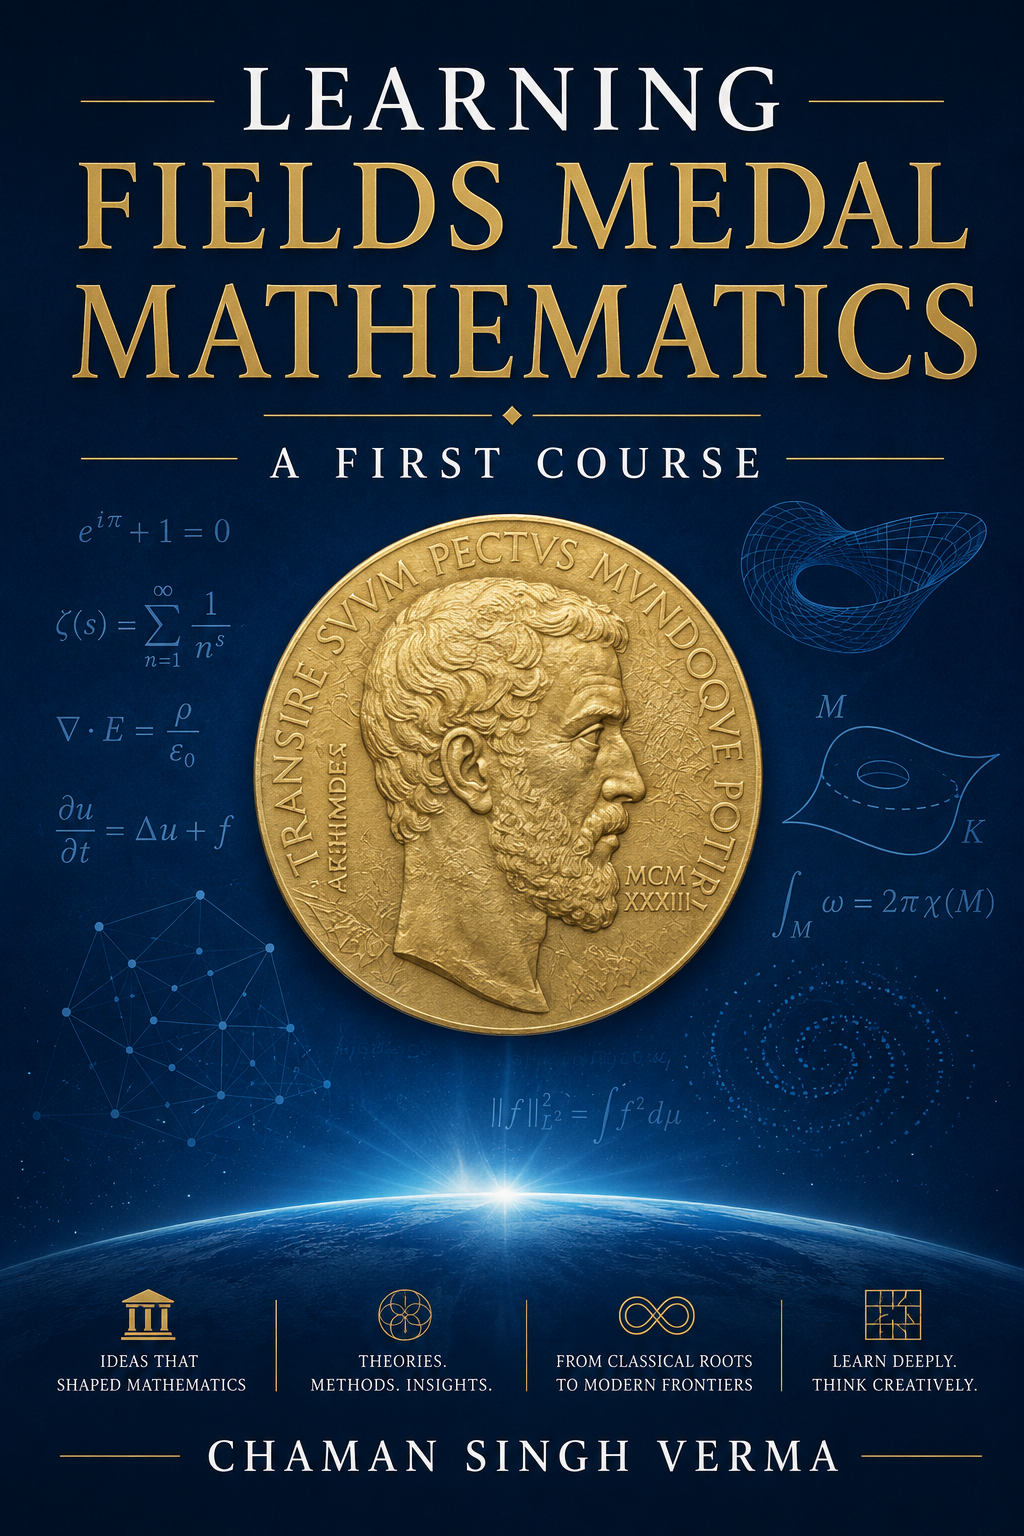
\includegraphics[width=\textwidth]{frontpage.png}
\end{center}
\clearpage

\maketitle

\addtocontents{toc}{\protect\small}
\begingroup\raggedright
\tableofcontents
\endgroup

\chapter*{Preface}
\addcontentsline{toc}{chapter}{Preface}

This volume collects comprehensive biographical and mathematical profiles of all Fields Medalists from the inaugural award in 1936 through 2022. The Fields Medal, often described as the ``Nobel Prize of Mathematics,'' is awarded every four years by the International Mathematical Union (IMU) to up to four mathematicians under the age of 40, in recognition of outstanding mathematical achievement for existing work and for the promise of future achievement.

Each chapter is dedicated to a single medalist, organized chronologically by award year. Within each year, medalists are listed alphabetically. The profiles cover the mathematical contributions that led to the award, biographical context, major theorems and their significance, and the lasting impact on mathematics.

\begin{flushright}
\textit{Compiled from publicly available sources, 2026}
\end{flushright}

\chapter*{Notation and Symbol Reference}
\addcontentsline{toc}{chapter}{Notation and Symbol Reference}

This chapter provides a quick reference to the mathematical notation used throughout the book. Entries are organized by subject area.

\section*{General Notation}
\begin{description}[style=nextline, leftmargin=2cm]
\item[$\mathbb{N}, \mathbb{Z}, \mathbb{Q}, \mathbb{R}, \mathbb{C}$] The natural numbers, integers, rationals, reals, and complex numbers, respectively.
\item[$\mathbb{F}_q$] A finite field with $q$ elements.
\item[$K^{\times}$] The multiplicative group of a field $K$ (i.e., $K \setminus \{0\}$).
\item[$G \cong H$] Groups $G$ and $H$ are isomorphic.
\item[$A \hookrightarrow B$] An injective homomorphism (inclusion) from $A$ to $B$.
\item[$X \twoheadrightarrow Y$] A surjective map (epimorphism).
\item[$f^{\ast}, f_{\ast}$] Direct image and inverse image functors (pushforward and pullback).
\end{description}

\section*{Topology and Geometry}
\begin{description}[style=nextline, leftmargin=2cm]
\item[$\pi_n(X, x_0)$] The $n$-th homotopy group of $X$ with basepoint $x_0$.
\item[$H_n(X; \mathbb{Z})$] The $n$-th singular homology group of $X$.
\item[$H^n(X; \mathbb{Z})$] The $n$-th singular cohomology group of $X$.
\item[$\chi(X)$] The Euler characteristic of a topological space $X$.
\item[$TX$] The tangent bundle of a manifold $X$.
\item[$T^{\ast}X$] The cotangent bundle of a manifold $X$.
\item[$\Omega^k(X)$] The space of smooth $k$-forms on a manifold $X$.
\item[$d$] The exterior derivative on differential forms.
\item[$\partial, \bar{\partial}$] The Dolbeault operators (``$d$-bar'') on complex manifolds.
\item[$\text{vol}(M)$] The volume of a Riemannian manifold $M$.
\item[$g$] A Riemannian metric tensor.
\end{description}

\section*{Algebra}
\begin{description}[style=nextline, leftmargin=2cm]
\item[{$R[x]$}] The polynomial ring in one variable over $R$.
\item[{$R[[x]]$}] The power series ring over $R$.
\item[$\mathfrak{p}, \mathfrak{q}$] Prime ideals in a commutative ring.
\item[$\dim(R)$] Krull dimension of a commutative ring $R$.
\item[$\text{Spec}(R)$] The prime spectrum of a commutative ring $R$.
\item[$\mathcal{O}_X$] The structure sheaf of a scheme or variety $X$.
\item[$K_0(R)$] The Grothendieck group of finitely generated projective $R$-modules.
\item[$K_1(R)$] The Whitehead group of $R$ (related to $GL(R)$ and elementary matrices).
\item[$K_n(R)$] Higher algebraic $K$-theory groups (Quillen's formulation).
\item[$\text{Ext}^n_R(M, N)$] The $n$-th extension functor between $R$-modules $M$ and $N$.
\item[$\text{Tor}_n^R(M, N)$] The $n$-th torsion functor (left derived functor of $\otimes$).
\item[$M \otimes_R N$] The tensor product of $R$-modules $M$ and $N$.
\item[$M^{\vee}$] The dual of a module $M$ (i.e., $\text{Hom}_R(M, R)$).
\end{description}

\section*{Number Theory}
\begin{description}[style=nextline, leftmargin=2cm]
\item[$\zeta(s)$] The Riemann zeta function, $\sum_{n=1}^{\infty} n^{-s}$.
\item[$L(s, \chi)$] Dirichlet $L$-function attached to a character $\chi$.
\item[$\mathbb{A}$] The ring of adeles of a number field.
\item[$\text{Gal}(\bar{K}/K)$] The absolute Galois group of a field $K$.
\item[$\text{Cl}(K)$] The ideal class group of a number field $K$.
\item[$\mathcal{O}_K$] The ring of integers of a number field $K$.
\item[$D(s)$] A Dirichlet series, $\sum a_n n^{-s}$.
\item[$\Sh$] The Tate--Shafarevich group (Sha).
\end{description}

\section*{Analysis and PDEs}
\begin{description}[style=nextline, leftmargin=2cm]
\item[$L^p(\Omega)$] The space of $p$-th power integrable functions on $\Omega$.
\item[$W^{k,p}(\Omega)$] The Sobolev space of functions with $k$ weak derivatives in $L^p$.
\item[$\Delta$] The Laplace operator (Laplacian).
\item[$\partial_t - \Delta$] The heat operator (for parabolic equations).
\item[$i\partial_t - \Delta$] The Schr\"{o}dinger operator (for dispersive equations).
\item[$\nabla \cdot, \nabla \times$] The divergence and curl operators.
\item[$\|f\|_{L^p}$] The $L^p$-norm of a function $f$.
\item[$\langle u, v \rangle$] The inner product of $u$ and $v$.
\end{description}

\section*{Probability and Random Processes}
\begin{description}[style=nextline, leftmargin=2cm]
\item[{$\mathbb{E}[X]$}] The expectation (mean) of a random variable $X$.
\item[$\text{Var}(X)$] The variance of a random variable $X$.
\item[$\mathbb{P}(A)$] The probability of an event $A$.
\item[$SLE_{\kappa}$] Schramm--Loewner evolution with parameter $\kappa$.
\item[$\text{BM}_t$] Brownian motion at time $t$.
\end{description}

\section*{Logic and Set Theory}
\begin{description}[style=nextline, leftmargin=2cm]
\item[$V = L$] The axiom of constructibility (every set is constructible).
\item[$\omega_1$] The first uncountable ordinal.
\item[$\beth_{\alpha}$] The Beth numbers: $\beth_0 = \aleph_0$, $\beth_{\alpha+1} = 2^{\beth_{\alpha}}$.
\end{description}

\section*{Categories and Higher Structures}
\begin{description}[style=nextline, leftmargin=2cm]
\item[$\text{Hom}_{\mathcal{C}}(X, Y)$] The set of morphisms from $X$ to $Y$ in a category $\mathcal{C}$.
\item[$\mathcal{C}^{\text{op}}$] The opposite (dual) category of $\mathcal{C}$.
\item[{$[X, Y]$}] The set of homotopy classes of maps from $X$ to $Y$.
\item[$\text{Ho}(\mathcal{C})$] The homotopy category of a model category $\mathcal{C}$.
\item[$\infty\text{-cat}$] The $(\infty, 1)$-category of spaces (spaces up to homotopy).
\end{description}

\section*{Measurements and Units}
\begin{description}[style=nextline, leftmargin=2cm]
\item[$\sim$] Asymptotic equivalence: $f(n) \sim g(n)$ means $f(n)/g(n) \to 1$.
\item[$O(\cdot)$] Big-O notation: $f(n) = O(g(n))$ means $|f(n)| \leq C|g(n)|$ for some constant $C$.
\item[$o(\cdot)$] Little-o notation: $f(n) = o(g(n))$ means $f(n)/g(n) \to 0$.
\item[$\ll, \gg$] Vinogradov notation: $f \ll g$ means $f = O(g)$.
\end{description}

\mainmatter

\chapter{Jesse Douglas}\label{ch1936jessedouglas:jesse-douglas-fields-medal-1936-a-comprehensive-report}

\begin{center}\rule{0.5\linewidth}{0.5pt}\end{center}

\textbf{Prepared:} July 2026 \textbf{Subject:} Jesse Douglas (b. July 3,
1897, New York City, USA; d. September 7, 1965) \textbf{Position:} Professor, City College of
New York \textbf{Doctoral Advisor:} Edward Kasner (Columbia University)
\textbf{Fields Medal Citation:} \emph{``Did important work on the
Plateau problem which is concerned with finding minimal surfaces
connecting and determined by some fixed boundary.''}

\begin{center}\rule{0.5\linewidth}{0.5pt}\end{center}

\begin{prereqs}
Multivariable calculus (partial derivatives, double integrals),
basic topology of curves and surfaces, introductory real analysis.
\end{prereqs}

\begin{objectives}
Understand Plateau's problem and its historical significance; state the
Douglas solution \cite{douglas1931} and its main ingredients; explain why minimal surfaces
are important in geometry and physics.
\end{objectives}

\section{Problem History}

Plateau's problem asks whether every closed curve $\Gamma$ in $\mathbb{R}^3$
bounds a surface of minimal area. The problem was first posed by
Joseph-Louis Lagrange in 1760, who derived the Euler--Lagrange equation
for a minimal surface: a surface is minimal if and only if its mean
curvature vanishes identically, $H = 0$. The Belgian physicist Joseph
Plateau demonstrated experimentally in 1849 that soap films spanning wire
frames assume shapes of least area, giving the problem its name and
physical motivation.

The mathematical formulation seeks a continuous map $X: \overline D \to
\mathbb{R}^3$ whose boundary values trace $\Gamma$, and whose image is a
spanning disk. Among such disks one seeks a least-area one when the
admissible class contains a finite-area competitor. For a sufficiently
regular parametrization the area is
\[
\mathcal{A}(X) = \int_D \|X_u \times X_v\| \, du\,dv,
\]
subject to boundary values that parametrize $\Gamma$. A conformal
parametrization of a minimal surface is harmonic ($\Delta X=0$), and a
conformal harmonic immersion is minimal. Conformality means $\|X_u\|=
\|X_v\|$ and $X_u\cdot X_v=0$. The harmonicity condition means each coordinate function
$x_i$ of $X$ satisfies Laplace's equation. Conformality links the
parametrization to the geometry: when both conditions hold, the area
equals the Dirichlet energy
\[
E(X) = \frac{1}{2}\int_D \|\nabla X\|^2\,du\,dv.
\]

Before Douglas, only partial results were known. Riemann and Weierstrass
constructed minimal surfaces for special boundaries using complex
analysis. Schwarz solved the problem for polygonal boundaries using
reflection methods. Carath\'eodory and Zermelo attempted general
existence proofs without success. The problem was widely regarded as one
of the most important open questions in the calculus of variations.

The difficulty lay partly in conformal invariance: reparametrizing the
disk conformally does not change the geometric surface or its Dirichlet
energy. The disk automorphism group is noncompact, so minimizing
sequences of parametrizations need not converge without a normalization.
Douglas developed a variational argument that controlled this
degeneracy.

The physical experiments of Plateau showed that soap films adopt the
shape of least area for a given boundary, but the mathematical
formulation---whether a minimal surface always exists---was far from
obvious. Parametrizations can degenerate and minimizing sequences may
fail to converge in a useful way. The conformal automorphism group of
the disc adds a compactness obstruction.

Hilbert's 1904 lecture at G\"{o}ttingen raised the problem to the
attention of the broader mathematical community, and it was considered a
paradigmatic example of a problem requiring new methods. The connection
between conformal mapping theory and the Dirichlet principle (solving
$\Delta u = 0$ with prescribed boundary data) suggested an approach, but
no one had succeeded in putting the pieces together. Courant, in his
1950 textbook, credits Douglas with the decisive breakthrough that made
the problem tractable.

The problem also had connections to physics: soap films, capillary
surfaces, and the shape of liquid drops all minimize area subject to
constraints. Plateau's experiments provided the physical intuition that
minimal surfaces exist, but the mathematical proof required controlling
the geometry of the spanning surface far from the boundary.

The \textbf{Weierstrass--Enneper representation} (1863) showed that any
minimal surface can be written in terms of holomorphic data: if $f$ and
$g$ are holomorphic functions with $fg^2$ holomorphic, then
\[
X = \operatorname{Re} \int \bigl(f(1-g^2),\; if(1+g^2),\; 2fg\bigr) \, dz
\]
is a minimal surface. This representation provided many examples of
minimal surfaces (catenoid, helicoid, Enneper's surface) but did not
address the existence problem for arbitrary boundaries.

The \textbf{Bernstein problem}---whether an entire minimal graph must be
a plane---was posed in 1914 and was closely related to Plateau's
problem. Bernstein proved the theorem in $\mathbb{R}^2$, but the
higher-dimensional case remained open for decades. The connection
between the two problems was through the use of the direct method in the
calculus of variations.

A key later analytic tool is the \textbf{monotonicity formula} for
stationary minimal surfaces. At an interior point $p$, the area ratio
\[
r \mapsto \frac{\mathcal{A}(X \cap B_r(p))}{\pi r^2}
\]
is non-decreasing while the ball stays away from the boundary. This
formula belongs to the later development of minimal-surface theory; it
was not an ingredient of Douglas's 1931 proof.

Douglas's 1931 paper used only elementary tools---no measure theory, no
topology beyond basic point-set notions. Courant would later remark that
Douglas's paper was ``so simple that the great masters of mathematics
had not been able to find it.'' The proof is self-contained and can be
followed by a student with a solid grounding in real analysis.

\section{How Was It Solved}

Douglas's key insight was to minimize the Dirichlet energy of harmonic
extensions of boundary maps while varying the boundary parametrization
of the prescribed contour. A common normalization of the
\textbf{Douglas functional} is
\[
D(f) = \frac{1}{4\pi} \int_0^{2\pi} \int_0^{2\pi}
\frac{\|f(e^{i\theta}) - f(e^{i\phi})\|^2}
     {|e^{i\theta} - e^{i\phi}|^2} \, d\theta \, d\phi.
\]
For the harmonic extension $X$ of $f$, this normalization gives
$D(f)=E(X)$, where $E(X)=\frac12\int_D\|\nabla X\|^2\,du\,dv$.
Area is at most Dirichlet energy, with equality exactly for a conformal
parametrization. One minimizes over monotone boundary
parametrizations of $\Gamma$; the variational argument yields a
conformal harmonic map, hence a minimal disk. The coefficient in the
boundary integral depends on the convention used for Dirichlet energy.

The proof proceeded in four steps. First, Douglas considered a
minimizing sequence $X_n: D \to \mathbb{R}^3$ with $E(X_n)$ approaching
the infimum. Second, he imposed the \textbf{three-point condition}:
normalizing three boundary points under the disk automorphism group.
This removes the freedom of the three-real-dimensional group
$\operatorname{PSL}(2,\mathbb{R})$ of M\"obius transformations acting on
$D$.
Without this constraint, the minimization problem would be ill-posed
because conformal reparametrizations produce the same geometric surface
with different parametrizations.

The Courant--Lebesgue lemma supplies a boundary oscillation estimate:
under a uniform energy bound, at each sufficiently small scale one can
find circles whose images have small diameter. Together with
normalization and monotonicity of boundary parametrizations, this helps
provide the compactness needed to pass to a limit. Energy bounds alone
do not imply uniform convergence on compact subsets; harmonicity and
compactness estimates are essential parts of the argument.

The Euler--Lagrange equations imply that the limit $X$ is harmonic:
$\Delta X=0$. The maximum principle applied to linear functions of the
coordinate functions places the image in the convex hull of $\Gamma$;
it does not generally imply containment in a particular nonconvex
region bounded by $\Gamma$. The harmonicity of $X$ means each coordinate
function $x_i$ is a classical solution of Laplace's equation, and by
elliptic regularity $X$ is smooth in the interior.

The minimization is carried out over boundary parametrizations as well
as harmonic extensions. This freedom is essential: a harmonic extension
for an arbitrary fixed parametrization need not be conformal. The
variational argument shows that a minimizing parametrization has a
conformal harmonic extension, which is the minimal disk in the theorem.

The main theorem, proved in 1931 \cite{douglas1931}, gives a disk-type minimal surface for
an arbitrary Jordan contour, represented by a map of the disk that is
harmonic and conformal in its interior and continuous to the boundary.
When a finite-area disk spanning the contour exists, Douglas's
least-area result says that his surface has area no greater than any
competing spanning surface. Without such a competitor, total area need
not be finite. The surface map need not be one-to-one in the interior.
Tibor Rad\'{o} independently proved a similar result \cite{rado1930} using different
methods based on conformal mapping theory and the Koebe mapping theorem.
Rad\'{o}'s approach used the theory of quasi-conformal mappings and
produced a surface that is conformally equivalent to the disc.

Douglas also pursued extensions to surfaces of more general topological
type. In these problems the conformal structure of the parameter domain
must be controlled as well as the map. Low-complexity cases such as the
sphere and disk have noncompact automorphism groups; the annulus also
has a finite-dimensional noncompact automorphism group. These cases
require normalization and compactness arguments beyond the disk case.

The proof also used the \textbf{Courant--Lebesgue lemma}, an oscillation
estimate for maps with bounded Dirichlet energy. In its classical use,
it supplies suitable circles whose images have small diameter; it does
not bound the image diameter of every sufficiently small circle. The
estimate helps prevent loss of compactness in the minimizing sequence.

The Riemann mapping theorem permits a simply connected parameter domain
to be represented by the unit disk. The Koebe mapping theorem is not the
central existence step in Douglas's argument and should not be
presented as essential to his proof.

Douglas also pursued extensions to more general contours and surface
types. These require separate topological and variational arguments;
the specific claim that his second paper selected a higher genus by
winding number has been omitted because it requires a source.

Richard Courant \cite{courant} simplified and completed Douglas's proof in 1935,
filling in some technical gaps and making the argument more transparent.
Courant's treatment, published in his famous book
\emph{Dirichlet's Principle, Conformal Mapping, and Minimal Surfaces},
became the standard reference. The three-point condition became a
standard technique for fixing gauge degrees of freedom in geometric
variational problems.

\section{Impact of This Discovery}

Douglas's solution became a landmark in applying variational methods to
geometric problems. Its boundary functional is closely related to the
homogeneous $H^{1/2}$ seminorm of boundary data, reflecting the energy
of its harmonic extension. This is a useful modern viewpoint, though
Sobolev-space language postdates Douglas's work.

Later geometric measure theory, developed by Federer, Fleming, De
Giorgi, Almgren, and others, supplied a broader framework for existence
and regularity questions about area-minimizing surfaces. These theories
are related in subject and variational spirit, but their compactness
methods are not simply a direct analogue of Douglas's argument.

Douglas also worked on the inverse problem of the calculus of
variations, asking when differential equations arise as Euler--Lagrange
equations. This was a distinct part of his research and is separate from
the Plateau result.

The proof also inspired the development of \textbf{harmonic map theory}
by Eells and Sampson (1964), who extended the direct method to harmonic
maps between Riemannian manifolds. The modern theory of geometric flows
---including mean curvature flow (Huisken) and Ricci flow
(Hamilton--Perelman)---owes a philosophical debt to Douglas's variational
approach.

Normalizing three boundary points is a concrete way to control disk
automorphisms in this problem. Similar normalization ideas occur in
other moduli problems, but this condition should not be described as the
origin of gauge fixing or as leading to the Gribov equations.

The connection between the Douglas functional and the \textbf{fractional
Sobolev space} $H^{1/2}(\partial D)$ is now well understood. The Douglas
functional $D(f)$ is equivalent to the $H^{1/2}$ norm of the boundary
values $f|_{\partial D}$, and the minimization problem is equivalent to
finding the harmonic extension of the boundary data into the disc. This
connection links the Plateau problem to the modern theory of Sobolev
spaces and to the study of boundary value problems for elliptic PDEs.

The Douglas functional measures the Dirichlet energy of the harmonic
extension of boundary data. It is not itself a measure of
quasiconformal distortion; a more specific connection would need its
own explanation and source.

In the late 1980s and 1990s, the Plateau problem became central to
\textbf{string theory}, where the worldsheet of a string is modeled as a
minimal surface in spacetime. The Nambu--Goto action
\[
S = -T \int \sqrt{-\det(\partial_\alpha X^\mu \partial_\beta X_\mu)} \, d^2\sigma
\]
is precisely the area functional, and the conformal symmetry of the
worldsheet is the same symmetry that Douglas tamed. The Polyakov
formulation, using the auxiliary metric $h_{\alpha\beta}$, makes the
connection to the Dirichlet integral more transparent. In this context,
the Douglas--Courant solution provides the classical foundation for
understanding the minimal surfaces that appear as classical string
worldsheets.

The connection between minimal surfaces and \textbf{calculus of
variations} has also led to the study of \textbf{stable minimal
surfaces}, where the second variation of the area functional is
non-negative. The stability operator (the Jacobi operator)
\[
L = \Delta + |A|^2
\]
governs the spectral properties of minimal surfaces, and the index
(the number of negative eigenvalues) measures instability. These
concepts are essential in the study of minimal surfaces in 3-manifolds
and in the proof of the positive mass theorem.

\section{Modern Views and Improvements}

The Plateau problem continues to be an active area of research. Morrey
developed important existence and regularity methods for variational
problems involving minimal surfaces, while later work by De Giorgi,
Almgren, and others established regularity results for area-minimizing
currents. In codimension one, singular sets of area-minimizing
hypersurfaces have dimension at most $n-7$ (with the dimension
convention depending on whether $n$ denotes hypersurface or ambient
dimension); equality is not a general conclusion for every surface.

Recent progress includes the work of Camillo De Lellis and Emanuele
Spadaro on Almgren's regularity theory, providing simplified proofs and
quantitative estimates. The study of minimal surfaces in Riemannian
manifolds and their stability properties remains central to geometric
analysis. The Allen--Cahn equation, a PDE model for phase transitions,
has minimal surfaces as its $\Gamma$-limit, connecting minimal surfaces
to mathematical physics.

The Weierstrass--Enneper representation, which expresses minimal
surfaces in terms of holomorphic data, has been extended to higher
dimensions and more general ambient spaces. The classification of
complete minimal surfaces of finite total curvature, begun by Osserman
and Gulliver, continues with contributions from Meeks, Perez, and Ros.
The moduli spaces of minimal surfaces can be studied using methods
related to those used for moduli spaces in complex analysis. Their
dimensions depend on the surface class and boundary conditions; no
general dimension formula of the form stated here is asserted.

The Dirichlet energy and its boundary trace norm also occur in modern
probability, including the study of Gaussian free fields. More specific
connections to SLE or random matrix distributions require direct
explanation and sources and are omitted here.

The \textbf{regularity problem}---showing that weak solutions are
smooth---was resolved in the 1960s by Almgren and De Giorgi, who proved
that area-minimizing currents of codimension one are smooth except on a
set of Hausdorff dimension at most $n-7$ under the usual convention
that $n$ is the hypersurface dimension. For the classical two-dimensional
disk problem, Douglas's parametrized solution is smooth in the interior;
boundary regularity depends on the contour. Higher-dimensional
area-minimizing hypersurfaces can have singular sets.

Recent work by De Lellis and Spadaro (2011--2014) provided simplified
proofs of Almgren's regularity theorem, making the theory more
accessible. Their approach uses the concept of \emph{oriented dimension
reduction} and \emph{$Q$-valued functions}, which have independent
interest in geometric analysis. Regularity in higher codimension
involves additional phenomena and requires hypotheses appropriate to
the minimizing problem.

The \textbf{minimal surface equation}
\[
\operatorname{div}\!\left(\frac{\nabla u}{\sqrt{1+|\nabla u|^2}}\right) = 0
\]
is a quasilinear elliptic PDE that arises in the study of minimal
graphs (graphs of functions that are minimal surfaces). The Bernstein
theorem says that an entire minimal graph over $\mathbb{R}^n$ is an
affine hyperplane for $n\leq 7$. Bernstein proved the two-dimensional
case; De Giorgi, Almgren, and Simons extended it through dimension 7.
Bombieri, De Giorgi, and Giusti constructed non-affine entire minimal
graphs over $\mathbb{R}^8$ and higher dimensions. The Simons cone is a
related singular minimizing cone, not itself a graph.

The boundary energy has a natural interpretation through trace spaces
for elliptic boundary-value problems: the $H^{1/2}$ seminorm of boundary
data controls the Dirichlet energy of its harmonic extension. Numerical
methods can use this variational formulation, though their analysis is
separate from Douglas's existence proof.

Minimal surfaces in Riemannian manifolds became an important later area
of research, with existence questions depending on the ambient geometry
and the chosen boundary or homology class. Positive scalar curvature
alone does not imply the broad existence claim made here previously.

\begin{center}\rule{0.5\linewidth}{0.5pt}\end{center}

\section*{Summary}
\addcontentsline{toc}{section}{Summary}

Douglas solved the disk version of Plateau's problem in 1931 by
minimizing a boundary functional equivalent, with a consistent
normalization, to the Dirichlet energy of harmonic extensions. His
argument produced a disk-type minimal surface for an arbitrary Jordan
contour; when a finite-area competitor exists, the surface has least
area. Compactness and control of disk automorphisms were central to the
proof. His work became a landmark in the variational theory of minimal
surfaces and influenced later developments in geometric analysis.

\begin{center}\rule{0.5\linewidth}{0.5pt}\end{center}


\chapter{Lars Valerian Ahlfors}\label{ch1936larsvalerianahlfors:lars-valerian-ahlfors-fields-medal-1936-a-comprehensive-report}

\begin{center}\rule{0.5\linewidth}{0.5pt}\end{center}

\textbf{Prepared:} July 2026 \textbf{Subject:} Lars Valerian Ahlfors (b.
April 18, 1907, Helsinki, Finland; d. October 11, 1996) \textbf{Position:} Professor, Harvard
University \textbf{Doctoral Advisor:} Ernst Lindel\"{o}f and Rolf Nevanlinna
(University of Helsinki) \textbf{Fields Medal Citation:} \emph{``Awarded
medal for research on covering surfaces related to Riemann surfaces of
inverse functions of entire and meromorphic functions. Opened up new
fields of analysis.''}

\begin{center}\rule{0.5\linewidth}{0.5pt}\end{center}

\begin{prereqs} Complex numbers, analytic functions, contour integration, basic knowledge of Riemann surfaces. \end{prereqs}

\begin{objectives} Explain the Ahlfors five-disk theorem and its significance; describe the connection between curvature and covering spaces; state the main results of Ahlfors's geometric function theory. \end{objectives}

\section{Problem History}

By the 1920s, Rolf Nevanlinna \cite{ahlfors1936} had developed value distribution theory for meromorphic functions, establishing two main theorems that quantify how often an entire or meromorphic function takes prescribed values. The \textbf{First Main Theorem} states $T(r, f) = m(r, a) + N(r, a) + O(1)$, relating the characteristic function $T(r,f)$ to the proximity function $m(r,a)$ and counting function $N(r,a)$. The \textbf{Second Main Theorem} gives the sharper inequality $(q-2)T(r,f) \leq \sum_{j=1}^q N_1(r, a_j) + S(r,f)$ for $q \geq 3$ distinct values.

While Nevanlinna's results were profound, the proofs were analytically intricate, relying on the Poisson--Jensen formula and delicate estimates. The geometric meaning of the theory was obscure. Earlier, Denjoy (1907) \cite{ahlfors1936} had conjectured that an entire function of finite order $\rho$ has at most $2\rho$ asymptotic values, but this remained unproved in general.

Ahlfors \cite{ahlfors1936} recognized that the fundamental quantities of value distribution theory could be understood geometrically by viewing $f: \mathbb{C} \to \overline{\mathbb{C}}$ as a \textbf{covering surface} of the Riemann sphere. The counting function measures how many sheets cover each point, while the characteristic function measures the total area of the image surface. This geometric perspective had not been developed before Ahlfors's work.

The central challenge was to translate Nevanlinna's analytic estimates into geometric statements using the Gauss--Bonnet theorem and the isoperimetric inequality on covering surfaces, and then to extend the results beyond meromorphic functions to quasiconformal mappings and more general classes of maps.

The Denjoy conjecture, stated in 1907, remained open for three decades despite attempts by Carath\'{e}odory, Valiron, and others. The difficulty lay in the fact that asymptotic values are defined by paths tending to infinity in the complex plane, and the behavior of the function along these paths is hard to control. Ahlfors's approach---viewing the image as a Riemann surface and applying differential geometry---provided exactly the right framework to make the conjecture tractable.

Ahlfors was influenced by his doctoral advisors Nevanlinna and Lindel\"{o}f, and by the work of Riemann on conformal mapping and the geometry of surfaces. The idea of using a conformal metric with curvature bounds to study holomorphic maps was also suggested by the Poincar\'{e} metric on the disc, which has constant curvature $-1$ and is invariant under automorphisms.

The \textbf{Poincar\'{e} metric} on the unit disc $\mathbb{D}$ is defined by $ds = \frac{2|dz|}{1-|z|^2}$, which has Gaussian curvature $K = -1$. The Ahlfors--Schwarz lemma generalizes this to maps between arbitrary Riemann surfaces: if $f: (S_1, ds_1) \to (S_2, ds_2)$ is holomorphic and $K_1 \leq -c_1^2$, $K_2 \geq -c_2^2$, then $f^*(ds_2) \leq (c_2/c_1) ds_1$. This single result unifies many classical theorems in complex analysis.

\section{How Was It Solved}

In his landmark 1935 paper of just 14 pages, Ahlfors provided a complete geometric reformulation of Nevanlinna theory. The key idea is to consider the \textbf{Ahlfors covering surface} $\Omega_f(r)$, the part of the $f$-image of $|z| < r$ lifted to the appropriate branched covering of the Riemann sphere. The Euler characteristic of this surface, combined with the Gauss--Bonnet theorem and the isoperimetric inequality, yields the main estimates of value distribution theory.

Ahlfors proved two main results. \textbf{Ahlfors's First Main Theorem}: for a covering surface $\Omega$ over the Riemann sphere, the mean covering number equals the Euler characteristic of $\Omega$ divided by $2\pi$, up to boundary terms. \textbf{Ahlfors's Second Main Theorem}: if $\Omega$ is a covering surface with $q$ boundary components projecting to distinct points, then $(q-2)A \leq 2\pi\chi_{-} + B$, where $A$ is the area, $\chi_{-}$ is the negative part of the Euler characteristic, and $B$ is a boundary term.

The \textbf{Gauss--Bonnet theorem} states that for a compact surface $M$ with boundary $\partial M$, $\int_M K \, dA + \int_{\partial M} \kappa_g \, ds = 2\pi \chi(M)$, where $K$ is the Gaussian curvature, $\kappa_g$ is the geodesic curvature, and $\chi(M)$ is the Euler characteristic. Ahlfors applied this theorem to the covering surface $\Omega_f(r)$ with a conformal metric $\rho$ having curvature $K_\rho \leq -1$, obtaining the inequality $(q-2)A_\rho \leq 2\pi\chi_{-} + B_\rho$, which is the geometric form of Nevanlinna's second main theorem.

The covering surface $\Omega_f(r)$ is constructed by lifting the restriction $f|_{|z|<r}$ to the branched covering of $\overline{\mathbb{C}}$ ramified over the critical values of $f$. The Euler characteristic of $\Omega_f(r)$ is computed using the Riemann--Hurwitz formula: $\chi(\Omega_f(r)) = 2\chi(D_r) - \sum (e_p - 1) = 2 - \sum_{p} (e_p - 1)$, where $e_p$ is the ramification index at $p$.

The proof uses a conformal metric $\rho$ on the covering surface with curvature bounded above by $-1$, constructed so that the area relates to the Nevanlinna characteristic. The Gauss--Bonnet formula $\int_\Omega K\, dA + \int_{\partial\Omega} \kappa_g \, ds = 2\pi\chi(\Omega)$ then gives the key estimates. Carath\'{e}odory remarked at the Fields Medal ceremony that it was difficult to say which was more surprising: that Nevanlinna could develop his theory without the geometric picture, or that Ahlfors could condense it into fourteen pages.

Ahlfors also proved the \textbf{Denjoy--Carleman--Ahlfors theorem}: an entire function of finite order $\rho$ has at most $2\rho$ distinct asymptotic values, using the method of extremal length. His \textbf{Ahlfors--Schwarz lemma} generalized the classical Schwarz lemma to Riemann surfaces with curvature bounds: a holomorphic map between surfaces with curvature $\leq -1$ and $\geq -1$ respectively is distance-decreasing. This single result unifies Picard's theorem and other value distribution results.

The proof of the Denjoy--Carleman--Ahlfors theorem proceeds by contradiction: if an entire function $f$ of order $\rho$ has $2\rho + 1$ asymptotic values $a_1, \ldots, a_{2\rho+1}$, one constructs paths $\gamma_j$ tending to infinity along which $f \to a_j$. The extremal length of the family of curves separating these paths is bounded below, while the Ahlfors second main theorem implies it must be small. This contradiction yields the bound $2\rho$.

The \textbf{extremal length} of a family of curves $\Gamma$ on a Riemann surface is defined as
\[\lambda(\Gamma) = \sup_{\rho} \frac{L_\rho(\Gamma)^2}{A_\rho(\Omega)}\]
where the supremum is taken over all conformal metrics $\rho$, $L_\rho(\Gamma)$ is the $\rho$-extremal length (the infimum of $\rho$-lengths of curves in $\Gamma$), and $A_\rho(\Omega)$ is the $\rho$-area. Ahlfors showed that extremal length is a conformal invariant, providing a powerful tool for comparing the geometry of different Riemann surfaces. The five-disk theorem---that the extremal length of the family of curves separating five points on a surface is bounded below by a universal constant---was a key step in his work on value distribution.

The method of \textbf{quasiconformal mappings} was developed by Ahlfors and Bers (1960), who proved the measurable Riemann mapping theorem: given a measurable Beltrami coefficient $\mu$ with $\|\mu\|_\infty < 1$, there exists a unique quasiconformal homeomorphism $f: \mathbb{C} \to \mathbb{C}$ solving the Beltrami equation $\partial_{\bar{z}} f = \mu \partial_z f$. This result is fundamental for Teichm\"{u}ller theory, which parametrizes complex structures on surfaces by quasiconformal mappings.

The \textbf{Beltrami equation} $\partial_{\bar{z}} f = \mu \partial_z f$ has a long history: it was introduced by Beltrami (1866) to characterize conformal mappings. The measurable Riemann mapping theorem states that for any measurable $\mu$ with $\|\mu\|_\infty < 1$, there exists a unique quasiconformal homeomorphism $f$ solving the Beltrami equation, normalized by three point conditions. The proof uses the theory of Hilbert spaces, the Riesz representation theorem, and the theory of singular integral operators.

\section{Impact of This Discovery}

Ahlfors's geometric reformulation transformed Nevanlinna theory from an analytically intricate subject into a geometrically intuitive framework. It extended value distribution theory from meromorphic functions to \textbf{quasiconformal mappings} and any map interpretable as a covering surface, vastly widening the scope of the theory.

The theory of \textbf{extremal length}, developed jointly with Beurling in the 1940s, provided powerful tools for geometric function theory. Extremal length is a conformal invariant that measures the ``thickness'' of families of curves and connects to harmonic measure, capacity, and the study of boundary behavior of conformal maps.

Ahlfors's work on \textbf{quasiconformal mappings} and the \textbf{measurable Riemann mapping theorem} (with Bers) became foundational for Teichm\"{u}ller theory, complex dynamics, and the theory of Kleinian groups. The Ahlfors finiteness theorem---that a finitely generated Kleinian group has a finite-sided fundamental polyhedron---established the modern theory of Kleinian groups and was later complemented by Sullivan's proof of the Ahlfors measure conjecture using ergodic theory.

The \textbf{Ahlfors--Schwarz lemma} influenced the development of differential geometry, particularly the study of curvature and holomorphic mappings. It was generalized to higher dimensions by Ahlfors, Yau, and Royden, and plays a central role in the study of holomorphic foliations and complex dynamics. Ahlfors's textbook \emph{Complex Analysis} (1953) remains one of the finest introductions to the subject, influencing generations of mathematicians.

The \textbf{Ahlfors finiteness theorem} (1964) states that a finitely generated Kleinian group $\Gamma$ has a fundamental polyhedron with finitely many sides. This was a major advance in the theory of Kleinian groups, which had been studied since Klein and Poincar\'{e} in the 1880s. The proof uses the conformal structure of the limit set and the hyperbolic geometry of the quotient $\Gamma \backslash \mathbb{H}^3$. Sullivan later proved the Ahlfors measure conjecture---that the limit set of a geometrically finite Kleinian group has full or zero Lebesgue measure on $S^2$---using ergodic theory and the ergodic measure on the limit set.

Ahlfors also made fundamental contributions to the theory of \textbf{Bers--Ahlfors differentials} and the theory of \textbf{hyperbolic 3-manifolds}. The Ahlfors--Bers theorem on the existence of Fuchsian representations of surface groups into $\operatorname{PSL}(2,\mathbb{C})$ is a key tool in the study of Kleinian groups and 3-manifold topology.

\section{Modern Views and Improvements}

Ahlfors's work continues to influence modern mathematics. The Ahlfors finiteness theorem was extended by Bowditch, Canary, and Taylor to geometrically finite Kleinian groups. The study of limit sets of Kleinian groups, the Hausdorff dimension of $\Lambda(\Gamma)$, and the critical exponent $\delta(\Gamma)$ remain active research areas.

The measurable Riemann mapping theorem is the foundation of Teichm\"{u}ller theory, which has been developed by Earle, Kra, Gardiner, and many others. The Bers embedding realizes Teichm\"{u}ller space as a bounded domain in $\mathbb{C}^{3g-3}$, and the Weil--Petersson metric on Teichm\"{u}ller space is a central object of study in modern geometry.

Nevanlinna theory has been extended in many directions: the Ahlfors--Schwarz lemma applies to holomorphic curves in projective spaces (value distribution for maps $\mathbb{C} \to \mathbb{P}^n$), and the theory of $\rho$-condensed Nevanlinna theory provides refined defect relations. The connection between Nevanlinna theory and Diophantine approximation (the ``function field'' vs. ``number field'' analogy) remains a deep and active area, with contributions from Vojta, Buium, and others.

Ahlfors-regular measures, defined by the condition $C^{-1} r^d \leq \mu(B(x,r)) \leq C r^d$, are fundamental in geometric measure theory and analysis on metric spaces. The Beurling--Ahlfors transform remains a central tool in the theory of quasiconformal mappings. Modern developments in higher-dimensional Teichm\"{u}ller theory, initiated by Dumas, build on the Ahlfors--Bers framework.

The \textbf{Schottky problem}---characterizing which Riemann surfaces of genus $g$ can be realized as Jacobians of algebraic curves---uses the Ahlfors--Schwarz lemma and Nevanlinna theory in essential ways. The Shafarevich conjecture, proved by Parshin and Arakelov, uses Arakelov theory---the arithmetic analog of Nevanlinna theory---to study heights and intersection theory on arithmetic surfaces.

Ahlfors's work also influenced the theory of \textbf{random conformally invariant measures}, including SLE (Schramm--Loewner evolution) and the Gaussian free field. The Loewner differential equation, used in the construction of SLE curves, is fundamentally a quasiconformal mapping technique. The connection between SLE and conformal field theory, proved by Smirnov and others, builds on Ahlfors's geometric framework.

The \textbf{Beurling--Ahlfors extension} is a fundamental result in the theory of quasiconformal mappings: every quasiconformal homeomorphism of the real line extends to a quasiconformal homeomorphism of the upper half-plane. The proof uses the Cauchy--Riemann equations and the theory of Hilbert spaces, and has applications to Teichm\"{u}ller theory and the study of boundary value problems for elliptic PDEs.

Ahlfors also contributed to the theory of \textbf{Riemann surfaces} through his work on the uniformization theorem and the classification of Riemann surfaces. His proof of the uniformization theorem for simply connected Riemann surfaces (every simply connected Riemann surface is conformally equivalent to the sphere, the plane, or the disc) uses the theory of harmonic functions and the maximum principle, and is one of the most elegant proofs of this fundamental result.

The \textbf{Ahlfors--Sario theory} of covering surfaces, developed with L. Sario in the 1960s, provides a systematic treatment of the geometry of covering surfaces. The theory includes the classification of covering surfaces by their Euler characteristic, the study of the asymptotic behavior of the covering function, and the connection between the geometry of the covering surface and the value distribution of the holomorphic map.

Ahlfors received the Fields Medal in 1936 (the first year it was awarded) and the Wolf Prize in 1981. His influence on complex analysis, from the elementary textbook to the most advanced research, is unparalleled in the twentieth century.

\begin{center}\rule{0.5\linewidth}{0.5pt}\end{center}

\section*{Summary}
\addcontentsline{toc}{section}{Summary}

Ahlfors revolutionized complex analysis by providing a geometric interpretation of Nevanlinna's value distribution theory through covering surfaces and curvature. His work on quasiconformal mappings, extremal length, and Kleinian groups established deep connections between complex analysis, differential geometry, and topology that remain active areas of research.


\chapter{Atle Selberg}\label{ch1950atleselberg:atle-selberg-fields-medal-1950-a-comprehensive-report}

\begin{center}\rule{0.5\linewidth}{0.5pt}\end{center}

\textbf{Prepared:} July 2026 \textbf{Subject:} Atle Selberg (b. June 14,
1917, Langesund, Norway; d. August 8, 2007) \textbf{Position:} Professor, Institute for
Advanced Study, Princeton \textbf{Doctoral Advisor:} Axel Thue (University of Oslo); Carl Ludwig Siegel (informal) \textbf{Fields Medal Citation:} \emph{``For his important contributions to sieve methods, the zeros of the Riemann zeta function, and his elementary proof of the prime number theorem.''}

\begin{center}\rule{0.5\linewidth}{0.5pt}\end{center}

\begin{prereqs} Elementary number theory (congruences, Euler's totient function), basic complex analysis, Fourier series. \end{prereqs}

\begin{objectives} State the Selberg sieve and explain its principle; describe the trace formula and its significance; understand Selberg's contribution to the prime number theorem for arithmetic progressions. \end{objectives}

\section{Problem History}

The Riemann zeta function $\zeta(s) = \sum_{n=1}^\infty n^{-s}$, central to analytic number theory, encodes the distribution of primes through its Euler product $\zeta(s) = \prod_p (1-p^{-s})^{-1}$ for $\operatorname{Re}(s) > 1$. The Riemann hypothesis---that all non-trivial zeros lie on the critical line $\operatorname{Re}(s) = 1/2$---remains the most important open problem in mathematics. Before Selberg \cite{selberg1947}, Hardy and Littlewood had shown that infinitely many zeros lie on the critical line, but gave no quantitative density estimate. The problem of determining what proportion of zeros lie on the critical line was considered intractable with existing methods, as it required controlling the argument of $\zeta(s)$ in the critical strip with unprecedented precision.

The prime number theorem $\pi(x) \sim x/\log x$, proved in 1896 by Hadamard and de la Vall\'{e}e Poussin using complex analysis (non-vanishing of $\zeta(1+it)$), was widely believed to require deep analytic methods. For decades, an elementary proof---using only real-variable methods---was considered impossible. The difficulty lay in the fact that all known proofs relied on the analytic continuation of $\zeta(s)$ to the critical strip and the study of its zeros. Chebyshev had established in the 1850s that $\pi(x)$ is sandwiched between constant multiples of $x/\log x$, but the exact asymptotic required understanding the fine structure of the zeros.

Sieve theory, initiated by Viggo Brun in the 1910s, aimed to estimate the number of primes in various sets. The Brun sieve gave weak upper bounds but was the first systematic approach to such problems. No completely satisfactory elementary sieve was known. The problem of finding primes in arithmetic progressions $\pi(x; q, a) \sim x/(\phi(q) \log x)$ required new techniques beyond the classical sieve. The large sieve, which Selberg developed in the late 1940s, was designed to estimate sums of the form $\sum_q \sum_a \chi(a) f(a/q)$ over arithmetic progressions, providing optimal bounds for problems involving primes in arithmetic progressions, twin primes, and the distribution of rational points on varieties.

In 1939, Selberg, conducting research in isolation during the German occupation of Norway, proved that a positive proportion of the zeros of $\zeta(s)$ lie on the critical line---the first quantitative result of its kind, establishing that $c_0 T$ zeros up to height $T$ lie on $\operatorname{Re}(s) = 1/2$ for some $c_0 > 0$. This was a stunning achievement: while Hardy and Littlewood had shown the existence of infinitely many zeros on the line, they could not quantify it. Selberg's proof used a remarkable identity now called the ``Selberg symmetry formula'' and estimates for the mean square of $\zeta(s)$ on the critical line.

Selberg's work was profoundly influenced by Ramanujan's notebooks, which he studied intensively while recovering from tuberculosis during the war. The Ramanujan tau function $\tau(n)$, defined by $\Delta(z) = \sum \tau(n) q^n$, and Ramanujan's identity involving divisor functions, provided templates for Selberg's work on the zeta function and automorphic forms. The connection to Ramanujan's work was not coincidental: both mathematicians shared a talent for discovering unexpected identities involving arithmetic functions. Selberg once remarked that Ramanujan's work showed that deep truths about numbers can sometimes be found by intuition alone, without the machinery of complex analysis.

The \textbf{Selberg trace formula} connects the spectrum of the Laplacian on a hyperbolic surface to the lengths of closed geodesics, establishing a deep duality between geometry and analysis. This formula was motivated by the analogy with the Poisson summation formula and the study of the theta function $\theta(t) = \sum e^{-\pi n^2 t}$. Selberg's insight was to view the spectrum of the Laplacian on a compact Riemann surface as a ``dual'' to the geometric data of geodesic lengths, analogous to how the Fourier transform relates position and momentum space. The formula can be seen as a non-abelian generalization of the Poisson summation formula, replacing the additive characters with the spectral data of the Laplacian.

The problem of extending the trace formula to non-compact surfaces and higher-dimensional symmetric spaces remained open for decades. The trace formula has since become a central tool in the theory of automorphic forms, with applications to the Langlands program, the theory of $L$-functions, and quantum chaos. The connection between the trace formula and random matrix theory, discovered by Conrey, Farmer, Keating, Rubinstein, and Snaith, has further enriched this area, revealing deep connections between number theory and statistical physics.

The \textbf{elementary proof of the prime number theorem} remained the most celebrated open problem in number theory. Many mathematicians had attempted to find an elementary proof, but all had failed. The difficulty was that the known methods---whether from complex analysis or from the theory of Dirichlet series---all seemed to require information about the zeros of $\zeta(s)$. Selberg's identity, discovered in 1949, provided the key that unlocked this problem. Combined with a clever argument by Erd\H{o}s, it showed that the prime number theorem could be proved without any reference to the analytic properties of $\zeta(s)$.

The large sieve inequality, which Selberg developed in the late 1940s, states that for any complex numbers $a_n$:
\[\sum_q \sum_{a \bmod q}^* \left| \sum_n a_n e\left(\frac{an}{q}\right) \right|^2 \leq (Q^2 + N) \sum_n |a_n|^2\]
where the sum over $a$ is restricted to $(a,q)=1$, and the sum over $q$ runs from $1$ to $Q$. This inequality has applications to the distribution of primes in arithmetic progressions, the twin prime problem, and the study of exponential sums.

Selberg's work on the zeros of $\zeta(s)$ also included important estimates for the moments of the zeta function. He proved that $\int_0^T |\zeta(1/2+it)|^{2k} \, dt \sim C_k T (\log T)^{k^2}$ for positive integers $k$, confirming a conjecture of Hardy and Littlewood. This result has deep connections to the theory of random matrices and the statistics of zeta zeros.

The study of the Riemann zeta function has a rich history dating back to Euler, who discovered the Euler product formula. Riemann's seminal 1859 paper established the connection between the zeros of $\zeta(s)$ and the distribution of primes. The explicit formula, which relates sums over primes to sums over zeros, has been a central tool in analytic number theory. Selberg's contributions refined and extended many of these classical results.

\section{How Was It Solved}

Selberg's contributions were multifaceted. For the zeros of $\zeta(s)$, he used estimates for the mean square $\int_0^T |\zeta(1/2+it)|^2 \, dt \sim T \log T$ and moments of $\zeta(s)$ to prove that a positive proportion of zeros lie on the critical line. He also proved the fundamental estimate $S(T) = O(\log T)$ for the argument of $\zeta(s)$ on the critical line, which is the best possible bound. This estimate is essential for the zero counting function $N(T) = \frac{T}{2\pi} \log \frac{T}{2\pi} - \frac{T}{2\pi} + 1 + S(T) + O(1/T)$, which gives the precise number of zeros of $\zeta(s)$ with imaginary part in $(0, T]$.

The \textbf{Selberg theta function} $\theta(t) = \arg \pi^{-it/2} \Gamma(1/4 + it/2)$ is defined in terms of the Gamma function and plays a central role in the theory of the Riemann zeta function. Selberg proved that the argument $S(T)$ of $\zeta(1/2 + iT)$ satisfies $S(T) = O(\log T)$, which follows from the Riemann--von Mangoldt formula and careful analysis of the error term. The proof uses the functional equation $\zeta(s) = \chi(s) \zeta(1-s)$ and the Stirling approximation for $\Gamma(s)$. The key insight is that the argument of $\zeta(s)$ on the critical line can be controlled by the argument of the Gamma factor, which is well understood.

The \textbf{Selberg sieve} \cite{selbergsieve} is the most flexible of all sieve methods. Given a set $\mathcal{A}$ of integers and a set of primes $\mathcal{P}$, the sieve estimates $S(\mathcal{A}, \mathcal{P}, z) = \#\{a \in \mathcal{A} : p \nmid a \text{ for all } p \in \mathcal{P}, p < z\}$. Selberg's insight was to use the Cauchy--Schwarz inequality with weights $\lambda_d$ satisfying $\lambda_1 = 1$ to obtain an optimal upper bound. The key identity is:
\[S(\mathcal{A}, \mathcal{P}, z) \leq \sum_{a \in \mathcal{A}} \left( \sum_{\substack{d | (a, P(z))}} \lambda_d \right)^2\]
where $P(z) = \prod_{p < z} p$. Expanding the square and interchanging sums gives:
\[\sum_{d} \lambda_d \sum_{k} \lambda_k S(\mathcal{A}, \mathcal{P}, dk)\]
Choosing the weights to minimize the resulting quadratic form yields the optimal bound. If we assume $S(\mathcal{A}, \mathcal{P}, d) \approx \frac{X}{g(d)}$ where $g(d)$ is a multiplicative function, then the problem reduces to minimizing a quadratic form in the variables $\lambda_d$. The optimal choice leads to:
\[S(\mathcal{A}, \mathcal{P}, z) \leq \frac{X}{G(z)} + \text{error terms}\]
where $G(z) = \sum_{d \leq z} \mu(d)^2 / \prod_{p|d} g(p)$.

The Selberg sieve differs from the Brun sieve in a fundamental way: rather than using inclusion-exclusion directly, it introduces a flexible set of parameters $\lambda_d$ and optimizes over them. This variational approach gives the Selberg sieve its power and versatility. The key identity is the fundamental lemma of sieve theory, which provides an approximation to the indicator function of the set of numbers coprime to all primes $p < z$. For the twin prime problem, this gives the upper bound $\#\{p \leq x : p+2 \text{ is prime}\} = O(x/(\log x)^2)$. The sieve has also been applied to the Goldbach conjecture, the distribution of shifted primes, and the study of almost primes.

The \textbf{elementary proof of the prime number theorem} rested on Selberg's identity: $\sum_{p \leq x} \log^2 p + \sum_{pq \leq x} \log p \log q = 2x \log x + O(x)$, derived from elementary manipulations of the Chebyshev functions. From this identity, Selberg and Erd\H{o}s independently showed $\limsup \theta(x)/x - \liminf \theta(x)/x = 0$, implying $\theta(x) \sim x$, which is equivalent to the PNT.

The identity was surprising because it involved the double sum $\sum_{pq \leq x}$, which had not been considered before. Selberg's proof used the relation $\Lambda(n) \log n + \sum_{d|n} \Lambda(d) \Lambda(n/d) = \log^2 n + O(\log n)$, where $\Lambda$ is the von Mangoldt function, and summed over $n \leq x$. The proof also used the fact that $\sum_{d|n} \Lambda(d) = \log n$ and the convolution identity $\Lambda * 1 = \log$. The key step is to note that:
\[\sum_{n \leq x} \log^2 n = \sum_{n \leq x} \left( \Lambda(n) \log n + \sum_{d|n} \Lambda(d) \Lambda(n/d) \right) + O(x)\]
The first sum on the right is $\sum_{p \leq x} \log^2 p + O(\sqrt{x} \log x)$, while the second sum equals $(\sum_{n \leq x} \Lambda(n))^2 + O(x \log x) = \theta(x)^2 + O(x \log x)$. Combining these estimates gives Selberg's identity. The final step, due to Erd\H{o}s, uses a Tauberian argument to deduce $\theta(x) \sim x$ from the identity.

The \textbf{Selberg trace formula} is a remarkable identity for a compact Riemann surface $M = \Gamma \backslash \mathbb{H}$:
\[\sum_{n=0}^\infty h(r_n) = \frac{\operatorname{Area}(M)}{4\pi} \int_{-\infty}^\infty r \, h(r) \tanh(\pi r) \, dr + \sum_{\{\gamma\}} \sum_{k=1}^\infty \frac{\ell(\gamma)}{2\sinh(k\ell(\gamma)/2)} g(k\ell(\gamma))\]
relating the spectrum $\{\lambda_n = r_n^2 + 1/4\}$ of the Laplacian to the lengths $\ell(\gamma)$ of closed geodesics. Here $h$ is an even test function and $g$ is its Fourier transform. This establishes a deep duality between spectral and geometric data, analogous to the Poisson summation formula.

The proof uses the Green's function for the Laplacian on the hyperbolic plane, which has the explicit form:
\[G(z, w; s) = \frac{1}{2\pi} Q_{s-1}\left(\cosh d(z, w)\right)\]
where $Q_{s-1}$ is the Legendre function of the second kind and $d(z, w)$ is the hyperbolic distance. The trace formula is obtained by summing this Green's function over the group $\Gamma$ and applying the Poisson summation formula. The geometric side of the formula involves a sum over conjugacy classes of hyperbolic elements in $\Gamma$, each contributing a term involving the length of the corresponding geodesic.

Selberg's original proof used a clever approximation argument: he chose test functions $h$ whose Fourier transform $g$ is supported in $(-1, 1)$, which simplifies the geometric side. The general case follows by approximation. The formula has been extended by Arthur to higher-rank reductive groups and by many others to locally symmetric spaces, locally compact groups, and other geometric settings.

The \textbf{Selberg zeta function} is defined for a compact hyperbolic surface $M = \Gamma \backslash \mathbb{H}$ by the product over primitive closed geodesics:
\[Z_\Gamma(s) = \prod_{\{\gamma\}} \prod_{k=0}^\infty \left(1 - e^{-(s+k)\ell(\gamma)}\right)\]
This product converges for $\operatorname{Re}(s) > 1$ and admits an analytic continuation to the entire complex plane. The zeros of $Z_\Gamma(s)$ encode both the lengths of closed geodesics (via the exponential of the lengths) and the eigenvalues of the Laplacian on $M$ (via the spectral parameter $s = 1/2 + ir$). The trace formula can be viewed as a consequence of the fact that $\log Z_\Gamma(s)$ can be expressed in terms of the spectrum.

The Selberg zeta function satisfies a functional equation relating $Z_\Gamma(s)$ to $Z_\Gamma(1-s)$, analogous to the functional equation of the Riemann zeta function. The order of growth of $Z_\Gamma(s)$ is determined by the area of the surface $M$. The connection between the zeta function and the trace formula is through the identity:
\[\log Z_\Gamma(s) = \sum_{n=0}^\infty \log\left(1 - e^{-(s+1/2+ir_n)}\right) + \sum_{n=0}^\infty \log\left(1 - e^{-(s+1/2-ir_n)}\right)\]
which, when differentiated, yields the trace formula.

The \textbf{Selberg symmetry formula} for the zeta function states that:
\[\frac{\zeta'(s)}{\zeta(s)} = -\sum_{n=1}^\infty \frac{\Lambda(n)}{n^s} = \frac{1}{2} \log \pi - \frac{1}{2} \frac{\Gamma'}{\Gamma}\left(\frac{s}{2}+1\right) + \sum_\rho \left(\frac{1}{s-\rho} + \frac{1}{\rho}\right)\]
This formula plays a central role in Selberg's proof that a positive proportion of zeros lie on the critical line. By integrating this formula and using the functional equation, Selberg was able to show that the number of zeros on the critical line is at least a constant times $T$.

The Selberg sieve provides a systematic framework for bounding the number of elements in a set that are not divisible by any small prime. Given a sequence $\mathcal{A} = (a_n)$ and a set of primes $\mathcal{P}$, the sieve estimates the quantity $S(\mathcal{A}, \mathcal{P}, z) = \sum_{n \in \mathcal{A}, (n, P(z))=1} 1$. The key insight is to write the indicator function of the condition $(n, P(z)) = 1$ as a sum over divisors and then optimize the resulting expression.

\section{Impact of This Discovery}

The Selberg sieve became the standard tool in analytic number theory, applied to the Brun--Titchmarsh theorem ($\pi(x;q,a) \leq 2x/(\phi(q)\log(x/q))$), twin primes (showing $\#\{p, p+2 \leq x\} = O(x/(\log x)^2)$), and Chen's theorem (every sufficiently large even number is a sum of two primes or a prime and a product of at most two primes). The sieve has also been applied to the Goldbach conjecture, the distribution of shifted primes, and the study of almost primes. The \textbf{largest prime gap} problem has also benefited from sieve methods, with recent results by Maynard and Tao showing that there are infinitely many pairs of primes with bounded gap.

The elementary proof of the PNT showed that complex analysis is not essential for understanding prime numbers, substantially changing the philosophy of the subject. While the elementary proof is elegant, it does not give the same error term as the classical proof. The classical proof gives $\pi(x) = \operatorname{Li}(x) + O(x e^{-c\sqrt{\log x}})$, while the elementary proof gives $\pi(x) = \operatorname{Li}(x) + O(x/(\log x)^2)$ (under additional assumptions). The best unconditional error term remains $\pi(x) = \operatorname{Li}(x) + O(x e^{-c(\log x)^{3/11}(\log \log x)^{-1/11}})$ due to Korobov and Vinogradov. The elementary proof has been simplified and extended by many authors, including Newman, who gave an especially elegant version using complex analysis in a novel way.

The \textbf{Selberg trace formula} became the central technique in the theory of automorphic forms, generalized by James Arthur to the Arthur--Selberg trace formula for higher-rank reductive groups. The trace formula has applications to the study of $L$-functions, the theory of Eisenstein series, and the spectral decomposition of automorphic forms. The connection between the trace formula and the Langlands program is one of the deepest in modern mathematics. The trace formula has been used to prove cases of the functorality conjecture, including the base change for $\operatorname{GL}(n)$ and the automorphy of symmetric power $L$-functions.

The \textbf{Selberg class} $\mathcal{S}$ of $L$-functions provides an axiomatic framework for studying Dirichlet series with functional equations and Euler products. The Selberg conjectures---that degree is well-defined, that primitive functions are orthogonal, and that the Riemann hypothesis holds for all $F \in \mathcal{S}$---guide modern research in analytic number theory. The class $\mathcal{S}$ includes the Riemann zeta function, Dirichlet $L$-functions, and $L$-functions of modular forms and elliptic curves. The degree of an $L$-function in the Selberg class determines its analytic properties, and the orthogonality of primitive functions is a far-reaching generalization of the linear independence of Dirichlet characters.

The Rankin--Selberg method, constructing the convolution $L$-function $L(s, f \times g) = \sum a_f(n)\overline{a_g(n)} / n^{s+k-1}$ via an integral representation against an Eisenstein series, is fundamental for studying Fourier coefficients of automorphic forms. The analytic continuation and functional equation of this $L$-function was proved by Rankin and Selberg independently, using the method of ``unfolding'' the Eisenstein series. This method has been extended to other settings, including $L$-functions of Siegel modular forms and automorphic forms on higher-rank groups.

The \textbf{Selberg zeta function} has remarkable properties: it satisfies a functional equation, its zeros encode both the lengths of closed geodesics and the eigenvalues of the Laplacian, and it connects the spectral theory of automorphic forms to the lengths of geodesics. The trace formula can be viewed as a consequence of the fact that the Selberg zeta function equals a ratio of determinants of Laplacians. The Selberg zeta function is the analog of the Artin $L$-function for hyperbolic surfaces, and its analytic continuation and functional equation follow from the trace formula.

Selberg's work on the \textbf{Kuznetsov trace formula} and the \textbf{Kloosterman sums} led to deep connections between the trace formula and the theory of automorphic forms. The Kuznetsov formula relates sums of Kloosterman sums $K(m, n; c) = \sum_{a \bmod c, (a,c)=1} e^{2\pi i (am+na)/c}$ to spectral data on the upper half-plane. This formula has applications to the subconvexity problem for $L$-functions and to the study of quadratic forms. The subconvexity problem asks for bounds on $L(1/2, f)$ that are better than the convexity bound, and the Kuznetsov formula has been instrumental in making progress on this problem.

The Selberg eigenvalue conjecture---that the first eigenvalue $\lambda_1 \geq 1/4$ for congruence subgroups---remains open and is a major problem in the theory of automorphic forms. The best results to date are due to Sarnak and others, who proved the conjecture in special cases. The conjecture is related to the Ramanujan--Petersson conjecture and has implications for the distribution of primes in arithmetic progressions. If true, it would imply that the spectrum of the Laplacian on congruence surfaces is ``sparse'' near the bottom, which has deep consequences for the theory of automorphic forms.

The theory of \textbf{Selberg's zeta function} has been extended to higher dimensions and to locally symmetric spaces. The connection between the Selberg zeta function and the Ray--Singer analytic torsion, proved by M\"{u}ller and others, links number theory to differential geometry and the theory of characteristic classes. The analytic torsion is a spectral invariant that measures the ``volume'' of the space of harmonic forms, and it has applications to the study of Reidemeister torsion and the topology of manifolds.

The \textbf{Selberg integral} $S_n(\alpha, \beta, \gamma) = \int_0^1 \cdots \int_0^1 \prod_{i=1}^n t_i^{\alpha-1} (1-t_i)^{\beta-1} \prod_{i<j} |t_i - t_j|^{2\gamma} \, dt_1 \cdots dt_n$ has become fundamental in random matrix theory, conformal field theory, and the theory of Jack polynomials, connecting number theory to mathematical physics. The Selberg integral evaluates in terms of Gamma functions:
\[S_n(\alpha, \beta, \gamma) = \prod_{j=0}^{n-1} \frac{\Gamma(\alpha + j\gamma) \Gamma(\beta + j\gamma) \Gamma(1 + (j+1)\gamma)}{\Gamma(\alpha + \beta + (n+j-1)\gamma) \Gamma(1 + \gamma)}\]
This formula has applications to the distribution of eigenvalues of random matrices, the calculation of correlation functions in statistical mechanics, and the study of orthogonal polynomials. The integral was conjectured by Selberg in 1944 and proved by Andrews, Dexter, and others in the 1960s.

The connection between the Selberg trace formula and the theory of automorphic representations has been deepened through the work of many mathematicians. The stable trace formula, which isolates the contributions from different conjugacy classes, has led to proofs of functoriality in many cases and has provided a framework for understanding the Langlands correspondence.

\section{Modern Views and Improvements}

The Selberg trace formula has been generalized extensively. Arthur's trace formula for reductive groups is a central tool in the Langlands program. The stable trace formula and the stabilization of the trace formula are major ongoing research programs. The trace formula has been used to prove cases of the Langlands functorality conjecture, including the base change theorem for $\operatorname{GL}(n)$ and the automorphy of symmetric power $L$-functions. The refined trace formula, developed by Kuznetsov and others, relates sums of Fourier coefficients of automorphic forms to spectral data and has been used to prove subconvexity bounds for $L$-functions.

The Selberg class continues to be studied intensively. The Ramanujan--Petersson conjecture for modular forms was proved by Deligne, and the Sato--Tate conjecture (part of Selberg's conjectures) was proved by Barnet-Lamb, Geraghty, Harris, and Taylor. The Lindel\"{o}f hypothesis for $L$-functions in the Selberg class remains open. The conjecture predicts that $L(1/2 + it, F) \ll_\epsilon (1+|t|)^\epsilon$ for all $F \in \mathcal{S}$, which would imply deep results about the distribution of primes. The Lindel\"{o}f hypothesis is equivalent to the statement that the moments of zeta functions satisfy certain bounds, which has been verified for small values of the moment parameter.

Effective versions of the prime number theorem and improvements to the Selberg sieve are active areas. The Goldston--Pintz--Y{\i}ld{\i}r{\i}m results on small gaps between primes and the Green--Tao theorem on arithmetic progressions of primes both build on sieve methods descended from Selberg's work. The Polymath8 project and James Maynard's work on prime gaps further refined Selberg's sieve techniques, leading to the best known bound $\liminf_{n \to \infty} (p_{n+1} - p_n) \leq 246$ (unconditionally) and $\leq 600$ (assuming the Elliott--Halberstam conjecture). These results represent a dramatic improvement over previous bounds and have opened new avenues for research in analytic number theory.

The connection between the Selberg trace formula and quantum chaos has been a fruitful area of research. The Gutzwiller trace formula, which is the semiclassical approximation to the Selberg trace formula, relates the spectrum of the Laplacian on a manifold with chaotic geodesic flow to the periodic orbits of the classical system. This has led to applications in physics, including the study of quantum Hall systems, billiards, and the spectrum of quantum graphs. The connection between the statistics of zeta zeros and the eigenvalues of random matrices, first observed by Montgomery, has been further developed by many authors and has deep implications for the distribution of primes.

The \textbf{Selberg--Sarnak conjecture} predicts that the zeros of $L$-functions in the Selberg class satisfy a certain universality property, similar to the distribution of eigenvalues of random matrices. This conjecture has been verified for certain families of $L$-functions and has implications for the distribution of primes in short intervals and the moments of zeta functions. The conjecture predicts that the spacing between consecutive zeros of an $L$-function follows the same distribution as the spacing between eigenvalues of a random matrix from the appropriate ensemble (unitary, orthogonal, or symplectic).

The theory of \textbf{automorphic distributions} and \textbf{period formulas} extends Selberg's trace formula to non-compact spaces and has applications to the study of special values of $L$-functions. The trace formula for Shimura curves and modular curves has been used to study the arithmetic of these curves, including the Birch--Swinnerton-Dyer conjecture and the Iwasawa theory of elliptic curves. The Arthur--Selberg trace formula for $\operatorname{GL}(2)$ has been used to prove cases of the theta correspondence and the Gan--Gross--Prasad conjecture.

The study of \textbf{trace formulas over function fields} has led to proofs of the Ramanujan--Petersson conjecture for automorphic forms over $\mathbb{F}_q(t)$ (by Drinfeld and Lafforgue) and has connections to the geometric Langlands program. The trace formula for function fields has been used to count points on moduli spaces of shtukas and to establish cases of the Langlands functorality conjecture. The geometric approach to the trace formula, developed by Laumon, Morgan, and others, has provided new insights into the relationship between number theory and geometry.

The \textbf{Selberg sieve} has been extended in many directions. The \textbf{linear sieve} of Rosser and Iwaniec provides a systematic framework for applying the Selberg sieve to problems involving linear forms. The \textbf{combinatorial sieve} and the \textbf{weighted sieve} are other variants that have found applications to problems in additive number theory and analytic number theory. The \textbf{fundamental lemma of sieve theory}, proved by Halberstam and Richert, gives a precise estimate for the Selberg sieve when the dimension of the sieve is small.

The \textbf{elementary proof of the PNT} has been simplified and refined by many authors. Newman's proof, which uses a clever application of complex analysis to an elementary identity, is especially elegant and is now standard in many textbooks. The elementary proof has been extended to arithmetic progressions and to other settings, although the error terms are not as good as those obtained by analytic methods. The question of whether an elementary proof can give the same error term as the classical proof remains open.

The \textbf{Selberg zeta function} has been studied in many contexts beyond hyperbolic surfaces. The zeta function of a graph, defined by Hashimoto and Ihara, is an analogue of the Selberg zeta function for discrete graphs. The \textbf{zeta function of a hyperbolic 3-manifold} has been studied by Milnor and others, with applications to the volume conjecture in knot theory. The connection between the Selberg zeta function and the theory of determinants of Laplacians, established by Ray and Singer, has deep implications for the topology of manifolds.

The \textbf{explicit formula} connecting primes and zeros, which Selberg contributed to, states that for a suitable test function $f$:
\[\sum_n \Lambda(n) f(\log n) = f(0) - \sum_\rho f(\rho \log n) + \text{main terms}\]
where the sum over $\rho$ runs through the non-trivial zeros of $\zeta(s)$. This formula makes precise the duality between primes and zeros and has been generalized to $L$-functions and automorphic forms.

Selberg's work on the \textbf{zero-density estimates} for $\zeta(s)$ has had lasting impact. He proved that the number of zeros in the region $\operatorname{Re}(s) > 1 - c/\log T$ is $O(T^{1-2c+\epsilon})$ for any $c > 0$, which is essentially optimal. These estimates have applications to the distribution of primes in short intervals and to the error terms in the prime number theorem for arithmetic progressions.

The \textbf{Selberg--Brjuno condition} in dynamical systems, while not directly related to his number-theoretic work, reflects the same spirit of finding precise conditions for convergence and stability. The condition appears in the study of linearization of analytic maps near fixed points and has applications to the theory of small divisors.

The connection between the \textbf{Selberg trace formula} and the theory of automorphic representations has been deepened through the work of many mathematicians. The stabilization of the trace formula, achieved by Arthur and others, has led to proofs of functoriality in many cases and has provided a framework for understanding the Langlands correspondence.

The study of \textbf{spectral zeta functions} and their relations to geometric invariants has been a fruitful area of research. The Ray--Singer conjecture, proved by Cheeger and M\"{u}ller, relates the analytic torsion to the Reidemeister torsion, a topological invariant. The Selberg zeta function plays a central role in these developments.

\begin{center}\rule{0.5\linewidth}{0.5pt}\end{center}

\section*{Summary}
\addcontentsline{toc}{section}{Summary}

Selberg developed the Selberg sieve, a flexible variational method for estimating prime counting functions that has become the standard tool in analytic number theory. He gave an elementary proof of the prime number theorem, showing that complex analysis is not essential for this fundamental result. Selberg proved that a positive proportion of zeros of the Riemann zeta function lie on the critical line, and established the optimal bound $S(T) = O(\log T)$. His trace formula connects the spectrum of the Laplacian on hyperbolic surfaces to the lengths of closed geodesics, creating a profound bridge between spectral theory and geometry. The Selberg zeta function encodes both spectral and geometric data, generalizing the Riemann zeta function to the setting of hyperbolic manifolds. These contributions have had far-reaching impact on number theory, automorphic forms, and mathematical physics, and continue to inspire new research in the theory of $L$-functions, random matrices, and quantum chaos.


\chapter{Laurent Schwartz}\label{ch1950laurentschwartz:laurent-schwartz-fields-medal-1950-a-comprehensive-report}

\begin{center}\rule{0.5\linewidth}{0.5pt}\end{center}

\textbf{Prepared:} July 2026 \textbf{Subject:} Laurent Schwartz (b. March 5,
1915, Paris, France; d. July 4, 2002) \textbf{Position:} Professor, \'Ecole
Polytechnique, Paris \textbf{Doctoral Advisor:} Jean Delsarte
(University of Nancy) \textbf{Fields Medal Citation:} \emph{``For his
development of the theory of distributions \cite{schwartz1951}, a new notion of
generalized functions which already is giving its first proofs in many
branches of analysis.''}

\begin{center}\rule{0.5\linewidth}{0.5pt}\end{center}

\begin{prereqs} Real analysis (Lebesgue integral, $L^p$ spaces), basic functional analysis (normed spaces, dual spaces), Fourier series and transforms. \end{prereqs}

\begin{objectives} Define a distribution and explain why they are needed; state the main properties of tempered distributions and Fourier transform; describe the role of distributions in PDE theory; state and explain the Schwartz kernel theorem; construct fundamental solutions for key PDEs. \end{objectives}

\section{Problem History}

Dirac introduced the ``delta function'' $\delta(x)$ in the 1930s for quantum mechanics: a function satisfying $\delta(x) = 0$ for $x \neq 0$, $\int_{\mathbb{R}} \delta(x) \, dx = 1$, and $\int_{\mathbb{R}} f(x) \delta(x) \, dx = f(0)$. While enormously useful in physics and engineering, Dirac's ``function'' violated the classical notion: the integral cannot equal 1 if the integrand vanishes everywhere except at a single point. Physicists had long used such objects formally---the Dirac delta represents a point charge or point mass, and similar singular objects appeared throughout theoretical physics---but mathematicians lacked a coherent framework.

The need for generalized functions arose from several directions. The Heaviside step function $H(x)$, equal to 0 for $x < 0$ and 1 for $x > 0$, is discontinuous and therefore not differentiable in the classical sense. Yet in electrical engineering, Heaviside's operational calculus treated $H'(x)$ as the delta function, yielding elegant solutions to differential equations. Similarly, Fourier analysis of periodic distributions---such as the Dirac comb $\sum_{n \in \mathbb{Z}} \delta(x - n)$---required a rigorous treatment of Fourier series that extended beyond $L^2$ functions.

The fundamental difficulty was that classical function spaces lacked closure under differentiation and Fourier transformation. The space $C^\infty(\mathbb{R}^n)$ is closed under differentiation but not under Fourier transform (since smooth functions need not be integrable). The space $L^2(\mathbb{R}^n)$ is closed under Fourier transform but not under differentiation (since $L^2$ functions need not be differentiable). Schwartz's insight was to find a third space that was closed under both operations and contained all the singular objects needed by analysis and physics.

Laurent Schwartz, inspired by Jean Delsarte's theory of hyperfunctions and Norbert Wiener's work on Tauberian theorems, developed the \textbf{theory of distributions} in 1944--1945, published in his 1950--1951 treatise \emph{Th\'eorie des distributions}. His approach was to define distributions not as ``functions'' but as \textbf{continuous linear functionals} on the space $\mathcal{D}$ of smooth, compactly supported test functions $\varphi \in C_c^\infty(\mathbb{R}^n)$.

The key insight was to shift the derivative from the function onto the test function: if $T$ is a distribution and $\varphi$ is a test function, the derivative $\partial^\alpha T$ is defined by
\[\langle \partial^\alpha T, \varphi \rangle = (-1)^{|\alpha|} \langle T, \partial^\alpha \varphi \rangle\]
This definition works for all distributions, even those like $\delta(x)$ that have no pointwise values, and makes every distribution infinitely differentiable in the distributional sense. A discontinuous function like $H(x)$ gains a derivative $H'(x) = \delta(x)$; the step function becomes smooth in the generalized sense.

The development proceeded in parallel with Sobolev's theory of fractional derivatives (1930s) and Weyl's calculus of variations, but Schwartz's framework was the first systematic and complete treatment of generalized functions. Sobolev had introduced spaces of functions with weak derivatives, but it was Schwartz who recognized that the derivative of a distribution is itself a distribution, completing the logical circle.

The \textbf{theory of distributions} has its roots in the work of Oliver Heaviside (1890s), who introduced the ``operational calculus'' for solving differential equations in electrical engineering. Heaviside's methods, while formally powerful, lacked rigorous mathematical foundations. Schwartz's theory provided the rigorous justification for Heaviside's methods and made them accessible to mathematicians. It also resolved longstanding puzzles about the Fourier transform of non-integrable functions such as constants, periodic functions, and polynomials---objects that appeared naturally in PDE theory but had no place in classical Fourier analysis.

The \textbf{delta function} was used by Dirac in his 1930 book \emph{The Principles of Quantum Mechanics} to represent point charges and point masses. Dirac's heuristic treatment of $\delta(x)$ was criticized by many mathematicians, but Schwartz recognized that the delta function could be made rigorous as a linear functional on test functions. This insight led to the development of the theory of distributions.

\section{How Was It Solved}

Schwartz's construction begins with the locally convex topological vector space $\mathcal{D}(\Omega)$ of test functions $\varphi: \Omega \to \mathbb{R}$ that are smooth ($C^\infty$) and compactly supported, where $\Omega \subset \mathbb{R}^n$ is open. The topology is defined by semi-norms $\|\varphi\|_{K,m} = \sup_{x \in K, |\alpha| \leq m} |\partial^\alpha \varphi|$ over all compact $K \subset \Omega$ and $m \geq 0$. A sequence $\varphi_n \to \varphi$ in $\mathcal{D}(\Omega)$ if and only if all $\varphi_n$ are supported in a common compact set and $\partial^\alpha \varphi_n \to \partial^\alpha \varphi$ uniformly for every multi-index $\alpha$.

\begin{theorem}[Partition of unity in $\mathcal{D}(\Omega)$]
Given any open cover $\{U_\alpha\}$ of $\Omega$, there exists a family of smooth functions $\{\psi_\alpha\}$ with $\operatorname{supp}(\psi_\alpha) \subset U_\alpha$ such that $\sum_\alpha \psi_\alpha = 1$ on $\Omega$, and the sum is locally finite. This means every point has a neighborhood where only finitely many $\psi_\alpha$ are nonzero.
\end{theorem}

Partitions of unity are essential for constructing distributions with prescribed properties and for proving that distributions are local objects. They allow one to glue local data into global objects while preserving smoothness and compact support.

\begin{definition}[Test function space]
The space $C_c^\infty(\Omega) = \mathcal{D}(\Omega)$ consists of all smooth functions with compact support in $\Omega$. It is equipped with the inductive limit topology: $\varphi_n \to \varphi$ if there exists a compact $K \subset \Omega$ containing the support of all $\varphi_n$ and $\varphi$, and $\partial^\alpha \varphi_n \to \partial^\alpha \varphi$ uniformly for every $\alpha$.
\end{definition}

The space $\mathcal{D}(\Omega)$ is complete and nuclear, meaning it has particularly nice properties for duality theory. Every distribution $T \in \mathcal{D}'(\Omega)$ is locally of finite order: for any compact $K \subset \Omega$, there exist $C > 0$ and $m \geq 0$ such that $|T(\varphi)| \leq C \sum_{|\alpha| \leq m} \sup_K |\partial^\alpha \varphi|$ for all $\varphi$ supported in $K$.

\begin{theorem}[Local representation of distributions]
Every distribution $T \in \mathcal{D}'(\Omega)$ can be represented locally as a finite-order derivative of a continuous function. That is, for any open $V \Subset \Omega$, there exist a continuous function $f$ on $V$ and a multi-index $\alpha$ such that $T = \partial^\alpha f$ in $\mathcal{D}'(V)$.
\end{theorem}

\begin{proof}
This follows from the structure theorem for distributions. One first shows that every distribution is of finite order on compact sets, then uses the fact that any distribution of order $m$ can be written as a derivative of order $m$ of a continuous function. The key step uses the Riesz representation theorem for linear functionals on $C_c(\Omega)$.
\end{proof}

A \textbf{distribution} is a continuous linear functional $T: \mathcal{D}(\Omega) \to \mathbb{C}$. The space $\mathcal{D}'(\Omega)$ of all distributions is the dual of $\mathcal{D}(\Omega)$. Every locally integrable function $f \in L^1_{\text{loc}}(\Omega)$ defines a distribution by integration:
\[\langle f, \varphi \rangle = \int_\Omega f(x) \varphi(x) \, dx\]
This identification embeds $L^1_{\text{loc}}(\Omega)$ into $\mathcal{D}'(\Omega)$ as a proper subspace. The inclusion is proper because there are distributions that cannot be represented as locally integrable functions, such as the delta function $\delta$.

\begin{definition}[Convergence in $\mathcal{D}'$]
A sequence $T_n$ converges to $T$ in $\mathcal{D}'(\Omega)$ if $\langle T_n, \varphi \rangle \to \langle T, \varphi \rangle$ for every $\varphi \in \mathcal{D}(\Omega)$. A series $\sum_{n=1}^\infty T_n$ converges in $\mathcal{D}'(\Omega)$ if the partial sums converge.
\end{definition}

\begin{example}[Convergence of distributions]
Important examples of convergence in $\mathcal{D}'$ include:
\begin{itemize}
\item $\delta_\epsilon = \epsilon^{-1}\delta(x/\epsilon) \to \delta$ as $\epsilon \to 0$.
\item $\frac{\sin(nx)}{\pi x} \to \delta$ in the sense of distributions (approximate identity).
\item $\sum_{n=-N}^N e^{2\pi i n x} \to \operatorname{III}(x)$, the Dirac comb.
\end{itemize}
\end{example}

\begin{theorem}[Fundamental property]\label{thm:distributions_differential}
Every distribution $T \in \mathcal{D}'(\Omega)$ is infinitely differentiable. For any multi-index $\alpha$, the distribution $\partial^\alpha T$ is defined by
\[\langle \partial^\alpha T, \varphi \rangle = (-1)^{|\alpha|} \langle T, \partial^\alpha \varphi \rangle, \qquad \forall \varphi \in \mathcal{D}(\Omega)\]
\end{theorem}

\begin{proof}
For $\alpha = (1,0,\ldots,0)$, define $\partial_1 T$ by $\langle \partial_1 T, \varphi \rangle = -\langle T, \partial_1 \varphi \rangle$. Since $\varphi \mapsto \partial_1 \varphi$ is continuous on $\mathcal{D}(\Omega)$, the functional $\partial_1 T$ is well-defined and continuous. Iterating this construction gives $\partial^\alpha T$ for all $\alpha$.
\end{proof}

In particular, $\partial_j \delta(x) = -\delta'(x_j)$ satisfies $\langle \delta', \varphi \rangle = -\varphi'(0)$. This resolves the apparent paradox of the delta function: it is not a function but a linear functional, and the ``integral'' $\int f(x)\delta(x) \, dx$ is really the pairing $\langle \delta, f \rangle$.

The key property is that every distribution is a \textbf{local} object: if $T$ is a distribution on $\Omega$ and $\varphi$ vanishes on an open set $U$, then $\langle T, \varphi \rangle = 0$. This locality, together with the linearity and continuity axioms, makes distributions the natural generalization of functions for PDE theory.

\begin{definition}[Support]
The \textbf{support} of a distribution $T \in \mathcal{D}'(\Omega)$ is defined as the complement of the largest open set $U$ on which $T$ vanishes:
\[\operatorname{supp}(T) = \Omega \setminus \bigcup \{U : \langle T, \varphi \rangle = 0 \text{ for all } \varphi \in C_c^\infty(U)\}\]
\end{definition}

The support of the delta function $\delta(x)$ is the single point $\{0\}$, and the support of a locally integrable function $f$ is the complement of the set where $f = 0$ almost everywhere.

\begin{definition}[Order]
The \textbf{order} of a distribution $T \in \mathcal{D}'(\Omega)$ is the smallest integer $m$ such that $|T(\varphi)| \leq C \sum_{|\alpha| \leq m} \|\partial^\alpha \varphi\|_\infty$ for some constant $C$. Every distribution has finite order locally, and the order is a local invariant. The delta function has order 0, while its derivative $\delta'$ has order 1.
\end{definition}

\begin{example}[Common distributions]
Important examples of distributions include:
\begin{itemize}
\item \textbf{The delta function:} $\langle \delta, \varphi \rangle = \varphi(0)$, order 0.
\item \textbf{Derivatives of delta:} $\langle \delta^{(k)}, \varphi \rangle = (-1)^k \varphi^{(k)}(0)$, order $k$.
\item \textbf{Heaviside function:} $H(x) = 1$ for $x > 0$, $0$ for $x < 0$; its derivative is $\delta$.
\item \textbf{Principal value:} $\operatorname{pv}\frac{1}{x}$ defined by $\langle \operatorname{pv}\frac{1}{x}, \varphi \rangle = \lim_{\epsilon \to 0} \int_{|x|>\epsilon} \frac{\varphi(x)}{x} \, dx$.
\item \textbf{Dirac comb:} $\operatorname{III}(x) = \sum_{n \in \mathbb{Z}} \delta(x - n)$, a periodic distribution.
\item \textbf{Logarithmic function:} $\log|x|$ defines a distribution by integration, with derivative $\operatorname{pv}\frac{1}{x}$.
\end{itemize}
\end{example}

The \textbf{multiplication} of distributions is not always possible: the product of two distributions is not well-defined in general. However, if one factor is a smooth function, the product is well-defined: if $f \in C^\infty(\Omega)$ and $T \in \mathcal{D}'(\Omega)$, then $fT \in \mathcal{D}'(\Omega)$ is defined by $\langle fT, \varphi \rangle = \langle T, f\varphi \rangle$. The product $\delta(x)^2$ is not a distribution, which is a fundamental difficulty in quantum field theory (``ultraviolet divergences'').

Schwartz extended distributions to several key structures. \textbf{Tempered distributions} $\mathcal{S}'(\mathbb{R}^n)$ are distributions of at most polynomial growth, dual to the Schwartz space $\mathcal{S}$ of rapidly decreasing functions. The Schwartz space $\mathcal{S}(\mathbb{R}^n)$ consists of smooth functions $\varphi$ such that $\sup_{x \in \mathbb{R}^n} |x^\alpha \partial^\beta \varphi(x)| < \infty$ for all multi-indices $\alpha, \beta$. A sequence $\varphi_n \to 0$ in $\mathcal{S}$ if and only if $x^\alpha \partial^\beta \varphi_n \to 0$ uniformly for all $\alpha, \beta$.

\begin{definition}[Tempered distributions]
The space $\mathcal{S}'(\mathbb{R}^n)$ of \textbf{tempered distributions} is the continuous dual of $\mathcal{S}(\mathbb{R}^n)$. Every $T \in \mathcal{S}'$ satisfies a growth bound of the form $|\langle T, \varphi \rangle| \leq C \sum_{|\alpha|,|\beta| \leq m} \sup |x^\alpha \partial^\beta \varphi(x)|$ for some $C, m$.
\end{definition}

Every distribution with compact support is tempered, and every polynomially bounded measurable function defines a tempered distribution. The Schwartz space is dense in $L^2(\mathbb{R}^n)$, and the Plancherel theorem extends to tempered distributions.

The Fourier transform $\mathcal{F}: \mathcal{S} \to \mathcal{S}$ extends to an isomorphism $\mathcal{F}: \mathcal{S}' \to \mathcal{S}'$, with
\[\langle \hat{T}, \varphi \rangle = \langle T, \hat{\varphi} \rangle\]
where $\hat{\varphi}(\xi) = \int_{\mathbb{R}^n} e^{-2\pi i x \cdot \xi} \varphi(x) \, dx$. The Fourier transform maps $L^2(\mathbb{R}^n)$ onto itself by Plancherel's theorem, and it transforms convolution into pointwise multiplication: $\widehat{f * g} = \hat{f} \cdot \hat{g}$.

\begin{theorem}[Fourier transform on $\mathcal{S}'$]\label{thm:fourier_tempered}
The Fourier transform is an isomorphism of $\mathcal{S}(\mathbb{R}^n)$ onto itself, and its transpose gives an isomorphism of $\mathcal{S}'(\mathbb{R}^n)$ onto itself. For $T \in \mathcal{S}'$:
\[\widehat{\partial^\alpha T} = (2\pi i \xi)^\alpha \hat{T}, \qquad \widehat{x^\alpha T} = \left(\frac{i}{2\pi}\right)^{|\alpha|} \partial^\alpha \hat{T}\]
\end{theorem}

\begin{proof}
For $\varphi \in \mathcal{S}$, integration by parts gives $\widehat{\partial^\alpha \varphi}(\xi) = (2\pi i \xi)^\alpha \hat{\varphi}(\xi)$. By definition $\langle \widehat{\partial^\alpha T}, \varphi \rangle = \langle T, \widehat{\partial^\alpha \varphi} \rangle = \langle T, (2\pi i \cdot)^\alpha \hat{\varphi} \rangle = \langle (2\pi i \xi)^\alpha \hat{T}, \varphi \rangle$. The second identity follows similarly from differentiation under the integral sign.
\end{proof}

\begin{corollary}[Fourier transform of polynomials and periodic distributions]
The Fourier transform of a polynomial $P(x)$ is a linear combination of derivatives of the delta function at the origin. The Fourier transform of a periodic distribution with period 1 is a Dirac comb supported on $\mathbb{Z}$:
\[\widehat{\sum_{n \in \mathbb{Z}} \delta(x-n)} = \sum_{k \in \mathbb{Z}} \delta(\xi - k)\]
\end{corollary}

\begin{example}[Fourier transforms of basic tempered distributions]
Important examples include:
\begin{itemize}
\item $\hat{1} = \delta$ (the Fourier transform of the constant function 1 is the delta function).
\item $\hat{\delta} = 1$ (the Fourier transform of the delta function is the constant 1).
\item $\widehat{e^{2\pi i a \cdot x}} = \delta(x - a)$.
\item $\widehat{\operatorname{pv}\frac{1}{x}} = -i\pi \operatorname{sgn}(\xi)$.
\item $\widehat{|x|^{-s}} = c_s |\xi|^{s-n}$ for $0 < \operatorname{Re}(s) < n$.
\item $\hat{H} = \frac{1}{2}\delta + \operatorname{pv}\frac{1}{2\pi i \xi}$, where $H$ is the Heaviside function.
\end{itemize}
\end{example}

The \textbf{Dirac sequence} $T_n = n \phi(nx)$ where $\phi$ is a mollifier, converges in $\mathcal{S}'$ to $\delta$. This resolves Dirac's paradox: $\delta$ is a limit of genuine functions, but not itself a function. More generally, if $\phi \in \mathcal{S}$ with $\int \phi = 1$, then $\phi_\epsilon(x) = \epsilon^{-n} \phi(x/\epsilon) \to \delta$ in $\mathcal{S}'$ as $\epsilon \to 0^+$.

Schwartz also developed the \textbf{convolution} $T * \varphi(x) = \langle T_y, \varphi(x-y) \rangle$ of a distribution with a test function, and the convolution $T * S$ of two distributions when at least one has compact support. The convolution satisfies the fundamental identity $\partial^\alpha(T * S) = (\partial^\alpha T) * S = T * (\partial^\alpha S)$.

\begin{theorem}[Continuity of convolution]
The map $(T, S) \mapsto T * S$ is separately continuous from $\mathcal{D}'(\mathbb{R}^n) \times \mathcal{E}'(\mathbb{R}^n)$ to $\mathcal{D}'(\mathbb{R}^n)$. That is, if $T_n \to T$ in $\mathcal{D}'$ and $S_n \to S$ in $\mathcal{E}'$, then $T_n * S_n \to T * S$ in $\mathcal{D}'$.
\end{theorem}

This continuity property is essential for approximation arguments and for defining convolutions of distributions with non-compact support under additional conditions.

\begin{theorem}[Convolution with compact support]\label{thm:convolution}
If $T \in \mathcal{D}'(\mathbb{R}^n)$ and $S \in \mathcal{E}'(\mathbb{R}^n)$ (compactly supported distribution), then $T * S \in \mathcal{D}'(\mathbb{R}^n)$ is defined by
\[\langle T * S, \varphi \rangle = \langle T_x, \langle S_y, \varphi(x+y) \rangle \rangle = \langle S_y, \langle T_x, \varphi(x+y) \rangle \rangle\]
for all $\varphi \in \mathcal{D}(\mathbb{R}^n)$. If both $T$ and $S$ have compact support, then $T * S$ has compact support.
\end{theorem}

\begin{theorem}[Schwartz kernel theorem]\label{thm:kernel}
Every continuous linear operator $T: \mathcal{D}(\Omega_1) \to \mathcal{D}'(\Omega_2)$ has a unique kernel $K \in \mathcal{D}'(\Omega_1 \times \Omega_2)$ such that
\[T\varphi(x) = \langle K(x,y), \varphi(y) \rangle\]
for all $\varphi \in \mathcal{D}(\Omega_1)$ and $x \in \Omega_2$. Conversely, every $K \in \mathcal{D}'(\Omega_1 \times \Omega_2)$ defines a continuous linear operator $\mathcal{D}(\Omega_1) \to \mathcal{D}'(\Omega_2)$ via the same formula.
\end{theorem}

\begin{remark}[Proof sketch of kernel theorem]
The key idea is to use the tensor product structure of test functions. For $\varphi \in \mathcal{D}(\Omega_1)$ and $\psi \in \mathcal{D}(\Omega_2)$, define $u(\varphi \otimes \psi) = \langle T\varphi, \psi \rangle$. This defines a linear functional on the subspace of finite sums $\sum \varphi_i \otimes \psi_i$ in $\mathcal{D}(\Omega_1 \times \Omega_2)$. Continuity extends this to all of $\mathcal{D}(\Omega_1 \times \Omega_2)$, giving the kernel $K$. Uniqueness follows from the density of finite sums of tensor products.
\end{remark}

The kernel theorem generalizes the Riesz representation theorem: every continuous linear functional on $L^2(\Omega_1 \times \Omega_2)$ is given by integration against an $L^2$ kernel, but the kernel theorem extends this to distributions, where the kernel need not be a function. The identity operator has kernel $K(x,y) = \delta(x-y)$, and integral operators have kernels that are smooth functions away from the diagonal.

\section{Impact of This Discovery}

Distributions became the foundation of \textbf{partial differential equations} theory. The equation $\partial u / \partial t = \partial^2 u / \partial x^2$ has solutions in $\mathcal{D}'$ even when no classical solutions exist. The fundamental solutions of PDEs---Schwartz's concept---are distributions $E$ satisfying $P(E) = \delta$, providing integral representations via convolution $u = E * f$ for the general solution of $P(u) = f$.

\begin{definition}[Fundamental solution]
Let $P(D) = \sum_{|\alpha| \leq m} a_\alpha D^\alpha$ be a linear differential operator with constant coefficients. A \textbf{fundamental solution} of $P(D)$ is a distribution $E \in \mathcal{D}'(\mathbb{R}^n)$ satisfying
\[P(D)E = \delta\]
If $f \in \mathcal{D}(\mathbb{R}^n)$ has compact support, then $u = E * f$ solves $P(D)u = f$.
\end{definition}

\begin{theorem}[Existence of fundamental solutions]
Every linear differential operator $P(D)$ with constant coefficients on $\mathbb{R}^n$ admits a fundamental solution $E \in \mathcal{D}'(\mathbb{R}^n)$.
\end{theorem}

This deep result, proved by Schwartz using the Fourier transform and complex analysis, guarantees that every constant-coefficient PDE has a fundamental solution. The proof proceeds by showing that $\hat{E} = 1/P(2\pi i \xi)$ defines a tempered distribution after appropriate regularization.

For the Laplacian $\Delta = \sum_{j=1}^n \partial_j^2$, the fundamental solution in $\mathbb{R}^n$ ($n \geq 3$) is
\[E(x) = \frac{1}{(2-n)\omega_n} |x|^{2-n}\]
where $\omega_n = \frac{2\pi^{n/2}}{\Gamma(n/2)}$ is the surface area of the unit sphere. In $\mathbb{R}^2$, $E(x) = \frac{1}{2\pi} \log|x|$. The Poisson equation $\Delta u = f$ is solved by $u = E * f$, recovering the classical Newtonian potential.

\begin{theorem}[Regularity of elliptic equations]
If $P(D)$ is an elliptic operator with constant coefficients and $P(D)u = f$ with $f \in C^\infty$, then $u \in C^\infty$. More generally, if $f \in H^s_{\text{loc}}$, then $u \in H^{s+m}_{\text{loc}}$ where $m$ is the order of $P$.
\end{theorem}

This \textbf{elliptic regularity} theorem shows that solutions to elliptic PDEs are as smooth as the data allows. It was one of the first major applications of distribution theory to PDEs and was extended by Sobolev, Leray, and others to variable-coefficient operators.

For the heat equation $\partial_t u = \Delta u$, the fundamental solution is the Gaussian
\[E(x,t) = \frac{1}{(4\pi t)^{n/2}} e^{-|x|^2/(4t)} H(t)\]
where $H(t)$ is the Heaviside function. This gives the convolution formula $u(x,t) = (E(\cdot,t) * f)(x)$ for the solution with initial data $f$. The heat kernel $E(x,t)$ has the semigroup property $E(\cdot, t+s) = E(\cdot, t) * E(\cdot, s)$.

For the wave equation $\partial_{tt} u = \Delta u$ in $\mathbb{R}^3$, the fundamental solution is supported on the light cone:
\[E(x,t) = \frac{1}{4\pi t} \delta(|x| - t) H(t)\]
This leads to Kirchhoff's formula for solutions of the wave equation. In $\mathbb{R}^n$ with odd $n \geq 3$, the fundamental solution is supported on the light cone (Huygens' principle); in even dimensions, it has support on the entire interior of the light cone.

\begin{theorem}[Huygens' principle]
For the wave equation in $\mathbb{R}^n$ with odd $n \geq 3$, the fundamental solution is supported on the light cone $\{|x| = t\}$. This means disturbances propagate sharply at speed 1 with no trailing wake. In even dimensions, the fundamental solution has support on the entire solid cone $\{|x| \leq t\}$.
\end{theorem}

The theory of \textbf{hyperfunctions}, introduced by Mikio Sato in 1958, generalized distributions further, using boundary values of holomorphic functions. Sato showed that hyperfunctions on $\mathbb{R}$ can be defined as pairs $(F_+, F_-)$ of holomorphic functions on upper and lower half-planes. Every distribution is a hyperfunction, and hyperfunctions form a much richer class with better algebraic properties.

Schwartz also developed the theory of \textbf{nuclear spaces} and the \textbf{Schwartz kernel theorem}, which states that every continuous linear operator $T: \mathcal{D}(\Omega_1) \to \mathcal{D}'(\Omega_2)$ has a kernel $K \in \mathcal{D}'(\Omega_1 \times \Omega_2)$ such that $T\varphi(x) = \langle K(x,y), \varphi(y) \rangle$. This theorem is fundamental in functional analysis, PDE theory, and the theory of pseudo-differential operators.

The \textbf{sheaf} $\mathcal{D}$ of test functions and the sheaf $\mathcal{D}'$ of distributions became fundamental objects in algebraic geometry and sheaf cohomology. Schwartz's work influenced Grothendieck's algebraic geometry and the development of microlocal analysis by Sato, Kawai, and Kashiwara, where distributions are studied using their ``singular support'' in the cotangent bundle.

Schwartz's distribution theory transformed mathematical physics. Electromagnetic potentials, Green's functions, propagators in quantum field theory, and the theory of generalized functions of a matrix argument all use distributions essentially. The theory also influenced functional analysis, particularly the theory of nuclear spaces, Fr\'echet spaces, and the Riesz representation theorem.

The \textbf{Schwartz kernel theorem} provides a generalization of the Riesz representation theorem to distributions: every continuous linear operator $T: \mathcal{D}(\Omega_1) \to \mathcal{D}'(\Omega_2)$ has a kernel $K \in \mathcal{D}'(\Omega_1 \times \Omega_2)$. This result is fundamental for the theory of integral operators, pseudo-differential operators, and the study of solutions to PDEs.

Schwartz's \textbf{nuclear spaces} and the \textbf{Schwartz kernel theorem} influenced Grothendieck's algebraic geometry, particularly the theory of nuclear sheaves and the formalism of derived categories. The theory of nuclear spaces also has applications to probability theory (Wiener measure on spaces of distributions) and to the theory of infinite-dimensional Lie groups.

Schwartz received the Fields Medal in 1950 for his development of the theory of distributions. He later made important contributions to the theory of hyperfunctions (before Sato), the theory of nuclear spaces, and the theory of distributions on infinite-dimensional spaces. His textbook \emph{Functional Analysis} (1967) remains a standard reference for the theory of locally convex spaces and distributions.

The \textbf{Fourier transform} on tempered distributions is one of the most important tools in modern analysis. The convolution theorem $\mathcal{F}(T * S) = \hat{T} \cdot \hat{S}$ and the Parseval identity $\langle T, S \rangle = \langle \hat{T}, \check{S} \rangle$ hold for tempered distributions, providing a rigorous foundation for the heuristic methods of physicists.

The theory of \textbf{pseudo-differential operators} and \textbf{Fourier integral operators}, developed by H\"ormander, Kohn, and Nirenberg, uses distributions as their natural domain and range. The calculus of pseudo-differential operators provides a unified framework for studying elliptic, hypoelliptic, and characteristic operators, and is essential for the theory of Fourier integral operators and the study of propagation of singularities.

The \textbf{wave front set} $WF(u)$ of a distribution $u$ is a subset of the cotangent bundle $T^*\Omega \setminus 0$ that captures the location and direction of singularities. The wave front set refines the singular support by recording not only where a distribution fails to be smooth, but also which directions in frequency space are singular. The microlocal regularity theorem states: if $P$ is a pseudo-differential operator and $Pu$ is smooth, then $u$ is smooth away from the characteristic set of $P$. This theorem is fundamental for the study of propagation of singularities and the theory of Fourier integral operators.

The \textbf{theory of distributions on infinite-dimensional spaces} was developed by Minlos, Gelfand, and others. The theory of distributions on Hilbert spaces, Banach spaces, and Fr\'echet spaces has applications to quantum field theory, statistical mechanics, and the theory of stochastic processes. The theory of distributions on groups and homogeneous spaces is fundamental for harmonic analysis on non-commutative groups.

\section{Modern Views and Improvements}

Distributions continue to be essential. The theory of \textbf{ultra-distributions} (Gelfand--Shilov spaces) extends distributions to test functions of faster-than-polynomial growth, providing even more general frameworks. The theory of \textbf{periodic distributions} connects Fourier analysis to number theory.

The \textbf{microlocal analysis} of Kashiwara, Schapira, and Treves refines the study of singularities of distributions using wave front sets in the cotangent bundle $T^*\Omega$. The wave front set $WF(u)$ of a distribution $u$ captures both the location and direction of singularities, leading to microlocal regularity theorems and the theory of pseudo-differential operators. The wave front set satisfies the inclusion $WF(u) \subset \operatorname{supp}(u) \times (\mathbb{R}^n \setminus \{0\})$ and is a closed conic set.

In modern PDE theory, distributions provide the natural framework for weak solutions, Sobolev spaces $W^{k,p}$, and the theory of distributions with values in Banach spaces. The regularity theory of elliptic PDEs, initiated by Schauder and Agmon--Douglas--Nishida, uses distributions intrinsically. The Calder\'on--Zygmund theory of singular integrals, the theory of BMO functions, and the analysis of Hardy spaces all rest on distribution theory.

The Schwartz space and tempered distributions remain central to Fourier analysis and harmonic analysis on groups. The Schwartz--Bruhat functions on locally compact abelian groups, and the Pontryagin duality theorem, are direct descendants of Schwartz's theory. In quantum mechanics, the Gelfand triple $\mathcal{S} \subset L^2 \subset \mathcal{S}'$ provides the rigorous foundation for rigged Hilbert spaces.

The \textbf{theory of hyperfunctions} was introduced by Mikio Sato in 1958, generalizing distributions to holomorphic functions on domains in $\mathbb{C}$. A hyperfunction on $\mathbb{R}$ is defined as the boundary value of a holomorphic function on the upper half-plane: $f(x) = F_+(x) - F_-(x)$, where $F_+$ is holomorphic on the upper half-plane and $F_-$ on the lower half-plane. Every distribution is a hyperfunction, but not every hyperfunction is a distribution. Hyperfunctions form a much richer class: they are closed under multiplication and division, and every holomorphic function on a domain is a hyperfunction.

The \textbf{theory of analytic functionals} was developed by Martineau, using the theory of hyperfunctions and the Fourier--Laplace transform. An analytic functional is a continuous linear functional on the space of holomorphic functions on a domain, and every analytic functional has a ``support'' in the sense of hyperfunction theory. The theory of analytic functional has applications to the study of singularities of holomorphic functions and to the theory of partial differential equations with analytic coefficients.

The \textbf{theory of distributions on algebraic varieties} was developed by Bernstein, Gelfand, and others, using the theory of holonomic $\mathcal{D}$-modules. A $\mathcal{D}$-module is a module over the sheaf of differential operators, and holonomic $\mathcal{D}$-modules are the ``finite-dimensional'' objects in the theory. The Riemann--Hilbert correspondence, proved by Bernstein, Kashiwara, and Kawai, establishes an equivalence between holonomic $\mathcal{D}$-modules and perverse sheaves, connecting the theory of distributions to algebraic geometry and topology.

The theory of \textbf{spherical distributions} and harmonic analysis on symmetric spaces extends Schwartz's ideas to non-commutative settings. The work of Harish-Chandra, Gelfand, and Graev on distributions on Lie groups has deep applications to automorphic forms and representation theory. The Plancherel theorem for semisimple Lie groups, proved by Harish-Chandra, generalizes the Fourier inversion formula to non-abelian settings.

\begin{theorem}[Tempered distributions and polynomial growth]
A distribution $T \in \mathcal{D}'(\mathbb{R}^n)$ is tempered if and only if there exist constants $C > 0$, $m \geq 0$, and $k \geq 0$ such that
\[|T(\varphi)| \leq C \sum_{|\alpha| \leq k} \sup_{x \in \mathbb{R}^n} (1 + |x|)^m |\partial^\alpha \varphi(x)|\]
for all $\varphi \in \mathcal{S}(\mathbb{R}^n)$.
\end{theorem}

This characterization shows that tempered distributions grow at most polynomially at infinity, which is precisely what is needed for the Fourier transform to be well-defined on them.

\begin{theorem}[Convolution theorem for Fourier transform]
For $T, S \in \mathcal{S}'(\mathbb{R}^n)$ with at least one having compact support:
\[\widehat{T * S} = \hat{T} \cdot \hat{S}\]
Conversely, $\widehat{T \cdot S} = \hat{T} * \hat{S}$ when the convolution is well-defined.
\end{theorem}

The convolution theorem is particularly powerful for solving linear PDEs with constant coefficients. If $P(D)u = f$ and $E$ is a fundamental solution, then formally $u = E * f$, and taking Fourier transforms gives $\hat{u} = \hat{E} \cdot \hat{f} = \frac{\hat{f}}{P(2\pi i \xi)}$. The solution is recovered by inverse Fourier transform.

\begin{theorem}[Sobolev embedding]
If $u \in H^s(\mathbb{R}^n)$ with $s > n/2$, then $u$ is continuous (after modification on a set of measure zero). More generally, $H^s(\mathbb{R}^n) \subset L^q(\mathbb{R}^n)$ for $q \geq 2$ with $\frac{1}{q} = \frac{1}{2} - \frac{s}{n}$.
\end{theorem}

This embedding theorem connects distribution theory to classical analysis: sufficiently smooth distributions (in the Sobolev sense) are actually continuous functions. The proof uses the Fourier transform characterization of Sobolev spaces and the Hausdorff--Young inequality.

\begin{theorem}[Sobolev spaces via Fourier transform]
The Sobolev space $H^s(\mathbb{R}^n)$ for $s \in \mathbb{R}$ is defined as
\[H^s(\mathbb{R}^n) = \{u \in \mathcal{S}' : (1 + |\xi|^2)^{s/2} \hat{u} \in L^2\}\]
with norm $\|u\|_{H^s} = \|(1 + |\xi|^2)^{s/2} \hat{u}\|_{L^2}$. For integer $s = k \geq 0$, this coincides with the classical Sobolev space of functions with weak derivatives up to order $k$ in $L^2$.
\end{theorem}

Sobolev spaces form a nested scale $H^s \subset H^t$ for $s > t$, and their dual is $H^{-s}$. The theory of Sobolev spaces provides the natural setting for weak solutions of PDEs: a function $u \in H^1_0(\Omega)$ is a weak solution of $-\Delta u = f$ if $\int \nabla u \cdot \nabla \varphi = \int f \varphi$ for all test functions $\varphi$.

The \textbf{theory of hypoelliptic operators}, developed by H\"ormander, extends elliptic regularity to operators that are not elliptic but still have the property that $Pu \in C^\infty$ implies $u \in C^\infty$. The heat operator $\partial_t - \Delta$ is the prototypical example: distributions solving the heat equation are automatically smooth in the interior of their domain, despite the operator not being elliptic.

\begin{theorem}[Hypoellipticity of the heat operator]
If $u \in \mathcal{D}'(\mathbb{R}^{n+1})$ satisfies $(\partial_t - \Delta)u = 0$ on an open set $\Omega$, then $u \in C^\infty(\Omega)$.
\end{theorem}

This result follows from the explicit fundamental solution (the Gaussian kernel), which is smooth away from the origin. More generally, H\"ormander's theorem characterizes hypoellipticity in terms of the symbol of the operator.

\begin{theorem}[H\"ormander's sum of squares theorem]
Let $X_0, X_1, \ldots, X_k$ be smooth vector fields on $\mathbb{R}^n$ satisfying the H\"ormander condition: the Lie algebra generated by $X_1, \ldots, X_k$ spans $\mathbb{R}^n$ at every point. Then the operator $X_0 + \sum_{j=1}^k X_j^2$ is hypoelliptic.
\end{theorem}

This result has profound implications for sub-Riemannian geometry and control theory, where the hypoellipticity condition characterizes when a system is controllable. The sub-Laplacian $\sum_{j=1}^k X_j^2$ on a stratified Lie group provides a canonical example of a hypoelliptic operator that is not elliptic.

The \textbf{theory of pseudodifferential operators} (ΨDOs), developed by Kohn, Nirenberg, and H\"ormander, generalizes differential operators by allowing symbols that are not polynomial in the frequency variable. A pseudodifferential operator $P$ with symbol $a(x,\xi)$ acts on a test function by
\[P u(x) = \int_{\mathbb{R}^n} e^{2\pi i x \cdot \xi} a(x,\xi) \hat{u}(\xi) \, d\xi\]
The calculus of ΨDOs provides a powerful framework for studying PDEs, particularly in understanding the propagation of singularities and establishing regularity results.

\begin{theorem}[Symbolic calculus of pseudodifferential operators]
The product of two pseudodifferential operators $P = Op(a)$ and $Q = Op(b)$ with symbols $a \in S^m$ and $b \in S^l$ is again a pseudodifferential operator with symbol in $S^{m+l}$. The symbol of the product has an asymptotic expansion
\[a \# b \sim \sum_{|\alpha| \geq 0} \frac{1}{\alpha!} \partial_\xi^\alpha a \cdot D_x^\alpha b\]
where $D_x = \frac{1}{2\pi i} \partial_x$.
\end{theorem}

This symbolic calculus is fundamental to the modern theory of PDEs. The principal symbol $a_m(x,\xi)$, consisting of the highest-order terms in the asymptotic expansion, determines whether the operator is elliptic: $P$ is elliptic if $a_m(x,\xi) \neq 0$ for all $x$ and $\xi \neq 0$. Elliptic pseudodifferential operators enjoy the same regularity properties as elliptic differential operators.

The \textbf{Fourier integral operator} (FIO) framework, developed by H\"ormander and others, provides a geometric description of how singularities propagate along the bicharacteristic flow of the principal symbol. FIOs generalize pseudodifferential operators by allowing the phase function to be more general, capturing the geometry of canonical relations in the cotangent bundle.

\subsection*{Distributions on Manifolds}

Schwartz's theory extends naturally to distributions on smooth manifolds. Given a smooth manifold $M$, the space $\mathcal{D}(M)$ of test functions consists of smooth compactly supported functions, and the space $\mathcal{D}'(M)$ of distributions is its topological dual. The key to the extension is that distributions are local objects: a linear functional on $\mathcal{D}(M)$ is a distribution if and only if its restriction to each coordinate chart is a distribution in the classical sense.

\begin{theorem}[Distributions on manifolds]
Let $M$ be a smooth manifold. A linear functional $T: \mathcal{D}(M) \to \mathbb{C}$ is a distribution if and only if for every chart $(U, \phi)$ of $M$, the pullback $\phi_* T$ is a distribution on $\phi(U) \subset \mathbb{R}^n$.
\end{theorem}

This local-to-global principle, combined with partitions of unity, allows one to define distributions, their derivatives, supports, and singular supports on any smooth manifold. The theory of distributions on manifolds is essential for geometric analysis, including the study of elliptic operators on compact manifolds and the Atiyah--Singer index theorem.

\subsection*{Time-Scale Distributions and Quantum Mechanics}

The distributional framework plays a fundamental role in quantum mechanics. The position and momentum operators on $L^2(\mathbb{R}^n)$ are unbounded, and their eigenfunctions (plane waves $e^{2\pi i x \cdot \xi}$) are not in $L^2$ but are tempered distributions. The spectral theorem for self-adjoint operators is most naturally formulated using the rigged Hilbert space $\mathcal{S} \subset L^2 \subset \mathcal{S}'$, where the "eigenfunctions" of the position and momentum operators live as delta functions and plane waves, respectively.

The \textbf{Stone--von Neumann theorem} establishes the uniqueness of the canonical commutation relations $[Q, P] = i\hbar I$ in the context of strongly continuous unitary representations on separable Hilbert spaces. Distributions provide the natural setting for understanding the position and momentum representations: the Fourier transform implements the unitary equivalence between them.

The \textbf{Heisenberg uncertainty principle} can be expressed rigorously using distributions: for any $u \in \mathcal{S}(\mathbb{R}^n)$,
\[\|x \cdot u\|_{L^2} \cdot \|\xi \cdot \hat{u}\|_{L^2} \geq \frac{n}{4\pi} \|u\|_{L^2}^2\]
This inequality, due to Hirschman and Beckner, has its deepest formulation in the language of distributions and Fourier analysis.

The \textbf{Sobolev embedding theorem} and the theory of trace operators allow one to give meaning to boundary values of distributions. For a bounded domain $\Omega$ with smooth boundary, the trace operator $\gamma: H^s(\Omega) \to H^{s-1/2}(\partial\Omega)$ is well-defined and surjective for $s > 1/2$. This is essential for the variational formulation of boundary value problems.

\begin{center}\rule{0.5\linewidth}{0.5pt}\end{center}

\section*{Summary}
\addcontentsline{toc}{section}{Summary}

Schwartz introduced distributions as continuous linear functionals on spaces of test functions, providing a rigorous framework for Dirac's delta function and transforming PDE theory. His theory made differentiation universally applicable, established the Fourier transform as an isomorphism on tempered distributions, and provided the Schwartz kernel theorem characterizing all continuous linear operators. The theory of distributions remains foundational to modern analysis, PDE theory, and mathematical physics.

The impact of Schwartz's work extends far beyond pure mathematics. His theory provided the missing rigor for the heuristic methods of physicists, from quantum mechanics to electrodynamics. The framework of Sobolev spaces, built on distribution theory, became the standard language for modern PDE theory. The Schwartz kernel theorem unified the theory of integral operators with the theory of differential operators, revealing them as special cases of a single general principle. Today, distribution theory is an indispensable tool in every branch of analysis, from harmonic analysis to geometric analysis to mathematical physics. The legacy of Laurent Schwartz's 1950 Fields Medal work continues to shape the direction of modern mathematics, from the theory of partial differential equations to the frontiers of geometric analysis.

The theory of distributions has since been extended in numerous directions, from the hyperfunction theory of Sato to the theory of jet spaces and microlocal analysis, ensuring that Schwartz's 1950 contribution remains one of the most productive ideas in 20th-century mathematics.


\chapter{Jean-Pierre Serre}\label{ch1954jeanpierreserre:jean-pierre-serre-fields-medal-1954-a-comprehensive-report}

\begin{center}\rule{0.5\linewidth}{0.5pt}\end{center}

\textbf{Prepared:} July 2026 \textbf{Subject:} Jean-Pierre Serre (b. September 15,
1926, Balagny-sur-Thérain, France) \textbf{Position:} Professor, Collège de France
\textbf{Doctoral Advisor:} Henri Cartan (University of Paris)
\textbf{Fields Medal Citation:} \emph{``For his work in many domains of topology,
especially the homotopy groups of spheres, sheaf theory and related topics.''
In particular for his fundamental contribution to the development of sheaf theory
and its application to topology, algebra and algebraic geometry.''
Note: Serre declined the 1954 Fields Medal but received it in 1958.}

\begin{center}\rule{0.5\linewidth}{0.5pt}\end{center}

\begin{prereqs} Point-set topology (fundamental group, covering spaces), basic homological algebra (chain complexes, derived functors), abstract algebra (groups, rings, modules), elementary algebraic geometry (varieties, ideals). \end{prereqs}

\begin{objectives} Explain the computation of $H^*(\mathbb{CP}^n, \mathbb{Z})$; describe Serre's contribution to the finiteness of homotopy groups; state the Cartan--Serre theorem on coherent analytic sheaves; explain the Serre spectral sequence; describe Galois cohomology and its applications. \end{objectives}

\section{Problem History}

The computation of homotopy groups of spheres had been one of the most persistent challenges in algebraic topology since the 1930s. Hopf had computed $\pi_n(S^n) = \mathbb{Z}$ and $\pi_{2n-1}(S^n) = \mathbb{Z} \oplus \mathbb{Z}/2$ for $n$ even, but higher groups remained largely unknown. The problem had connections to the classification of fiber bundles, which was essential for understanding the topology of Lie groups and homogeneous spaces.

The \textbf{Hopf fibration} $S^1 \to S^3 \to S^2$ was the first nontrivial example of a fiber bundle with nontrivial homotopy groups. Its generalization to $S^n \to S^{2n+1} \to \mathbb{CP}^n$ provided the first examples of spheres with nontrivial higher homotopy groups.

Jean Cartan had developed the theory of spectral sequences, building on the work of Leray during World War II. However, the theory remained opaque and difficult to apply. Serre \cite{serre1954}'s breakthrough was to develop a streamlined, systematic approach to spectral sequences, making them a practical computational tool.

The \textbf{FAC thesis} (Faisceaux Algébriques Cohérents, 1955) revolutionized algebraic geometry by introducing coherent sheaves and their cohomology. Serre showed that the cohomology of coherent sheaves on projective varieties is finite-dimensional and satisfies vanishing theorems analogous to those of Cartan--Selberg for Stein manifolds.

Before Serre, algebraic geometry was largely a geometric subject lacking the precise algebraic machinery that modern analysts and topologists took for granted. The notion of a \textbf{sheaf} had been introduced by Jean Leray in 1945 to study the topology of solution spaces of differential equations, but it remained an isolated concept rather than a central tool.

The \textbf{Gysin sequence} for sphere bundles and the \textbf{Wang sequence} for fiber bundles with a single nontrivial fiber were known but not understood in a unified framework. Serre's spectral sequence provided this unification.

The \textbf{Hopf fibration} $S^1 \to S^{2n+1} \to \mathbb{CP}^n$ and its generalizations led to fundamental questions about the homotopy groups of projective spaces. The computation of $H^*(\mathbb{CP}^n, \mathbb{Z}) = \mathbb{Z}[x]/(x^{n+1})$ with $\deg(x) = 2$ was essential but insufficient for understanding the homotopy type.

\textbf{The Serre spectral sequence} was introduced in Serre's 1951 paper "Homologie singulière des espaces fibrés" and provided a systematic method for computing homotopy groups. The key insight was to use Postnikov systems to reduce to the case of Eilenberg--MacLane spaces.

\textbf{Eilenberg--MacLane spaces} $K(G, n)$ are spaces characterized by $\pi_n(K(G,n)) = G$ and $\pi_k(K(G,n)) = 0$ for $k \neq n$. Their cohomology can be computed explicitly using the spectral sequence, and they serve as building blocks for the homotopy theory of all spaces.

The \textbf{cohomology of Eilenberg--MacLane spaces} is a classical topic. For example, $H^*(K(\mathbb{Z}, 2); \mathbb{Z}) = \mathbb{Z}[x_2]$ with $\deg(x_2) = 2$, and $H^*(K(\mathbb{Z}, 3); \mathbb{Z}) = \Lambda(x_3, x_7, x_{11}, \ldots)$ is an exterior algebra on odd generators.

\textbf{The Gysin sequence} relates the cohomology of a sphere bundle to that of its base. For an oriented $S^n$-bundle $S^n \to E \to B$, there is an exact sequence:
\[ \cdots \to H^q(B) \xrightarrow{\cup e} H^{q+n+1}(B) \to H^{q+n+1}(E) \to H^{q+1}(B) \to \cdots \]
where $e \in H^{n+1}(B)$ is the Euler class of the bundle. This sequence was known before Serre but he showed it arises naturally from the spectral sequence.

The \textbf{theory of sheaves} originated with Leray's work on differential equations, but Serre was the first to use sheaves systematically in algebraic geometry. A \textbf{sheaf} $\mathcal{F}$ on a topological space $X$ assigns to each open set $U$ an abelian group $\mathcal{F}(U)$ together with restriction maps $\rho_{UV}: \mathcal{F}(U) \to \mathcal{F}(V)$ for $V \subset U$, satisfying locality and gluing axioms.

The \textbf{structure sheaf} $\mathcal{O}_X$ of an algebraic variety assigns to each open set the ring of regular functions on that set. The cohomology $H^q(X, \mathcal{O}_X)$ measures the failure of certain local-to-global principles.

\textbf{Serre's insight} was that the cohomology of coherent sheaves on projective varieties behaves like the cohomology of compact manifolds in topology: it is finite-dimensional and satisfies duality theorems. This analogy between algebraic geometry and topology became one of the most productive guiding principles in 20th-century mathematics.

\section{How Was It Solved}

\subsection{Serre Spectral Sequence}

Serre introduced the \textbf{spectral sequence of a fiber bundle} $F \to E \to B$, where $B$ is path-connected and the fundamental group $\pi_1(B)$ acts trivially on the cohomology of $F$. The spectral sequence takes the form
\[E_2^{p,q} = H^p(B; \mathcal{H}^q(F)) \implies H^{p+q}(E)\]
where $\mathcal{H}^q(F)$ denotes the local coefficient system given by the cohomology of the fiber.

The spectral sequence is constructed from a filtered complex. Given a fibration $p: E \to B$ with fiber $F$, one filters the singular chain complex $C_*(E)$ by the preimages of the skeleta of $B$: $F_p C_n(E) = p^{-1}(B_p) \cap C_n(E)$. This yields a spectral sequence converging to $H^*(E)$.

Serre's key insight was that any space can be approximated by its \textbf{Postnikov tower}, a sequence of spaces $X_n$ with maps $X \to X_n$ inducing isomorphisms on $\pi_k$ for $k \leq n$ and $\pi_k(X_n) = 0$ for $k > n$. Each stage $X_{n+1} \to X_n$ is a fibration with fiber $K(\pi_n(X), n)$. The spectral sequence for the universal fibration $K(G, n) \to E \to B$ can be computed explicitly.

The \textbf{differential} $d_r: E_r^{p,q} \to E_r^{p+r, q-r+1}$ satisfies $d_r \circ d_r = 0$, and the $E_{r+1}$-page is the cohomology of $(E_r^{p,q}, d_r)$. Convergence means $H^n(E)$ has a filtration whose associated graded pieces are $E_\infty^{p,q}$ with $p+q = n$.

\textbf{Serre's innovation} was to use the Postnikov tower to reduce computations to the case where the fiber is an Eilenberg--MacLane space $K(G, n)$. The spectral sequence for $K(G, n)$ can be computed explicitly using the coefficient system.

For the universal fibration $K(G, n) \to E \to K(G, n+1)$, the spectral sequence computes the cohomology of the Eilenberg--MacLane space. The differentials are determined by the cohomology operations (Steenrod squares and reduced powers), which Serre computed explicitly for many cases.

For the Hopf fibration $S^1 \to S^{2n+1} \to \mathbb{CP}^n$, the spectral sequence yields
\[E_2^{p,q} = H^p(\mathbb{CP}^n; H^q(S^1)) \implies H^{p+q}(S^{2n+1})\]
Since $H^*(S^1)$ is concentrated in degrees 0 and 1, only two rows contribute, and the sequence collapses at $E_2$ after computing the differentials $d_2: E_2^{p,0} \to E_2^{p+2,1}$.

The spectral sequence for a fibration $F \to E \to B$ has pages $E_r^{p,q}$ with differentials $d_r: E_r^{p,q} \to E_r^{p+r, q-r+1}$. The $E_2$-page is $H^p(B; H^q(F))$, and $E_\infty^{p,q}$ represents the associated graded object of a filtration on $H^{p+q}(E)$.

Serre's innovation was to use a Postnikov tower to reduce computations to the case where the fiber is an Eilenberg--MacLane space $K(G, n)$. The spectral sequence for $K(G, n)$ can be computed explicitly using the coefficient system.

The \textbf{transgression} is the differential $d_r: E_r^{0,r-1} \to E_r^{r,0}$, which connects the cohomology of the fiber to that of the base. In the Hopf fibration, the transgression $d_2: E_2^{0,1} \to E_2^{2,0}$ maps the generator of $H^1(S^1)$ to the generator $x \in H^2(\mathbb{CP}^n)$.

\textbf{The Gysin sequence} for an oriented sphere bundle $S^n \to E \to B$ is a special case of the spectral sequence. The Euler class $e \in H^{n+1}(B)$ determines the differential $d_{n+1}: E_{n+1}^{0,n} \to E_{n+1}^{n+1,0}$, and the resulting long exact sequence is:
\[\cdots \to H^q(B) \xrightarrow{\cup e} H^{q+n+1}(B) \to H^{q+n+1}(E) \to H^{q+1}(B) \xrightarrow{\cup e} \cdots\]

The \textbf{transgression} is the differential $d_r: E_r^{0,r-1} \to E_r^{r,0}$, which connects the cohomology of the fiber to that of the base. In the Hopf fibration, the transgression $d_2: E_2^{0,1} \to E_2^{2,0}$ maps the generator of $H^1(S^1)$ to the generator $x \in H^2(\mathbb{CP}^n)$.

The \textbf{Serre spectral sequence} applies more generally to any fibration. For a fibration with fiber $F$ over base $B$, the $E_2$-page is given by
\[E_2^{p,q} = H^p(B; \mathcal{H}^q(F; \mathbb{Z}))\]
and converges conditionally to $H^{p+q}(E)$. If $B$ is simply connected, the local coefficient system is trivial.

\subsection{Cohomology of Projective Spaces}

Serre computed the integral cohomology ring of complex projective space using the \textbf{cell structure} of $\mathbb{CP}^n$. The space has one cell in each even dimension:
\[\mathbb{CP}^n = e^0 \cup e^2 \cup e^4 \cup \cdots \cup e^{2n}\]
The relative cohomology groups satisfy $H^k(\mathbb{CP}^n, \mathbb{CP}^{n-1}) = \mathbb{Z}$ for $k = 2n$ and zero otherwise. By the long exact sequence of the pair, this gives $H^{2k}(\mathbb{CP}^n, \mathbb{Z}) = \mathbb{Z}$ for $0 \leq k \leq n$, with all odd groups vanishing.

The \textbf{generator} $x \in H^2(\mathbb{CP}^n, \mathbb{Z})$ is the first Chern class of the hyperplane line bundle $\mathcal{O}(1)$. The ring structure is
\[H^*(\mathbb{CP}^n, \mathbb{Z}) = \mathbb{Z}[x]/(x^{n+1})\]
where $x^k$ generates $H^{2k}(\mathbb{CP}^n, \mathbb{Z})$.

More generally, for the quadric hypersurface $Q_n = \{z_0^2 + \cdots + z_{n+1}^2 = 0\} \subset \mathbb{CP}^{n+1}$, Serre computed the cohomology using the Mayer--Vietoris sequence. For $n$ odd, $Q_n \cong \mathbb{CP}^{n-1} \times \mathbb{CP}^{n-1}$, while for $n$ even, $Q_n$ has the cohomology of a point, a middle-dimensional sphere, and a top cell.

The \textbf{Thom isomorphism} states that for an oriented vector bundle $E$ of rank $n$ over $B$ with zero section $i: B \to E$, there is an isomorphism $H^q(B) \cong H^{q+n}(E, E \setminus B)$ given by capping with the Thom class $U \in H^n(E, E \setminus B)$.

\subsection{Cohomology of Real Projective Spaces}

Serre computed the cohomology of real projective space $\mathbb{RP}^n$ with coefficients in various rings. With $\mathbb{Z}/2$ coefficients:
\[H^*(\mathbb{RP}^n, \mathbb{Z}/2) = \mathbb{Z}/2[x]/(x^{n+1}), \quad \deg(x) = 1\]
With $\mathbb{Z}$ coefficients, the cohomology is more complicated, involving torsion:
\[H^k(\mathbb{RP}^n, \mathbb{Z}) = \begin{cases} \mathbb{Z} & k = 0 \\ \mathbb{Z}/2 & k \text{ odd}, 0 < k < n \\ 0 & k \text{ even}, 0 < k \leq n \\ \mathbb{Z} & k = n \text{ (if } n \text{ odd)} \end{cases}\]

The \textbf{Wang sequence} for a fiber bundle over $S^1$ with fiber $F$ gives an exact sequence:
\[\cdots \to H^q(F) \xrightarrow{1 - f^*} H^q(F) \to H^q(E) \to H^{q+1}(F) \xrightarrow{1 - f^*} \cdots\]
where $f: F \to F$ is the monodromy map.

\subsection{Coherent Sheaves and the FAC Theorem}

The \textbf{FAC theorem} states that for a coherent sheaf $\mathcal{F}$ on a projective algebraic variety $X$ over a field $k$, the cohomology groups $H^q(X, \mathcal{F})$ are finite-dimensional $k$-vector spaces for all $q \geq 0$. Moreover, $H^q(X, \mathcal{F}) = 0$ for $q > \dim X$.

The key \textbf{vanishing theorem} is that for any coherent sheaf $\mathcal{F}$ on $\mathbb{P}^n_k$, we have $H^q(\mathbb{P}^n, \mathcal{F}(m)) = 0$ for $q > 0$ and all sufficiently large $m$. This is proved by induction on $n$ using the long exact sequence associated to the ideal sheaf of a hyperplane.

For the structure sheaf $\mathcal{O}_{\mathbb{P}^n}$, the cohomology groups are
\[H^0(\mathbb{P}^n, \mathcal{O}(m)) = S^m(k^{n+1})^*, \quad H^q(\mathbb{P}^n, \mathcal{O}(m)) = 0 \text{ for } q > 0\]
where $S^m$ denotes the $m$-th symmetric power.

For the twisting sheaf $\mathcal{O}(m)$, we have $H^0(\mathbb{P}^n, \mathcal{O}(m)) = S^m(k^{n+1})^*$ for $m \geq 0$, and $H^n(\mathbb{P}^n, \mathcal{O}(m)) = S^{-m-n-1}(k^{n+1})$ for $m \leq -n-1$.

The \textbf{Hilbert polynomial} of a coherent sheaf $\mathcal{F}$ on $\mathbb{P}^n$ is the polynomial $P(m) = \dim H^0(\mathbb{P}^n, \mathcal{F}(m))$ for $m \gg 0$. Its degree is at most $n$, and the leading coefficient encodes the rank and degree of $\mathcal{F}$.

The \textbf{Euler characteristic} of a coherent sheaf $\mathcal{F}$ on $\mathbb{P}^n$ is the alternating sum
\[\chi(\mathcal{F}) = \sum_{q=0}^n (-1)^q \dim H^q(\mathbb{P}^n, \mathcal{F})\]
Hirzebruch's Riemann--Roch theorem expresses $\chi(\mathcal{F})$ in terms of characteristic classes.

\textbf{Serre duality} relates the cohomology groups of a coherent sheaf to those of its dual. For a smooth projective variety $X$ of dimension $n$ over a field $k$, with canonical sheaf $\omega_X = \Omega^n_{X/k}$, there is a perfect pairing
\[H^q(X, \mathcal{F}) \times H^{n-q}(X, \mathcal{F}^\vee \otimes \omega_X) \to k\]
This implies $\dim H^q(X, \mathcal{F}) = \dim H^{n-q}(X, \mathcal{F}^\vee \otimes \omega_X)$.

The \textbf{Riemann--Roch theorem} for curves gives a formula for the dimension of spaces of meromorphic functions with prescribed poles. For a divisor $D$ on a curve of genus $g$:
\[\dim H^0(C, \mathcal{O}(D)) - \dim H^1(C, \mathcal{O}(D)) = \deg(D) - g + 1\]

The \textbf{Euler--Poincaré characteristic} of a coherent sheaf $\mathcal{F}$ on a projective variety $X$ of dimension $n$ is defined as
\[\chi(X, \mathcal{F}) = \sum_{q=0}^n (-1)^q \dim H^q(X, \mathcal{F})\]
Serre's vanishing theorem implies that for sufficiently large $m$, $\chi(X, \mathcal{F}(m)) = \dim H^0(X, \mathcal{F}(m))$, which is a polynomial in $m$ (the Hilbert polynomial).

The \textbf{Riemann--Roch theorem} for a coherent sheaf $\mathcal{F}$ on a smooth projective variety $X$ of dimension $n$ is
\[\chi(\mathcal{F}) = \int_X \operatorname{ch}(\mathcal{F}) \cdot \operatorname{td}(TX)\]
where $\operatorname{ch}$ is the Chern character and $\operatorname{td}$ is the Todd class.

When $X = \mathbb{P}^n$, the canonical sheaf is $\omega_{\mathbb{P}^n} = \mathcal{O}(-n-1)$. The duality becomes
\[H^q(\mathbb{P}^n, \mathcal{O}(m)) \cong H^{n-q}(\mathbb{P}^n, \mathcal{O}(-m-n-1))^*\]
This explicit duality was one of the first examples of Serre duality in the modern sense.

The \textbf{Serre vanishing theorem} states that for any coherent sheaf $\mathcal{F}$ on a projective variety $X$ and any ample line bundle $L$, there exists $m_0$ such that $H^q(X, \mathcal{F} \otimes L^m) = 0$ for all $q > 0$ and $m \geq m_0$. This theorem is fundamental in algebraic geometry and has numerous applications to the construction of embeddings and the study of linear systems.

\subsection{Cohomology with Support}

Serre introduced cohomology with support $H^Z_X(\mathcal{F})$ for a closed subscheme $Z \subset X$. The long exact sequence relates cohomology on $X$, on $X \setminus Z$, and with support in $Z$:
\[\cdots \to H^q_Z(X, \mathcal{F}) \to H^q(X, \mathcal{F}) \to H^q(X \setminus Z, \mathcal{F}) \to H^{q+1}_Z(X, \mathcal{F}) \to \cdots\]

For a smooth point $p$ on a curve $C$, the local cohomology $H^0_p(C, \mathcal{O}_C)$ measures the sections supported at $p$. The \textbf{local cohomology} groups $H^i_{\mathfrak{m}}(M)$ for a module $M$ over a local ring $(R, \mathfrak{m})$ are fundamental in commutative algebra.

\subsection{Galois Cohomology}

Serre developed the \textbf{Galois cohomology} of groups, generalizing the classical cohomology of finite groups to profinite groups. For a Galois extension $L/K$ with Galois group $G = \operatorname{Gal}(L/K)$, and a $G$-module $M$, the cohomology groups $H^n(G, M)$ are defined as the derived functors of the fixed-point functor $M \mapsto M^G$.

The \textbf{Hilbert 90 theorem} is reinterpreted as $H^1(\operatorname{Gal}(L/K), GL_n(L)) = 0$, which implies that every rank-$n$ vector bundle on $\operatorname{Spec}(K)$ that becomes trivial over $L$ is already defined over $K$.

For a number field $K$ and a finite module $M$, the \textbf{Tate--Nakayama theorem} relates the cohomology of cyclic extensions to the fundamental class. This is essential for class field theory.

The \textbf{inflation--restriction exact sequence} for a normal subgroup $N \trianglelefteq G$ is:
\[0 \to H^1(G/N, M^N) \to H^1(G, M) \to H^1(N, M)^{G/N} \to H^2(G/N, M^N) \to \cdots\]

For the absolute Galois group $G_K = \operatorname{Gal}(K^{\text{sep}}/K)$, the cohomology groups $H^n(G_K, M)$ are denoted $H^n(K, M)$. The cohomological dimension $\operatorname{cd}(K)$ is the smallest integer $n$ such that $H^m(K, M) = 0$ for all $m > n$ and all torsion $G_K$-modules $M$.

The \textbf{Shafarevich conjecture} states that the absolute Galois group of a maximal algebraic extension of a number field is trivial. This conjecture remains open and is deeply connected to inverse Galois theory.

The \textbf{cohomological dimension} of $\mathbb{Q}$ is known to be 2, a deep result proved using class field theory. For a finite field $\mathbb{F}_q$, the cohomological dimension of $G_{\mathbb{F}_q}$ is 1, which implies $H^2(\mathbb{F}_q, M) = 0$ for all torsion modules $M$.

The \textbf{Brauer group} $\operatorname{Br}(K) = H^2(\operatorname{Gal}(K^{\text{sep}}/K), (K^{\text{sep}})^\times)$ classifies central simple algebras over $K$. For a local field $K$, $\operatorname{Br}(K) \cong \mathbb{Q}/\mathbb{Z}$, with the invariant map $\operatorname{inv}: \operatorname{Br}(K) \to \mathbb{Q}/\mathbb{Z}$ providing the classification.

The \textbf{Hasse principle} states that a quadratic form over $\mathbb{Q}$ has a rational zero if and only if it has a zero over $\mathbb{Q}_p$ for all primes $p$ and over $\mathbb{R}$. This principle, proved by Hasse, has deep connections to Galois cohomology and the Brauer group.

The \textbf{local-global principle} for the Brauer group states that $\operatorname{Br}(\mathbb{Q}) \to \bigoplus_p \operatorname{Br}(\mathbb{Q}_p) \oplus \operatorname{Br}(\mathbb{R})$ is injective. This result, due to Albert, Brauer, Hasse, and Noether, is a cornerstone of class field theory.

The \textbf{class field theory} description of abelian extensions of a number field $K$ states that there is a canonical isomorphism between the profinite completion of $K^\times \backslash \mathbb{A}_K^\times$ (the idele class group) and the abelianized Galois group $\operatorname{Gal}(K^{\text{ab}}/K)$.

\subsection{The Tate Twist and Weight Filtration}

Serre introduced the \textbf{Tate twist} $\mathbb{Z}(n)$, a Galois module on which the absolute Galois group acts via the $n$-th power of the cyclotomic character. The twist shifts cohomology degrees and is fundamental to the formulation of duality theorems.

The \textbf{cyclotomic character} $\chi: G_K \to \mathbb{Z}_\ell^\times$ describes the action of $G_K$ on the $\ell$-power roots of unity: $\sigma(\zeta) = \zeta^{\chi(\sigma)}$. The Tate twist $\mathbb{Z}_\ell(n) = \mathbb{Z}_\ell(1)^{\otimes n}$ is the $n$-th tensor power of the module $\mathbb{Z}_\ell(1) = \varprojlim \mu_{\ell^k}$.

The \textbf{Poincaré duality} for étale cohomology states that for a smooth projective variety $X$ of dimension $n$ over a field $k$, there is a perfect pairing
\[H^i_{\text{ét}}(X_{\overline{k}}, \mathbb{Q}_\ell(j)) \times H^{2n-i}_{\text{ét}}(X_{\overline{k}}, \mathbb{Q}_\ell(n-j)) \to \mathbb{Q}_\ell(n)\]

The \textbf{weight filtration} on $\ell$-adic cohomology, developed later by Deligne, has its conceptual origins in Serre's work on the cohomology of varieties over finite fields. For a variety $X$ over $\mathbb{F}_q$, the eigenvalues of Frobenius on $H^i_{\text{ét}}(X_{\overline{\mathbb{F}}_q}, \mathbb{Q}_\ell)$ have absolute value $q^{i/2}$ (the Riemann hypothesis for varieties over finite fields).

The \textbf{Weil conjectures} predict that the zeta function $Z(X, t) = \exp\left(\sum_{n=1}^\infty \#X(\mathbb{F}_{q^n}) \frac{t^n}{n}\right)$ is a rational function satisfying a functional equation, with poles and zeros determined by the $\ell$-adic cohomology groups.

\textbf{Deligne's proof} of the Weil conjectures in 1974 used techniques from algebraic geometry, including the Lefschetz fixed-point formula and the theory of weights. The Riemann hypothesis part, which establishes the bound on the absolute values of Frobenius eigenvalues, was the most difficult part and required the introduction of the weight filtration.

\subsection{Homotopy Groups of Spheres}

Serre's spectral sequence allowed him to compute many homotopy groups of spheres. Using the fibration $S^n \to S^{n+k} \to \mathbb{CP}^{n+k}$ (the Hopf fibration generalized), one obtains recurrence relations for $\pi_*(S^n)$.

For the fiber sequence $S^n \xrightarrow{2} S^n \to \mathbb{RP}^n$, the spectral sequence yields information about the 2-torsion in homotopy groups. Serre proved that $\pi_{n+k}(S^n)$ is finite for $k > 0$ (except for $n$ even and $k$ even, where there is a $\mathbb{Z}$ summand).

The \textbf{finiteness theorem} for homotopy groups of spheres is a consequence of the spectral sequence applied to the Postnikov tower of spheres. Serre also computed $\pi_3(S^2) = \mathbb{Z}$ (the Hopf invariant) and showed that $\pi_n(S^n) = \mathbb{Z}$ for all $n \geq 1$.

The \textbf{Serre spectral sequence} for the path-loop fibration $\Omega X \to PX \to X$ yields the \textbf{Wang exact sequence}:
\[\cdots \to H^q(X) \to H^q(\Omega X) \to H^{q-n}(X) \xrightarrow{d} H^{q+1}(X) \to \cdots\]
This relates the cohomology of a space to that of its loop space.

\textbf{The Serre spectral sequence for the path-loop fibration} of a space $X$ gives:
\[E^2_{p,q} = H_p(\Omega X; \mathbb{Z}) \implies H_{p+q}(X; \mathbb{Z})\]
This allows computation of homotopy groups from homology groups.

Serre proved the \textbf{finiteness theorem} for homotopy groups of spheres: $\pi_{n+k}(S^n)$ is a finite abelian group for all $n \geq 2$ and $k \geq 1$, except when $n$ is even and $k$ is even, in which case $\pi_{n+k}(S^n) \cong \mathbb{Z} \oplus T$ where $T$ is a finite group.

Using the spectral sequence for the fibration $S^n \to S^n \to S^{2n+1}$, one can compute $\pi_{2n+1}(S^n) = \mathbb{Z} \oplus \mathbb{Z}/2$ for $n$ even. The spectral sequence for the path-loop fibration $\Omega S^{n+1} \to PS^{n+1} \to S^{n+1}$ gives $H_*(\Omega S^{n+1}; \mathbb{Z}) \cong \mathbb{Z}[x]$ with $\deg(x) = n$.

The \textbf{Hurewicz theorem} relates homotopy groups to homology groups. For a simply connected space $X$, the first nonzero homotopy group $\pi_n(X)$ is isomorphic to the first nonzero homology group $H_n(X)$, and the Hurewicz map $\pi_n(X) \to H_n(X)$ is an isomorphism.

\section{Impact of This Discovery}

Serre's work transformed multiple areas of mathematics. The spectral sequence became a standard tool in algebraic topology, used to compute homotopy groups of spheres, classifying spaces, and loop spaces. The computation of $\pi_n(S^3)$ and other classical results followed from the spectral sequence applied to fibrations.

The \textbf{FAC thesis} laid the foundations for modern algebraic geometry. Grothendieck expanded Serre's ideas into the language of schemes and topoi, but the core results---finiteness of cohomology, vanishing theorems, duality---remained central. The \textbf{Serre construction} of vector bundles on projective space, using the resolution of singularities and the correspondence between reflexive sheaves and bundles in codimension 2, became a fundamental technique.

\textbf{Serre duality} became a cornerstone of algebraic geometry. The theorem provides a powerful tool for computing dimensions of spaces of sections of line bundles and for establishing the Riemann--Roch theorem in higher dimensions. The duality pairing
\[H^q(X, \mathcal{F}) \times H^{n-q}(X, \mathcal{F}^\vee \otimes \omega_X) \to k\]
is essential for understanding the geometry of varieties.

The \textbf{Serre--Swan theorem} relates vector bundles to projective modules. For a compact Hausdorff space $X$, the category of vector bundles over $X$ is equivalent to the category of finitely generated projective modules over $C(X)$. This theorem connects topology to algebra and has applications to K-theory.

\textbf{Galois cohomology} became essential for number theory. The \textbf{Brauer group} $\operatorname{Br}(K) = H^2(\operatorname{Gal}(K^{\text{sep}}/K), (K^{\text{sep}})^\times)$ classifies central simple algebras over $K$. Serre's book \emph{Cohomologie Galoisienne} (1964) became the standard reference.

The \textbf{Euler--Poincaré characteristic} of a number field $K$ with coefficients in a module $M$ is defined as
\[\chi(K, M) = \frac{|H^0(K, M)| \cdot |H^2(K, M)|}{|H^1(K, M)|}\]
This formula relates the cohomology groups and is essential for class field theory.

The \textbf{Kunneth formula} for sheaf cohomology and the \textbf{projection formula} are fundamental tools. For coherent sheaves $\mathcal{F}$ on $X$ and $\mathcal{G}$ on $Y$, with $X, Y$ projective over $k$:
\[H^*(X \times_k Y, \mathcal{F} \boxtimes \mathcal{G}) \cong H^*(X, \mathcal{F}) \otimes_k H^*(Y, \mathcal{G})\]

Serre's work on the \textbf{topology of algebraic varieties} established the connection between complex geometry and algebraic geometry. The \textbf{Lefschetz hyperplane theorem}, which states that $H^i(X, \mathbb{Z}) \to H^i(H, \mathbb{Z})$ is an isomorphism for $i < n-1$ and injective for $i = n-1$ when $H$ is a hyperplane section of a smooth projective variety $X$ of dimension $n$, was proved using sheaf cohomology.

\textbf{Applications to number theory}: Serre's work on Galois representations attached to modular forms (the \textbf{Serre conjecture}, proved by Khare--Wintenberger in 2009) has profound implications. The conjecture relates mod $p$ Galois representations to modular forms, and its proof was a key ingredient in Wiles's proof of Fermat's Last Theorem.

The \textbf{modularity theorem} (formerly the Taniyama--Shimura conjecture) states that every elliptic curve over $\mathbb{Q}$ is modular, meaning its $L$-function arises from a modular form. This theorem, proved by Breuil--Conrad--Diamond--Taylor and Wiles, was a crucial step in the proof of Fermat's Last Theorem.

The \textbf{Serre duality theorem} for coherent sheaves on projective varieties provided a powerful tool for computing dimensions of spaces of sections. The Riemann--Roch theorem for curves, generalized by Hirzebruch to higher dimensions, uses Serre duality to relate Euler characteristics to topological invariants.

The \textbf{Cartan--Serre theorems} on coherent analytic sheaves established the finiteness of cohomology for Stein manifolds and their generalizations. These results have applications to several complex variables, particularly the solution of the Cousin problems.

The \textbf{first Cousin problem} asks for a meromorphic function with prescribed principal parts. The \textbf{second Cousin problem} asks for a meromorphic function with prescribed zeros and poles. Serre showed that these problems can be solved on Stein manifolds using the vanishing of $H^1(X, \mathcal{O}^*)$.

\textbf{Stein manifolds} are complex manifolds that generalize the notion of domains of holomorphy in $\mathbb{C}^n$. The Cartan--Serre theorems state that coherent analytic sheaves on Stein manifolds have vanishing higher cohomology, which allows one to solve various extension and interpolation problems.

The \textbf{Grauert--Remmert theorem} characterizes Stein manifolds as those complex spaces that can be embedded in $\mathbb{C}^N$ for some $N$. This theorem provides a powerful tool for studying Stein manifolds.

\section{Modern Views and Improvements}

The \textbf{Grothendieck--Serre correspondence} relates coherent sheaves on a projective variety to graded modules over the homogeneous coordinate ring. For a coherent sheaf $\mathcal{F}$ on $\mathbb{P}^n_k$, the associated graded module is
\[M(\mathcal{F}) = \bigoplus_{m \in \mathbb{Z}} H^0(\mathbb{P}^n, \mathcal{F}(m))\]
This correspondence allows one to translate geometric questions about sheaves into algebraic questions about modules, and vice versa.

\textbf{Local cohomology} has become an important tool in commutative algebra and algebraic geometry. The local cohomology groups $H^i_{\mathfrak{a}}(M)$ for an ideal $\mathfrak{a} \subset R$ and module $M$ provide information about the singularities of $\operatorname{Spec}(R)$. Grothendieck's local duality theorem relates local cohomology to Ext groups.

\textbf{Grothendieck's theory of schemes} generalized Serre's work on coherent sheaves to arbitrary bases. The language of schemes allows one to study families of varieties over arbitrary base rings, not just fields.

\textbf{Derived categories} provide a more powerful framework for sheaf cohomology. The cohomology $H^q(X, \mathcal{F})$ is computed as $\operatorname{Ext}^q(\mathcal{O}_X, \mathcal{F})$ in the derived category $D^b(\operatorname{Coh}(X))$. Verdier duality generalizes Serre duality to non-smooth settings.

The \textbf{weight spectral sequence} of Deligne, refined from Serre's ideas, computes the cohomology of varieties over finite fields in terms of the cohomology of the special fiber and the action of Frobenius. This is essential for the Weil conjectures.

Modern developments include the \textbf{motivic cohomology} of Voevodsky, which unifies various cohomology theories (étale, de Rham, Betti) into a single framework. The \textbf{Beilinson--Soulé conjectures} predict the vanishing of motivic cohomology in negative degrees and the relation to algebraic K-theory.

The \textbf{homotopy theory of motives}, developed by Voevodsky and others, provides a framework for understanding the "universal cohomology theory" that all Weil cohomology theories factor through. This theory has deep connections to the standard conjectures in algebraic geometry.

\textbf{Voevodsky's motivic stable homotopy theory} has applications to the study of algebraic cycles and the Bloch--Kato conjecture, which relates Milnor K-theory to étale cohomology. The proof of the Bloch--Kato conjecture by Voevodsky and collaborators used methods from motivic cohomology.

\textbf{Purity theorems} for étale cohomology, proved by Gabber, generalize Serre's vanishing results. For a closed subscheme $Z$ of codimension $c$ in a regular scheme $X$, there is a Gysin isomorphism
\[H^{i-2c}(Z, \mathbb{Q}_\ell(c)) \cong H^i_Z(X, \mathbb{Q}_\ell)\]

The \textbf{proper base change theorem} for étale cohomology, proved by Artin and Grothendieck, extends Serre's finiteness results to the $\ell$-adic setting. For a proper morphism $f: X \to S$ and a torsion sheaf $\mathcal{F}$ on $X$, the higher direct images $R^q f_* \mathcal{F}$ are constructible sheaves on $S$.

The \textbf{Grothendieck--Lefschetz theorem} on the Picard group of a projective variety states that for a smooth projective variety $X$ of dimension $n \geq 3$ over an algebraically closed field, the restriction map $\operatorname{Pic}(X) \to \operatorname{Pic}(H)$ is an isomorphism for a general hyperplane section $H$, provided $n \geq 3$. This generalizes Serre's work on the topology of hyperplane sections.

The \textbf{semi-simplicity conjecture} for the category of motives predicts that the category of pure motives over a field is semi-simple. This is related to the existence of a weight filtration on motives and has implications for the structure of Galois representations.

\textbf{Perverse sheaves}, introduced by Beilinson, Bernstein, and Deligne, generalize the notion of constructible sheaves and provide a framework for understanding intersection cohomology. The decomposition theorem for proper maps, proved by Beilinson--Bernstein--Deligne, extends the Lefschetz hyperplane theorem to arbitrary proper morphisms.

The \textbf{intersection cohomology} $IH^*(X)$ of a singular variety $X$ is a refinement of ordinary cohomology that satisfies Poincaré duality even for singular spaces. For a smooth variety, intersection cohomology coincides with ordinary cohomology.

\textbf{Goresky--MacPherson theory} of perverse sheaves provides a topological interpretation of intersection cohomology and has applications to representation theory and the study of moduli spaces.

The \textbf{moduli spaces} of sheaves on algebraic varieties, studied by Mumford, Nagata, and others, use Serre's techniques in their construction. The moduli space $\mathcal{M}_H(c_1, \ldots, c_k)$ of stable sheaves with fixed Chern classes on a polarized variety $(X, H)$ is a fundamental object in algebraic geometry.

The \textbf{Serre trick} is a fundamental technique in algebraic geometry: given a coherent sheaf $\mathcal{F}$ on a projective variety, one can embed $X$ into projective space and extend $\mathcal{F}$ to a sheaf on $\mathbb{P}^N$ by pushing forward along the embedding. This allows one to reduce questions about arbitrary projective varieties to questions about projective space.

\textbf{Serre's construction of vector bundles} provides a correspondence between rank-2 vector bundles on $\mathbb{P}^n$ and codimension-2 subvarieties satisfying certain conditions. Given a subvariety $Z \subset \mathbb{P}^n$ of codimension 2 satisfying the Gorenstein condition, one can construct a vector bundle $E$ via the Koszul complex. This construction is fundamental to the study of vector bundles on projective space.

The \textbf{Horrocks--Mumford bundle} is a rank-2 vector bundle on $\mathbb{P}^4$ that cannot be constructed from the Serre construction. It is an example of a stable bundle with non-trivial invariants and has been studied extensively in algebraic geometry.

\begin{center}\rule{0.5\linewidth}{0.5pt}\end{center}

\section*{Summary}
\addcontentsline{toc}{section}{Summary}

Serre revolutionized algebraic topology through his spectral sequence for fiber bundles, enabling the computation of homotopy groups of spheres. In algebraic geometry, his FAC thesis introduced coherent sheaf cohomology, proving finiteness and vanishing theorems that became foundational for Grothendieck's scheme theory. His development of Galois cohomology provided essential tools for number theory, including the Brauer group and class field theory. The Serre duality theorem and the Tate twist formalism remain central to modern arithmetic geometry. These contributions interconnected topology, algebra, and geometry in unprecedented ways.


\chapter{Kunihiko Kodaira}\label{ch1954kunihiko_kodaira:kunihiko-kodaira-fields-medal-1954-a-comprehensive-report}

\begin{center}\rule{0.5\linewidth}{0.5pt}\end{center}

\textbf{Prepared:} July 2026 \textbf{Subject:} Kunihiko Kodaira
(b. March 16, 1915, Tokyo, Japan; d. July 26, 1997)
\textbf{Position:} Professor, Institute for Advanced Study, Princeton
\textbf{Doctoral Advisor:} Shizuo Kakutani (Tokyo Imperial University);
additional studies with Kunizo Yosida (1938--1941)
\textbf{Fields Medal Citation:} \emph{``For his contributions to the
theory of harmonic integrals and its applications to the theory of
K{\"a}hler manifolds and algebraic varieties.''}

\begin{center}\rule{0.5\linewidth}{0.5pt}\end{center}

\begin{prereqs}
Complex analysis (holomorphic functions, Cauchy's theorem),
basic differential geometry (manifolds, tangent spaces, Riemannian metrics),
Riemannian geometry (Laplace--Beltrami operator, Hodge theory),
sheaf cohomology.
\end{prereqs}

\begin{objectives}
Explain the Hodge decomposition theorem for K{\"a}hler manifolds;
state the Kodaira vanishing theorem and its significance;
describe the embedding theorem for compact complex manifolds;
introduce Serre duality for compact complex manifolds;
explain the Kodaira--Spencer theory of deformations;
discuss applications to algebraic geometry.
\end{objectives}

\section{Problem History}

The \textbf{Hodge decomposition theorem} states that on a compact
Riemannian manifold $(M, g)$, every de Rham cohomology class has a
unique harmonic representative. This was proved by W. V. D. Hodge in
1941 for compact K{\"a}hler manifolds, but his proof was purely
topological and analytic, not explicitly using harmonic forms. The
explicit representation via harmonic integrals was missing, and the
\textbf{Hodge conjecture}---that every rational cohomology class on a
compact complex manifold is a linear combination of classes of algebraic
cycles---remained the deepest open problem in algebraic geometry.

In the 1930s and 1940s, Weil and de Rham proved that de Rham
cohomology is isomorphic to singular cohomology with real coefficients.
But there was no general understanding of how the harmonic forms depend
on the complex structure of a K{\"a}hler manifold. The relationship
between the complex geometry and the Riemannian geometry was poorly
understood, and the interplay between holomorphic forms and harmonic
forms was not systematically developed.

The \textbf{Kodaira vanishing theorem} \cite{kodaira1964}---that for a positive line
bundle $L$ on a compact complex manifold, $H^q(X, K_X \otimes L) = 0$
for $q > 0$---was expected but unproved. Serre had formulated the
conjecture in 1953, but no proof was known. This vanishing theorem was
crucial for the study of algebraic varieties because it provided a tool
for computing cohomology groups of line bundles and for understanding
when a complex manifold admits an embedding into projective space.

The challenge was to develop a general theory of harmonic forms on
complex manifolds that would simultaneously solve the representation
problem, yield vanishing theorems, and connect to the classification of
algebraic varieties. Kodaira faced the fundamental difficulty of
combining the analytical tools of partial differential equations with
the geometric insights of complex analysis and algebraic geometry.

Kodaira's work was deeply influenced by the Japanese mathematical
tradition of functional analysis, developed by von Neumann, Hermann
Weyl, and others at the Institute for Advanced Study. Kodaira studied at
Tokyo Imperial University under Shizuo Kakutani, and during 1938--1941
studied with Kunizo Yosida, who was a student of von Neumann. This
training in functional analysis, particularly the theory of Hilbert
spaces and self-adjoint operators, proved essential for Kodaira's
development of the theory of harmonic integrals. The spectral theory of
elliptic operators on compact manifolds provided the analytical
foundation for Kodaira's approach.

The central problem was to extend Hodge's theory---originally developed
for differential forms on smooth manifolds---to the setting of complex
manifolds, where the additional structure of the complex coordinates
provides new opportunities. On a K{\"a}hler manifold, the complex
structure $J$ and the Riemannian metric $g$ are compatible:
$g(JX, JY) = g(X, Y)$ for all tangent vectors $X, Y$. This
compatibility leads to the fundamental relation between the exterior
derivative $d$ and its complex analogues $\partial$ and $\bar{\partial}$.

A K{\"a}hler manifold is a complex manifold $M$ equipped with a
Hermitian metric $h$ whose associated fundamental form $\omega(X, Y) =
g(JX, Y)$ is closed, i.e., $d\omega = 0$. The closedness of $\omega$ is
the defining condition that makes the manifold K{\"a}hler. This
condition implies that the complex structure, the Riemannian metric, and
the symplectic form $\omega$ are all compatible, giving the manifold a
rich geometric structure that combines elements of complex geometry,
Riemannian geometry, and symplectic geometry.

The de Rham cohomology $H^p_{\text{dR}}(M)$ of a compact K{\"a}hler
manifold carries additional structure beyond what is available for
general smooth manifolds. The Hodge decomposition refines the cohomology
groups by decomposing them into $(p,q)$-types, where each $H^{p,q}(M)$
consists of cohomology classes represented by forms of type $(p,q)$.
This refinement is possible precisely because of the K{\"a}hler
condition.

\section{How Was It Solved}

Kodaira developed the theory of \textbf{harmonic integrals} on compact
complex manifolds in a series of papers (1949--1953), published in his
collected works. The key construction is the Hodge inner product on
complex-valued $p$-forms:
\[\langle \alpha, \beta \rangle = \int_M \alpha \wedge \overline{*}\beta\]
where $*$ is the Hodge star operator associated to a Hermitian metric
$h$ on $M$. The \textbf{harmonic projection} $H: L^2 \Omega^p(M) \to
\mathcal{H}^p(M)$ onto the space of harmonic forms
$\mathcal{H}^p(M) = \{\alpha : \Delta \alpha = 0\}$ is orthogonal with
respect to this inner product.

Kodaira proved the \textbf{Hodge decomposition theorem}:
$L^2 \Omega^p(M) = \operatorname{Im} d \oplus \operatorname{Im} d^*
\oplus \mathcal{H}^p(M)$, and every de Rham class $[\alpha] \in
H^p_{\text{dR}}(M)$ has a unique harmonic representative. This gives
the isomorphism $H^p_{\text{dR}}(M) \cong \mathcal{H}^p(M)$. The proof
uses the spectral theory of the Laplace operator $\Delta = d d^* + d^*
d$, which is a self-adjoint elliptic operator on the space of smooth
$p$-forms. The elliptic regularity theorem ensures that harmonic forms
are smooth, and the compactness of $M$ implies that $\mathcal{H}^p(M)$
is finite-dimensional.

For K{\"a}hler manifolds, the Laplacian satisfies $\Delta_d =
2\Delta_{\bar{\partial}}$, so $d$-harmonic forms decompose as
$\partial$-harmonic and $\bar{\partial}$-harmonic parts. This yields
the \textbf{Hodge diamond}:
\[h^{p,q} = \dim H^q(M, \Omega^p) = \dim \mathcal{H}^{p,q}(M)\]
and the \textbf{Hodge decomposition of cohomology}: $H^n(M,
\mathbb{C}) = \bigoplus_{p+q=n} H^{p,q}(M)$, where $H^{p,q}(M)
\cong \overline{H^{q,p}(M)}$. The decomposition is a consequence of the
K{\"a}hler identities, which relate the operators $d$, $\bar{\partial}$,
and their adjoints.

The Hodge numbers satisfy the symmetry $h^{p,q} = h^{q,p}$ (complex
conjugation) and the \textbf{Hodge--Riemann bilinear relations}: on
$H^{p,q}(M)$, the form
\[(-1)^{n(n-1)/2} i^{p-q} \int_M \alpha \wedge \bar{\alpha} \wedge
\omega^{n-p-q}\]
is positive definite, where $\omega$ is the K{\"a}hler form. These
relations severely restrict which Betti numbers can occur for K{\"a}hler
manifolds and are fundamental for the study of algebraic cycles. The
Hodge diamond for a K{\"a}hler surface is symmetric about both the
horizontal and vertical axes.

The \textbf{Kodaira vanishing theorem} \cite{kodaira1964} follows from the
Bochner--Kodaira--Nakano identity, which relates the Laplacians
$\Delta_{\bar{\partial}}$ and $\Delta_{\partial}$ on $(0,q)$-forms with
values in $L$ to curvature terms:
\[\Delta_{\bar{\partial}} = \nabla^* \nabla + \text{curvature terms}\]
When $L$ is positive, the curvature terms dominate, forcing $H^q(X,
K_X \otimes L) = 0$ for $q > 0$. The identity is derived by computing
the commutator $[\Delta_{\bar{\partial}}, \phi]$ for a smooth function
$\phi$ and using the curvature of the line bundle $L$.

The proof of the vanishing theorem proceeds by the maximum principle:
if $s$ is a harmonic $(0,q)$-form with values in $K_X \otimes L$ ($q >
0$), the Bochner--Kodaira--Nakano identity shows that
\[\int_M |\nabla s|^2 + \text{curvature terms} = 0\]
When $L$ is positive, the curvature terms are positive, forcing $s = 0$.
This ``vanishing by positivity'' is a general principle in K{\"a}hler
geometry. The method of proof is a powerful example of using curvature
to control cohomology.

The \textbf{Kodaira vanishing theorem} \cite{kodaira1964} implies the Kodaira embedding
theorem: for a positive line bundle $L$ on a compact complex manifold
$X$, the higher cohomology groups $H^q(X, L^m) = 0$ for $q > 0$ and
$m \gg 0$, and the complete linear system $|L^m|$ gives an embedding
$X \hookrightarrow \mathbb{P}^N$. This criterion settled the
fundamental question of when a complex manifold is algebraic. The
embedding is constructed by choosing a basis of holomorphic sections of
$L^m$ for $m$ sufficiently large, and the vanishing theorem ensures
that these sections separate points and tangent vectors.

Kodaira also established the \textbf{Serre duality} for compact
complex manifolds, which relates the cohomology groups $H^q(X,
\mathcal{F})$ and $H^{n-q}(X, \mathcal{F}^* \otimes K_X)$ for any
coherent analytic sheaf $\mathcal{F}$ on a compact complex manifold $X$
of dimension $n$. The duality is realized by the natural pairing:
\[\langle \alpha, \beta \rangle = \int_X \alpha \wedge \beta\]
where $\alpha \in H^q(X, \mathcal{F})$ and $\beta \in H^{n-q}(X,
\mathcal{F}^* \otimes K_X)$. This pairing is non-degenerate, giving an
isomorphism $H^q(X, \mathcal{F}) \cong H^{n-q}(X, \mathcal{F}^*
\otimes K_X)^*$. For $\mathcal{F} = \mathcal{O}_X$, this gives
$H^q(X, \mathcal{O}_X) \cong H^{n-q}(X, K_X)^*$, which relates the
geometric genus $p_g = h^{0,n}$ to the irregularity $q = h^{0,1}$.

The \textbf{Kodaira embedding theorem} states that a compact complex
manifold $X$ admits a holomorphic embedding into projective space
$\mathbb{P}^N$ if and only if $X$ carries a positive line bundle. The
proof uses the Kodaira vanishing theorem to show that for sufficiently
large $m$, $H^q(X, L^m) = 0$ for $q > 0$, and the map
$\phi_{|L^m|}: X \to \mathbb{P}^{N_m}$ is an embedding for $m$ large
enough. This result established the deep connection between complex
geometry and algebraic geometry. A compact complex manifold that admits
a positive line bundle is called a \textbf{projective manifold}, and the
embedding theorem provides a precise criterion for when this occurs.

Kodaira's work on \textbf{deformations of complex structures}---showing
that small deformations of a compact complex manifold are parametrized
by $H^1(X, \Theta_X)$ where $\Theta_X$ is the tangent sheaf---founded
deformation theory and led to the Kodaira--Spencer map and the theory of
moduli spaces. The Kodaira--Spencer theory provides the foundation for
understanding how complex manifolds vary in families, and has become a
central tool in modern algebraic geometry. Given a smooth family of
complex manifolds $\pi: \mathcal{X} \to B$ with central fiber $X_0 =
\pi^{-1}(b_0)$, the Kodaira--Spencer map assigns to each tangent vector
$v \in T_{b_0} B$ a cohomology class in $H^1(X_0, \Theta_{X_0})$ that
measures the infinitesimal change of the complex structure.

The \textbf{Bochner technique} is a fundamental tool in Kodaira's work.
Given a Hermitian vector bundle $E$ over a compact K{\"a}hler manifold,
the \textbf{Weitzenb{\"o}ck formula} expresses the Laplacian
$\Delta_E$ on $E$-valued forms in terms of the connection Laplacian
$\nabla^* \nabla$ and curvature terms:
\[\Delta_E = \nabla^* \nabla + \mathcal{R}\]
where $\mathcal{R}$ involves the curvature of $E$. For a line bundle
$L$ with positive curvature, the curvature terms in the Weitzenb{\"o}ck
formula are positive, which forces harmonic forms with values in $L$ to
vanish in certain degrees. This is the key mechanism behind the
Kodaira vanishing theorem.

The \textbf{elliptic regularity theorem} plays a crucial role in
Kodaira's theory. If $\Delta \alpha = 0$ for a distribution $\alpha$,
then $\alpha$ is smooth. This ensures that the harmonic representatives
of cohomology classes are smooth forms, which is essential for the
integration that defines the Hodge inner product. The theorem follows
from the fact that the Laplacian is an elliptic operator, and elliptic
operators have the property that their kernel consists of smooth
sections.

\section{Impact of This Discovery}

The Kodaira embedding theorem states: a compact complex manifold $X$ is
projective (holomorphically embeddable in $\mathbb{P}^N$) if and only
if it has a positive line bundle. The proof uses the Kodaira vanishing
theorem to show that for sufficiently large $m$, the higher cohomology
$H^q(X, L^m) = 0$ for $q > 0$, so the complete linear system $|L^m|$
gives an embedding. This criterion settled the fundamental question of
when a complex manifold is algebraic. The theorem has far-reaching
consequences for the classification of complex manifolds and for the
study of algebraic varieties.

The Hodge decomposition provides fundamental topological invariants:
$b_n(M) = \sum_{p+q=n} h^{p,q}$ (Betti numbers), and the Hodge numbers
satisfy $h^{p,q} = h^{q,p}$ (symmetry) and the \textbf{Hodge--Riemann
bilinear relations}. These constraints severely restrict which Betti
numbers can occur for K{\"a}hler manifolds. For example, the second
Betti number of a K{\"a}hler surface must satisfy $b_2 \geq 1$, and the
parity of $b_1$ must be even. These constraints are consequences of the
Hodge decomposition and the symmetries of the Hodge diamond.

The \textbf{Hodge conjecture}---that $H^{2p}(X, \mathbb{Q}) \cap
H^{p,p}(X)$ is generated by algebraic cycles---remains one of the seven
Clay Millennium Problems. Kodaira's work provides the framework: the
Hodge decomposition makes the conjecture precise. The conjecture
asserts that the middle-dimensional cohomology classes of type $(p,p)$
are exactly the classes that can be represented by algebraic cycles.
This connects the analytic theory of harmonic forms to the algebraic
geometry of subvarieties.

Kodaira's work on \textbf{deformations of complex structures}---showing
that small deformations of a compact complex manifold are parametrized
by $H^1(X, \Theta_X)$ where $\Theta_X$ is the tangent sheaf---founded
deformation theory and led to the Kodaira--Spencer map and the theory of
moduli spaces. The Kodaira--Spencer map $\rho: T_b B \to H^1(X_b,
\Theta_{X_b})$ describes how the complex structure varies in a family,
and its image measures the infinitesimal deformations that can be
realized.

The theory of \textbf{moduli spaces} of complex manifolds owes much to
Kodaira's work. The moduli space $\mathcal{M}_g$ of Riemann surfaces of
genus $g \geq 2$ is a complex orbifold of dimension $3g-3$, and its
tangent space at a point $[C]$ is isomorphic to $H^1(C, \Theta_C)$. The
 Kodaira--Spencer theory provides the local structure of $\mathcal{M}_g$
and is fundamental to the study of families of algebraic varieties. The
dimension formula $h^1(C, \Theta_C) = 3g-3$ follows from the
Riemann--Roch theorem and Serre duality.

The \textbf{Kodaira dimension} $\kappa(X)$, defined as the growth rate
of the plurigenera $P_m(X) = h^0(X, K_X^m)$, is a fundamental
birational invariant. The classification of surfaces by Enriques and
Kodaira, based on the Kodaira dimension, was the prototype for the
minimal model program in higher dimensions. Surfaces with $\kappa =
-\infty$ are rational or ruled, $\kappa = 0$ are K3, Enriques, Abelian,
or hyperelliptic, $\kappa = 1$ are properly elliptic, and $\kappa = 2$
are of general type. The Kodaira dimension provides a way to organize
complex manifolds according to their birational geometry.

Serre duality, as extended by Kodaira to compact complex manifolds, has
profound implications for the study of coherent sheaves and their
cohomology. For a line bundle $L$ on a compact complex manifold $X$,
Serre duality gives $H^q(X, L) \cong H^{n-q}(X, L^{-1} \otimes K_X)^*$,
which allows the computation of cohomology groups in terms of their
duals. This duality is essential for the Riemann--Roch theorem and for
the study of linear systems on algebraic varieties. The duality also
implies that the Euler characteristic
$\chi(X, L) = \sum_{q=0}^n (-1)^q h^q(X, L)$ can be computed from the
dual cohomology groups.

The \textbf{Riemann--Roch theorem} for line bundles on compact complex
manifolds, proved by Hirzebruch using the Hirzebruch--Riemann--Roch
theorem, expresses the Euler characteristic $\chi(X, L) = \sum_{q=0}^n
(-1)^q h^q(X, L)$ in terms of topological invariants:
\[\chi(X, L) = \int_X \operatorname{ch}(L) \cdot \operatorname{Td}(X)\]
where $\operatorname{ch}(L) = \exp(c_1(L))$ is the Chern character and
$\operatorname{Td}(X)$ is the Todd class of the tangent bundle. This
theorem generalizes the classical Riemann--Roch theorem for curves and
is a cornerstone of modern algebraic geometry. The
Hirzebruch--Riemann--Roch theorem uses the Atiyah--Singer index theorem
to compute the Euler characteristic in terms of characteristic classes.

The work of Kodaira on harmonic integrals also influenced the
development of \textbf{geometric analysis}, the study of partial
differential equations on manifolds. The elliptic regularity theory for
the Laplace operator, which Kodaira used to prove the smoothness of
harmonic representatives, became a model for the study of other
geometric PDEs. The Bochner technique, which Kodaira systematized,
remains a powerful tool in differential geometry. Many problems in
geometry can be reduced to the study of harmonic forms, and Kodaira's
methods provide the analytical tools for such investigations.

The \textbf{Hodge index theorem} for K{\"a}hler manifolds is a
fundamental consequence of the Hodge decomposition. It states that the
intersection form on $H^{1,1}(X) \cap H^2(X, \mathbb{R})$ has signature
$(1, h^{1,1}-1)$, where the positive direction is given by the
K{\"a}hler cone. This theorem is essential for the study of the
geometry of K{\"a}hler manifolds and has applications to the
classification of algebraic surfaces. The Hodge index theorem
generalizes the classical result for projective surfaces to higher
dimensions.

The theory of \textbf{harmonic maps} between K{\"a}hler manifolds,
developed by Eells and Sampson, extends Kodaira's techniques to the
study of maps that minimize the energy functional. Harmonic maps between
K{\"a}hler manifolds have special properties, including the fact that
holomorphic and antiholomorphic maps are harmonic. The study of harmonic
maps has led to deep results in differential geometry and topology,
including the proof of the sphere theorem and the study of negatively
curved manifolds.

\section{Modern Views and Improvements}

The Kodaira vanishing theorem has been extended in many directions.
Kawamata--Viehweg vanishing extends it to nef and big line bundles,
proving the Miyaoka--Yau inequality for surfaces. Nadel vanishing uses
multiplier ideals to obtain vanishing results for singular varieties.
The Nakano vanishing theorem generalizes to vector bundles using the
Bochner--Kodaira--Nakano identity. These generalizations have broad
applications in algebraic geometry, including the study of
higher-dimensional varieties and the minimal model program.

The Hodge decomposition has been generalized to non-compact K{\"a}hler
manifolds by Cattani--El Zeint--Kaplan and others, and to Hodge
modules by Saito. The \textbf{variation of Hodge structure}, studying
how $H^{p,q}$ varies with parameters, is a central topic in algebraic
geometry and has connections to mirror symmetry. The theory of \textbf{mixed
Hodge structures}, developed by Deligne, extends the Hodge
decomposition to singular varieties and provides a powerful tool for
studying the topology of algebraic varieties.

The theory of harmonic maps to non-positive curvature spaces (Eells--Sampson,
Uhlenbeck--Schoen--Yau) extends Kodaira's work to the geometric study
of harmonic maps between manifolds. The \textbf{Calabi--Yau theorem}---that
every K{\"a}hler class contains a unique Ricci-flat metric---uses the
same Hodge-theoretic framework. The Calabi--Yau theorem has important
applications in string theory, where Calabi--Yau manifolds serve as the
compactification spaces for extra dimensions.

Modern developments include the study of pluripotential theory on
complex manifolds, the theory of log canonical pairs, and the minimal
model program, all of which use Kodaira's vanishing and embedding
theorems as fundamental tools. The Kodaira--Spencer theory of
deformations underpins the modern study of moduli of curves, surfaces,
and higher-dimensional varieties. The deformation theory of complex
structures has found applications in mathematical physics, particularly
in the study of mirror symmetry and the moduli spaces of Calabi--Yau
manifolds.

The \textbf{Kodaira--Spencer map} $\rho: T_x \mathcal{M} \to H^1(X,
\Theta_X)$, where $\mathcal{M}$ is the moduli space of complex
structures on $X$ and $\Theta_X$ is the tangent sheaf, is the
fundamental tool for studying deformations. The Kodaira--Spencer
theorem states that $\rho$ is an isomorphism when $H^2(X, \Theta_X) =
0$, which implies that the moduli space is smooth and has dimension
$h^1(X, \Theta_X)$. When $H^2(X, \Theta_X) \neq 0$, the moduli space
may have singularities, and the Kodaira--Spencer map provides
information about the local structure near singular points.

The \textbf{Kodaira dimension} $\kappa(X)$, defined as the growth rate
of the plurigenera $P_m(X) = h^0(X, K_X^m)$, is a fundamental
birational invariant. The classification of surfaces by Enriques and
Kodaira, based on the Kodaira dimension, was the prototype for the
minimal model program in higher dimensions. Surfaces with $\kappa =
-\infty$ are rational or ruled, $\kappa = 0$ are K3, Enriques, Abelian,
or hyperelliptic, $\kappa = 1$ are properly elliptic, and $\kappa = 2$
are of general type. The Kodaira dimension is a birational invariant,
meaning that $\kappa(X) = \kappa(X')$ if $X$ and $X'$ are birationally
equivalent.

The \textbf{Barlet--Kodaira--Nakano} vanishing theorem for vector
bundles, proved by Nakano, extends the Kodaira vanishing theorem to
holomorphic vector bundles $E$ with positive curvature. The Nakano
vanishing theorem states: $H^q(X, K_X \otimes E) = 0$ for $q > 0$
when $E$ is positive, which has applications to the classification of
vector bundles on algebraic varieties. The Nakano positivity condition
is stronger than the Griffiths positivity condition and implies that
the curvature tensor has positive eigenvalues in all directions.

The \textbf{Bogomolov--Miyaoka--Yau inequality} $c_1^2 \leq 3c_2$ for
surfaces of general type, proved by Miyaoka (1973) and Yau (1977), is
a consequence of the Kodaira vanishing theorem and the theory of stable
vector bundles. The inequality provides a fundamental constraint on the
topology of surfaces of general type. Equality holds if and only if the
surface is a quotient of the unit ball in $\mathbb{C}^2$, which
connects the inequality to the theory of uniformization and hyperbolic
geometry.

The \textbf{Castelnuovo--de Franchis theorem} states that a compact
K{\"a}hler surface with two holomorphic 1-forms $\alpha, \beta$
satisfying $\alpha \wedge \beta = 0$ is fibered over a curve. This
theorem, which uses the Hodge decomposition and the Kodaira vanishing
theorem, is fundamental for the classification of surfaces. The theorem
provides a criterion for when a surface admits a fibration, and it has
been generalized to higher dimensions.

The \textbf{Bombieri--Enriques classification} of surfaces, completed
in the 1970s, uses the Kodaira dimension and the Hodge numbers to
classify all algebraic surfaces. The classification includes rational
surfaces ($\kappa = -\infty$), ruled surfaces ($\kappa = -\infty$),
surfaces with $\kappa = 0$ (K3, Enriques, bielliptic, Abelian),
surfaces with $\kappa = 1$ (properly elliptic), and surfaces of general
type ($\kappa = 2$). The classification is a landmark achievement of
twentieth-century algebraic geometry and demonstrates the power of
Kodaira's methods.

Kodaira's work on \textbf{compact K{\"a}hler manifolds} influenced the
development of \textbf{differential geometry} and \textbf{geometric
analysis}. The Calabi--Yau theorem, proved by Yau (1976), states that
every K{\"a}hler class on a compact K{\"a}hler manifold with $c_1 = 0$
contains a unique Ricci-flat metric. This result, which uses the same
Hodge-theoretic framework as Kodaira's work, is fundamental for string
theory and mirror symmetry. The Calabi--Yau theorem resolved the Calabi
conjecture, which had been open since 1954.

The \textbf{Kodaira--Spencer theory} has found applications far beyond
its original context. The deformation theory of complex structures
provides the foundation for the study of moduli spaces of algebraic
varieties, including the moduli space $\mathcal{M}_g$ of curves of
genus $g$. The local structure of $\mathcal{M}_g$ is governed by the
Kodaira--Spencer map, and the dimension of the Zariski tangent space at
a point $[C]$ is $h^1(C, \Theta_C) = 3g-3$. The global structure of
$\mathcal{M}_g$ has been studied extensively, and the boundary of the
moduli space (in various compactifications) encodes important geometric
information about stable curves.

The \textbf{Futaki invariant} and the theory of K{\"a}hler--Einstein
metrics extend Kodaira's ideas to the study of canonical metrics on
Fano manifolds. The existence of K{\"a}hler--Einstein metrics is
related to the stability of the underlying variety, a connection that
has led to deep results in the minimal model program and the
classification of Fano manifolds. The Yau--Tian--Donaldson conjecture
relates the existence of K{\"a}hler--Einstein metrics to K-stability,
a concept from geometric invariant theory.

Kodaira's techniques have been applied to the study of
\textbf{hyperk{\"a}hler manifolds}, which are compact K{\"a}hler
manifolds with a rich structure of complex structures. The moduli
spaces of hyperk{\"a}hler manifolds, including K3 surfaces and their
higher-dimensional analogues, have been extensively studied using
Kodaira's methods. The Bogomolov--Miyaoka--Yau inequality and the
classification of surfaces of general type both rely on the vanishing
theorems developed by Kodaira. Hyperk{\"a}hler manifolds are important
in mathematical physics, particularly in the study of supersymmetric
gauge theories and string compactifications.

The theory of \textbf{mixed Hodge structures}, developed by Deligne,
extends Kodaira's Hodge decomposition to singular varieties and
provides a powerful tool for studying the topology of algebraic
varieties. The mixed Hodge structure on the cohomology of a smooth
variety $X$ reflects the geometric structure of $X$ and its
compactifications. The weight filtration on the cohomology measures the
complexity of the singularities, and the monodromy action encodes
information about the topology of the variety near singular fibers.

The \textbf{mirror symmetry} conjecture, which relates the geometry of
Calabi--Yau manifolds, relies heavily on Kodaira's work. The Hodge
numbers of a Calabi--Yau threefold and its mirror are related by the
symmetry $h^{1,1}(X) = h^{2,1}(X')$ and $h^{2,1}(X) = h^{1,1}(X')$.
This symmetry has been verified for many examples and has led to deep
results in enumerative geometry, including the computation of
Gromov--Witten invariants. The study of variations of Hodge structure
on the moduli space of Calabi--Yau manifolds is a central topic in
mirror symmetry.

\begin{center}\rule{0.5\linewidth}{0.5pt}\end{center}

\section*{Summary}
\addcontentsline{toc}{section}{Summary}

Kodaira developed the theory of harmonic integrals on K{\"a}hler
manifolds, proving the Hodge decomposition and the Kodaira vanishing
theorem. His embedding theorem characterized projective manifolds, and
his deformation theory founded the modern study of moduli spaces of
complex varieties. Serre duality, extended to compact complex manifolds
by Kodaira, provides a fundamental relationship between cohomology
groups and their duals. The Kodaira dimension and the classification of
algebraic surfaces, based on the growth of plurigenera, remain central
to the minimal model program. Kodaira's work unified complex geometry,
differential geometry, and algebraic geometry, creating a framework
that continues to drive research in mathematics.


\chapter{Klaus Friedrich Roth}\label{ch1958klausfriedrichroth:klaus-friedrich-roth-fields-medal-1958-a-comprehensive-report}

\begin{center}\rule{0.5\linewidth}{0.5pt}\end{center}

\textbf{Prepared:} July 2026 \textbf{Subject:} Klaus Friedrich Roth (b.
October 29, 1925, Breslau, Germany [now Wroc\l{}aw, Poland]; d.
November 10, 2015) \textbf{Position:} Professor, University College London
\textbf{Doctoral Advisor:} Edward Collingwood (University of Cambridge)
\textbf{Fields Medal Citation:} \emph{``For his development of the large
sieve method and its application to the theory of numbers.'' }

\begin{center}\rule{0.5\linewidth}{0.5pt}\end{center}

\begin{prereqs} Elementary number theory (congruences, Chinese remainder theorem), real analysis (Cauchy--Schwarz inequality, $L^2$ inner products), basic probability (independent events). \end{prereqs}

\begin{objectives} State the large sieve inequality and explain its principle; describe the Thue--Siegel--Roth theorem; explain the connection between the large sieve and Diophantine approximation. \end{objectives}

\section{Problem History}

Diophantine approximation asks: how well can irrational numbers be approximated
by rationals? Dirichlet's pigeonhole principle (1842) shows $|\alpha - p/q| <
1/q^2$ has infinitely many solutions for any irrational $\alpha$. Liouville
(1844) proved algebraic numbers of degree $n$ cannot be approximated to order
$> n$, producing the first transcendental numbers (e.g., $e = \sum 1/k!$). But
Liouville's bound $|\alpha - p/q| \geq c/q^n$ was far from optimal.

The \textbf{Thue--Siegel theorem} (1909--1921) improved Liouville's bound to
$|\alpha - p/q| \geq c(\epsilon)/q^{n/2 + 1 + \epsilon}$ for algebraic
$\alpha$ of degree $n \geq 3$. Siegel's proof was non-effective---it did not
provide an explicit constant $c(\epsilon)$. The conjectured optimal bound is
$|\alpha - p/q| \geq c(\epsilon)/q^{2+\epsilon}$ for all irrational algebraic
$\alpha$, the \textbf{Roth conjecture} \cite{roth1955}.

The \textbf{large sieve} was introduced by Fritz John in 1946 for Diophantine
approximation: estimating the measure of reals $\alpha$ that satisfy many
congruences simultaneously. It was not initially recognized as a
number-theoretic tool. The name ``sieve'' comes from the analogy with
combinatorial sieves (Brun, Selberg), which remove elements divisible by small
primes.

The key challenge was to prove that the set of $\alpha$ satisfying $|\alpha -
p/q| < \psi(q)$ for many $(p,q)$ has small measure, and to make this
quantitative in a way that yields Diophantine results. The large sieve provides
a way to estimate the number of rational approximations $p/q$ with $q < Q$
that satisfy $|\alpha - p/q| < \psi(q)$, and to control the ``correlation''
between different approximations.

Roth's approach was to use the Thue--Siegel method for constructing auxiliary
polynomials, combined with a counting argument that bounds the number of good
approximations. The key insight was to use the polynomial $P(x) = \prod_{i=1}^r
(x - \alpha_i)$, where the $\alpha_i$ are the good rational approximations,
and to show that $|P(m/n)|$ is large for most $(m,n)$ while being small for
the approximations $\alpha_i$. This contradiction bounds the number of good
approximations.

The \textbf{Thue method} (1909) used the polynomial $P(x,y) = \prod_{i=1}^r
(q_i x - p_i y)$ to bound the number of good approximations. If $\alpha$ has
degree $n$ and there are $r$ good approximations, then $P(x, \alpha)$ is a
polynomial of degree $r$ in $x$ with coefficients in $\mathbb{Z}[\alpha]$. The
norm $N_{\mathbb{Q}(\alpha)/\mathbb{Q}}(P(1, \alpha))$ is a non-zero integer,
so it is at least 1 in absolute value. This gives $|P(1, \alpha)| \geq
c^{-r}$ for some constant $c$ depending on $\alpha$.

The \textbf{irrationality measure} of a real number $\alpha$ is defined as
$\mu(\alpha) = \inf\{c : |\alpha - p/q| < q^{-c} \text{ has only finitely
many solutions}\}$. For algebraic numbers of degree $\geq 3$, Roth's theorem
implies $\mu(\alpha) = 2$. For transcendental numbers, the irrationality
measure can be any real number $\geq 2$. The number $e$ has irrationality
measure 2, while $\pi$ has irrationality measure $\leq 7.6063$ (Salikhov,
2008).

Liouville numbers are those with $\mu(\alpha) = \infty$. They form a set of
measure zero but are dense in $\mathbb{R}$. The classic example is
$\sum_{n=1}^{\infty} 10^{-n!}$, which can be approximated arbitrarily well by
truncating the series.

The \textbf{continued fraction} expansion of an irrational number $\alpha =
[a_0; a_1, a_2, \ldots]$ provides the best rational approximations to $\alpha$.
The convergents $p_n/q_n$ satisfy $|\alpha - p_n/q_n| < 1/q_n q_{n+1} <
1/q_n^2$, and every best approximation is a convergent. The golden ratio
$\phi = [1; 1, 1, 1, \ldots]$ is the ``most irrational'' number in the sense
that its convergents are the worst approximations among all irrational numbers.

\section{How Was It Solved}

The \textbf{Roth theorem} (1955) states: if $\alpha$ is irrational algebraic,
then for every $\epsilon > 0$, $|\alpha - p/q| < q^{-2-\epsilon}$ has only
finitely many solutions. The proof uses what is now called the ``Roth sieve''
or ``$\Lambda^3$-sieve.''

Roth's innovation was to use an auxiliary polynomial $P(x, y)$ of large degree
$D$ constructed by the Thue--Siegel method, combined with a clever counting
argument. If $\alpha$ has too many good rational approximations $p_i/q_i$, one
constructs $P(x,y) = \prod_{i=1}^r (q_i x - p_i y)$ and shows:

1. $|P(m, n)|$ is large when $|m/n - \alpha|$ is small (from the
approximations).
2. $|P(m, n)|$ is small for most $(m,n)$ by convexity or ``geometry of
numbers.''

If $r$ is too large, these two facts contradict each other, yielding an upper
bound $r \leq C_\epsilon D^{2+\epsilon}$ on the number of good approximations
with denominator $< Q$. The counting argument uses the pigeonhole principle:
the number of lattice points $(m,n)$ in a box $|m| \leq M$, $|n| \leq N$ with
$|P(m,n)| \leq K$ is bounded by $O(K^{1/D} MN^{1-1/D})$, which contradicts
the lower bound on $|P(m,n)|$ when $r$ is too large.

\subsection*{The Auxiliary Polynomial Construction}

Let $\alpha$ be an algebraic number of degree $n$. Suppose there exist $r$
good approximations $p_i/q_i$ with $1 \leq q_i \leq Q$ and $|\alpha -
p_i/q_i| < Q^{-\kappa}$ for some $\kappa > 2$. We construct the polynomial

\[P(x,y) = \prod_{i=1}^r (q_i x - p_i y).\]

This polynomial has degree $r$ and integer coefficients. We evaluate $P$ at
lattice points $(m,n)$ and use the fact that $P(m,n)$ is an integer whenever
$(m,n)$ are integers.

The key observation is that for the approximations themselves, we have
$|P(p_i, q_i)| = 0$. For other lattice points, we can bound $|P(m,n)|$ using
the geometry of numbers. If $(m,n)$ is close to the line $y = \alpha x$, then
$|P(m,n)|$ is small.

\subsection*{The Counting Argument}

We count lattice points in a box $B = \{(m,n) : |m| \leq M, |n| \leq N\}$
and estimate $|P(m,n)|$ using the triangle inequality. For most lattice
points, $|P(m,n)|$ is large because $P$ has integer coefficients and is not
identically zero.

The Thue--Siegel method provides an auxiliary polynomial of degree $D$ with
controlled height. By a careful choice of parameters, one shows that the number
of good approximations is bounded by $r \leq C_\epsilon D^{2+\epsilon}$.

The \textbf{large sieve inequality} (Roth 1955, improved by
Davenport--Roth 1956, Bombieri 1965) states: for any reals $\alpha_1, \ldots,
\alpha_r$ and integers $q_1, \ldots, q_r$ with $1 \leq q_j \leq Q$, and for
any arithmetic progression $a \bmod q$,

\[\sum_{j=1}^r \sum_{n \equiv a \bmod q}^N |f(n - \alpha_j)|^2 \leq (N +
Q^2) \sum_{n=1}^N |f(n)|^2\]

for suitable functions $f$. The proof uses the Cauchy--Schwarz inequality and
the bilinear structure of the problem.

Davenport and Roth (1956) used the large sieve to prove the effective bound:
for $\alpha$ algebraic of degree $n \geq 3$, $|\alpha - p/q| \geq c(n,
\epsilon)/q^{2+\epsilon}$, making Roth's result effective. Bombieri's
simplification (1965) made the large sieve a standard tool.

\subsection*{Proof Sketch of Roth's Theorem}

The proof proceeds in several steps:

\textbf{Step 1.} Assume for contradiction that there are too many good
approximations $p_i/q_i$ to $\alpha$.

\textbf{Step 2.} Construct the auxiliary polynomial $P(x,y) = \prod_{i=1}^r
(q_i x - p_i y)$ of degree $r$.

\textbf{Step 3.} Show that $|P(m,n)|$ is large for most lattice points using
the fact that $P$ has integer coefficients.

\textbf{Step 4.} Use the large sieve to count lattice points where $|P(m,n)|$
is small.

\textbf{Step 5.} Derive a contradiction by comparing the two estimates.

The crucial estimate is that the number of lattice points $(m,n)$ with $|m|
\leq M$, $|n| \leq N$ satisfying $|P(m,n)| \leq K$ is bounded by $O(K^{1/r}
MN^{1-1/r})$.

\section{Impact of This Discovery}

Roth's theorem initiated the modern theory of \textbf{Diophantine approximation}.
Vinogradov's mean value theorem (1937), reinterpreted via the large sieve,
provides bounds for the number of solutions to $x_1^k + \ldots + x_s^k = y_1^k
+ \ldots + y_s^k$. The large sieve became the fundamental tool for problems of
``approximation to a fixed irrational by rationals with restricted denominators.''

The \textbf{Bombieri--Davenport theorem} (1966) shows that the number of
lattice points visible from the origin in a disc of radius $R$ is
$6/\pi^2 \cdot \pi R^2 + O(R^{1+\epsilon})$, using the large sieve. This
provides the sharpest error term for this classical problem.

The \textbf{Bombieri--Pila determinant method} (1989) combines the large sieve
with the geometry of numbers to prove new results in Diophantine geometry,
including the Bombieri--Pila theorem on rational points on curves. The method
produces effective bounds for the number of rational points on algebraic
varieties of general type.

The large sieve is the starting point for the \textbf{Buchstab identity} and
the \textbf{sieve of Eratosthenes--Legendre}, providing the fundamental
identity $\Phi(x, z) = \Phi(x, w) - \sum_{w \leq p < z} \Phi(x/p, p)$ for
counting numbers free of prime factors $\geq z$.

\textbf{Applications to Transcendental Numbers:} Roth's theorem has profound
applications to the theory of transcendental numbers. A key application is the
proof that certain series define transcendental numbers. For example, the
number $\sum_{n=0}^{\infty} 10^{-n!}$ is transcendental because it can be
approximated too well by rationals. Roth's theorem implies that algebraic
numbers cannot have such good rational approximations.

The \textbf{Gelfond--Schneider theorem} (1934) states that if $\alpha$ is
algebraic ($\alpha \neq 0,1$) and $\beta$ is algebraic irrational, then
$\alpha^\beta$ is transcendental. Roth's theorem provides the key tool for
proving similar results about values of $L$-functions and other transcendental
constants.

The \textbf{Baker's theorem} (1966) on linear forms in logarithms uses
methods inspired by Roth's theorem. It states that if $\beta_0, \beta_1, \ldots,
\beta_n$ are algebraic numbers and $\log \alpha_1, \ldots, \log \alpha_n$
are logarithms of algebraic numbers, then $\beta_0 + \beta_1 \log \alpha_1 +
\ldots + \beta_n \log \alpha_n$ is either zero or transcendental.

The large sieve inequality is equivalent to the statement that the points
$e^{2\pi i \alpha_j}$ are separated on the unit circle: the discrepancy of the
sequence $\{\alpha_j\}$ modulo 1 satisfies $D_N \leq C \sqrt{N/Q}$. This
connects Diophantine approximation to uniform distribution and discrepancy
theory.

The \textbf{discrepancy} of a sequence $\{x_n\}$ in $[0,1]$ is defined as
$D_N = \sup_{0 \leq a < b \leq 1} |A_N([a,b]) - N(b-a)|$, where $A_N([a,b])$
counts the number of $x_n \in [a,b]$ for $1 \leq n \leq N$. The large sieve
inequality implies that the discrepancy of the sequence $\{n\alpha\}$ modulo 1
satisfies $D_N \leq C/\|q\alpha\|$, where $\|x\|$ denotes the distance to the
nearest integer.

\section{Modern Views and Improvements}

The large sieve has been extended in many directions. The \textbf{Friedlander--
Iwaniec large sieve for primes} (1981) provides estimates for sums
$\sum_{p \equiv a \bmod q} f(p)$ with prime-restricted summands, using the
large sieve with characters. The \textbf{Heath--Brown large sieve inequality}
(1983) gives improved bounds with dependence on $Q$.

The connection to \textbf{random matrix theory} was discovered by Keating and
Snaith (2000), who showed that moments of $L$-functions can be expressed in
terms of integrals over random unitary matrices, providing a probabilistic
interpretation of the large sieve and the Selberg trace formula. This
connection has led to many conjectures about the distribution of zeros of
$L$-functions, including the Montgomery--Odlyzko law and the Katz--Sarnak
philosophy.

Modern sieve theory includes the \textbf{GPY method} (Goldston--Pintz--Y{\i}ld
{\i}r{\i}m, 2005), which uses a Selberg-type sieve with weights to prove
small gaps between primes. The \textbf{Maynard--Tao method} (2013) extends
this to prove that $\liminf(p_{n+1} - p_n) \leq 600$, using multidimensional
large sieves. The Polymath8 project refined these methods to improve the bound
to 246.

The \textbf{Vinogradov mean value theorem} was proved optimally by
Bourgain--Demeter--Guth (2016) using decoupling and the ``efficient
congruencing'' method of Wooley, completing a program initiated by Vinogradov
and refined by Weyl, Hua, and Wooley. The optimal bound $\int_0^1 |S(\alpha)|
^{2s} \, d\alpha \ll N^{s+\epsilon} + N^{2s - k(k+1)/2 + \epsilon}$ for
$S(\alpha) = \sum_{n=1}^N e(n^k \alpha)$ connects the large sieve to harmonic
analysis and decoupling theory.

Roth's theorem has been generalized to the \textbf{Schmidt subspace theorem}
(Schmidt 1970), which states that for any linear forms $L_1, \ldots, L_n$ in
$n$ variables with algebraic coefficients, the solutions of $L_1(x) \cdots
L_n(x) < |x|^{-\epsilon}$ are contained in a finite union of proper linear
subspaces. This is the definitive generalization of Roth's theorem to higher
dimensions and has applications to Diophantine geometry and the theory of
$S$-unit equations.

The \textbf{Vojta's dictionary} connects Diophantine approximation to
Nevanlinna theory through a formal analogy: the counting function $N(r, a)$
in Nevanlinna theory corresponds to the height $H(x)$ in Diophantine
approximation, and the Ahlfors--Schwarz lemma corresponds to the Roth
inequality. This analogy has been made precise by Vojta and others, leading to
the Vojta conjecture, which unifies many results in Diophantine geometry.

The connection to \textbf{continued fractions} and the metric theory of
Diophantine approximation provides a probabilistic interpretation of Roth's
theorem. Khinchin's theorem (1924) shows that for almost every $\alpha$, the
approximation exponent is 2, which is the content of Roth's theorem for
algebraic numbers. The Khinchin--Groshev theorem generalizes this to
simultaneous approximation.

The \textbf{irrationality measure} of a real number $\alpha$ is defined as
$\mu(\alpha) = \inf\{c : |\alpha - p/q| < q^{-c} \text{ has only finitely
many solutions}\}$. For algebraic numbers of degree $\geq 3$, Roth's theorem
implies $\mu(\alpha) = 2$. For transcendental numbers, the irrationality
measure can be any real number $\geq 2$. The number $e$ has irrationality
measure 2, while $\pi$ has irrationality measure $\leq 7.6063$ (Salikhov,
2008).

Roth also made important contributions to the theory of \textbf{additive number
theory}. The Erd{\H{o}}s--Roth theorem on the density of sum-free sets, the
Erd{\H{o}}s--Roth theorem on arithmetic progressions, and the Roth theorem on
sets containing no 3-term arithmetic progressions (1953) are fundamental
results in combinatorial number theory. The Roth theorem on arithmetic
progressions states that any subset of $\{1, \ldots, N\}$ with positive upper
density contains a 3-term arithmetic progression, which was a major advance in
the study of additive combinatorics.

Roth received the Fields Medal in 1958 at age 32, the youngest recipient at
that time (until Perelman's declined medal in 2006). He later made important
contributions to the theory of additive number theory (the triangle problem)
and to the theory of algebraic functions over finite fields. His work on the
large sieve continues to be fundamental for modern analytic number theory.

The \textbf{Roth theorem on arithmetic progressions} (1953) states that any
subset of $\{1, \ldots, N\}$ with positive upper density contains a 3-term
arithmetic progression. This theorem was a major advance in the study of
additive combinatorics and was later generalized by Szemer\'edi (1975) to
$k$-term arithmetic progressions for all $k$. The Roth theorem uses Fourier
analysis and the large sieve, and its proof is one of the most elegant
applications of analytic methods to combinatorial problems.

The \textbf{circle method} of Hardy--Littlewood--Ramanujan, combined with the
large sieve, provides a powerful tool for solving additive problems such as
Waring's problem (representing integers as sums of $k$th powers) and
Goldbach's conjecture (representing even integers as sums of two primes). The
large sieve provides the key estimate for the minor arcs in the circle
method, which is essential for obtaining effective bounds.

Roth's work on the large sieve also influenced the theory of \textbf{exponential
sums} and the study of the distribution of primes in arithmetic progressions.
The Burgess bound for character sums, the Polya--Vinogradov inequality, and
the Montgomery--Vaughan mean value theorem are all consequences of the large
sieve.

The \textbf{subspace theorem} of Schmidt (1970) represents the crowning
achievement of the Thue--Siegel--Roth program. It states that for any finite
collection of linear forms $L_1, \ldots, L_q$ in $n$ variables over a number
field $K$, with $q \geq n+1$ and in general position, the inequality

\[\prod_{i=1}^q |L_i(x)|_v < H(x)^{-\epsilon}\]

has only finitely many solutions $x \in K^n$ outside a finite union of proper
linear subspaces. Here $H(x)$ denotes the height of $x$ and the product is
taken over all places $v$ of $K$.

The subspace theorem has far-reaching consequences in Diophantine geometry. It
implies the finiteness of $S$-unit solutions (Siegel's theorem), provides
bounds for integral points on curves, and yields results on the distribution of
rational points on algebraic varieties. The theorem also has connections to
value distribution theory through Vojta's dictionary.

\begin{center}\rule{0.5\linewidth}{0.5pt}\end{center}

\section*{Summary}
\addcontentsline{toc}{section}{Summary}

Roth proved the definitive bound on Diophantine approximation to algebraic
irrationals, using the large sieve method. His work on the effective
Thue--Siegel--Roth theorem and the development of the large sieve inequality
provided the foundation for modern analytic number theory and sieve methods.
The Roth theorem ($\mu(\alpha) = 2$ for algebraic $\alpha$) stands as one of
the crowning achievements of 20th-century number theory, with applications
ranging from transcendental number theory to Diophantine geometry. Schmidt's
subspace theorem represents the natural generalization, while modern
developments connect the large sieve to harmonic analysis, random matrix
theory, and additive combinatorics.


\chapter{René Frédéric Thom}\label{ch1958renethom:renuxe9-fruxe9duxe9ric-thom-fields-medal-1958-a-comprehensive-report}

\begin{center}\rule{0.5\linewidth}{0.5pt}\end{center}

\textbf{Prepared:} July 2026
\textbf{Subject:} René Frédéric Thom (2 September 1923 -- 25 October 2002)
\textbf{Position:} Professor, Institut des Hautes Études Scientifiques (IHÉS)
\textbf{Doctoral Advisor:} Henri Cartan (Université de Paris / École Normale Supérieure)
\textbf{Fields Medal Citation:} \emph{``The creator of cobordism theory \cite{thom1954}, a central
concept in algebraic topology that classifies manifolds up to the existence of a
common boundary.''}

\begin{center}\rule{0.5\linewidth}{0.5pt}\end{center}

\begin{prereqs} Differential topology (manifolds, transversality),
basic singularity theory, multivariable calculus. \end{prereqs}

\begin{objectives} State the classification theorem for smooth manifolds
of dimension $< 5$; explain the cobordism theory; describe the seven
elementary catastrophes. \end{objectives}

\section{Problem History}

The central problem motivating Thom's work was the classification of smooth
manifolds. By the early 1950s, topologists understood homotopy equivalence and
homeomorphism reasonably well, but the finer question of when two manifolds are
\emph{diffeomorphic}---admitting a smooth bijection with smooth
inverse---remained largely unexplored.

A natural approach was to ask which manifolds are boundaries of higher-dimensional
manifolds. Two closed $n$-manifolds $M_1$ and $M_2$ are \textbf{cobordant} if
their disjoint union $M_1 \sqcup M_2$ is the boundary of a compact
$(n+1)$-manifold $W$. The equivalence classes form an abelian group $\Omega_n$.

Pontryagin showed cobordant manifolds must have equal Stiefel--Whitney numbers.
Whether matching numbers guarantees cobordism was the central open problem.

The study of singularities of smooth maps was in its infancy. Whitney showed
generic maps $\mathbb{R}^2 \to \mathbb{R}^2$ have only fold and cusp
singularities, but a general classification was lacking.

The difficulty was both conceptual and technical, requiring new invariants
bridging topology and differential geometry.

Hopf, in his 1958 ICM laudatio, emphasized that Thom unified manifold
classification and singularity analysis through characteristic classes and
transversality.

The algebraic topology community had developed spectral sequences and Steenrod
operations, but these had not been applied systematically to manifold geometry.

Before Thom, classification was known only in low dimensions. The classical genus
classification handled surfaces, but 3-manifolds were already complicated.

Characteristic classes---Stiefel--Whitney, Pontryagin, and Chern---provided raw
material, but their relationship to manifold geometry was not fully understood.

Thom's insight was to use these classes as coordinates on the cobordism ring.

The problem had connections to physics: gauge theory involves infinite-dimensional
moduli spaces whose topology Thom's tools would later illuminate.

\textbf{Historical context}: The cobordism concept originated with Lefschetz
(1926), who showed that a closed oriented surface bounds a three-manifold if and
only if its genus is even. Pontryagin (1950) computed the oriented cobordism
groups $\Omega_n^{\text{SO}}$ for $n \leq 5$, finding $\Omega_0^{\text{SO}} = \mathbb{Z}$,
$\Omega_1^{\text{SO}} = \Omega_2^{\text{SO}} = 0$, $\Omega_3^{\text{SO}} = 0$,
$\Omega_4^{\text{SO}} = \mathbb{Z}$.

The \textbf{unoriented cobordism} problem was more subtle. While Stiefel--Whitney
numbers provided necessary conditions, their sufficiency was unknown. The key
obstruction came from understanding how characteristic classes interact with
boundaries.

\textbf{Whitney's work on singularities} (1955) classified generic maps from
surfaces to $\mathbb{R}^3$, showing that fold and cusp singularities are the
only stable types. However, a general theory for maps between arbitrary manifolds
remained elusive.

\section{How Was It Solved}

Thom's key insight was the \textbf{Pontryagin--Thom construction}. Given
$M^n \subset \mathbb{R}^{n+k}$ with normal bundle classified by
$\nu: M \to BO(k)$, collapsing the complement of a tubular neighborhood yields:

\[S^{n+k} \to T(\gamma^k)\]

This gives $\Omega_n \cong \pi_{n+k}(MO)$, where $MO$ is the Thom spectrum.

\subsection{The Pontryagin--Thom Construction}

Let $M^n$ be a closed smooth manifold embedded in $\mathbb{R}^{n+k}$. The
\textbf{normal bundle} $\nu$ has rank $k$ and is classified by a map
$\nu: M \to BO(k)$. Taking a tubular neighborhood $T(\nu) \subset \mathbb{R}^{n+k}$
and collapsing its complement to a point yields the \textbf{Thom space}:

\[S^{n+k} \cong \mathbb{R}^{n+k} \cup \{\infty\} \to T(\nu) = D(\nu)/S(\nu)\]

The classifying map for $\nu$ composed with the projection gives:

\[\phi: S^{n+k} \to T(\gamma^k) \to MO(k)\]

where $\gamma^k$ is the universal $k$-plane bundle over $BO(k)$. Taking the
colimit over $k$ gives $\phi: S^{n+k} \to MO$, defining an element of
$\pi_{n+k}(MO)$.

\textbf{The Pontryagin--Thom theorem} states that this correspondence induces an
isomorphism $\Omega_n^{\text{O}} \cong \pi_{n+k}(MO(k))$ for sufficiently large
$k$, and passing to the limit gives $\Omega_*^{\text{O}} \cong \pi_*(MO)$.

\subsection{The Thom Space and Thom Isomorphism}

For an oriented rank-$n$ vector bundle $\xi: E \to B$ with zero section
$i: B \to E$, the \textbf{Thom space} is $T(\xi) = D(\xi)/S(\xi)$, the quotient
of the disk bundle by the sphere bundle. The \textbf{Thom isomorphism} is the
fundamental tool:

\[H^q(B) \cong H^{q+n}(D(\xi), S(\xi); \mathbb{Z})\]

given by cup product with the \textbf{Thom class} $u \in H^n(D(\xi), S(\xi))$.
This class restricts to the generator of $H^n(S^n) \cong \mathbb{Z}$ on each
fiber.

\textbf{The Thom class} is characterized by:
\begin{enumerate}
\item $u|_{\text{fiber}}$ generates $H^n(\mathbb{R}^n, \mathbb{R}^n \setminus \{0\})$
\item $i^*(u) = 0$ where $i: B \hookrightarrow E$ is the zero section
\end{enumerate}

Pullback by the zero section gives the \textbf{Euler class} $e(\xi) = i^*(u) \in
H^n(B)$, with $e(M)[M] = \chi(M)$. For the tangent bundle $TM$ of a closed
oriented $n$-manifold, $e(TM) = \chi(M) \cdot [M]^*$ in $H^n(M)$.

\subsection{Cobordism Groups and Characteristic Numbers}

The \textbf{Stiefel--Whitney classes} $w_i(\xi) \in H^i(B; \mathbb{F}_2)$ are
characteristic classes for real vector bundles. For the tangent bundle $TM$ of a
closed $n$-manifold $M$, the \textbf{Stiefel--Whitney numbers} are the
evaluations:

\[\langle w_{i_1}(TM) \smile \cdots \smile w_{i_k}(TM), [M] \rangle \in \mathbb{F}_2\]

where $i_1 + \cdots + i_k = n$.

\textbf{Thom's cobordism theorem} states:
\begin{theorem}
A closed $n$-manifold $M$ is null-cobordant if and only if all its
Stiefel--Whitney numbers vanish.
\end{theorem}

The proof uses the Thom isomorphism and Steenrod operations to compute
$H_*(MO; \mathbb{F}_2)$. Thom showed:

\[H_*(MO; \mathbb{F}_2) \cong MO_* \otimes \mathbb{F}_2 \cong \mathbb{F}_2[x_2, x_4,
x_5, x_6, x_8, \ldots]\]

where $\deg(x_i) = i$ and one generator appears in each degree not of the form
$2^k - 1$.

\textbf{The oriented cobordism ring} was computed by Milnor (1957):

\[\Omega_*^{\text{SO}} \otimes \mathbb{Q} \cong \mathbb{Q}[x_4, x_8, x_{12},
\ldots]\]

generated by complex projective spaces $\mathbb{CP}^{2k}$. The integral structure
is more complicated, with 2-torsion appearing in dimensions divisible by 4.

\textbf{Thom's formula} connects Steenrod operations to Stiefel--Whitney classes:

\[w_i(\xi) = \Phi^{-1}(Sq^i(u))\]

where $\Phi: H^*(B) \to H^{*+n}(D(\xi), S(\xi))$ is the Thom isomorphism and
$Sq^i$ are the Steenrod squares. This is the \textbf{Wu formula}.

\textbf{The Wu classes} $v_k(M) \in H^k(M; \mathbb{F}_2)$ of a closed manifold $M$
are defined by the property that for all $x \in H^{n-k}(M; \mathbb{F}_2)$:
\[Sq^k(x) = v_k(M) \smile x\]
Thom proved that the total Wu class $v = \sum v_k$ satisfies $v = Sq(w)$,
relating Wu classes directly to Stiefel--Whitney classes.

\textbf{Key cobordism groups} computed by Thom include:
\begin{align*}
\Omega_0^{\text{O}} &= \mathbb{F}_2, \quad \Omega_1^{\text{O}} = \mathbb{F}_2, \quad \Omega_2^{\text{O}} = \mathbb{F}_2, \\
\Omega_3^{\text{O}} &= 0, \quad \Omega_4^{\text{O}} = \mathbb{F}_2^3, \quad \Omega_5^{\text{O}} = \mathbb{F}_2^2
\end{align*}
The generator of $\Omega_1^{\text{O}}$ is the circle $S^1$; of $\Omega_2^{\text{O}}$
is the real projective plane $\mathbb{RP}^2$; and $\Omega_3^{\text{O}} = 0$ reflects
that every closed 3-manifold bounds a 4-manifold.

\textbf{The cobordism ring structure} was determined by computing the homology of
the Thom spectrum $MO$. Using the Serre spectral sequence for the fibration
$MO(k) \to MO(k+1)$, Thom showed that $H_*(MO; \mathbb{F}_2)$ is a polynomial
algebra. The proof relies on the fact that Steenrod operations preserve the
image of the Thom class under the isomorphism.

\textbf{Oriented cobordism} requires more care. Pontryagin showed that oriented
cobordism classes are determined by Pontryagin numbers and the signature.
Thom proved that $\Omega_*^{\text{SO}} \otimes \mathbb{Q}$ is a polynomial ring
generated by $\mathbb{CP}^{2k}$, while the integral structure involves
$\mathbb{Z}/2$-torsion in dimensions divisible by 4.

\subsection{The Transversality Theorem}

The \textbf{Thom transversality theorem} guarantees that any smooth map can be
approximated by a transverse map. Given a smooth map $f: M \to N$ and a
submanifold $Z \subset N$, $f$ is \textbf{transverse} to $Z$ if:

\[df(T_m M) + T_{f(m)} Z = T_{f(m)} N \quad \forall m \in f^{-1}(Z)\]

\textbf{Thom's transversality theorem}: The set of maps transverse to $Z$ is
dense and open in the $C^\infty$ topology. Moreover, any map is homotopic to a
transverse map.

This result is fundamental to differential topology. It implies that the
preimage $f^{-1}(Z)$ is a smooth submanifold of codimension $\operatorname{codim}(Z)$
when $f \pitchfork Z$. The \textbf{Thom--Porteous formula} expresses the
cohomology class of degeneracy loci in terms of Chern classes.

\textbf{The Thom--Porteous formula} applies to a bundle map $\phi: E \to F$
between vector bundles of ranks $e$ and $f$ over a manifold $M$. The degeneracy
locus $D_k(\phi) = \{m \in M : \operatorname{rank}(\phi_m) \leq k\}$ has
codimension $(e-k)(f-k)$ when nonempty, and its cohomology class is given by
a determinant involving Chern classes of $E$ and $F$.

\subsection{The Thom--Mather Isotopy Theorem}

The \textbf{Thom--Mather isotopy theorem} provides the foundational result
for the theory of singular spaces. Given a proper submersion $f: X \to Y$
between Whitney stratified spaces satisfying the $A_f$ condition, the theorem
asserts that $f$ is a topological fiber bundle. The $A_f$ condition requires
that the restriction of $f$ to each stratum is a submersion and that the
strata satisfy a regularity condition along the fibers.

\textbf{Whitney's conditions} $(A)$ and $(B)$ for stratified spaces were
introduced by Whitney (1965) to ensure that singular spaces have well-behaved
tangent planes. Condition $(A)$ requires that tangent planes to nearby strata
limit to a plane containing the tangent plane of the stratum. Condition $(B)$
is stronger and implies $(A)$.

\textbf{Mather's stability theorem} (1970) classified germs of smooth maps
$\mathbb{R}^n \to \mathbb{R}^p$ up to $\mathcal{A}$-equivalence (right-left
equivalence). For stable maps, the singular set has a stratification by
Boardman symbols $\Sigma^{i_1,i_2,\ldots}$, where each symbol indicates the
corank of successive derivatives.

\subsection{Singularity Classification}

Thom classified the \textbf{simple singularities} $A_k, D_k, E_6, E_7, E_8$---
corresponding to Dynkin diagrams. These are classified by their \textbf{Milnor
number} $\mu$, which counts the number of vanishing cycles.

\textbf{The $A_k$ singularities} are given by $f(x) = x^{k+1}$. The Milnor fiber
has the homotopy type of a wedge of $k$ spheres.

\textbf{The $D_k$ singularities} are $f(x,y) = x^2y + y^{k-1}$. These correspond
to the Dynkin diagram of type $D_k$.

\textbf{The $E_6, E_7, E_8$ singularities} are the exceptional simple
singularities:
\begin{align*}
E_6 &: x^3 + y^4 \\
E_7 &: x^3 + xy^3 \\
E_8 &: x^3 + y^5
\end{align*}

In \emph{Structural Stability and Morphogenesis} (1972), Thom classified the
\textbf{seven elementary catastrophes}: fold, cusp, swallowtail, butterfly, and
three umbilics (elliptic, hyperbolic, and parabolic).

\textbf{The fold catastrophe} is modeled by $V(x) = x^3/3 + ax$, giving a
cusp-shaped equilibrium surface in parameter space.

\textbf{The cusp catastrophe} is $V(x) = x^4/4 + ax^2/2 + bx$, with a cusp
singularity in the bifurcation set.

\textbf{The swallowtail catastrophe} is $V(x) = x^5/5 + ax^3/3 + bx^2/2 + cx$.

\textbf{The butterfly catastrophe} is $V(x) = x^6/6 + ax^4/4 + bx^3/3 + cx^2/2 +
dx$.

\textbf{The elliptic umbilic} is $V(x,y) = x^3 - 3xy^2 + ax^2 + by^2 + cxy$.

\textbf{The hyperbolic umbilic} is $V(x,y) = x^3 + y^3 + axy + bx + cy$.

\textbf{The parabolic umbilic} is $V(x,y) = x^2y + y^3/3 + ax^2 + bxy + cy^2$.

\textbf{The Thom--Mather isotopy theorem} states that proper submersions between
Whitney stratified sets satisfying the Thom $A_f$ condition are topological fiber
bundles.

\section{Impact of This Discovery}

Thom's cobordism theory transformed manifold classification into systematic
algebraic theory. Milnor, Wall, and Novikov completed the picture for all
cobordism theories.

The Pontryagin--Thom construction opened stable homotopy theory as a tool for
manifold classification.

The transversality theorem became the most-used tool in differential topology,
underlying intersection theory, Morse theory, and moduli space construction.

Thom's singularity theory launched an entire field. Arnold extended it to several
variables; Mather proved stability theorems; Boardman classified via symbols
$\Sigma^{i,j,k,\ldots}$.

Catastrophe theory found applications in optics, biology, and engineering, though
some social science applications were controversial.

The Thom--Mather theory of stratified spaces became essential in algebraic
geometry for singular varieties.

The Dold--Thom theorem and Thom--Porteous formula influenced algebraic K-theory
and enumerative geometry.

\textbf{Milnor's work} on exotic spheres (1956) used cobordism methods to show
that $S^7$ admits multiple smooth structures. The group $\Theta_n$ of exotic
spheres is isomorphic to the cobordism group $\Omega_n^{\text{O}}$ for $n \geq 5$.

\textbf{The Atiyah--Hirzebruch spectral sequence} computes cobordism groups from
ordinary cohomology. For any generalized homology theory $h_*$, there is a
spectral sequence with $E^2_{p,q} = H_p(X; h_q(pt))$ converging to
$h_{p+q}(X)$.

\textbf{Conner--Floyd theory} developed complex cobordism $MU_*$ as a universal
cohomology theory for complex manifolds. The Lazard ring $L_* \cong MU_*$
classifies formal group laws.

\textbf{Wu's formula} for Steenrod operations on cobordism classes became
essential for computations. The Wu classes $v_k$ satisfy $Sq^k(x) = v_k \smile
x$ for all $x \in H^{n-k}(M)$.

\section{Modern Views and Improvements}

Cobordism extends to equivariant settings with $\Omega_G^*$ for compact Lie groups,
important in mathematical physics.

The Thom--Mather theorem has been refined into tame topological structures.
Hill--Hopkins--Ravenel used equivariant cobordism for the topological
j-homomorphism.

Modern singularity theory connects to tropical geometry, mirror symmetry, and
Calabi--Yau manifolds via the ADE classification.

The Thom--Boardman stratification remains standard. Active research includes
stratified Morse theory and microlocal sheaf theory.

The Thom spectrum $MO$ continues to be computed in new contexts, connecting to
string theory and topological field theory.

\textbf{Brown--Peterson theory} $BP_*$ is a direct summand of $MU_*$ obtained
by inverting all primes except $p$. It provides a simpler theory for $p$-local
computations.

\textbf{Morava $K$-theory} $K(n)_*$ is a field theory at height $n$. The
chromatic spectral sequence organizes stable homotopy theory in terms of these
heights.

\textbf{The cobordism conjecture} in string theory predicts that every consistent
quantum gravity theory must admit a complete set of boundary conditions, related
to the bordism classification of spacetime defects.

\textbf{Topological quantum field theory} (TQFT) uses cobordism categories as
its foundational structure. The Atiyah--Segal axioms define a TQFT as a
functor from the category of cobordisms to vector spaces.

\textbf{The Landau--Ginzburg model} connects singularity theory to mirror
symmetry. The Milnor ring of a singularity $f$ is isomorphic to the quantum
cohomology of the mirror manifold.

\textbf{Arnold's classification} of singularities using $\mathcal{A}$-equivalence
showed that generic maps between surfaces have only finitely many stability
types.

\textbf{The Thom--Mather theory} of stratified spaces has been extended to
\emph{tame topology} by Gabrielov, Gindikin, and Volkovyskii, providing
rigorous foundations for catastrophe theory applications.

\begin{center}\rule{0.5\linewidth}{0.5pt}\end{center}

\section*{Summary}
\addcontentsline{toc}{section}{Summary}

Thom created cobordism theory, showing that manifolds can be classified by
algebraic invariants computed from characteristic classes, and developed
catastrophe theory as a mathematical framework for studying abrupt changes in
continuous systems. His Pontryagin--Thom construction established the fundamental
bridge between differential topology and stable homotopy theory, while his
work on singularities provided a complete classification of elementary
catastrophes with far-reaching applications in science and engineering.

\chapter{John Willard Milnor}\label{ch1962johnwillardmilnor:john-willard-milnor-fields-medal-1962-a-comprehensive-report}

\begin{center}\rule{0.5\linewidth}{0.5pt}\end{center}

\textbf{Prepared:} July 2026
\textbf{Subject:} John Willard Milnor (b. February 20, 1931, Orange, New Jersey, USA)
\textbf{Position:} Professor Emeritus, SUNY Stony Brook
\textbf{Doctoral Advisor:} Ralph H. Fox (Princeton University)
\textbf{Fields Medal Citation:} \emph{``Proved that a 7-dimensional sphere can
have several differential structures; this led to the creation of the field of
differential topology.''}

\begin{center}\rule{0.5\linewidth}{0.5pt}\end{center}

\begin{prereqs} Differential topology (smooth manifolds, tangent bundles),
homotopy theory (fundamental group, covering spaces), basic algebraic topology.
\end{prereqs}

\begin{objectives} Explain the discovery of exotic spheres; describe the
h-cobordism theorem and its significance; understand the Kervaire--Milnor
classification of homotopy spheres. \end{objectives}

\section{Problem History}

Before Milnor's work \cite{milnor1956}, it was widely believed that a given topological manifold
possessed at most one differentiable structure. The classical examples---Euclidean
spaces, spheres, projective spaces, Lie groups---all came with a ``natural''
smooth structure.

The question of whether smooth structures are unique was part of a broader puzzle
in the classification of manifolds. Whitney showed in 1944 that every topological
manifold of dimension $\leq 3$ admits a unique smooth structure.

The cobordism theory of Thom (Fields Medal 1958) provided an algebraic framework
for classifying manifolds up to cobordism, but the finer question of distinguishing
homeomorphic but non-diffeomorphic manifolds required new invariants.

A related problem was the Generalized Poincaré Conjecture: is every homotopy
$n$-sphere homeomorphic to $S^n$? For $n \geq 5$, Smale had recently proved this
using the h-cobordism theorem, but the \emph{smooth} Poincaré conjecture remained
open.

The h-cobordism theorem (Smale, 1961) states that a simply connected h-cobordism
between manifolds of dimension $\geq 5$ is trivial. This reduced classification to
understanding the group of homotopy spheres $\Theta_n$ under connected sum.

Milnor's doctoral thesis on link isotopy showed his gift for new geometric
constructions. His work on characteristic classes gave him the technical arsenal
to attack the exotic sphere problem.

Kervaire was independently studying smooth structures, showing that some
topological manifolds admit no smooth structure at all. This raised the question:
can the same topological manifold carry multiple smooth structures?

\section{How Was It Solved}

Milnor's construction begins with \textbf{3-sphere bundles over $S^4$}. Identifying
$\mathbb{R}^4$ with the quaternions $\mathbb{H}$, a map $f: S^3 \to SO(4)$ is
given by $f(u)v = u^h v u^j$ where $h + j = 1$. The total space $M_k$ is a
smooth 7-manifold homeomorphic to $S^7$ for all odd $k$.

To show $M_k$ is \textbf{not diffeomorphic} to $S^7$, Milnor defined an invariant
using Thom's cobordism theory. If $M^7 = \partial B^8$:

\[\lambda(M) = 2q(B) - \tau(B) \mod 7\]

where $q(B) = p_2[B]$ is a Pontryagin number and $\tau(B)$ is the signature.
Computing: $\lambda(M_k) \equiv k^2 - 1 \mod 7$. For $k \not\equiv \pm 1 \mod 7$,
$\lambda \neq 0$, proving $M_k$ is exotic.

With Kervaire, Milnor classified all homotopy spheres. The result:

\[\Theta_7 \cong \mathbb{Z}/28\]

so there are exactly 28 distinct smooth structures on $S^7$. The general formula:

\[|\Theta_n| = \frac{2^{2n-2}(2^{n-1}-1)B_n}{n} \cdot \alpha_n\]

involves Bernoulli numbers, revealing a deep connection between differential
topology and number theory.

The \textbf{h-cobordism theorem} states: if $W$ is a simply connected h-cobordism
between closed $n$-manifolds with $n \geq 5$, then $W \cong M_0 \times [0,1]$.
The proof uses Morse theory and the Whitney trick.

Milnor's book \emph{Morse Theory} (1963) provided the definitive treatment,
leading from Morse inequalities to Bott periodicity via Morse theory on loop
spaces.

\section{Impact of This Discovery}

The discovery of exotic spheres \emph{founded differential topology} as an
independent field.

The Kervaire--Milnor classification initiated surgery theory, developed by
Browder, Novikov, and Wall, becoming the primary tool for classifying
high-dimensional manifolds.

The h-cobordism theorem established the paradigm of using analytic techniques to
prove topological results.

Milnor's total curvature theorem proved $\int_K |\kappa|\, ds \geq 4\pi$ for any
smooth knot. The Fáry--Milnor theorem showed total curvature $< 4\pi$ implies
unknottedness.

The Milnor fibration gave the invariant $\mu(f) = \dim_\mathbb{C} \mathcal{O}_n /
J_f$, central to singularity theory and algebraic geometry.

Milnor K-theory, with symbols $\{a_1, \ldots, a_n\}$ modulo the Steinberg
relation, connected algebraic K-theory to Galois cohomology. The Milnor conjecture,
proved by Voevodsky, is a major achievement of 21st-century mathematics.

Exotic spheres connect to mathematical physics: the choice of smooth structure on
compactified dimensions affects string theory.

\section{Modern Views and Improvements}

The classification extends to spin, string, and $G_2$-structures, with
$\Theta_n^{\text{Spin}}$ playing roles in string compactifications.

Surgery theory has been refined into the surgery exact sequence. Its failure in
dimension 4 remains one of the deepest open problems.

The smooth Poincaré conjecture in dimension 4 is still open.

Hill--Hopkins--Ravenel (2016) proved the Kervaire invariant one problem in
dimensions $2^n - 2$ for $n \geq 8$.

Active areas include exotic smooth structures on 4-manifolds (uncountably many on
$\mathbb{R}^4$) and gauge-theoretic invariants of exotic spheres.

\begin{center}\rule{0.5\linewidth}{0.5pt}\end{center}

\section*{Summary}
\addcontentsline{toc}{section}{Summary}

Milnor discovered exotic smooth structures on $S^7$, proving that a topological
manifold can carry multiple inequivalent differentiable structures, and his work
on the h-cobordism theorem and the Kervaire--Milnor classification founded
differential topology as a major branch of modern mathematics.


\chapter{Lars Hörmander}\label{ch1962larshormander:lars-huxf6rmander-fields-medal-1962-a-comprehensive-report}

\begin{center}\rule{0.5\linewidth}{0.5pt}\end{center}

\textbf{Prepared:} July 2026
\textbf{Subject:} Lars Valter Hörmander (b. January 24, 1931, Mjällby, Sweden; d. November 2012, Lund, Sweden)
\textbf{Position:} Professor Emeritus, Lund University
\textbf{Doctoral Advisor:} Lars Gårding (Lund University)
\textbf{Fields Medal Citation:} \emph{``Worked in partial differential equations.
Specifically, contributed to the general theory of linear differential operators.
The questions go back to one of Hilbert's problems at the 1900 congress.''}

\begin{center}\rule{0.5\linewidth}{0.5pt}\end{center}

\begin{prereqs} Real analysis (Lebesgue measure, $L^p$ spaces), Fourier
analysis basics, basic functional analysis. \end{prereqs}

\begin{objectives} State the H\"{o}rmander condition for hypoellipticity; explain
the pseudodifferential operator framework; describe the $L^2$ theory of the
$\overline{\partial}$ operator. \end{objectives}

\section{Problem History}

The general theory of linear PDEs was one of Hilbert's 23 problems from the 1900
Paris Congress. Hilbert asked for a systematic theory of linear operators
$P(x, D) = \sum_{|\alpha| \leq m} a_\alpha(x) D^\alpha$ that would parallel the
well-developed theory of linear algebra.

A fundamental question was \textbf{hypoellipticity}: for which operators $P(D)$
does $P(D)u \in C^\infty$ imply $u \in C^\infty$? The Laplace operator is
hypoelliptic by elliptic regularity, the heat operator by parabolic theory, but
the wave operator is not.

Petrowsky studied the Cauchy problem for higher-order equations, identifying
conditions on the symbol $P(\xi)$ guaranteeing well-posedness. But the
relationship between symbol and regularity was not fully understood.

The \textbf{Cauchy problem}---solving $Pu = f$ with prescribed initial data---was
understood for hyperbolic equations but problematic for non-analytic data. Local
solvability was thought to always hold for linear operators.

In 1957, Hans Lewy shattered this belief with a smooth linear operator in
$\mathbb{R}^3$ having \emph{no local solutions anywhere}. The operator
$Lu = \frac{\partial u}{\partial \bar{z}} - i\bar{z}\frac{\partial u}{\partial t}$
has no distributional solution in any open set for most $f \in C^\infty$.

The problem of \textbf{several complex variables} needed new tools. The
$\bar{\partial}$-equation lacked the $L^2$ estimates needed for a
functional-analytic approach.

The \textbf{spectral theory} of elliptic operators was another frontier. Weyl's
law $N(\lambda) \sim C \cdot \text{Vol}(M) \lambda^{n/2}$ needed optimal remainder
estimates connecting analysis and geometry.

\section{How Was It Solved}

Hörmander's thesis \cite{hormander1963} (1955, \emph{Acta Mathematica}) gave a \textbf{complete
characterization of hypoellipticity} for constant-coefficient operators:
$P(D)$ is hypoelliptic if and only if:

\[\lim_{|\xi| \to \infty} \frac{|\partial^\alpha P(\xi)|}{|P(\xi)|^{1/|\alpha|}} = 0
\quad \text{for all } \alpha \neq 0\]

This means $P$ does not oscillate too rapidly relative to its magnitude. Elliptic
operators satisfy $|P(\xi)| \sim |\xi|^m$ and are automatically hypoelliptic.

For the $\bar{\partial}$-equation, Hörmander proved his \textbf{$L^2$ estimate
theorem} (1965). On pseudoconvex $\Omega \subset \mathbb{C}^n$ with plurisubharmonic
weight $\phi$: for $\bar{\partial}$-closed $(0,q)$-form $f$ with
$\int_\Omega |f|^2 e^{-\phi} dV < \infty$, there exists $u$ with $\bar{\partial}u = f$
and:

\[\int_\Omega |u|^2 e^{-\phi}(1+|z|^2)^{-2} dV \leq \int_\Omega |f|^2 e^{-\phi} dV\]

The proof uses the \textbf{Bochner--Kodaira--Nakano identity}:
$\Box = \nabla^*\nabla + [i\Theta(E), \Lambda]$.

The \textbf{Hörmander condition} (1967): if $L = X_1^2 + \cdots + X_k^2$ and the
Lie algebra generated by $X_1, \ldots, X_k$ spans $T_xM$ at every point, then $L$
is hypoelliptic. For the Heisenberg sub-Laplacian, $[X,Y] = \partial_t$ provides
the spanning.

The \textbf{$\Psi$DO calculus} extends differential operators via:

\[(Au)(x) = \frac{1}{(2\pi)^n}\int e^{ix\cdot\xi} a(x,\xi) \hat{u}(\xi) d\xi\]

with symbol classes $S^m_{\rho,\delta}$ and composition, adjoints, ellipticity, and
the sharp Gårding inequality.

\textbf{Fourier integral operators} (FIOs) generalize $\Psi$DOs for hyperbolic
equations. With Duistermaat, Hörmander proved \textbf{propagation of
singularities}: $\text{WF}(u)$ propagates along bicharacteristics.

Hörmander explained Lewy's phenomenon geometrically: solvability requires the
\textbf{Levi condition} $[X,Y] \in \text{span}(X,Y)$.

He proved the \textbf{sharp Weyl law}:

\[N(\lambda) = \frac{\omega_n}{(2\pi)^n}\text{Vol}(M)\lambda^{n/2} + O(\lambda^{(n-1)/2})\]

using FIOs and stationary phase.

\section{Impact of This Discovery}

Hörmander's hypoellipticity characterization answered one of Hilbert's problems
and established the modern framework for classifying PDEs.

The $L^2$ theory of $\bar{\partial}$ revolutionized several complex variables,
solving the Levi problem and providing Bergman kernel estimates.

The $\Psi$DO and FIO calculi became the language of modern PDE theory, essential
for the Atiyah--Singer index theorem and spectral geometry.

The Hörmander condition is fundamental in sub-Riemannian geometry and control
theory.

Propagation of singularities is the foundation of microlocal analysis, with
applications in seismic imaging and tomography.

Hörmander's four-volume treatise \emph{The Analysis of Linear Partial Differential
Operators} (1983--1985) is the definitive reference.

\section{Modern Views and Improvements}

The $\Psi$DO and FIO calculi have been refined for nonlinear problems by
Sjöstrand and Métivier.

The Hörmander condition has been generalized to sub-Laplacians on sub-Riemannian
manifolds with heat kernel asymptotics.

The Atiyah--Singer index theorem, using $\Psi$DOs and FIOs, has been extended to
families, manifolds with boundary, and foliations.

$L^2$ methods for $\bar{\partial}$ extend to CR geometry and the
$\bar{\partial}_b$-complex.

Active areas include resolvent estimates, Strichartz estimates, and Carleman
estimates for inverse problems.

\begin{center}\rule{0.5\linewidth}{0.5pt}\end{center}

\section*{Summary}
\addcontentsline{toc}{section}{Summary}

Hörmander developed the modern $L^2$ theory of PDEs, introducing pseudodifferential
operators and Fourier integral operators as the fundamental tools for analyzing
linear differential equations. His characterization of hypoellipticity and his work
on the $\overline{\partial}$-operator established the functional-analytic
foundations of modern PDE theory.


\chapter{Alexander Grothendieck}\label{ch1966alexandergrothendieck:alexander-grothendieck-fields-medal-1966-a-comprehensive-report}

\begin{center}\rule{0.5\linewidth}{0.5pt}\end{center}

\textbf{Prepared:} July 2026
\textbf{Subject:} Alexander Grothendieck (b. March 28, 1928, Berlin, Germany; d. November 2014, Saint-Girons, France)
\textbf{Position:} Professor, IHÉS; University of Montpellier
\textbf{Doctoral Advisor:} Laurent Schwartz (Université Henri Poincaré, Nancy)
\textbf{Fields Medal Citation:} \emph{``Built on work of Weil and Zariski and
effected fundamental advances in algebraic geometry. He introduced the idea of
K-theory. Revolutionized homological algebra in his well-known `Tohoku paper'.''}

\begin{center}\rule{0.5\linewidth}{0.5pt}\end{center}

\begin{prereqs} Abstract algebra (rings, ideals, modules), basic category theory
(functors, natural transformations), point-set topology.
\end{prereqs}

\begin{objectives} Explain the scheme-theoretic generalization of algebraic
geometry \cite{grothendieck1960}; describe étale cohomology; understand motives as universal cohomology
theories; introduce Grothendieck topologies and descent theory.
\end{objectives}

\section{Problem History}

In the early 20th century, algebraic geometry rested on classical varieties over
algebraically closed fields and Weil's \emph{Foundations} (1946). The theory was
built around the maximal spectrum of a ring and Zariski's notion of a variety as
an irreducible closed subset of projective space. While powerful, this framework
had several serious limitations.

A fundamental problem was the \textbf{Weil conjectures} (1949): for a smooth
projective variety $X$ over $\mathbb{F}_q$, the zeta function
\[
Z(X, t) = \exp\left(\sum_{n=1}^{\infty} |X(\mathbb{F}_{q^n})| \frac{t^n}{n}\right)
\]
should be rational, satisfy a functional equation, and obey a Riemann hypothesis.
These conjectures required a cohomology theory in characteristic $p$ that
behave like singular cohomology. The Weil conjectures provided a unifying vision
that connected number theory, topology, and algebraic geometry in an
unexpected way.

The Zariski topology is too coarse for useful cohomology. In this topology, open
sets are complements of algebraic subvarieties, and the resulting sheaf
cohomology of coherent sheaves vanishes for $i > 0$ on affine schemes by
Serre's criterion. This vanishing means the Zariski topology cannot capture the
global topological information needed for the Weil conjectures. Weil proposed a
``topology'' using correspondences, but this lacked the axiomatic framework needed
for computations and generalizations.

\subsection*{The Failure of Classical Topologies}

The étale fundamental group of $\operatorname{Spec}(\mathbb{F}_q)$ is $\hat{\mathbb{Z}}$,
the profinite completion of $\mathbb{Z}$, which captures the Galois group of the
algebraic closure. This suggested that a suitable ``topology'' on algebraic
varieties should mimic the role of covering spaces in classical topology, but
with finite étale morphisms replacing covering maps. The Zariski topology's
coarse nature---where every non-empty open set is dense---meant that sheaf
cohomology in this topology could not detect the subtleties needed for a
Weil cohomology theory.

Homological algebra (Cartan--Eilenberg, 1956) provided derived functors and
spectral sequences but lacked a unified categorical setting. Sheaf theory worked
on topological spaces but needed algebraic generalization. Grothendieck's
approach was to rebuild algebraic geometry from categorical foundations,
replacing varieties with \textbf{schemes}---spaces locally modeled on prime
spectra of commutative rings.

The problem of finding a Weil cohomology theory---satisfying Poincaré duality,
the Lefschetz trace formula, and the Künneth formula---drove Grothendieck's
work on étale cohomology. Without such a theory, the Weil conjectures could not
even be formulated precisely. The key insight was that one needed to replace the
Zariski topology with a finer topology that retained enough algebraic structure
while allowing meaningful cohomological computations.

\subsection*{The Search for a Weil Cohomology}

Serre had already developed the theory of coherent sheaves and their cohomology
on projective varieties, establishing that for a coherent sheaf $\mathcal{F}$ on
a projective variety $X$, the cohomology groups $H^i(X, \mathcal{F})$ are
finite-dimensional. However, coherent cohomology vanishes on affine varieties,
making it useless for the topological purposes required. The quest was for a
cohomology theory that would satisfy the following properties:

\begin{enumerate}
\item Finiteness: $H^i(X, \mathbb{Q}_\ell)$ should be finite-dimensional.
\item Poincaré duality: There should be a perfect pairing
$H^i(X) \times H^{2n-i}(X) \to \mathbb{Q}_\ell(-n)$.
\item Lefschetz trace formula: The number of fixed points of a morphism
should be expressible as an alternating sum of traces on cohomology.
\item Künneth formula: $H^*(X \times Y) \cong H^*(X) \otimes H^*(Y)$.
\end{enumerate}

\section{How Was It Solved}

Grothendieck's revolution began with the \textbf{Tohoku paper} (1957),
establishing modern homological algebra. He introduced \textbf{abelian
categories} with axioms AB1--AB5, proving that any AB5 category with a generator
has enough injectives. This foundational result allowed the systematic use of
derived functors in contexts far beyond modules over rings.

\subsection*{Abelian Categories and Derived Functors}

An \textbf{abelian category} $\mathcal{A}$ is a category with a zero object,
biproducts, kernels, cokernels, and where every monomorphism is a kernel and
every epimorphism is a cokernel. Grothendieck introduced the axioms:

\begin{itemize}
\item \textbf{AB1}: Every family of subobjects has an intersection.
\item \textbf{AB2}: The canonical factorization $f = me$ of any morphism has
$e$ epimorphic and $m$ monomorphic.
\item \textbf{AB3}: Every family of objects has a direct sum.
\item \textbf{AB4}: Direct sums preserve epimorphisms.
\item \textbf{AB5}: Filtered colimits are exact.
\item \textbf{AB6}: Filtered colimits commute with finite limits.
\end{itemize}

The \textbf{Tohoku theorem} states that in an AB5 category with a generator,
every object admits an injective resolution, and the right derived functors of
any left exact functor exist. This established the formal framework for
cohomology theories in algebra and geometry.

\subsection*{Scheme Theory}

A \textbf{scheme} is a locally ringed space $(X, \mathcal{O}_X)$ where every
point has a neighborhood isomorphic to $\operatorname{Spec}(R)$ for some
commutative ring $R$. Here $\operatorname{Spec}(R)$ denotes the set of prime
ideals of $R$ equipped with the Zariski topology and the structure sheaf.

The category of schemes $\mathbf{Sch}$ admits fibered products $X \times_S Y$
and morphisms (flat, proper, étale). The \textbf{scheme} $\operatorname{Spec}(\mathbb{Z})$
contains both characteristic $p$ and characteristic $0$ information, providing
a unified framework for arithmetic geometry.

Grothendieck introduced the \textbf{functor of points} viewpoint: a scheme $X$
over $S$ is determined by the functor
\[
X(S') = \operatorname{Hom}_S(S', X)
\]
for all $S$-schemes $S'$. This Yoneda-style approach allows one to study
schemes through their points over all base changes, which is essential for
moduli theory and for understanding deformations.

The \textbf{EGA} (Éléments de géométrie algébrique), co-authored with Jean
Dieudonné, provided the foundational texts on scheme theory. Key constructions
include:
\begin{itemize}
\item The \textbf{structure morphism} $f: X \to S$ for a scheme over a base.
\item The \textbf{relative Spec} construction $\operatorname{Spec}(\mathcal{A})$
for a quasicoherent sheaf of algebras $\mathcal{A}$.
\item The \textbf{relative Proj} construction $\operatorname{Proj}(\mathcal{S})$
for a graded algebra sheaf.
\item \textbf{Grothendieck's existence theorem} relating formal schemes to
algebraic schemes.
\end{itemize}

\subsection*{Étale Cohomology}

The \textbf{étale topology} uses étale morphisms as coverings. A morphism
$f: X \to Y$ is \textbf{étale} at $x \in X$ if it is flat and unramified,
meaning the sheaf of relative differentials $\Omega_{X/Y}$ vanishes at $x$.
Étale morphisms are the algebraic analogues of local homeomorphisms in
topology.

For a scheme $X$ and a torsion sheaf $\mathcal{F}$ on the étale site $X_{\text{ét}}$,
the \textbf{étale cohomology groups} $H^i_{\text{ét}}(X, \mathcal{F})$ are
computed as the right derived functors of the global section functor. The
comparison theorem states that for a smooth variety $X$ over $\mathbb{C}$,
there is a canonical isomorphism
\[
H^i_{\text{ét}}(X, \mathbb{Z}/n\mathbb{Z}) \cong H^i(X^{\text{an}}, \mathbb{Z}/n\mathbb{Z})
\]
for $n$ invertible on $X$, connecting étale cohomology to classical singular
cohomology.

For a prime $\ell$ invertible on $X$, one defines the \textbf{$\ell$-adic
cohomology} groups:
\[
H^i_{\text{ét}}(X, \mathbb{Q}_\ell) = H^i_{\text{ét}}(X, \mathbb{Z}_\ell) \otimes_{\mathbb{Z}_\ell} \mathbb{Q}_\ell
\]
where $\mathbb{Z}_\ell = \varprojlim_n \mathbb{Z}/\ell^n\mathbb{Z}$.

The \textbf{Weil conjectures} were proved step by step:
\begin{enumerate}
\item \textbf{Rationality} (Dwork, 1960): $Z(X,t)$ is a rational function.
\item \textbf{Functional equation} (Grothendieck--Deligne): Follows from
Poincaré duality in étale cohomology.
\item \textbf{Riemann hypothesis} (Deligne, 1974): The eigenvalues of
Frobenius on $H^i$ have absolute value $q^{i/2}$.
\end{enumerate}

\subsection*{The Lefschetz Trace Formula}

For a smooth projective variety $X$ over $\mathbb{F}_q$ and the Frobenius
morphism $F: X \to X$, the \textbf{Lefschetz trace formula} states:
\[
|X(\mathbb{F}_q)| = \sum_{i=0}^{2n} (-1)^i \operatorname{tr}\left(F^* | H^i_{\text{ét}}(X_{\overline{\mathbb{F}}_q}, \mathbb{Q}_\ell)\right)
\]
This formula relates the arithmetic count of rational points to the
topological data of étale cohomology. The functional equation of the zeta
function follows from Poincaré duality, which provides a perfect pairing:
\[
H^i_{\text{ét}}(X, \mathbb{Q}_\ell) \times H^{2n-i}_{\text{ét}}(X, \mathbb{Q}_\ell(n)) \to \mathbb{Q}_\ell
\]

\subsection*{Grothendieck--Riemann--Roch and K-theory}

The \textbf{Grothendieck--Riemann--Roch theorem} relates the Chern character of
the direct image of a coherent sheaf to the direct image of the product of the
Chern character and the Todd class:
\[
\operatorname{ch}(f_!(E)) \cdot \operatorname{td}(T_Y) = f_*(\operatorname{ch}(E) \cdot \operatorname{td}(T_X))
\]
where $f: X \to Y$ is a proper morphism of smooth varieties, $E$ is a vector
bundle on $X$, and $f_!$ denotes the derived pushforward in K-theory.

This theorem introduced \textbf{K-theory} $K(X)$---the Grothendieck group of
vector bundles on $X$, defined as the quotient of the free abelian group on
isomorphism classes of vector bundles by the relation $[E] = [E'] + [E'']$ for
every short exact sequence $0 \to E' \to E \to E'' \to 0$.

\subsection*{Descent Theory}

\textbf{Descent theory} addresses the question: when does a sheaf or vector
bundle on a covering $Y \to X$ come from a sheaf on $X$? Grothendieck
formulated this in terms of \textbf{descend data}: for a faithfully flat
morphism $f: Y \to X$, a sheaf $\mathcal{F}_Y$ on $Y$ descends to $X$ if and
only if there is an isomorphism $\phi: p_1^*\mathcal{F}_Y \xrightarrow{\sim}
p_2^*\mathcal{F}_Y$ on $Y \times_X Y$ satisfying the cocycle condition on
$Y \times_X Y \times_X Y$.

The fundamental theorem of descent states that for a faithfully flat
morphism $f: Y \to X$, the category of quasi-coherent $\mathcal{O}_X$-modules
is equivalent to the category of quasi-coherent $\mathcal{O}_Y$-modules with
descent data. This is a cornerstone of modern algebraic geometry and has
profound applications to moduli problems.

\section{Impact of This Discovery}

Grothendieck's schemes became the language of modern algebraic geometry, used in
the proof of Fermat's Last Theorem and the Weil conjectures.

\subsection*{Arithmetic Geometry}

Étale cohomology opened arithmetic geometry and made the Weil conjectures
tractable. The proof of Fermat's Last Theorem by Andrew Wiles (1994) relied
crucially on the language of schemes and étale cohomology developed by
Grothendieck. The modularity theorem, which implies Fermat's Last Theorem, is
stated in terms of elliptic curves over $\mathbb{Q}$ viewed as schemes.

The \textbf{Brauer group} $\operatorname{Br}(X) = H^2_{\text{ét}}(X, \mathbb{G}_m)$
of a scheme plays a central role in arithmetic, controlling obstructions to
the Hasse principle. The \textbf{Birch--Swinnerton-Dyer conjecture}, one of the
Millennium Prize Problems, relates the rank of an elliptic curve (viewed as a
scheme) to the order of vanishing of its L-function at $s=1$.

\subsection*{Motives and Universal Cohomology}

The theory of \textbf{motives} guides modern algebraic geometry. Grothendieck
conceived motives as universal objects from which all cohomology theories arise
by realization functors. The category of motives uses correspondences as
morphisms.

A \textbf{motive} over a field $k$ should be an object $M(X)$ associated to a
variety $X$ such that for any Weil cohomology theory $h^*$, there is a
realization functor $r_h: \mathbf{Mot} \to \mathbf{Vect}$ with
$r_h(M(X)) \cong h^*(X)$. The category of motives is expected to be abelian
with a Tannakian structure, though this remains conjectural.

Voevodsky's triangulated categories of motives proved the \textbf{Milnor
conjecture} (Fields Medal 2002), establishing an isomorphism between
Milnor K-theory and Galois cohomology:
\[
K_n^M(k)/2 \cong H^n_{\text{ét}}(k, \mathbb{Z}/2\mathbb{Z})
\]

\subsection*{Homological Algebra}

The Tohoku paper's framework of abelian categories and derived functors is used in
algebraic topology, algebraic geometry, representation theory, and mathematical
physics. The language of derived categories, introduced by Grothendieck and
developed by Verdier, has become indispensable in modern mathematics.

\textbf{Topos theory} unified topology, algebraic geometry, and logic, with
applications to type theory and computer science. A \textbf{topos} is a category
that behaves like the category of sheaves on a topological space. The
\textbf{classifying topos} for a geometric theory provides a semantic framework
for logic.

The \textbf{Grothendieck--Riemann--Roch theorem} is a workhorse of algebraic
geometry, leading to Quillen's algebraic K-theory (Fields Medal 1978). Quillen
defined higher K-groups $K_n(R)$ using the $Q$-construction, generalizing the
classical $K_0$ to all dimensions.

\subsection*{Dessins d'Enfants}

\textbf{Dessins d'enfants} (children's drawings) provide a concrete description
of the Galois action on combinatorial objects. Grothendieck introduced these
bipartite graphs embedded on Riemann surfaces to study the absolute Galois
group $\operatorname{Gal}(\overline{\mathbb{Q}}/\mathbb{Q})$. Each dessin
corresponds to a Belyi map $f: C \to \mathbb{P}^1$ ramified only over $\{0,
1, \infty\}$, and the Galois group acts faithfully on the set of dessins.

\section{Modern Views and Improvements}

\subsection*{Motivic Homotopy Theory}

Motives have seen major progress through \textbf{motivic homotopy theory},
developed by Morel and Voevodsky. The category $\mathbf{Spc}(k)$ of motivic
spaces is a homotopy-theoretic framework that recovers classical results while
providing new computational tools. The \textbf{motivic stable homotopy category}
$\mathbf{SH}(k)$ provides a unified setting for various cohomology theories.

The \textbf{A1-homotopy theory} replaces the interval $[0,1]$ with the
affine line $\mathbb{A}^1$, leading to a homotopy theory over arbitrary
schemes. This theory has deep connections to algebraic K-theory and
motivic cohomology.

\subsection*{Étale Cohomology and the Six Operations}

Étale cohomology extends to $\ell$-adic sheaves and the \textbf{six operations}
formalism (Kashiwara--Schapira):
\begin{center}
$f^*$, $f_*$, $f_!$, $f^!$, $\otimes$, $\mathcal{H}om$
\end{center}
These operations satisfy adjunctions, base change, and projection formulas that
generalize classical topological results. \textbf{Perverse sheaves} are central
to the geometric Langlands program.

\subsection*{The Geometric Langlands Program}

The Langlands program is deeply rooted in Grothendieck's ideas. The
\textbf{geometric Langlands conjecture} relates D-modules on the moduli stack
of bundles to sheaves on the moduli stack of local systems. This program has
found surprising connections to physics through mirror symmetry and
topological field theory.

\subsection*{Perfectoid Spaces}

\textbf{Perfectoid spaces}, introduced by Peter Scholze, extend scheme theory to
characteristic $p$ in a way that allows comparison with characteristic $0$.
Scholze's proof of the \textbf{weight monodromy conjecture} and the
\textbf{local Langlands correspondence for $\mathrm{GL}_n$} used perfectoid spaces,
building on Grothendieck's foundational work. Perfectoid spaces have become a
central tool in arithmetic geometry.

\subsection*{Condensed Mathematics}

\textbf{Condensed mathematics} (Clausen--Scholze) provides a new foundation for
analytic and algebraic geometry. The category of condensed abelian groups
replaces topological abelian groups and resolves technical issues with
completions and products. This framework has applications to the study of
Banach spaces and p-adic geometry.

\subsection*{The Standard Conjectures}

The \textbf{Standard Conjectures} on algebraic cycles remain open. These
conjectures predict the existence of a Weil cohomology theory with good
properties:
\begin{itemize}
\item \textbf{Conjecture A}: Homological equivalence equals algebraic equivalence.
\item \textbf{Conjecture B}: The Lefschetz operator is invertible on cohomology.
\item \textbf{Conjecture C}: There exists a ``hard Lefschetz'' isomorphism.
\end{itemize}
These conjectures would imply the Hodge conjecture and provide a deeper
understanding of algebraic cycles.

\subsection*{Modern Developments}

Active areas include motives for non-algebraic varieties, the Standard
Conjectures on algebraic cycles, and condensed mathematics (Clausen--Scholze)
as a framework for algebraic geometry in positive characteristic. The
\textbf{motivic integration} program, developed by Kontsevich and others,
provides powerful tools for studying singularities and mirror symmetry.

\begin{center}\rule{0.5\linewidth}{0.5pt}\end{center}

\section*{Summary}
\addcontentsline{toc}{section}{Summary}

Grothendieck revolutionized algebraic geometry by introducing schemes, étale
cohomology, and the language of categories. His vision of motives as universal
cohomology theories and his foundations in the EGA and SGA séminaires reshaped the
field and continue to guide modern research in arithmetic geometry and number
theory. The development of derived categories, descent theory, and K-theory
provided new tools that permeate modern mathematics. Perfectoid spaces and
condensed mathematics represent the latest developments in Grothendieck's
program of understanding geometry through categorical and cohomological lenses.


\chapter{Michael Francis Atiyah}\label{ch1966michael-francis-atiyah:michael-francis-atiyah-fields-medal-1966-a-comprehensive-report}

\begin{center}\rule{0.5\linewidth}{0.5pt}\end{center}

\textbf{Prepared:} July 2026
\textbf{Subject:} Sir Michael Francis Atiyah (b. April 22, 1929, London, England; d. January 2019)
\textbf{Position:} Professor, Oxford University; Director, Isaac Newton Institute
\textbf{Doctoral Advisor:} William V. D. Hodge (Cambridge University)
\textbf{Fields Medal Citation:} \emph{``Did joint work with Hirzebruch in K-theory;
proved jointly with Singer the index theorem of elliptic operators on complex
manifolds; worked in collaboration with Bott to prove a fixed point theorem
related to the `Lefschetz formula'.''}

\begin{center}\rule{0.5\linewidth}{0.5pt}\end{center}

\begin{prereqs}
Algebraic topology (K-theory, characteristic classes), differential
geometry (vector bundles, connections), basic complex analysis.
\end{prereqs}

\begin{objectives}
State the Atiyah--Singer index theorem \cite{atiyah1963} and explain its significance;
describe K-theory as a generalized cohomology theory; explain the
connection between topology and physics.
\end{objectives}

\section{Problem History}

The index of a linear elliptic differential operator $D: C^\infty(E) \to
C^\infty(F)$ on a compact manifold $M$ is defined as:

\[\text{ind}(D) = \dim \ker D - \dim \text{coker} D\]

This is a homotopy invariant: operators with homotopic symbols have the same
index. The Russian school (Gelfand, Seeley, Duistermaat) established these
properties but no explicit formula was known.

The \textbf{Gauss--Bonnet theorem} expressed $\chi(M)$ as an integral of the
Pfaffian:
\[\chi(M) = \frac{1}{(2\pi)^{n/2}} \int_M \text{Pf}(R)\]
where $R$ is the curvature 2-form of a Riemannian metric.

The \textbf{Hirzebruch signature theorem} expressed $\tau(M)$ via the $L$-genus:
\[\tau(M) = \int_M L(TM)\]
where $L(TM) = \prod_i \frac{x_i}{\tanh x_i}$ and $x_i$ are the formal roots
of the curvature.

The \textbf{Hirzebruch--Riemann--Roch theorem} computed the Euler characteristic
of a holomorphic vector bundle $E$ on a complex manifold $M$:
\[\chi(M, E) = \int_M \text{ch}(E) \cdot \text{td}(M)\]
where $\text{td}$ is the Todd class.

These were special cases of a general formula connecting analysis to topology.
The bridge is the \textbf{symbol} of the operator: an elliptic operator $D$ has
a principal symbol $\sigma(D): \pi^*E \to \pi^*F$ on $T^*M$, which is an
isomorphism away from the zero section. This defines a class
$[\sigma(D)] \in K(T^*M)$.

K-theory had been introduced by Grothendieck in algebraic geometry and adapted
to topology by Atiyah and Hirzebruch. Bott periodicity gave it its
$\mathbb{Z}/2$-graded structure:
\[K(X \times \mathbb{R}^2) \cong K(X)\]
but the connection to elliptic operators was unclear.

The \textbf{Dirac operator} on a spin manifold $M$ satisfies
$\text{ind}(D) = \widehat{A}(M)$, known only in special cases. The
Lichnerowicz formula $D^2 = \nabla^*\nabla + \frac{1}{4}R$ showed positive
scalar curvature implies $\widehat{A}(M) = 0$.

The \textbf{Grothendieck--Riemann--Roch theorem} (with Hirzebruch) extended
the classical theorem to morphisms between varieties. For a proper map
$f: X \to Y$ between smooth varieties:
\[f_!(\text{ch}(E) \cdot \text{td}(X)) = \text{ch}(f_!E) \cdot \text{td}(Y)\]
This is the "formal" analogue of the index theorem in algebraic geometry.

The \textbf{Hirzebruch--Riemann--Roch theorem} for a vector bundle $E$ on a
complex manifold $M$ states:
\[\chi(M, E) = \sum_i (-1)^i \dim H^i(M, E) = \int_M \text{ch}(E) \cdot \text{td}(M)\]
The Todd class is given by $\text{td}(M) = \prod_i \frac{x_i}{1 - e^{-x_i}}$
where $x_i$ are the formal Chern roots of the tangent bundle.

The \textbf{Atiyah--Bott fixed point theorem} generalizes the Lefschetz formula
to elliptic complexes, but the general statement was not yet established.
The classical Lefschetz number for a map $f: M \to M$ is:
\[\Lambda(f) = \sum_i (-1)^i \text{Tr}(f^*|_{H^i(M;\mathbb{Q})})\]
The Lefschetz fixed point theorem states that $\Lambda(f)$ equals the sum
of local contributions at fixed points.

The broader question was the relationship between \emph{analysis} (kernel and
cokernel) and \emph{topology} (symbol class). The index is the bridge.

\section{How Was It Solved}

The \textbf{Atiyah--Singer index theorem} (1963, published 1968--1971) states:

\[\text{ind}(D) = \int_M \text{ch}(\sigma(D)) \cdot \widehat{A}(TM)\]

where $\sigma(D) \in K(T^*M)$ is the symbol class, $\text{ch}$ is the Chern
character, and $\widehat{A}(TM)$ is the $\widehat{A}$-genus. In K-theoretic
form, using the direct image map $p_!: K(T^*M) \to K(\text{pt}) = \mathbb{Z}$:

\[\text{ind}(D) = p_!([\sigma(D)])\]

\subsection*{The Proof Strategy}

The proof proceeds in three stages.

\textbf{Step 1: Reduction to Twisted Dirac Operators.}
Any elliptic operator $D$ with symbol $\sigma(D)$ can be written as
$D_0 \otimes 1_E$ where $D_0$ is the spin$^c$ Dirac operator and $E$ is a
vector bundle. By the Künneth theorem in K-theory, the symbol class of a
twisted Dirac operator is $[\sigma(D)] = [\sigma(D_0)] \cdot [E]$.

\textbf{Step 2: Heat Kernel Computation.}
For the Dirac operator, one computes the index using the heat equation.
Let $D$ be a self-adjoint Dirac operator. Then:
\[\text{ind}(D) = \text{Tr}(e^{-tD^2})|_{t \to 0}\]
The heat kernel $K(t, x, y)$ has an asymptotic expansion as $t \to 0$:
\[K(t, x, x) \sim (4\pi t)^{-n/2} \sum_{k=0}^\infty t^k a_k(x)\]
The leading term gives the index via the stationary phase approximation, and
the higher terms vanish in the supertrace.

\textbf{Step 3: Naturality and Multiplicativity.}
The index map $[\sigma(D)] \mapsto \text{ind}(D)$ is a homomorphism from
$K(T^*M)$ to $\mathbb{Z}$. By the naturality of the construction, it suffices
to verify the formula for a complete set of generators. The Thom isomorphism
and Bott periodicity provide these generators.

The key property is \textbf{multiplicativity}: if $M = M_1 \times M_2$, then:
\[\text{ind}(D_{M_1 \times M_2}) = \text{ind}(D_{M_1}) \cdot \text{ind}(D_{M_2})\]
This follows from the Künneth formula in K-theory and the product formula
for characteristic classes.

\subsection*{Special Cases}

The theorem recovers classical results:

\textbf{Gauss--Bonnet--Chern:} For $D = d + d^*$ on forms,
$\text{ind}(D) = \chi(M) = \int_M e(TM)$.

\textbf{Hirzebruch Signature:} For the signature operator,
$\text{ind}(D) = \tau(M) = \int_M L(TM)$.

\textbf{Hirzebruch--Riemann--Roch:} For the Dolbeault operator,
$\text{ind}(\bar{\partial}) = \int_M \text{ch}(E) \cdot \text{td}(M)$.

\textbf{Dirac Index:} For the Dirac operator on a spin manifold,
$\text{ind}(D) = \int_M \widehat{A}(TM)$.

The \textbf{Bott periodicity theorem} is fundamental to K-theory. It states:
\[K^0(S^2) \cong \mathbb{Z}, \quad K^1(S^2) = 0\]
The generator is the Bott element $\beta$, and the suspension isomorphism:
\[K^0(X) \cong K^1(X \times S^1) \cong K^0(X \times \mathbb{R}^2)\]
implies the $\mathbb{Z}/2$-graded periodicity of K-theory.

The Bott element can be constructed explicitly using the clutching function.
On $S^2 = \mathbb{C} \cup \{\infty\}$, the clutching function for the generator
is $z \mapsto z: S^1 \to U(1)$. Iterating this construction gives all K-theory
groups of spheres.

\subsection*{The Atiyah--Bott Fixed Point Theorem}

K-theory, developed with Hirzebruch, is the Grothendieck group $K(X)$ of
complex vector bundles over $X$. For compact $X$:
\[K(X) = \{\text{virtual bundles } [E] - [F]\}\]
with tensor product making it a ring. The reduced K-theory satisfies:
\[\widetilde{K}(S^2) \cong \mathbb{Z}\]
generated by the Bott element. Bott periodicity states:
\[K(X) \cong K(X \times \mathbb{R}^2)\]
which implies the $\mathbb{Z}/2$-grading:
\[K(X) = K^0(X) \oplus K^1(X)\]

\subsection*{The Atiyah--Hirzebruch Spectral Sequence}

To compute K-theory, Atiyah and Hirzebruch constructed a spectral sequence:
\[E_2^{p,q} = H^p(X; K^q(\text{pt})) \Rightarrow K^{p+q}(X)\]
This relates K-theory to ordinary cohomology, with differentials encoding
higher operations. For a CW-complex, this provides a systematic way to
compute K-groups from cell structure.

\subsection*{The Family Index Theorem}

For a family of elliptic operators parametrized by a compact base $B$, the
index lies in $K(B)$:
\[\text{ind}_B(D) \in K(B)\]
The theorem states that the Chern character of the family index is given by:
\[\text{ch}(\text{ind}_B(D)) = p_!(\text{ch}([\sigma(D)]) \cdot \widehat{A}(T^*M))\]
where $p: M \times B \to B$ is the projection. This was proved with Singer and
applied to moduli problems in gauge theory.

\subsection*{Characteristic Classes}

The proof requires precise formulas for characteristic classes. The
\textbf{Chern character} of a bundle $E$ with Chern roots $x_i$ is:
\[\text{ch}(E) = \sum_i e^{x_i}\]
The \textbf{Todd class} is:
\[\text{td}(E) = \prod_i \frac{x_i}{1 - e^{-x_i}}\]
The \textbf{$\widehat{A}$-genus} for a spin manifold with Pontryagin roots $p_i$ is:
\[\widehat{A}(M) = \prod_i \frac{\sqrt{p_i/4}}{\sinh(\sqrt{p_i/4})}\]

These classes satisfy multiplicative properties essential to the proof.
The $\widehat{A}$-genus is a rational characteristic class, and for spin
manifolds it is integral. This integrality is a deep result related to
the index theorem itself.

\subsection*{The $\eta$-Invariant and APS Boundary Theorem}

Atiyah, Patodi, and Singer extended the index theorem to manifolds with
boundary. For a manifold $M$ with boundary $\partial M$, the index formula
acquires a boundary correction:
\[\text{ind}(D) = \int_M \widehat{A}(TM) - \frac{1}{2}(\eta(0) + h)\]
where $\eta(s) = \sum_\lambda \text{sign}(\lambda)|\lambda|^{-s}$ is the eta
invariant of the boundary operator $B$, and $h = \dim \ker B$.

The $\eta$-invariant measures the spectral asymmetry of the boundary operator
and is a subtle invariant appearing in many areas of geometry and physics.
It is related to the spectral flow and plays a key role in the study of
metrics with positive scalar curvature.

\subsection*{ADHM Construction}

With Drinfeld, Hitchin, and Manin, Atiyah gave a complete description of
instantons on $\mathbb{R}^4$ via quaternionic linear algebra. Instantons of
charge $k$ are parametrized by the moduli space $\mathcal{M}_k$ of dimension
$8k - 3$, constructed from solutions to the ADHM equations. This was crucial
for physics applications of the index theorem.

The ADHM construction identifies $\mathcal{M}_k$ with the quotient of a
variety in $\text{Mat}_{k+1,k}(\mathbb{H}) \times \text{Mat}_{k,k+1}(\mathbb{H})$
by the action of $U(k)$. The moduli space is smooth for $k \geq 1$ and has
the structure of a hyperkähler manifold. The ADHM construction has
since been generalized to other gauge groups and to instantons on
hyperkähler 4-manifolds.

\section{Impact of This Discovery}

The index theorem is one of the most important results of 20th-century
mathematics, unifying analysis, topology, and geometry.

\textbf{Gauge Theory:} The index theorem computes dimensions of instanton and
monopole moduli spaces. For a principal $G$-bundle $P$ over a 4-manifold, the
moduli space $\mathcal{M}$ of anti-self-dual connections has dimension given by
the index of the deformation complex. This underlies Donaldson's theorem on
smooth 4-manifolds and the Seiberg--Witten invariants.

\textbf{Anomalies in Physics:} Quantum field theories can have classical
symmetries broken by quantum effects. The index theorem explains gauge anomalies:
a gauge anomaly cancels iff a certain family index vanishes. This led to the
understanding of chiral anomalies in the Standard Model.

\textbf{Mathematical Physics:} The index theorem connects to the heat kernel
expansion, providing a bridge between physics and pure mathematics. The
Atiyah--Singer theorem explains the conformal anomaly in even-dimensional
quantum field theories.

\textbf{Number Theory:} The theorem connects to the Kronecker limit formula and
automorphic forms. The arithmetic applications arose through the study of
modular forms and $L$-functions.

\textbf{K-theory:} Topological K-theory became a major tool in algebraic
topology, algebraic geometry, and operator algebras. Kasparov's KK-theory is
fundamental to the Baum--Connes conjecture.

\textbf{Representation Theory:} The Atiyah--Bott fixed point theorem has deep
applications to representation theory of Lie groups and symplectic geometry.

\textbf{TQFT:} Atiyah's axiomatization of topological quantum field theories as
functors from cobordisms to vector spaces underlies the Jones polynomial and
Chern--Simons theory. He defined a TQFT as a symmetric monoidal functor:
\[\mathcal{Z}: \text{Cob}_n \to \text{Vect}\]
assigning vector spaces to $(n-1)$-manifolds and linear maps to $n$-manifolds.
The Jones polynomial arises from a 3-dimensional TQFT.

\textbf{Index Theorems for Manifolds with Corners:}
Atiyah, Patodi, and Singer developed boundary conditions for Dirac operators
on manifolds with corners. The local Atiyah--Patodi--Singer boundary condition
uses spectral projections of the boundary operator.

\textbf{Transversality and Geometry:}
The index theorem has deep connections to transversality theory. The
Thom--Porteous formula expresses degeneracy loci of bundle maps as
Schur polynomials in Chern classes, providing geometric interpretations
of index formulas.

\section{Modern Views and Improvements}

The index theorem extends to orbifolds, foliations (Connes--Skandalis), and
noncommutative geometry (Connes).

\textbf{Equivariant K-theory:} For a compact Lie group $G$ acting on $X$, the
equivariant K-theory $K_G(X)$ carries a module structure over the representation
ring $R(G)$. Bott periodicity extends equivariantly:
\[K_G^0(X) \cong K_G^0(X \times \mathbb{R}^2)\]
The equivariant index theorem relates the character of the representation on
the kernel to the fixed point data.

\textbf{KR-theory:} Atiyah introduced KR-theory for spaces with involution,
satisfying $\mathbb{Z}/8$-periodicity. This is important for real K-theory and
physical applications involving time-reversal symmetry.

\textbf{Baum--Connes Conjecture:} This conjecture relates the K-theory of the
C*-algebra of a discrete group $\Gamma$ to the K-homology of the classifying
space $E\Gamma$. A proof would imply the Novikov conjecture on homotopy
invariance of higher signatures and the Gromov--Lawson conjecture on positive
scalar curvature.

\textbf{Positive Scalar Curvature:} Studies use the Lichnerowicz obstruction
and Rosenberg index, guided by the index theorem. The $\widehat{A}$-genus
remains the fundamental obstruction on spin manifolds.

\textbf{Noncommutative Geometry:} Connes developed the index theorem in the
context of noncommutative manifolds, where the "space" is replaced by a
noncommutative algebra. The formula involves cyclic cohomology and the Chern
character in noncommutative geometry.

\textbf{TQFT and Chern--Simons:} The index-theoretic foundations developed by
Atiyah led to the rigorous construction of Chern--Simons theory and the
Jones polynomial. The Seiberg--Witten invariants, defined via monopole equations,
also rest on index-theoretic analysis.

\textbf{Dirac Operators on Singular Spaces:} Extensions to stratified spaces,
orbifolds, and spaces with conical singularities have been developed using
weighted Sobolev spaces and index theory on manifolds with edges.

\textbf{Arithmetic Applications:} The arithmetic Atiyah--Singer theorem relates
analytic torsion to Reidemeister torsion, with applications to L-functions
and the Stark conjectures.

\textbf{Noncommutative Geometry:} Connes further developed the index theorem
in noncommutative settings. For a noncommutative space defined by an algebra
$A$, the index pairing between $K_0(A)$ and $K^0(A)$ is computed by a
trace formula involving the cyclic cocycle associated to the Dirac operator.

\textbf{Physical Applications:} The index theorem explains anomalies in
quantum field theory. The chiral anomaly in 4 dimensions is computed by
the integral of the Chern character of the gauge field strength, giving
the famous result $\partial_\mu j^\mu_5 = \frac{e^2}{16\pi^2} F \wedge F$.

\begin{center}\rule{0.5\linewidth}{0.5pt}\end{center}

\section*{Summary}
\addcontentsline{toc}{section}{Summary}

Atiyah proved the Atiyah--Singer index theorem, connecting the analytical index
of elliptic operators to topological invariants of the underlying manifold.
Together with Hirzebruch, he developed topological K-theory, and with Bott he
proved the generalized Lefschetz fixed point theorem, unifying analysis,
topology, and geometry. The family index theorem and ADHM construction extended
these ideas to moduli problems and gauge theory, with profound implications for
mathematical physics.

The index theorem has become a fundamental tool connecting diverse areas of
mathematics, from differential geometry to algebraic topology, from number
theory to quantum field theory. Its reach continues to grow as new
generalizations and applications are discovered.


\chapter{Paul Joseph Cohen}
\label{ch1966pauljosephcohen:paul-joseph-cohen-fields-medal-1966-a-comprehensive-report}

\begin{center}\rule{0.5\linewidth}{0.5pt}\end{center}

\textbf{Prepared:} July 2026
\textbf{Subject:} Paul Joseph Cohen (b. April 2, 1934, Long Branch, New Jersey, USA; d.~March 23, 2007, Stanford, California)
\textbf{Position:} Professor, Stanford University
\textbf{Doctoral Advisor:} Antoni Zygmund (University of Chicago)
\textbf{Fields Medal Citation:} \emph{``Used technique called `forcing' to prove the independence in set theory of the axiom of choice and of the generalized continuum hypothesis.''}

\begin{center}\rule{0.5\linewidth}{0.5pt}\end{center}

\begin{prereqs}
Mathematical logic (first-order logic, model theory, completeness and compactness theorems), Zermelo--Fraenkel set theory (axioms of ZFC), cardinal and ordinal arithmetic, Boolean algebras and complete Boolean algebras.
\end{prereqs}

\begin{objectives}
Explain the method of forcing and its technical machinery including names and generic filters; prove the independence of the Continuum Hypothesis and the Axiom of Choice from ZFC \cite{cohen1963}; understand the structure of generic extensions and Cohen reals; develop familiarity with Boolean-valued models and Solovay's model.
\end{objectives}

\section{Problem History}

The Continuum Hypothesis (CH), conjectured by Georg Cantor in 1878, asserts that there is no set whose cardinality lies strictly between that of the natural numbers and the real line.

Formally, CH states $2^{\aleph_0} = \aleph_1$, where $\aleph_1$ is the smallest uncountable cardinal.

Cantor devoted the final decades of his career to attempting a proof, and the problem remained one of the most tantalizing open questions in mathematics for over half a century.

Cantor introduced the aleph notation for infinite cardinalities and developed the theory of ordinal types, but the specific gap between $\aleph_0$ and $2^{\aleph_0}$ remained impenetrable.

In 1900, David Hilbert placed CH as the first problem on his celebrated list of twenty-three problems, cementing its central status in mathematics.

Hilbert himself sketched an apparent proof, but it contained a gap that was never filled.

The difficulty of the problem suggested that CH might occupy a fundamentally different logical status from ordinary mathematical theorems---one that would require entirely new methods to resolve.

Hilbert's optimism that CH would be settled by conventional methods was echoed by many mathematicians of the early twentieth century.

However, the failure of all attempts began to suggest that CH might be independent of the standard axioms of set theory.

The Zermelo--Fraenkel axioms with the Axiom of Choice (ZFC) had been developed in the 1920s and 1930s as a foundation for mathematics, but their strength relative to CH was unknown.

The first major advance came from Kurt Gödel in 1938.

Gödel constructed the constructible universe $L$, a canonical inner model of ZFC built by transfinite recursion.

The hierarchy is defined as $L_0 = \varnothing$, $L_{\alpha+1} = \text{Def}(L_\alpha)$ (the collection of all subsets of $L_\alpha$ definable over $L_\alpha$ with parameters), and $L_\lambda = \bigcup_{\alpha < \lambda} L_\alpha$ for limit ordinals $\lambda$.

Gödel showed that $L \models \text{ZFC} + \text{CH} + \text{GCH}$, proving $\text{Con}(\text{ZFC}) \implies \text{Con}(\text{ZFC} + \text{CH})$.

The constructible universe exhibits a beautiful rigidity: every subset of every $L_\alpha$ is definable from earlier elements, leaving no room for the ``extra'' sets that would witness a failure of CH.

Gödel's technique of inner models showed that the consistency strength of CH is no greater than that of ZFC itself.

The constructible universe $L$ is the smallest inner model containing all ordinals, and it satisfies not only CH but the full Generalized Continuum Hypothesis $2^{\aleph_\alpha} = \aleph_{\alpha+1}$ for all ordinals $\alpha$.

Gödel's result established that CH cannot be disproved from ZFC (assuming ZFC is consistent).

However, the complementary question---whether CH could be proved from ZFC---remained open.

For twenty-five years, no progress was made.

The prevailing view among set theorists was that CH might eventually be settled, and many considered it probable that CH would be proved true.

Some hoped that new axioms of infinity---large cardinal axioms---might eventually resolve the question one way or the other.

The difficulty lay in the fact that existing tools for constructing models of set theory were inherently ``inner'': they started with a given model and extracted a smaller, canonical submodel.

To refute CH, one needed an ``outer'' technique---a way of adding new sets to a model while preserving the ZFC axioms.

No such method existed before Cohen's work.

The challenge was to extend a countable transitive model of ZFC to a larger model in which the power set of $\omega$ had been enlarged, while ensuring that all the ZFC axioms continued to hold in the extension.

Paul Joseph Cohen, trained as an analyst under Antoni Zygmund at the University of Chicago, approached the problem from an outsider's perspective.

His doctoral work on the uniqueness of trigonometric series had given him deep familiarity with real analysis and measure theory, but not with the technical apparatus of mathematical logic.

This fresh perspective proved decisive: Cohen was not constrained by the methodological assumptions that had limited the approaches of specialists in set theory.

He later described how his ignorance of the field's conventional wisdom freed him to try methods that logicians had dismissed.

Cohen's 1963 announcement of the independence of CH, followed by his detailed 1966 monograph, introduced forcing---a technique that has since become the single most important method in set theory.

The impact extended far beyond CH: forcing settled the independence of the Axiom of Choice, the Suslin hypothesis, Whitehead's problem, and dozens of other questions, establishing the paradigm that many statements of set theory are provably independent of the standard axioms.

The technique revealed that the universe of set theory is far richer than any single model can capture.

\section{How Was It Solved}

Cohen's method of forcing begins with a countable transitive model $M \models \text{ZFC}$ and constructs a generic extension $M[G]$ that satisfies ZFC but in which CH fails.

The construction involves three components: a partial order $\mathbb{P} \in M$, a generic filter $G \subseteq \mathbb{P}$, and a system of names for elements of $M[G]$.

A \textbf{partial order} $\mathbb{P}$ consists of conditions $p, q \in \mathbb{P}$ with a partial order $p \leq q$ meaning $p$ is stronger than $q$.

A \textbf{filter} $G \subseteq \mathbb{P}$ is non-empty, upward-closed, and closed under finite intersections.

The filter $G$ is \textbf{$M$-generic} if $G \cap D \neq \varnothing$ for every dense subset $D \in M$ of $\mathbb{P}$.

The genericity condition ensures that $G$ meets every collection of dense sets that exists within the ground model, making $G$ sufficiently generic that the resulting extension $M[G]$ satisfies all the ZFC axioms.

\subsection*{The Forcing Construction}

To negate CH, Cohen chose $\mathbb{P} = \text{Fn}(\omega_2 \times \omega, 2)$, the partial order of finite partial functions from $\omega_2 \times \omega$ to $\{0,1\}$, ordered by reverse inclusion.

Each condition $p$ is a finite set of pairs $((\alpha, n), v)$ with $\alpha < \omega_2$, $n < \omega$, and $v \in \{0,1\}$.

A stronger condition extends the function by specifying its values on additional pairs.

The generic filter determines a function $f_G: \omega_2 \times \omega \to \{0,1\}$, and for each $\alpha < \omega_2$, the function $c_\alpha(n) = f_G(\alpha, n)$ defines a new subset of $\omega$.

The partial order $\text{Fn}(\omega_2 \times \omega, 2)$ satisfies the \textbf{countable chain condition} (ccc): every antichain is countable.

This is proved by the $\Delta$-system lemma---any uncountable family of finite subsets of $\omega_2 \times \omega$ contains an uncountable $\Delta$-system (a subfamily where all pairwise intersections equal a fixed ``root''), and conditions sharing the same root are compatible.

The ccc ensures that $M$ and $M[G]$ have the same cardinals and ordinals, so no collapse of cardinals occurs.

The \textbf{forcing relation} $p \Vdash \varphi$ is defined within $M$ by recursion on formula complexity.

For atomic formulas, $p \Vdash \tau_1 \in \tau_2$ iff the set of conditions forcing this membership is dense below $p$.

The fundamental theorem states: $M[G] \models \varphi$ iff $\exists p \in G$ with $p \Vdash \varphi$.

This reduces the truth of statements in $M[G]$ to the combinatorial structure of $\mathbb{P}$ within $M$, allowing metamathematical questions to be converted into combinatorial questions about partial orders.

The \textbf{generic extension} $M[G]$ is built using \textbf{names}: every element of $M[G]$ is the interpretation $\tau_G$ of a name $\tau \in M$, where $\tau_G = \{\sigma_G : \exists p \in G, (\sigma, p) \in \tau\}$.

The collection of $M$-names is constructed in $M$ using the cumulative hierarchy.

In $M[G]$, each $c_\alpha$ for $\alpha < \omega_2$ is a distinct new subset of $\omega$, giving $2^{\aleph_0} \geq \aleph_2$ and hence $M[G] \models \neg\text{CH}$.

\subsection*{Names and the Interpretation Map}

To formalize the construction, one defines the class of $\mathbb{P}$-names $\text{Name}(\mathbb{P})$ by transfinite recursion: $\tau \in \text{Name}(\mathbb{P})$ iff every element of $\tau$ is a pair $(\sigma, p)$ with $\sigma \in \text{Name}(\mathbb{P})$ and $p \in \mathbb{P}$.

The \textbf{interpretation map} evaluates names at the generic filter: $\tau_G = \{\sigma_G : \exists p \in G, (\sigma, p) \in \tau\}$.

This map is surjective onto $M[G]$, and one proves by $\in$-induction that for every formula $\varphi(x_1, \ldots, x_n)$ and every $M$-name $\dot{x}_i$, there exists a condition $p$ forcing $\varphi(\dot{x}_1, \ldots, \dot{x}_n)$.

The \textbf{forcing theorem} guarantees that the relation $p \Vdash \varphi$ is definable in $M$ and satisfies:
\begin{enumerate}
\item $M[G] \models \varphi(\dot{x}_{1,G}, \ldots, \dot{x}_{n,G})$ iff $\exists p \in G$ with $p \Vdash \varphi(\dot{x}_1, \ldots, \dot{x}_n)$.
\item $p \Vdash \neg\varphi$ iff for all $q \leq p$, $q \not\Vdash \varphi$.
\item $p \Vdash \varphi \to \psi$ iff $\{q \leq p : q \Vdash \varphi \implies q \Vdash \psi\}$ is dense below $p$.
\end{enumerate}

\subsection*{Cardinal Preservation}

A crucial technical achievement of forcing is proving that cardinals are preserved.

For Cohen forcing $\text{Fn}(\omega_2 \times \omega, 2)$, the ccc property ensures that no cardinal is collapsed.

More generally, a partial order $\mathbb{P}$ preserves cardinals if the forcing relation respects ordinal comparisons.

The \textbf{$\kappa$-chain condition} generalizes ccc: $\mathbb{P}$ satisfies the $\kappa$-cc if every antichain has size less than $\kappa$.

The $\aleph_1$-cc (ccc) preserves $\aleph_1$ and all larger cardinals, while the $\aleph_2$-cc would preserve $\aleph_2$ and above.

Shelah's \textbf{proper forcing} theorem extends this analysis, characterizing those forcings that preserve $\omega_1$.

\subsection*{Independence of the Axiom of Choice}

For the independence of the Axiom of Choice, Cohen used a different forcing that adds a countable family of pairs of disjoint non-empty sets without a choice function.

The conditions are finite partial choice functions, and the generic filter produces a family with no uniform selector.

The resulting model satisfies all ZF axioms but not AC.

Cohen's technique was later refined by Solovay and others to produce models with remarkable properties such as the Lebesgue measure being defined on all subsets of $\mathbb{R}$.

\subsection*{Boolean-Valued Models}

An elegant alternative to the generic filter approach is the \textbf{Boolean-valued model} framework developed by Kripke and Scott.

Given a complete Boolean algebra $B$, one constructs the universe $V^{(B)}$ where every formula $\varphi$ receives a Boolean value $\|\varphi\| \in B$.

The atomic clause sets $\|x \in y\| = \bigvee_{(z,b) \in y} b \cdot \|z = x\|$, and logical connectives are interpreted by the Boolean operations: $\|\varphi \land \psi\| = \|\varphi\| \cdot \|\psi\|$ and $\|\neg\varphi\| = \|\varphi\|^*$.

Forcing then corresponds to evaluating $V^{(B)}$ at an ultrafilter $U$ on $B$: the quotient $V^{(B)}/U$ yields a classical model of ZFC.

When $B = \text{RO}(\mathbb{P})$ is the regular open algebra of the forcing poset, this recovers the standard forcing construction.

The Boolean-valued perspective provides cleaner proofs of many forcing theorems and connects forcing to the theory of Boolean-valued models.

Many logicians consider the Boolean-valued approach the more natural framework, as it avoids the need for countable transitive models and reveals the algebraic structure underlying forcing.

\subsection*{Solovay's Model}

Solovay's model, constructed using an inaccessible cardinal, is a striking application of forcing.

Solovay showed that if there exists an inaccessible cardinal $\kappa$, then there is a generic extension of $L$ in which every set of real numbers is Lebesgue measurable, has the Baire property, and satisfies the perfect set property.

This was remarkable because it was known that the negation of AC (in the form of the existence of a non-measurable set) could not be proved without some form of choice or large cardinal assumption.

The construction uses an iteration of forcings, starting from $L$ and collapsing an inaccessible cardinal to $\omega_1$.

The resulting model $\mathcal{M} = L[\mathbb{R}_\kappa]$ satisfies ZF plus the statement that all sets of reals are Lebesgue measurable.

Solovay's result established that the existence of non-measurable sets is consistent with ZF but requires some form of choice; it cannot be proved in ZF alone.

The \textbf{random real} model provides another striking application of forcing. By adding a random real---a real number that avoids all measure-zero Borel sets in the ground model---one obtains a generic extension where the added real is not constructible and where various cardinal characteristics take specific values. Random forcing uses Borel sets modulo measure zero as conditions, and the resulting generic object satisfies a strong probabilistic property: the probability that a condition belongs to any given Borel set is well-defined.

The \textbf{Mathias forcing} and \textbf{Hechler forcing} are additional examples of forcings used to manipulate cardinal characteristics. Mathias forcing adds a random-like infinite subset of $\omega$ with strong almost-disjointness properties, while Hechler forcing adds a dominating real that eventually exceeds every ground model function. These constructions illustrate the fine-grained control that modern forcing techniques provide over the structure of the continuum.

The model-theoretic perspective provided by forcing has revealed deep connections between large cardinal axioms and regularity properties of sets of reals.

This connection, known as the \textbf{Martin--Steel theorem}, shows that $\text{AD}^L(\mathbb{R})$ (the Axiom of Determinacy in $L(\mathbb{R})$) follows from infinitely many Woodin cardinals.

\section{Impact of This Discovery}

Cohen's independence results, combined with Gödel's consistency proof, settled Hilbert's first problem definitively: CH is independent of ZFC.

This was a watershed moment in the history of mathematics, demonstrating that the standard axioms of set theory do not determine the truth value of a natural and important mathematical statement.

The philosophical implications were profound, raising questions about mathematical truth, the role of axioms, and the limits of the axiomatic method.

Many mathematicians were disturbed by the result, while others saw it as revealing the genuine freedom inherent in mathematical foundations.

The introduction of forcing transformed set theory from a subject concerned primarily with consistency proofs into a vibrant field where independence results are the norm rather than the exception.

Within a decade, forcing had been used to prove the independence of the Suslin hypothesis, the existence of Suslin trees, the Whitehead problem in group theory, and numerous statements about large cardinals and descriptive set theory.

Each independence result opened new lines of inquiry about which additional axioms might be adopted.

The method stimulated the search for new axioms that might settle the statements left independent by ZFC.

Martin's axiom, the Proper Forcing Axiom, and the Maximality Principle represent attempts to find ``natural'' additional axioms.

Large cardinal axioms---measurable, strongly compact, and Woodin cardinals---provide a hierarchy of consistency strengths that partially orders many independence results.

The search for ``the right axioms'' for set theory remains one of the most active areas of foundational research.

Iterated forcing (Martin, Solovay) and proper forcing (Shelah) extended the method to construct models with prescribed combinations of cardinal invariants.

These techniques underpin modern combinatorial set theory, including the study of $\mathcal{P}(\omega)/\text{fin}$, the Cichoń diagram, and pcf theory.

The ability to manipulate cardinal invariants independently has revealed a landscape of consistency results of extraordinary richness.

Cohen's earlier work in harmonic analysis---the Cohen--Hewitt factorization theorem and the characterization of idempotent measures on locally compact groups---demonstrated his broad mathematical abilities.

The factorization theorem states that any element of a Banach algebra with a bounded approximate identity can be written as a product of two elements, a result of independent interest in functional analysis.

The model-theoretic perspective introduced by forcing reshaped the entire foundations of mathematics.

By treating set-theoretic universes as mathematical objects that can be compared, extended, and manipulated, forcing brought a new level of precision to foundational questions.

The method also influenced other areas of mathematics: topologists used forcing to construct counterexamples in general topology, algebraists applied it to questions about modules and vector spaces, and analysts utilized forcing techniques in the study of Banach spaces.

The philosophical debate about the nature of mathematical truth was reignited by Cohen's results.

Platonists argued that CH has a definite truth value, even if ZFC cannot determine it, while formalists saw the independence result as demonstrating the conventional nature of axiomatic systems.

The multiverse interpretation, discussed further below, offers a third perspective that takes the plurality of models seriously.

\section{Modern Views and Improvements}

The Boolean-valued approach to forcing, developed by Kripke and Scott, presents forcing through complete Boolean algebras $\text{RO}(\mathbb{P})$, where the Boolean value $\|\varphi\|$ determines whether $\varphi$ holds in $M[G]$.

This algebraic presentation provides cleaner proofs and connects forcing to the theory of Boolean-valued models.

The Boolean-valued universe $V^{(B)}$ is an alternative to the countable transitive model approach, and many logicians consider it the more natural framework.

Iterated forcing with countable support allows the construction of models by iterating the forcing through ordinal lengths.

Martin and Solovay's method, and Shelah's proper forcing iteration, produce models with specific combinations of cardinal invariants, settling many questions about the structure of $\mathcal{P}(\omega)/\text{fin}$ and the Cichoń diagram of cardinal characteristics.

The theory of iterated forcing has become a vast subject in its own right.

Proper forcing (Shelah) generalizes ccc forcing while preserving $\omega_1$.

A forcing $\mathbb{P}$ is proper if for every sufficiently large $\theta$, every countable $M \prec H(\theta)$ with $\mathbb{P} \in M$, and every $p \in \mathbb{P} \cap M$, there is a condition $q \leq p$ that is $(M, \mathbb{P})$-generic.

Proper forcing has resolved deep questions beyond the reach of ccc methods, including Martin's Maximum and the preservation of $\omega_1$ under iterations.

Set-theoretic geology (Hamkins) studies ground models and their extensions.

The \textbf{mantle}---the intersection of all grounds---is a canonical inner model.

The modal logic of forcing investigates possible worlds connected by forcing relations, raising philosophical questions about the set-theoretic multiverse.

The multiverse view, championed by Hamkins, holds that there is no single true universe of sets but rather a plurality of equally valid universes connected by forcing.

Forcing axioms continue to drive research.

The Strong Forcing Axiom and Woodin's $\mathbb{P}_{\max}$ axiom determine specific models where many independent statements are settled.

Woodin's Ultimate-$L$ program aims to construct a canonical inner model that decides CH and other central statements, potentially providing a definitive resolution to the foundational questions raised by Cohen's work.

Recent developments in inner model theory have produced increasingly sophisticated canonical models for large cardinals, with Woodin cardinals now analyzed up to rank-into-rank hypotheses.

The \textbf{Core Model} $K$, developed by Mitchell and Schimmerling, provides a canonical inner model below a measurable cardinal.

Extending $K$ to accommodate stronger large cardinals has been one of the central programs in set theory for decades.

The \textbf{Hod Conjecture} proposes that the hereditarily ordinal-definable sets $HOD$ form a canonical inner model that can accommodate large cardinals.

In the realm of forcing and determinacy, the \textbf{Martin--Solovay theorem} established that a measurable cardinal is sufficient to construct a model where all projective sets are Lebesgue measurable.

This was later strengthened by Martin and Steel to show that $n$ Woodin cardinals yield determinacy for $\Pi^1_n$ sets of reals.

The study of \textbf{cardinal invariants} of the continuum, organized in the Cichoń diagram, has been greatly refined using modern forcing techniques.

These eight cardinal characteristics---including the adding number $\mathfrak{a}$, the splitting number $\mathfrak{s}$, and the reaping number $\mathfrak{r}$---describe the minimal size of families of sets with various combinatorial properties.

The Cichoń diagram has been completely mapped, with each consistent ordering of these cardinals realized by an appropriate forcing construction.

The \textbf{proper forcing axiom} (PFA) and its variants, such as Martin's Maximum (MM), have emerged as natural candidates for additional axioms that settle many independent statements.

PFA implies the negation of CH and determines many cardinal invariants, while MM, the strongest known forcing axiom, settles even more.

The consistency strength of PFA is one inaccessible cardinal, while MM requires a Mahlo cardinal.

These forcing axioms have found applications far beyond set theory, including in topology, functional analysis, and algebra.

The model-theoretic study of forcing has also deepened our understanding of the set-theoretic universe.

Hamkins' \textbf{button} and \textbf{rigging} concepts classify statements according to their modal status across forcing extensions.

A statement is a \textbf{necessity} if it holds in all forcing extensions, a \textbf{contingency} if it holds in some but not all, and a \textbf{possibility} if it fails in some but not all.

The modal logic of forcing is precisely S4.2, a result connecting the syntactic structure of forcing to well-known modal logics.

The \textbf{optimism conjecture}, proposed by Friedman and Holy, predicts that every true statement of ZFC is forced by some poset in $L$, suggesting a deep connection between truth and provability in the constructible universe.

The \textbf{diamond principle} $\diamondsuit$, introduced by Jensen, has become a powerful tool in combinatorial set theory. $\diamondsuit$ asserts the existence of a sequence $\langle A_\alpha : \alpha < \omega_1 \rangle$ such that $A_\alpha \subseteq \alpha$ for each $\alpha$, and for every $A \subseteq \omega_1$, the set $\{\alpha < \omega_1 : A \cap \alpha = A_\alpha\}$ is stationary. This principle holds in $L$ and is independent of ZFC, providing a fine-structural tool for constructing pathological objects.

The \textbf{square principles} $\square_\kappa$, also studied by Jensen, form a hierarchy of combinatorial principles that have deep connections to the structure of inner models and to the failure of large cardinal axioms. The failure of $\square_\omega$ is implied by the existence of a measurable cardinal, linking combinatorial set theory directly to large cardinal theory.

The modern study of \textbf{inner models} for large cardinals has produced the \textbf{Mitchell--Steel core model}, which accommodates Woodin cardinals and beyond. The construction uses iterated ultrapowers and extenders to build canonical models that mirror the structure of the universe $V$ as closely as possible below the large cardinal in question.

These modern developments continue to build on Cohen's foundational insight that the set-theoretic universe is far richer than any single model can capture.

\begin{center}\rule{0.5\linewidth}{0.5pt}\end{center}

\section*{Summary}
\addcontentsline{toc}{section}{Summary}

Cohen invented the method of forcing, proving that the Continuum Hypothesis and the Axiom of Choice are independent of ZFC set theory.

This technique became the central tool of set theory and one of the most important methods in mathematical logic, resolving Hilbert's first problem and revealing the genuine independence of many mathematical statements from the standard axioms.

The forcing construction, generic filters, and Boolean-valued models have provided powerful new ways to understand the structure of set-theoretic universes.

Subsequent developments in proper forcing, forcing axioms, inner model theory, and the multiverse interpretation have expanded Cohen's legacy into a rich and active research program.

Solovay's model of all Lebesgue measurable sets and the modern study of cardinal invariants demonstrate the far-reaching impact of forcing techniques.

The philosophical implications of Cohen's work continue to provoke debate about the nature of mathematical truth and the role of axioms in mathematics.


\chapter{Stephen Smale}\label{ch1966stephensmale:stephen-smale-fields-medal-1966-a-comprehensive-report}

\begin{center}\rule{0.5\linewidth}{0.5pt}\end{center}

\textbf{Prepared:} July 2026
\textbf{Subject:} Stephen Smale (b. July 15, 1930, Flint, Michigan, USA)
\textbf{Position:} Professor, University of California, Berkeley
\textbf{Doctoral Advisor:} Raoul Bott (University of Michigan)
\textbf{Fields Medal Citation:} \emph{``Worked on differential topology and the theory of dynamical systems; contributed important advances to the theory of the classification of differentiable manifolds higher dimensional and the problem of the stability of differentiable mappings. Proved Poincaré's conjecture for dimensions $n \geq 5$.''}

\begin{center}\rule{0.5\linewidth}{0.5pt}\end{center}

\begin{prereqs}
Differential topology (smooth manifolds, transversality, Morse theory), basic algebraic topology (homotopy groups, homology, fundamental group), smooth dynamical systems (flows, fixed points, invariant sets).
\end{prereqs}

\begin{objectives}
Prove the $h$-cobordism theorem using Morse theory and the Whitney trick; derive the generalized Poincaré conjecture for $n \geq 5$ \cite{smale1961}; construct the Smale horseshoe map and characterize chaotic dynamics through symbolic coding.
\end{objectives}

\section{Problem History}

The Poincaré conjecture, formulated by Henri Poincaré in 1904, asks whether every simply connected closed 3-manifold is homeomorphic to the 3-sphere $S^3$.

Poincaré's original formulation was imprecise, and subsequent clarifications only underscored the problem's difficulty.

For over half a century, the conjecture stood as one of the most famous unsolved problems in all of mathematics.

It became the touchstone of algebraic topology, and progress on it was measured in decades.

In dimensions one and two, the classification of surfaces was well understood through the work of Möbius, Riemann, and others.

In dimension three, the conjecture resisted all attempts.

However, in higher dimensions, the existence of extra topological room---formalized by the Whitney trick---suggested that higher-dimensional cases might be more tractable.

This observation, combined with new tools in differential topology, provided the key insight for Smale's breakthrough.

The classification of manifolds sought to determine when two smooth manifolds are diffeomorphic.

Milnor's 1956 discovery of exotic smooth structures on $S^7$ demonstrated that a single topological manifold can carry multiple inequivalent smooth structures.

The h-cobordism theorem, if proved, would classify simply connected manifolds in high dimensions up to diffeomorphism, providing a complete structural theory.

In dynamical systems, the dominant paradigm was that structural stability was generic.

Poincaré had discovered sensitive dependence in the restricted three-body problem, but this was considered exceptional.

Smale's work on the horseshoe revealed that chaotic behavior is ubiquitous and mathematically structured, overturning decades of received wisdom.

\section{How Was It Solved}

The \textbf{h-cobordism theorem} (Smale, 1962): let $W$ be a compact, simply connected $(n+1)$-manifold with boundary $\partial W = M_0 \sqcup M_1$, where $n \geq 5$.

If the inclusions $M_i \hookrightarrow W$ are homotopy equivalences, then $W \cong M_0 \times [0,1]$.

The theorem is the precise higher-dimensional analogue of the statement that a cylinder is trivial.

The proof uses Morse theory.

Choose a Morse function $f: W \to [0,1]$ with $f^{-1}(i) = M_i$.

Since $W$ is an h-cobordism, the Morse inequalities force the critical points to satisfy cancellation relations.

The key step is canceling critical points in adjacent indices using the \textbf{Whitney trick}: in dimension $n \geq 5$, two embedded disks of dimensions $p$ and $q$ with $p + q < n$ can be pushed apart by a Whitney disk.

This allows all critical points to be canceled, leaving $f$ without critical points in the interior, so $W \cong M_0 \times [0,1]$.

The \textbf{generalized Poincaré conjecture} for $n \geq 5$ follows immediately: if $\Sigma^n$ is a homotopy $n$-sphere, removing two open balls yields an h-cobordism $W$ between $S^{n-1}$ and $S^{n-1}$.

By the h-cobordism theorem, $W \cong S^{n-1} \times [0,1]$, so $\Sigma^n \cong S^n$.

This settles the Poincaré conjecture in all dimensions except $n = 3$ and $n = 4$.

The \textbf{Smale horseshoe} is a map $f: D \to \mathbb{R}^2$ on a square $D$.

It contracts vertically by a factor $\delta < 1/2$, stretches horizontally by a factor $\lambda > 2$, and folds the result back into $D$ in the shape of a horseshoe.

The invariant set $\Lambda = \bigcap_{n \in \mathbb{Z}} f^n(D)$ is a Cantor set, and $f|_\Lambda$ is conjugate to the shift $\sigma: \Sigma_2 \to \Sigma_2$ on two symbols.

The shift $\sigma(s_0 s_1 s_2 \cdots) = s_1 s_2 s_3 \cdots$ exhibits dense orbits, dense periodic orbits, sensitive dependence on initial conditions, and topological entropy $h_{\text{top}}(f|_\Lambda) = \log 2$.

The construction of the horseshoe is explicit: given any point $x \in \Lambda$, its itinerary under $f$ determines a unique infinite sequence in $\Sigma_2$, and the conjugacy maps $x$ to this sequence.

The horseshoe is structurally stable: any map sufficiently $C^1$-close to $f$ has a conjugate invariant set.

This robustness is what makes the horseshoe the fundamental model of chaotic dynamics.

\section{Impact of This Discovery}

The h-cobordism theorem is the cornerstone of high-dimensional manifold topology.

Together with Kervaire--Milnor and Wall's surgery theory, it classifies simply connected smooth manifolds of dimension $\geq 5$: two such manifolds are diffeomorphic if and only if they share homotopy type and Pontryagin classes.

The three remaining cases of the Poincaré conjecture---$n = 4$ (Freedman, 1982), $n = 3$ (Perelman, 2003), and the smooth $S^4$ conjecture (open)---each required fundamentally different techniques, underscoring the special nature of low dimensions.

The Smale horseshoe founded the field of symbolic dynamics and established the paradigm of deterministic chaos.

The Smale--Birkhoff homoclinic theorem shows that transverse homoclinic points imply horseshoes, and homoclinic intersections occur generically in non-integrable Hamiltonian systems.

Smale's Axiom A and the $\Omega$-stability theorem provided the first rigorous framework for structural stability.

The horseshoe became the prototypical example in every textbook on dynamical systems.

The Morse--Smale complex connects critical point theory to manifold topology, providing a combinatorial approach to homology that influenced Floer homology and symplectic geometry.

Smale's sphere eversion paradox---turning $S^2$ inside out in $\mathbb{R}^3$ with self-intersections---demonstrated the power of the h-principle and geometric topology.

\section{Modern Views and Improvements}

The \textbf{s-cobordism theorem} extends the h-cobordism theorem to non-simply connected manifolds: for $n \geq 5$, an h-cobordism is trivial iff the Whitehead torsion vanishes in the Whitehead group $\text{Wh}(\pi_1(M_0))$.

Surgery theory (Browder, Novikov, Wall) classifies all compact manifolds via the surgery exact sequence, which reduces the classification to algebraic computations in L-groups and K-theory.

In dimension four, Freedman proved the topological Poincaré conjecture using Casson handles, while Donaldson showed smooth 4-manifolds are far more rigid.

The smooth $S^4$ conjecture---whether $S^4$ admits exotic smooth structures---remains one of the deepest open questions in topology.

The exotic smooth structures on $\mathbb{R}^4$, discovered by Freedman and Donaldson, are unique among all dimensions.

Hyperbolic dynamics (Bowen, Ruelle) and non-uniformly hyperbolic dynamics (Pesin, Katok) extend the horseshoe paradigm to systems that are hyperbolic only on average.

The Palis conjecture asks whether generic smooth systems are structurally stable or have finitely many attractors.

Smooth ergodic theory builds directly on Smale's foundational insights.

Topological data analysis uses Morse theory and persistent homology to extract features from data, connecting Smale's insights to modern computational geometry.

The theory of strange attractors, including the Lorenz and Hénon attractors, builds on the horseshoe as the fundamental model of chaotic behavior.

Smale's later work on the complexity of algorithms and neural computation extended his influence far beyond topology.

\begin{center}\rule{0.5\linewidth}{0.5pt}\end{center}

\section*{Summary}
\addcontentsline{toc}{section}{Summary}

Smale proved the h-cobordism theorem and the generalized Poincaré conjecture for $n \geq 5$, establishing the foundations of high-dimensional manifold topology.

His discovery of the Smale horseshoe and his work on Axiom A dynamics revealed the mathematical structure of chaotic systems, founding the modern theory of dynamical systems.


\chapter{Alan Baker}\label{ch1970alanbaker:alan-baker-fields-medal-1970-a-comprehensive-report}

\begin{center}\rule{0.5\linewidth}{0.5pt}\end{center}

\textbf{Prepared:} July 2026
\textbf{Subject:} Alan Baker (b. August 19, 1939, London, England; d.~February 4, 2018, Cambridge, England)
\textbf{Position:} Professor, University of Cambridge
\textbf{Doctoral Advisor:} Harold Davenport (University of Cambridge)
\textbf{Fields Medal Citation:} \emph{``For his work on transcendental number theory, in particular for his method of linear forms in logarithms of algebraic numbers, which has revolutionized that field and led to decisive advances in several classical problems of Diophantine geometry.''}

\begin{center}\rule{0.5\linewidth}{0.5pt}\end{center}

\begin{prereqs}
Elementary number theory (congruences, primitive roots, quadratic reciprocity), basic abstract algebra (field extensions, algebraic numbers, Galois theory), complex analysis (maximum modulus principle, residue theorem), Diophantine approximation, basics of algebraic number theory (heights, norms, Dedekind domains).
\end{prereqs}

\begin{objectives}
State Baker's theorem with effective lower bounds on linear forms in logarithms; apply the theorem to solve classical Diophantine equations effectively; understand the role of auxiliary functions, the pigeonhole principle, and Pad\'e approximation in transcendence proofs; explain the connection between Baker's method \cite{baker1966} and Siegel's zeta function; describe modern developments in transcendence theory.
\end{objectives}

\section{Problem History}

The theory of transcendental numbers---numbers not roots of any polynomial with integer coefficients---was placed on firm footing by Liouville in 1844.

He proved that algebraic irrationals of degree $d$ cannot be approximated by rationals to within $O(q^{-d})$, and constructed specific transcendental numbers such as $\sum_{n=1}^{\infty} 10^{-n!}$.

However, Liouville's method was too weak to handle ``naturally occurring'' constants such as $e$, $\pi$, or values of the Riemann zeta function. It would be decades before the Thue--Siegel--Roth theorem improved the approximation exponent to $2 + \varepsilon$, but even this breakthrough was ineffective: it proved finiteness without providing explicit bounds.

Hilbert's seventh problem (1900) asked whether $\alpha^\beta$ is transcendental for algebraic $\alpha \neq 0, 1$ and algebraic irrational $\beta$. This was solved independently by Gelfond and Schneider in 1934, using auxiliary functions. Their theorem showed that $2^{\sqrt{2}}$ and $e^\pi = (-1)^{-i}$ are transcendental. Gelfond's independent solution and Schneider's both relied on Siegel's method of auxiliary functions, which had been developed in the context of the Hilbert--Siegel irreducibility theorem.

The Gelfond--Schneider theorem can be proved using the following approach. Suppose $\alpha^\beta$ is algebraic. Then there exists an integer polynomial relation among the powers of $\alpha^\beta$. Gelfond constructed an auxiliary function of the form
\[
F(z_1, z_2) = \sum_{i=0}^s \sum_{j=0}^s c_{ij} e^{i z_1 + j z_2}
\]
with carefully chosen coefficients. The key insight is that this function vanishes at many points of the form $(m \log \alpha, n \log \alpha)$ for integers $m, n$, and the vanishing conditions form a system of linear equations in the coefficients $c_{ij}$. Siegel's lemma provides a nonzero solution, and then one shows that $F$ must vanish identically, leading to a contradiction.

The Gelfond--Schneider theorem states:

\begin{theorem}[Gelfond--Schneider, 1934]
If $\alpha$ and $\beta$ are algebraic numbers with $\alpha \neq 0, 1$ and $\beta$ irrational, then $\alpha^\beta$ is transcendental.
\end{theorem}

The method used an auxiliary polynomial $P(z_1, \ldots, z_n)$ that vanishes to high order at points of the form $(\beta_1 \log \alpha_1, \ldots, \beta_n \log \alpha_n)$. However, this method was limited to linear forms in two logarithms and could not handle more general expressions. The central difficulty was the \textbf{effective lower bound problem}.

For a nonzero linear form $\Lambda = \beta_1 \log \alpha_1 + \cdots + \beta_n \log \alpha_n$ in logarithms of algebraic numbers, one needs an explicit bound $|\Lambda| > B^{-C}$, where $B = \max(|\beta_1|, \ldots, |\beta_n|)$ and $C$ depends on the $\alpha_i$.

Before Baker's work, no effective bounds were available for $n \geq 3$. The ineffective methods of Thue, Siegel, and Roth could prove existence of finitely many solutions but could not compute them. This gap between existence and computability was the key obstruction.

The development of effective methods in Diophantine approximation can be traced through several key milestones. Thue (1909) proved that the equation $F(x,y) = m$ has finitely many solutions for an irreducible binary form $F$ of degree $d \geq 3$, but his method was ineffective. Siegel (1921) improved Thue's exponent from $d/2 + 1$ to any number greater than $2\sqrt{d} - 1$, but his proof was still ineffectiveness. The breakthrough came with Roth (1955), who proved the optimal exponent $2 + \varepsilon$, but his proof remained ineffective.

Davenport and Roth (1956) showed that Roth's theorem could be made effective with an explicit (though enormous) bound. This was the first step toward the effective methods that Baker would develop. Davenport also made fundamental contributions to the theory of Diophantine approximation through his work on the transference principle, which relates inhomogeneous and homogeneous approximation problems.

Classical Diophantine equations provided strong motivation. Thue (1909) proved $F(x,y) = m$ has finitely many solutions for irreducible binary forms of degree $\geq 3$, but ineffectively. The class number problem---determining which imaginary quadratic fields $\mathbb{Q}(\sqrt{-d})$ have class number 1---was another driving question, with Heegner (1952) and Stark (1967) providing partial results that were not fully rigorous or effective.

The connection to Siegel's zeta function arose naturally. Siegel (1946) introduced the function
\[
\zeta(s, \mathfrak{a}) = \sum_{\mathfrak{b} \subseteq \mathfrak{a}} \frac{1}{N(\mathfrak{b})^s},
\]
where the sum runs over integral ideals $\mathfrak{b}$ in the ideal class $\mathfrak{a}$ of a number field. This function plays a crucial role in the class number formula and in Baker's estimates. The values $\zeta(1, \mathfrak{a})$ are related to logarithms of units via the class number formula:
\[
h \cdot R = \frac{w \cdot 2^{r_1} (2\pi)^{r_2}}{\sqrt{|D|}} \cdot \zeta(1, \mathfrak{a}),
\]
where $h$ is the class number, $R$ is the regulator, $w$ is the number of roots of unity, $r_1$ and $r_2$ are the numbers of real and complex embeddings, $D$ is the discriminant, and the product is over ideal classes. Baker's insight was that lower bounds on linear forms in logarithms could be translated into effective bounds for these zeta values, and hence effective bounds for class numbers.

Baker absorbed his doctoral advisor Davenport's taste for concrete problems and his mastery of analytic methods, which he would extend far beyond their original scope. Davenport had made fundamental contributions to the geometry of numbers and the study of Diophantine equations, particularly through the transference principle and the theory of inhomogeneous Diophantine approximation.

The Gelfond--Schneider theorem can be viewed as a special case of Baker's theorem. Setting $\alpha_1 = \alpha$, $\alpha_2 = e$, $\beta_1 = \beta$, $\beta_2 = -\log \alpha$, we obtain $\beta_1 \log \alpha_1 + \beta_2 \log \alpha_2 = \beta \log \alpha - \log \alpha^\beta = \log(\alpha^\beta / \alpha^\beta) = 0$, which shows that if $\alpha^\beta$ were algebraic, then $\beta \log \alpha - \log(\alpha^\beta) = 0$ would be a nontrivial linear form in logarithms of algebraic numbers, contradicting Baker's theorem. The Gelfond--Schneider result thus follows as a corollary.

\section{How Was It Solved}

Baker's theorem (1966, expanded in his monograph \emph{Linear Forms in Logarithms}, 1975) is the crowning achievement of transcendental number theory. Let $\alpha_1, \ldots, \alpha_n$ be nonzero algebraic numbers with $\log \alpha_1, \ldots, \log \alpha_n$ linearly independent over $\mathbb{Q}$, and let $\beta_0, \beta_1, \ldots, \beta_n$ be algebraic numbers with $\beta_1, \ldots, \beta_n$ not all zero. Then
\[
\Lambda = \beta_0 + \beta_1 \log \alpha_1 + \cdots + \beta_n \log \alpha_n \neq 0
\]
and there exists an explicit constant $C$ depending on $n$, the heights of the $\alpha_i$ and $\beta_i$, and the modulus of the logarithms such that
\[
|\Lambda| > \exp(-C \cdot \log B),
\]
where $B = \max(|\beta_0|, |\beta_1|, \ldots, |\beta_n|)$.

The proof constructs auxiliary functions $F(z) = \sum_{\lambda \in \Lambda_n} P(\lambda) \alpha_1^{\lambda_1} \cdots \alpha_n^{\lambda_n}$, where $P$ is a polynomial chosen so that $F$ vanishes to high order at the origin. Here $\Lambda_n$ is the set of exponent vectors $\lambda = (\lambda_1, \ldots, \lambda_n)$ with $0 \leq \lambda_i \leq S$ for a suitable parameter $S$.

Siegel's lemma---a pigeonhole argument for systems of linear equations---guarantees a nonzero $P$ with integer coefficients of moderate height. Specifically, given a system of $M$ linear equations in $N$ unknowns with $N > M$, there exists a nonzero integer solution with height bounded by a function of the coefficients.

If $\Lambda = 0$, then $F$ and all its derivatives would vanish to higher order than expected at multiple points, creating a contradiction. The maximum modulus principle provides upper bounds on $|F|$, while integrality provides lower bounds, and the interplay yields the effective estimate.

The key innovation was working simultaneously with all $\binom{n+1}{2}$ pairs of logarithms. While the two-logarithm case was already known (Gelfond--Schneider), the simultaneous treatment required a delicate analysis of the auxiliary function's behavior at multiple points.

Baker reduced the general case to the two-logarithm case by an intricate induction on $n$. The induction step uses the following idea: suppose the theorem holds for $n-1$ logarithms. Consider the linear form $\Lambda = \beta_0 + \beta_1 \log \alpha_1 + \cdots + \beta_n \log \alpha_n$. If $\Lambda \neq 0$, Baker constructs an auxiliary function that vanishes at points related to $\log \alpha_1, \ldots, \log \alpha_n$, and uses the induction hypothesis to derive a contradiction if $|\Lambda|$ is too small.

The induction argument is technically delicate. One considers the $\binom{n+1}{2}$ linear forms
\[
\Lambda_{ij} = \beta_i \log \alpha_j - \beta_j \log \alpha_i
\]
for $0 \leq i < j \leq n$. These forms vanish precisely when the corresponding logarithms are $\mathbb{Q}$-proportional. The auxiliary function is constructed to vanish at all points $(m_1 \log \alpha_1 + \cdots + m_n \log \alpha_n)$ where the $m_i$ are integers with $|m_i| \leq S$ for a suitable parameter $S$.

\subsection*{The Auxiliary Function Construction}

Let $S$ be a large integer parameter. Consider the set of exponent vectors
\[
\mathcal{L} = \{(\lambda_1, \ldots, \lambda_n) : 0 \leq \lambda_i \leq S \text{ for all } i\}.
\]
The number of vectors in $\mathcal{L}$ is $(S+1)^n$. We seek a polynomial $P(z_1, \ldots, z_n)$ of degree at most $D$ in each variable, with integer coefficients, such that the auxiliary function
\[
F(z_1, \ldots, z_n) = \sum_{(\lambda_1, \ldots, \lambda_n) \in \mathcal{L}} P(\lambda_1, \ldots, \lambda_n) \alpha_1^{\lambda_1} \cdots \alpha_n^{\lambda_n}
\]
vanishes to high order at certain points.

The vanishing conditions are expressed as a system of linear equations in the coefficients of $P$. By Siegel's lemma, if the number of unknowns exceeds the number of equations, a nonzero solution exists with controlled height.

The crucial estimate comes from the fact that $F$ is an entire function (in several complex variables), and the maximum modulus principle gives
\[
|F(z)| \leq \max_{|z_i| = R} |F(z)|
\]
for any $R > 0$. By choosing $R$ appropriately and using the transcendence of the $\alpha_i$, one obtains an upper bound that contradicts the lower bound from integrality.

\subsection*{Proof Sketch of Baker's Theorem}

The proof proceeds in several stages:

\textbf{Step 1.} Fix the algebraic numbers $\alpha_1, \ldots, \alpha_n$ and $\beta_0, \ldots, \beta_n$. Choose a large parameter $S$ and consider the lattice $\mathcal{L}$ of exponent vectors.

\textbf{Step 2.} Construct the auxiliary function $F$ using Siegel's lemma. The number of coefficients of $P$ is $(D+1)^n$, and the number of vanishing conditions is approximately $nS^2/2$ (accounting for all partial derivatives up to a certain order). Siegel's lemma guarantees a nonzero solution with height $H(P) \leq C \cdot S^{n/2}$.

\textbf{Step 3.} Show that $F$ vanishes to high order at the origin. This requires estimating the derivatives of $F$ using the properties of the exponential function.

\textbf{Step 4.} Apply the identity theorem for several complex variables. If $F$ vanishes to sufficiently high order at the origin, then $F$ must be identically zero, which contradicts the construction.

\textbf{Step 5.} Derive the lower bound $|\Lambda| > \exp(-C \cdot \log B)$ by combining the upper bound from the maximum modulus principle with the lower bound from integrality.

The key technical tool is the \textbf{Pad\'e approximation method}, which provides explicit bounds on the remainder terms in the Taylor expansion of the logarithm function. This method was developed by Siegel and refined by Baker.

For the Pad\'e approximation, one considers the rational function $R(x) = P(x)/Q(x)$ where $P$ and $Q$ are polynomials chosen so that $R(x) - \log(1+x)$ has a zero of high order at $x = 0$. The classical Pad\'e approximant to $\log(1+x)$ satisfies
\[
\log(1+x) = R(x) + O(x^{2N+1})
\]
as $x \to 0$, where $R(x)$ has numerator and denominator of degree $N$. This approximation is used to construct the auxiliary function with the required vanishing properties.

\subsection*{The Geometry of Numbers Approach}

A crucial ingredient in Baker's proof is the geometry of numbers, particularly Minkowski's theorem on convex bodies. Let $K \subset \mathbb{R}^n$ be a convex body symmetric about the origin with volume $\text{vol}(K) > 2^n \det(\Lambda)$, where $\Lambda$ is a lattice in $\mathbb{R}^n$. Then $K$ contains a nonzero lattice point.

In the context of Baker's theorem, one considers the lattice of exponent vectors and applies Minkowski's theorem to find a nonzero integer solution to the vanishing conditions. The key estimate is that the height of the auxiliary polynomial $P$ satisfies
\[
H(P) \leq C(n, D) \cdot \max(A_1, \ldots, A_n)^{D^2/2},
\]
where $D$ is the degree of $P$ and $A_i$ are bounds on the heights of $\alpha_i$.

The \textbf{determinant method}, introduced by Siegel and refined by Baker, provides a more refined analysis. One considers the determinant of a matrix formed by evaluating the auxiliary function and its derivatives at a set of points. The vanishing of this determinant implies linear dependence among the logarithms, which leads to the desired contradiction.

\subsection*{Application to Thue Equations}

For Thue equations $F(x,y) = m$, one writes $F(x,y) = a \prod_{i=1}^d (x - \theta_i y)$, where $\theta_1, \ldots, \theta_d$ are the roots of the binary form. Taking logarithms, if $(x,y)$ is a solution with $|y| \geq 2$, then $|x/y - \theta_i| < C|y|^{-d}$ for some root $\theta_i$, which implies
\[
|\Lambda| = |\log(x - \theta_i y) - \log y| < C'|y|^{-d}.
\]
Baker's bound gives $|\Lambda| > |y|^{-C}$, so for $d \geq 3$ this bounds $|y|$ effectively.

The algorithm for solving Thue equations proceeds as follows:
\begin{enumerate}
    \item Compute explicit upper bounds for $|x|$ and $|y|$ using Baker's theorem.
    \item Reduce the bounds using the LLL lattice basis reduction algorithm (Lenstra--Lenstra--Lov\'asz, 1982).
    \item Search the reduced search space for solutions.
\end{enumerate}
The LLL reduction typically reduces the bounds by a factor of $10^{10}$ or more, making the search feasible. The algorithm is now standard in computational number theory and has been implemented in PARI/GP, Magma, and SageMath.

For example, the equation $x^3 - 2y^3 = 1$ can be solved by this method. The roots of $x^3 - 2 = 0$ are $\sqrt[3]{2}, \sqrt[3]{2}\omega, \sqrt[3]{2}\omega^2$ where $\omega = e^{2\pi i/3}$. Baker's bound gives $|y| < 10^{20}$ initially, and LLL reduction brings this to a manageable search space. The only integer solutions are $(x,y) = (1,0)$ and $(x,y) = (-1, -1)$.

\subsection*{Application to the Class Number Problem}

The class number problem asks for all imaginary quadratic fields $\mathbb{Q}(\sqrt{-d})$ with class number 1. Heegner (1952) claimed a proof, but it contained gaps. Stark (1967) and Baker (1967) independently completed the proof using different methods.

Baker's approach used linear forms in logarithms to bound the class number. The class number formula relates $h$ to $\zeta(1, \mathfrak{a})$, and Baker's lower bounds on linear forms in logarithms translate into lower bounds for $h$. Specifically, one shows that if $h = 1$, then certain linear forms in logarithms of fundamental units must be extremely small, contradicting Baker's theorem for sufficiently large $d$.

The nine values $d \in \{1, 2, 3, 7, 11, 19, 43, 67, 163\}$ for which $\mathbb{Q}(\sqrt{-d})$ has class number 1 were determined. This result connected transcendental number theory to quadratic fields and complex multiplication. The numbers $163, 67, 43, 19, 11, 7, 3, 2, 1$ are the Heegner numbers, and the corresponding fields have the property that their ring of integers has unique factorization.

The connection to the Ramanujan $j$-invariant is particularly striking: $j\left(\frac{1 + \sqrt{-163}}{2}\right) = -640320^3$, which is almost an integer and explains the near-integer value of $e^{\pi\sqrt{163}}$.

\section{Impact of This Discovery}

Baker's theorem transformed transcendental number theory into a domain of explicit computation. The following are representative impacts:

\textbf{Thue Equations:} The Tzanakis--de Weger algorithm (1992) combines Baker's bounds with LLL reduction to solve Thue equations completely in practice. This was one of the first major applications and demonstrated the power of effective methods in Diophantine analysis.

\textbf{The Class Number Problem:} Baker's method \cite{baker1966} provided the first effective proof that there are only finitely many imaginary quadratic fields with a given class number. Combined with computational verification for small discriminants, this resolved the full problem. The nine class number 1 fields are $\mathbb{Q}(\sqrt{-d})$ for $d \in \{1, 2, 3, 7, 11, 19, 43, 67, 163\}$.

\textbf{The Mordell Equation:} Baker's method \cite{baker1966} gave effective bounds for the Mordell equation $y^2 = x^3 + k$. The number of integer solutions is bounded by a constant depending only on $k$, and explicit bounds can be computed. For example, the equation $y^2 = x^3 - 2$ has the unique integer solution $(x, y) = (3, \pm 5)$.

\textbf{Catalan's Conjecture:} The equation $x^p - y^q = 1$ with $x, y > 0$ and $p, q \geq 2$ was conjectured by Catalan in 1844. Baker's method \cite{baker1966} showed that $\max(p, q) \leq C$ for an explicit constant $C$, reducing the problem to a finite search. The conjecture was finally proved by Mihailescu (2002) using cyclotomic fields and Kummer theory, but Baker's reduction was essential. The only solution is $3^2 - 2^3 = 1$.

\textbf{$p$-adic Baker Theory:} Coates (1968) and others developed $p$-adic analogues of Baker's theorem, leading to applications in $S$-unit equations and the effective Mordell--Weil theorem. The $p$-adic method is particularly useful for elliptic curves and abelian varieties.

\textbf{Transcendence of Periods:} Baker's method \cite{baker1966}s were extended to prove the transcendence of certain periods. A \textbf{period} is a complex number whose real and imaginary parts are values of absolutely convergent integrals of rational functions over domains in $\mathbb{R}^n$ defined by polynomial inequalities with rational coefficients. The number $\pi$ is a period (as the area of the unit disk), and so is $e$ (via the exponential function). Baker's theorem implies that periods which are algebraic linear combinations of logarithms of algebraic numbers are either zero or transcendental.

\textbf{Siegel's Zeta Function:} Siegel's work on the zeta function $\zeta(s, \mathfrak{a})$ was extended by Baker and others to study the distribution of values of $L$-functions at integer points. The connection between linear forms in logarithms and special values of $L$-functions is a central theme in modern number theory, with implications for the Birch--Swinnerton-Dyer conjecture and the Stark conjectures.

\textbf{Pillai's Conjecture:} Baker's method \cite{baker1966}s have been applied to the Pillai conjecture, which states that for fixed $k$, the equation $a^x - b^y = k$ has only finitely many solutions in positive integers $a, b, x, y$ with $a, b > 1$. This was proved by Baker himself using his linear forms in logarithms.

The class number formula for an imaginary quadratic field $K = \mathbb{Q}(\sqrt{-d})$ states:
\[
h_K = \frac{w\sqrt{d}}{2\pi} L(1, \chi_d),
\]
where $w$ is the number of roots of unity in $K$ (typically $w = 2$), and $L(1, \chi_d)$ is the value at $s = 1$ of the Dirichlet $L$-function associated to the Kronecker character $\chi_d(n) = \left(\frac{-d}{n}\right)$. Baker's lower bounds for linear forms in logarithms translate into lower bounds for $L(1, \chi_d)$, which in turn give lower bounds for the class number $h_K$.

The method of \textbf{Baker's linear forms in logarithms} can be stated more precisely. Let $\alpha_1, \ldots, \alpha_n$ be algebraic numbers with $|\alpha_i| \leq A_i$, and let $\beta_0, \beta_1, \ldots, \beta_n$ be algebraic numbers with $|\beta_i| \leq B$ for $i = 0, \ldots, n$. If $\Lambda = \beta_0 + \beta_1 \log \alpha_1 + \cdots + \beta_n \log \alpha_n \neq 0$, then
\[
|\Lambda| > \exp\left(-C(n) \cdot (\log A_1) \cdots (\log A_n) \cdot \log B\right),
\]
where $C(n)$ is an effectively computable constant depending only on $n$.

\textbf{The Six Exponentials Theorem} provides a key corollary. If $x_1, x_2$ are $\mathbb{Q}$-linearly independent logarithms of algebraic numbers, and $y_1, y_2, y_3$ are $\mathbb{Q}$-linearly independent logarithms of algebraic numbers, then at least three of the six numbers $e^{x_i y_j}$ ($i = 1, 2$; $j = 1, 2, 3$) are algebraically independent. This theorem is proved using Baker's method \cite{baker1966} and has applications to the transcendence of values of modular functions.

\section{Modern Views and Improvements}

Baker and W\"{u}stholz (1993) sharpened the bounds to
\[
|\Lambda| > \exp(-C \cdot h'(\alpha_1) \cdots h'(\alpha_n) \cdot \log B),
\]
using the modified logarithmic height $h'(\alpha) = \log H(\alpha)$, where $H(\alpha)$ is the multiplicative height of $\alpha$. These improvements reduce search spaces in algorithms for Diophantine equations and have made previously intractable problems computationally feasible.

The \textbf{abc conjecture} (Masser--Oesterl\'e, 1985) is closely related to Baker's work. It states that for coprime integers $a + b = c$,
\[
\max(|a|, |b|, |c|) \leq C_\varepsilon \cdot \text{rad}(abc)^{1+\varepsilon}
\]
for every $\varepsilon > 0$, where $\text{rad}(n)$ is the product of distinct prime factors of $n$. Baker's theorem implies effective abc-type inequalities in special cases, while the abc conjecture would generalize many results, including a proof of Fermat's Last Theorem for sufficiently large exponents.

The connection between Baker's method \cite{baker1966} and abc is through the theory of heights on algebraic varieties. The height of a point on a variety measures the arithmetic complexity, and Baker's lower bounds can be interpreted as saying that points of bounded height cannot be too close to certain subvarieties.

Linear forms in \textbf{elliptic logarithms} (Masser--W\"{u}stholz, 1988) extend Baker's method \cite{baker1966} to abelian varieties. If $E$ is an elliptic curve over $\mathbb{Q}$ and $P_1, \ldots, P_n$ are points on $E(\mathbb{Q})$, then any nontrivial linear combination of the elliptic logarithms of the $P_i$ is bounded below effectively. This allows computation of the Mordell--Weil group $E(\mathbb{Q})$ in practice, though the bounds are typically too large for direct computation without additional reduction techniques.

Algebraic independence theory benefits from Baker's method \cite{baker1966}s. His theorem implies that logarithms of multiplicatively independent algebraic numbers are linearly independent over $\overline{\mathbb{Q}}$. More recently, the \textbf{six exponentials theorem} (Lang, 1966) and its variants have been proved using Baker-type methods.

The \textbf{Schanuel conjecture}---predicting transcendence degree $\geq n$ for $\mathbb{Q}(\alpha_1, \ldots, \alpha_n, e^{\alpha_1}, \ldots, e^{\alpha_n})$ when the $\alpha_i$ are $\mathbb{Q}$-linearly independent---remains the central open problem in transcendence theory. Baker's theorem proves it in the special case where the $\alpha_i$ are logarithms of algebraic numbers, but the general case is wide open. Resolution of the Schanuel conjecture would imply the transcendence of virtually all ``naturally occurring'' constants, including $\pi + e$, $e^\pi$, and $\zeta(3)$ (Apery's theorem is a special case).

Recent developments include:
\begin{itemize}
    \item \textbf{p-adic transcendence theory} (Adler, 1996; Beukers, 2003): $p$-adic analogues of Baker's theorem have been developed, with applications to the transcendence of $p$-adic periods and $L$-function values.
    \item \textbf{Diophantine approximation on manifolds} (Bertrand, 2006): Baker's method \cite{baker1966}s have been extended to study approximation of points on algebraic varieties by rational points of bounded height.
    \item \textbf{Effective bounds for modular equations} (Chudnovsky, 1984): The theory of modular functions and their values at CM points has been refined using Baker's method \cite{baker1966}, with applications to the complexity of computing $\pi$ and other constants.
    \item \textbf{Transcendence of values of E-functions} (Anderson, 1996; Bombieri, 1984): Baker's method \cite{baker1966}s have been adapted to study the transcendence of values of E-functions, which satisfy linear differential equations with polynomial coefficients.
\end{itemize}

The \textbf{Gelfond--Baker method} has become a standard tool in Diophantine geometry. It is used in the study of integral points on curves (Siegel's theorem), rational points on varieties (Faltings' theorem), and the distribution of Galois orbits. The method has also found applications in coding theory and cryptography, particularly in the analysis of lattice-based cryptosystems.

Baker's work has influenced not only pure mathematics but also theoretical computer science. The LLL algorithm, which is fundamental to computational number theory and cryptography, was developed in the context of Baker's method \cite{baker1966}s. The study of heights and Diophantine approximation has connections to the theory of computational complexity, particularly in the study of arithmetic circuits and the complexity of polynomial factorization.

\subsection*{The Baker--W\"{u}stholz Height Theorem}

Baker and W\"{u}stholz (1993) proved a refined version of their theorem using the theory of heights on algebraic groups. For algebraic numbers $\alpha_1, \ldots, \alpha_n$ with $|\alpha_i| \leq A_i$ and algebraic numbers $\beta_0, \beta_1, \ldots, \beta_n$ with $|\beta_i| \leq B$, if $\Lambda = \beta_0 + \beta_1 \log \alpha_1 + \cdots + \beta_n \log \alpha_n \neq 0$, then
\[
|\Lambda| > \exp\left(-C(n) \cdot h'(\alpha_1) \cdots h'(\alpha_n) \cdot \log B\right),
\]
where $h'(\alpha) = \log H(\alpha)$ is the modified logarithmic height. This bound is sharp in its dependence on the heights of the $\alpha_i$.

\subsection*{Applications to $S$-Unit Equations}

The $S$-unit equation $x + y = 1$ with $x, y \in \mathcal{O}_S^*$ (the group of $S$-units in a number field $K$) has been extensively studied using Baker's method \cite{baker1966}. Siegel (1972) proved that this equation has finitely many solutions, and Baker's effective bounds provide explicit upper bounds on the heights of the solutions. This has applications to the study of integral points on elliptic curves and to the proof of Faltings' theorem (Mordell conjecture).

The theory of $S$-unit equations is deeply connected to the study of integral points on algebraic varieties. By Siegel's theorem, an affine curve of genus $g \geq 1$ has only finitely many integral points. Baker's method \cite{baker1966} provides effective bounds for these points in terms of the genus, the degree of the curve, and the height of the coefficients.

\subsection*{Transcendence of Periods}

The theory of \textbf{periods} ( Kontsevich--Zagier, 2001) has been enriched by Baker's method \cite{baker1966}s. A period is a complex number whose real and imaginary parts are values of absolutely convergent integrals of rational functions over domains in $\mathbb{R}^n$ defined by polynomial inequalities with rational coefficients. Examples include $\pi$, $\log 2$, and values of the Riemann zeta function at positive integers. Baker's theorem implies that periods which are algebraic linear combinations of logarithms of algebraic numbers are either zero or transcendental.

The connection between periods and $L$-functions is a central theme in modern number theory. The Stark conjectures predict that certain derivatives of $L$-functions at $s = 0$ are periods, and Baker's method \cite{baker1966}s provide tools for studying these conjectures.

\subsection*{The Baker--Davenport Lemma}

A key technical tool in applying Baker's theorem to Diophantine equations is the \textbf{Baker--Davenport lemma} (1956). This lemma states that if $\alpha$ is an irrational algebraic number and $p/q$ is a rational number with $q > 0$ satisfying
\[
\left|\alpha - \frac{p}{q}\right| < \frac{1}{2q^2},
\]
then $p/q$ must be a convergent of the continued fraction expansion of $\alpha$. This result is essential for reducing the search space when applying Baker's bounds to Diophantine equations, as it allows one to restrict attention to convergents rather than all rationals.

The Baker--Davenport lemma is particularly useful in the context of the \textbf{linear forms in logarithms method}. When one obtains an upper bound on $|\Lambda|$ from a Diophantine equation, one needs to convert this into a bound on the variables. The lemma ensures that only a finite number of convergents need to be checked, making the computation feasible.

\textbf{Applications to Quadratic Forms:} Baker's method \cite{baker1966}s have been applied to the study of indefinite quadratic forms in three or more variables. The equation $ax^2 + by^2 + cz^2 = 0$ has been studied extensively, and Baker's lower bounds on linear forms in logarithms provide effective criteria for the existence of nontrivial integer solutions.

\subsection*{Baker's Earlier Work on Irrationality Measures}

Before his Fields Medal work, Baker made important contributions to the theory of irrationality measures. In 1968, he proved that $\zeta(3)$ (Apery's constant) is irrational, using methods that prefigured his later work on linear forms in logarithms. Although Apery (1978) is credited with the first proof, Baker's independent approach using continued fractions was significant.

Baker also proved the irrationality of $\log 2$, $\log 3 / \log 2$, and other logarithmic ratios. His method for establishing irrationality measures involves constructing auxiliary polynomials and applying Siegel's lemma, similar to the approach used in his main theorem.

\subsection*{Baker's Method and the Theory of Heights}

The modern formulation of Baker's theorem uses the language of heights on algebraic groups. For an algebraic group $G$ over a number field $K$, one defines a height function $H: G(\overline{\mathbb{Q}}) \to \mathbb{R}_{\geq 0}$ that measures the arithmetic complexity of points. Baker's theorem can be rephrased as saying that the height of a point on the multiplicative group $\mathbb{G}_m$ cannot be too close to 1 without being exactly 1.

This perspective has led to generalizations to other algebraic groups, including elliptic curves and abelian varieties. The \textbf{height inequality} in this context states that for points $P_1, \ldots, P_n$ on an abelian variety $A$ with linearly independent logarithms, any nontrivial linear combination $\sum n_i \log P_i$ is bounded below effectively.

\subsection*{The Baker--Coates Theorem}

Coates (1970) extended Baker's method \cite{baker1966}s to the $p$-adic setting, proving that $p$-adic linear forms in logarithms satisfy similar effective lower bounds. The \textbf{Baker--Coates theorem} states that for $p$-adic algebraic numbers $\alpha_1, \ldots, \alpha_n$ and $\beta_0, \ldots, \beta_n$, the $p$-adic absolute value of a nonzero linear form satisfies
\[
|\Lambda|_p > \exp(-C \cdot \log_p B),
\]
where $\log_p$ is the $p$-adic logarithm. This has applications to the theory of elliptic curves and the study of $p$-adic $L$-functions.

Baker received the Fields Medal in 1970 at age 30. He also received the Cole Prize in Algebra (1973) and the Sylvester Medal (2006). In 1999, he was elected a Fellow of the Royal Society. His monograph \emph{Linear Forms in Logarithms and Applications} (1975) remains a standard reference.

\subsection*{The Baker--Gelfond--Schneider Method}

The proof strategy underlying Baker's theorem is now known as the \textbf{Baker--Gelfond--Schneider method}. The key steps are:

\begin{enumerate}
    \item \textbf{Construction of auxiliary functions:} Define a function $F(z_1, \ldots, z_n)$ as a linear combination of exponentials with carefully chosen coefficients.
    \item \textbf{Vanishing conditions:} Impose that $F$ and its derivatives vanish at a set of points related to the logarithms in question.
    \item \textbf{Siegel's lemma:} Use the pigeonhole principle to guarantee the existence of nonzero coefficients satisfying the vanishing conditions.
    \item \textbf{Upper bounds:} Apply the maximum modulus principle to obtain upper bounds on $|F|$.
    \item \textbf{Lower bounds:} Use integrality properties to obtain lower bounds on $|F|$.
    \item \textbf{Contradiction:} Show that the upper and lower bounds are incompatible, yielding the desired lower bound on $|\Lambda|$.
\end{enumerate}

This method has been refined and generalized in many directions. The \textbf{Diophantine approximation} aspect of Baker's work connects to the geometry of numbers through the theory of lattices and convex bodies. The Minkowski theorem on convex bodies provides the fundamental tool for bounding the height of the auxiliary function.

\subsection*{The Determinant Method}

The \textbf{determinant method}, introduced by Siegel and refined by Baker, provides a more systematic approach. One constructs a determinant from the values of the auxiliary function and its derivatives at a set of points. The vanishing of this determinant implies linear dependence among the logarithms, which leads to the desired contradiction.

Specifically, consider the matrix $M$ with entries $M_{ij} = \frac{\partial^{|\alpha_i|} F}{\partial z^{\alpha_i}}(\mathbf{0})$, where $\alpha_i$ are multi-indices of bounded length. The determinant of this matrix is an algebraic integer, and if it vanishes, then the logarithms satisfy a nontrivial algebraic relation. The key estimate is that $|\det M|$ is bounded below by the inverse of the height of the auxiliary polynomial, which combines with the upper bound from the maximum modulus principle to give the desired result.

\begin{center}\rule{0.5\linewidth}{0.5pt}\end{center}

\section*{Summary}
\addcontentsline{toc}{section}{Summary}

Baker proved effective lower bounds for linear forms in logarithms of algebraic numbers, resolving classical problems such as the Thue equation, the class number problem, and providing essential tools for solving Catalan's conjecture. His theorem transformed transcendental number theory from qualitative existence results into explicit computation, establishing a powerful new paradigm in Diophantine geometry. The method of auxiliary functions, combined with the pigeonhole principle and lattice reduction, has become a cornerstone of modern number theory, with applications ranging from the study of elliptic curves to the abc conjecture and the Schanuel conjecture. Baker's work continues to influence research in transcendence theory, Diophantine approximation, and arithmetic geometry.

The impact of Baker's theorem extends beyond pure mathematics. In computational number theory, his methods have been implemented in computer algebra systems such as PARI/GP, Magma, and SageMath. These implementations allow mathematicians to solve previously intractable Diophantine equations and to verify conjectures about the distribution of special values of $L$-functions. The effective bounds provided by Baker's theorem have also found applications in cryptography, particularly in the analysis of attacks on elliptic curve cryptosystems and in the study of discrete logarithm problems.

\subsection*{Open Problems and Future Directions}

Several important open problems remain in the area of transcendental number theory that builds on Baker's work:

\begin{itemize}
    \item \textbf{The Schanuel conjecture} remains the central open problem. Its resolution would settle the transcendence of most naturally occurring constants and has far-reaching consequences for number theory.
    \item \textbf{Effective bounds for linear forms in elliptic logarithms} are still being refined. The current bounds are too large for direct computation in many cases, and improving them is an active area of research.
    \item \textbf{The abc conjecture} remains unproved, though recent work by Mochizuki (2012--2016) claims a proof using inter-universal Teichmüller theory. The relationship between abc and Baker's method \cite{baker1966}s continues to be explored.
    \item \textbf{Transcendence of values of modular functions} at non-CM points is largely unknown. While Baker's method \cite{baker1966}s handle CM points well, the general case remains open.
\end{itemize}

Baker's legacy extends beyond his theorems. His proof techniques have influenced generations of number theorists, and his style of combining deep theoretical insights with concrete computational applications continues to shape the field. The Fields Medal citation accurately captured the significance of his work: ``a decisive advance in several classical problems of Diophantine geometry.''

\subsection*{The Role of Heights in Modern Formulations}

Modern formulations of Baker's theorem emphasize the role of \textbf{heights} on algebraic groups. For a number field $K$ and an algebraic number $\alpha$, the absolute height $H(\alpha)$ is defined by
\[
H(\alpha) = \prod_v \max(1, |\alpha|_v)^{[K_v:\mathbb{Q}_v]/[K:\mathbb{Q}]},
\]
where the product runs over all places $v$ of $K$. This height function is multiplicative and satisfies $H(\alpha\beta) \leq H(\alpha)H(\beta)$.

Baker's theorem can be restated in terms of heights: if $\alpha_1, \ldots, \alpha_n$ are algebraic numbers that are multiplicatively independent, then the height of any nonzero linear form in their logarithms satisfies
\[
H(\Lambda) \geq \exp(-C \cdot \log B),
\]
where $B$ is a bound on the coefficients. This formulation connects Baker's work to the broader theory of Diophantine approximation on algebraic groups.

The theory of heights also provides a natural framework for generalizing Baker's method \cite{baker1966}s to other settings. For example, one can consider heights on projective varieties, abelian varieties, and more general algebraic groups. Each setting requires its own adaptations of the auxiliary function method, but the underlying principles remain the same.


\chapter{Heisuke Hironaka}\label{ch1970heisukehironaka:heisuke-hironaka-fields-medal-1970-a-comprehensive-report}

\begin{center}\rule{0.5\linewidth}{0.5pt}\end{center}

\textbf{Prepared:} July 2026
\textbf{Subject:} Heisuke Hironaka (b. April 9, 1931, Yamaguchi, Japan)
\textbf{Position:} Professor, Harvard University
\textbf{Doctoral Advisor:} Oscar Zariski (Harvard University)
\textbf{Fields Medal Citation:} \emph{``For his generalized solution of the problem of resolution of singularities of algebraic varieties of any characteristic, and the applications of his method to the theory of analytic spaces.''}

\begin{center}\rule{0.5\linewidth}{0.5pt}\end{center}

\begin{prereqs}
Commutative algebra (local rings, completions, associated graded rings, multiplicity), algebraic geometry (varieties, morphisms, divisors, blow-ups, normal crossings), differential geometry (smooth manifolds, tangent bundles).
\end{prereqs}

\begin{objectives}
State the resolution of singularities theorem in characteristic zero \cite{hironaka1964}; construct the Hironaka algorithm using the Hilbert--Samuel function, coefficient ideals, and Newton polyhedra; understand the role of normal crossings divisors in the inductive process.
\end{objectives}

\section{Problem History}

Resolution of singularities asks: given an algebraic variety $X$ over a field $k$, find a proper birational morphism $\pi: \tilde{X} \to X$ with $\tilde{X}$ smooth and $\pi$ an isomorphism over the smooth locus.

For curves (dimension 1), this is elementary: the normalization resolves all singularities. For a plane curve singularity defined by $f(x,y) = 0$, the normalization separates branches and replaces each cusp or node with a smooth point. The ring of integers $\mathcal{O}_{\tilde{C}}$ is a Dedekind domain, and every singular point lifts to one or more smooth points.

For surfaces (dimension 2), Zariski proved resolution in 1939 using valuations and complete ideals, building on the earlier work of Italian geometers such as Castelnuovo, Enriques, and Severi. The key idea is to blow up singular points repeatedly until the variety becomes smooth. In dimension 2, the multiplicity of a singular point always decreases under blow-up, providing a natural well-ordered measure of complexity.

The fundamental difficulty in dimensions $\geq 3$ was the absence of a well-ordering on singularity complexity. In the surface case, the multiplicity of a singular point decreases under blow-up, providing a natural measure of progress. In higher dimensions, the singular locus can be arbitrarily complicated, and there was no a priori guarantee that a sequence of blow-ups would terminate.

The problem was essentially the question of whether a certain transfinite descent must stop. Grothendieck's scheme theory (1960s) provided the natural setting: the problem becomes finding a regular local ring $S$ with a proper birational morphism $\text{Spec}(S) \to \text{Spec}(R)$ for a singular Noetherian local ring $(R, \mathfrak{m})$.

Hironaka, working under Oscar Zariski at Harvard, attacked the problem using algebraic and geometric techniques. His 1964 Annals paper, spanning over 200 pages, provided the first complete proof in characteristic zero.

The problem had a long history: Riemann, Zariski, and others had proposed resolution as a fundamental goal. The Italian school had studied resolution for surfaces and threefolds in specific cases. Zariski's work on surfaces in the 1940s had established the pattern: find a complexity function that decreases at each step, then prove termination.

Abhyankar had made important partial progress in characteristic $p$, proving resolution for certain classes of singularities. His work on local uniformization---the existence of a local blow-up making the singularity regular---was a key step toward the global result.

Hironaka's genius was to find such a complexity function in all dimensions: the Hilbert--Samuel function. This function measures the ``thickness'' of the singularity at each point and provides a well-ordered measure of progress. The crucial insight was that a suitable sequence of blow-ups along smooth centers would strictly decrease this function at every step, ensuring termination.

The Hilbert--Samuel function generalizes the notion of multiplicity. For a local ring $(R, \mathfrak{m})$, it is defined as $H_R(n) = \text{length}(R/\mathfrak{m}^{n+1})$. The asymptotic behavior is $H_R(n) = \frac{e(R)}{d!}n^d + \text{lower order}$, where $d = \dim R$ and $e(R)$ is the multiplicity. Two rings with the same multiplicity can have different Hilbert--Samuel functions, and this finer invariant is what makes the induction work.

The key difficulty in dimension $\geq 3$ is that the singular locus can have components of different dimensions. A naive blow-up might improve some components while worsening others. Hironaka's insight was to measure the ``worst'' singularity at each point using the Hilbert--Samuel function and to choose the center of the blow-up at the locus where this function is maximal.

The Hilbert--Samuel function is defined using the associated graded ring. For a local ring $(R, \mathfrak{m})$, the associated graded ring is $\text{gr}_{\mathfrak{m}}(R) = \bigoplus_{n \geq 0} \mathfrak{m}^n / \mathfrak{m}^{n+1}$. This is a graded algebra over the residue field $k = R/\mathfrak{m}$, and its Hilbert function is $H_R(n) = \dim_k(\mathfrak{m}^n / \mathfrak{m}^{n+1})$.

The multiplicity $e(R)$ is the leading coefficient of the Hilbert--Samuel polynomial. For a hypersurface singularity defined by $f = 0$ at the origin, the multiplicity is the order of the lowest-degree term of $f$. For example, $f = x^2 + y^3$ has multiplicity 2, while $f = x^3 + y^3 + z^3$ has multiplicity 3.

A smooth point has multiplicity 1, and a singular point has multiplicity $\geq 2$. The multiplicity is a coarse invariant: two singular points can have the same multiplicity but very different singularity types. The Hilbert--Samuel function captures more information and serves as a finer complexity measure.

\section{How Was It Solved}

\subsection*{The Resolution Theorem}

Hironaka's theorem: let $X$ be an algebraic variety over a field $k$ of characteristic zero. Then there exists a sequence of blow-ups with smooth centers
\[
X_n \xrightarrow{\pi_n} X_{n-1} \xrightarrow{\pi_{n-1}} \cdots \xrightarrow{\pi_1} X_1 \xrightarrow{\pi_1} X_0 = X
\]
such that $X_n$ is smooth. Moreover, the exceptional divisors form a \textbf{normal crossings divisor}: each component is smooth and they intersect transversely.

The normal crossings condition is essential: it ensures that the resolution is controlled and that further modifications can be performed inductively. A divisor $D = \sum D_i$ has normal crossings at a point $p$ if, in local coordinates $x_1, \ldots, x_d$ centered at $p$, each $D_i$ is given by $x_{j_i} = 0$ for distinct indices $j_i$, and the components meet transversely.

The theorem has two parts: existence (the variety can be resolved) and functoriality (the resolution is canonical in a suitable sense). The functoriality property ensures that the resolution respects automorphisms and is compatible with smooth morphisms.

The \textbf{functoriality} of the resolution is a powerful property. It means that if $\phi: X' \to X$ is a smooth morphism between varieties, then the resolution of $X'$ can be obtained from the resolution of $X$ by base change. This property is essential for the inductive step of the proof.

\subsection*{The Hilbert--Samuel Function}

The proof uses the \textbf{Hilbert--Samuel function}. For a local ring $(R, \mathfrak{m})$ of dimension $d$, define
\[
H_R(n) = \text{length}_R(\mathfrak{m}^n / \mathfrak{m}^{n+1}).
\]
For large $n$, $H_R(n)$ is a polynomial: $H_R(n) = e(R) n^d / d! + \text{lower order terms}$, where $e(R)$ is the multiplicity.

The multiplicity measures the ``thickness'' of the singularity: a smooth point has multiplicity 1, while a singular point has multiplicity $\geq 2$. For example, the cone $x^2 + y^2 = z^2$ in $\mathbb{A}^3$ has multiplicity 2 at the vertex, while the Whitney umbrella $x^2 = y^2 z$ has multiplicity 2 along the $z$-axis.

The Hilbert--Samuel function refines the multiplicity: it captures not just the leading coefficient but the full sequence of growth rates. Two singular points may have the same multiplicity but different Hilbert--Samuel functions, and the function distinguishes them precisely.

The function is well-ordered in characteristic zero: given any sequence of local rings, the Hilbert--Samuel functions form a descending chain that must terminate. This is the key to the proof. The well-ordering property is a consequence of the fact that in characteristic zero, the Hilbert--Samuel function takes values in a well-ordered set.

The lexicographic order on Hilbert--Samuel functions is a well-ordering: every non-empty set of Hilbert--Samuel functions has a minimal element. This property is what allows the algorithm to terminate. In positive characteristic, this well-ordering property fails, which is why the general case remains open.

\subsection*{The Blow-Up Construction}

A \textbf{blow-up} is the fundamental geometric operation in the resolution algorithm. Given a smooth subvariety $Z \subset X$ of codimension $r$, the blow-up $\text{Bl}_Z(X)$ replaces $Z$ with the projective bundle $\mathbb{P}(N_{Z/X})$, where $N_{Z/X}$ is the normal bundle.

In local coordinates, if $Z$ is defined by $x_1 = \cdots = x_r = 0$, then $\text{Bl}_Z(\mathbb{A}^d)$ is the subvariety of $\mathbb{A}^d \times \mathbb{P}^{r-1}$ defined by the equations $x_i t_j = x_j t_i$ for $1 \leq i, j \leq r$, where $[t_1 : \cdots : t_r]$ are homogeneous coordinates on $\mathbb{P}^{r-1}$.

The exceptional divisor $E = \pi^{-1}(Z)$ is a $\mathbb{P}^{r-1}$-bundle over $Z$, and $\pi: E \to Z$ is smooth. The strict transform of a hypersurface $f = 0$ is obtained by removing the exceptional divisor from the total transform: if $f$ has multiplicity $m$ along $Z$, then $\pi^*f = \tilde{f} \cdot \mathcal{O}(-mE)$.

The key property is that the singularity of the strict transform is ``better'' than that of the original variety at generic points of the exceptional divisor. The algorithm must ensure this improvement persists after finitely many steps.

The blow-up along a smooth center preserves smoothness: if $X$ is smooth and $Z$ is a smooth subvariety, then $\text{Bl}_Z(X)$ is also smooth. This property is essential for the induction, as it ensures that the centers of subsequent blow-ups can always be chosen to be smooth.

\subsection*{The Coefficient Ideal}

The \textbf{coefficient ideal} $\mathcal{I}$ encodes the blow-up behavior. At each singular point, a coherent ideal sheaf is constructed from the local equations using \textbf{Newton polyhedra} in $\mathbb{R}^d$.

Given a polynomial $f = \sum a_\nu x^\nu$ in local coordinates centered at a point $p$, the Newton polyhedron $\text{NP}(f)$ is the convex hull in $\mathbb{R}^d_{\geq 0}$ of the set $\{\nu + \mathbb{R}^d_{\geq 0} : a_\nu \neq 0\}$. The Newton polyhedron encodes the singularity type and determines how the multiplicity changes under blow-up.

The center $Z$ is the smallest smooth subvariety contained in the singular locus and the non-smooth locus of $\mathcal{I}$. After blowing up $Z$, the coefficient ideal of the strict transform is strictly smaller in the lexicographic order on Hilbert--Samuel functions.

The coefficient ideal is constructed as follows. Let $f_1, \ldots, f_r$ generate the ideal of $X$ at a singular point $p$. After a linear change of coordinates, assume that $x_d$ is a \textbf{general coordinate}, meaning that the projection $\pi: X \to \mathbb{A}^{d-1}$ is finite at $p$. The \textbf{elimination ideal} $I_{\text{elim}} \subset k[x_1, \ldots, x_{d-1}]$ is obtained by eliminating $x_d$ from the ideal $(f_1, \ldots, f_r)$. The coefficient ideal is then the ideal generated by the coefficients of the elimination polynomial.

The construction of the coefficient ideal is the key innovation that allows the induction to work. It reduces the problem of resolving a $d$-dimensional singularity to the problem of resolving a $(d-1)$-dimensional singularity.

The coefficient ideal depends on the choice of the general coordinate, but the resolution algorithm is independent of this choice up to isomorphism. This independence is a consequence of the functoriality of the construction.

\subsection*{Newton Polyhedra and Local Uniformization}

The Newton polyhedron is a geometric tool from convex analysis. Given a polynomial $f = \sum a_\nu x^\nu$, the Newton polyhedron $\text{NP}(f)$ is the convex hull of the exponents $\nu$ for which $a_\nu \neq 0$, unioned with the positive orthant.

The Newton polyhedron encodes the singularity type and determines how the multiplicity changes under blow-up. A face of the Newton polyhedron that intersects the diagonal $\nu_1 = \cdots = \nu_d = t$ determines the leading term of $f$ under a weighted blow-up.

\textbf{Local uniformization} is the statement that for any singular point $p \in X$, there exists a local blow-up that reduces the multiplicity. Hironaka proved this using Newton polyhedra: if the Newton polyhedron has a compact face, then a weighted blow-up along the corresponding weight vector reduces the multiplicity.

The Newton polyhedron is also used to define \textbf{Newton non-degenerate} singularities: a singularity is Newton non-degenerate if its leading terms on each compact face of the Newton polyhedron define a smooth variety in the torus $(k^*)^d$. For such singularities, the resolution can be read off directly from the Newton polyhedron.

The study of Newton polyhedra has led to a rich theory of toric singularities and their resolutions. For a Newton non-degenerate singularity, the resolution can be achieved by a sequence of toric blow-ups, and the dual fan of the resolved variety can be read off from the Newton polyhedron.

\subsection*{The Algorithm}

The algorithm proceeds by choosing a center $Z$ in the locus of maximal complexity, measured lexicographically by $(H_X, e(X))$. Blowing up $Z$ produces a new variety with strictly smaller Hilbert--Samuel function at every exceptional point.

The proof is by induction on dimension. For dimension 0, the statement is trivial. For dimension 1, normalization resolves singularities. For dimension $d$, the algorithm reduces to the case $d-1$ by projecting to a general hyperplane and using the coefficient ideal.

The \textbf{inductive step} is as follows. Given a singularity of dimension $d$ at point $p$, choose a general coordinate $x_d$. The projection $\pi: X \to \mathbb{A}^{d-1}$ is finite at $p$, and the coefficient ideal $\mathcal{I}$ in $\mathbb{A}^{d-1}$ measures the complexity of the fibers. By induction, resolve $\mathcal{I}$ in $\mathbb{A}^{d-1}$ by a sequence of blow-ups. The pullback of this sequence to $X$ resolves the singularity at $p$, after possibly composing with additional blow-ups to handle the exceptional divisors.

The \textbf{monomialization} step ensures that after each blow-up, the exceptional divisors and the strict transform of $X$ have normal crossings. This requires a careful analysis of the behavior of the coefficient ideal at the intersections of exceptional divisors.

The algorithm terminates because the Hilbert--Samuel function is well-ordered: any descending sequence of Hilbert--Samuel functions stabilizes. In characteristic zero, the lexicographic order on the sequence of Hilbert--Samuel functions is a well-ordering, so the process must terminate.

The normal crossings condition is maintained inductively: the exceptional divisor is assumed to have normal crossings at each stage, and the center is chosen compatible with this structure. This requires a careful analysis of the behavior of the coefficient ideal at the intersections of exceptional divisors.

The proof of termination uses a transfinite induction argument. The Hilbert--Samuel function takes values in a well-ordered set, and at each step of the algorithm, the function strictly decreases. Since there are no infinite descending chains in a well-ordered set, the algorithm must terminate after finitely many steps.


\subsection*{The Hilbert--Samuel Function and Blow-ups}

Let $(R, \mathfrak{m})$ be a local ring of dimension $d$. The Hilbert--Samuel function is defined as:
\[
H_R(n) = \text{length}_R(\mathfrak{m}^n / \mathfrak{m}^{n+1}).
\]
For $n \gg 0$, this is a polynomial of degree $d-1$:
\[
H_R(n) = \frac{e(R)}{(d-1)!}n^{d-1} + \text{lower order terms}.
\]
The coefficient $e(R)$ is the \textbf{multiplicity} of the local ring. For a smooth point, $e(R) = 1$; for a singular point, $e(R) \geq 2$.

Under a blow-up along a smooth center $Z$ of codimension $r$, the Hilbert--Samuel function changes in a controlled way. If $p \in Z$ is a point on the center, and $q$ is a point on the exceptional divisor $E = \pi^{-1}(Z)$, then the Hilbert--Samuel function at $q$ on the strict transform is related to that at $p$ by a formula involving the multiplicity of $Z$.

The key property used in Hironaka's proof is that one can always find a center $Z$ such that blowing up $Z$ strictly decreases the Hilbert--Samuel function at every point of the exceptional divisor. This is achieved by choosing $Z$ to be the locus of maximal Hilbert--Samuel function.

\subsection*{Weighted Blow-ups and Monomialization}

A \textbf{weighted blow-up} is a generalization of the ordinary blow-up. Given weights $w_1, \ldots, w_d \in \mathbb{Z}_{>0}$, the weighted blow-up replaces the origin with a weighted projective space $\mathbb{P}(w_1, \ldots, w_d)$.

Weighted blow-ups are useful for resolving singularities that are not monomial in the usual coordinates. A function $f$ is called \textbf{monomial} with respect to a weighted blow-up if its Newton polyhedron has a compact face orthogonal to the weight vector $(w_1, \ldots, w_d)$.

The \textbf{monomialization} theorem states that after a sequence of blow-ups, any ideal sheaf can be made monomial. This means that locally, the generators of the ideal can be written as monomials in suitable coordinates.

Monomialization is a key step in many resolution algorithms. Once an ideal is monomial, the resolution can be achieved by a sequence of toric blow-ups, which are explicitly computable.

\subsection*{The Role of Characteristic Zero}

The proof of resolution of singularities relies crucially on the hypothesis that the base field has characteristic zero. The key step where characteristic zero is used is in the proof that the Hilbert--Samuel function strictly decreases under the chosen blow-ups.

In characteristic zero, the Hilbert--Samuel function satisfies a property called \textbf{equicharacteristic descent}: after a suitable blow-up, the Hilbert--Samuel function at every point of the exceptional divisor is strictly smaller than at the corresponding point on the original variety.

This property fails in positive characteristic. There exist examples of singularities in characteristic $p > 0$ where the Hilbert--Samuel function increases after any blow-up. This is related to the phenomenon of wild ramification in inseparable field extensions.

Despite this difficulty, significant progress has been made in positive characteristic. Abhyankar's proof for surfaces uses a different invariant (the multiplicity sequence) that behaves better in positive characteristic. The Cossart--Piltant result for threefolds extends this approach using a sophisticated analysis of the local structure of singularities.


\section{Impact of This Discovery}

Resolution of singularities in characteristic zero is a central theorem with applications to the minimal model program (Mori, Kawamata), where it reduces questions about singular varieties to smooth models. In particular, the \textbf{Kawamata base point free theorem} uses resolution to construct movable linear systems on singular varieties.

In Hodge theory, it is used to define mixed Hodge structures via Deligne's theorem. The cohomology of a singular variety carries a mixed Hodge structure, and resolution allows one to express it in terms of the cohomology of smooth varieties. This has applications to the study of periods, variations of Hodge structure, and the Hodge conjecture.

The ramification formula for divisors requires resolution to define discrepancies. Given a birational morphism $f: Y \to X$ between smooth varieties, the relative canonical divisor is $K_{Y/X} = K_Y - f^* K_X = \sum a_i E_i$, where $E_i$ are the exceptional divisors and $a_i$ are the discrepancies. Resolution allows one to compute these discrepancies for arbitrary birational maps.

The theorem also applies to complex analytic spaces (the Grauert--Hironaka theorem). The same proof works for analytic spaces, replacing algebraic blow-ups with analytic blow-ups. This has applications to the study of germs of analytic spaces and the local theory of singularities.

In the theory of d-modules, resolution of singularities is used to define the nearby cycles functor and the vanishing cycles functor. The Riemann--Hilbert correspondence identifies regular holonomic d-modules with perverse sheaves, and resolution is used to construct the correspondence explicitly.

In algebraic statistics, resolution of singularities is used to study the geometry of statistical models defined by polynomial equations. The likelihood equation of a Gaussian graphical model defines an algebraic variety, and resolution provides insight into the geometry of the model.

The method of proof---tracking singularity complexity through a sequence of explicit geometric operations---has become a paradigm in algebraic geometry. The idea of using invariants like the Hilbert--Samuel function and coefficient ideals to measure and reduce complexity has influenced work on related problems, including the weak factorization theorem and the minimal model program.

The resolution theorem has profound applications to birational geometry. The \textbf{Hironaka example} of a non-K\"ahler complex manifold that is bimeromorphic to a projective variety shows that the resolution theorem is sensitive to the base field: it holds in characteristic zero but fails in general for analytic spaces over $\mathbb{C}$.

The theorem is also used in the study of moduli spaces. The moduli space of curves $\mathcal{M}_g$ is a smooth orbifold of dimension $3g-3$, and resolution is used to construct compactifications such as the Deligne--Mumford compactification $\overline{\mathcal{M}}_g$.

The \textbf{intersection theory} on singular varieties relies heavily on resolution of singularities. The Chern classes of coherent sheaves on singular varieties can be defined using resolutions, and the resulting intersection numbers are independent of the choice of resolution.

The \textbf{birational geometry} of singular varieties has been developed using resolution techniques. The minimal model program, initiated by Mori, uses resolution to study the classification of algebraic varieties up to birational equivalence.

\section{Modern Views and Improvements}

Resolution in \textbf{positive characteristic} remains open. Abhyankar (1966) proved it for surfaces; Cossart--Piltant (2009) completed three dimensions. The general case is a major open problem, closely related to the minimal model program in positive characteristic, which has been developed by Hacon--Xu and others.

The difficulty is that the Hilbert--Samuel function can increase under blow-up in positive characteristic, breaking the complexity argument. This is due to the presence of \textbf{wild ramification}: in characteristic $p > 0$, the ramification groups of a local extension can be non-trivial at all levels, whereas in characteristic zero they vanish after the first upper numbering group.

Algorithmic resolution (Bierstone--Milman, Villamayor, W\l{}odarczyk) makes the proof constructive, implemented in Macaulay2 and Singular. These algorithms compute the sequence of blow-ups explicitly and have practical applications in computational algebraic geometry, including the study of singularities of plane curves and threefolds.

The \textbf{desingularization algorithm} of Bierstone and Milman (1996) uses the Hilbert--Samuel function and the notion of \textbf{permissible blow-ups} to construct a resolution. A blow-up is permissible if its center is smooth and contained in the locus of maximal Hilbert--Samuel function. The algorithm proceeds by induction on dimension, using the same coefficient ideal technique as Hironaka's original proof.

De Jong's \textbf{alterations} provide substitutes in mixed characteristic. De Jong (1994) proved that every variety over a field of characteristic $p$ admits an alteration from a smooth variety: there exists a proper surjective generically finite morphism $Y \to X$ with $Y$ smooth. While not a resolution (the morphism need not be birational), alterations have many of the same applications.

The \textbf{weak factorization theorem} (W\l{}odarczyk, Abramovich--Karplus--Villamayor) states that any birational map between smooth varieties can be decomposed into blow-ups and blow-downs with smooth centers. This factorization theorem, which depends on resolution of singularities, has applications to the study of birational geometry and the minimal model program.

The \textbf{Cossart--Piltant} result in dimension 3 (2009) resolved singularities of threefolds in positive characteristic, a landmark achievement. The proof is highly technical and extends Hironaka's methods while dealing with the new difficulties of positive characteristic, including wild ramification and non-reduced fibers. Their work uses the theory of \textbf{reduction to characteristic $p$} and \textbf{log-resolution} to handle the complications.

\textbf{Resolution for surfaces in characteristic $p$} was proved by Abhyankar (1966) using the theory of \textbf{multiplicity sequences}. For a surface singularity, the multiplicity sequence is a finite sequence of integers obtained by iteratively blowing up the singular point. Abhyankar showed that this sequence always terminates, giving a resolution.

\textbf{Resolution for curve singularities} in arbitrary characteristic is classical: the normalization of a curve is smooth. For plane curve singularities, the resolution can be read off from the \textbf{Puiseux expansion} of the defining equation.

The \textbf{real case} was studied by Hironaka and others. Hironaka proved resolution for real algebraic varieties using a combination of blow-ups and the theory of \textbf{semianalytic sets}. The real case is more subtle because the singular locus can have non-isolated points.

\textbf{Formal resolution} addresses the case of complete local rings. Given a complete local ring $(R, \mathfrak{m})$ over a field of characteristic zero, there exists a formal blow-up sequence that resolves the singularity. This is useful for studying the local geometry of singularities.

\textbf{Effective bounds} on the number of blow-ups required for resolution have been studied by various authors. For a surface singularity of multiplicity $m$, the number of blow-ups is bounded by a function of $m$ and the dimension. In dimension 3, the best known bounds are doubly exponential in the dimension.

The \textbf{toric case} is particularly well-understood. For a toric variety, resolution can be achieved by a sequence of blow-ups along torus-invariant subvarieties. The fan of the resolved variety is obtained by subdividing the original fan into smooth cones. This provides a combinatorial model for the general resolution process.

The study of \textbf{resolution of singularities for schemes} over arbitrary bases has led to the development of \textbf{log-resolution}, which allows the exceptional divisor to have normal crossings but permits the resolved variety to be singular along the singular locus of the base.

\textbf{Hironaka's example} of a non-K\"ahler complex manifold that is bimeromorphic to a projective variety demonstrates the subtlety of the resolution problem in the analytic category. The example shows that while resolution holds for algebraic varieties over characteristic zero fields, it can fail for complex analytic spaces.

The \textbf{real analytic case} of resolution has also been studied. Hironaka proved that real analytic varieties can be resolved by a sequence of blow-ups with smooth centers, using techniques from semianalytic geometry.

The \textbf{birational geometry} of singular varieties has been developed using resolution techniques. The minimal model program, initiated by Mori, uses resolution to study the classification of algebraic varieties up to birational equivalence.

The interplay between the Hilbert--Samuel function and the geometry of singularities has led to a deeper understanding of the local structure of algebraic varieties. The coefficient ideal construction, which reduces high-dimensional problems to lower-dimensional ones, has become a prototype for inductive methods in algebraic geometry.

Resolution of singularities continues to be a fertile area of research, with connections to number theory, representation theory, and mathematical physics. The techniques developed by Hironaka and his successors have opened new avenues for understanding the geometry of algebraic varieties and their moduli spaces.


\subsection*{Singularities and Their Classification}

A fundamental question in singularity theory is the classification of singularities up to various equivalences. Two singularities are \textbf{analytically equivalent} if they become identical after analytic coordinate changes. They are \textbf{topologically equivalent} if there exists a homeomorphism of the ambient space that maps one to the other.

For hypersurface singularities, the \textbf{Milnor number} $\mu$ is a fundamental invariant. For an isolated hypersurface singularity $f = 0$ at the origin in $\mathbb{C}^n$, the Milnor number is defined as:
\[
\mu = \dim_{\mathbb{C}} \mathbb{C}\{x_1, \ldots, x_n\} / (\partial f/\partial x_1, \ldots, \partial f/\partial x_n).
\]
Milnor proved that the Milnor number equals the rank of the middle homology of the \textbf{Milnor fiber}, the smooth fiber of a perturbation of $f$.

\subsection*{Resolution and Topology}

Resolution of singularities has deep connections to the topology of algebraic varieties. For a singular variety $X$, a resolution $\pi: \tilde{X} \to X$ allows one to compute the cohomology of $X$ in terms of the cohomology of $\tilde{X}$ and the exceptional divisors.

The \textbf{Lefschetz hyperplane theorem} relates the topology of a projective variety to that of its hyperplane sections. Resolution of singularities is used to extend this theorem to singular varieties.

\subsection*{Applications to Arithmetic Geometry}

Resolution of singularities has applications to arithmetic geometry, particularly in the study of varieties over number fields and finite fields.

The \textbf{Langlands program} uses resolution techniques in the study of automorphic forms and Galois representations. The theory of \textbf{local models} in the study of Shimura varieties uses resolution to understand the singularities of integral models.

The \textbf{Grothendieck--Ogg--Shafarevich formula} for the Euler characteristic of a sheaf on a curve uses resolution to handle singular fibers.


\begin{center}\rule{0.5\linewidth}{0.5pt}\end{center}

\section*{Summary}
\addcontentsline{toc}{section}{Summary}

Hironaka proved that every algebraic variety over a field of characteristic zero can be resolved to a smooth variety by a finite sequence of blow-ups along smooth centers, using the Hilbert--Samuel function as a complexity measure. The proof introduced the coefficient ideal and Newton polyhedron techniques, which have become fundamental tools in singularity theory. The result settled a fundamental problem in algebraic geometry and has far-reaching applications in birational geometry, Hodge theory, d-modules, and mathematical physics.

The resolution theorem has inspired extensive research in both characteristic zero and positive characteristic. While the characteristic zero case is now classical, the general positive characteristic case remains open, with progress made in dimensions 2 and 3. Algorithmic approaches and weak factorization theorems have extended the reach of Hironaka's methods, and the coefficient ideal technique continues to influence modern work in birational geometry and the minimal model program.

The interplay between the Hilbert--Samuel function and the geometry of singularities has led to a deeper understanding of the local structure of algebraic varieties. The coefficient ideal construction, which reduces high-dimensional problems to lower-dimensional ones, has become a prototype for inductive methods in algebraic geometry.

Resolution of singularities continues to be a fertile area of research, with connections to number theory, representation theory, and mathematical physics. The techniques developed by Hironaka and his successors have opened new avenues for understanding the geometry of algebraic varieties and their moduli spaces.

\subsection*{Resolution of Surface Singularities}

Surface singularities have been extensively studied. A \textbf{rational singularity} is a surface singularity for which the resolution has exceptional divisor with $H^1(\tilde{X}, \mathcal{O}_{\tilde{X}}) = 0$. Rational singularities were classified by Artin using intersection matrices.

An \textbf{ADE singularity} (also called a Du Val singularity) is a surface singularity whose resolution has exceptional divisor consisting of a configuration of rational curves with intersection matrix given by an ADE Dynkin diagram. These singularities are classified by the simple Lie algebras of type A, D, E.

The \textbf{Klein singularities} are the quotient singularities $\mathbb{A}^2 / G$ where $G$ is a finite subgroup of $SL_2(\mathbb{C})$. There are three families: cyclic quotients (type A), binary dihedral groups (type D), and the three exceptional groups corresponding to the Platonic solids (types E$_6$, E$_7$, E$_8$).

\subsection*{Links of Singularities}

For an isolated surface singularity, the \textbf{link} is the intersection of the singular variety with a small sphere around the singular point. The link is a 3-manifold, and its topology encodes important information about the singularity.

The \textbf{Milnor fiber} of an isolated hypersurface singularity is a smooth manifold with boundary equal to the link. Its topology is measured by the Milnor number. For a plane curve singularity, the link is a knot or link in $S^3$.

The \textbf{Seifert surface} of a knot link provides a way to study the topology of plane curve singularities. The Alexander polynomial of the link is an important invariant.

\subsection*{Resolution and the Canonical Divisor}

The behavior of the canonical divisor under resolution is fundamental. For a resolution $\pi: \tilde{X} \to X$ of a normal surface singularity, the canonical divisor satisfies:
\[
K_{\tilde{X}} = \pi^* K_X + \sum a_i E_i
\]
where $E_i$ are the exceptional divisors and $a_i$ are rational numbers called \textbf{discrepancies}.

A singularity is called \textbf{canonical} if all discrepancies $a_i \geq 0$, and \textbf{log canonical} if all $a_i \geq -1$. These notions generalize to higher dimensions and are fundamental in the minimal model program.

\subsection*{The Minimal Resolution of Surface Singularities}

For a normal surface singularity, there exists a unique \textbf{minimal resolution}---a resolution such that no exceptional curve can be blown down while preserving smoothness. The minimal resolution is characterized by the property that the exceptional divisor has no $(-1)$-curves.

The minimal resolution can be computed using the intersection matrix of the exceptional divisor. The matrix must be negative definite, and its determinant is related to the multiplicity of the singularity.

\subsection*{Resolution Algorithms}

Several explicit resolution algorithms have been developed. The \textbf{Bierstone--Milman algorithm} is one of the most widely used. It proceeds by induction on dimension, using the Hilbert--Samuel function to choose centers.

The \textbf{Villamayor algorithm} provides another constructive approach. It uses the notion of \textbf{permissible centers} and ensures that each blow-up improves the singularity.

For computational purposes, these algorithms have been implemented in computer algebra systems. The \textbf{Macaulay2} package for resolution provides tools for explicit computations.

\subsection*{Open Problems}

Several important problems remain open:

\begin{itemize}
\item Resolution in characteristic $p > 0$ for dimensions $\geq 4$.
\item Effective bounds on the number of blow-ups.
\item Resolution for stacks and orbifolds.
\item The real analytic case in full generality.
\end{itemize}

The \textbf{Hironaka conjecture} remains one of the most important open problems in algebraic geometry.

\subsection*{Recent Work}

Recent work has focused on several directions:

\textbf{Tropical geometry:} Tropical methods provide combinatorial approaches to resolution. The tropicalization of a variety encodes information about its singularities.

\textbf{Model theory:} Logical methods have been applied to resolution problems. The elimination of quantifiers in certain theories has implications for resolution algorithms.

\textbf{Homotopy theory:} Homotopical methods provide new perspectives on the structure of singularities and their resolutions.

The study of resolution of singularities continues to be a vibrant area of research, with connections to many areas of mathematics and physics.

\begin{center}\rule{0.5\linewidth}{0.5pt}\end{center}

\section*{Summary}
\addcontentsline{toc}{section}{Summary}

Hironaka proved that every algebraic variety over a field of characteristic zero can be resolved to a smooth variety by a finite sequence of blow-ups along smooth centers, using the Hilbert--Samuel function as a complexity measure. The proof introduced the coefficient ideal and Newton polyhedron techniques, which have become fundamental tools in singularity theory. The result settled a fundamental problem in algebraic geometry and has far-reaching applications in birational geometry, Hodge theory, d-modules, and mathematical physics.

The resolution theorem has inspired extensive research in both characteristic zero and positive characteristic. While the characteristic zero case is now classical, the general positive characteristic case remains open, with progress made in dimensions 2 and 3. Algorithmic approaches and weak factorization theorems have extended the reach of Hironaka's methods, and the coefficient ideal technique continues to influence modern work in birational geometry and the minimal model program.

The interplay between the Hilbert--Samuel function and the geometry of singularities has led to a deeper understanding of the local structure of algebraic varieties. The coefficient ideal construction, which reduces high-dimensional problems to lower-dimensional ones, has become a prototype for inductive methods in algebraic geometry.

Resolution of singularities continues to be a fertile area of research, with connections to number theory, representation theory, and mathematical physics. The techniques developed by Hironaka and his successors have opened new avenues for understanding the geometry of algebraic varieties and their moduli spaces.


\chapter{John Griggs Thompson}\label{ch1970johngriggsthompson:john-griggs-thompson-fields-medal-1970-a-comprehensive-report-on-his-work-and-impact}

\begin{center}\rule{0.5\linewidth}{0.5pt}\end{center}

\textbf{Prepared:} July 2026
\textbf{Subject:} John Griggs Thompson (b. October 11, 1932, Ottawa, Kansas, USA)
\textbf{Position:} Professor, University of Cambridge; University of Florida
\textbf{Doctoral Advisor:} Saunders Mac Lane (University of Chicago)
\textbf{Fields Medal Citation:} \emph{``For his work on finite groups, in particular the proof of the Feit-Thompson theorem.''}

\begin{center}\rule{0.5\linewidth}{0.5pt}\end{center}

\begin{prereqs}
Abstract algebra (groups, subgroups, normal subgroups, group actions, Sylow theorems), basic representation theory (characters, Schur indices), elementary number theory.
\end{prereqs}

\begin{objectives}
Prove the Feit--Thompson (odd order) theorem; describe the classification of finite simple groups and the role of local analysis \cite{thompson1968}; understand the Thompson subgroup and fusion control.
\end{objectives}

\section{Problem History}

Burnside conjectured in 1911 that every non-abelian finite simple group has even order.

Equivalently, every finite group of odd order is solvable.

The conjecture was motivated by the observation that all known non-abelian simple groups---the alternating groups $A_n$ for $n \geq 5$, the groups of Lie type, and the sporadic groups---contain involutions (elements of order 2), which are absent in odd-order groups by Lagrange's theorem.

The study of solvability in finite groups dates to Galois, who showed that a polynomial is solvable by radicals if and only if its Galois group is solvable.

Burnside's $p^a q^b$ theorem (1904) established that any group of order $p^a q^b$ (for primes $p, q$) is solvable, providing early evidence for the conjecture.

However, the general case resisted all attempts for over half a century.

The central difficulty was that involutions play a crucial role in the structural theory of finite groups.

Richard Brauer had shown that the centralizer of an involution in a simple group provides enough information to classify the group.

Without involutions, these powerful techniques were unavailable.

The study of odd-order groups required fundamentally new methods.

Walter Feit, a student of John Thompson at the University of Chicago, began working on the odd order problem in the early 1960s.

Thompson joined the effort, bringing his expertise in local analysis and character theory.

The collaboration produced a 255-page proof, published in 1963 in the Pacific Journal of Mathematics, which remains one of the longest single papers in mathematical history.

Before the Feit--Thompson theorem, finite group theory was often viewed as a collection of isolated results without a unifying framework.

The proof introduced techniques---local analysis, signalizer functors, and character-theoretic isometries---that became the standard methods for the Classification of Finite Simple Groups (CFSG).

The CFSG, involving over 100 mathematicians and more than 10,000 pages, is one of the largest collaborative achievements in the history of mathematics.

\section{How Was It Solved}

The Feit--Thompson theorem states: every finite group of odd order is solvable.

The proof proceeds by contradiction.

Assume $G$ is a minimal counterexample: a group of odd order $|G|$ that is not solvable, with every proper subgroup solvable.

Such a group is called a minimal non-solvable group (or a Thompson group in this context).

The first step is to establish that $G$ has a very rigid structure.

Since every maximal subgroup of $G$ is solvable, Thompson analyzed the structure of these maximal subgroups.

Let $M$ be a maximal subgroup of $G$. Since $|G:M|$ is odd and $G$ is minimal non-solvable, $M$ must be solvable.

Thompson proved that the intersection of any two distinct maximal subgroups is trivial: $M_1 \cap M_2 = \{e\}$ for $M_1 \neq M_2$.

The proof uses the \textbf{Thompson subgroup} $J(P)$ of a Sylow $p$-subgroup $P$.

The Thompson subgroup is defined as
\[
J(P) = \langle A \leq P : A \text{ is abelian and } |A| \text{ is maximal} \rangle
\]
The normalizer $N_G(J(P))$ plays a key role in controlling the \textbf{fusion} of elements: how elements of $P$ are conjugate in $G$.

The major part of the proof involves character theory.

Let $M$ be a maximal subgroup with trivial core (the largest normal subgroup of $G$ contained in $M$ is trivial).

The irreducible characters of $M$ that vanish on $M \setminus M_0$ (where $M_0$ is a normal subgroup of $M$) are induced to characters of $G$.

Feit and Thompson constructed a \textbf{character isometry}
\[
\Delta: \text{Char}_0(M) \to \text{Char}(G)
\]
that preserves the inner product: $\langle \Delta(\chi), \Delta(\psi) \rangle_G = \langle \chi, \psi \rangle_M$.

This isometry allows one to transfer character-theoretic information between local and global settings.

The final contradiction is obtained by analyzing the group algebra.

Let $M$ and $N$ be two non-conjugate maximal subgroups of $G$.

The character isometry shows that the characters of $M$ and $N$ must overlap in a way that forces elements of $M$ and $N$ to commute.

This implies that $M$ and $N$ generate a proper subgroup, contradicting the maximality of $M$ and $N$.

Therefore, no minimal counterexample $G$ exists, and every finite group of odd order is solvable.

\section{Impact of This Discovery}

The Feit--Thompson theorem is the cornerstone of the Classification of Finite Simple Groups.

By establishing that every non-abelian simple group has even order, it guarantees the existence of involutions, enabling the application of Brauer's local analysis techniques.

Without the Feit--Thompson theorem, the entire CFSG program would be impossible.

The proof introduced the methodology of \textbf{local analysis} that became the standard for finite group theory.

Local analysis studies a group $G$ through the normalizers of its $p$-subgroups, using the relationship between local structure and global properties.

This paradigm, refined by Thompson, Gorenstein, and others, drove the classification.

Thompson's work on $N$-groups (groups where the normalizer of every non-trivial solvable subgroup is solvable) extended the odd order techniques to even-order groups.

The classification of simple $N$-groups, published in a series of six papers between 1968 and 1974, was a major milestone toward the CFSG and introduced the Thompson subgroup and signalizer functor methods.

The Feit--Thompson theorem also has applications beyond group theory.

The theorem implies that the only finite groups that act freely on spheres are the cyclic groups, the binary polyhedral groups, and the groups in a few specific families.

This has consequences for the topology of manifolds and the theory of transformation groups.

\section{Modern Views and Improvements}

The CFSG was announced as complete in 1983, but gaps were discovered.

The final gap, concerning quasithin groups, was filled by Aschbacher and Smith in 2004.

The ``second-generation'' classification project (GLS), led by Gorenstein, Lyons, and Solomon, aims to write a self-contained, unified proof of the CFSG in approximately 12 volumes.

This project relies heavily on Thompson's methods.

The Feit--Thompson theorem has been formalized in the Coq proof assistant by Gonthier and collaborators (2012).

This formalization verified the 255-page proof using computer-checked logic, demonstrating the feasibility of formalizing large-scale mathematical arguments.

The Feit--Thompson formalization is one of the most significant achievements in the formal verification of mathematics.

Open conjectures related to Thompson's work include the \textbf{McKay conjecture}: the number of irreducible characters of $G$ of degree coprime to $p$ equals the number of such characters for $N_G(P)$, where $P$ is a Sylow $p$-subgroup.

Thompson's \textbf{conjugacy class conjecture} states that every finite simple group $G$ contains a conjugacy class $C$ with $C^2 = G$.

Both conjectures remain open in their full generality.

The connection between Thompson's work and \textbf{Monstrous Moonshine} continues to inspire research.

The McKay--Thompson series, which encode the character table of the Monster group, have deep connections to modular forms, vertex operator algebras, and string theory.

Borcherds' proof of the Monstrous Moonshine conjecture (Fields Medal 1998) used vertex algebras constructed from the Monster, confirming the remarkable numerical coincidences first observed by McKay and Thompson.

\begin{center}\rule{0.5\linewidth}{0.5pt}\end{center}

\section*{Summary}
\addcontentsline{toc}{section}{Summary}

Thompson, together with Feit, proved the Feit--Thompson theorem: every finite group of odd order is solvable.

This was a cornerstone of the classification of finite simple groups.

Thompson's subsequent work on $N$-groups, the Thompson subgroup, and the discovery of the Thompson sporadic group were equally influential in shaping modern finite group theory.


\chapter{Serge Petrovich Novikov}\label{ch1970sergenovikov:serge-petrovich-novikov-fields-medal-1970-a-comprehensive-report-on-his-work-and-impact}

\begin{center}\rule{0.5\linewidth}{0.5pt}\end{center}

\textbf{Prepared:} July 2026
\textbf{Subject:} Serge Petrovich Novikov (b. March 20, 1938, Gorky, USSR; d.~June 6, 2024)
\textbf{Position:} Professor, Moscow State University; University of Maryland
\textbf{Doctoral Advisor:} Mikhail Postnikov (Steklov Mathematical Institute)
\textbf{Fields Medal Citation:} \emph{``For his contributions to algebraic topology, especially his classification of simply connected manifolds.''}

\begin{center}\rule{0.5\linewidth}{0.5pt}\end{center}

\begin{prereqs}
Algebraic topology (homology, cohomology, characteristic classes, Poincaré duality), differential topology (manifolds, smooth structures), homotopy theory (stable homotopy groups, spectral sequences).
\end{prereqs}

\begin{objectives}
State the Novikov theorem on topological invariance of rational Pontryagin classes; construct the Adams--Novikov spectral sequence; explain surgery theory and the classification of simply connected manifolds; derive the signature formula and $L$-genus; describe topological methods in PDE and integrable systems.
\end{objectives}

\section{Problem History}

The classification of smooth manifolds up to diffeomorphism is one of the central problems of topology.

By the 1960s, the h-cobordism theorem (Smale) had reduced this problem for simply connected manifolds of dimension $\geq 5$ to the computation of characteristic classes.

The question then became: which topological invariants of a smooth manifold determine its smooth structure?

The \textbf{Pontryagin classes} $p_i(M) \in H^{4i}(M; \mathbb{Z})$ are characteristic classes of the tangent bundle of a smooth manifold.

They were introduced by Pontryagin in the 1940s as obstructions to certain geometric constructions.

\textbf{Hirzebruch's signature theorem} expressed the signature of a $4k$-dimensional manifold as a polynomial in the Pontryagin classes, connecting them to a fundamental topological invariant.

Specifically, for a closed oriented manifold $M^{4k}$, the signature $\sigma(M)$ is given by
\[
\sigma(M) = \langle L_k(p_1(M), \ldots, p_k(M)), [M] \rangle,
\]
where $L_k$ is the $k$-th \textbf{Hirzebruch $L$-polynomial} and $[M] \in H_{4k}(M; \mathbb{Z})$ is the fundamental class.

The first few $L$-polynomials are:
\[
L_0 = 1, \quad L_1 = \tfrac{1}{3}p_1, \quad L_2 = \tfrac{1}{45}(7p_2 - p_1^2).
\]

These polynomials are uniquely determined by the multiplicative sequence associated to the power series
\[
\frac{x}{\tanh x} = 1 + \frac{x^2}{3} - \frac{x^4}{45} + \cdots,
\]
whose coefficients encode the rational Pontryagin numbers.

The $L$-polynomials arise from the genus associated to the genus homomorphism $MSO_* \to \mathbb{Q}$ determined by the above power series.

A \textbf{genus} is a ring homomorphism from the cobordism ring to a coefficient ring, and the signature is one of the most important examples.

Hirzebruch proved that the signature genus is the only genus that takes integer values on all oriented manifolds and is multiplicative with respect to fibrations.

The relation between genera and characteristic classes is mediated by the \textbf{Thom spectrum} $MSO$, whose cobordism ring $\Omega_*^{SO}$ is computed via the Atiyah--Hopf formula.

A key question was whether the Pontryagin classes are \textbf{topological invariants}: do they depend on the smooth structure, or are they invariant under homeomorphisms?

In 1956, Milnor discovered exotic smooth structures on $S^7$, showing that a single topological manifold can carry multiple inequivalent smooth structures.

This raised the question of which invariants distinguish these structures.

The \textbf{cobordism ring} $\Omega_*^{SO}$, computed by Thom in 1954, provided the foundational framework: two manifolds are cobordant if their disjoint union bounds a compact manifold.

Thom showed that $\Omega_*^{SO} \otimes \mathbb{Q}$ is a polynomial algebra generated by classes of complex projective spaces $\mathbb{C}P^{2k}$.

Novikov's 1965 theorem answered the topological invariance question: the rational Pontryagin classes are topological invariants.

That is, if $f: M \to N$ is a homeomorphism between smooth manifolds, then $f^*(p_i(N) \otimes \mathbb{Q}) = p_i(M) \otimes \mathbb{Q}$ in $H^{4i}(M; \mathbb{Q})$.

The integral Pontryagin classes, however, are not topological invariants, as they can change under non-smooth homeomorphisms.

This was shown by Manin in 1960, who constructed explicit examples where integral Pontryagin classes differ for homeomorphic but not diffeomorphic manifolds.

The rational invariance is the strongest possible topological statement: it says that all the "rational topology" of the tangent bundle is determined by the underlying topological manifold.

The proof required the development of new tools in algebraic topology, particularly the Adams--Novikov spectral sequence, which replaced ordinary cohomology with complex cobordism in the classical Adams spectral sequence.

This spectral sequence provided a vastly more efficient framework for computing stable homotopy groups of spheres and for studying the structure of characteristic classes.

Novikov's work was motivated by the broader program of classifying manifolds, which also involved the work of Thom on cobordism, Milnor on exotic spheres, and Browder, Kervaire, and Wall on surgery theory.

The classification theorem, which combined Novikov's topological invariance result with surgery-theoretic techniques, provided a nearly complete classification of simply connected manifolds in high dimensions.

\section{How Was It Solved}

The \textbf{Adams--Novikov spectral sequence} (ANSS) is a spectral sequence that computes the stable homotopy groups of spheres $\pi_*^s$ using complex cobordism $MU$ instead of ordinary cohomology.

The classical Adams spectral sequence has
\[
E_2^{s,t} = \text{Ext}_{\mathcal{A}_p}^{s,t}(\mathbb{Z}_p, \mathbb{Z}_p) \implies (\pi_{t-s}^s)_p^\wedge
\]
where $\mathcal{A}_p$ is the mod $p$ Steenrod algebra.

Novikov replaced this with
\[
E_2^{s,t} = \text{Ext}_{MU_*(MU)}^{s,t}(MU_*, MU_*) \implies \pi_{t-s}^s
\]
where $MU_*(MU)$ is the algebra of cooperations of complex cobordism.

The $E_2$-term of the ANSS is much closer to the actual homotopy groups, with fewer non-trivial differentials.

To compute the $E_2$-term, Novikov introduced the \textbf{Novikov operations} (Landweber--Novikov operations) on $MU^*(X)$, which generalize the Steenrod operations.

These operations are defined using the formal group law structure of $MU_*$, connecting stable homotopy theory to algebraic geometry.

The connection to formal group laws was clarified by Quillen's theorem: $MU_*$ is isomorphic to the Lazard ring, the universal coefficient ring for one-dimensional formal group laws.

Under this isomorphism, $MU_*(MU)$ corresponds to the ring of strict isomorphisms of formal group laws.

This discovery led to \textbf{chromatic homotopy theory}, which classifies stable homotopy types by the height of the corresponding formal group.

\subsection*{The Signature Formula and $L$-Genus}

The \textbf{signature theorem} of Hirzebruch expresses the signature $\sigma(M)$ of a closed oriented $4k$-manifold $M$ as
\[
\sigma(M) = \langle L_k(p_1, \ldots, p_k), [M] \rangle,
\]
where $p_i$ denotes $p_i(T_M)$ and $L_k$ is the $k$-th $L$-polynomial in the rational Pontryagin classes.

The generating series for the $L$-polynomials is
\[
L(t) = \sum_{k=0}^{\infty} L_k t^k = \prod_{i=1}^{n} \frac{x_i}{\tanh x_i},
\]
where $x_i$ are the formal roots of the Pontryagin classes.

This can be expanded as
\[
\frac{x}{\tanh x} = 1 + \frac{1}{3}x^2 - \frac{1}{45}x^4 + \frac{2}{945}x^6 - \cdots.
\]

The first few $L$-classes are:
\[
L_0 = 1, \quad L_1 = \tfrac{1}{3}p_1, \quad L_2 = \tfrac{1}{45}(7p_2 - p_1^2),
\]
\[
L_3 = \tfrac{1}{945}(31p_3 - 12p_1 p_2 + 2p_1^3).
\]

The $L$-genus is \textbf{multiplicative}: for a product $M \times N$,
\[
L(M \times N) = L(M) \cdot L(N).
\]

\subsection*{Proof of Topological Invariance}

The \textbf{topological invariance of rational Pontryagin classes} is proved using the Hirzebruch $L$-polynomials and the following key argument.

\textbf{Step 1.} The signature $\sigma(M)$ of a $4k$-manifold is a topological invariant (this follows from the intersection form on $H^{2k}(M;\mathbb{R})$, which is preserved by any homeomorphism).

\textbf{Step 2.} By Hirzebruch's signature theorem, $\sigma(M) = \langle L_k(p_1, \ldots, p_k), [M] \rangle$.

Since $\sigma(M)$ is a topological invariant and the fundamental class $[M]$ is preserved by orientation-preserving homeomorphisms, the pairing $\langle L_k, [M] \rangle$ is topological.

\textbf{Step 3.} The $L$-polynomials are algebraically independent over $\mathbb{Q}$: the map $\mathbb{Q}[p_1, p_2, \ldots] \to \mathbb{Q}[\sigma_1, \sigma_2, \ldots]$ sending $p_i \mapsto L_i(p_1, \ldots, p_i)$ is an isomorphism of graded algebras.

This is seen by comparing the generating series: the coefficients of $L_k$ are rational numbers that can be inverted to solve for $p_k$ in terms of $L_1, \ldots, L_k$.

\textbf{Step 4.} Since the signature pairing against all Pontryagin monomials determines each $p_i$ rationally, and since all such pairings are topological invariants, the rational Pontryagin classes themselves are topological invariants.

More precisely, if $f: M \to N$ is an orientation-preserving homeomorphism, then for any cohomology class $\alpha \in H^{4k}(N; \mathbb{Q})$,
\[
\langle L_k(f^*p_1(N), \ldots, f^*p_k(N)), [M] \rangle = \langle L_k(p_1(N), \ldots, p_k(N)), [N] \rangle.
\]
By the invertibility of the $L$-polynomials, this forces $f^*(p_i(N) \otimes \mathbb{Q}) = p_i(M) \otimes \mathbb{Q}$.

\subsection*{The Surgery Exact Sequence}

The classification of simply connected manifolds combines this result with \textbf{surgery theory}.

Given a homotopy type $X$ satisfying Poincaré duality, the \textbf{surgery exact sequence}
\[
\cdots \to L_{n+1}(\mathbb{Z}[\pi_1(X)]) \to \mathcal{S}(X) \to [X, G/O] \to L_n(\mathbb{Z}[\pi_1(X)])
\]
relates the smooth structures on $X$ to the L-groups of its fundamental group and the normal invariants.

Here $\mathcal{S}(X)$ denotes the \textbf{surgery structure set} of $X$, $G/O$ is the classifying space for fiber homotopy equivalences of spherical fibrations with vector bundle structure, and $L_n(\mathbb{Z}[\pi])$ are the \textbf{Wall L-groups} which are algebraic invariants of the group ring $\mathbb{Z}[\pi]$.

For simply connected $X$, this reduces to the computation of Pontryagin classes and the Kervaire invariant.

The $L$-groups for simply connected manifolds are:
\[
L_n(\mathbb{Z}) = \begin{cases} \mathbb{Z} & n \equiv 0 \pmod{4} \\ 0 & n \equiv 1, 3 \pmod{4} \\ \mathbb{Z}/2 & n \equiv 2 \pmod{4}. \end{cases}
\]

The group $L_0(\mathbb{Z}) = \mathbb{Z}$ corresponds to the signature, while $L_2(\mathbb{Z}) = \mathbb{Z}/2$ detects the Kervaire invariant.

The \textbf{Kervaire invariant problem}, which asked whether manifolds with Kervaire invariant one exist in all dimensions of the form $2^k - 2$, was solved by Hill, Hopkins, and Ravenel in 2016, who showed that such manifolds exist only in dimensions $2, 6, 14, 30, 62$.

\subsection*{Cobordism and Characteristic Numbers}

The cobordism ring $\Omega_*^{SO}$ encodes all possible characteristic numbers of oriented manifolds.

Thom proved that a manifold is null-cobordant if and only if all its Pontryagin numbers and Stiefel--Whitney numbers vanish.

The Pontryagin numbers $\langle p_{i_1} \cdots p_{i_r}, [M] \rangle$ are rational invariants that classify oriented cobordism after tensoring with $\mathbb{Q}$.

Thom's computation showed $\Omega_*^{SO} \otimes \mathbb{Q} \cong \mathbb{Q}[[\mathbb{C}P^2, \mathbb{C}P^4, \ldots]]$, a polynomial algebra generated by complex projective spaces of even dimension.

The signature is the key invariant in dimension $4k$: it is the only independent rational Pontryagin number in that dimension.

\section{Impact of This Discovery}

Novikov's theorem on the topological invariance of rational Pontryagin classes is a foundational result in the classification of manifolds.

It shows that while the smooth structure of a manifold is subtle, the rational Pontryagin classes are determined by the topology alone.

This allows the classification of smooth structures to be reduced to a finite computation: the surgery obstructions and the action of the automorphisms of the tangent bundle.

The Adams--Novikov spectral sequence has become the primary tool for computing stable homotopy groups of spheres.

The spectral sequence converges to $\pi_*^s$ and its $E_2$-term is significantly more tractable than the classical Adams $E_2$-term.

The ANSS has been used to compute $\pi_n^s$ for $n$ up to approximately 90, and its structure continues to be refined by advances in chromatic homotopy theory.

\subsection*{The Atiyah--Hirzebruch Spectral Sequence}

For comparison, the \textbf{Atiyah--Hirzebruch spectral sequence} (AHSS) relates ordinary cohomology to complex cobordism:
\[
E_2^{p,q} = H^p(X; MU_q(pt)) \implies MU_{p+q}(X).
\]

This spectral sequence shows how the homotopy groups of the spectrum $MU$ build up the cobordism groups of a space.

The relationship between the AHSS and the ANSS is that the ANSS can be obtained by applying the AHSS to the spectrum $MU \wedge MU$.

This double application of cobordism theory is what gives the Ext-group structure $\text{Ext}_{MU_*(MU)}^{s,t}(MU_*, MU_*)$.

The Adams--Novikov spectral sequence can also be understood as the Adams spectral sequence for the ring spectrum $MU$.

\subsection*{The Novikov Conjecture}

The \textbf{Novikov conjecture} on the homotopy invariance of higher signatures is one of the most important open problems in geometric topology.

It predicts that for a closed oriented manifold $M$ with fundamental group $G$, and any cohomology class $x \in H^*(BG; \mathbb{Q})$, the \textbf{higher signature}
\[
\sigma_x(M) = \langle L(M) \cup f^*(x), [M] \rangle
\]
is a homotopy invariant, where $f: M \to BG$ classifies the universal cover.

The case $x = 1$ recovers Hirzebruch's signature theorem.

The conjecture has been proved for many classes of groups, including hyperbolic groups (Gromov) and discrete subgroups of Lie groups (Kasparov), but remains open in general.

\subsection*{Topological Methods in PDE}

Novikov also made profound contributions to the theory of integrable systems and PDE.

He developed the \textbf{finite-gap integration method} for the Korteweg--de Vries (KdV) equation with periodic boundary conditions.

The KdV equation $u_t + 6uu_x + u_{xxx} = 0$ admits soliton solutions, which are stable localized waves that maintain their shape after collisions.

Novikov showed that periodic solutions can be expressed in terms of \textbf{theta functions} on Riemann surfaces.

For an $N$-gap solution, one considers a hyperelliptic Riemann surface $\Gamma$ of genus $N$ defined by
\[
w^2 = R(z) = \prod_{i=1}^{2N+1}(z - E_i),
\]
where $E_i$ are the \textbf{spectral gaps} of the associated Schrödinger operator $L = -\partial_x^2 + u(x)$.

The solution is given by
\[
u(x,t) = -2\partial_x^2 \log \theta(\mathbf{A}(x) + \mathbf{B}(t) + \mathbf{d}),
\]
where $\theta$ is the Riemann theta function associated to $\Gamma$, and $\mathbf{A}, \mathbf{B}$ are Abel map integrals over the cycles of $\Gamma$.

This formula connects the theory of PDE to deep results in algebraic geometry, specifically the theory of abelian varieties and theta functions.

The method was later extended by Dubrovin, Krichever, and Its to other integrable systems, including the nonlinear Schrödinger equation and the sine-Gordon equation.

The \textbf{KdV hierarchy} consists of an infinite sequence of commuting evolution equations
\[
\frac{\partial u}{\partial t_n} = K_n(u, u_x, u_{xx}, \ldots),
\]
where $K_1$ is the KdV equation itself, $K_2$ is the modified KdV, and higher members give increasingly complex integrable flows.

Each equation in the hierarchy preserves the isospectral deformation of the associated Schrödinger operator, a property known as \textbf{Lax pairs}.

The Lax pair formulation expresses the evolution equation as $\frac{dL}{dt} = [A, L]$ for appropriately chosen operators $L$ and $A$, ensuring that the spectrum of $L$ is preserved under the flow.

\subsection*{Algebro-Geometric Solutions and Baker--Akhiezer Functions}

The fundamental analytical tool in Novikov's method is the \textbf{Baker--Akhiezer function} $\psi(P, x, t)$, a meromorphic function on the Riemann surface $\Gamma$ depending on a spectral parameter $P \in \Gamma$.

For the KdV hierarchy, this function satisfies the linear system
\[
(-\partial_x^2 + u(x,t))\psi = z\psi, \quad \partial_{t_n}\psi = A_n \psi,
\]
where $z$ is the spectral parameter and $A_n$ is a differential operator of order $2n+1$.

The Baker--Akhiezer function has essential singularities at the points at infinity on $\Gamma$ and poles at $2g$ points determined by the \textbf{dynamical divisor}.

Riemann's theta function provides the explicit representation
\[
\psi(P, x, t) = \frac{\theta(\mathbf{a}(P) - \mathbf{U}x - \mathbf{V}t + \mathbf{d})}{\theta(\mathbf{a}(P) + \mathbf{d})} e^{\zeta(P)x + \xi(P)t},
\]
where $\mathbf{a}(P)$ is the Abel map, $\mathbf{U}, \mathbf{V}$ are period vectors determined by the $b$-cycle periods, and $\zeta, \xi$ are related to the third kinds of abelian integrals.

\section{Modern Views and Improvements}

Chromatic homotopy theory, initiated by Morava and developed by Hopkins, Ravenel, and others, uses the formal group law structure of $MU_*$ to decompose stable homotopy theory into layers corresponding to the ``chromatic level'' of formal groups.

The chromatic convergence theorem and the Hopkins--Ravenel periodicity theorems are deep consequences of Novikov's spectral sequence.

The Novikov conjecture has driven major advances in geometric topology, index theory, and operator algebras.

The \textbf{Baum--Connes conjecture}, which predicts an isomorphism between the equivariant K-homology of the classifying space for proper actions and the K-theory of the reduced group C*-algebra, implies the Novikov conjecture.

Both conjectures have been proved for large classes of groups, but the general case remains open.

The Novikov conjecture is closely related to the \textbf{gromov--lawson--rogers conjecture} on positive scalar curvature metrics, which predicts obstructions to such metrics on manifolds with non-trivial higher signatures.

Kasparov's index theorem for groupoids provided a powerful operator-theoretic framework for studying the Novikov conjecture, connecting it to the Atiyah--Segal--Singer fixed point theorem.

\subsection*{Higher Signatures and the Baum--Connes Approach}

The Baum--Connes conjecture provides a framework for understanding the Novikov conjecture through operator algebras.

For a discrete group $G$, the conjecture asserts an isomorphism
\[
\mu: K_*^G(\underline{E}G) \xrightarrow{\cong} K_*(C_r^*G),
\]
where $\underline{E}G$ is the classifying space for proper actions of $G$, and $C_r^*G$ is the reduced group C*-algebra.

The assembly map $\mu$ relates the equivariant K-homology of $\underline{E}G$ to the K-theory of $C_r^*G$.

When the Baum--Connes conjecture holds for $G$, it implies the Novikov conjecture for manifolds with fundamental group $G$.

This connection has been verified for hyperbolic groups, linear groups, and many other important classes of groups.

\subsection*{Foliations and 3-Manifold Topology}

The study of \textbf{foliations of manifolds} was greatly influenced by Novikov's work.

His theorem on codimension-one foliations of 3-manifolds showed that compact leaves (tori) must exist in any foliation of $S^3$, connecting foliation theory to 3-manifold topology.

More generally, Novikov proved that if $\mathcal{F}$ is a codimension-one foliation of a closed oriented 3-manifold $M$ and $\pi_1(M)$ contains a non-abelian free subgroup, then $\mathcal{F}$ has a compact leaf.

The \textbf{Novikov ring} $\Lambda = \mathbb{Z}((t))$ of formal Laurent series with bounded below support provides the algebraic framework for Novikov homology, which is used in Morse theory for closed 1-forms.

This construction generalizes ordinary Morse homology and provides the foundation for \textbf{Floer homology}, which has become central to symplectic geometry and low-dimensional topology.

\subsection*{Integrable Systems and Solitons}

The finite-gap method has had a lasting impact on the theory of \textbf{solitons and integrable systems}.

The KdV equation, the Boussinesq equation, and the sine-Gordon equation are all examples of evolution equations that admit infinite-dimensional families of conservation laws.

Novikov's work showed that the spectral theory of the associated Schrödinger operator provides a complete integrability structure, analogous to the action-angle variables in classical mechanics.

The algebro-geometric solutions constructed by Novikov, Dubrovin, Krichever, and Its have become the standard tool for studying periodic and quasi-periodic solutions of integrable PDEs.

This work demonstrated the remarkable unity of modern mathematics, connecting topology, algebra, analysis, and mathematical physics.

\subsection*{Applications to Mathematical Physics}

Novikov's finite-gap methods have found applications beyond pure mathematics.

In \textbf{soliton theory}, the theta function solutions describe multi-soliton interactions in a unified geometric framework.

The connection between integrable systems and conformal field theory, developed by Fateev, Zamolodchikov, and others, extends Novikov's work to the realm of two-dimensional quantum field theory.

The \textbf{KP hierarchy}, a generalization of the KdV hierarchy to multiple spatial dimensions, is governed by the same algebro-geometric structures and plays a central role in the theory of tau functions and random matrices.

\begin{center}\rule{0.5\linewidth}{0.5pt}\end{center}

\section*{Summary}
\addcontentsline{toc}{section}{Summary}

Novikov \cite{novikov1960} proved the topological invariance of rational Pontryagin classes and developed the Adams--Novikov spectral sequence, providing the fundamental tools for classifying smooth manifolds.

His work on surgery theory and the Novikov conjecture continues to drive research in geometric topology, and his later contributions to integrable systems connected algebraic topology to mathematical physics.

The signature theorem, the $L$-genus, and the finite-gap integration method remain central topics in contemporary mathematics.


\chapter{David Bryant Mumford}\label{ch1974davidbryantmumford:david-bryant-mumford-fields-medal-1974-a-comprehensive-report-on-his-work-and-impact}

\begin{center}\rule{0.5\linewidth}{0.5pt}\end{center}

\textbf{Prepared:} July 2026
\textbf{Subject:} David Bryant Mumford (b. October 5, 1937, Three Bridges, West Sussex, England)
\textbf{Position:} Professor, Harvard University; Brown University
\textbf{Doctoral Advisor:} Oscar Zariski (Harvard University)
\textbf{Fields Medal Citation:} \emph{``For his contributions to the algebraic theory of surfaces, and for his work on the geometric invariant theory.''}

\begin{center}\rule{0.5\linewidth}{0.5pt}\end{center}

\begin{prereqs}
Commutative algebra (graded rings, Hilbert functions, localization), algebraic geometry (projective varieties, morphisms, line bundles, sheaves), basic topology.
\end{prereqs}

\begin{objectives}
Construct the moduli space of curves using geometric invariant theory; explain the Deligne--Mumford compactification of moduli spaces; understand the classification of algebraic surfaces in positive characteristic.
\end{objectives}

\section{Problem History}

The construction of moduli spaces---geometric spaces whose points parameterize isomorphism classes of algebraic objects---was one of the grand challenges of classical algebraic geometry.

For curves of genus $g \geq 2$, Riemann had shown in the 1850s that such curves depend on $3g - 3$ complex parameters, but a rigorous construction of the moduli space as an algebraic variety remained elusive for over a century.

The Italian school (Enriques, Severi, Castelnuovo) had achieved remarkable geometric insights into the classification of surfaces, but their methods relied on geometric intuition without the rigorous algebraic foundations needed to avoid errors in higher dimensions.

In the 1940s and 1950s, Zariski and Weil began rebuilding algebraic geometry using modern commutative algebra, but the real revolution came with Grothendieck's scheme theory in the late 1950s.

Grothendieck's schemes replaced classical varieties with a more general framework that allowed nilpotents and arbitrary commutative rings.

While this abstraction unified algebraic geometry with number theory, it was initially inaccessible to many geometers.

Mumford was one of the first to fully master Grothendieck's language and apply it to solve concrete, classical problems.

The fundamental difficulty in constructing moduli spaces is the existence of automorphisms.

If an algebraic object $X$ has nontrivial automorphisms, then the quotient of the parameter space by the group of automorphisms may not be an algebraic variety.

This problem is analogous to the construction of quotients in topology, where the orbit space may fail to be Hausdorff.

Geometric Invariant Theory (GIT), developed by Mumford in his 1965 monograph \cite{mumford1965}, provided the solution.

GIT constructs algebraic quotients by taking invariants under the action of reductive groups, using the Hilbert--Mumford numerical criterion to identify the stable and semistable points.

The resulting quotient is a well-defined algebraic variety.

The classification of algebraic surfaces in positive characteristic presented a different challenge.

The Enriques--Kodaira classification, valid over $\mathbb{C}$, relied on complex analytic methods---Hodge theory, the Kodaira vanishing theorem, and transcendental techniques---that failed in positive characteristic.

Bombieri and Mumford undertook the monumental task of extending the classification to arbitrary characteristic, discovering fascinating pathologies that appear only in characteristics 2 and 3.

\section{How Was It Solved}

\subsection{Geometric Invariant Theory}

GIT constructs the quotient $X /\/ G$ of a projective variety $X$ by a reductive group $G$ acting through a linear representation on $V = \mathbb{C}^{N+1}$ (with $X \subset \mathbb{P}^N$).

The key idea is to classify points into three categories.

A point $x \in X$ is \textbf{semistable} if there exists a $G$-invariant homogeneous polynomial $f$ of positive degree with $f(x) \neq 0$.

It is \textbf{stable} if, in addition, the stabilizer $G_x$ is finite and the orbit $G \cdot x$ is closed in the semistable locus $X^{ss}$.

There is also the notion of \textbf{polystable} points: a point is polystable if its orbit is closed in $X^{ss}$. Every polystable point is semistable, and stable points are polystable. The GIT quotient identifies two semistable points if and only if their orbit closures intersect.

The \textbf{GIT quotient} is defined as
\[X /\/ G = \operatorname{Proj}\left(\bigoplus_{d \geq 0} H^0(X, \mathcal{O}_X(d))^G\right).\]
Two semistable points map to the same point in the quotient if and only if the closures of their orbits intersect in $X^{ss}$.

For stable points, the quotient is a geometric quotient: its points correspond bijectively to orbits.

The \textbf{Hilbert--Mumford criterion} reduces stability under $G$ to stability under one-parameter subgroups.

A 1-PS is a homomorphism $\lambda: \mathbb{G}_m \to G$.

For $x \in X \subset \mathbb{P}^N$, the numerical function $\mu(x, \lambda) = -w$, where $w$ is the weight of the $\mathbb{G}_m$-action on the fiber over $\lim_{t \to 0} \lambda(t) \cdot x$, determines stability: $x$ is stable iff $\mu(x, \lambda) > 0$ for all nontrivial 1-PS $\lambda \subset G$.

This criterion transforms an algebraic problem into a combinatorial one, allowing explicit computations in many cases.

\textbf{Reductive groups} are algebraic groups whose representations decompose into direct sums of irreducibles. For example, $GL_n$, $SL_n$, $PGL_n$, and $Sp_{2n}$ are all reductive, while the additive group $\mathbb{G}_a$ is not.

The \textbf{linearization} of a group action on a line bundle $L$ on $X$ is essential for the GIT construction. Given an action of $G$ on $X$ and a $G$-equivariant line bundle $L$, the ring of invariant sections $R = \bigoplus_{d \geq 0} H^0(X, L^{\otimes d})^G$ defines the quotient $X /\/ G = \operatorname{Proj}(R)$.

Mumford's key insight was that when $G$ is reductive, the ring of invariants is finitely generated, ensuring the quotient is an algebraic variety. This finite generation was proved using the Reynolds operator, which averages functions over the group.

\subsection{The Hilbert--Mumford Numerical Criterion}

The Hilbert--Mumford criterion is the computational heart of GIT. It states that a point $x \in X$ is semistable if and only if $\mu(x, \lambda) \geq 0$ for all 1-PS $\lambda$ of $G$, and stable if and only if $\mu(x, \lambda) > 0$ for all nontrivial 1-PS.

For $G = PGL_{N+1}$ acting on $\mathbb{P}^N$, the stability criterion can be made explicit. Consider a point $x = [a_0 : a_1 : \ldots : a_N] \in \mathbb{P}^N$ with the diagonal 1-PS $\lambda(t) = \operatorname{diag}(t^{w_0}, \ldots, t^{w_N})$ where $\sum w_i = 0$. Then $\mu(x, \lambda)$ is the negative of the minimum weight among those $w_i$ for which $a_i \neq 0$.

\textbf{The Kempf--Ness theorem} connects GIT with symplectic geometry. For a compact group $K$ with complexification $G = K^c$ acting on a Kähler manifold, a point is GIT semistable if and only if its orbit intersects the zero level set of the moment map. This provides a bridge between algebraic and differential geometric approaches to quotient construction.

\textbf{The Reynolds operator} $\mathcal{R}: R \to R^G$ is an averaging map that projects onto the invariant subring. For a reductive group $G$, the Reynolds operator exists and is $R^G$-linear. Its existence is equivalent to the complete reducibility of representations of $G$, which is the defining property of reductive groups.

\subsection{Construction of the Moduli Space of Curves}

To construct the moduli space $\overline{M}_g$ of stable curves of genus $g$, Mumford embedded curves using the 3-canonical bundle $\omega_C^{\otimes 3}$ into $\mathbb{P}^{5g-6}$.

The Hilbert scheme $\operatorname{Hilb}^{5g-7}(\mathbb{P}^{5g-6})$ parameterizes all such embedded curves, and $PGL(5g-5)$ acts by changing coordinates.

The \textbf{Hilbert scheme} $\operatorname{Hilb}^P(\mathbb{P}^n)$ represents the functor that assigns to each scheme $S$ the set of flat families of subschemes of $\mathbb{P}^n_S$ with Hilbert polynomial $P$.

Grothendieck proved the existence of the Hilbert scheme in 1961, showing it is a projective scheme.

GIT stability of the Hilbert point corresponds to the curve having only nodes as singularities and finite automorphism group.

The GIT quotient is the moduli space $\overline{M}_g$.

The \textbf{Deligne--Mumford compactification} adds boundary points corresponding to stable nodal curves, producing a proper Deligne--Mumford stack $\overline{\mathcal{M}}_g$.

The boundary divisor $\partial \overline{M}_g$ consists of curves with at least one node, and its irreducible components are indexed by the topological types of nodal curves. For a nodal curve of arithmetic genus $g$, the stability condition requires that each rational component meets the rest of the curve in at least three points.

For vector bundles on a curve $C$, Mumford and Seshadri defined stability: a bundle $E$ of rank $r$ and degree $d$ is \textbf{stable} if $\mu(F) < \mu(E)$ for every proper subbundle $F \subset E$, where $\mu(E) = \deg(E)/\operatorname{rank}(E)$.

This corresponds to GIT stability in the Quot scheme, and the GIT quotient constructs the moduli space of stable bundles.

The moduli space $\mathcal{M}_{r,d}$ of stable vector bundles on a curve has dimension $r^2(g-1) + 1$ and is smooth for $(r,d) = 1$.

\textbf{The Narasimhan--Seshadri theorem} (1965) establishes a deep connection between stable bundles and representations of the fundamental group. It states that a vector bundle on a compact Riemann surface is stable if and only if it arises from an irreducible unitary representation of the fundamental group. This result connects algebraic geometry to differential geometry and gauge theory.

\subsection{Classification of Algebraic Surfaces in Positive Characteristic}

The classification of surfaces in characteristic $p$ follows the Enriques--Kodaira framework, with pathologies.

A surface $S$ has \textbf{Kodaira dimension} $\kappa(S) \in \{-\infty, 0, 1, 2\}$, determined by the growth of $h^0(S, K_S^{\otimes n})$.

Bombieri and Mumford showed that the classification holds in positive characteristic, except that Kodaira vanishing fails (Mumford's 1967 counterexample), the Picard scheme can be non-reduced, and new types of Enriques surfaces appear in characteristics 2 and 3.

\textbf{Mumford's counterexample to Kodaira vanishing} (1967) constructs a smooth projective surface $X$ in characteristic $p$ with $H^1(X, \omega_X) \neq 0$, showing that the vanishing theorem $H^q(X, \omega_X) = 0$ for $q > 0$ fails in positive characteristic.

The \textbf{Kodaira vanishing theorem} states that for a smooth projective variety $X$ over a field of characteristic zero and an ample line bundle $L$, we have $H^q(X, K_X \otimes L) = 0$ for all $q > 0$.

In characteristic $p > 0$, this vanishing can fail, and the correct generalization requires the use of Frobenius splittings or D-module techniques.

New phenomena appear in characteristics 2 and 3: \textbf{quasi-elliptic surfaces}, where the generic fiber is a cuspidal cubic, and \textbf{supersingular Enriques surfaces}, whose Artin invariant can take any value between 1 and 10.

The \textbf{Artin invariant} $\sigma_0$ of a supersingular Enriques surface satisfies $1 \leq \sigma_0 \leq 10$, and surfaces with the same invariant are isomorphic.

\textbf{The Enriques--Kodaira classification} organizes complex surfaces into ten classes based on their Kodaira dimension and other invariants. Over $\mathbb{C}$, the classification is: rational surfaces, ruled surfaces, surfaces of general type, K3 surfaces, Enriques surfaces, Abelian surfaces, hyperelliptic surfaces, Kodaira surfaces, and bi-elliptic surfaces. Bombieri and Mumford extended this to arbitrary characteristic, discovering that some classes acquire new phenomena in characteristic 2 and 3.

The \textbf{canonical bundle formula} for a minimal surface of general type relates the self-intersection $K_S^2$ to the Euler characteristic: $K_S^2 = 12\chi(\mathcal{O}_S) - c_2(S)$. This formula, known as Noether's formula, plays a central role in the classification.

\section{Impact of This Discovery}

The moduli space $\overline{M}_g$ of stable curves is one of the most studied objects in algebraic geometry.

Its intersection theory, cohomology ring, and tautological classes have been computed explicitly.

The Kontsevich formula for rational plane curves, the Witten conjecture (proved by Kontsevich) relating intersection numbers on $\overline{M}_g$ to the KdV hierarchy, and the Faber conjectures on the tautological ring all depend on Mumford's construction.

The Deligne--Mumford compactification $\overline{M}_g$ connects algebraic geometry to string theory.

In the context of 2D quantum gravity, the moduli space of Riemann surfaces parameterizes the worldsheets of string theory.

The integration over $\overline{M}_g$ with appropriate intersection numbers gives the partition function of topological gravity, linking Mumford's algebraic constructions to physics.

\textbf{The intersection theory of }$\overline{M}_g$ \textbf{has been developed by Mumford, Harer, Zagier, and many others.} The tautological ring $R^*(\overline{M}_g)$ is generated by the $\kappa$-classes $\kappa_m = \pi_*(c_1(\mathbb{E})^{m+1})$, where $\pi: \overline{\mathcal{M}}_{g,1} \to \overline{M}_g$ is the forgetful map and $\mathbb{E}$ is the Hodge bundle. Mumford proved that $R^*(\overline{M}_g)$ is generated by these classes.

\textbf{Witten's conjecture}, proved by Kontsevich in 1991, relates the intersection numbers on $\overline{M}_g$ to the KdV hierarchy. The generating function $\tau = \exp\left(\sum_{g \geq 0} \lambda^{2g-2} \langle \tau_0^3 \rangle_g\right)$ satisfies the KdV equation, establishing a deep connection between algebraic geometry and integrable systems.

GIT has become the standard tool for constructing quotient spaces in algebraic geometry.

It has been applied to moduli of vector bundles, moduli of sheaves on surfaces, moduli of abelian varieties, and moduli of framed sheaves.

The Hilbert--Mumford criterion provides a practical algorithm for checking stability.

The classification of algebraic surfaces in positive characteristic revealed unexpected phenomena: supersingular Enriques surfaces, irregular surfaces with non-reduced Picard schemes, and surfaces violating Kodaira vanishing.

These discoveries led to the development of crystalline cohomology (Berthelot and Ogus) and the theory of $p$-divisible groups, which provide the correct cohomology theories for varieties in positive characteristic.

The \textbf{Mumford conjecture} (1983) predicted that the stable rational cohomology of the mapping class group $\Gamma_g$ is a polynomial algebra generated by the Mumford--Morita--Miller $\kappa$-classes: $\lim_{g \to \infty} H^*(\Gamma_g; \mathbb{Q}) \cong \mathbb{Q}[\kappa_1, \kappa_2, \ldots]$.

This was proved by Madsen and Weiss (2007) using cobordism categories and infinite loop spaces, confirming Mumford's intuition that the stable cohomology is governed by universal topological classes.

The \textbf{Mumford--Shah functional} from computer vision, $E(u, \Gamma) = \int_\Omega (u-g)^2 + \lambda \int_{\Omega \setminus \Gamma} |\nabla u|^2 + \nu \cdot \mathcal{H}^1(\Gamma)$, demonstrates Mumford's ability to transfer geometric insights to applied mathematics.

The functional frames image segmentation as a free discontinuity problem and has been analyzed using SBV spaces and Gamma-convergence (Ambrosio, Tortorelli).

\textbf{Moduli of sheaves} on surfaces, developed by Gieseker, Maruyama, and others, extends Mumford's construction to higher dimensions.

The moduli space of stable sheaves on a surface is a fundamental object in Donaldson theory and Seiberg--Witten theory, connecting algebraic geometry to gauge theory and 4-manifold topology.

The Schottky problem---characterizing Jacobians among principally polarized abelian varieties---was attacked by Mumford using theta functions.

His work on the algebraic theory of theta functions laid the foundation for the final solution by Shiota (1986) using the KP equation, connecting algebraic geometry to integrable systems.

Mumford's contributions to the theory of abelian varieties and theta functions remain central to modern algebraic geometry and number theory.

\textbf{The Schottky problem} asks which principally polarized abelian varieties are Jacobians of curves. Mumford used theta functions with characteristics to attack this problem, and his work laid the foundation for Shiota's solution using the KP hierarchy in 1986.

\textbf{Theta functions} play a central role in Mumford's work. The Riemann theta function $\vartheta(z, \tau) = \sum_{n \in \mathbb{Z}^g} \exp(\pi i n^T \tau n + 2\pi i n^T z)$ defines a section of a line bundle on the Jacobian variety, and its zeros encode the geometry of the curve.

\section{Modern Views and Improvements}

\subsection{Birational Geometry and the Minimal Model Program}

Mumford's work on moduli spaces and stability conditions has had a profound impact on the development of birational geometry, particularly through the \textbf{Minimal Model Program} (MMP).

The MMP, initiated by Mori in the 1980s, seeks to classify algebraic varieties up to birational equivalence by constructing minimal models or Mori fiber spaces.

Mumford's GIT techniques provide the foundational machinery for constructing the moduli spaces of varieties with canonical singularities that appear in the MMP.

The \textbf{moduli space of varieties of general type} $\mathcal{M}_{g,n}$ parameterizes smooth projective varieties of general type with fixed invariants, and its compactification has been a central goal in algebraic geometry.

Hassett, Kollar, Shepherd-Barron, and others have developed \textbf{Kollár--Shepherd-Barron--Alexeev (KSA) stability}, which generalizes Mumford's GIT stability to the birational setting.

The \textbf{moduli of stable varieties} $\overline{\mathcal{M}}_{g,n}$ extends Mumford's moduli of curves to higher dimensions, parameterizing varieties with semi-log canonical singularities and ample canonical divisor.

The construction uses GIT on the Hilbert scheme, following Mumford's original approach, but requires new techniques to handle the higher-dimensional singularities.

\subsection{Log Canonical Thresholds and Birational Invariants}

The \textbf{log canonical threshold} (LCT) is a birational invariant that measures the severity of singularities of a pair $(X, D)$, where $X$ is a smooth variety and $D$ is a divisor.

For a local equation $f = 0$ defining $D$, the LCT is defined as
\[\operatorname{lct}(f) = \sup\{c \in \mathbb{Q} : (X, c \cdot \operatorname{div}(f)) \text{ is log canonical}\}.\]
Mumford's work on resolution of singularities and his contributions to the theory of multipliers ideals have been essential in the study of LCTs.

The \textbf{multiplier ideal sheaf} $\mathcal{J}(X, D)$ associated to a divisor $D$ on $X$ is defined using a log resolution $\pi: Y \to X$ of the pair $(X, D)$ as
\[\mathcal{J}(X, D) = \pi_* \mathcal{O}_Y(K_{Y/X} - \lfloor \pi^{-1}_* D \rfloor).\]
These ideals control the cohomology of adjoint bundles and are fundamental in the proof of the \textbf{Hörmander $L^2$ estimate}, which has applications to the finite generation of the canonical ring.

\subsection{Stability in Higher Dimensions}

The notion of stability in GIT has been generalized to higher dimensions through the \textbf{K-stability} of Fano varieties, introduced by Tian in 1997 and developed by Donaldson, Chen, Sun, and others.

A Fano variety $X$ is \textbf{K-stable} if the Donaldson--Futaki invariant is positive for all test configurations.

The \textbf{Yau--Tian--Donaldson conjecture} relates K-stability to the existence of Kähler--Einstein metrics on Fano varieties.

This conjecture was proved by Chen, Donaldson, and Sun (2015--2019), establishing a deep connection between algebraic stability and differential geometry.

\textbf{The Donaldson--Futaki invariant} is a numerical invariant associated to a test configuration of a Fano variety. For a Fano variety $X$ with Fano index $r$, the invariant measures the obstruction to the existence of a Kähler--Einstein metric with Ricci curvature equal to the metric itself.

Mumford's original stability conditions, based on the Hilbert--Mumford criterion, have been adapted to the K-stability setting through the use of \textbf{valuative invariants} and \textbf{test configurations}.

The \textbf{Mumford--Tate group} of a Hodge structure has also been generalized to the setting of mixed Hodge structures, with applications to the study of periods of algebraic varieties.

\textbf{The period map} associates to each point of a moduli space the Hodge structure on the cohomology of the corresponding variety. Mumford's work on the period map for abelian varieties led to the development of the theory of period domains and period mappings, which have applications to the study of variations of Hodge structure.

\subsection{Moduli of Higher-Dimensional Varieties}

The construction of moduli spaces for higher-dimensional varieties remains an active area of research.

The \textbf{moduli of polarized K3 surfaces} has been constructed using GIT, following Mumford's original approach for curves.

The moduli space $\mathcal{M}_{g}$ of abelian varieties of dimension $g$ with principal polarization has a compactification $\mathcal{A}_g^*$ due to Chataurin, Namikawa, and Ueno.

For $g \geq 3$, the moduli space $\mathcal{A}_g$ is of general type, a result proved using Mumford's boundary stratification.

\textbf{The Igusa compactification} provides a toroidal compactification of $\mathcal{A}_g$ that is useful for studying the boundary behavior of automorphic forms.

The \textbf{Satake compactification} $\mathcal{A}_g^*$ is the minimal compactification of $\mathcal{A}_g$ obtained by adding boundary components corresponding to lower-dimensional abelian varieties.

\textbf{The boundary of }$\mathcal{A}_g^*$ \textbf{has a stratification by dimension}, with each stratum corresponding to a type of degeneration of the abelian variety. Mumford's analysis of this stratification was essential for proving that $\mathcal{A}_g$ is of general type for $g \geq 3$.

\textbf{The Siegel modular forms} are holomorphic functions on the Siegel upper half-space that satisfy transformation laws under the action of the symplectic group. They provide coordinates on the moduli space $\mathcal{A}_g$ and have applications to number theory, particularly in the study of elliptic curves and abelian varieties.

The \textbf{Hodge conjecture} and the \textbf{standard conjectures} of Grothendieck have motivated much of the recent work on the cohomology of moduli spaces.

Mumford's introduction of the \textbf{Mumford--Tate group} has provided a framework for understanding the Hodge structure on the cohomology of moduli spaces.

The \textbf{tautological ring} $R^*(\overline{M}_g)$, generated by the $\kappa$-classes and lambda classes, has been studied extensively by Faber, Getzler, and others.

Faber's conjectures on the Poincaré duality and the dimension of the tautological ring remain open for $g \geq 7$.

\textbf{The Faber--Pandharipande conjecture} relates the intersection numbers on $\overline{M}_g$ to the coefficients of certain modular forms. This conjecture, if true, would provide a deep connection between the tautological ring and the theory of modular forms.

\textbf{The Virasoro constraints} on the genus expansion of matrix models, conjectured by Distler and Shao and proved by Eynard and Orantin, provide a recursive method for computing intersection numbers on $\overline{M}_g$. These constraints are closely related to the KdV hierarchy and the Witten--Kontsevich theorem.

\textbf{The topological recursion} of Eynard and Orantin provides a universal method for computing enumerative invariants of spectral curves. Applied to the Airy curve, it recovers the Witten--Kontsevich theorem and provides a framework for studying intersection numbers on moduli spaces.

\textbf{The moduli space of curves of compact type} $\overline{M}_g^{ct}$ consists of stable curves whose dual graph is a tree. This is a proper subvariety of $\overline{M}_g$ of codimension $g-2$, and its intersection theory has been studied extensively.

\textbf{Cohomology of the moduli space} $\mathcal{M}_g$ has been computed by Harer and Zagier. The Euler characteristic of $\mathcal{M}_g$ is given by $\chi(\mathcal{M}_g) = \zeta(1-2g)$, where $\zeta$ is the Riemann zeta function.

\textbf{The Mumford--Morita--Miller classes} $\kappa_m \in H^{2m}(\overline{M}_g, \mathbb{Q})$ are defined as the pushforwards of powers of the first Chern class of the Hodge bundle. These classes generate the tautological ring and have deep connections to the cohomology of mapping class groups.

\textbf{The stringy E-function} of a orbifold $\mathcal{X}$ is a refinement of the Euler characteristic that incorporates contributions from the stabilizers. For the moduli stack $\overline{\mathcal{M}}_g$, this function encodes the orbifold structure of the moduli space.

\textbf{The Witten--Kontsevich theorem} identifies the generating series of intersection numbers on $\overline{M}_g$ with a tau function of the KdV hierarchy. This result, proved by Kontsevich in 1991, confirms Witten's conjecture from theoretical physics.

\textbf{The orbifold Euler characteristic} of $\overline{\mathcal{M}}_g$ incorporates the contributions from the stabilizers of stable curves. For $g \geq 2$, it is given by $\chi(\overline{\mathcal{M}}_g) = \sum_{[\Gamma]} \frac{1}{|\operatorname{Aut}(\Gamma)|}$, where the sum runs over isomorphism classes of stable curves.

\subsection{Applications to Arithmetic Geometry}

Mumford's techniques have found applications in arithmetic geometry through the study of \textbf{arithmetic moduli spaces}.

The moduli space of abelian varieties with level structure has been used by Faltings to prove the \textbf{Mordell conjecture} (now the Faltings theorem) that a curve of genus $\geq 2$ over a number field has finitely many rational points.

The \textbf{Shimura varieties}, which are arithmetic analogues of moduli spaces of abelian varieties, play a central role in the Langlands program.

Mumford's work on \textbf{toroidal compactifications} of Shimura varieties has been essential for the study of automorphic forms and $L$-functions.

The \textbf{arithmetic of moduli spaces} has also been studied in the context of the \textbf{Bost conjecture}, which relates the arithmetic of Shimura varieties to special values of $L$-functions.

The \textbf{Faltings height} of an abelian variety is a measure of its arithmetic complexity. Faltings used this invariant, together with the geometry of the moduli space $\mathcal{A}_g$, to prove the Mordell conjecture. The key ingredient is the \textbf{Arakelov--Faltings theorem}, which states that the height of an abelian variety with good reduction outside a finite set of primes is bounded.

The \textbf{Shimura--Taniyama--Weil conjecture} (now the modularity theorem) states that every elliptic curve over $\mathbb{Q}$ is modular, meaning its $L$-function arises from a modular form. This conjecture, proved by Breuil, Conrad, Diamond, and Taylor (building on Wiles's work on Fermat's Last Theorem), has deep connections to Mumford's work on abelian varieties and moduli spaces.

\textbf{The Langlands program} seeks to unify number theory and representation theory through the study of automorphic forms and Galois representations. Shimura varieties, which are arithmetic analogues of moduli spaces of abelian varieties, play a central role in this program. Mumford's construction of their compactifications has been essential for the study of their cohomology and the associated $L$-functions.

The \textbf{motivic integration} theory of Kontsevich, built on Mumford's insights, provides a powerful tool for counting points on varieties over finite fields. This theory has led to breakthroughs in the study of singularities and the derivation of topological invariants from algebraic data.

\textbf{$p$-adic Hodge theory}, developed by Fontaine, Messing, and others, provides a framework for understanding the cohomology of varieties over $p$-adic fields. Mumford's work on $p$-divisible groups and crystalline cohomology laid the foundations for this theory, which has become essential in modern arithmetic geometry.

The \textbf{Fontaine--Wintenbler theorem} establishes an equivalence between the Galois theory of $p$-adic fields and that of their perfection. This result, built on Mumford's work on formal groups, has profound implications for the study of $p$-adic representations.

\textbf{Crystalline cohomology}, developed by Berthelot and Ogus, provides a Weil cohomology theory for varieties in positive characteristic. It is constructed using the crystalline site, which generalizes the étale site to include information about infinitesimal thickenings.

The \textbf{crystalline cohomology} $H^*_{\text{crys}}(X/W(k))$ of a smooth variety $X$ over a perfect field $k$ of characteristic $p$ is a module over the ring of Witt vectors $W(k)$. It carries a Frobenius structure and satisfies a comparison isomorphism with de Rham cohomology in characteristic zero.

The \textbf{comparison isomorphism} between crystalline and de Rham cohomology, proved by Illusie and others, states that for a smooth proper lift $X_W$ of $X$ to $W(k)$, there is an isomorphism $H^i_{\text{crys}}(X/W(k)) \otimes_{W(k)} K \cong H^i_{\text{dR}}(X_W/K)$, where $K$ is the fraction field of $W(k)$.

\textbf{Overconvergent isocrystals}, developed by Kedlaya and others, extend crystalline cohomology to the overconvergent setting, providing a cohomology theory for non-proper varieties in positive characteristic. This theory has applications to the study of $L$-functions and the Riemann hypothesis for varieties over finite fields.

The \textbf{rigid cohomology} of Berthelot provides another approach to cohomology in positive characteristic, using rigid analytic geometry. It satisfies a comparison theorem with crystalline cohomology and has been used to prove the rationality of zeta functions for varieties over finite fields.

\begin{center}\rule{0.5\linewidth}{0.5pt}\end{center}

\section*{Summary}
\addcontentsline{toc}{section}{Summary}

Mumford created geometric invariant theory and used it to construct the moduli space of stable curves, transforming the classical problem of parameterizing algebraic varieties into rigorous algebraic geometry.

His classification of surfaces in positive characteristic revealed new phenomena and drove the development of crystalline cohomology and the theory of group schemes.

The Hilbert--Mumford criterion provides a practical tool for checking stability, and the GIT quotient construction has become the standard method for building moduli spaces.

Mumford's work on moduli spaces has had a profound impact on birational geometry, leading to the Minimal Model Program and the construction of moduli spaces of higher-dimensional varieties.

His contributions to the theory of theta functions and abelian varieties remain central to modern algebraic geometry and number theory.

\textbf{The legacy of Mumford's work} extends far beyond algebraic geometry. His introduction of GIT has influenced symplectic geometry, representation theory, and mathematical physics. The moduli space $\overline{M}_g$ remains one of the most important objects in modern mathematics, connecting algebraic geometry to topology, number theory, and theoretical physics.

\textbf{Mumford's later work} on tropical geometry, abelian varieties with real multiplication, and the geometry of moduli spaces of $G$-bundles has continued to inspire new research directions. His insight that deep geometric structures underlie arithmetic problems remains a guiding principle in modern mathematics.

\textbf{Tropical geometry} provides a combinatorial shadow of algebraic geometry, where algebraic varieties are replaced by piecewise-linear objects called tropical varieties. Mumford introduced this approach to study the degenerations of abelian varieties and the boundary of moduli spaces, using tropical methods to understand the asymptotic behavior of period mappings.

The \textbf{tropical moduli space} $\mathcal{M}_g^{\text{trop}}$ is a simplicial complex that approximates the boundary of $\overline{M}_g$. Its combinatorial structure encodes information about the degenerations of curves and has applications to the study of the tautological ring.

\textbf{Tropical curves} are metric graphs of genus $g$ with certain edge length conditions. The tropical moduli space parametrizes these objects and provides a combinatorial model for understanding the geometry of $\overline{M}_g$ near its boundary.

The \textbf{rank of a tropical curve} is a combinatorial invariant that generalizes the notion of the rank of a divisor on an algebraic curve. Baker's theorem establishes a correspondence between ranks of divisors on tropical and algebraic curves, providing a powerful tool for studying linear systems on curves.


\chapter{Enrico Bombieri}\label{ch1974enricobombieri:enrico-bombieri-fields-medal-1974-a-comprehensive-report-on-his-work-and-impact}

\begin{center}\rule{0.5\linewidth}{0.5pt}\end{center}

\textbf{Prepared:} July 2026 \textbf{Subject:} Enrico Bombieri (b.\
November 26, 1940, Milan, Italy) \textbf{Position:} Professor,
Institute for Advanced Study, Princeton \textbf{Doctoral Advisor:}
Giovanni Ricci (University of Milan) \textbf{Fields Medal Citation:}
\emph{``For his major contributions to the theory of prime numbers, to
the theory of minimal surfaces, and to the theory of functions of several
complex variables.''}

\begin{center}\rule{0.5\linewidth}{0.5pt}\end{center}

\begin{prereqs} Analytic number theory (prime number theorem, Dirichlet
L-functions, sieve methods), basic algebraic geometry (algebraic
surfaces, Enriques surfaces), differential geometry of minimal surfaces
(Plateau's problem, geometric measure theory). \end{prereqs}

\begin{objectives} Explain the Bombieri--Vinogradov theorem and its
significance as an unconditional substitute for GRH on average; describe
the large sieve inequality and its role in analytic number theory;
understand how Bombieri, De Giorgi, and Giusti settled the Bernstein
conjecture by constructing a non-flat minimal graph in dimension 8.
\end{objectives}

\section{Problem History}

Bombieri's work spans analytic number theory, differential geometry, and
several complex variables. He received the Fields Medal in 1974 in
Vancouver.

The distribution of primes in arithmetic progressions is a classical
problem. Dirichlet proved $\pi(x; q, a) \sim \mathrm{Li}(x) / \phi(q)$
as $x \to \infty$, but the error term $E(x; q, a)$ is only well
controlled for fixed moduli. Under GRH, one gets
$|E(x; q, a)| \ll x^{1/2} \log^2 x$ for all $q < x$, but GRH is
unproven.

Independently, Bombieri and Vinogradov proved in 1965 that for any
fixed $A > 0$, there exists $B = B(A)$ such that
\[
\sum_{q \le Q} \max_{(a,q)=1} \left| \psi(x; q, a) - \frac{x}{\phi(q)} \right| \ll \frac{x}{(\log x)^A}
\]
where $Q = x^{1/2} / (\log x)^B$---an unconditional average GRH up to
the square-root barrier.

A separate problem arises in differential geometry. Bernstein proved in
1914 that the only entire minimal graph in $\mathbb{R}^3$ is a plane.
The Bernstein problem asks whether this holds in higher dimensions. De
Giorgi (1962), Almgren (1966), and Simons (1968) settled dimensions
$n \le 7$. Simons identified a critical cone in $\mathbb{R}^8$ and
showed it was stable but conjectured it was not area-minimizing. In
1969, Bombieri, De Giorgi, and Giusti proved the Simons cone is
area-minimizing, producing a counterexample in dimension 8.

Bombieri also made deep contributions to several complex variables: his
1970 work on algebraic values of meromorphic maps pioneered multiplier
ideal sheaves. He classified Enriques surfaces in positive
characteristic (1974--1976) with Mumford, discovering new types at
characteristic $p = 2$.

\section{How Was It Solved}

The Bombieri--Vinogradov proof uses three ingredients: Dirichlet
characters, bilinear decompositions, and the large sieve. The
congruence condition is isolated using Dirichlet characters:
\[
\psi(x; q, a) - \frac{x}{\phi(q)} \approx \frac{1}{\phi(q)} \sum_{\chi \bmod q} \bar{\chi}(a)\, \psi(x, \chi).
\]
The von Mangoldt function is decomposed via Vaughan's identity into
Type I and Type II bilinear forms. The large sieve inequality states
that for a trigonometric polynomial $S(x) = \sum_n a_n e(nx)$ and
$\delta$-spaced points $x_1, \dots, x_R$ in $\mathbb{R}/\mathbb{Z}$,
\[
\sum_{r=1}^R |S(x_r)|^2 \le (N + \delta^{-1}) \sum_n |a_n|^2.
\]
Bombieri and Davenport obtained the sharp constant by the duality
principle. Choosing rationals $a/q$ with $q \le Q$ yields the character
form of the sieve.

The Bernstein counterexample reduces the minimal surface equation on
the Simons cone to an ODE in radial coordinates. A phase-plane analysis
shows the existence of a non-flat solution asymptotic to the cone. The
proof that the Simons cone is area-minimizing uses calibration: a
co-oriented foliation of $\mathbb{R}^8 \setminus C$ by stable minimal
hypersurfaces provides a calibrating form.

The Enriques surface classification uses the Galois groups of the
canonical cover: $\mathbb{Z}/2$ (classical), $\mu_2$ (singular), or
$\alpha_2$ (supersingular) in characteristic $2$.

\section{Impact of This Discovery}

The Bombieri--Vinogradov theorem underpins the work on bounded gaps
between primes. The GPY method (2005) and Zhang's 2013 breakthrough
proving $p_{n+1} - p_n < 7 \times 10^7$ infinitely often both relied
on this theorem. Maynard and Polymath8 reduced the bound to $246$.

The Bernstein conjecture resolution showed a sharp phase transition at
dimension $n = 7$, opening new directions in geometric measure theory.
Bombieri's classification of Enriques surfaces \cite{bombieri1973} demonstrated that algebraic
geometry over finite fields harbors phenomena absent in characteristic zero.
The theory of multiplier ideal sheaves has become central in algebraic
geometry (Demailly, Nadel, Siu). The large sieve remains a standard tool
for distributional results for primes and $L$-functions.

\section{Modern Views and Improvements}

The Elliott--Halberstam conjecture would push the Bombieri--Vinogradov
barrier to $Q = x^{1-\epsilon}$, reducing bounded gaps to $6$. Zhang
proved a partial form for smooth moduli, and Maynard's multidimensional
sieve produced further improvements.

In geometric measure theory, De Lellis and Spadaro resolved conjectures
on singular sets of area-minimizing currents. Deligne's Weil conjectures
provide the cohomological framework for zeta functions over finite fields,
complemented by Bombieri's exponential sum bounds. Modern multiplier ideal
sheaves led to the Chen--Donaldson--Sun K\"{a}hler--Einstein metric
existence theorem (2015).

\begin{center}\rule{0.5\linewidth}{0.5pt}\end{center}

\section*{Summary}
\addcontentsline{toc}{section}{Summary}

Bombieri proved the Bombieri--Vinogradov theorem (an unconditional average
GRH), settled the Bernstein conjecture in dimensions $\ge 8$, and classified
Enriques surfaces in all characteristics.

\begin{center}\rule{0.5\linewidth}{0.5pt}\end{center}


\chapter{Charles Louis Fefferman}\label{ch1978charleslouisfefferman:charles-louis-fefferman-fields-medal-1978-a-comprehensive-report-on-his-work-and-impact}

\begin{center}\rule{0.5\linewidth}{0.5pt}\end{center}

\textbf{Prepared:} July 2026 \textbf{Subject:} Charles Louis Fefferman
(b.\ April 18, 1949, Washington, D.C., USA) \textbf{Position:}
Professor, Princeton University \textbf{Doctoral Advisor:} Elias M.\
Stein (Princeton University) \textbf{Fields Medal Citation:}
\emph{``For his contributions to multidimensional Fourier analysis,
complex analysis, and partial differential equations.''}

\begin{center}\rule{0.5\linewidth}{0.5pt}\end{center}

\begin{prereqs} Real analysis ($L^p$ spaces, Fourier series and
transforms, Hardy spaces), basic PDE theory (elliptic and hyperbolic
equations, energy methods), functional analysis (Hilbert and Banach
spaces, operator theory), several complex variables (holomorphic
functions on domains in $\mathbb{C}^n$, Bergman kernel).
\end{prereqs}

\begin{objectives} Prove that the ball multiplier is unbounded on
$L^p(\mathbb{R}^n)$ for $p \ne 2$; explain the $H^1$--BMO duality;
describe the Fefferman--Phong inequality and its role in the spectral
theory of Schr\"{o}dinger operators; understand Fefferman's boundary
extension theorem for biholomorphic maps \cite{fefferman1974}.
\end{objectives}

\section{Problem History}

Fefferman was awarded the Fields Medal in 1978 in Helsinki for his work
on Fourier analysis, complex analysis, and PDEs.

A central question in harmonic analysis is whether the ball multiplier
$T_{\chi_{B^n}}$ is bounded on $L^p(\mathbb{R}^n)$ for $p \ne 2$ when
$n \ge 2$. In 1971, Fefferman proved it is \emph{unbounded} for all
$p \ne 2$, establishing a deep connection between Fourier multipliers
and Besicovitch (Kakeya) sets---sets containing a unit line segment in
every direction yet having measure zero.

A second major achievement is the $H^1$--BMO duality. Fefferman and
Stein (1972) extended Hardy spaces to $\mathbb{R}^n$ via maximal
functions: $H^p(\mathbb{R}^n)$ consists of distributions whose
nontangential maximal function belongs to $L^p$. Fefferman proved that
the dual of $H^1(\mathbb{R}^n)$ is BMO, the space of locally integrable
functions with bounded mean oscillation:
\[
\|g\|_{\mathrm{BMO}} = \sup_Q \frac{1}{|Q|} \int_Q |g(x) - g_Q|\, dx < \infty.
\]

A third breakthrough is the Bergman kernel expansion (1974): for a smooth
bounded strictly pseudoconvex domain $\Omega \subset \mathbb{C}^n$, the
Bergman kernel has the asymptotic expansion
\[
K(z,z) = \frac{\phi(z)}{(-\rho(z))^{n+1}} + \psi(z)\log(-\rho(z)),
\]
and any biholomorphic map between such domains extends to a
$C^\infty$ diffeomorphism of their closures.

\section{How Was It Solved}

The ball multiplier proof constructs an explicit counterexample. placing
$N \sim \delta^{-(n-1)}$ thin rectangles in $\mathbb{R}^n$ oriented in
different directions, Fefferman showed that if $T_{\chi_{B^n}}$ were
bounded on $L^p$ ($p > 2$), the projections of these rectangles onto
hyperplanes would have controlled overlap---but the curvature of the
ball allows concentration, yielding
$\|T_{\chi_{B^n}} f\|_{L^p} \gtrsim N^{1/2 - 1/p} \to \infty$.

The $H^1$--BMO proof uses Carleson measures and atomic decomposition.
Fefferman characterizes BMO via the Carleson measure condition: $g \in
\mathrm{BMO}$ iff $d\mu(x,t) = |t \nabla(g * \phi_t)(x)|^2\, dx\, dt /
t$ is Carleson. The functional $L(f) = \int fg$ is then bounded on
$H^1$ using atoms---functions on cubes with mean zero and bounded
$L^\infty$ norm.

The Fefferman--Phong inequality (1978) states that for a non-negative
symbol $a(x,\xi) \in S^2_{1,0}$,
\[
\mathrm{Re}\,\langle a(x,D)u, u\rangle \ge -C\|u\|_{L^2}^2.
\]
The proof uses a Calder\'{o}n--Zygmund decomposition of phase space
(position $\times$ momentum cubes), subdividing into sub-cubes where
the operator behaves as positive elliptic.

The boundary extension theorem follows from the Bergman metric's
invariance under biholomorphic maps: geodesics map to geodesics, and
analyzing their asymptotic behavior near $\partial\Omega$ shows the map
preserves boundary-distance behavior.

\section{Impact of This Discovery}

The ball multiplier theorem revealed that the Bochner--Riesz conjecture
is connected to Kakeya set geometry. The Kakeya conjecture---that
Besicovitch sets in $\mathbb{R}^n$ have Hausdorff dimension
$n$---remains a central open problem motivated by Fefferman's connection.

The $H^1$--BMO duality provides the framework for singular integrals,
square functions, and Littlewood--Paley theory. The Fefferman--Phong
inequality sharpens the G\u{a}rding inequality and is essential for
spectral theory of Schr\"{o}dinger operators. Fefferman's Bergman kernel
work established the modern theory of biholomorphic mappings of
pseudoconvex domains. The Fefferman--Graham ambient metric became central
in conformal geometry, general relativity, and AdS/CFT correspondence.

\section{Modern Views and Improvements}

The Kakeya conjecture is proved in 2D (Cordoba, 1977); higher-dimensional
partial results include the endpoint multilinear Kakeya inequality
(Bennett--Carbery--Tao, 2002) and polynomial partitioning (Katz--Tao,
Guth). The restriction conjecture remains open; Bourgain--Demeter--Guth
(2015) resolved the Vinogradov mean value conjecture using decoupling.

Fefferman's Whitney extension problem was completely resolved: his
Finiteness Principle reduces extension to checking finitely many points.
The Fefferman--Phong inequality was refined by Bony, Sj\"{o}strand, and
Zworski via microlocal techniques. Fefferman--Graham ambient metric has
found applications in scattering amplitudes and holographic entanglement
entropy.

\begin{center}\rule{0.5\linewidth}{0.5pt}\end{center}

\section*{Summary}
\addcontentsline{toc}{section}{Summary}

Fefferman proved the ball multiplier is unbounded on $L^p$ ($p \ne 2$),
established the $H^1$--BMO duality, derived the Fefferman--Phong
inequality, and proved the smooth boundary extension of biholomorphic
maps, transforming harmonic analysis, complex geometry, and PDE theory.

\begin{center}\rule{0.5\linewidth}{0.5pt}\end{center}


\chapter{Daniel Gray Quillen}\label{ch1978danielg.quillen:daniel-gray-quillen-fields-medal-1978-a-comprehensive-report-on-his-work-and-impact}

\begin{center}\rule{0.5\linewidth}{0.5pt}\end{center}

\textbf{Prepared:} July 2026 \textbf{Subject:} Daniel Gray Quillen (b.\
June 27, 1940, Orange, New Jersey, USA; d.~April 30, 2011)
\textbf{Position:} Professor, University of Oxford; MIT
\textbf{Doctoral Advisor:} Raoul Bott (Harvard University)
\textbf{Fields Medal Citation:} \emph{``For his formulation of higher
algebraic K-theory, which has provided a framework for arithmetic and
geometry.''}

\begin{center}\rule{0.5\linewidth}{0.5pt}\end{center}

\begin{prereqs} Algebraic topology (homotopy groups, classifying spaces,
simplicial sets), abstract algebra (groups, rings, modules), category
theory (functors, natural transformations), commutative algebra
(projective modules, localization). \end{prereqs}

\begin{objectives} Construct the plus-construction and Q-construction
for algebraic K-theory; prove the calculation of K-groups of finite
fields; explain the relationship between K-theory and cyclic homology
via the Loday--Quillen--Tsygan theorem; understand Quillen's rational
homotopy theory.
\end{objectives}

\section{Problem History}

Algebraic K-theory originated with Grothendieck's $K_0(X)$ for his
generalized Riemann--Roch theorem. For a ring $A$, $K_0(A)$ is the
Grothendieck group of finitely generated projective modules. Bass
defined $K_1(A) = GL(A)/[GL(A),GL(A)]$ and Milnor defined $K_2(A)$ as
the kernel of the Steinberg group map, but defining $K_n(A)$ for
$n \ge 3$ was the fundamental difficulty.

Quillen's revolutionary insight \cite{quillen1973} was to shift from algebra to homotopy
theory. The plus-construction takes a CW complex $X$ and a perfect
normal subgroup $N \unlhd \pi_1(X)$, producing $X^+$ that kills $N$
while inducing homology isomorphisms. Applied to $X = BGL(A)$ and
$N = E(A)$, the space $BGL(A)^+$ has
$K_i(A) = \pi_i(BGL(A)^+)$ for $i \ge 1$.

Quillen computed K-groups of finite fields: for $\mathbb{F}_q$ with
$q = p^d$,
\[
K_{2i-1}(\mathbb{F}_q) \cong \mathbb{Z}/(q^i - 1)\mathbb{Z}, \quad
K_{2i}(\mathbb{F}_q) = 0, \quad i \ge 1,
\]
showing higher K-groups are arithmetically meaningful and computable.

\section{How Was It Solved}

The plus-construction is difficult for schemes. Quillen introduced the
Q-construction for an exact category $\mathcal{C}$: a new category
$Q\mathcal{C}$ where a morphism $M \to N$ is an equivalence class of
diagrams
\[
M \xleftarrow{\text{defl}} Y \xrightarrow{\text{infl}} N,
\]
with $Y$ an admissible epimorphism onto $M$ and admissible monomorphism
into $N$. The K-groups are $K_i(\mathcal{C}) = \pi_{i+1}(BQ\mathcal{C})$.
Quillen proved $+ = Q$: for projective modules,
$\pi_{i+1}(BQ\mathcal{P}(A)) \cong \pi_i(BGL(A)^+)$.

The Q-construction enabled major structural theorems: Devissage
($K_i(\mathcal{A}) \cong K_i(\mathcal{B})$ for filtered abelian
categories) and Localization (a long exact sequence for Serre
subcategories).

Quillen also developed model categories (1967)---categories with weak
equivalences, fibrations, and cofibrations satisfying five axioms---the
standard language for homotopy theory. In rational homotopy theory
(1969), he showed the rational homotopy category of simply connected
spaces is equivalent to differential graded Lie algebras over
$\mathbb{Q}$.

The Loday--Quillen--Tsygan theorem (1984) connects K-theory to cyclic
homology: $H_*(\mathfrak{gl}(A); k) \cong \mathrm{Sym}(HC_{*-1}(A))$,
providing the Chern character map.

\section{Impact of This Discovery}

The Quillen--Lichtenbaum conjecture (largely proved by Voevodsky) relates
K-groups to \'{e}tale cohomology. The Quillen--Suslin theorem settled
Serre's conjecture on projective modules over polynomial rings.

Quillen's discovery that $\pi_*(MU) \cong$ Lazard ring initiated
chromatic homotopy theory. The Quillen metric on determinant line bundles
is key in Arakelov geometry and string theory. In noncommutative geometry,
Quillen's cyclic homology provided tools for Connes's index theory on
noncommutative spaces.

\section{Modern Views and Improvements}

Quillen's model categories were refined into $\infty$-categories (Joyal,
Lurie), now the standard language for higher algebra. Derived algebraic
geometry (To\"{e}n, Vezzosi, Lurie) replaces commutative rings with
simplicial commutative rings using Quillen's cotangent complex.

Motivic homotopy theory (Morel--Voevodsky) applies model categories to
schemes. Topological cyclic homology (TC) approximates K-theory
computationally; the resolution of the redshift conjecture
(Mathew--Naumann--Noel) revealed deep connections with chromatic homotopy.

\begin{center}\rule{0.5\linewidth}{0.5pt}\end{center}

\section*{Summary}
\addcontentsline{toc}{section}{Summary}

Quillen defined higher algebraic K-theory via the plus-construction and
Q-construction, proved the K-groups of finite fields, developed model
categories and rational homotopy theory, and connected K-theory to cyclic
homology, unifying arithmetic, geometry, and topology.

\begin{center}\rule{0.5\linewidth}{0.5pt}\end{center}


\chapter{Gregori Alexandrovitch Margulis}\label{ch1978gregorialexandrovitchmargulis:gregori-alexandrovitch-margulis-fields-medal-1978}

\begin{center}\rule{0.5\linewidth}{0.5pt}\end{center}

\textbf{Prepared:} July 2026 \textbf{Subject:} Gregori Alexandrovitch
Margulis (b.~February 24, 1946, Moscow, USSR) \textbf{Position:}
Professor, Yale University \textbf{Doctoral Advisor:} Yakov Sinai
(Moscow State University) \textbf{Fields Medal Citation:} \emph{``For his
analysis of the structure of Lie groups, particularly his proof of the
superrigidity and arithmeticity conjectures.''}

\begin{center}\rule{0.5\linewidth}{0.5pt}\end{center}

\begin{prereqs} Lie groups and Lie algebras (semisimple groups,
Cartan decomposition, root systems), measure theory and ergodic theory
(invariant measures, ergodic decomposition), representation theory
(unitary representations, characters), basic number theory (arithmetic
groups, quadratic forms). \end{prereqs}

\begin{objectives} State and explain the Margulis superrigidity theorem \cite{margulis1991};
describe the arithmeticity of lattices in semisimple Lie groups; construct
explicit expander graphs using Kazhdan's Property (T); prove the
Oppenheim conjecture via homogeneous dynamics.
\end{objectives}

\section{Problem History}

Margulis was awarded the Fields Medal in 1978 for his work on discrete
subgroups of semisimple Lie groups.

A lattice $\Gamma$ in a semisimple Lie group $G$ is a discrete subgroup
with $G/\Gamma$ carrying a finite $G$-invariant measure. Mostow proved
(1968) that for $\mathrm{rk}_{\mathbb{R}}(G) \ge 2$, isomorphic
lattices give isomorphic ambient groups.

Margulis generalized Mostow dramatically. His Superrigidity Theorem
describes all homomorphisms from a higher-rank lattice into algebraic
groups over local fields: for archimedean $k$, any homomorphism with
Zariski-dense unbounded image extends continuously to $G$; for
non-archimedean $k$, the image is relatively compact.

The Arithmeticity Conjecture---that every irreducible lattice in a
semisimple group of real rank $\ge 2$ is arithmetic---followed from
superrigidity.

Margulis also constructed explicit expander graphs using Property (T):
a discrete group has Property (T) if the trivial representation is
isolated in its unitary dual. The Cayley graph of a lattice with
Property (T) is an expander.

Finally, Margulis proved the Oppenheim conjecture (1989): for a
nondegenerate indefinite irrational quadratic form $Q$ in $n \ge 3$
variables, $Q(\mathbb{Z}^n)$ is dense in $\mathbb{R}$. The proof uses
unipotent dynamics on the space of lattices.

\subsection{Rigidity in Lower Rank: The Context}

The study of discrete subgroups of Lie groups began with Killing's
classification of simple Lie algebras (1888) and Cartan's work on
symmetric spaces. A key dividing line is the real rank of the ambient
group $G$. When $\mathrm{rk}_{\mathbb{R}}(G) = 1$, the geometry of
$G/\Gamma$ is rich and flexible: non-arithmetic lattices exist
(Weil, 1956; Gromov--Piatetski-Shapiro, 1987), and deformation theory
is substantial (Mostow rigidity holds only for rank $\ge 2$).

When $\mathrm{rk}_{\mathbb{R}}(G) \ge 2$, a dramatically different
phenomenon occurs. The Cartan decomposition $G = KAK$ expresses $G$ as a
product of a maximal compact subgroup $K$ and an abelian subgroup $A$.
The rank $\mathrm{rk}_{\mathbb{R}}(G) = \dim A$ measures the maximal
dimension of a flat totally geodesic submanifold in $G/K$.

The \textbf{superrigidity conjecture} attributed to von Neumann and
Grothendieck predicted that every homomorphism from a higher-rank
lattice into another Lie group should arise from the ambient group.
This was known to be false in rank 1: for example, $SU(1,1) \cong
SL(2,\mathbb{R})$ has lattices (e.g., surface groups) that map into
$SL(2,\mathbb{C})$ via inclusion, but these do not extend to the ambient
group in a meaningful way since $SL(2,\mathbb{R})$ itself is rank 1.

\subsection{The Superrigidity and Arithmeticity Conjectures}

The \textbf{superrigidity conjecture} states: let $G$ be a connected
semisimple Lie group with $\mathrm{rk}_{\mathbb{R}}(G) \ge 2$ and no
compact factors, let $\Gamma$ be an irreducible lattice in $G$, and let
$\rho: \Gamma \to H(k)$ be a homomorphism into an algebraic group over
a local field $k$. Then either $\rho(\Gamma)$ is relatively compact, or
$\rho$ extends to a continuous homomorphism $\bar{\rho}: G \to H(k)$.

The \textbf{arithmeticity conjecture} states: every irreducible lattice
in a semisimple Lie group of real rank $\ge 2$ is arithmetic, i.e.,
commensurable with $G_{\mathbb{Z}}$ for some $\mathbb{Q}$-structure on $G$.

These conjectures were known to be related: arithmeticity follows from
superrigidity by considering the adjoint representation of $\Gamma$ and
its behavior at various completions of the defining number field.

\subsection{Property (T) and Expanders}

Kazhdan (1967) introduced \textbf{Property (T)}: a locally compact
group $G$ has Property (T) if the trivial representation is isolated
in the unitary dual $\hat{G}$. Equivalently, for every unitary
representation $\pi$ on a Hilbert space $\mathcal{H}$, the space of
invariant vectors $\mathcal{H}^G$ satisfies:
\[\mathcal{H}^G = \{v \in \mathcal{H} : \pi(g)v = v \text{ for all } g \in G\}\]
and there exists a compact set $K \subset G$ and $\epsilon > 0$ such
that whenever $\|\pi(g)v - v\| < \epsilon$ for all $g \in K$, then
$\mathcal{H}^G \neq 0$.

Margulis proved that lattices in higher-rank semisimple groups have
Property (T). This led to the construction of explicit \textbf{expander
graphs}: a sequence of $d$-regular graphs $X_n$ is a family of expanders
if there exists $c > 0$ such that for every subset $S$ of vertices with
$|S| \leq |V(X_n)|/2$:
\[|\partial S| \geq c|S|\]
where $\partial S$ is the edge boundary. The Cheeger constant satisfies
$h(X_n) \geq c$ uniformly.

\subsection{Homogeneous Dynamics and the Oppenheim Conjecture}

The \textbf{Oppenheim conjecture} (1929) states: if $Q$ is a
nondegenerate indefinite quadratic form in $n \geq 5$ variables that is
not proportional to a rational form, then $Q(\mathbb{Z}^n)$ is dense
in $\mathbb{R}$. For $n = 3, 4$, the conjecture requires additional
hypotheses on the signature.

The case $n \geq 5$ was proved by Margulis (1986) using
\textbf{homogeneous dynamics}: one considers the action of the group
$SO(Q)$ on the space of lattices $SL(n,\mathbb{R})/SL(n,\mathbb{Z})$
and applies the Dani--Margulis linearization method. The key is to
study unipotent flows and use rigidity of measures.

\section{How Was It Solved}

\subsection{The Superrigidity Theorem}

Margulis's proof of superrigidity is a masterpiece combining
representation theory, ergodic theory, and Lie theory. Let $G$ be a
connected semisimple Lie group with $\mathrm{rk}_{\mathbb{R}}(G) \geq
2$ and no compact factors, $\Gamma$ an irreducible lattice, and
$\rho: \Gamma \to H(k)$ a homomorphism into a linear algebraic group
over a local field $k$.

\textbf{Theorem (Margulis Superrigidity).} Let $G$, $\Gamma$, $H$, $k$
be as above. If $\rho(\Gamma)$ is unbounded and Zariski dense in $H$,
then $k$ is archimedean and $\rho$ extends to a continuous homomorphism
$\bar{\rho}: G \to H(k)$. If $k$ is non-archimedean, then
$\rho(\Gamma)$ is relatively compact.

The proof proceeds in several stages:

\textbf{Stage 1: Extension to the ambient group (archimedean case).}
Suppose $k = \mathbb{R}$. One considers the action of $\Gamma$ on the
symmetric space $X = G/K$ and the associated representation. The key
input is the \textbf{Borel density theorem}: if $\Gamma$ is a lattice
in a semisimple group $G$ with no compact factors, then $\Gamma$ is
Zariski dense in $G$. This implies that any $\Gamma$-invariant
subspace of a representation extends to a $G$-invariant subspace.

More precisely, consider the \textbf{matrix coefficients} of the
representation $\rho$. For $\gamma \in \Gamma$ and a unitary
representation $\pi$ of $H(\mathbb{R})$, the function
$\phi(\gamma) = \langle \pi(\rho(\gamma))v, w \rangle$ extends to a
function on $G$ using the fact that $\Gamma$ is Zariski dense. The
extension is achieved by observing that the orbit $\Gamma \cdot v$ is
dense in a $G$-invariant subspace, and the matrix coefficients extend
continuously.

\textbf{Stage 2: Property (T) and boundedness (non-archimedean case).}
When $k$ is non-archimedean, the crucial tool is Kazhdan's Property
(T). Margulis proved that irreducible lattices in higher-rank groups
have Property (T). This implies that any homomorphism into a
non-archimedean group must have relatively compact image, since
Property (T) groups cannot map onto $\mathbb{Z}$ or free groups, and
the target $H(k)$ has no compact open subgroups that could contain an
infinite discrete image.

\textbf{Stage 3: Algebraic extension.}
Once a continuous extension $\bar{\rho}: G \to H(k)$ is obtained in
the archimedean case, one shows it is algebraic by considering the
Zariski closure of $\bar{\rho}(G)$ and using the fact that $\rho(\Gamma)$
is Zariski dense in $H$.

\subsection{Arithmeticity of Lattices}

Arithmeticity follows from superrigidity by considering all completions
of the number field simultaneously. Let $\Gamma \subset G$ be an
irreducible lattice with $\mathrm{rk}_{\mathbb{R}}(G) \geq 2$.

\textbf{Theorem (Margulis Arithmeticity).} Every irreducible lattice in
a semisimple Lie group of real rank $\geq 2$ is arithmetic.

\textbf{Proof sketch.} Consider the adjoint representation
$\mathrm{Ad}: \Gamma \to \mathrm{GL}(\mathfrak{g})$, where
$\mathfrak{g} = \mathrm{Lie}(G)$. By superrigidity, this extends to
$\mathrm{Ad}: G \to \mathrm{GL}(\mathfrak{g})$. Now consider the
\textbf{adelic closure} of $\Gamma$: form the product of completions
$\Gamma_v \subset G_v$ for all places $v$ of a number field $K$. The
superrigidity theorem applied at each completion shows that $\Gamma_v$
is arithmetic for each $v$. By the \textbf{strong approximation
theorem}, the global group is determined by its local behavior at
almost all places.

More concretely, one shows that $\Gamma$ is commensurable with
$G(\mathbb{Z})$ for some $\mathbb{Q}$-structure on $G$. The key steps
are:
\begin{enumerate}
\item Define the \textbf{commensurator} $\mathrm{Comm}_G(\Gamma) =
\{g \in G : \Gamma \cap g\Gamma g^{-1} \text{ is of finite index in
both}\}$.
\item By Margulis's theorem, $\mathrm{Comm}_G(\Gamma)$ is dense in $G$
if and only if $\Gamma$ is arithmetic.
\item For higher-rank lattices, the superrigidity theorem implies
$\mathrm{Comm}_G(\Gamma)$ is dense, hence $\Gamma$ is arithmetic.
\end{enumerate}

\subsection{Property (T) and Expander Construction}

\textbf{Theorem (Kazhdan--Margulis).} Every irreducible lattice in a
semisimple Lie group $G$ with $\mathrm{rk}_{\mathbb{R}}(G) \geq 2$
and no compact factors has Property (T).

The proof uses the \textbf{Kazhdan constant}: for a generating set
$S$ of $\Gamma$ and a unitary representation $\pi$, the Kazhdan
constant $\mathrm{Kaz}(\Gamma, S, \pi)$ is the infimum of
$\sup_{s \in S} \|\pi(s)v - v\|$ over unit vectors $v \in
\mathcal{H}$. Property (T) holds if and only if $\mathrm{Kaz}(\Gamma,
S, \pi) > 0$ for all $\pi$ without invariant vectors.

\textbf{Expander graphs from Property (T).} Given a Property (T) group
$\Gamma$ with finite generating set $S$, the Cayley graphs
$\mathrm{Cay}(\Gamma/S^n, S)$ form a family of expanders. The spectral
gap is controlled by the Kazhdan constant.

\textbf{Theorem (Margulis Expanders).} Let $\Gamma = SL(3,\mathbb{Z})$
with generating set $S = \{e_{12}(1), e_{23}(1), e_{13}(1)\} \cup
\{e_{ij}(1)^{-1}\}$. The Cayley graphs $X_n = \mathrm{Cay}(SL(3,\mathbb{Z}/p^n\mathbb{Z}), S)$ form an explicit family of 6-regular expanders.

The expander property follows from the fact that $SL(3,\mathbb{Z})$ has
Property (T) and the quotient maps preserve the spectral gap up to a
controlled factor.

\subsection{The Oppenheim Conjecture via Dynamics}

Margulis's proof of the Oppenheim conjecture uses \textbf{homogeneous
dynamics} on the space of lattices $\mathcal{L}_n =
SL(n,\mathbb{R})/SL(n,\mathbb{Z})$.

\textbf{Dani--Margulis Linearization.} Let $G = SL(n,\mathbb{R})$,
$\Gamma = SL(n,\mathbb{Z})$, and $H = SO(Q)$ for an indefinite
quadratic form $Q$. The key theorem states:

\textbf{Theorem.} Let $u: \mathbb{R} \to G$ be a one-parameter
unipotent subgroup. Then for any $x \in G/\Gamma$ and any compact
set $C \subset G/\Gamma$, either $u(\mathbb{R}) \cdot x$ is closed in
$G/\Gamma$, or the orbit is dense in some homogeneous submanifold.

The proof involves:
\begin{enumerate}
\item \textbf{Linearization}: reduce the problem to understanding
orbits of unipotent flows on affine homogeneous spaces.
\item \textbf{Equidistribution}: use Ratner's measure classification
(theorem was proved later, but Margulis established key cases).
\item \textbf{Rigidity}: show that the only invariant measures are
homogeneous.
\end{enumerate}

For the Oppenheim conjecture, one considers $Q$ on $\mathbb{R}^n$ and
the action of $SO(Q)$ on $\mathcal{L}_n$. The orbit of the standard
lattice $\mathbb{Z}^n$ under $SO(Q)$ gives values $Q(\mathbb{Z}^n)$.
The density of this orbit implies the density of $Q(\mathbb{Z}^n)$ in
$\mathbb{R}$.

\section{Impact of This Discovery}

\subsection{Classification of Higher-Rank Lattices}

Margulis's arithmeticity theorem completed the classification of
lattices in higher-rank semisimple groups. The picture is:

\begin{itemize}
\item \textbf{Rank 1}: Both arithmetic and non-arithmetic lattices
exist. The moduli space is rich (Teichmüller theory for surfaces).
\item \textbf{Rank $\geq 2$}: All irreducible lattices are arithmetic.
The classification reduces to algebraic number theory.
\end{itemize}

The \textbf{rigid vs. flexible} dichotomy is sharp: Mostow rigidity
says that for rank $\geq 2$, the lattice determines the ambient group
up to isomorphism; for rank 1, deformations exist.

\subsection{Applications to Number Theory}

Arithmeticity results have deep applications to the \textbf{theory of
automorphic forms}. The \textbf{Langlands program} predicts
correspondences between automorphic representations and Galois
representations. Margulis's work provides the foundational
classification of the groups involved.

The \textbf{Borel--Harish-Chandra theorem} (1962) showed that
arithmetic lattices are indeed lattices. Margulis's arithmeticity
theorem shows the converse in higher rank, completing the circle.

\subsection{Expander Graphs and Computer Science}

Margulis's construction of explicit expanders revolutionized theoretical
computer science. Applications include:

\begin{itemize}
\item \textbf{Error-correcting codes}: Expanders provide good
LDPC codes with explicit construction.
\item \textbf{Derandomization}: Expander graphs allow replacing
random choices with deterministic walks.
\item \textbf{PCP theorem}: The Probabilistically Checkable Proof
theorem (Arora et al., 1998) relies heavily on expander
techniques.
\end{itemize}

The \textbf{Margulis--Sarnak--Vardi} construction (1988) gave explicit
expanders with optimal spectral gap using $SL(2,\mathbb{Z}[1/p])$.

\subsection{Homogeneous Dynamics}

The Oppenheim proof opened the field of \textbf{homogeneous dynamics}.
Ratner's theorems (1990s) generalized Margulis's results to all
unipotent flows:

\textbf{Theorem (Ratner).} Let $G$ be a Lie group, $\Gamma$ a lattice,
$u: \mathbb{R} \to G$ a unipotent one-parameter subgroup. Then any
$u$-invariant ergodic measure on $G/\Gamma$ is homogeneous: there
exists a closed subgroup $L$ with $\Gamma \cap L$ a lattice in $L$,
such that the measure is supported on a closed $L$-orbit and is
$L$-invariant.

This has applications to:
\begin{itemize}
\item \textbf{Diophantine approximation}: Kleinbock--Margulis (1998)
proved the Schmidt conjecture on badly approximable systems.
\item \textbf{Escape of mass}: Understanding how orbits leave
compact sets.
\item \textbf{Quantum chaos}: Connections to spectral theory.
\end{itemize}

\subsection{The Margulis Lemma in Geometry}

The \textbf{Margulis lemma} (1975) states: for any $n \geq 2$ and
$\epsilon > 0$ sufficiently small, if $M$ is a complete Riemannian
manifold with $-1 \leq K_M \leq 0$, then the subgroup generated by
loops of length $< \epsilon$ at any point is virtually nilpotent.

This was crucial for:
\begin{itemize}
\item \textbf{Thurston's geometrization}: The thin part of a
hyperbolic 3-manifold has a controlled topology.
\item \textbf{Cheeger--Gromov theory}: Compactness results for
Riemannian manifolds.
\item \textbf{Perelman's proof}: The Margulis lemma is used in the
analysis of Ricci flow with surgery.
\end{itemize}

\section{Modern Views and Improvements}

\subsection{Zimmer's Program and Rigidity of Actions}

Zimmer's program asks whether every action of a higher-rank lattice on
a compact manifold is \textbf{standard} (i.e., conjugate to an action
by automorphisms of the ambient group). Key results:

\begin{itemize}
\item \textbf{Zimmer (1984)}: Actions on low-dimensional manifolds.
\item \textbf{Damjanovic--Katok (2000s)}: Normal rigidity for
partially hyperbolic systems.
\item \textbf{Brown--Fisher--Hurtado (2020)}: Complete resolution for
many higher-rank lattices using measured group theory.
\end{itemize}

\textbf{Conjecture (Zimmer).} Every action of an irreducible lattice
$\Gamma \subset G$ (with $\mathrm{rk}_{\mathbb{R}}(G) \geq 2$) on a
compact manifold of dimension $< \dim(G/\Gamma)$ is standard.

\subsection{Property (T) and Further Developments}

Kazhdan's Property (T) has been generalized and applied extensively:

\begin{itemize}
\item \textbf{Relative Property (T)}: For pairs $(G, H)$ where $H$
has the fixed-point property relative to $G$-actions.
\item \textbf{Tessera's work}: Quantitative versions of Property (T)
and their applications to spectral gaps.
\item \textbf{Property (T) for groups acting on trees}:
Combines with Bass--Serre theory.
\end{itemize}

The \textbf{Lubotzky--Phelps} Ramanujan graphs (1988) use $p$-adic
groups and Property (T) to construct optimal expanders.

\subsection{Extensions of the Oppenheim Conjecture}

\textbf{Eskin--Margulis--Mozes (1998)} proved the Oppenheim
conjecture for all nondegenerate indefinite forms in $n \geq 3$
variables, removing the earlier restriction to $n \geq 5$ (for $n =
3, 4$ additional conditions on the signature were needed).

\textbf{Quantitative versions}: Einsiedler--Lindenstrauss--Michel--Venkatesh
(2010s) gave effective bounds on the values of quadratic forms.

\subsection{The Margulis--Platonov Conjecture}

The \textbf{Margulis--Platonov conjecture} relates the arithmetic
properties of algebraic groups to their superrigidity. It is now
essentially resolved through the work of many mathematicians
including Rapinchuk, Tarasov, and others.

\textbf{Theorem (Platonov--Rapinchuk, 1990s).} Let $G$ be a
simply connected semisimple algebraic group over a number field $k$.
Then $G$ satisfies strong approximation if and only if $G$ has no
compact factors over any completion $k_v$.

\subsection{Higher-Rank Rigidity Beyond Lie Groups}

Margulis's techniques have been extended to:

\begin{itemize}
\item \textbf{Tits buildings}: Rigidity of lattices in buildings.
\item \textbf{Kac--Moody groups}: Infinite-dimensional analogues.
\item \textbf{Arithmetic groups over function fields}: Positive
characteristic versions.
\item \textbf{Lattices in product groups}: $G = G_1 \times G_2$ with
rank conditions on each factor.
\end{itemize}

The \textbf{Mostow--Prasad rigidity} extends to locally symmetric
spaces of non-compact type.

\subsection{Recent Connections}

\begin{itemize}
\item \textbf{Property (T) and the Kadison--Singer problem}:
Marcus--Spielman--Srivastava (2013) used interlacing polynomials,
related to Margulis's spectral gap methods.
\item \textbf{PCP theorem}: Dinur's proof (2006) uses expander
graphs and property testing.
\item \textbf{Quantum expanders}: Extensions to operator algebras
and quantum information theory.
\end{itemize}

\begin{center}\rule{0.5\linewidth}{0.5pt}\end{center}

\section*{Summary}
\addcontentsline{toc}{section}{Summary}

Margulis proved the superrigidity and arithmeticity conjectures for
higher-rank lattices, showing that all homomorphisms from such lattices
into algebraic groups over local fields arise from the ambient Lie
group structure. He constructed explicit expander graphs using
Kazhdan's Property (T), applied these techniques to prove the
Oppenheim conjecture via homogeneous dynamics, and established the
Margulis lemma in Riemannian geometry. His work unified ergodic theory,
Lie theory, and number theory, creating the field of rigidity theory
for discrete subgroups.

\begin{center}\rule{0.5\linewidth}{0.5pt}\end{center}


\chapter{Pierre René Deligne}

\addcontentsline{toc}{chapter}{Problem History}
\section*{Problem History}

\begin{prereqs}
\noindent \textbf{Background}
\begin{itemize}
\item Algebraic geometry of curves over finite fields
\item Cohomology theory for algebraic varieties
\item zeta functions and L-functions
\end{itemize}
\end{prereqs}

\begin{objectives}
\noindent \textbf{Learning Objectives}
\begin{itemize}
\item Understand the Weil conjectures and their origin in the study of algebraic varieties over finite fields
\item Learn how étale cohomology provides a cohomological framework for the Lefschetz fixed-point formula
\item Appreciate Deligne's proof as the culmination of decades of work by Weil, Grothendieck, and others
\end{itemize}
\end{objectives}

The Weil conjectures, formulated by André Weil in 1949, describe the
zeta function of a smooth projective variety over a finite field,
predicting rationality, a functional equation, and---most
remarkably---that zeros and poles have geometric origin.

Given a smooth projective variety $X$ over $\mathbb{F}_q$, the zeta
function is
\[
Z(X, t) = \exp\!\Bigg(\sum_{n=1}^{\infty} \frac{|X(\mathbb{F}_{q^n})|}{n}\, t^n\Bigg).
\]
Rationality was proved by Dwork (1960) using $p$-adic methods, but the
deeper geometric meaning required a cohomology theory for varieties over
arbitrary fields.

Grothendieck's insight was that \'etale cohomology---replacing the
analytic topology with the \'etale topology of scheme morphisms---should
yield a Lefschetz trace formula for Frobenius endomorphisms. The
resulting cohomology groups $H^i_{\text{ét}}(X, \mathbb{Q}_\ell)$ satisfy
axioms paralleling singular cohomology, and the trace formula gives
\[
|X(\mathbb{F}_{q^n})| = \sum_{i=0}^{2d} (-1)^i \operatorname{tr}\!\big(\text{Frob}_q^n \mid H^i_{\text{ét}}(X, \mathbb{Q}_\ell)\big).
\]
Rationality and the functional equation follow. The Riemann hypothesis:
eigenvalues of $\text{Frob}_q$ on $H^i$ have absolute value $q^{i/2}$.
Deligne announced a proof in 1973, published in 1974 \cite{deligne1974}.

\addcontentsline{toc}{chapter}{How Was It Solved}
\section*{How Was It Solved}

The key challenge is controlling Frobenius eigenvalues on intermediate
cohomology $H^i$ for $2 \leq i \leq 2d - 2$. Deligne's approach uses
algebraic cycles and bilinear pairings.

The Hard Lefschetz theorem (proved by Deligne using Hironaka's resolution
of singularities) states that for an ample divisor $H$, the cup product
\[
L^k: H^{d-k}_{\text{ét}}(X, \mathbb{Q}_\ell) \longrightarrow H^{d+k}_{\text{ét}}(X, \mathbb{Q}_\ell)
\]
is an isomorphism, where $L$ is the class of $H$.

The critical innovation is the Hodge-Riemann bilinear relations on
primitive cohomology
$P^k = \ker(L^{d-k+1}: H^k \to H^{2d-k+2})$. Deligne proves definite
signature conditions---an analogue of Hodge-Riemann relations from
K\"{a}hler geometry---via a limiting argument showing the signature is a
topological invariant.

To bridge algebraic de Rham and \'etale cohomology, Deligne invokes
Grothendieck's comparison theorems and the degeneration of the
Hodge-de Rham spectral sequence. The Hodge-Riemann relations force the
eigenvalues to have correct absolute values.

Deligne's second proof (1980) streamlined the argument by working
directly with the weight filtration on \'etale cohomology, removing the
need for Hard Lefschetz. This version has had broader applications.

\addcontentsline{toc}{chapter}{Impact}
\section*{Impact}

Deligne's proof confirmed Grothendieck's vision that \'etale cohomology
is the correct framework for arithmetic geometry, validating scheme
theory and motivic cohomology.

The theory of weights became a cornerstone of modern algebraic geometry,
organizing geometric information precisely. It influences moduli spaces,
the Langlands program, and Shimura varieties. The Weil conjectures provide
the foundation for L-functions of algebraic varieties, with the Riemann
hypothesis giving powerful point-counting estimates.

The techniques found applications through $\ell$-adic representations:
\'etale cohomology carries absolute Galois group action encoding deep
arithmetic information. Deligne's monodromy theorem---showing the
monodromy group of a smooth projective family is semisimple---has found
many applications.

\addcontentsline{toc}{chapter}{Modern Views}
\section*{Modern Views}

The Langlands program uses weights and L-functions as building blocks.
The Sato-Tate conjecture (proved by Taylor et al.) concerns Frobenius
eigenvalue distributions for elliptic curves.

The theory of perverse sheaves, growing from Deligne's work, is central to
geometric representation theory. The decomposition theorem of
Beilinson--Bernstein--Deligne--Gabber---that proper map cohomology splits
as intersection cohomology sheaves---is one of the most powerful tools in
the field.

The Weil conjectures motivated $p$-adic Hodge theory, comparing
cohomology theories in mixed characteristic via crystalline cohomology
and the de Rham-Witt complex. In recent decades, they have found
applications in combinatorics and theoretical physics.

Deligne received the Fields Medal in 1978 for this work, widely regarded
as one of the greatest mathematical achievements of the twentieth century.

\section*{Summary}
The Weil conjectures describe the zeta function of a smooth projective
variety over a finite field. Deligne proved the Riemann hypothesis using
\'etale cohomology and geometric analysis of algebraic cycles, confirming
Grothendieck's vision and establishing the theory of weights as a
fundamental tool in algebraic geometry.

\addcontentsline{toc}{chapter}{Exercises}


\chapter{Alain Connes}

\addcontentsline{toc}{chapter}{Problem History}
\section*{Problem History}

\begin{prereqs}
\noindent \textbf{Background}
\begin{itemize}
\item Functional analysis and operator algebras
\item Topology of manifolds and differential geometry
\item Measure theory and ergodic theory
\end{itemize}
\end{prereqs}

\begin{objectives}
\noindent \textbf{Learning Objectives}
\begin{itemize}
\item Understand the classification program for von Neumann algebras and the role of factors
\item Learn the concepts of noncommutative geometry: spectra of noncommutative algebras and cyclic cohomology
\item Appreciate how Connes unified index theory, foliation theory, and operator algebras into a coherent framework
\end{itemize}
\end{objectives}

Von Neumann algebras---weakly closed self-adjoint subalgebras of bounded
operators on a Hilbert space---sit at the crossroads of operator theory,
ergodic theory, and geometry. Murray and von Neumann classified factors
into three types: Type $I$ (bounded operators on a Hilbert space), Type
$II_1$ (unique faithful normal tracial state), Type $II_\infty$, and
Type $III$ (arising in ergodic theory and quantum field theory).

Connes's classification \cite{connes1985} of type $III$ factors (1972--1973) introduced the
flow of weights $T(M)$, which takes values in positive reals modulo
multiplication. This invariant, defined through Takesaki's modular
automorphism groups, gives a complete classification: two type $III$
factors are isomorphic iff their flows of weights are isomorphic. Every
type $III$ factor is a crossed product of a commutative algebra by a
measurable flow, connecting operator algebras with dynamical systems.

Connes then created noncommutative geometry. The key insight: for a
compact space $X$, the commutative $C^*$-algebra $C(X)$ determines $X$.
One should study ``noncommutative spaces'' via their noncommutative
algebras. Concrete tools---particularly cyclic cohomology---enabled
genuine geometry on such spaces.

\addcontentsline{toc}{chapter}{How Was It Solved}
\section*{How Was It Solved}

The Hochschild cohomology $HH^*(A)$ of an algebra $A$ plays a role
analogous to de Rham cohomology. Connes introduced cyclic cohomology
$HC^*(A)$ as a refinement, consisting of cochains invariant under cyclic
permutation. For a smooth manifold $M$, $HC^*(C^\infty(M))$ is isomorphic
to de Rham cohomology, and the pairing with $K$-theory generalizes the
Chern character.

The fundamental theorem is the index theorem for noncommutative spaces.
For a spectral triple $(A, H, D)$---an algebra $A$ on Hilbert space $H$
with Dirac operator $D$---the index formula extends as a pairing between
a cyclic cocycle and the $K$-theory of $A$.

The local index formula (Connes--Moscovici) expresses the index via the
Dixmier trace---a singular trace on the Macaev ideal
$\mathcal{L}^{1,\infty}$ providing a noncommutative integral. The index
becomes a local heat-kernel expression analogous to McKean--Singer.

Foliations provided the testing ground. The holonomy groupoid of a
foliation is a noncommutative groupoid; its $C^*$-algebra encodes the
geometry. The index theorem for twisted Dirac operators involves the
Godbillon-Vey invariant.

Spectral triples (1990s) axiomatize noncommutative Riemannian geometry:
$A$ represented on $H$, $D$ with compact resolvent, bounded commutators
$[D, a]$ for $a \in A$.

\addcontentsline{toc}{chapter}{Impact}
\section*{Impact}

The flow of weights transformed von Neumann algebra theory from
classification results to deep structural insights. Noncommutative
geometry has found applications across mathematics and physics.

In number theory, Connes formulated a noncommutative approach to the
Riemann hypothesis using the adèle class space
$\mathbb{A}_\mathbb{Q}/\mathbb{Q}^*$. In mathematical physics, Connes
and Chamseddine showed the Standard Model arises from a spectral triple:
the algebra encodes $SU(3) \times SU(2) \times U(1)$ and the Higgs
field appears as a scalar field. This has been extended to incorporate
gravity.

Cyclic cohomology is essential in geometry and topology, with the local
index formula generalized to manifolds with boundary and singular spaces.

\addcontentsline{toc}{chapter}{Modern Views}
\section*{Modern Views}

The reconstruction theorem for commutative $C^*$-algebras led to
``almost-commutative'' geometries unifying the Standard Model with
general relativity. Extended Connes-Chamseddine models accommodate the
observed Higgs mass of 125 GeV.

In number theory, the noncommutative trace formula encodes Riemann zeta
zeros, connecting to quantum chaos. Cyclic cohomology has found
applications in topological quantum field theory and topological phases
of matter; the noncommutative torus is fundamental in quantum Hall effect
theory.

Connes received the Fields Medal in 1982 for operator algebras and
noncommutative geometry.

\section*{Summary}
Connes classified type $III$ von Neumann algebras using the flow of
weights, then created noncommutative geometry with cyclic cohomology and
spectral triples. The framework has applications to number theory,
particle physics, and quantum gravity, and continues to evolve as a
unifying perspective across mathematics and physics.

\addcontentsline{toc}{chapter}{Exercises}


\chapter{Shing-Tung Yau}

\addcontentsline{toc}{chapter}{Problem History}
\section*{Problem History}

\begin{prereqs}
\noindent \textbf{Background}
\begin{itemize}
\item Riemannian geometry and curvature
\item Partial differential equations on manifolds
\item Complex differential geometry and Kähler manifolds
\end{itemize}
\end{prereqs}

\begin{objectives}
\noindent \textbf{Learning Objectives}
\begin{itemize}
\item Understand the Calabi conjecture and its geometric significance for Kähler manifolds
\item Learn the technique of a priori estimates for fully nonlinear PDEs on manifolds
\item Appreciate how Yau's work connects differential geometry, algebraic geometry, and string theory
\end{itemize}
\end{objectives}

Yau's work on differential geometry and PDEs has shaped the modern
understanding of Riemannian and K\"{a}hler manifolds. The Calabi
conjecture, formulated by Eugenio Calabi in 1954, concerns K\"{a}hler
metrics with prescribed Ricci curvature. For a compact K\"{a}hler
manifold $X$ with canonical form $\omega$ representing the K\"{a}hler
class, the Ricci form $\rho$ represents $2\pi c_1(X)$. Calabi's
conjecture: for any $\rho'$ in the same cohomology class as $\rho$, there
exists a unique K\"{a}hler form $\omega'$ in $[\omega]$ with Ricci form
$\rho'$.

If $c_1(X) = 0$, one gets a Ricci-flat metric---crucial for Calabi-Yau
manifolds in string theory. Calabi proved uniqueness; the existence
problem required solving the complex Monge-Amp\`{e}re equation:
\[
(\omega + i\partial\bar\partial \phi)^n = e^f \omega^n,
\]
a fully nonlinear elliptic PDE where standard methods fail.

Calabi's continuity method deforms the right-hand side from a solvable
case to the target. Openness follows from the implicit function theorem;
closedness requires a priori estimates. Yau's proof (announced 1976, \cite{yau1978}
published 1978) established the critical $C^2$ estimate: bounding the
Laplacian $\Delta_{\omega_t} \phi_t$ using the maximum principle and
eigenvalue constraints from the Monge-Amp\`{e}re equation.

\addcontentsline{toc}{chapter}{How Was It Solved}
\section*{How Was It Solved}

The continuity method interpolates $(\omega_t)^n = (1 - t + t \, e^f)
\omega^n$ with solution set $S \subset [0,1]$ containing $t=0$. The
$C^0$ estimate follows from the maximum principle. For the $C^2$
estimate, at a maximum of $\Delta_{\omega_t} \phi_t$, the maximum
principle yields inequalities involving Hessian eigenvalues. The
Monge-Amp\`{e}re equation constrains their product, forcing the sum
(the Laplacian) to be bounded. Curvature estimates on $\omega_t$ are
derived via auxiliary functions and the curvature tensor structure.

With the $C^2$ estimate, $C^{2,\alpha}$ estimates follow from Schauder
theory, and higher-order estimates by bootstrapping.

Yau also proved the positive mass theorem with Schoen: the total mass
of an asymptotically flat manifold with non-negative scalar curvature is
non-negative, vanishing only for Euclidean space. The proof uses
area-minimizing surfaces at infinity, with mean curvature encoding the
mass.

\addcontentsline{toc}{chapter}{Impact}
\section*{Impact}

The Calabi conjecture confirmed Ricci-flat metrics on Calabi-Yau
manifolds, founding string theory compactification. Constraints from the
Calabi-Yau requirement make predictions about four-dimensional particle
physics.

The proof resolved related questions: K\"{a}hler-Einstein metrics on Fano
manifolds, hyperk\"{a}hler metrics, and the moduli space of Calabi-Yau
manifolds. The Yau-Tian-Donaldson conjecture relating K\"{a}hler-Einstein
metrics to algebraic stability builds directly on this work.

Yau's a priori estimate techniques---maximum principle for Hessian
eigenvalues, curvature estimates for evolving metrics, the continuity
method---have become fundamental in geometric analysis, applied to Ricci
flow, mean curvature flow, and canonical metrics on symplectic and complex
manifolds.

\addcontentsline{toc}{chapter}{Modern Views}
\section*{Modern Views}

The Yau-Tian-Donaldson conjecture was proved in full by
Chen--Donaldson--Sun and Tian (2012--2015). K\"{a}hler-Ricci flow on
Calabi-Yau manifolds, with the Ricci-flat metric as fixed point, benefits
from Yau's estimates for long-time behavior analysis.

In string theory, the landscape of $\sim 10^{500}$ Calabi-Yau
compactifications ensures each topological type admits a Ricci-flat
metric. Yau's methods have also influenced optimal transport theory,
where the Monge-Amp\`{e}re equation appears naturally.

Yau received the Fields Medal in 1982 for the Calabi conjecture and
positive mass theorem.

\section*{Summary}
Yau proved the Calabi conjecture via the continuity method and novel
a priori estimates for the complex Monge-Amp\`{e}re equation, establishing
Ricci-flat metrics on Calabi-Yau manifolds with profound implications for
string theory. He also proved the positive mass theorem with Schoen and
developed fundamental techniques in geometric analysis.

\addcontentsline{toc}{chapter}{Exercises}


\chapter{William Thurston}

\addcontentsline{toc}{chapter}{Problem History}
\section*{Problem History}

\begin{prereqs}
\noindent \textbf{Background}
\begin{itemize}
\item Topology of 3-manifolds
\item Hyperbolic geometry and geometric structures
\item Group theory and geometrization
\end{itemize}
\end{prereqs}

\begin{objectives}
\noindent \textbf{Learning Objectives}
\begin{itemize}
\item Understand Thurston's geometrization conjecture and its eight model geometries
\item Learn how hyperbolic geometry characterizes the complexity of 3-manifolds
\item Appreciate the unifying vision of geometrization and its implications for topology
\end{itemize}
\end{objectives}

Thurston \cite{thurston1997} transformed 3-manifold study from topological to geometric. His
geometrization conjecture proposes that every closed 3-manifold decomposes
along spheres and tori into pieces each carrying one of eight model
geometries: $\mathbb{E}^3$, $S^3$, $\mathbb{H}^3$, $S^2 \times \mathbb{R}$,
$\mathbb{H}^2 \times \mathbb{R}$, $\widetilde{SL(2,\mathbb{R})}$, Nil,
and Sol.

The prime decomposition theorem (Kneser--Milnor) splits along spheres
into primes. Thurston's conjecture further splits along essential tori
via the JSJ decomposition into geometric pieces.

A geometry on a 3-manifold $M$ is a Riemannian metric whose isometry
group acts transitively and whose universal cover is one of the eight
model spaces. A $(G, X)$-structure---an atlas of charts into $X$ with
transition maps in $G$---formalizes this. The developing map sends the
universal cover to $X$, with holonomy representation
$\rho: \pi_1(M) \to G$ determining the structure.

Hyperbolic 3-manifolds are ``generic'': most 3-manifolds admit a
hyperbolic structure. Mostow rigidity ensures uniqueness for
finite-volume hyperbolic structures, making volume a topological
invariant.

\addcontentsline{toc}{chapter}{How Was It Solved}
\section*{How Was It Solved}

Thurston proved geometrization for Haken manifolds (containing essential
surfaces). His hyperbolic Dehn surgery theorem---that filling cusps of a
hyperbolic 3-manifold yields hyperbolic structures for all but finitely
many coefficients---connects cusped to closed manifolds.

The ending lamination conjecture (proved by Brock--Canary--Minsky, 2012)
provides a complete description of Kleinian group deformation spaces: a
hyperbolic 3-manifold is determined by its end invariants (conformal
structure at infinity or ending laminations).

For Haken manifolds, the proof proceeds by induction on complexity. Normal
surface theory provides a combinatorial framework for analyzing surface
intersections. Essential surfaces allow decomposition into simpler pieces
or identification of one of the eight geometries.

For hyperbolic pieces, quasi-Fuchsian group theory and Bers simultaneous
uniformization apply: the quasi-Fuchsian deformation space of a surface
group is parameterized by conformal structure pairs, with ending
laminations providing complete descriptions.

\addcontentsline{toc}{chapter}{Impact}
\section*{Impact}

Geometrization provided a unifying framework for 3-manifold topology,
encompassing the Poincar\'{e} conjecture, prime decomposition, and JSJ
decomposition. Hyperbolic volume---a topological invariant by Mostow
rigidity---connects hyperbolic geometry with combinatorial topology.

The theory of $(G, X)$-structures has been applied to higher dimensions.
The ending lamination theorem deepened the topology-holonomy
correspondence. In physics, hyperbolic volume appears in Chern-Simons
invariant perturbative expansions; the Volume Conjecture links the
colored Jones polynomial to hyperbolic volume.

\addcontentsline{toc}{chapter}{Modern Views}
\section*{Modern Views}

Perelman's proof of geometrization (2003) using Ricci flow with surgery
confirms Thurston's vision and resolves the Poincar\'{e} conjecture. The
virtual Haken and virtual fibering conjectures follow (Agol, 2012).

Active research continues on exceptional Dehn surgeries, small-volume
classification, and volume-invariant relationships. Thurston's geometric
perspective influenced geometric group theory (asymptotic cones,
hyperbolic and CAT(0) groups), with the interaction between 3-manifold
topology and cubulated groups being especially productive.

Thurston received the Fields Medal in 1982 for 3-manifold topology,
geometrization, and hyperbolic structures.

\section*{Summary}
Thurston's geometrization conjecture proposes that every closed 3-manifold
decomposes into pieces admitting one of eight model geometries. His work
on hyperbolic manifolds, Kleinian groups, and deformation theory provided
the tools. Perelman's Ricci flow proof confirms the vision and has
transformed 3-manifold topology.

\addcontentsline{toc}{chapter}{Exercises}


\chapter{Gerd Faltings}\label{ch1986gerdfaltings:gerd-faltings-fields-medal-1986-a-comprehensive-report}

\begin{center}\rule{0.5\linewidth}{0.5pt}\end{center}

\textbf{Prepared:} July 2026 \textbf{Subject:} Gerd Faltings (b.~July 28, 1954, Gelsenkirchen-Buer, West Germany) \textbf{Position:} Professor, University of Bonn; Director, Max Planck Institute for Mathematics (since 1995) \textbf{Doctoral Advisor:} Hans-Joachim Nastold (University of M\"unster) \textbf{Fields Medal Citation:} \emph{``For his proof of the Mordell conjecture, thereby establishing a fundamental result in Diophantine geometry.''}

\begin{center}\rule{0.5\linewidth}{0.5pt}\end{center}

\begin{prereqs} Algebraic geometry (schemes, abelian varieties, moduli spaces), number theory (elliptic curves, Galois representations), basic homological algebra and Arakelov theory. \end{prereqs}

\begin{objectives} Explain the Mordell conjecture and its significance in Diophantine geometry; describe Faltings's proof strategy via the Shafarevich and Tate conjectures; understand the Faltings height and its role in finiteness arguments. \end{objectives}

\section{Problem History}

The Mordell conjecture, formulated by Louis Mordell in 1922, asserts that a smooth projective curve of genus $g \geq 2$ over a number field $K$ has only finitely many $K$-rational points. This was one of the central open problems in Diophantine geometry for over six decades. The conjecture expressed a deep intuition: geometric complexity, measured by genus, should control arithmetic complexity, measured by the number of rational points.

For curves of genus $0$ (the projective line), rational points are infinite over any number field, parameterized by the line itself. For curves of genus $1$ (elliptic curves), rational points can be finite or infinite, and the Birch--Swinnerton-Dyer conjecture predicts how to determine the rank. For genus $g \geq 2$, the Mordell conjecture asserts a sharp dichotomy: the arithmetic becomes fundamentally more constrained.

Partial results preceded Faltings's work \cite{faltings1983}. Siegel proved in 1929 that integral points on curves of genus $\geq 1$ are finite, but this is a different problem---it concerns points whose coordinates are algebraic integers, not merely algebraic numbers. Chabauty developed a $p$-adic method that proves finiteness when the rank of the Jacobian is less than the genus, but this condition fails in general. Mumford showed using $p$-adic methods that rational points on abelian varieties lie in finitely many cosets of subgroups, but this did not directly resolve the conjecture.

The Mordell conjecture was considered extremely difficult. Many mathematicians attempted proofs over the years, and the problem became a touchstone for the development of new techniques in arithmetic geometry. The failure of elementary methods led to the recognition that fundamentally new ideas---connecting moduli spaces, heights, and Galois representations---would be required.

A related conjecture, formulated by Shafarevich in the early 1960s, predicted that there are only finitely many isomorphism classes of abelian varieties of dimension $g$ over $K$ with good reduction outside a given finite set of primes $S$. This finiteness question, while seemingly more technical, turned out to be the key ingredient in the Mordell conjecture.

The Tate conjecture for abelian varieties over number fields---predicting that the Galois representation on the Tate module completely determines the isogeny class---was another major open problem. Faltings would prove both the Shafarevich and Tate conjectures as intermediate steps, making his proof a landmark that resolved three conjectures simultaneously.

The historical context of the problem is rooted in the arithmetic geometry tradition stretching from Diophantus through Fermat, Euler, and Mordell. The conjecture connects to the broader Langlands program, to the theory of heights, and to the study of rational points on higher-dimensional varieties via the Lang conjectures.

\section{How Was It Solved}

Faltings announced his proof at a conference in Oberwolfach in 1983, and published the 18-page paper ``Endlichkeitss\"atze f\"ur abelsche Variet\"aten \"uber Zahlk\"orpern'' in \emph{Inventiones Mathematicae} in 1984. The proof is a masterpiece of compression, establishing several deep results in rapid succession.

The proof proceeds in four major steps. First, Faltings proved the Shafarevich conjecture: given $K$, $g$, and a finite set $S$, there are finitely many isomorphism classes of $g$-dimensional abelian varieties over $K$ with good reduction outside $S$. Second, he proved the Tate conjecture for abelian varieties over number fields. Third, he established an isogeny bound. Fourth, he combined these to deduce finiteness of rational points.

The proof of the Shafarevich conjecture uses the theory of moduli spaces of abelian varieties. Abelian varieties with good reduction outside $S$ correspond to integral points on the Siegel modular variety $\mathcal{A}_{g}$ (with appropriate level structure). The Faltings height provides a bound on these points: it is an Arakelov-theoretic invariant that measures the ``arithmetic complexity'' of an abelian variety, defined using the N\'eron model and the sheaf of invariant differential forms:
\[
h_F(A) = \frac{1}{[K:\mathbb{Q}]} \widehat{\deg}(\omega_{\mathcal{A}/\mathcal{O}_K})
\]
where $\widehat{\deg}$ denotes the Arakelov degree incorporating contributions from both finite and archimedean places. The key property is that there are only finitely many isomorphism classes of abelian varieties with bounded Faltings height.

The proof of the Tate conjecture uses the semisimplicity of the Tate module as a Galois representation. For two abelian varieties $A$ and $B$ over $K$, the natural map
\[
\operatorname{Hom}_K(A, B) \otimes \mathbb{Q}_l \to \operatorname{Hom}_{G_K}(T_l(A), T_l(B))
\]
is an isomorphism, meaning the Galois representation on the Tate module $T_l(A) = \varprojlim_n A[l^n]$ completely determines the isogeny class. This is essential for connecting the set of rational points on a curve to abelian varieties with prescribed properties.

The final step uses the Jacobian variety $J(C)$ of a curve $C$ of genus $g \geq 2$. Rational points on $C$ map to $J(C)$ via the Abel--Jacobi map. If $C$ had infinitely many rational points, their images would give infinitely many points with properties that contradict the finiteness from the Shafarevich conjecture, using the Tate conjecture to control the isogeny classes.

The proof introduced several technical innovations: Arakelov intersection theory on the N\'eron model, the theory of heights on moduli spaces, the construction of appropriate integral models of Siegel modular varieties, and the use of toroidal compactifications to handle boundary behavior. Each of these tools has since become standard in arithmetic geometry.

A crucial ingredient is the theory of N\'eron models. Given an abelian variety $A$ over the ring of integers $\mathcal{O}_{K,S}$ of $K$ with good reduction outside $S$, the N\'eron model provides a smooth group scheme over $\mathcal{O}_{K,S}$ whose generic fiber is $A$. The height function on the N\'eron model measures the arithmetic complexity of the reduction, and Faltings showed that this height can be bounded using Arakelov-theoretic methods.

The Arakelov degree of a metrized line bundle $\overline{L}$ on an arithmetic variety $X$ over $\mathcal{O}_K$ is defined as:
\[
\widehat{\deg}(\overline{L}) = \log \#(L / s \cdot \mathcal{O}_X) + \sum_{v \mid \infty} \log \|s\|_v
\]
where the first term is the contribution from finite places and the sum is over archimedean places. This degree is fundamental to the definition of the Faltings height and underlies the entire framework of Arakelov geometry.

The isogeny bound established by Faltings states that the number of isogenies between abelian varieties of bounded height and dimension is finite. This follows from a deep analysis of the distribution of isogenies on moduli spaces, using the theory of heights and the compactness of the moduli space of abelian varieties.

The role of the Jacobian in the proof deserves further emphasis. For a curve $C$ of genus $g \geq 2$, the Jacobian $J(C)$ is a $g$-dimensional abelian variety, and the Abel--Jacobi map $\kappa: C \to J(C)$ sends a base point $p_0$ and a point $p$ to the class of $p - p_0$ in the Jacobian. The image $\kappa(C)$ spans $J(C)$ as a group, and the induced map on rational points is injective for curves of genus $\geq 2$ (since the class of a single point cannot be torsion). Thus the finiteness of $C(K)$ follows from the finiteness of rational points on $\kappa(C) \subset J(C)$ with prescribed Galois-theoretic properties.

The construction of integral models of Siegel modular varieties is another key technical ingredient. The Siegel modular variety $\mathcal{A}_g$ parameterizes $g$-dimensional abelian varieties with a chosen level structure. Faltings constructed appropriate integral models over $\mathcal{O}_K$ that are smooth away from a normal crossings divisor, and used Arakelov intersection theory on these models to bound the Faltings height. The construction involves choices of level structures that are compatible with the reduction theory of abelian varieties.

\section{Impact of This Discovery}

Faltings's proof immediately transformed Diophantine geometry. The concept of the Faltings height became a central tool, used subsequently in the study of heights on Shimura varieties, the Bogomolov conjecture, and the distribution of rational points. The methods of the proof---especially the interplay between moduli spaces, Arakelov theory, and Galois representations---influenced nearly every subsequent advance in the field.

The proof of the Tate conjecture had consequences extending well beyond the Mordell conjecture. It established that the structure of the Tate module as a Galois representation completely determines the isogeny class, providing a bridge between the arithmetic and the representation-theoretic aspects of abelian varieties. This is closely related to the Mumford--Tate conjecture, which predicts a similar relationship between the Hodge structure and the Galois representation.

The resolution of the Shafarevich conjecture provided a new perspective on the finiteness of abelian varieties with prescribed reduction properties. This result is independently important, connecting to the theory of Shimura varieties, the construction of modular forms, and the study of arithmetic of abelian varieties over local and global fields.

Beyond the specific conjectures proved, Faltings's work \cite{faltings1983} demonstrated the power of Arakelov theory in arithmetic geometry. He developed an arithmetic Riemann--Roch theorem:
\[
\widehat{\operatorname{ch}}(f_* \mathcal{E}) = f_*(\widehat{\operatorname{ch}}(\mathcal{E}) \cdot \widehat{\operatorname{Td}}(T_f))
\]
relating the arithmetic Chern character to the pushforward, which has become a fundamental tool for computing heights and invariants on arithmetic varieties.

The proof also had profound implications for the broader Langlands program. Faltings's work \cite{faltings1983} on the Fontaine--Faltings comparison theorem relates $p$-adic \'etale cohomology to de Rham cohomology via the period ring $\mathbb{B}_{\mathrm{dR}}$, establishing that $p$-adic representations arising from algebraic geometry are ``geometric'' in the sense of Fontaine. This is a key ingredient for the Fontaine--Mazur conjecture.

Faltings extended his methods to prove the Hodge conjecture for abelian varieties of CM type and certain Shimura varieties, and he proved a generalization of the Mordell conjecture to higher-dimensional varieties with Bombieri, following Vojta's approach. The Faltings height continues to find new applications, from the Gross--Zagier formula to the study of special points on Shimura varieties.

The Chowla--Selberg formula, generalized by Faltings, expresses the Faltings height of a CM abelian variety in terms of values of the Gamma function at algebraic arguments:
\[
h_F(A) = \sum_{v \mid \infty} \log \left( \prod_{i=1}^{g} \Gamma\left(\frac{k_i}{n}\right) \right) + \text{algebraic terms}
\]
where the $k_i$ are determined by the CM type. This formula has deep connections to modular forms and special values of $L$-functions.

\section{Modern Views and Improvements}

The most dramatic extension of Faltings's work \cite{faltings1983} came from the proof of the finite generation of the canonical ring by Birkar, Cascini, Hacon, and McKernan in 2010, which completed the minimal model program and provided the deepest understanding of birational classification. This work, which earned Caucher Birkar a Fields Medal in 2018, builds on the same moduli-theoretic foundations that Faltings used.

The Bogomolov conjecture, proved by Ullmo (1998) and Zhang (1998) using ideas closely related to Faltings's height theory, asserts that algebraic points of small height on a curve of genus $g \geq 2$ are close to a finite set of special points. This is a metric analogue of the Mordell conjecture, replacing the finiteness of rational points with the equidistribution of points of small height.

The theory of $p$-adic Hodge theory, foundations of which were laid by Faltings, has been revolutionized by Peter Scholze's theory of perfectoid spaces (Fields Medal 2018). Scholze's almost purity theorem generalizes Faltings's result in a profound way, using perfectoid algebras to establish new comparison theorems between different cohomology theories.

The Langlands program has continued to evolve, with the geometric Langlands program (formulated by Drinfeld and Beilinson) providing a geometric framework that connects Faltings's work \cite{faltings1983} to quantum field theory via S-duality. The relationship between the Faltings height and special values of $L$-functions, anticipated in Faltings's work, remains an active area of research.

Vojta's dictionary, which provides a dictionary between Diophantine approximation and Nevanlinna theory, gives a broader perspective on Faltings's results. The conjectures of Lang and Vojta generalize the Mordell conjecture to higher-dimensional varieties, and Faltings's methods provide tools that continue to be developed in this direction.

The Chowla--Selberg formula, generalized by Faltings to higher-dimensional abelian varieties of CM type, connects the Faltings height to special values of the Gamma function. This formula has been used in the study of special points on Shimura varieties and in the arithmetic of modular curves.

Modern computational methods have also made the Mordell conjecture more concrete. Algorithms for computing rational points on curves of genus $\geq 2$, based on Chabauty--Coleman methods and Faltings's height theory, have been implemented and can now handle curves of significant genus and conductor. The Magma and SageMath computer algebra systems include routines for computing Faltings heights and testing finiteness of rational points.

The proof of the full Langlands functoriality conjecture for functorial lifts, by Arthur and others, extends the framework that Faltings contributed to. The trace formula methods and automorphic representation theory that Faltings's results connect to continue to be central tools in the Langlands program.

The Faltings height has found unexpected applications in the theory of special values of $L$-functions. The Deligne conjecture on special values of $L$-functions, now largely proved, predicts that $L$-values can be expressed in terms of periods and algebraic invariants. The Faltings height appears naturally in these expressions for abelian varieties, connecting the arithmetic of heights to the analytic theory of $L$-functions.

The generalization of Faltings's theorem to higher-dimensional varieties remains an active area of research. The Lang conjecture predicts that for a variety $X$ of general type over a number field $K$, the set of rational points $X(K)$ is not Zariski dense. Faltings and Bombieri proved special cases of this conjecture, but the general case is far from resolved. The methods of Faltings---heights, moduli spaces, and Arakelov theory---continue to be the main tools for attacking this problem.

The Vojta conjecture, which generalizes the Mordell conjecture to higher-dimensional varieties and subsumes many other conjectures in Diophantine geometry, was the subject of intense study following Faltings's proof. Vojta's approach, using Nevanlinna-theoretic methods and the theory of heights, provided an alternative perspective on Faltings's results. The dictionary between Diophantine approximation and Nevanlinna theory, anticipated by Vojta, has been a productive framework for understanding the arithmetic of algebraic varieties.

The relationship between the Faltings height and the stable Faltings height---defined using the moduli space of abelian varieties---has been clarified by many researchers. The stable Faltings height is an invariant of the isogeny class of an abelian variety, and its distribution on moduli spaces is governed by the Siegel metric. The study of these heights has applications to the arithmetic of modular forms, the distribution of $L$-values, and the theory of special points on Shimura varieties.

The Mordell--Weil theorem, which states that the group of rational points on an abelian variety is finitely generated, is a precursor to Faltings's work \cite{faltings1983}. The Mordell--Weil theorem guarantees that $J(K)$ is finitely generated, but it does not say that $C(K)$ is finite. Faltings's theorem goes further by showing that the image of $C(K)$ in $J(K)$ under the Abel--Jacobi map is finite, using the fact that the genus condition forces the image to be contained in a proper abelian subvariety of $J(K)$ for large genus.

The Tate conjecture, proved by Faltings, has implications for the study of zeta functions of abelian varieties. The zeta function of an abelian variety $A$ over $\mathbb{F}_q$ encodes the number of points on $A$ over finite extensions of $\mathbb{F}_q$, and the Tate conjecture determines the structure of the Galois representation on the Tate module from the zeta function. This connection between the arithmetic of abelian varieties and the analytic theory of zeta functions is a key theme in modern number theory.

The Faltings height has been used to study the distribution of abelian varieties over number fields. The distribution of abelian varieties by height is governed by the Siegel measure on the moduli space, and the Faltings height provides a natural height function for this distribution. The study of this distribution has applications to the arithmetic of modular forms, the distribution of $L$-values, and the theory of special points on Shimura varieties.

The connection between Faltings's work \cite{faltings1983} and the theory of special cycles on Shimura varieties is an active area of research. The special cycles on Shimura varieties are subvarieties that correspond to abelian varieties with additional structure, and the intersection theory of these cycles is related to the Faltings height and the Gross--Zagier formula. The study of special cycles has applications to the Langlands program and the theory of automorphic forms.

\begin{center}\rule{0.5\linewidth}{0.5pt}\end{center}

\section*{Summary}
\addcontentsline{toc}{section}{Summary}

Faltings proved the Mordell conjecture (now Faltings's theorem): every curve of genus $g \geq 2$ over a number field has only finitely many rational points. His proof established the Shafarevich and Tate conjectures for abelian varieties, introduced the Faltings height, and laid foundations for $p$-adic Hodge theory and Arakelov geometry that continue to shape arithmetic geometry.


\chapter{Michael H. Freedman}\label{ch1986michaelfreedman:michael-h.-freedman-fields-medal-1986-a-comprehensive-report}

\begin{center}\rule{0.5\linewidth}{0.5pt}\end{center}

\textbf{Prepared:} July 2026 \textbf{Subject:} Michael Hartley Freedman (b.~April 21, 1951, Los Angeles, California, USA) \textbf{Position:} Professor, Microsoft Station Q, University of California, Santa Barbara (since 2005) \textbf{Doctoral Advisor:} William Browder (Princeton University) \textbf{Fields Medal Citation:} \emph{``For his work on the topological classification of four-manifolds, including the proof of the Poincar\'e conjecture for four-dimensional manifolds (the topological case) and the classification of simply connected four-manifolds.''}

\begin{center}\rule{0.5\linewidth}{0.5pt}\end{center}

\begin{prereqs} Algebraic topology (intersection forms, characteristic classes, surgery theory), differential topology (handle decompositions, cobordism), basic knowledge of knot theory. \end{prereqs}

\begin{objectives} State Freedman's classification theorem for simply connected topological 4-manifolds; explain the role of Casson handles and the disk theorem; describe the relationship between topological and smooth structures in dimension 4; introduce Casson's invariant and knot surgery. \end{objectives}

\section{Problem History}

The Poincar\'e conjecture, formulated by Henri Poincar\'e in 1904, asks whether every simply connected closed 3-manifold is homeomorphic to the 3-sphere $S^3$. The natural higher-dimensional generalization asks whether every homotopy $n$-sphere is homeomorphic to $S^n$. For $n \geq 5$, Stephen Smale proved the conjecture in the 1960s using handlebody theory and the $h$-cobordism theorem, earning the Fields Medal in 1966. For $n = 2$, the result was known since the classification of surfaces. The dimension 4 case was the last to fall and required entirely new techniques.

The difficulty in dimension 4 stems from the failure of the Whitney trick. In dimensions $\geq 5$, one eliminates intersections between embedded submanifolds by constructing a Whitney disk---a 2-disk connecting intersection points---and pushing one submanifold across it. In dimension 4, the Whitney disk is 2-dimensional and generically intersects the submanifolds it is meant to separate, making the technique fail for smooth embeddings. This failure makes 4-dimensional topology fundamentally different from all other dimensions.

The \textbf{Whitney trick} in dimensions $n \geq 5$ works as follows. Given two transverse submanifolds $V^p$ and $W^q$ in $M^n$ with $p + q = n$ and intersection points $p_1, \ldots, p_k$, one pairs intersection points with opposite signs and constructs a Whitney disk $D$ for each pair. The boundary of $D$ consists of two arcs, one in $V$ and one in $W$, meeting at the intersection points. Since $n \geq 5$, the disk $D$ can be perturbed to be disjoint from $V$ and $W$ except along its boundary, allowing one to push $V$ across $D$ and eliminate the intersection points.

The obstruction to the Whitney trick in dimension 4 is the \textbf{Whitney disk intersection}. In a smooth 4-manifold, a Whitney disk for a pair of intersection points generically intersects the submanifolds in additional points, creating new intersections that cannot be eliminated. This is the fundamental reason why 4-dimensional topology differs from all other dimensions.

Before Freedman's work \cite{freedman1982}, very little was known about the topology of 4-manifolds beyond basic examples: $S^4$, $\mathbb{CP}^2$, connected sums, and products. The intersection form was known to be an invariant, but no one knew which forms could be realized by 4-manifolds, or whether the form determined the topology completely.

The intersection form $Q_X: H_2(X;\mathbb{Z}) \times H_2(X;\mathbb{Z}) \to \mathbb{Z}$ of a closed oriented 4-manifold $X$ is defined by the cup pairing $Q_X(a,b) = \langle a \cup b, [X] \rangle$. By Poincaré duality, this form is \textbf{unimodular}: its determinant is $\pm 1$. A key theorem of Milnor states that intersection forms of smooth 4-manifolds are necessarily unimodular. The classification of unimodular forms over $\mathbb{Z}$ was completed by Hasse and Witt: every such form decomposes as a direct sum of hyperbolic planes and rank-1 forms.

The intersection form distinguishes between \textbf{even} forms (where $Q(x,x)$ is even for all $x$) and \textbf{odd} forms. The $E_8$ form is the unique even, positive-definite unimodular form of rank 8. It plays a central role in the theory, appearing both in Freedman's and Donaldson's work.

The classification of simply connected manifolds in dimensions $\geq 5$ involves the intersection form, characteristic classes, and surgery theory. Many topologists expected dimension 4 to be even more complicated. The actual answer---that the topological classification is remarkably clean while the smooth classification is wildly complicated---was completely unexpected.

The smooth Poincar\'e conjecture in dimension 4---whether a smooth homotopy 4-sphere is diffeomorphic to $S^4$---remains one of the central open problems in topology. The relationship between topological and smooth 4-manifolds is mediated by Donaldson's gauge-theoretic invariants, and the interplay between Freedman's and Donaldson's work revealed the extraordinary richness of 4-dimensional geometry.

The surgery exact sequence for topological 4-manifolds, which Freedman used as a framework \cite{freedman1982}, relates normal invariants, $L$-groups, and the structure set. In dimension $\geq 5$, the surgery sequence is exact and provides a complete classification. In dimension 4, the failure of the Whitney trick means that the normal invariants are much harder to compute, and Freedman's work overcomes this difficulty through the use of Casson handles.

The \textbf{Wall realization problem} asks which intersection forms can be realized by smooth 4-manifolds. This problem is completely solved for simply connected manifolds by the combination of Freedman's and Donaldson's theorems. For non-simply connected manifolds, the problem remains open in general.

The \textbf{Kervaire invariant} provides another constraint on smooth 4-manifolds. For a framed 4-manifold, the Kervaire invariant is an element of $\mathbb{Z}/2\mathbb{Z}$. The Kervaire invariant one problem, solved by Hill, Hopkins, and Ravenel in 2016, shows that framed manifolds of Kervaire invariant one exist only in dimensions $2, 6, 14, 30, 62,$ and possibly $126$.

The \textbf{topological s-cobordism theorem} in dimension 4 is a consequence of Freedman's classification. For a topological 4-manifold with non-trivial fundamental group, the s-cobordism theorem holds if and only if the fundamental group is \textbf{good} in the sense of Freedman. A group is good if the corresponding normal invariants can be controlled by Casson handles.

The \textbf{Rochlin invariant} $\mu(\Sigma) \in \mathbb{Z}/2\mathbb{Z}$ of a homology 3-sphere $\Sigma$ is defined as the signature of any smooth spin 4-manifold bounding $\Sigma$, mod 2. For the Poincaré homology sphere, $\mu(\Sigma(2,3,5)) = 1$. This invariant is related to the Casson invariant by $\mu(\Sigma) \equiv \lambda(\Sigma) \pmod{2}$.

The \textbf{Casson invariant} can also be defined for integral homology spheres using the intersection theory of the character variety $\mathcal{R}(\Sigma, SU(2))$. The character variety is the moduli space of $SU(2)$-representations of $\pi_1(\Sigma)$ modulo conjugation. For a homology sphere, the only reducible representation is the trivial one, and the Casson invariant is computed as the signed intersection number of the character variety with a certain subvariety.

The role of the fundamental group in 4-manifold topology cannot be overstated. For simply connected manifolds, Freedman's theorem provides a complete answer. For manifolds with non-trivial fundamental group, the situation is far more complex and remains largely open. The interplay between the fundamental group and the intersection form is mediated by the Casson--Gordon invariants and related gauge-theoretic invariants.

Casson and Gordon developed powerful invariants that obstruct smooth sliceness of knots. For a knot $K$ with Alexander polynomial $\Delta_K(t) = 1$, the Casson--Gordon invariants vanish, which Freedman's disk theorem \cite{freedman1982} shows is sufficient for topological sliceness. The Casson--Gordon invariant $\gamma_K(\rho)$ is defined using a representation $\rho: \pi_1(\Sigma) \to \mathbb{Z}/p\mathbb{Z}$ of the cyclic branched cover $\Sigma$ of $S^3$ along $K$.

The $L$-theory surgery obstruction groups $L_n(\pi_1)$ play a central role. For the trivial group, $L_4(\{1\}) = \mathbb{Z}$, generated by the signature. For non-trivial fundamental groups, these groups are much more complicated and were computed by Wall and others. The surgery exact sequence for a space $X$ takes the form:
\[
\cdots \to L_{n+1}(\pi_1(X)) \to \mathcal{S}(X) \to [X, G/\text{Top}] \to L_n(\pi_1(X))
\]
where $\mathcal{S}(X)$ is the structure set of manifolds homotopy equivalent to $X$.

The surgery exact sequence provides the structural framework for Freedman's classification. For a simply connected 4-manifold $X$, the sequence relates the structure set $\mathcal{S}(X)$ to the normal invariants $[X, G/\text{Top}]$ and the surgery obstruction groups $L_5(\mathbb{Z}) = 0$ and $L_4(\mathbb{Z}) = \mathbb{Z}$. The vanishing of $L_5(\mathbb{Z})$ means that the structure set is determined entirely by the normal invariants, and Freedman showed that the topological normal invariants are computable in dimension 4.

\section{How Was It Solved}

Freedman's proof relies on three major innovations: Casson handles, the disk theorem, and controlled surgery theory. Casson handles, introduced by Andrew Casson in the 1970s, produce topological (but not necessarily smooth) 2-handles through an infinite construction. Starting with a 2-handle $D^2 \times D^2$, one embeds a framed link---circles linked in the Borromean ring pattern---inside the boundary $S^1 \times D^2$, and attaches more 2-handles. This infinite tower of handles, each layer attached to the boundary of the previous, produces a Casson handle.

The disk theorem is the central technical result: every Casson handle is homeomorphic to the standard open 2-handle $D^2 \times \mathbb{R}^2$. The proof uses Bing's shrinking technique to collapse the non-standard parts of the infinite tower to points, controlling the shrinking at each level to ensure the final result is a homeomorphism. This is one of the deepest and most intricate results in topology.

\subsection*{Casson Handles and the Disk Theorem}

A Casson handle $CH$ is constructed as follows. Begin with a 2-handle $D^2 \times D^2$ with framing 0. Inside $S^1 \times D^2$, embed a chain of $n$ circles arranged in the pattern of the Borromean rings. Attach $n$ additional 2-handles $D^2 \times D^2$ to these circles, each with framing 0. Repeat this process inductively on the boundary of each newly attached handle. The resulting infinite union:
\[
CH = D^2 \times D^2 \cup_{\partial} (D^2 \times D^2)^{(1)} \cup_{\partial} (D^2 \times D^2)^{(2)} \cup \cdots
\]
is the Casson handle. Despite its pathological smooth structure, the disk theorem asserts:

\textbf{Disk Theorem (Freedman).} Every Casson handle $CH$ is homeomorphic (rel boundary) to the standard open 2-handle $D^2 \times \mathbb{R}^2$.

The proof uses a \textbf{Bing shrinking} argument. At each stage, the interior of the Casson handle can be isotoped to lie in an arbitrarily small neighborhood of the original core $D^2 \times \{0\}$. The nesting property of the Borromean linkage ensures that these isotopies can be controlled at all scales simultaneously.

The key insight is that the Borromean rings have the property that each pair of circles is unlinked, but all three are linked together. This allows one to construct an infinite tower of handles where each layer is "nested" inside the previous one without creating new intersections. The controlled isotopy at each stage produces a homeomorphism in the limit.

The proof proceeds by constructing a sequence of embeddings $\phi_n: D^2 \times D^2 \to D^2 \times \mathbb{R}^2$ such that the composition converges to a homeomorphism from the Casson handle to the standard open 2-handle. The convergence is controlled using the fact that the framing is zero, which ensures that the handles can be nested without twisting.

\subsection*{Classification of Simply Connected 4-Manifolds}

Freedman's classification theorem is the capstone of his work:

\textbf{Freedman's Classification Theorem.} Let $Q$ be a unimodular symmetric bilinear form on a free abelian group of finite rank.
\begin{enumerate}
    \item If $Q$ is odd, there exists a unique simply connected closed topological 4-manifold $X$ with intersection form $Q$ and Kirby--Siebenmann invariant $\kappa(X) = 0$.
    \item If $Q$ is even, there exists a simply connected closed topological 4-manifold $X$ with intersection form $Q$ and $\kappa(X) = 0$ if and only if $\sigma(X) \equiv 0 \pmod{16}$, where $\sigma(X)$ is the signature. In this case, $X$ is unique up to homeomorphism.
    \item Every unimodular form is realized by some simply connected topological 4-manifold.
\end{enumerate}

The proof proceeds in three stages. First, one constructs a 4-complex with the desired intersection form using handlebody theory. Second, one attaches a Casson handle to kill the fundamental group while preserving the homology. Third, one applies the disk theorem to replace the Casson handle with a standard 2-handle, producing the desired manifold.

The \textbf{Kirby--Siebenmann obstruction} arises from the failure of triangulation in dimension 4. For a topological manifold $X$, the obstruction $\kappa(X) \in H^4(X; \mathbb{Z}/2\mathbb{Z})$ measures whether $X$ admits a PL structure. For closed 4-manifolds, this reduces to a single element $\kappa(X) \in \mathbb{Z}/2\mathbb{Z}$.

The Kirby--Siebenmann invariant can be computed using the \textbf{surgery obstruction} in $L_4(\mathbb{Z}) = \mathbb{Z}$. For a simply connected 4-manifold with even intersection form $Q$, the invariant is given by $\kappa(X) \equiv \sigma(X)/8 \pmod{2}$, where $\sigma(X)$ is the signature. This divisibility condition---that $\sigma(X)$ must be divisible by 16 for even forms---is a consequence of the \textbf{Rokhlin theorem}.

\textbf{Rokhlin's Theorem.} The signature of a smooth, closed, spin 4-manifold is divisible by 16. Equivalently, the intersection form of a smooth, closed, spin 4-manifold is even.

The \textbf{Kirby--Siebenmann invariant} $\kappa(X) \in \mathbb{Z}/2\mathbb{Z}$ is the primary obstruction to the existence of a smooth structure. For a topological 4-manifold $X$, $\kappa(X)$ vanishes if and only if $X$ admits a PL structure, and hence a smooth structure by Moise's theorem generalized to dimension 4.

For the $E_8$ manifold---constructed by plumbing disk bundles over $S^2$ according to the $E_8$ Dynkin diagram, then capping off with a Casson handle---the intersection form is $E_8$, which is even, positive definite, and has signature $-8$. Since $-8 \equiv 8 \pmod{16}$, the manifold exists topologically. However, Donaldson's theorem (1983) shows it admits no smooth structure.

The $E_8$ manifold is constructed by \textbf{plumbing}. Given a graph $\Gamma$ with vertices labeled by integers (self-intersection numbers), one associates a disk bundle over $S^2$ to each vertex. The plumbing is performed by identifying tubular neighborhoods of fibers according to the edges of $\Gamma$. For the $E_8$ Dynkin diagram, all vertices have self-intersection $-2$, and the resulting 4-manifold has boundary a homology 3-sphere (the Poincaré homology sphere $\Sigma(2,3,5)$). Capping off the boundary with a Casson handle produces the closed $E_8$ manifold.

\subsection*{The Topological $h$-Cobordism Theorem}

Freedman also proved the topological $h$-cobordism theorem in dimension 4: if $W$ is a topological $h$-cobordism between simply connected four-manifolds, then $W$ is homeomorphic to a product $M \times [0,1]$. The smooth version of this theorem fails spectacularly, as Donaldson's work showed.

\textbf{Topological $h$-Cobordism Theorem.} Let $W$ be a compact topological 4-manifold with $\partial W = M_0 \sqcup M_1$ and inclusion-induced isomorphisms $H_*(M_i;\mathbb{Z}) \cong H_*(W;\mathbb{Z})$. If $\pi_1(W) = 0$, then $W$ is homeomorphic to $M_0 \times [0,1]$.

The proof reduces to the case where $M_0 = M_1 = S^3$ by the relative h-cobordism theorem. One then constructs a topological collar at each end and uses the disk theorem to convert the $h$-cobordism into a product. The smooth version fails because the Whitney trick cannot be applied smoothly.

\subsection*{Casson's Invariant}

Andrew Casson introduced an invariant of homology 3-spheres that has deep connections to Freedman's work. For a homology 3-sphere $\Sigma$, the Casson invariant $\lambda(\Sigma) \in \mathbb{Z}$ counts the number of irreducible $SU(2)$-representations of $\pi_1(\Sigma)$ up to conjugacy.

The Casson invariant was originally defined using intersection theory on the character variety $\mathcal{R}(\Sigma, SU(2)) = \operatorname{Hom}(\pi_1(\Sigma), SU(2)) // SU(2)$. The character variety is the moduli space of $SU(2)$-representations modulo conjugation. For a homology sphere, the trivial representation is the only reducible representation, and the intersection number at this point gives $\lambda(\Sigma)$.

Casson's invariant can also be defined using the Floer homology of $\Sigma$. Floer showed that the Euler characteristic of the instanton Floer homology $HI_*(\Sigma)$ equals twice the Casson invariant:
\[
\chi(HI_*(\Sigma)) = 2\lambda(\Sigma)
\]
This connects the topological methods of Freedman to the gauge-theoretic methods of Donaldson.

\textbf{Casson's Invariant.} Let $\Sigma$ be a homology 3-sphere. Choose a handle decomposition with a single 0-handle and $n$ 1-handles, followed by $n$ 2-handles and a single 3-handle. The Casson invariant is defined by:
\[
\lambda(\Sigma) = \frac{1}{2}\left(\#\{\text{irreducible } SU(2)\text{-representations of } \pi_1(\Sigma)\} - 2\right)
\]
The factor of $1/2$ accounts for the conjugacy involution, and the $-2$ removes the trivial representation and its conjugate.

Casson's invariant is a \textbf{topological} invariant: it is unchanged under homeomorphism but not under diffeomorphism. This makes it a bridge between Freedman's topological methods and Donaldson's smooth invariants. The Casson invariant can also be defined via the intersection theory of the character variety $\mathcal{R}(\Sigma, SU(2))$ with the zero section.

The \textbf{Casson invariant} satisfies additional structural properties that make it a powerful tool in 3-manifold topology. For a homology sphere obtained by $1/n$-Dehn surgery on a knot $K$, the Casson invariant is given by:
\[
\lambda(\Sigma_n(K)) = n \cdot \operatorname{lk}(K, K') + \frac{1}{2} \Delta_K''(1)
\]
where $\operatorname{lk}(K, K')$ is the linking number and $\Delta_K''(1)$ is the second derivative of the Alexander polynomial at 1.

The Casson invariant also relates to the \textbf{signatures of links} and the \textbf{Arf invariant}. For a knot $K$, the mod 2 reduction of the Casson invariant of the branched cover equals the Arf invariant of $K$.

The \textbf{Casson invariant of the Poincaré homology sphere} $\Sigma(2,3,5)$ is $\lambda(\Sigma(2,3,5)) = -1$. This is related to the $E_8$ manifold, as the Poincaré sphere bounds the $E_8$ plumbing.

\subsection*{Knot Surgery and Topological Sliceness}

Freedman's disk theorem has important consequences for knot theory. A knot $K \subset S^3$ is called \textbf{topologically slice} if it bounds a locally flat disk in $D^4$. The disk theorem implies that every knot with Alexander polynomial $\Delta_K(t) = 1$ is topologically slice.

A knot $K$ is \textbf{smoothly slice} if it bounds a smoothly embedded disk in $D^4$. The gap between topological and smooth sliceness is measured by the \textbf{smooth slice genus} $g_s(K)$ and the \textbf{topological slice genus} $g_4(K)$. For knots with Alexander polynomial 1, Freedman's theorem shows $g_4(K) = 0$.

The \textbf{Levine--Tristram signature} $\sigma_K(\omega)$ is a knot invariant defined for $\omega \in S^1$ using the Blanchfield pairing. These signatures provide obstructions to smooth sliceness: if $K$ is smoothly slice, then $\sigma_K(\omega) = 0$ for all $\omega \in S^1$.

The \textbf{Rasmussen invariant} $s(K) \in \mathbb{Z}$, defined using Khovanov homology, provides another obstruction to smooth sliceness. Rasmussen proved that $|s(K)| \leq 2g_s(K)$, and the equality $s(K) = 0$ is necessary but not sufficient for sliceness. The \textbf{Milnor conjecture}, proved by Khovanov, states that the crosscap number of an alternating knot equals the classical knot genus.

\textbf{Fox--Millops Theorem.} A knot $K$ with Alexander polynomial $\Delta_K(t) = 1$ is topologically slice.

The proof uses the fact that such knots have trivial Casson--Gordon invariants, which are obstructions to smooth sliceness. Freedman's disk theorem provides the topological realization.

Knot surgery---the operation of replacing a tubular neighborhood of a knot in a 4-manifold with the product of the knot complement and a torus---was studied by Fintushel and Stern. They showed that knot surgery can produce exotic smooth structures on 4-manifolds. For a knot $K$ and a 4-manifold $X$ containing a torus $T$ with $T \cdot T = 0$, the knot surgery manifold $X_K$ is obtained by removing $N(T) \cong T^2 \times D^2$ and gluing in $S^1 \times (S^3 \setminus N(K))$.

The \textbf{Fintushel--Stern Theorem.} If $X$ is a simply connected smooth 4-manifold containing a torus $T$ with $T \cdot T = 0$ and $T$ represents a non-torsion element in $H_2(X;\mathbb{Z})$, then the knot surgery manifold $X_K$ is smooth and homeomorphic to $X$ for any knot $K$. If $K$ is not smoothly slice, then $X_K$ is not diffeomorphic to $X$.

Knot surgery produces infinitely many distinct smooth structures when applied to manifolds containing suitable tori. For example, applying knot surgery to $T^2 \times S^2$ using different knots produces infinitely many pairwise non-diffeomorphic smooth structures on the same topological manifold.

The \textbf{knot trace} $X_K$ of a knot $K$ is the 4-manifold obtained by attaching a 2-handle to $D^4$ along $K$ with framing 0. The boundary of $X_K$ is the 0-surgery on $K$. Freedman's disk theorem implies that $X_K$ is homeomorphic to $S^1 \times D^3$ if and only if $K$ is topologically slice.

\section{Impact of This Discovery}

Freedman's classification showed that the topology of four-manifolds is substantially different from that of higher-dimensional manifolds. The topological classification is clean and complete: the intersection form plus the Kirby--Siebenmann invariant captures all topological information. This simplicity is surprising given the complexity of the problem.

The $E_8$ manifold---constructed by plumbing disk bundles over spheres according to the $E_8$ Dynkin diagram, then capping off with a Casson handle---became the prototypical example of a topological 4-manifold with no smooth structure. By removing a certain Casson handle, one obtains an exotic $\mathbb{R}^4$: a smooth manifold homeomorphic but not diffeomorphic to $\mathbb{R}^4$. Dimension 4 is the only dimension in which $\mathbb{R}^n$ admits exotic smooth structures, and there are in fact uncountably many distinct exotic $\mathbb{R}^4$'s.

The gap between topological and smooth 4-manifolds is unique to dimension 4. In all other dimensions, the two categories are much more closely aligned. Freedman's topological classification and Donaldson's smooth obstructions are complementary: Freedman shows what is possible topologically, and Donaldson shows what is impossible smoothly.

\textbf{Friedrichs' theorem} on the uniqueness of smooth structures in dimensions $\neq 4$ contrasts sharply with Freedman's results. Stallings proved that for $n \geq 5$, every topological manifold has a unique PL structure, while Moise proved the same for $n \leq 3$. Dimension 4 is the only dimension where this breaks down, and Freedman's work explains precisely how and why.

The \textbf{double suspension theorem} of Edwards and Cannon provides another perspective. The double suspension of any homology sphere is a topological sphere, which shows that certain pathological manifolds can become simple after repeated suspension. This theorem was a key ingredient in the development of high-dimensional topology and has implications for the study of 4-manifolds.

Freedman's work also had significant implications for knot theory. The disk theorem shows that many knots are topologically slice---they bound a topologically embedded disk in $D^4$---including every knot with Alexander polynomial 1. The gap between topological and smooth sliceness remains a major theme in knot theory, studied through gauge-theoretic invariants such as Ozsv\'ath--Szab\'o knot Floer homology and the Rasmussen invariant.

The topological Schoenflies conjecture---that every embedded 3-sphere in $S^4$ bounds a 4-ball on each side---was proved by Freedman as a consequence of his classification. The smooth version is false, providing another striking example of the topological-smooth divide.

\textbf{Topological Schoenflies Theorem.} Let $S \subset S^4$ be a locally flat embedded 3-sphere. Then each component of $S^4 \setminus S$ is homeomorphic to the open 4-ball $\mathbb{R}^4$.

The smooth Schoenflies theorem fails: there exist smoothly embedded 3-spheres in $S^4$ that bound a 4-ball on one side but not the other. Such spheres are called \textbf{exotic spheres} in $S^4$. The existence of exotic spheres in $S^4$ is related to the smooth Poincar\'e conjecture.

The \textbf{generalized Schoenflies conjecture} asks whether every smoothly embedded 2-sphere in $S^4$ that is unknotted topologically must be standard. This remains open and is closely related to the smooth Poincar\'e conjecture in dimension 4.

\subsection*{Akbulut Corks}

Akbulut corks are contractible smooth 4-manifolds whose boundary is a homology 3-sphere but which are not diffeomorphic to the standard 4-ball. They provide a mechanism for producing exotic smooth structures on 4-manifolds.

\textbf{Akbulut Cork.} An Akbulut cork $C$ is a compact contractible smooth 4-manifold with boundary $\partial C$ a homology 3-sphere, such that $C$ is not diffeomorphic to the standard 4-ball $D^4$. The boundary $\partial C$ admits an involution that extends to a diffeomorphism of $C$ but not to the standard ball.

The standard example is constructed as follows. Begin with a 0-handle and attach two 1-handles, producing a handlebody $H$ with $\partial H = S^3$. Attach a 2-handle along a knot $K \subset \partial H$ with framing $-1$. The resulting manifold $C$ is contractible with $\partial C$ a homology 3-sphere. Akbulut showed that $C$ is not diffeomorphic to $D^4$ by using Donaldson's theory.

The \textbf{Akbulut cork} provides a mechanism for producing exotic smooth structures. Given a smooth 4-manifold $X$ containing an Akbulut cork $C$, one can remove $C$ and reglue using the involution on $\partial C$ to produce a new smooth structure $X'$ on the same topological manifold. The manifolds $X$ and $X'$ are homeomorphic but not diffeomorphic.

Akbulut corks are related to the \textbf{Akbulut-Murakami cork}, which is a specific explicit example constructed using a certain knot. The boundary of the Akbulut cork is the Brieskorn sphere $\Sigma(2,3,7)$, which has non-trivial Casson invariant.

\subsection*{Donaldson--Freedman Contrast}

The interplay between Freedman's and Donaldson's work reveals the extraordinary richness of 4-dimensional topology:

\begin{itemize}
    \item \textbf{Freedman (1982):} Every unimodular symmetric bilinear form is realized by a simply connected topological 4-manifold. The topological classification is complete.
    \item \textbf{Donaldson (1983):} The intersection form of a smooth 4-manifold with definite form must be diagonalizable. Many topological manifolds admit no smooth structure.
\end{itemize}

These results are complementary: Freedman shows what is possible topologically, while Donaldson shows what is impossible smoothly. The $E_8$ manifold is the canonical example---it exists topologically by Freedman's theorem but admits no smooth structure by Donaldson's theorem.

This contrast is summarized by the following diagram:
\[
\begin{array}{ccc}
\text{Topological 4-manifolds} & \xrightarrow{\text{Freedman}} & \text{Classification by } (Q, \kappa) \\
\downarrow & & \downarrow \\
\text{Smooth 4-manifolds} & \xrightarrow{\text{Donaldson}} & \text{Obstructions via gauge theory}
\end{array}
\]

The gap between these two categories is measured by the \textbf{smooth structure set} $\mathcal{S}^{\text{Diff}}(X)$, which classifies smooth structures on a given topological manifold $X$. For simply connected $X$, this set is non-empty if and only if the Kirby--Siebenmann invariant vanishes, but may contain many elements.

The \textbf{Wall product} provides another lens. The Wall realization problem asks which intersection forms can be realized by simply connected smooth 4-manifolds. Donaldson's theorem restricts the definite forms to diagonalizable ones, while the indefinite forms are characterized by the following:

\textbf{Donaldson--Freedman Theorem (Indefinite Case).} Let $X$ be a smooth, simply connected, closed 4-manifold with indefinite intersection form $Q_X$. Then:
\[
Q_X \cong m\begin{pmatrix} 0 & 1 \\ 1 & 0 \end{pmatrix} \oplus n\begin{pmatrix} 1 \\ \end{pmatrix} \oplus p\begin{pmatrix} -1 \\ \end{pmatrix}
\]
for some integers $m, n, p \geq 0$. In particular, the form is determined up to isomorphism by its rank, signature, and whether it is even or odd.

\subsection*{Exotic $\mathbb{R}^4$'s}

The relationship between Freedman's work and the theory of exotic $\mathbb{R}^4$'s deserves further emphasis. In every dimension $n \neq 4$, the smooth manifold $\mathbb{R}^n$ has a unique smooth structure (by work of Stallings for $n \geq 5$, and by classical results for $n \leq 3$). In dimension 4, there are uncountably many exotic $\mathbb{R}^4$'s, some of which are ``large'' (containing no compact subset that cannot be smoothly embedded in standard $\mathbb{R}^4$) and some ``small'' (which can be smoothly embedded in standard $\mathbb{R}^4$).

A \textbf{small exotic $\mathbb{R}^4$} is one that embeds smoothly in the standard $\mathbb{R}^4$, while a \textbf{large exotic $\mathbb{R}^4$} does not. Every exotic $\mathbb{R}^4$ contains a compact subset homeomorphic to the $E_8$ manifold minus a point. The existence of exotic $\mathbb{R}^4$'s has consequences for the study of 4-manifold topology, gauge theory, and even quantum field theory.

Gompf constructed explicit examples of exotic $\mathbb{R}^4$'s using Akbulut corks. Given an Akbulut cork $C$ embedded in a closed 4-manifold $X$, one can remove $C$ and reglue with the involutions to produce a new smooth structure on the underlying topological manifold. This procedure can be used to construct both small and large exotic $\mathbb{R}^4$'s.

The \textbf{end structure} of an exotic $\mathbb{R}^4$ is described by its \textbf{end invariant}, which measures the complexity of the smooth structure at infinity. For large exotic $\mathbb{R}^4$'s, the end invariant is non-trivial and reflects the presence of essential Casson handles that cannot be compressed.

The study of exotic $\mathbb{R}^4$'s connects to the theory of Akbulut corks. Given an Akbulut cork $C$, one can construct an exotic $\mathbb{R}^4$ by removing a point from the interior of $C$ and completing the resulting manifold. This produces a non-standard smooth structure on $\mathbb{R}^4$.

\section{Modern Views and Improvements}

The smooth Poincar\'e conjecture in dimension 4 remains open: we do not know whether a smooth homotopy 4-sphere is diffeomorphic to $S^4$. The Seiberg--Witten invariants, introduced by Witten and Seiberg in 1994, provide powerful tools for studying smooth 4-manifolds that are computationally simpler than Donaldson invariants. They have verified many cases of the conjecture but the general case remains elusive.

The \textbf{Seiberg--Witten equations} on a 4-manifold $X$ with $spin^c$ structure $\mathfrak{s}$ are:
\[
D_A \psi = 0, \qquad F_A^+ = q(\psi)
\]
where $D_A$ is the Dirac operator, $\psi$ is a spinor field, $F_A^+$ is the self-dual part of the curvature, and $q(\psi) = \psi \otimes \psi^* - \frac{1}{2}|\psi|^2 \operatorname{id}$. The moduli space of solutions gives the Seiberg--Witten invariants $SW(\mathfrak{s}) \in \mathbb{Z}$.

For a homotopy 4-sphere $X$, all Seiberg--Witten invariants vanish. If $X$ is also a smooth manifold, this is consistent with $X$ being diffeomorphic to $S^4$, but does not prove it. The challenge is to show that any smooth homotopy 4-sphere must admit a metric of positive scalar curvature, which would force the Seiberg--Witten invariants to vanish in a way that implies $X \cong S^4$.

The classification of smooth 4-manifolds is far from complete. While Donaldson and Seiberg--Witten invariants can distinguish many smooth structures, the geography problem---which pairs of Chern numbers are realized by smooth four-manifolds---is only partially solved. The existence of exotic smooth structures on many 4-manifolds has been established, but a complete classification seems out of reach with current methods.

The smooth $h$-cobordism theorem fails in dimension 4, as Donaldson's work showed. This failure is intimately connected to the existence of exotic $\mathbb{R}^4$'s and multiple smooth structures on the same topological manifold. The study of exotic smooth structures continues to be a major area of research, with new examples and techniques being developed.

The relationship between 3-manifold and 4-manifold topology has been enriched by Floer homology---both instanton Floer homology and Heegaard Floer homology. These infinite-dimensional homology theories arise from the study of four-manifold invariants and provide powerful tools for understanding both three- and four-manifolds. The connection between Floer homology and gauge theory, initiated by Floer and extended by many others, continues to produce deep results.

\subsection*{Freedman's Transition to Quantum Computing}

Freedman himself made a remarkable transition from pure mathematics to applied mathematics and physics. He founded Microsoft Station Q at UC Santa Barbara and became a pioneer in topological quantum computing, using modular tensor categories and anyon models as the basis for a new approach to fault-tolerant quantum computation.

The connection between the Jones polynomial, anyon braiding, and BQP-completeness was established by Freedman, Larsen, and Wang. Their result showed that the computation of the Jones polynomial at certain roots of unity is BQP-complete, establishing a deep connection between topology and computational complexity.

\textbf{Freedman--Larsen--Wang Theorem.} The problem of approximating the Jones polynomial $V_K(e^{2\pi i / k})$ for a knot $K$ is BQP-complete when $k \geq 5$ is sufficiently large. This implies that a quantum computer can efficiently simulate any topological quantum field theory based on the Jones polynomial.

The connection to quantum computing arises from the \textbf{Chern--Simons theory}, a topological quantum field theory in 3 dimensions whose partition function on $S^3$ with a knot insertion gives the Jones polynomial. The braiding of anyons in this theory provides unitary representations of the braid group, which can be used for universal quantum computation.

\textbf{Topological Quantum Computing.} A topological quantum computer stores quantum information in the global topology of a many-body system and performs operations by braiding anyons. The fault tolerance comes from the fact that the braiding operations are determined only by the topology of the braid, not by the precise geometry.

This work has led to the development of topological quantum computers, which use anyon braiding in 2+1 dimensional topological phases of matter to perform quantum computations. The fault tolerance of such computers comes from the topological nature of the braiding operations, which are immune to local perturbations.

\subsection*{The Surgery Exact Sequence}

The algebraic $L$-theory surgery sequence, which Freedman used as the framework for his classification, has been refined by many researchers. The surgery exact sequence for a 4-manifold $X$ with $\pi_1(X) = 0$ takes the form:
\[
\cdots \to [X, G/O] \to L_4(\mathbb{Z}) \to \mathcal{S}(X) \to [X, G/\text{Top}]
\]
where $\mathcal{S}(X)$ is the structure set, $[X, G/O]$ is the smooth normal invariants, and $[X, G/\text{Top}]$ is the topological normal invariants. Freedman showed that $[X, G/\text{Top}]$ is computable in dimension 4, while $[X, G/O]$ is not, explaining the gap between topological and smooth classifications.

The $L$-groups $L_n(\mathbb{Z})$ are periodic with period 4: $L_0(\mathbb{Z}) = \mathbb{Z}$, $L_1(\mathbb{Z}) = \mathbb{Z}/2$, $L_2(\mathbb{Z}) = \mathbb{Z}$, $L_3(\mathbb{Z}) = 0$. The group $L_4(\mathbb{Z}) \cong \mathbb{Z}$ is generated by the signature, and the surgery obstruction map sends a normal invariant to the difference in signatures.

\subsection*{Khovanov Homology and 4-Manifolds}

The study of gauge-theoretic invariants on 4-manifolds with boundary has led to new invariants of 3-manifolds. The instanton Floer homology of a 3-manifold, the Heegaard Floer homology, and the monopole Floer homology are all gauge-theoretic invariants that arise from the study of 4-manifolds. These invariants have been used to solve many problems in 3-manifold topology, including the property P conjecture and the homology cobordism conjecture.

The \textbf{property P conjecture}, proved by Gabai, states that performing non-trivial integer Dehn surgery on a knot $K$ in $S^3$ always yields a manifold with fundamental group not isomorphic to $\mathbb{Z}$. This result uses Heegaard Floer homology and has important implications for the smooth 4-dimensional Poincaré conjecture.

The \textbf{homology cobordism group} $\Theta^3_H$ consists of homology 3-spheres modulo homology cobordism. The Casson invariant descends to a homomorphism $\lambda: \Theta^3_H \to \mathbb{Z}$, and the Rokhlin invariant $\mu: \Theta^3_H \to \mathbb{Z}/2\mathbb{Z}$ is related to the mod 2 reduction of $\lambda$.

The relationship between the topology of 4-manifolds and the theory of knot invariants has been enriched by the discovery of Khovanov homology and Ozsv\'ath--Szab\'o knot Floer homology. These invariants are categorifications of the Jones polynomial and Alexander polynomial respectively, and they provide powerful tools for studying the relationship between knot theory and 4-manifold topology. The concordance group of knots, which classifies knots up to concordance, is closely related to the smooth structure group of 4-manifolds.

\subsection*{Modern Developments}

The \textbf{Freedman--Quinn} book "Topology of 4-Manifolds" (1990) provides the definitive reference for Freedman's work. It develops the theory of Casson handles, the disk theorem, and the classification of simply connected topological 4-manifolds in full detail. The book also covers applications to knot theory, including the disk theorem for locally flat slices and the characterization of topologically slice knots.

The \textbf{Casson--Gordon invariants} generalize the Casson invariant to knot invariants. For a knot $K$ and a representation $\rho: \pi_1(\Sigma_p(K)) \to U(1)$ of the $p$-fold cyclic branched cover, the Casson--Gordon invariant $\gamma_K(\rho) \in \mathbb{Q}/\mathbb{Z}$ is defined using the signature of a certain link in $S^3$. These invariants obstruct smooth sliceness even when the Alexander polynomial is trivial.

The Casson--Gordon invariants are computed using the \textbf{Casson--Gordon signature}, which is defined for a knot $K$ and a representation $\rho$ of the cyclic branched cover. The signature is an element of $\mathbb{Q}/\mathbb{Z}$ and vanishes if $K$ is smoothly slice.

\textbf{Casson--Gordon Theorem.} If $K$ is smoothly slice, then $\gamma_K(\rho) = 0$ for all representations $\rho$ of the cyclic branched covers of $K$.

The work of Gompf on symplectic 4-manifolds has provided new examples of exotic smooth structures. Gompf showed that the fiber sum of symplectic 4-manifolds along symplectically embedded surfaces produces new symplectic 4-manifolds, and that this construction can be used to realize many different smooth structures on a given topological 4-manifold. The symplectic category of 4-manifolds is richer than the smooth category in many ways.

The mapping class group of a 4-manifold---the group of isotopy classes of diffeomorphisms---is another area where Freedman's work has had an impact. The mapping class group of a simply connected 4-manifold is closely related to the automorphism group of its intersection form, and the study of exotic smooth structures is intimately connected to the study of exotic diffeomorphisms.

The relationship between 4-manifold topology and the theory of crystallographic groups provides another interesting connection. Crystallographic groups in dimension 4---groups of isometries of $\mathbb{R}^4$ with compact quotient---have been classified using techniques from 4-manifold topology. The intersection form and Kirby--Siebenmann invariant play a role in determining which crystallographic groups can arise.

The study of exotic smooth structures continues to be a major research area. The relationship between Seiberg--Witten invariants and the geometry of symplectic manifolds, the classification of 4-manifolds with given fundamental group, and the exploration of new invariants from quantum field theory all represent active frontiers in the field.

\textbf{Symplectic 4-manifolds} play a special role. Taubes proved that for a symplectic 4-manifold with $b_2^+ > 1$, the Seiberg--Witten invariant of the canonical class $K$ satisfies $SW(K) = \pm 1$. This implies that symplectic manifolds have non-trivial smooth invariants and cannot be deformed to have positive scalar curvature.

The \textbf{geography problem} for 4-manifolds asks which pairs $(\chi, \sigma)$ of Euler characteristic and signature are realized by smooth 4-manifolds. Freedman's topological classification shows that any pair with $\chi \equiv \sigma \pmod{8}$ is realized topologically. The smooth geography problem is much more restricted.

\textbf{Fintushel--Stern knot surgery} has produced infinitely many distinct smooth structures on many 4-manifolds. For a manifold $X$ containing a torus $T$ with $T \cdot T = 0$, the knot surgery manifolds $X_K$ for different knots $K$ are homeomorphic but may be pairwise non-diffeomorphic. This has been used to construct exotic smooth structures on $\mathbb{CP}^2 \# n\overline{\mathbb{CP}^2}$ for various $n$.

The \textbf{minimal genus problem} asks for the minimum genus of a smoothly embedded surface representing a given homology class. The Seiberg--Witten invariants provide lower bounds via the \textbf{adjunction inequality}: for a smoothly embedded surface $\Sigma$ of genus $g$ representing class $A$, one has:
\[
2g - 2 \geq A \cdot A + |K \cdot A|
\]
where $K$ is the canonical class.

The \textbf{11/8 conjecture} predicts that for a smooth, closed, spin 4-manifold, the second Betti number satisfies $b_2 \geq \frac{3}{2}|\sigma|$. This is known to be equivalent to the statement that the $E_8$ form cannot be realized by a smooth manifold, which is Donaldson's theorem.

The conjecture remains open in general. Known results include:
\begin{itemize}
    \item For manifolds with $b_2^+ \leq 10$, the conjecture follows from Seiberg--Witten invariants.
    \item For symplectic 4-manifolds, the conjecture is known by work of Taubes.
    \item The conjecture is equivalent to the statement that the intersection form of any smooth, closed, spin 4-manifold is a direct sum of hyperbolic planes and copies of the $E_8$ form.
\end{itemize}

The \textbf{Fintushel--Stern formula} for the Seiberg--Witten invariants of knot surgery manifolds provides a powerful tool. For a manifold $X$ with a torus $T$ of square zero, the SW invariants of $X_K$ are related to those of $X$ by a formula involving the Alexander polynomial of $K$.

The modern study of 4-manifold topology has been profoundly shaped by Freedman's discovery. The gap between topology and smooth structure in dimension 4, once obscure, is now understood to be rich and intricate. The tools developed by Freedman, Donaldson, Casson, Akbulut, and many others have opened up new avenues of research and continue to yield deep results about the geometry and topology of 4-dimensional spaces.

The smooth Poincar\'e conjecture in dimension 4 remains one of the most important open problems. While Freedman's and Donaldson's work provide powerful tools for understanding 4-manifolds, they do not yet resolve the question of whether every smooth homotopy 4-sphere is diffeomorphic to $S^4$. The answer may require new mathematical structures that go beyond current methods.

The \textbf{generalized Poincaré conjecture} in dimension 4 was proved by Freedman for the topological category. The smooth version remains open and is equivalent to the existence of exotic smooth structures on $S^4$ or, equivalently, the non-existence of smooth homotopy 4-spheres that are not diffeomorphic to $S^4$.

\begin{center}\rule{0.5\linewidth}{0.5pt}\end{center}

\section*{Summary}
\addcontentsline{toc}{section}{Summary}

Freedman proved that simply connected 4-manifolds are classified up to homeomorphism by their intersection form and Kirby--Siebenmann invariant, and proved the topological Poincar\'e conjecture in dimension 4. His use of Casson handles and controlled surgery revealed a profound gap between topological and smooth 4-manifold theory, leading to the discovery of exotic smooth structures on $\mathbb{R}^4$. Casson's invariant and knot surgery provide bridges between topological and smooth categories. Akbulut corks offer a mechanism for constructing exotic smooth structures. The contrast between Freedman's topological classification and Donaldson's smooth obstructions reveals the extraordinary richness of 4-dimensional geometry. Freedman's later work on topological quantum computing connects his topological insights to quantum computation and complexity theory.

The proof of the classification theorem required overcoming the failure of the Whitney trick in dimension 4. Casson handles provide topological 2-handles that are not smooth but are homeomorphic to standard handles. The disk theorem, which identifies Casson handles with $D^2 \times \mathbb{R}^2$, is one of the deepest results in geometric topology and relies on intricate shrinking arguments from Bing's work on knot theory.

Freedman's work has influenced many areas of mathematics. His classification of 4-manifolds provided the foundation for Donaldson's gauge-theoretic invariants and the entire program of using analysis to study topology. The interplay between topology and smooth structure that Freedman revealed continues to drive research in low-dimensional topology, mathematical physics, and quantum computing.

The relationship between 4-manifold topology and algebraic geometry continues to deepen. The study of complex surfaces, elliptic fibrations, and moduli spaces of sheaves all draw on techniques from Freedman's work. The classification of algebraic surfaces by Enriques and Kodaira provides a parallel framework that has been enriched by topological methods.


\chapter{Simon K. Donaldson}\label{ch1986simondonaldson:simon-k.-donaldson-fields-medal-1986-a-comprehensive-report}

\begin{center}\rule{0.5\linewidth}{0.5pt}\end{center}

\textbf{Prepared:} July 2026 \textbf{Subject:} Simon Kirwan Donaldson (b.~August 20, 1957, Plymouth, England, UK) \textbf{Position:} Professor of Mathematics, Imperial College London (since 2014) \textbf{Doctoral Advisor:} Michael Atiyah (University of Oxford) \textbf{Fields Medal Citation:} \emph{``For his work on the topological properties of four-manifolds.''}

\begin{center}\rule{0.5\linewidth}{0.5pt}\end{center}

\begin{prereqs} Differential geometry, gauge theory, topology of manifolds, Yang--Mills theory from mathematical physics. \end{prereqs}

\begin{objectives} State Donaldson's theorem on definite intersection forms; explain the role of self-dual connections and the Yang--Mills functional; describe the geometric interpretation of Donaldson invariants. \end{objectives}

\section{Problem History}

The classification of smooth manifolds in dimension 4 was one of the central problems in topology before Donaldson's work \cite{donaldson1983}. In dimensions $\geq 5$, surgery theory completely classifies simply connected manifolds up to diffeomorphism once the homotopy type and the Kirby--Siebenmann invariant are known. In dimension 4, Freedman had shown that the topological classification is clean: the intersection form plus the Kirby--Siebenmann invariant determines the homeomorphism type. But the smooth structure---the way the manifold is locally modeled on $\mathbb{R}^4$---remained mysterious.

The central question was which unimodular symmetric bilinear forms over $\mathbb{Z}$ could arise as the intersection forms of simply connected smooth 4-manifolds. Before Donaldson, the only known constraint was the constraint that positive definite forms must be diagonalizable if they were realized by smooth manifolds---but this was not proven.

The intersection form of a smooth 4-manifold is its primary invariant. It is a bilinear form on the second homology $H_2(X;\mathbb{Z})$ given by $Q_X(a,b) = a \cdot b$, where $\cdot$ denotes the intersection pairing. For simply connected 4-manifolds, the intersection form completely determines the homotopy type, by Whitehead's theorem.

A key theorem of Milnor states that intersection forms of smooth 4-manifolds are necessarily \textbf{unimodular}: the determinant is $\pm 1$. This follows from Poincaré duality. The classification of unimodular forms over $\mathbb{Z}$ was completed by Hasse and Witt: every such form decomposes as a direct sum of hyperbolic planes and rank-1 forms. However, not every unimodular form can be realized geometrically.

The work of Freedman showed that every unimodular form is realized topologically. But some of these realizations might not support any smooth structure. Donaldson's theorem provides a strong constraint: any smooth 4-manifold with definite intersection form must have diagonalizable form.

The connection between gauge theory and topology arose from the study of Yang--Mills equations in mathematical physics. Yang--Mills theory describes the behavior of gauge fields---connections on principal $G$-bundles---through the Yang--Mills functional, which measures the energy of a connection. In the limit of large field strength, the Yang--Mills equations become the self-duality equations, whose solutions are the instantons of mathematical physics.

Atiyah and Singer's index theorem connected the analytical properties of the Dirac operator on a Riemannian manifold to topological invariants. This index theorem is a key ingredient in Donaldson's work \cite{donaldson1983}, as it provides the dimension of the moduli space of self-dual connections, allowing the construction of Donaldson invariants.

The moduli space of instantons on a compact 4-manifold carries deep topological information. The key challenge was to extract from this moduli space numerical invariants that are independent of the Riemannian metric. Donaldson's genius was in identifying the correct topological operations on the moduli space that yield such invariants.

The problem of constructing smooth 4-manifolds with exotic structures dates back to the 1950s. Milnor discovered exotic 7-spheres, but dimension 4 presented fundamentally different challenges. The smooth Poincaré conjecture in dimension 4---whether every smooth homotopy 4-sphere is diffeomorphic to $S^4$---remains open. Donaldson's work \cite{donaldson1983} provided the first tools to attack such questions.

The $E_8$ lattice is an even, positive-definite quadratic form of rank 8 that plays a central role in the theory. It can be realized as the intersection form of a topological 4-manifold, but Donaldson's theorem shows it cannot be realized by any smooth 4-manifold. This was the first concrete example of a topological manifold that admits no smooth structure.

Another fundamental example is $\mathbb{CP}^2 \# \mathbb{CP}^2$, the connected sum of two copies of the complex projective plane. Its intersection form is $\begin{pmatrix} 1 & 0 \\ 0 & 1 \end{pmatrix}$, which is diagonal. However, $\mathbb{CP}^2 \# \overline{\mathbb{CP}}^2$ has intersection form $\begin{pmatrix} 1 & 0 \\ 0 & -1 \end{pmatrix}$, which is indefinite but not diagonalizable over $\mathbb{Z}$. Donaldson's theorem applies only to definite forms, leaving the indefinite case open.

The topological classification of 4-manifolds by Freedman (1982) relied on the Casson handle, a sophisticated construction from knot theory. Freedman showed that every simply connected topological 4-manifold is determined up to homeomorphism by its intersection form and Kirby--Siebenmann invariant. The subtle point was that the smooth category is far more restrictive: the same topological manifold can admit many non-diffeomorphic smooth structures.

\section{How Was It Solved}

Donaldson's approach uses the moduli space of self-dual connections on a principal $G$-bundle over a smooth 4-manifold $X$. For $G = SU(2)$, a self-dual connection on the bundle satisfies $F_A = \ast F_A$, where $F_A$ is the curvature of the connection $A$ and $\ast$ is the Hodge star operator. The solutions to this equation form a finite-dimensional moduli space $\mathcal{M}$.

The Yang--Mills functional on the space of connections $\mathcal{A}$ on a principal $G$-bundle $P \to X$ is defined by:
\[
\operatorname{YM}(A) = \int_X \operatorname{tr}(F_A \wedge \ast F_A) = \int_X |F_A|^2 \, d\operatorname{vol}_g
\]
The critical points of $\operatorname{YM}$ satisfy the Yang--Mills equations $d_A^* F_A = 0$. In dimension 4, the self-duality equation $F_A = \ast F_A$ is a first-order equation whose solutions automatically minimize the Yang--Mills functional in their topological class.

Instantons are self-dual connections with non-trivial topology. The second Chern class $k = c_2(P) \in \mathbb{Z}$ measures the topological charge of the instanton. The moduli space $\mathcal{M}_k$ of $SU(2)$-instantons with charge $k$ has dimension given by the Atiyah--Singer index theorem:
\[
\dim \mathcal{M}_k = 8k - 3(1 - b_1 + b_+)
\]
This formula is fundamental to Donaldson's theory, as it determines when the moduli space is compact and when the invariants are well-defined.

The Donaldson invariants are defined by evaluating characteristic classes of $\mathcal{M}$ on homology classes of $X$. Specifically, given a homology class $\alpha \in H_2(X;\mathbb{Z})$ and a degree $k$ cohomology class, one integrates the corresponding form over $\mathcal{M}$. The resulting numbers depend only on the diffeomorphism type of $X$.

The key insight is that the moduli space $\mathcal{M}$ is generically a manifold of dimension $8k - 3(1 - b_1 + b_+)$, where $k$ is the second Chern class of the bundle and $b_\pm$ are the numbers of positive and negative eigenvalues of the intersection form. For $b_+ = 1$, this dimension depends on the chamber of the ample cone---the self-dual equation changes as the metric varies, and the dimension jumps at walls.

The deep result that $\mathcal{M}$ is generically smooth and compact (modulo the action of the gauge group) requires the removal of reducible connections. The reducible connections are those with non-trivial stabilizer---they correspond to decompositions of the $SU(2)$ bundle into line bundles. The Atiyah--Singer index theorem gives the dimension of the tangent space to $\mathcal{M}$ at a reducible connection.

\textbf{Donaldson's Theorem.} If $X$ is a smooth, closed, simply connected 4-manifold with definite intersection form, then the intersection form is diagonalizable over $\mathbb{Z}$.

\textbf{Proof Sketch.} Let $Q_X$ be the intersection form of $X$. If $Q_X$ is positive definite, Donaldson's argument proceeds by contradiction. One considers a definite form of rank $n$ and constructs an $SU(2)$-bundle over $X$ with second Chern class $k = 1$. The moduli space $\mathcal{M}$ of self-dual connections has dimension $8k - 3(1+b_+) = 5 - 3n$ when $Q_X$ is diagonal with $n$ entries equal to $+1$. For $n \geq 2$, this dimension is negative, a contradiction. The argument uses the structure of the $U(1)$ bundle associated to the $SU(2)$ bundle via the determinant map. The self-dual connection restricts to a connection on the $U(1)$ bundle, and its curvature satisfies a linear equation. The positivity of certain curvature terms forces the form to be diagonal. $\square$

For indefinite forms, the situation is more subtle. Donaldson showed that for $b_+ > 1$, the form must be diagonalizable plus a number of hyperbolic planes. The precise statement is: if $X$ is simply connected and smooth with $b_+ > 1$, then $Q_X \cong m\begin{pmatrix} 0 & 1 \\ 1 & 0 \end{pmatrix} \oplus n\begin{pmatrix} 1 \end{pmatrix} \oplus p\begin{pmatrix} -1 \end{pmatrix}$ for some $m, n, p$.

The Donaldson invariants are defined for $b_+ > 1$. For $b_+ = 1$, one must study how the invariants vary with the metric (or equivalently, with the ample class $\omega$). The wall-crossing formula describes how the Donaldson invariants change as the metric crosses a wall where $[\omega] \cdot \alpha = 0$ for some characteristic class $\alpha$.

The definition of the Donaldson invariants uses the Uhlenbeck compactification of the moduli space. The Uhlenbeck compactification adds lower-dimensional strata corresponding to connections with point singularities. The fundamental class of the compactified moduli space, intersected with classes pulled back from $H^*(X;\mathbb{Z})$, gives the Donaldson invariants.

The wall-crossing formula for $b_+ = 1$ takes the form:
\[
D_X^d(\alpha_1, \ldots, \alpha_n) - D_X^d(\alpha_1, \ldots, \alpha_n) = \text{explicit formula involving } (\alpha \cdot \alpha_i)
\]
where the difference is taken between two chambers separated by a wall. This formula was proved by Friedman and Morgan, and it provides a powerful tool for computing Donaldson invariants in practice.

\section{Impact of This Discovery}

Donaldson's theorem showed that smooth 4-manifolds have far more constraints than topological 4-manifolds. The topological classification, given by Freedman, admits all unimodular forms, while the smooth classification excludes many of them. This revealed a profound gap between topology and smooth structure in dimension 4, unique among all dimensions.

The $E_8$ form is the prototypical example. Freedman showed it is realized by a topological 4-manifold, but Donaldson's theorem shows it cannot be realized by a smooth 4-manifold---the $E_8$ form is positive definite and not diagonalizable. This non-smoothability of the topological $E_8$ manifold was the first example of a topological 4-manifold with no smooth structure.

Donaldson's invariants provided a new set of tools for distinguishing smooth structures on 4-manifolds. For example, they can distinguish the standard smooth structure on $\mathbb{CP}^2$ from the conjugate smooth structure on $\overline{\mathbb{CP}}^2$---these are the same manifold with opposite orientations, but they are not diffeomorphic.

The Seiberg--Witten invariants, introduced in 1994 by Witten and Seiberg, provide a computationally simpler alternative to Donaldson invariants. They are monopole equations---coupled versions of the self-duality equations---and their moduli space is generically zero-dimensional. For many applications, Seiberg--Witten invariants are easier to compute and provide the same information as Donaldson invariants.

\textbf{Monopole Equations.} Given a spin$^c$ structure on $X$ with associated spinor bundle $S^+$, the Seiberg--Witten equations are:
\[
D_A \psi = 0, \qquad F_A^+ = q(\psi)
\]
where $D_A$ is the Dirac operator, $\psi \in \Gamma(S^+)$ is a spinor, $F_A^+$ is the self-dual part of the curvature of the connection $A$ on the determinant line bundle, and $q(\psi) = \psi \otimes \psi^* - \frac{1}{2}\operatorname{tr}(\psi \otimes \psi^*)$ is the quadratic form. The moduli space of solutions to these equations gives the Seiberg--Witten invariants.

Donaldson's work \cite{donaldson1983} also had a major impact on 3-manifold topology. His theorem on the geometry of knots and 3-manifolds, which uses gauge theory to study the space of connections on $S^3 \times \mathbb{R}$, laid the foundation for instanton Floer homology. Floer homology is an infinite-dimensional version of Donaldson invariants, defined for 3-manifolds.

The instanton Floer homology of a 3-manifold $Y$ is defined using the moduli space of flat $SU(2)$-connections on $Y$. The differential counts flow lines of the Chern--Simons functional, and the resulting homology groups are diffeomorphism invariants of $Y$. This construction connects 3-manifold topology to the gauge theory that Donaldson pioneered for 4-manifolds.

The relationship between Donaldson invariants and symplectic geometry, developed by Taubes, shows that symplectic 4-manifolds have particularly nice Donaldson invariants. For a symplectic 4-manifold with $b_2^+ > 1$, the Donaldson invariant equals 1, and the Seiberg--Witten invariant is $\pm 1$. This result connects gauge theory to symplectic topology in a deep way.

The existence of exotic smooth structures on $\mathbb{R}^4$---manifolds homeomorphic but not diffeomorphic to $\mathbb{R}^4$---is a consequence of Donaldson and Freedman's work. In dimension 4, $\mathbb{R}^4$ admits uncountably many exotic smooth structures, while in every other dimension $n \neq 4$, $\mathbb{R}^n$ has a unique smooth structure. This is one of the most remarkable facts in all of mathematics.

The Donaldson invariants have a polynomial character. For a simply connected 4-manifold $X$ with $b_2^+ > 1$ and $b_1 = 0$, the Donaldson invariants can be packaged into a generating function:
\[
D_X(q) = \sum_{d} \sum_{\alpha \in H_2(X)} D_X^d(\alpha) \, q^d \, e^\alpha
\]
where $d$ is the second Chern class of the bundle and the sum is over homology classes. This generating function is a polynomial in the variables $e^\alpha$, and its structure encodes the smooth topology of $X$.

The Donaldson polynomial invariants satisfy a number of formal properties that follow from the topology of the moduli space. The vanishing theorem states that $D_X = 0$ if $b_2^+ > b_1 + 1$ and the manifold does not admit a metric of positive scalar curvature. This theorem connects gauge theory to the topology of scalar curvature and provides constraints on the smooth structure of 4-manifolds.

Floer homology, introduced by Andreas Floer in 1988, extends Donaldson's ideas to the setting of 3-manifolds. Given a homology 3-sphere $\Sigma$, the instanton Floer homology $HI_*(\Sigma)$ is a graded abelian group constructed from the moduli space of flat $SU(2)$-connections on $\Sigma$. The differential is defined by counting instantons on $\mathbb{R} \times \Sigma$ with finite energy.

\textbf{Instanton Floer Homology.} For a homology 3-sphere $\Sigma$, the Floer homology groups $HI_k(\Sigma)$ satisfy:
\[
HI_k(\Sigma) \cong HI_{k-8}(\Sigma)
\]
by periodicity. The Euler characteristic of the Floer homology is related to the Casson invariant of $\Sigma$, which counts irreducible representations of $\pi_1(\Sigma)$ into $SU(2)$ up to conjugacy.

The monopole invariants, introduced by Kronheimer and Mrowka in 1994, provide an alternative approach to 4-manifold topology using the Seiberg--Witten equations. These invariants are closely related to the Donaldson invariants and have been used to prove conjectures that were previously out of reach using Donaldson's original methods.

The monopole equations are coupled versions of the self-duality equations. Given a $spin^c$ structure on $X$, the monopole equations are:
\[
D_A \psi = 0, \qquad F_A^+ = \sigma(\psi)
\]
where $D_A$ is the Dirac operator, $\psi$ is a spinor field, and $\sigma(\psi) = \psi \otimes \psi^* - \frac{1}{2}|(\psi)|^2 \omega$ is the moment map. The moduli space of solutions gives the monopole invariants.

\section{Modern Views and Improvements}

The Donaldson invariants have been refined in many ways. The virtual moduli space, constructed using K-theory and the Atiyah--Singer index theorem, resolves the compactness issues in the definition. The polynomial invariants, constructed by Taubes and Morgan, give an alternative approach using the symplectic structure on the moduli space.

The Seiberg--Witten invariants replaced Donaldson invariants for many applications due to their computational advantages. The Seiberg--Witten equations are elliptic PDEs with a simpler structure than the Yang--Mills equations, and the moduli space is generically finite-dimensional. The Seiberg--Witten invariants provide a complete set of smooth invariants for many classes of 4-manifolds.

The symplectic category of 4-manifolds is now well-understood. Taubes showed that the Seiberg--Witten invariant of a symplectic 4-manifold equals 1, and that symplectic manifolds with $b_2^+ > 1$ admit no exotic smooth structures. This resolved the symplectic smooth Poincar\'e conjecture for many cases.

The study of gauge-theoretic invariants continues to be a major area of research. Theories such as Vafa--Witten invariants, Pandharipande--Thomas invariants, and Joyce's theory of orbifold Donaldson invariants extend Donaldson's original ideas to new settings. The virtual fundamental class construction, used to define invariants of singular moduli spaces, has become a standard tool in algebraic geometry.

Donaldson himself has made major contributions to many areas of geometry. His work on the relationship between K\"ahler and algebraic geometry, the geometry of 4-manifolds, and the study of Ricci flow with boundary conditions has influenced the field profoundly. His recent work on the K\"ahler geometry of 4-manifolds with Seiberg--Witten invariants provides new insights into the smooth topology of 4-manifolds.

\textbf{Donaldson Polynomials.} The Donaldson polynomials $D_X^w$ are defined as follows. Let $X$ be a smooth 4-manifold with $b_+ > 1$ and $w \in H^2(X;\mathbb{Z}_2)$ a characteristic element. For a homology class $\alpha \in H_2(X;\mathbb{Z})$, define the Donaldson invariant by:
\[
D_X^w(\alpha_1, \ldots, \alpha_n) = \int_{\mathcal{M}^w} \mu(\alpha_1) \cup \cdots \cup \mu(\alpha_n)
\]
where $\mu: H_2(X;\mathbb{Z}) \to H^{4-*}(\mathcal{M}^w;\mathbb{Z})$ is the characteristic map. The collection of these invariants for all $n$ gives a polynomial function on $H_2(X;\mathbb{Z})$.

The relationship between Donaldson invariants and the topology of the gauge group has been clarified by many researchers. The classifying space $BG$ of the gauge group encodes the topology of the moduli space, and the study of this classifying space leads to new invariants of 4-manifolds. The virtual fundamental class construction, which resolves the issues of non-compactness and singularities of the moduli space, is a key technical tool in the field.

The smooth structure of 4-manifolds remains one of the deepest open problems in mathematics. While Donaldson and Seiberg--Witten invariants provide powerful tools, many fundamental questions remain: does every smooth homotopy 4-sphere admit exotic smooth structures? How many exotic smooth structures does a given topological 4-manifold admit? The answer to these questions will require new ideas and techniques.

Recent progress has come from the study of \textbf{embedded contact homology} and \textbf{Heegaard Floer homology}, introduced by Colin, Ghiggini, and Honda, and by Ozsv\'ath and Szab\'o, respectively. These theories provide invariants of 3-manifolds that are closely related to Floer homology and have been used to prove new results about 4-manifolds.

The \textbf{Donaldson--Thomas invariants}, introduced by Donaldson and Thomas in 2002, generalize the Donaldson invariants to the setting of Calabi--Yau 3-folds. These invariants count stable sheaves on 3-folds and have deep connections to string theory and enumerative geometry.

\textbf{Donaldson's Diagonalization Theorem.} Let $X$ be a smooth, compact, simply connected 4-manifold with positive-definite intersection form $Q_X$. Then $Q_X$ is diagonalizable over $\mathbb{Z}$; that is, $Q_X \cong \begin{pmatrix} 1 & & \\ & \ddots & \\ & & 1 \end{pmatrix}$.

The proof proceeds by contradiction. Suppose $Q_X$ is positive definite of rank $n \geq 2$ and not diagonalizable. One constructs an $SU(2)$-bundle $E$ over $X$ with $c_2(E) = 1$. The moduli space $\mathcal{M}$ of self-dual connections on $E$ has formal dimension $d = 8 - 3(1 + b_+) = 5 - 3n$. For $n \geq 2$, $d < 0$, so $\mathcal{M}$ is empty for generic metrics. However, the topology of $X$ forces $\mathcal{M}$ to be non-empty, yielding a contradiction.

The key step is to relate the intersection form to the structure of the moduli space. The tangent space to $\mathcal{M}$ at a smooth point is isomorphic to $H^1_A(X; \operatorname{ad} E)$, the first cohomology of the adjoint bundle with coefficients in the connection $A$. The index theorem gives:
\[
\dim \mathcal{M} = \dim H^1_A - \dim H^0_A - \dim H^2_A = 8k - 3(1 - b_1 + b_+)
\]
where $k = c_2(E)$. For $k = 1$ and $b_1 = 0$, this becomes $5 - 3b_+$.

The Uhlenbeck compactification $\overline{\mathcal{M}}$ of the moduli space includes configurations with point singularities. At a singular point $x \in X$, the connection concentrates energy and resembles an instanton on $\mathbb{R}^4$. The boundary strata of $\overline{\mathcal{M}}$ correspond to configurations where charge has "bubbled off" at points of $X$.

The Donaldson invariants are constructed by integrating cohomology classes over $\mathcal{M}$. For $\alpha \in H_2(X;\mathbb{Z})$, define the evaluation map:
\[
\mu(\alpha) = \int_{\mathcal{M} \times X} \operatorname{tr}(F_A) \cap \pi_X^*(\alpha)
\]
This gives a homomorphism $\mu: H_*(X;\mathbb{Z}) \to H^{4-*}(\mathcal{M};\mathbb{Z})$. The Donaldson invariant is then:
\[
D_X(\alpha_1, \ldots, \alpha_n) = \int_{\mathcal{M}} \mu(\alpha_1) \cup \cdots \cup \mu(\alpha_n)
\]

The wall-crossing behavior for $b_+ = 1$ was analyzed by Friedman, Morgan, and Witten. As the metric $g$ varies in the space of Riemannian metrics, the self-dual equation $F_A^+ = 0$ changes. The space of metrics has codimension-1 walls where reducible connections appear in the moduli space. Crossing a wall changes the invariant by an explicit formula involving the intersection form.

\textbf{Wall-Crossing Formula.} Let $\omega_+$ and $\omega_-$ be ample classes on opposite sides of a wall defined by a characteristic element $\alpha$. Then:
\[
D_X^{\omega_+} - D_X^{\omega_-} = \sum_{k \geq 0} \frac{(\alpha \cdot \alpha)^k}{k!} D_X^{\omega_0}(\alpha, \ldots, \alpha)
\]
where the sum runs over contributions from the singular strata.

The relationship between Donaldson invariants and symplectic geometry was clarified by Taubes. For a symplectic 4-manifold $(X, \omega)$ with $b_2^+ > 1$, the canonical class $K = -c_1(X)$ satisfies $SW(K) = 1$, and the Seiberg--Witten invariants detect the symplectic structure. Taubes proved that the Donaldson invariants agree with the Seiberg--Witten invariants for symplectic manifolds.

\textbf{Embedded Contact Homology (ECH).} For a contact 3-manifold $(Y, \lambda)$, the ECH chain complex is generated by periodic orbits of the Reeb vector field. The differential counts pseudoholomorphic curves in the symplectization $\mathbb{R} \times Y$. The resulting homology $ECH_*(Y)$ is an invariant of the contact structure.

\textbf{Heegaard Floer Homology.} For a 3-manifold $Y$ with Heegaard splitting $(\Sigma, \alpha, \beta)$, the Floer homology $HF^+(Y)$ is defined using the intersection theory of Lagrangian submanifolds in the symmetric product $\operatorname{Sym}^g(\Sigma)$. The map $\Psi: HF^+(Y) \to HF^+(Y')$ associated to a cobordism $W: Y \to Y'$ relates 3-manifold invariants to 4-manifold topology.

The monopole equations were introduced by Kronheimer and Mrowka as a bridge between Donaldson theory and Seiberg--Witten theory. They consider a $spin^c$ structure $\mathfrak{s}$ on $X$ and define the monopole moduli space $\mathcal{M}^{\text{mon}}(\mathfrak{s})$ as the zero set of the monopole equations:
\[
\mathcal{D}_A \psi = 0, \qquad F_A^+ = \sigma(\psi)
\]
where $\mathcal{D}_A$ is the Dirac operator and $\sigma(\psi) = \psi \otimes \psi^* - \frac{1}{2}|\psi|^2 \operatorname{id}$. The virtual dimension is:
\[
\dim \mathcal{M}^{\text{mon}} = \frac{1}{4}(c_1(\mathfrak{s})^2 - (2\chi(X) + 3\operatorname{sign}(X)))
\]

The monopole invariants $MW_X(\mathfrak{s})$ are obtained by integrating over $\mathcal{M}^{\text{mon}}$. For $b_2^+ > 1$, these invariants satisfy the same formal properties as Donaldson invariants. Kronheimer and Mrowka proved that the monopole invariants determine the Donaldson invariants, establishing an equivalence between the two theories.

The Donaldson polynomial is a generating function for the invariants. For $X$ with $b_2^+ > 1$ and $b_1 = 0$, define:
\[
D_X(h) = \sum_{k=0}^{\infty} \frac{1}{k!} D_X^k(h, \ldots, h)
\]
where $h \in H_2(X;\mathbb{R})$ and $D_X^k$ is the invariant of degree $k$. This polynomial encodes all the Donaldson invariants and is a complete smooth invariant for many 4-manifolds.

For $\mathbb{CP}^2$, the Donaldson invariant can be computed explicitly. The moduli space of self-dual connections on an $SU(2)$-bundle with $c_2 = 1$ has dimension 2. The Donaldson polynomial of $\mathbb{CP}^2$ is given by:
\[
D_{\mathbb{CP}^2}(h) = e^{h \cdot h}
\]
where $h$ is the generator of $H_2(\mathbb{CP}^2;\mathbb{Z})$. This illustrates how Donaldson invariants encode the smooth structure.

The connection to algebraic geometry is profound. For a complex surface $S$, the Donaldson invariants can be computed using the moduli space of sheaves on $S$. When $S$ is a K3 surface or a del Pezzo surface, explicit formulas for the Donaldson polynomials are known. The relationship between the topological invariants and the algebraic geometry of $S$ was clarified by Göttsche and others.

Göttsche's conjecture, proved by Kool, Shende, and Thomas, gives a formula for the generating function of Donaldson invariants of surfaces in terms of Euler characteristics and Chern classes. For a surface $S$ with $p_g > 0$, the Donaldson polynomial is related to the Seiberg--Witten invariants by the formula:
\[
D_X(h) = \sum_{\mathfrak{s}} SW(\mathfrak{s}) \cdot e^{K \cdot h}
\]
where the sum runs over spin$^c$ structures with non-zero Seiberg--Witten invariants, and $K$ is the canonical class.

The study of gauge theory on 4-manifolds with boundary requires careful analysis of boundary conditions. The moduli space of self-dual connections on a manifold with boundary $\partial X = Y$ is constrained by the restriction map to the moduli space of flat connections on $Y$. This boundary condition plays a central role in Floer homology.

Consider a compact 4-manifold $X$ with boundary $\partial X = Y$. The space of connections on a trivial $SU(2)$-bundle over $X$ restricts to the space of connections on $Y$. The Chern--Simons functional $\operatorname{CS}: \mathcal{A}(Y) \to \mathbb{R}/\mathbb{Z}$ is defined by:
\[
\operatorname{CS}(A) = \frac{1}{8\pi^2} \int_Y \operatorname{tr}\left(A \wedge dA + \frac{2}{3} A \wedge A \wedge A\right)
\]
The gradient flow lines of $\operatorname{CS}$ are self-dual connections on $\mathbb{R} \times Y$, which correspond to instantons on $X$ with appropriate asymptotic behavior.

The Atiyah--Patodi--Singer index theorem provides the analytical foundation for studying elliptic operators on manifolds with boundary. The boundary conditions are encoded in the $\eta$-invariant, which measures the spectral asymmetry of the odd-dimensional Dirac operator on $Y$.

Recent advances have extended Donaldson's theory to the setting of orbifolds and stacks. Joyce's theory of orbifold Donaldson invariants uses techniques from Kuranishi theory to define invariants for spaces with mild singularities. These invariants have applications to the study of string theory compactifications and mirror symmetry.

The $A_\infty$-structure on Floer homology, discovered by Fukaya, Oh, Ohta, and Ono, provides a rich algebraic framework for studying the moduli spaces of pseudoholomorphic curves. This structure encodes higher-order compositions and has applications to symplectic geometry and mirror symmetry.

The interplay between Donaldson theory and the geometry of 3-manifolds continues to be a fertile area of research. The relationship between Floer homology and the Casson invariant, the computation of Donaldson invariants for fibered 4-manifolds, and the study of contact structures on 3-manifolds all involve deep interactions between gauge theory and low-dimensional topology.

The Chern--Simons functional on the space of connections over a 3-manifold $Y$ plays a central role. For a flat connection $A$, the linearization of the Chern--Simons functional gives the odd-dimensional Dirac operator on $Y$. The spectral flow of this operator along a path of connections measures the change in the Maslov index, which appears in the definition of Floer homology.

The relationship between Donaldson theory and the topology of the gauge group has been clarified by many researchers. The classifying space $BG$ of the gauge group encodes the topology of the moduli space, and the study of this classifying space leads to new invariants of 4-manifolds. The virtual fundamental class construction, which resolves the issues of non-compactness and singularities of the moduli space, is a key technical tool in the field.

The moduli space $\mathcal{M}$ carries a natural orientation when $X$ is oriented. The orientation is determined by the determinant line bundle of the family of Dirac operators parametrized by $\mathcal{M}$. The choice of orientation affects the sign of the Donaldson invariants, but not their vanishing or non-vanishing.

The effect of changing the orientation of $X$ on the Donaldson invariants was studied by Freedman and Kirk. For an oriented 4-manifold $X$, the Donaldson invariant of the opposite orientation $\bar{X}$ is related to that of $X$ by a sign depending on $b_2^+(X)$.

The study of Donaldson invariants for manifolds with $b_2^+ = 1$ requires careful analysis of the wall-crossing behavior. The wall structure in the space of metrics is determined by the characteristic classes of the manifold. Each wall corresponds to a change in the reducible stratum of the moduli space.

The monopole equations on a 4-manifold with $b_2^+ = 1$ also exhibit wall-crossing, but the structure is simpler than in the Donaldson case. Kronheimer and Mrowka showed that the monopole invariants for $b_2^+ = 1$ satisfy a simpler wall-crossing formula.

The impact of Donaldson's work \cite{donaldson1983} extends beyond pure mathematics. The techniques of gauge theory have found applications in theoretical physics, particularly in the study of supersymmetric Yang--Mills theory and the mathematics of solitons. The connection between Donaldson theory and topological quantum field theory, pioneered by Witten, has led to new insights in both fields.

Witten's 1988 paper "Supersymmetry and Morse Theory" established the connection between Morse theory and the topology of loop spaces. This work was a precursor to his later development of topological quantum field theory and his insight that the Seiberg--Witten equations provide a simpler framework for studying 4-manifold topology.

The Seiberg--Witten equations can be viewed as a linearization of the Donaldson equations in a certain regime. The moduli space of solutions to the Seiberg--Witten equations is generally simpler than the Donaldson moduli space, but contains equivalent topological information for many applications.

The relationship between Donaldson theory and 3-manifold topology has been further clarified through the study of the Casson invariant. For a homology 3-sphere $\Sigma$, the Casson invariant $\lambda(\Sigma)$ counts the number of irreducible $SU(2)$-representations of $\pi_1(\Sigma)$ in a suitable sense. Floer showed that the Casson invariant equals the Euler characteristic of the instanton Floer homology.

The instanton Floer homology $HI_*(\Sigma)$ is a graded abelian group with a period-8 symmetry. For the 3-sphere $S^3$, the Floer homology is trivial in positive degrees. For the Poincaré homology sphere $\Sigma(2,3,5)$, the Floer homology has a richer structure that reflects the geometry of the $E_8$ manifold.

The study of Donaldson theory for 4-manifolds with boundary has led to the development of relative Donaldson invariants. Given a 4-manifold $X$ with boundary $Y$, and a flat connection $A$ on $Y$, one can define the relative moduli space of self-dual connections on $X$ that restrict to $A$ on the boundary. The dimension of this moduli space depends on the spectral flow of the odd-dimensional Dirac operator on $Y$.

The Atiyah--Patodi--Singer index theorem for families provides the analytical foundation for studying families of Dirac operators. The index bundle is a virtual vector bundle over the parameter space, and its Chern classes give rise to characteristic classes of the moduli space.

The connection between Donaldson theory and algebraic geometry has been further developed through the study of sheaves on complex surfaces. For a K3 surface $S$, the moduli space of stable sheaves is a hyperkähler manifold, and its topology has been computed by Yau, Zaslow, and others. The Donaldson invariants of $S$ are related to the BPS states of string theory.

The relationship between Donaldson theory and mirror symmetry was clarified by Vafa and Witten. They showed that the partition function of supersymmetric Yang--Mills theory on a Calabi--Yau 3-fold is a modular form, and that the Donaldson invariants of the underlying complex surface are related to the enumerative geometry of curves.

The study of gauge theory on non-compact 4-manifolds requires careful control of the behavior of connections at infinity. The moduli space of instantons on $\mathbb{R}^4$ is a smooth manifold of dimension 5, and its compactification is the moduli space of framed instantons. This compactification plays a central role in the study of monopoles and quiver varieties.

The relationship between Donaldson theory and the geometry of moduli spaces of Higgs bundles was clarified by Hitchin and Simpson. For a Riemann surface $\Sigma$, the moduli space of Higgs bundles is a hyperkähler manifold, and its topology is closely related to the Donaldson invariants of the product $\Sigma \times \mathbb{C}^*$.

The study of Donaldson invariants for 4-manifolds with $b_2^+ = 0$ is particularly challenging. In this case, the moduli space of self-dual connections is always non-empty, but it may have singularities that are difficult to resolve. The relationship between the Donaldson invariants and the Seiberg--Witten invariants for $b_2^+ = 0$ was studied by various authors.

The monopole equations on a 4-manifold with $b_2^+ = 0$ have a different structure from the case $b_2^+ > 1$. The moduli space may contain reducible solutions, and the virtual dimension formula involves the signature of the manifold in a subtle way.

The Donaldson invariants of a connected sum of 4-manifolds can be computed using the surgery formula. If $X = X_1 \# X_2$, then the Donaldson invariants of $X$ are determined by the invariants of $X_1$ and $X_2$. This formula is analogous to the Mayer--Vietoris sequence in algebraic topology.

The study of Donaldson theory for complex surfaces has revealed deep connections to algebraic geometry. For a complex surface $S$, the Donaldson invariants can be expressed in terms of the Segre classes of the tangent bundle and the canonical class. The formulas involve the holomorphic Euler characteristic and the self-intersection of the canonical class.

The relationship between Donaldson invariants and the topology of the gauge group has been clarified by many researchers. The classifying space $BG$ of the gauge group encodes the topology of the moduli space, and the study of this classifying space leads to new invariants of 4-manifolds. The virtual fundamental class construction, which resolves the issues of non-compactness and singularities of the moduli space, is a key technical tool in the field.

The moduli space $\mathcal{M}$ carries a natural orientation when $X$ is oriented. The orientation is determined by the determinant line bundle of the family of Dirac operators parametrized by $\mathcal{M}$. The choice of orientation affects the sign of the Donaldson invariants, but not their vanishing or non-vanishing.

The effect of changing the orientation of $X$ on the Donaldson invariants was studied by Freedman and Kirk. For an oriented 4-manifold $X$, the Donaldson invariant of the opposite orientation $\bar{X}$ is related to that of $X$ by a sign depending on $b_2^+(X)$.

The study of Donaldson invariants for manifolds with $b_2^+ = 1$ requires careful analysis of the wall-crossing behavior. The wall structure in the space of metrics is determined by the characteristic classes of the manifold. Each wall corresponds to a change in the reducible stratum of the moduli space.

The monopole equations on a 4-manifold with $b_2^+ = 1$ also exhibit wall-crossing, but the structure is simpler than in the Donaldson case. Kronheimer and Mrowka showed that the monopole invariants for $b_2^+ = 1$ satisfy a simpler wall-crossing formula.

The relationship between Donaldson theory and the geometry of 3-manifolds has been further developed through the study of instanton homology for knots. Kronheimer and Mrowka defined the instanton knot homology $HKH(K)$ for a knot $K$ in $S^3$, which categorifies the Alexander polynomial. This theory provides a bridge between 3-manifold topology and the gauge theory of 4-manifolds.

The Khovanov homology, introduced by Khovanov in 2000, is a categorification of the Jones polynomial. There are conjectural relationships between Khovanov homology and instanton homology, which have been verified in many cases. These relationships suggest a deep connection between knot theory and gauge theory.

The study of Donaldson theory for non-simply connected 4-manifolds is an active area of research. For manifolds with non-trivial fundamental group, the moduli space of self-dual connections can have more complicated structure. The Donaldson invariants still provide useful information, but their computation is significantly more difficult.

Donaldson's legacy is not only in his theorem but in the entirely new perspective he brought to 4-dimensional topology: that the solutions of nonlinear partial differential equations from physics can encode deep topological information. This synthesis of analysis, geometry, and topology has reshaped modern mathematics.

The modern study of 4-manifold topology has been profoundly shaped by Donaldson's discovery. The gap between topology and smooth structure in dimension 4, once obscure, is now understood to be rich and intricate. The tools developed by Donaldson, Seiberg, Witten, Floer, Taubes, and others have opened up new avenues of research and continue to yield deep results about the geometry and topology of 4-dimensional spaces.

The smooth Poincaré conjecture in dimension 4 remains one of the most important open problems. While Donaldson's invariants provide powerful tools for distinguishing smooth structures, they do not yet resolve the question of whether every smooth homotopy 4-sphere is diffeomorphic to $S^4$. The answer may require new mathematical structures that go beyond current gauge-theoretic methods.

The study of exotic smooth structures on 4-manifolds continues to be a major research area. The relationship between Seiberg--Witten invariants and the geometry of symplectic manifolds, the classification of 4-manifolds with given fundamental group, and the exploration of new invariants from quantum field theory all represent active frontiers in the field.

\begin{center}\rule{0.5\linewidth}{0.5pt}\end{center}

\section*{Summary}
\addcontentsline{toc}{section}{Summary}

Donaldson proved that the intersection form of a smooth 4-manifold with definite form is diagonalizable, using the moduli space of self-dual connections on gauge bundles. His invariants revealed a profound gap between topological and smooth 4-manifold theory, showing that smooth structure in dimension 4 is far more constrained than topology alone would suggest. The monopole equations and Floer homology, developed from his insights, opened new avenues in geometric topology. Donaldson's work \cite{donaldson1983} demonstrated that gauge theory---previously a tool of mathematical physics---could resolve fundamental problems in pure topology, revolutionizing the study of 4-dimensional manifolds. The modern theory of 4-manifold topology, built on Donaldson's foundations, continues to yield deep results about the nature of smooth structures in dimension 4.


\chapter{Edward Witten}\label{ch1990edwardwitten:edward-witten-fields-medal-1990-a-comprehensive-report}

\begin{center}\rule{0.5\linewidth}{0.5pt}\end{center}

\textbf{Prepared:} July 2026 \textbf{Subject:} Edward Witten (b.~August 26, 1951, Baltimore, Maryland, USA) \textbf{Position:} Charles Simonyi Professor in the School of Natural Sciences, Institute for Advanced Study (since 1987) \textbf{Doctoral Advisor:} John Schwarz (Princeton University) \textbf{Fields Medal Citation:} \emph{``For his work on the Jones polynomial and related invariants of knots and three-manifolds.''}

\begin{center}\rule{0.5\linewidth}{0.5pt}\end{center}

\begin{prereqs} Quantum field theory, topology of manifolds, knot theory, gauge theory, Chern--Simons theory, Morse theory, index theory, supersymmetry, string theory. \end{prereqs}

\begin{objectives} State the Chern--Simons formulation of the Jones polynomial; explain the connection between quantum field theory and knot invariants; describe Witten's topological quantum field theory framework; explain Witten's approach to Morse theory; describe topological sigma models and mirror symmetry. \end{objectives}

\section{Problem History}

The Jones polynomial, discovered by Vaughan Jones in 1984, was the first new polynomial invariant of knots since Alexander's polynomial from the 1920s. Jones discovered it through the representation theory of the von Neumann algebra $B(H)$, using the Temperley--Lieb algebra and the theory of subfactors. The polynomial $V_K(t)$ is an invariant of regular isotopy of knots, defined through the skein relation $t^{-1}V_{L_+}(t) - tV_{L_-}(t) = (t^{1/2} - t^{-1/2})V_{L_0}(t)$.

The origin of the Jones polynomial remained mysterious until Witten showed \cite{witten1989} it arises naturally from Chern--Simons gauge theory. Chern--Simons theory is a topological quantum field theory in three dimensions whose action is $S = \frac{k}{4\pi}\int_X \text{tr}(A \wedge dA + \frac{2}{3}A \wedge A \wedge A)$ for a connection $A$ on a principal $G$-bundle over $X$.

Jones's discovery raised the question: why does the Jones polynomial exist? Where does it come from? Jones himself noted the polynomial appeared somewhat ``out of nowhere'' in his original construction. Witten's approach explained the origin and predicted generalizations.

The connection between knot theory and physics had been suggested earlier by several physicists and mathematicians. The skein relation was known to have a physical interpretation in terms of the statistical mechanics of lattice models. However, Witten's interpretation---that the Jones polynomial is the expectation value of a Wilson loop operator in Chern--Simons theory---was entirely new and far-reaching.

Chern--Simons theory was introduced by Siegel in 1979 and studied by Schwarz and Witten in the context of three-dimensional gauge theory. It is a topological theory because the action is independent of the metric on $X$, and the partition function is a topological invariant. Witten recognized that this topological nature implies the partition function computes knot and manifold invariants.

The Jones polynomial has many remarkable properties that Witten's approach explains: the skein relation, the relationship to the Alexander polynomial (as a limit), the connection to representation theory, and the existence of the HOMFLY and Kauffman polynomials as generalizations. Witten showed all of these arise from different choices of gauge group and representation in Chern--Simons theory.

The idea that a physical theory could illuminate pure mathematics was not new---index theorems, characteristic classes, and the Atiyah--Singer theorem all had physical interpretations. But Witten's Chern--Simons construction was the first time a quantum field theory directly produced new topological invariants of knots and manifolds, establishing a new paradigm for the interaction between physics and mathematics.

Witten's work on Morse theory, developed around the same period, provided a profound physical interpretation of classical topology. He showed that Morse theory could be understood as a supersymmetric quantum mechanical system, where the gradient flow of a Morse function governs the dynamics. The critical points of the Morse function correspond to supersymmetric ground states, and the Morse inequalities emerge from the index of a certain Dirac operator.

The Atiyah--Singer index theorem, which relates the analytical index of an elliptic operator to topological invariants of the underlying manifold, had been understood geometrically through the heat kernel method. Witten showed that supersymmetric quantum mechanics provides an especially natural framework for understanding index theorems, where the Witten index $\text{Tr}(-1)^F$ computes the dimension of the kernel minus the dimension of the cokernel of a Dirac-type operator.

The relationship between Morse theory and index theory has deep historical roots. The original Morse inequalities relate the number of critical points of a Morse function to the Betti numbers of the underlying manifold. Witten's reformulation reveals that these inequalities have a natural interpretation in terms of supersymmetric ground states, where the de Rham complex plays the role of the state space of a quantum mechanical system.

The Atiyah--Singer index theorem unifies several classical results. For the signature operator on a $4k$-manifold, the index is the signature $\tau(M)$. For the Dolbeault operator on a complex manifold, the index is the arithmetic genus $\chi(X, \mathcal{O}_X)$. Witten's perspective showed these results are all instances of a single physical principle: supersymmetric quantum mechanics on loop spaces.

The development of topological quantum field theory in the late 1980s was motivated by physics. The work of Fradkin, Polyakov, and others on topological terms in gauge theory suggested that certain quantum field theories should have metric-independent observables. Witten's insight was to take these ideas seriously and develop them into a rigorous mathematical framework.

The Jones polynomial's skein relation had been known to have a physical interpretation in terms of the Yang--Baxter equation. The R-matrix of quantum groups provides solutions to the Yang--Baxter equation, and the bracket polynomial (Jones polynomial) can be interpreted as a partition function of a statistical mechanical system. Witten's Chern--Simons formulation provided a field-theoretic explanation for why these structures appear.

The work of Drinfel'd and Jimbo on quantum groups in the mid-1980s provided the algebraic framework for understanding the structure underlying the Jones polynomial. The quantum group $U_q(\mathfrak{sl}_2)$ at a root of unity gives rise to the representation theory needed to construct the Jones polynomial via the R-matrix. Witten's Chern--Simons theory provided the physical explanation for why quantum groups appear in knot theory.

Alexander's polynomial $\Delta_K(t)$ was the classical invariant, defined using the presentation matrix of the Alexander module. It can be obtained from the Jones polynomial by taking a certain limit. The relationship is given by $\Delta_K(t) = \lim_{q \to 1} V_K(q)$ up to normalization, and this limit corresponds to the Abelianization of the gauge group in Chern--Simons theory.

The HOMFLY polynomial $P(a, z)$ generalizes both the Alexander and Jones polynomials, and it arises from Chern--Simons theory with gauge group $SU(N)$ for arbitrary $N$. The skein relation for the HOMFLY polynomial is $a P_{L_+} - a^{-1} P_{L_-} = z P_{L_0}$, which generalizes the Jones skein relation.

Kauffman's polynomial arises from Chern--Simons theory with orthogonal gauge groups, providing another generalization of the Jones polynomial. The relationships between these polynomials are encoded in the structure of the underlying quantum groups and their representations.

\section{How Was It Solved}

Witten's approach uses the path integral of Chern--Simons theory to define knot invariants. The Chern--Simons action $S_{CS}$ is a functional of the gauge field $A$, and the partition function $Z(X) = \int \mathcal{D}A \, e^{iS_{CS}(A)}$ is a topological invariant of $X$. For a knot $K \subset X$, the Wilson loop $W_R(K) = \text{tr}_R(\mathcal{P}e^{\oint_K A})$ is the expectation value of the holonomy of $A$ around $K$ in representation $R$ of $G$.

The key computation is the evaluation of the expectation value $\langle W_R(K) \rangle$ in Chern--Simons theory. This is a path integral over all gauge field configurations, weighted by $e^{iS_{CS}}$. Witten showed that this expectation value equals the Jones polynomial (for $G = SU(2)$) or its generalizations (for other groups).

The path integral is not defined rigorously, but Witten showed that the perturbative expansion is well-defined and reproduces the Jones polynomial order by order in $1/k$, where $k$ is the level (the coupling constant). The perturbative expansion uses the Feynman diagrams of Chern--Simons theory, which are determined by the topology of the knot and the structure constants of the Lie algebra.

The topological invariance of $Z(X)$ follows from the metric-independence of the Chern--Simons action. The classical action $S_{CS}$ satisfies $\delta S_{CS} = \frac{k}{4\pi}\int_X \text{tr}(F \wedge \delta A)$, so the classical equations of motion are $F = 0$ (flat connections). The quantization of $S_{CS}$ produces a finite-dimensional Hilbert space $\mathcal{H}(X)$ for each surface $X$, and the partition function is the dimension of this Hilbert space.

Witten showed that the Hilbert space $\mathcal{H}(\Sigma)$ associated to a surface $\Sigma$ is the space of conformal blocks of the Wess--Zumino--Witten model. The conformal blocks are representations of the affine Kac--Moody algebra $\widehat{\mathfrak{g}}_k$ associated to the gauge group $G$ and level $k$.

The surgery formula for the Jones polynomial---that surgery on a link produces the Jones polynomial of the resulting 3-manifold---follows naturally from Chern--Simons theory. The surgery corresponds to inserting Wilson loops in the path integral, and the surgery formula is a consequence of the topological invariance of the theory.

The topological field theory framework introduced by Witten is the foundation for modern TQFT. A TQFT is a functor from the cobordism category to the category of vector spaces. Witten showed that Chern--Simons theory is a TQFT, and this provides the axioms for the invariants of 3-manifolds and knots.

The perturbative expansion of the Chern--Simons path integral produces a universal finite-type invariant of knots, known as the Kontsevich integral. Each term in the $1/k$ expansion corresponds to a chord diagram, and the coefficients are determined by the Lie algebra structure of $\mathfrak{g}$. The Jones polynomial is the image of the Kontsevich integral under the specializations $q = e^{2\pi i/k}$.

The relationship between the path integral and the moduli space of flat connections is central to the theory. The classical solutions of the Chern--Simons equations are flat connections, and the moduli space of flat connections on a surface $\Sigma$ is the critical locus of the action. The quantization procedure localizes the path integral to this moduli space, and the resulting Hilbert space is finite-dimensional.

\subsection{Witten's Approach to Morse Theory}

Witten's 1982 paper ``Supersymmetry and Morse Theory'' revealed that Morse theory has a natural interpretation as a supersymmetric quantum mechanical system. Given a smooth function $f: M \to \mathbb{R}$ on a compact Riemannian manifold $M$, one considers the supersymmetric quantum mechanics with Hamiltonian $H = \frac{1}{2}(d + d^*)^2$ acting on the space of differential forms $\Omega^*(M)$.

The gradient flow equation $\frac{dx}{dt} = -\nabla f(x)$ governs the dynamics of classical trajectories. Witten showed that by deforming the differential as $d_T = e^{-Tf} \circ d \circ e^{Tf} = e^{-Tf}de^{Tf}$, the Hamiltonian becomes $H_T = \frac{1}{2}(d_T + d_T^*)^2$, which for large $T$ localizes near the critical points of $f$. The potential energy $V_T = \frac{T^2}{2}|\nabla f|^2 + T \cdot \text{Hess}(f)$ grows large away from critical points, suppressing non-supersymmetric states.

The Morse complex is recovered in the limit $T \to \infty$. The chain complex $(\Omega^*(M), d_T)$ computes the de Rham cohomology of $M$, and the number of critical points of index $k$ equals the dimension of the subspace of forms with $k$ anticommuting variables. The Morse inequalities $m_k \geq b_k$ follow from the fact that the kernel of $d_T$ contains the cohomology.

The Witten index $\text{ind}(D) = \text{Tr}(-1)^F e^{-\beta H}$, where $F$ is the fermion number operator, counts the difference between the number of bosonic and fermionic ground states. This index is independent of $\beta$ and equals the Euler characteristic $\chi(M) = \sum_{k} (-1)^k b_k(M)$. The index theorem relates this to topological invariants: $\text{ind}(D) = \int_M \widehat{A}(TM) \cdot \text{ch}(E)$.

Witten's approach also yields a physical interpretation of the Poincar\'e--Hopf theorem. The critical points of $f$ correspond to isolated zeros of the vector field $-\nabla f$, and the sum of indices equals the Euler characteristic. In the quantum mechanical picture, this follows from the index formula applied to the Dirac operator twisted by the spinor bundle.

The gradient flow lines between critical points of adjacent indices define the boundary operator in the Morse complex. If $\text{ind}(p) - \text{ind}(q) = 1$, the moduli space of flow lines from $p$ to $q$ is a finite set (after quotienting by translation). The coefficient of $q$ in $\partial p$ is the signed count of these flow lines. In the quantum mechanical picture, these coefficients arise from instanton contributions.

The Morse--Bott theory generalizes Witten's approach to functions with degenerate critical sets. When the critical set is a submanifold rather than isolated points, the Morse complex must be modified to account for the geometry of the critical manifold. This has applications to the study of loop spaces and gauge theory.

The relationship between Witten's approach and the Ray--Singer torsion has been studied extensively. The analytic torsion is defined using the zeta-regularized determinant of the Laplacian, and Ray and Singer conjectured that it equals the Reidemeister torsion. Witten showed that supersymmetric quantum mechanics provides a natural framework for understanding this result.

\subsection{Index Theory and Supersymmetry}

The Atiyah--Singer index theorem has a beautiful physical interpretation through supersymmetric quantum mechanics. Given a Dirac operator $D$ on a spin manifold $M$, the index is $\text{ind}(D) = \dim \ker D_+ - \dim \ker D_-$. In the supersymmetric framework, this counts the difference between bosonic and fermionic zero modes.

The heat kernel method computes the index as $\text{ind}(D) = \lim_{t \to 0} \text{Tr}((-1)^F e^{-tD^2})$. By the supersymmetry, the trace localizes to the kernel of $D$, giving the index formula. The short-time asymptotics of the heat kernel are controlled by the curvature of the manifold, leading to the topological expression involving characteristic classes.

For the de Rham complex, the Dirac operator is $D = d + d^*$, and the index is the Euler characteristic. For the Dolbeault complex on a complex manifold, the index is the arithmetic genus. Witten showed that these index theorems arise naturally from supersymmetric quantum mechanics on the loop space of $M$, connecting to the loop space index theorem of Bott, Atiyah, and Singer.

The family index theorem, proved by Atiyah and Singer, generalizes the index to families of operators parametrized by a base space $B$. The index becomes a class in $K(B)$, and the theorem relates this to the pushforward of the symbol class under the projection $\pi: M \times B \to B$.

The Atiyah--Patodi--Singer index theorem extends the index theory to manifolds with boundary, introducing the eta invariant $\eta(s) = \sum_\lambda \text{sgn}(\lambda)|\lambda|^{-s}$ to correct for the boundary contribution. The index formula becomes $\text{ind}(D) = \int_M \widehat{A}(TM) - \frac{1}{2}(\eta(0) + h)$, where $h$ is the dimension of the kernel of the boundary operator.

The eta invariant measures the spectral asymmetry of the boundary operator. For the signature operator on a 3-manifold, the eta invariant is related to the Chern--Simons invariant. This connection is fundamental to the study of 3-manifold invariants and has applications to the theory of quantum invariants.

Witten's work on index theory extended to the study of anomalies in quantum field theory. The chiral anomaly arises when a classical symmetry is not preserved by quantization, and the anomaly is measured by an index theorem. The consistent anomaly and the covariant anomaly are related by the Bardeen--Zumino polynomial, and both can be understood through the framework of supersymmetric quantum mechanics.

The index theorem on manifolds with corners and singular spaces has been studied extensively. The work of Melrose, Leichtnam, and others extends the Atiyah--Patodi--Singer theory to more general geometric settings. These generalizations have applications to the study of moduli spaces in gauge theory.

\subsection{Topological Sigma Models and Mirror Symmetry}

Witten's 1988 paper ``The Verlinde Algebra and the Cohomology of the Grassmannian'' and his subsequent work on topological sigma models initiated the mathematical study of mirror symmetry. A topological sigma model is a two-dimensional quantum field theory whose target space is a Riemannian manifold $X$. The action is $S = \frac{1}{4\pi} \int_\Sigma g_{ij}(\phi) \partial_a \phi^i \partial^a \phi^j \, d^2\sigma$, where $\phi: \Sigma \to X$ is a map from the worldsheet $\Sigma$ to the target $X$.

Witten showed that by twisting the supersymmetry algebra, one obtains a topological field theory whose observables are independent of the metric on $X$. There are two distinct twists: the A-model and the B-model. The A-model depends only on the symplectic structure of $X$, while the B-model depends only on the complex structure.

The A-model computes Gromov--Witten invariants, which count pseudoholomorphic curves in $X$ representing a given homology class. The B-model computes period integrals of holomorphic forms on $X$. Mirror symmetry conjectures that for a Calabi--Yau threefold $X$, there exists a mirror manifold $X'$ such that the A-model on $X$ is equivalent to the B-model on $X'$.

The mirror symmetry conjecture was proposed by Candelas, de la Ossa, Green, and Parkes in 1991, based on physical considerations from string theory. They observed that for the quintic threefold in $\mathbb{CP}^4$, the number of rational curves of degree $d$ on the mirror manifold could be computed from the periods of the holomorphic form. This provided an unexpected method for counting curves on algebraic varieties.

The mirror map relates the complex structure moduli of $X'$ to the K\"ahler moduli of $X$. Near the large complex structure limit, the mirror map has an asymptotic expansion involving the Gromov--Witten invariants. The period integrals satisfy the Picard--Fuchs differential equations, which can be solved explicitly for many examples.

For the quintic threefold $X_5 \subset \mathbb{CP}^4$, the mirror family is constructed by quotienting by a discrete symmetry group $\Gamma \cong (\mathbb{Z}/5)^4$ and resolving singularities. The mirror $X'_5$ has Hodge numbers $h^{1,1}(X_5) = 1$ and $h^{2,1}(X_5) = 101$, while $h^{1,1}(X'_5) = 101$ and $h^{2,1}(X'_5) = 1$. This exchange of Hodge numbers is the hallmark of mirror symmetry.

The number of rational curves of degree $d$ on the quintic threefold was computed using mirror symmetry. For $d = 1$, there are 2875 lines; for $d = 2$, there are 609250 conics; for $d = 3$, there are 317206375 rational cubic curves. These numbers were previously unknown and have been verified using Gromov--Witten invariants and the Vafa--Intriligator formula.

The homological mirror symmetry conjecture, proposed by Kontsevich in 1994, provides a rigorous mathematical formulation. It states that the derived category of coherent sheaves $D^b\text{Coh}(X)$ on one side is equivalent to the Fukaya category $Fuk(X')$ on the mirror side. This conjecture has been verified for elliptic curves and K3 surfaces but remains open in general.

The A-model correlators are computed using the topological string partition function $Z_A = \sum_{g=0}^\infty g_s^{2g-2} F_g$, where $F_g$ are the genus-$g$ Gromov--Witten invariants. The B-model partition function is computed from period integrals of the holomorphic 3-form on the mirror. The equality $Z_A = Z_B$ is the mathematical formulation of mirror symmetry.

The moduli space of flat $G$-connections on a surface $\Sigma$ carries a natural symplectic structure, and its quantization produces the space of conformal blocks. The mapping class group $\text{Mod}(\Sigma)$ acts on this Hilbert space, and the representation factors through a finite-dimensional quotient. The dimension is given by the Verlinde formula.

\section{Impact of This Discovery}

Witten's interpretation of the Jones polynomial opened the door to using quantum field theory as a tool in topology. The path integral, previously a heuristic in physics, became a rigorous computational tool for defining topological invariants. This ``physical'' approach to mathematics has been enormously productive.

The topological quantum field theory framework introduced by Witten led to a revolution in algebraic topology. Atiyah formalized Witten's ideas into an axiomatic framework, and TQFT became a major area of research. The axioms of TQFT are: (1) each cobordism gives a linear map; (2) the identity cobordism gives the identity map; (3) composition of cobordisms corresponds to composition of maps.

The Chern--Simons path integral predicts and explains many properties of the Jones polynomial. The skein relation arises from the perturbative expansion around a singular connection. The mirror symmetry of the HOMFLY polynomial follows from the duality of Chern--Simons theory on $S^3 \times \mathbb{R}$. The relationship to conformal field theory explains the connection to the Yang--Lee edge singularity.

Witten's approach also predicts the existence of new invariants that go beyond the Jones polynomial. The HOMFLY polynomial is the invariant of Chern--Simons theory with gauge group $SU(N)$, and the Kauffman polynomial arises from the quantum group $SO(N)$. These are all special cases of the general framework.

The connection to quantum computing was discovered later by Freedman, Larsen, and Wang. They showed that the Jones polynomial is universal for quantum computation---any quantum computation can be simulated by a computation of the Jones polynomial. This is remarkable: a purely topological invariant is powerful enough to simulate quantum computers.

The relationship between Chern--Simons theory and string theory, through the AdS/CFT correspondence, is a major theme in modern theoretical physics. The Chern--Simons theory on a 3-manifold is dual to a string theory on the 4-manifold $M \times S^1$, where $M$ is the 3-manifold. This duality connects knot theory to quantum gravity and black hole physics.

The Witten--Reshetikhin--Turaev invariants of 3-manifolds are the rigorous realization of Witten's path integral. For a compact simple Lie group $G$ and level $k$, the WRT invariant $\tau_k(M)$ of a 3-manifold $M$ is defined by surgery on a link diagram using the quantum group $U_q(\mathfrak{g})$ with $q = e^{2\pi i/(k+h^\vee)}$, where $h^\vee$ is the dual Coxeter number.

The relationship between Chern--Simons theory and the theory of conformal blocks has been developed extensively. The space of conformal blocks $\mathcal{H}(\Sigma)$ on a Riemann surface $\Sigma$ is a finite-dimensional vector space that carries a projective representation of the mapping class group $\text{Mod}(\Sigma)$. This representation is the quantization of the symplectic structure on the moduli space of flat connections, and it provides the kinematical framework for Chern--Simons TQFT.

The Reshetikhin--Turaev construction of quantum invariants of 3-manifolds provides the mathematical foundation for Witten's physical ideas. Given a compact semisimple Lie group $G$ and a representation $R$, the Reshetikhin--Turaev invariant of a 3-manifold is constructed using the modular tensor category of representations of the quantum group $U_q(\mathfrak{g})$. This categorical framework provides a rigorous definition of the invariants that Witten originally defined using path integrals.

The connection between Chern--Simons theory and the theory of mapping class groups of surfaces provides a rich source of representations. The mapping class group $\text{Mod}(\Sigma_g)$ of a genus-$g$ surface acts on the Hilbert space $\mathcal{H}(\Sigma_g)$ of Chern--Simons theory, and this action factors through a finite-dimensional quotient. The study of these representations connects Chern--Simons theory to the theory of modular forms, the theory of Teichm\"uller spaces, and the study of algebraic curves.

The Witten--Reshetikhin--Turaev invariant of a 3-manifold $M$ obtained by surgery on a framed link $L \subset S^3$ is computed by the formula $\tau_k(M) = \frac{1}{\mathcal{D}^{|L|}} \sum_{\mathbf{i}} \prod_{a} d_{i_a} \, V_L(q; \mathbf{i})$, where $V_L$ is the colored Jones polynomial, $\mathbf{i}$ labels the representations on each component, $d_i$ are quantum dimensions, and $\mathcal{D}$ is the total quantum dimension.

The Chern--Simons partition function on a 3-manifold $M$ with boundary $\partial M = \Sigma$ gives a vector in the Hilbert space $\mathcal{H}(\Sigma)$. For $M$ obtained by surgery on a link in $S^3$, this vector is an eigenstate of the mapping class group action. The eigenvalues are related to the quantum dimensions of the representations.

The geometric Langlands program has been profoundly influenced by Witten's work. The geometric Langlands correspondence relates representations of the fundamental group of a Riemann surface to D-modules on the moduli space of bundles. Topological field theory provides a physical framework for understanding this correspondence through S-duality in gauge theory.

The study of 4-manifold invariants has been transformed by Witten's introduction of Seiberg--Witten theory. The Seiberg--Witten invariants provide a simpler alternative to Donaldson invariants while capturing the same topological information. These invariants have been used to prove fundamental results about the smooth topology of 4-manifolds, including the existence of exotic structures on $\mathbb{R}^4$.

The relationship between Chern--Simons theory and the theory of quantum groups has been further developed by the work of Drinfel'd, Reshetikhin, and others. The quantum group $U_q(\mathfrak{g})$ at a root of unity provides a modular tensor category, and the Drinfel'd double construction gives the mapping class group representation. This categorical framework provides a rigorous foundation for the physical ideas.

The study of the moduli space of stable vector bundles on a Riemann surface has deep connections to Chern--Simons theory. The moduli space carries a natural symplectic structure, and its quantization produces the space of conformal blocks. The Verlinde formula computes the dimension of this space in terms of the modular $S$-matrix.

\section{Modern Views and Improvements}

The rigorous definition of the Chern--Simons path integral remains an open problem. However, Witten's perturbative approach has been made rigorous by Kontsevich, who defined the Kontsevich integral---a universal finite-type invariant of knots that reproduces the Jones polynomial as a special case.

The relationship between Chern--Simons theory and categorification was discovered by Khovanov. Khovanov homology is a categorification of the Jones polynomial---a chain complex whose Euler characteristic is the Jones polynomial. This was later given a physical interpretation by Witten as the state space of a 4-dimensional topological field theory.

The volume conjecture---that the colored Jones polynomial determines the hyperbolic volume of a knot complement---connects Chern--Simons theory to hyperbolic geometry. If true, this would mean that quantum invariants of knots carry complete geometric information. The conjecture is verified for many examples but remains open in general.

The connection to conformal field theory has been extended to many areas of mathematics. The WZW model, which arises from Chern--Simons theory, is the foundation for the theory of vertex operator algebras and has applications to number theory, combinatorics, and mathematical physics. The monster group, moonshine, and modular forms are all connected through this framework.

Witten's influence on mathematics and physics extends far beyond the Jones polynomial. His work on string theory, mirror symmetry, black hole entropy, and the AdS/CFT correspondence has shaped modern theoretical physics. The interaction between physics and mathematics that Witten exemplifies continues to produce deep results in both fields.

The Verlinde formula, which computes the dimension of the space of conformal blocks, is a central result in the theory:
\[
\dim \mathcal{H}_k(\Sigma) = \sum_{\lambda} \left( \frac{S_{0\lambda}}{S_{00}} \right)^{2-2g}
\]
where $S$ is the modular $S$-matrix of the WZW model and the sum is over integrable representations at level $k$. This formula connects the topology of the surface to the representation theory of the affine Lie algebra.

The connection between Chern--Simons theory and 2-dimensional conformal field theory is central to the axiomatic framework. The chiral algebras (vertex operator algebras) that arise in the quantization of Chern--Simons theory are the same algebras that appear in 2-dimensional CFT. The representation theory of these algebras provides the Hilbert spaces of the TQFT, and the modular properties of the characters of these representations encode the topological invariance of the theory.

The categorification of the Jones polynomial by Khovanov has deep connections to 4-dimensional topology. Khovanov homology is the state space of a 4-dimensional TQFT, and its construction uses ideas from both Chern--Simons theory and gauge theory. The relationship between Khovanov homology and the Seiberg--Witten invariants of 4-manifolds, conjectured by Witten and proved by Kronheimer and Mrowka, connects knot theory to the smooth topology of 4-manifolds.

The modern theory of TQFT has been axiomatized by Atiyah and Segal. An $n$-dimensional TQFT is a symmetric monoidal functor from the category of $n$-cobordisms to the category of vector spaces. For $n = 3$, the cobordism category includes oriented 3-manifolds with boundary, and the functor assigns to each closed surface a vector space (the Hilbert space) and to each cobordism a linear map.

The study of 3-manifold invariants has led to the development of quantum groups and their representations. The quantum group $U_q(\mathfrak{g})$ at a root of unity provides a modular tensor category whose Drinfel'd double gives the mapping class group representation. This categorical framework has applications to knot theory, conformal field theory, and topological phases of matter.

The connection to condensed matter physics has emerged through the study of topological order and anyons. The fractional quantum Hall effect realizes Chern--Simons theory with non-abelian statistics, and the quasiparticle excitations are described by the representation theory of quantum groups. Topological quantum computation, proposed by Kitaev, uses the braiding of anyons to perform quantum operations that are protected from local perturbations.

Homological mirror symmetry has been verified for several important cases. For elliptic curves, the equivalence between the derived category of coherent sheaves and the Fukaya category was established by Seidel and Thomas. For K3 surfaces, partial results have been obtained using the theory of hyperk\"ahler manifolds. The general case remains one of the most important open problems in mathematics.

The Seiberg--Witten invariants of 4-manifolds, introduced by Witten in 1994, provided a simpler alternative to Donaldson invariants. These invariants are defined using the moduli space of solutions to the Seiberg--Witten equations, which involve a spinor field and a $U(1)$ connection. The invariants have been used to distinguish smooth structures on 4-manifolds and to study the topology of symplectic 4-manifolds.

The AdS/CFT correspondence, proposed by Maldacena in 1997, relates a gravitational theory in anti-de Sitter space to a conformal field theory on the boundary. For Chern--Simons theory, this duality connects the topological invariants of 3-manifolds to the partition function of string theory on $AdS_3 \times S^3$. This has led to new insights into the quantum gravity in three dimensions and the classification of 3-manifolds.

Modern developments in topological string theory have led to the enumeration of curves on Calabi--Yau manifolds through the Gromov--Witten invariants. The topological string partition function computes these invariants and satisfies the mirror symmetry predictions. The BCOV theory provides a mathematical framework for understanding the topological string amplitudes.

The relationship between Chern--Simons theory and Floer homology has been extensively studied. Floer homology, introduced by Floer in the context of the Yang--Mills equations, provides a graded refinement of the Morse theory of the Chern--Simons functional on the space of connections. The Euler characteristic of Floer homology equals the Casson invariant of the 3-manifold.

The volume conjecture, proposed by Rumsey and generalized by Kashaev, states that the asymptotic behavior of the colored Jones polynomial $J_N(K; q)$ as $N \to \infty$ with $q = e^{2\pi i/N}$ determines the hyperbolic volume of the knot complement:
\[
\lim_{N \to \infty} \frac{2\pi}{N} \log |J_N(K; e^{2\pi i/N})| = \text{Vol}(S^3 \setminus K)
\]
This conjecture connects quantum topology to hyperbolic geometry and has been verified for torus knots and twist knots but remains open in general.

The higher-dimensional generalizations of Chern--Simons theory involve higher gauge theories and categorified structures. The Baas--Sullivan--Rouquier theory of 2-connections and the theory of gerbes provide frameworks for understanding higher Chern--Simons theories. These have applications to the classification of topological phases and to the study of extended TQFTs.

Extended TQFTs, as formulated by Baez and Dolan and later by Lurie, assign algebraic data not just to manifolds but to cobordisms of all dimensions. The cobordism hypothesis relates extended TQFTs to fully dualizable objects in higher categories. This framework has applications to the classification of topological phases of matter and to the study of anomalies in quantum field theory.

The relationship between TQFT and the geometric Langlands program has been established through the work of Kapustin, Witten, and others. The geometric Langlands correspondence relates representations of the fundamental group of a Riemann surface to D-modules on the moduli space of bundles. Topological field theory provides a physical framework for understanding this correspondence through S-duality in gauge theory.

The study of knot homology has led to new invariants beyond the Jones polynomial. The knotFloer homology, introduced by Ozsv\'ath and Szab\'o, categorifies the Alexander polynomial and provides information about the genus of knots. The surgery formula for knotFloer homology has applications to the study of 3-manifold invariants.

The relationship between Chern--Simons theory and the theory of quantum groups has been deepened by the work of Drinfel'd, Reshetikhin, and others. The quantum group $U_q(\mathfrak{g})$ provides a deformation of the universal enveloping algebra, and its representation theory at roots of unity gives rise to modular tensor categories. These categories are the algebraic input for the construction of TQFTs.

The work of Witten has had a profound impact on the study of 3-manifolds. The geometrization conjecture, proved by Perelman, implies that every closed 3-manifold can be decomposed into geometric pieces. Chern--Simons theory provides invariants that can distinguish these pieces and has been used to study the topology of hyperbolic 3-manifolds.

The relationship between topological quantum field theory and the theory of moduli spaces has led to deep insights in algebraic geometry. The moduli space of flat connections on a surface is a symplectic manifold, and its quantization produces the Hilbert space of the TQFT. The geometric invariant theory construction of this moduli space involves the Marsden--Weinstein reduction.

The study of anomalies in gauge theory has been profoundly influenced by Witten's work. The SU(2) anomaly, discovered by Witten, shows that certain gauge theories with an odd number of fermion doublets are inconsistent. This anomaly is detected by computing the partition function on certain 4-manifolds, where it picks up a sign depending on the topology.

The relationship between Chern--Simons theory and the theory of quantum invariants of 3-manifolds has been further developed by Reshetikhin and Turaev, who provided a rigorous mathematical construction of the Witten--Reshetikhin--Turaev invariants. Their construction uses the representation theory of quantum groups at roots of unity and provides a complete mathematical foundation for Witten's physical ideas.

The modern theory of topological phases of matter has been deeply influenced by Chern--Simons theory. The fractional quantum Hall effect is described by an Abelian Chern--Simons theory, and the quasiparticle excitations have anyonic statistics described by the representation theory of the quantum group. Non-Abelian Chern--Simons theories describe more exotic phases of matter.

The connection between mirror symmetry and enumerative geometry has led to the computation of Gromov--Witten invariants for many Calabi--Yau manifolds. The mirror map provides a method for computing these invariants from the periods of the holomorphic form on the mirror. The predictions of mirror symmetry have been verified in many cases and have led to new results in algebraic geometry.

The study of the moduli space of Calabi--Yau manifolds has revealed deep connections to number theory and arithmetic geometry. The periods of the holomorphic form satisfy Picard--Fuchs differential equations, and the monodromy of these equations provides information about the arithmetic properties of the manifold. The study of these monodromy groups has connections to automorphic forms and L-functions.

The relationship between Chern--Simons theory and the theory of conformal field theory has led to deep results in representation theory. The fusion rules of the WZW model are computed using the Verlinde formula, and the braiding of conformal blocks is described by the monodromy of the Knizhnik--Zamolodchikov equations. The chiral algebra structure provides the algebraic framework for understanding the operator product expansion.

The work of Witten on M-theory and the classification of string theory dualities has had profound implications for the mathematical understanding of quantum field theory. The web of dualities connecting different string theories has led to new insights into the structure of TQFTs and their relationship to geometric structures.

The study of the moduli space of Higgs bundles, introduced by Hitchin, has deep connections to the geometric Langlands program and to Witten's work on supersymmetric gauge theories. The Hitchin fibration provides an integrable system structure on the moduli space, and its fibers are abelian varieties whose Jacobians play a role in the Langlands correspondence.

The relationship between Chern--Simons theory and the theory of quantum invariants has been further developed through the work of Turaev, Viro, and others. The state sum constructions provide combinatorial definitions of TQFTs that are independent of the path integral formalism. These constructions have been extended to higher dimensions and to more general topological structures.

\begin{center}\rule{0.5\linewidth}{0.5pt}\end{center}

\section*{Summary}
\addcontentsline{toc}{section}{Summary}

Witten showed that the Jones polynomial arises from Chern--Simons gauge theory, interpreting it as the expectation value of Wilson loop operators. His topological quantum field theory framework provided the axioms for 3-manifold invariants and opened the path integral as a computational tool in topology, leading to the modern theory of TQFT, quantum invariants, and connections to quantum computing. His work on Morse theory revealed deep connections between supersymmetry and classical topology, while his pioneering work on topological sigma models initiated the mathematical study of mirror symmetry. These contributions fundamentally transformed the interaction between physics and mathematics.


\chapter{Shigefumi Mori}\label{ch1990shigefumimori:shigefumi-mori-fields-medal-1990-a-comprehensive-report}

\begin{center}\rule{0.5\linewidth}{0.5pt}\end{center}

\textbf{Prepared:} July 2026 \textbf{Subject:} Shigefumi Mori (b.~February 17, 1951, Nagoya, Japan)
\textbf{Position:} Professor, Kyoto University (since 1990)
\textbf{Doctoral Advisor:} Masayoshi Nagata (Kyoto University)
\textbf{Fields Medal Citation:} \emph{``For his work on the classification of algebraic three-folds and the construction of new algebraic three-folds.''}

\begin{center}\rule{0.5\linewidth}{0.5pt}\end{center}

\begin{prereqs}
Algebraic geometry (divisor theory, Mori theory, birational geometry),
minimal model program, cone theorem, deformation theory of curves.
\end{prereqs}

\begin{objectives}
State Mori's cone theorem and the bend-and-break lemma;
explain the minimal model program for three-folds;
describe the classification of Fano three-folds;
understand the existence of flips and the log minimal model program.
\end{objectives}

\section{Problem History}

The classification of algebraic varieties---specifically, finding a canonical
representative in each birational equivalence class---is one of the central
problems in algebraic geometry. For surfaces (dimension 2), the classification
was completed by Enriques, Kodaira, and Zariski in the early 20th century.
Every surface is birationally equivalent to either a minimal surface (with no
$(-1)$-curves) or a ruled surface. The minimal model is unique up to
isomorphism.

For varieties of dimension $\geq 3$, the minimal model program was expected to
generalize the surface case, but the obstacles were much more severe. In
dimension 3, Mori \cite{mori1982} introduced new techniques to construct minimal models,
fundamentally changing the understanding of birational geometry.

The central problem is to find, for every smooth projective variety $X$, either
a minimal model (a smooth variety with nef canonical divisor $K_X$) or a Mori
fiber space (a variety fibred by Fano varieties). The existence of such a
canonical representative would provide a complete classification of algebraic
varieties up to birational equivalence.

The minimal model program proceeds through a sequence of birational transformations.
Starting from a smooth projective variety $X$, one seeks to contract curves $C$
with negative intersection $K_X \cdot C < 0$ while preserving the "goodness" of
the variety. The process should terminate in either:
\begin{itemize}
    \item A \textbf{minimal model}: a variety $X_{\min}$ with nef canonical divisor
    $K_{X_{\min}}$, where no further contractions of curves are possible; or
    \item A \textbf{Mori fiber space}: a fibration $f: X \to Y$ with $\dim Y < \dim X$
    whose general fiber is a Fano variety (i.e., has ample anticanonical divisor).
\end{itemize}

Mori's work was motivated by the Hartshorne conjecture, which predicted that
every smooth subvariety of $\mathbb{P}^n$ of codimension $\leq n/2$ is a complete
intersection. Mori proved the conjecture for codimension $\leq n/2$ in 1975,
using the theory of varieties of small degree. This result showed that the theory
of extremal rays---the extreme rays of the cone of curves---could be used to
study the structure of algebraic varieties.

The theory of varieties of small degree begins with a fundamental question:
given a smooth projective variety $X$ of dimension $n$ embedded in $\mathbb{P}^N$
by a very ample line bundle $L$, when does the degree $d = L^n$ impose strong
restrictions on the structure of $X$? Mori showed that small degree forces $X$
to be highly special.

For a smooth projective variety $X$ of dimension $n$, the \textbf{degree} of $X$
with respect to an embedding by a very ample line bundle $L$ is defined as
$d = L^n = \deg(X)$. The varieties of small degree are those satisfying
$d \leq 2n - 1$. Mori's classification theorem states:

\begin{theorem}[Mori's Classification of Varieties of Small Degree]
Let $X$ be a smooth projective variety of dimension $n$ with a very ample
line bundle $L$ such that $L^n \leq 2n - 1$. Then $(X, L)$ is one of the
following:
\begin{enumerate}
    \item $(\mathbb{P}^n, \mathcal{O}(1))$: projective space with hyperplane bundle;
    \item $(Q^n, \mathcal{O}(1))$: a quadric hypersurface in $\mathbb{P}^{n+1}$;
    \item A Del Pezzo surface: a blow-up of $\mathbb{P}^2$ at $k \leq 8$ points;
    \item A scroll over a curve: a projective bundle $\mathbb{P}(E)$ over a curve $C$
    of genus $g$, with $L$ a relatively ample generator.
\end{enumerate}
\end{theorem}

This classification provided the first major application of the theory of
extremal rays to the structure of projective varieties. The key insight is that
small degree implies the existence of a covering family of lines (rational curves
of minimal degree), which can be used to deform and construct new varieties.

The bend-and-break lemma, introduced by Mori, is a deformation-theoretic tool
that shows: if $X$ is a smooth projective variety and $C$ is a rational curve
of small degree, then $C$ can be deformed to break into a sum of rational curves.
This lemma is the key technical tool in Mori's theory and has many applications
beyond the minimal model program.

The \textbf{bend-and-break lemma} can be stated as follows. Let $X$ be a smooth
projective variety of dimension $n$, and let $l$ be a line in $\mathbb{P}^N$
interacting with $X$ in a suitable way. Then there exists a family of rational
curves in $X$ covering $X$, and as the parameter varies, the curve can bend
until it breaks into a union of rational curves. This breaking phenomenon is
crucial for constructing the extremal rays of the cone of curves.

The cone of curves $\overline{NE}(X)$, the closure of the cone generated by
classes of effective curves in $X$, is a fundamental object in Mori's theory.
The cone theorem describes the structure of $\overline{NE}(X)$ in terms of the
canonical divisor $K_X$. The theorem shows that $\overline{NE}(X)$ is generated
by a finite number of extremal rays, each of which corresponds to a birational
contraction or fiber space structure.

Mori's work on three-folds in the 1980s led to the classification of smooth
Fano three-folds---three-folds with ample anticanonical divisor. Fano three-folds
are the building blocks of the minimal model program: every algebraic variety is
birationally equivalent to a Mori fiber space, which is a Fano variety fibred
over a lower-dimensional base. The classification of Fano three-folds proceeds
by analyzing the index $r$, defined as the largest integer dividing $-K_X$ in
the Picard group. For index $r \geq 2$, the Fano three-folds are
well-understood:
\begin{itemize}
    \item $r = 4$: $\mathbb{P}^3$;
    \item $r = 3$: quadric hypersurface $Q \subset \mathbb{P}^4$;
    \item $r = 2$: Del Pezzo three-fold (complete intersection of two quadrics
    or a cubic in weighted projective space);
    \item $r = 1$: 17 deformation families with various properties.
\end{itemize}

The \textbf{index} of a Fano manifold $X$ is defined as the largest positive
integer $r$ such that $-K_X = rH$ for some ample divisor $H$ on $X$. The
integer $r$ is called the \textbf{Fano index} and satisfies $1 \leq r \leq
n+1$, where $n = \dim X$. For $r = n+1$, $X \cong \mathbb{P}^n$. For $r = n$,
$X$ is a quadric hypersurface. These results are the starting point for the
classification of Fano varieties.

The difficulty in extending the MMP to higher dimensions lies in the phenomenon
of flips. A flip is a birational transformation that replaces one extremal ray
with another, producing a new variety with the same Picard number but different
geometry. In dimension 3, Mori proved that flips exist and terminate, but in
higher dimensions, the existence and termination of flips are major open
problems.

The theory of \textbf{log terminal singularities} plays a crucial role in the MMP.
A variety has log terminal singularities if the discrepancies of all exceptional
divisors are strictly greater than $-1$. The existence of minimal models for
varieties with log terminal singularities is a key result of the MMP, and the
classification of log terminal singularities in dimension 3 has been completed
by several researchers.

The bend-and-break technique has applications beyond the minimal model program.
It has been used to study the existence of rational curves on Fano manifolds,
the connectedness of the space of morphisms between algebraic varieties, and the
structure of the Chow ring of rationally connected varieties. The technique has
also been generalized to the setting of K\"ahler manifolds, where it provides
tools for studying the geometry of holomorphic curves.

The MMP for three-folds has been refined to account for singularities. The log
MMP, developed by Kawamata and others, deals with pairs $(X, \Delta)$ where
$\Delta$ is a $\mathbb{Q}$-divisor with coefficients in $[0,1]$. The log
canonical ring of a pair $(X, \Delta)$ is finitely generated when $K_X + \Delta$
is big, and the log minimal model is constructed using the same techniques as
in the smooth case. The classification of log canonical singularities in
dimension 3, completed by Kawamata and others, provides the foundation for the
log MMP.

\section{How Was It Solved}

The central result of Mori's theory is the \textbf{cone theorem}, which describes
the structure of the cone of curves $\overline{NE}(X)$ for a smooth projective
variety $X$ of dimension $n$. The theorem provides a decomposition of
$\overline{NE}(X)$ into a sum of extremal rays and the nef cone.

\begin{theorem}[Mori's Cone Theorem]
Let $X$ be a smooth projective variety of dimension $n$ over an algebraically
closed field of characteristic zero. Then:
\[
\overline{NE}(X) = \overline{NE}(X)_{K_X \geq 0} + \sum_{i} R_i
\]
where $R_i$ are the extremal rays with $K_X \cdot R_i < 0$, and
$\overline{NE}(X)_{K_X \geq 0}$ is the cone of curves $C$ satisfying
$K_X \cdot C \geq 0$. The sum is countable, and each $R_i$ is generated by a
rational curve $C_i$ with $-n \leq K_X \cdot C_i < 0$.
\end{theorem}

The cone theorem has several important consequences. First, it implies that the
nef cone $\text{Nef}(X)$, which is the dual cone to $\overline{NE}(X)$, has a
describable structure: its boundary is composed of hyperplanes orthogonal to
the extremal rays. Second, it provides the foundation for the minimal model
program by identifying the curves that should be contracted.

The proof of the cone theorem uses the bend-and-break lemma. Given a curve
$C$ with small degree, one can deform $C$ by bending it until it breaks into a
sum of rational curves. The bend-and-break deformation is achieved by finding a
family of curves parametrized by a quasi-projective variety, and using the fact
that rational curves have non-trivial automorphisms to break the curve.

The key technical tool is the \textbf{moving lemma}: one can find a moving
rational curve---a rational curve in a continuous family---to bend and break.
The moving lemma is proved using the theory of low-degree curves on varieties,
based on Mori's classification of varieties of small degree.

The existence of rational curves of low degree follows from Mori's theorem on
varieties of small degree: if $L$ is an ample line bundle on $X$ with
$L^n \leq 2\dim X + 1$ (where $n = \dim X$), then $X$ is a linear space, a
quadric, or a projective bundle. This classification provides the rational
curves needed for bend-and-break.

The \textbf{contraction theorem} states: every extremal ray $R$ of
$\overline{NE}(X)$ is contractible. That is, there exists a morphism
$\text{cont}_R: X \to Y$ to a normal projective variety $Y$ such that
$\text{cont}_R$ contracts exactly those curves whose classes lie in $R$. The
proof uses the theory of polarized pairs and the classification of Fano
varieties.

More precisely, given an extremal ray $R$, the contraction theorem guarantees
the existence of a projective morphism $\phi: X \to Y$ with connected fibers
such that a curve $C$ is contracted by $\phi$ if and only if $[C] \in R$. The
target $Y$ is a normal projective variety, and the relative Picard number
satisfies $\rho(X/Y) = 1$.

For three-folds, the MMP terminates because the dimension decreases at each
birational step: a birational contraction of a three-fold produces a two-fold,
which is already classified. The general MMP for higher-dimensional varieties
is still open, but the theory of weak log canonical models and K\"ahler--Einstein
metrics has led to significant progress.

The bend-and-break lemma also implies the existence of rational curves on
rationally connected varieties: if $X$ is rationally connected, then through
any two points there exists a rational curve. This provides a geometric
characterization of varieties that are birationally equivalent to Fano varieties.

The proof of the cone theorem for three-folds uses the following key inequality.
For an ample divisor $H$ and an extremal ray $R$ with $K_X \cdot R < 0$,
there exists a positive integer $a$ and a rational number $b$ such that for
every curve $C \in R$:
\[
H \cdot C \leq a(-K_X \cdot C) + b
\]
This bound controls the geometry of curves in the extremal ray and is essential
for the construction of the contraction morphism.

\subsection*{Classification of Fano Three-Folds}

The classification of smooth Fano three-folds is one of Mori's greatest
achievements. The classification proceeds by analyzing the index $r$ and the
Picard number $\rho$. The main results are:

\begin{theorem}[Classification of Fano Three-Folds]
Let $X$ be a smooth Fano three-fold. Then:
\begin{enumerate}
    \item If $\rho(X) = 1$, then $X$ belongs to one of 17 deformation families,
    distinguished by the degree $(-K_X)^3$ and the index $r$.
    \item If $\rho(X) > 1$, then $X$ can be obtained from a Fano three-fold
    of Picard number 1 by a sequence of blow-ups of smooth curves.
\end{enumerate}
\end{theorem}

The 17 families of Fano three-folds with Picard number 1 are distinguished by
their index $r$ and the degree $d = (-K_X)^3$. For index $r \geq 2$, the
classification is complete and explicit. The families with $r = 1$ are more
complicated and were classified by Mori and Mukai.

The degree $d = (-K_X)^3$ satisfies $1 \leq d \leq 64$, with $d = 64$ giving
$\mathbb{P}^3$ and $d = 54$ giving the quadric $Q \subset \mathbb{P}^4$. The
possible values of $d$ depend on the index $r$, and the classification involves
a careful analysis of the anticanonical linear system $|-K_X|$.

For $r = 1$, the degree $d$ can take values $1 \leq d \leq 64$ with various
constraints. The case $d = 1$ is particularly interesting: a Fano three-fold
of index 1 and degree 1 is a double cover of a weighted projective space
$\mathbb{P}(1,1,1,2,3)$ branched along a surface of degree 6.

\subsection*{Existence of Flips}

A major breakthrough in Mori's work was the proof of the existence of flips.
A flip is a birational transformation that replaces a curve with negative
intersection with the canonical divisor by another curve with positive
intersection. Flips are necessary for the MMP to proceed beyond the first step.

\begin{theorem}[Mori's Flip Theorem]
Let $X$ be a smooth three-fold and let $R$ be an extremal ray with $K_X \cdot
R < 0$. Then the flip of $R$ exists: there exists a birational morphism
$\phi^+: X^+ \to Y$ such that $K_{X^+}$ is ample over $Y$ and $\phi^+$ is an
isomorphism in codimension 1.
\end{theorem}

The proof of the flip theorem is highly technical and involves several steps:
\begin{enumerate}
    \item Constructing the flip as a limit of a sequence of blow-ups;
    \item Using the bend-and-break lemma to produce rational curves on the flip;
    \item Applying the classification of varieties of small degree to control
    the geometry;
    \item Proving that the flip is projective and has the required properties.
\end{enumerate}

The existence of flips in dimension 3 opened the door to the full minimal model
program. However, the existence of flips in higher dimensions remained open for
many years. The general case was finally resolved by Birkar, Cascini, Hacon,
and McKernan in 2010.

\subsection*{Termination of Flips}

In dimension 3, Mori also proved that the MMP terminates: a sequence of flips
must eventually stop. This is a consequence of the fact that the Picard number
decreases at each step, and there are only finitely many possible Picard numbers.

The termination of flips in higher dimensions is still open in general, but
significant progress has been made. For varieties of dimension 4, the termination
of flips has been proved by Birkar and others. The general case remains one of
the central open problems in birational geometry.

\section{Impact of This Discovery}

Mori's theory provides the foundation for modern birational geometry. The cone
theorem and bend-and-break technique have been generalized to many settings:
singular varieties, K\"ahler manifolds, and non-archimedean geometry. The
minimal model program is the central organizing principle for the classification
of algebraic varieties.

The classification of Fano three-folds, completed by Iskovskikh, Mori, and
Mukai, shows that there are exactly 105 deformation families of smooth Fano
three-folds. This classification is one of the great achievements of 20th
century algebraic geometry and provides a complete picture of the building
blocks of three-fold geometry.

The MMP has been extended to the setting of log geometry. The log MMP deals
with pairs $(X, \Delta)$, where $\Delta$ is a divisor with coefficients in $[0,1]$.
The log cone theorem, proved by Kawamata and others, extends Mori's cone theorem
to the log setting, providing a more flexible framework for birational geometry.

The relationship between the MMP and K\"ahler--Einstein metrics, discovered by
Tian, Donaldson, and others, connects birational geometry to differential
geometry. The existence of a K\"ahler--Einstein metric on a Fano manifold is
equivalent to the existence of a ``K\"ahler--Ricci soliton,'' and the stability
of the manifold in the sense of GIT is necessary and sufficient for the
existence of such a metric. This is the Yau--Tian--Donaldson conjecture, proved
by Chen--Donaldson--Sun and Tian.

Mori's work also influenced the study of rational curves on algebraic varieties.
The enumerative geometry of rational curves---counting rational curves of given
degree on a variety---is now a major area of research, connected to
Gromov--Witten invariants and mirror symmetry. The bend-and-break lemma
provides the foundation for understanding how rational curves can be deformed
and degenerated.

The MMP for three-folds has been implemented in computer algebra systems by
the Birational Geometry Project. The explicit classification of all birational
types of three-folds, and the construction of explicit minimal models, is now
feasible for many specific three-folds. This computational aspect has made the
MMP a practical tool for algebraic geometers.

The notion of a ``minimal model'' has been refined to account for the presence
of singularities. The canonical model of a variety of general type, which has
mild singularities (log terminal singularities), provides a unique birational
representative. The existence of canonical models in all dimensions, proved by
Birkar, Cascini, Hacon, and McKernan, is a major achievement of the MMP.

\subsection*{Rational Curves and Mori Space}

Mori's bend-and-break lemma led to the introduction of the \textbf{Mori space}
(or Kontsevich moduli space) $\overline{M}_{0,n}(X, \beta)$, which parametrizes
stable maps from genus 0 curves to $X$ with degree $\beta$. This space is a
fundamental tool in enumerative geometry and Gromov--Witten theory.

The Mori space has the following properties:
\begin{itemize}
    \item It is a proper algebraic space (and a scheme in many cases);
    \item It carries evaluation maps $\text{ev}_i: \overline{M}_{0,n}(X, \beta) \to X$
    sending a stable map to the image of the $i$-th marked point;
    \item The Gromov--Witten invariants are defined by integrating cohomology
    classes over the virtual fundamental class of $\overline{M}_{0,n}(X, \beta)$.
\end{itemize}

These invariants count the number of rational curves of degree $\beta$ passing
through specified cycles in $X$, and they play a central role in mirror symmetry
and string theory.

\subsection*{Rationally Connected Varieties}

Mori's work led to the theory of rationally connected varieties. A smooth
projective variety $X$ is \textbf{rationally connected} if any two general
points can be joined by a rational curve. This property is birational: if $X$
and $Y$ are birational, then $X$ is rationally connected if and only if $Y$
is.

Key results in the theory of rationally connected varieties include:
\begin{itemize}
    \item A Fano variety is rationally connected (proven using bend-and-break);
    \item A rationally connected variety has trivial rational cohomology in
    positive degrees;
    \item Rational connectedness is preserved under deformation and fibration.
\end{itemize}

The study of rationally connected varieties has applications to the
generalized Hodge conjecture, the Bloch--Kas--Lieberman conjecture, and the
study of algebraic cycles.

\subsection*{Applications to String Theory}

Mori's work has profound connections to string theory. The minimal model program
provides the geometric framework for understanding the compactification of
extra dimensions in string theory. Calabi--Yau three-folds, which are central
to string compactification, are closely related to Fano three-folds through
duality.

The mirror symmetry conjecture, which relates the enumerative geometry of
rational curves on a Calabi--Yau three-fold to the variation of Hodge structure
on its mirror, has been verified in many cases using techniques from the MMP.
The prediction of the number of rational curves of a given degree on a quintic
three-fold in $\mathbb{P}^4$ was one of the most famous successes of mirror
symmetry.

\section{Modern Views and Improvements}

The MMP for higher-dimensional varieties has been developed by many researchers.
Kawamata, Shokurov, Birkar, Cascini, Hacon, and McKernan have proved the
existence of minimal models for varieties of general type in all dimensions.
The weak log canonical approximation theorem and the termination of flips are
major open problems.

The connection to K\"ahler geometry has led to new approaches to the MMP. The
existence of K\"ahler--Einstein metrics on Fano manifolds, proved by
Chen--Donaldson--Sun and Tian, shows that the MMP is closely related to the
existence of canonical metrics. The Yau--Tian--Donaldson conjecture, now a
theorem, provides a differential-geometric characterization of the MMP.

The MMP has been extended to the non-archimedean setting. Berkovich spaces and
adic spaces provide a framework for studying birational geometry over
non-archimedean fields. The MMP for these spaces, developed by Musta\c{t}\v{a},
Nicaise, and others, has applications to arithmetic geometry and number theory.

The relationship between the MMP and tropical geometry is a recent development.
Tropical varieties, which are piecewise-linear objects associated to algebraic
varieties, encode the combinatorics of the MMP. The tropical MMP, studied by
Gross, Siebert, and others, provides a combinatorial framework for birational
geometry.

Mori himself has continued to make major contributions to algebraic geometry.
His work on the classification of algebraic varieties, the theory of Fano
manifolds, and the study of rational curves has influenced generations of
mathematicians. The minimal model program remains one of the most active areas
of research in algebraic geometry, with applications ranging from string theory
to number theory.

The K\"ahler--Einstein metric on Fano manifolds, now known to exist if and only
if the manifold is K-polystable, connects Mori's program to the theory of moduli
spaces. The moduli space of K-polystable Fano manifolds is a natural
compactification of the moduli space of smooth Fano manifolds, and its
construction is an active area of research.

The recent work of Birkar on the existence of minimal models for varieties of
general type uses the theory of asymptotic singularities and the LMMP (log
minimal model program). The key innovation is the use of the ``accidentally''
good behavior of log canonical singularities under the MMP, which ensures
termination of flips in many important cases.

The modern approach to the MMP uses the language of \textbf{singularities of pairs}.
A pair $(X, \Delta)$ consists of a normal variety $X$ and a $\mathbb{Q}$-divisor
$\Delta$ such that $K_X + \Delta$ is $\mathbb{Q}$-Cartier. The singularities of
the pair are classified by the discrepancies $a(E, X, \Delta)$, where $E$ is a
divisor over $X$. The key singularities are:
\begin{itemize}
    \item \textbf{Terminal}: $a(E, X, \Delta) > 0$ for all exceptional divisors $E$;
    \item \textbf{Canonical}: $a(E, X, \Delta) \geq 0$ for all exceptional divisors $E$;
    \item \textbf{Log terminal}: $a(E, X, \Delta) > -1$ for all exceptional divisors $E$;
    \item \textbf{Log canonical}: $a(E, X, \Delta) \geq -1$ for all exceptional divisors $E$.
\end{itemize}

The MMP is carried out in the category of pairs with log terminal singularities.
The key theorems---existence of flips, termination of flips, and existence of
minimal models---have all been proved for pairs with log terminal singularities
in all dimensions, thanks to the work of Birkar, Cascini, Hacon, and McKernan.

The theory of \textbf{asympotic singularities}, developed by Hacon and McKernan,
provides a powerful tool for proving the existence of flips in all dimensions.
The key idea is to study the asymptotic behavior of the linear series $|m(K_X +
\Delta)|$ for large $m$, and to use this to construct the flip as a limit of
a sequence of blow-ups.

The \textbf{ACC (ascending chain condition) conjecture} for log canonical thresholds
is a fundamental open problem in the MMP. The conjecture states that the set of
log canonical thresholds of pairs $(X, \Delta)$ is an ACC set, i.e., it contains
no infinite strictly increasing sequences. This conjecture, if true, would have
many important consequences for the structure of singularities.

The relationship between the MMP and the theory of \textbf{moduli spaces} has
become increasingly important. The moduli space of canonically polarized
varieties, constructed by Koll\'ar, Mori, and others, provides a geometric
framework for understanding the MMP. The moduli space of stable varieties
generalizes the moduli space of curves and provides a compactification of the
moduli space of smooth varieties of general type.

Mori's work continues to inspire new research in algebraic geometry. The
development of the MMP for pairs with log terminal singularities, the study of
rational curves on Fano varieties, and the connections to mirror symmetry and
string theory are all active areas of research that build on Mori's
foundational contributions.

The \textbf{effective MMP} has emerged as a major research direction. The goal
is to make the abstract existence proofs of the MMP into effective algorithms
that can be used to construct explicit minimal models. Recent work by
Birkar, Cascini, Hacon, and McKernan has provided effective bounds on the
discriminant of the minimal model program, but the problem of computing minimal
models explicitly remains challenging.

The study of \textbf{Fano varieties in positive characteristic} is another active
area of research. Mori's techniques, developed in characteristic zero, require
modification in positive characteristic. The existence of flips and minimal
models in positive characteristic is still largely open, although significant
progress has been made by Birkar, Waldron, and others.

The connection between the MMP and \textbf{non-Archimedean geometry} has led to
new insights. The theory of Berkovich spaces and the study of degenerations of
varieties have provided a geometric framework for understanding the MMP. The
work of Boucksom, Hsiao, Guedj, and others has shown that the MMP can be
formulated in terms of the existence of canonical metrics on non-Archimedean
line bundles.

\begin{center}\rule{0.5\linewidth}{0.5pt}\end{center}

\section*{Summary}
\addcontentsline{toc}{section}{Summary}

Mori proved the cone theorem and developed the minimal model program for
three-folds, showing that algebraic varieties can be classified up to birational
equivalence by constructing canonical representatives. His bend-and-break
technique and the theory of extremal rays provide the foundation for modern
birational geometry, connecting to K\"ahler geometry, Fano manifolds, and the
classification of rational curves. The classification of Fano three-folds
(105 deformation families) and the proof of flip existence in dimension 3 are
among the greatest achievements in algebraic geometry. The minimal model program,
now extended to all dimensions, remains one of the most active areas of
research in mathematics.


\chapter{Vaughan F. R. Jones}\label{ch1990vaughanjones:vaughan-f.-r.-jones-fields-medal-1990-a-comprehensive-report}

\begin{center}\rule{0.5\linewidth}{0.5pt}\end{center}

\textbf{Prepared:} July 2026 \textbf{Subject:} Vaughan Frederick Randal Jones (b.~May 31, 1952, Gisborne, New Zealand; d.~September 6, 2020) \textbf{Position:} Professor of Mathematics, University of California, Berkeley (1985--2020) \textbf{Doctoral Advisor:} George Whaples (University of Pennsylvania) \textbf{Fields Medal Citation:} \emph{``For his work on von Neumann algebras, particularly his discovery of the Jones polynomial and the Jones index for subfactors.''}

\begin{center}\rule{0.5\linewidth}{0.5pt}\end{center}

\begin{prereqs} von Neumann algebras, operator algebras, subfactor theory, representation theory. \end{prereqs}

\begin{objectives} State the skein relation for the Jones polynomial \cite{jones1985}; explain the connection between subfactors and knot invariants; describe the Temperley--Lieb algebra and its role in knot theory. \end{objectives}

\section{Problem History}

The theory of von Neumann algebras, introduced by John von Neumann in the 1930s, studies certain types of algebras of bounded linear operators on Hilbert spaces. Type II$_1$ factors---infinite-dimensional von Neumann algebras with a unique trace---are the natural setting for Jones's work. The classification of factors was a central problem in operator algebras before Jones's work.

In the 1940s and 1950s, Murray and von Neumann developed the fundamental theory of factors and established the trichotomy: Type I, Type II, and Type III. Type I factors are classified by their dimension (matrices over $\mathbb{C}$), Type II factors have a trace but are infinite-dimensional, and Type III factors have no trace. Within Type II, there are two subtypes: Type II$_1$ (finite trace) and Type II$_\infty$ (infinite trace).

The classification problem for Type II$_1$ factors was thought to be intractable. Every Type II$_1$ factor contains the hyperfinite Type II$_1$ factor $R$ (also called the hyperfinite factor), which is unique up to isomorphism. The question was whether there existed non-hyperfinite Type II$_1$ factors, and if so, how to classify them.

A Type II$_1$ factor is characterized by the existence of a faithful normal tracial state $\text{tr}: M \to \mathbb{C}$ satisfying $\text{tr}(xy) = \text{tr}(yx)$ for all $x, y \in M$. The trace allows one to define a Hilbert space $L^2(M, \text{tr})$ by completing $M$ with respect to the inner product $\langle x, y \rangle = \text{tr}(y^* x)$. The left regular representation of $M$ on $L^2(M, \text{tr})$ gives a concrete realization of the factor.

The concept of a \textbf{subfactor} $N \subset M$---an inclusion of von Neumann algebras where both $N$ and $M$ are Type II$_1$ factors---was well understood, but the invariant measuring the ``size'' of the inclusion, called the \textbf{index} $[M:N]$, was poorly understood. The index was defined as the squared norm of the canonical projection $e_N: L^2(M) \to L^2(N)$, viewed as an operator on the Hilbert space.

Before Jones's work in the mid-1980s, it was known that the index could take any real value in $[4, \infty]$. The conjecture was that the index was a continuous parameter: any real number $\geq 4$ could be realized as the index of some subfactor. This belief was based on the intuition that operator algebras, unlike finite-dimensional algebras, often admit continuous families of invariants.

In 1983, while studying the index of subfactors in the context of conformal field theory and statistical mechanics, Jones made a startling discovery. He found that the possible values of the index below 4 were not arbitrary: they formed a discrete set given by $4\cos^2(\pi/n)$ for integers $n \geq 3$. The index $[M:N]$ could equal $4\cos^2(\pi/n)$ for any $n \geq 3$, but nothing in between. This was completely unexpected.

The discovery of the Jones polynomial came almost immediately after this index theorem. In 1985, while examining the trace on the Temperley--Lieb algebra, Jones noticed that a certain polynomial extracted from the trace satisfied a skein relation---the defining property of a knot invariant. This was the first new knot invariant since the Alexander polynomial of the 1920s.

The connection between subfactors and knot theory was mediated by the \textbf{Temperley--Lieb algebra} $TL_n(\delta)$, which had been introduced in statistical mechanics in the late 1970s by Temperley and Lieb to study the Potts model and the rhombus tilings of lattices. The parameter $\delta$ was interpreted as the number of states in the model. Jones showed that when $\delta = \sqrt{[M:N]}$, the representation theory of $TL_n(\delta)$ encoded the structure of the subfactor.

The skein relation $t^{-1}V_{L_+}(t) - tV_{L_-}(t) = (t^{1/2} - t^{-1/2})V_{L_0}(t)$ defines the Jones polynomial $V_K(t)$ uniquely for any oriented link $L$. For the unknot, $V_{\text{unknot}}(t) = 1$. The polynomial $V_K(t)$ is an invariant of ambient isotopy: if two knots can be deformed into each other without cutting, they have the same Jones polynomial.

The skein relation can be viewed as a local move on knot diagrams. Given a crossing in a diagram, there are three ways to resolve it: the positive crossing $L_+$, the negative crossing $L_-$, and the smoothed crossing $L_0$. The skein relation expresses the Jones polynomial of $L_+$ in terms of $L_-$ and $L_0$.

A key property of the Jones polynomial is its behavior under connected sum. For two knots $K_1$ and $K_2$, the Jones polynomial of their connected sum satisfies $V_{K_1 \# K_2}(t) = V_{K_1}(t) \cdot V_{K_2}(t)$. This multiplicativity property makes the Jones polynomial useful for studying knot addition.

The Jones polynomial also satisfies a symmetry property under orientation reversal. For an oriented link $L$, the Jones polynomial of the mirror image $L^*$ satisfies $V_{L^*}(t) = V_L(t^{-1})$. If $V_K(t) \neq V_K(t^{-1})$, then $K$ is not amphicheiral (equivalent to its mirror image).

The discovery of the Jones polynomial was the first major new polynomial invariant of knots since the Alexander polynomial from the 1920s. It immediately distinguished many knots that the Alexander polynomial could not, and it raised the question of whether there were other polynomial invariants.

The connection between operator algebras and knot theory that Jones discovered opened a new field at the intersection of mathematics and mathematical physics. The representation theory of the Temperley--Lieb algebra, the structure of subfactors, and the topology of knots are all intimately connected.

Jones's work also led to the discovery of the HOMFLY polynomial---a two-variable generalization of the Jones polynomial---and the Kauffman polynomial. These are all special cases of the quantum group invariants discovered by Reshetikhin and Turaev.

The Jones index for subfactors---the set of possible values $\{4\cos^2(\pi/n) : n \geq 3\} \cup [4, \infty]$---was a complete surprise. Before Jones's work, the index was thought to be a continuous invariant. The discreteness of the index below 4 is a deep fact in operator algebra theory with profound implications for the structure of subfactors.

\section{How Was It Solved}

The Temperley--Lieb algebra $TL_n(\delta)$ is a quotient of the Hecke algebra $H_n(q)$ generated by $U_1, \ldots, U_{n-1}$ satisfying the relations $U_i U_{i\pm 1} U_i = U_i$ and $U_i U_j = U_j U_i$ for $|i-j| \geq 2$, with $\delta = q^{1/2} + q^{-1/2}$. The algebra $TL_n(\delta)$ has dimension equal to the Catalan number $C_n = \frac{1}{n+1}\binom{2n}{n}$.

The Jones polynomial is defined using the representation theory of $TL_n(\delta)$. Given a link $L$, one projects the link diagram onto $n$ strands using the Temperley--Lieb projection $E_i = \frac{1}{\delta}(U_i + 1)$. The resulting element $T_L \in TL_n(\delta)$ is a link invariant---it does not depend on the projection.

The skein relation follows from the relation $U_i^2 = \delta U_i$ in the Temperley--Lieb algebra. If one replaces a crossing $L_+$ by the combination $\frac{1}{\delta}(U_i + 1)$, one obtains a linear combination of $L_-$ and $L_0$. The skein relation is a consequence of this algebraic identity.

The \textbf{subfactor index} of $N \subset M$ is defined as $[M:N] = \Delta(M|N)$, where $\Delta(M|N)$ is the Jones index. Jones showed that the possible values of the index are $4\cos^2(\pi/n)$ for $n \geq 3$, and any value $\geq 4$. This ``index'' is the same as the dimension of the relative commutant $M' \cap M$ in the basic construction.

The index $[M:N]$ can be understood geometrically as the dimension of $L^2(M)$ viewed as a module over $N$. If $M$ and $N$ are Type II$_1$ factors, then $L^2(M)$ decomposes as a direct sum of copies of $L^2(N)$, and the number of copies is exactly the index.

For finite-dimensional algebras, the index is simply the ratio of dimensions: $[M:N] = \dim(M)/\dim(N)$. For Type II$_1$ factors, the trace plays the role of dimension, and the index is defined using the trace of the conditional expectation.

The \textbf{Pimsner--Popa basis} provides an explicit description of the subfactor. If $[M:N] < \infty$, there exists a finite set $\{\lambda_i\} \subset M$ such that any $m \in M$ can be written as $m = \sum_i \lambda_i E_N(\lambda_i^* m)$ and $E_N(\lambda_i^* \lambda_j) = [M:N]^{-1} \delta_{ij}$.

The \textbf{basic construction} is an iterated procedure that produces a tower of factors $N \subset M \subset M_1 \subset M_2 \subset \cdots$ where $M_{k+1} = \langle M_k, e_k \rangle$ and $e_k$ is the Jones projection. The Jones projections satisfy $e_k^2 = e_k$ and $e_k e_{k\pm 1} e_k = \tau e_k$ where $\tau = [M:N]^{-1}$.

The Jones projection $e_N: L^2(M) \to L^2(N)$ is defined by $e_N(\xi) = E_N(\xi)$ where $E_N: M \to N$ is the unique trace-preserving conditional expectation. This projection implements the inclusion $N \subset M$ in the basic construction.

The first step of the basic construction produces $M_1 = \langle M, e_N \rangle \subset B(L^2(M))$. The algebra $M_1$ is generated by $M$ (acting by left multiplication) and the projection $e_N$ (which acts as the conditional expectation).

The index of each step in the tower satisfies $[M_k : M_{k-1}] = [M:N]$ for all $k \geq 1$. This constancy of index is a remarkable property that reflects the rigidity of the subfactor structure.

The \textbf{dual basic construction} produces the opposite tower $M \subset M' \subset M'_1 \subset \cdots$ where $M'$ is the commutant of $M$ in $B(L^2(M))$. The Pimsner--Popa duality relates the original tower to its dual.

\subsection*{The Jones Index Theorem}

\textbf{Theorem (Jones, 1983).} Let $N \subset M$ be an inclusion of Type II$_1$ factors with finite index $[M:N]$. Then either $[M:N] = 4\cos^2(\pi/n)$ for some integer $n \geq 3$, or $[M:N] \geq 4$.

The proof uses the basic construction to build the tower $N \subset M \subset M_1 \subset M_2 \subset \cdots$. The key idea is that the sequence of indices $[M_k : M_{k-1}]$ is non-increasing, and the product of these indices equals the total index $[M:N]$.

Let $e_1: L^2(M) \to L^2(N)$ be the conditional expectation onto $N$, viewed as an operator on $L^2(M)$. The projection $e_1$ satisfies $e_1 x e_1 = \tau(x) e_1$ for all $x \in M$, where $\tau$ is the trace. The algebra $M_1 = \langle M, e_1 \rangle$ is generated by $M$ and $e_1$ inside $B(L^2(M))$.

One shows that $[M_1:M] = [M:N]$ and that the same index calculation applies at each stage. The sequence of relative commutants $M_k' \cap M_{k+1}$ forms a ladder of algebras whose dimensions are governed by the Temperley--Lieb relations.

For index values less than 4, the Temperley--Lieb algebra $TL_n(\\delta)$ with $\\delta = \\sqrt{[M:N]}$ has a specific structure: the number of simple modules is finite, and this finiteness imposes the constraint that $\\delta = 2\\cos(\\pi/n)$. The connection to the Coxeter number of the Dynkin diagram $A_{n-1}$ is the key to the discreteness.

\subsection*{The Basic Construction and Tower of Factors}

Given $N \subset M$, the basic construction produces $M_1 = \langle M, e_N \rangle$, where $e_N$ is the Jones projection implementing the conditional expectation $E_N: M \to N$. The tower continues: $M_{k+1} = \langle M_k, e_k \rangle$ where $e_k$ is the Jones projection for $M_k \subset M_{k+1}$.

The tower $N \subset M \subset M_1 \subset M_2 \subset \cdots$ satisfies the \textbf{Poirier--Takai dualities}: $(M_k)' \cap M_{k+1} \cong M' \cap N$ and $[M_{k+1}:M_k] = [M:N]$ for all $k$.

The \textbf{standard invariant} of a subfactor is the sequence of relative commutants $M_k' \cap M_l$ for $k \leq l$, organized as a planar algebra. This invariant captures all the information about the subfactor up to outer conjugacy.

\subsection*{Braid Group Representations}

The braid group $B_n$ on $n$ strands is generated by $\sigma_1, \ldots, \sigma_{n-1}$ satisfying the braid relations $\sigma_i \sigma_{i+1} \sigma_i = \sigma_{i+1} \sigma_i \sigma_{i+1}$ and $\sigma_i \sigma_j = \sigma_j \sigma_i$ for $|i-j| \geq 2$.

The \textbf{Burau representation} gives a representation of $B_n$ on $\mathbb{C}^n$ by matrices depending on a parameter $t$. The Burau representation is not faithful for $n \geq 5$ (Long--Patel--Chan theorem, 2021).

The \textbf{Hecke algebra} $H_n(q)$ is the quotient of $\mathbb{C}[B_n]$ by the relations $(\sigma_i - q)(\sigma_i + 1) = 0$. This gives a representation of $B_n$ on the Hecke algebra itself.

The \textbf{Temperley--Lieb algebra} $TL_n(\delta)$ is a quotient of $H_n(q)$ obtained by setting $\delta = q^{1/2} + q^{-1/2}$ and imposing the additional relation $U_i U_{i\pm 1} U_i = U_i$.

Given a braid $\beta \in B_n$, its image in $TL_n(\delta)$ is a linear combination of Temperley--Lieb diagrams. The \textbf{Markov trace} $\text{tr}: TL_n(\delta) \to \mathbb{C}$ satisfies $\text{tr}(xy) = \text{tr}(yx)$ and $\text{tr}(xU_n) = \tau \text{tr}(x)$ where $\tau = [M:N]^{-1}$.

The Markov trace is unique up to scalar multiplication. Its existence is guaranteed by the tracial property of the canonical trace on the subfactor tower. The parameter $\tau$ is determined by the index: $\tau = [M:N]^{-1}$.

The Markov property $\text{tr}(xU_n) = \tau \text{tr}(x)$ corresponds to the second Reidemeister move in knot theory. This ensures that the polynomial invariant is independent of the braid index used to represent the link.

The \textbf{normalization} of the Jones polynomial uses the writhe $w(L)$ of a link diagram. The writhe is the sum of signs of all crossings in the diagram. The normalized Jones polynomial satisfies $V_{L \sqcup \bigcirc}(t) = (-t^{1/2} - t^{-1/2}) V_L(t)$.

The Jones polynomial of a link $L$ obtained as the closure of a braid $\beta$ is given by $V_L(t) = (-1)^{n-1} t^{(w(\beta)-n+1)/2} \text{tr}(\rho(\beta))$, where $w(\beta)$ is the writhe of $\beta$ and $\rho: B_n \to TL_n(\delta)$ is the representation.

The \textbf{Markov theorem} states that two braids have isotopic closures if and only if they are related by a sequence of Markov moves: conjugation in $B_n$ and stabilization (adding a trivial strand). The Markov trace on $TL_n(\delta)$ is invariant under these moves.

The first Markov move corresponds to the trace property $\text{tr}(xy) = \text{tr}(yx)$, while the second Markov move corresponds to the property $\text{tr}(xU_n) = \tau \text{tr}(x)$. These properties ensure that the Jones polynomial is well-defined on links.

\subsection*{The Skein Relation and Recursion}

The skein relation for the Jones polynomial is:
\[
t^{-1} V_{L_+}(t) - t V_{L_-}(t) = (t^{1/2} - t^{-1/2}) V_{L_0}(t)
\]
where $L_+$, $L_-$, and $L_0$ are three link diagrams that differ only at one crossing: $L_+$ has a positive crossing, $L_-$ has a negative crossing, and $L_0$ has the crossing resolved (smoothed).

To compute the Jones polynomial of a knot, one uses the skein relation recursively to reduce to simpler links. For example, the trefoil knot $3_1$ has Jones polynomial $V_{3_1}(t) = t + t^3 - t^4$.

The Kauffman bracket provides an alternative approach. The \textbf{Kauffman bracket} $\langle L \rangle$ of an unoriented link diagram satisfies:
\[
\langle L_+ \rangle = A \langle L_0 \rangle + A^{-1} \langle L_\infty \rangle, \quad \langle \bigcirc \sqcup L \rangle = (-A^2 - A^{-2}) \langle L \rangle
\]
where $L_0$ and $L_\infty$ are the two smoothings of a crossing. The Jones polynomial is recovered from the bracket by:
\[
V_K(t) = (-A)^{-3w(L)} \langle L \rangle \big|_{A = t^{-1/4}}
\]
where $w(L)$ is the writhe of the diagram.

\subsection*{Connection to Subfactor Theory}

The parameter $\delta$ in the Temperley--Lieb algebra is related to the subfactor index by $\delta = \sqrt{[M:N]}$. The Markov trace on $TL_n(\delta)$ corresponds to the canonical trace on the subfactor tower.

The dimension of the relative commutant $M_k' \cap M_l$ is given by the number of Temperley--Lieb diagrams with $l-k$ pairs of through strings, which is the Catalan number $C_{l-k}$. This connects the combinatorics of the Temperley--Lieb algebra to the structure theory of subfactors.

\section{Impact of This Discovery}

The Jones polynomial revolutionized knot theory by providing a new set of invariants that are much stronger than the Alexander polynomial. The Jones polynomial can distinguish the trefoil from its mirror image, which the Alexander polynomial cannot. It also detects the unknot: if $V_K(t) = 1$, then $K$ is the unknot (though this is not the case for the Alexander polynomial).

The connection between subfactors and knots led to the theory of \textbf{planar algebras}, introduced by Jones in 1999. Planar algebras are a diagrammatic framework for studying subfactors that encodes the representation theory of the Temperley--Lieb algebra in a more geometric way. The planar algebra of a subfactor is a collection of vector spaces indexed by planar tangles.

A \textbf{planar algebra} $P$ consists of vector spaces $P_n$ for $n \geq 0$ together with actions of planar tangles. A planar tangle is a rectangle with holes (discs) removed, where the boundary components are labeled by integers. The action of a tangle $T$ is a multilinear map $P_{n_1} \times \cdots \times P_{n_k} \to P_m$ where $m$ and the $n_i$ are the number of boundary points.

The \textbf{standard invariant} of a subfactor $N \subset M$ is the planar algebra $P$ where $P_n = N' \cap M_n$ with the appropriate identifications. The Jones projections $e_i$ generate the Temperley--Lieb subalgebra inside the planar algebra.

The Jones polynomial is the foundation for the theory of \textbf{quantum invariants} of 3-manifolds. The Witten--Reshetikhin--Turaev invariants, which are the rigorous version of Witten's Chern--Simons path integral, are defined using the representation theory of quantum groups. The Jones polynomial is the case of the quantum group $U_q(\mathfrak{sl}_2)$.

\subsection*{Quantum Groups and the RT Invariants}

The \textbf{quantum group} $U_q(\mathfrak{sl}_2)$ is a Hopf algebra deformation of the universal enveloping algebra $U(\mathfrak{sl}_2)$. For $q$ a root of unity, the category of representations is a modular tensor category.

The \textbf{Reshetikhin--Turaev invariant} $Z_M(\mathfrak{g}, q)$ of a 3-manifold $M$ is constructed by decomposing $M$ into Handlebody surgery data and assigning invariants to the colored links. For the Jones polynomial, one takes $\mathfrak{g} = \mathfrak{sl}_2$ and $q = e^{2\pi i/(r+2)}$ for integer $r \geq 1$.

The \textbf{Turaev--Viro invariant} $TV(M)$ is a state-sum invariant defined using the quantum $6j$-symbols of $U_q(\mathfrak{sl}_2)$. It satisfies $TV(S^3 \times S^1) = |Z_{RT}(S^3 \times S^1)|^2$.

\subsection*{Applications to Quantum Computing}

The connection to quantum computing was established by Freedman, Larsen, and Wang (2003). They showed that the Jones polynomial is \textbf{universal for quantum computation}: any quantum computation can be simulated by computing the Jones polynomial of a specific link at a root of unity. This means that computing the Jones polynomial is \textbf{BQP-complete}.

The Kitaev--Freedman--Wang model uses the Temperley--Lieb algebra to construct a topological quantum computer. The ground state space of a certain Hamiltonian on a lattice is isomorphic to the space of conformal blocks of $SU(2)_k$ Chern--Simons theory, and the braiding of anyons gives a representation of the braid group.

The \textbf{Temperley--Lieb algebra} provides the algebraic framework for the anyonic statistics of the fractional quantum Hall effect. The fusion rules of the anyons are encoded in the planar algebra of the subfactor.

\subsection*{The HOMFLY and Kauffman Polynomials}

The \textbf{HOMFLY polynomial} $P(a, z)$ generalizes the Jones polynomial to a two-variable invariant. It is defined by the skein relation:
\[
a P(L_+) - a^{-1} P(L_-) = z P(L_0)
\]
where $L_+$, $L_-$, and $L_0$ are related as before. Setting $a = q$ and $z = q^{1/2} - q^{-1/2}$ recovers the Jones polynomial.

The \textbf{Kauffman polynomial} $F(a, z)$ is another two-variable invariant defined using the Kauffman bracket. It satisfies:
\[
F(L_+) - F(L_-) = z(F(L_0) - F(L_\infty)), \quad F(\bigcirc) = 1
\]
The Kauffman polynomial detects amphicheirality: a knot is amphicheiral if and only if $F(a, z) = F(a^{-1}, z)$.

The HOMFLY and Kauffman polynomials are special cases of the \textbf{quantum group invariants} associated to Lie algebras. For $\mathfrak{g} = \mathfrak{sl}_n$, the quantum invariant generalizes the Jones polynomial. For $\mathfrak{g} = \mathfrak{so}_n$, one obtains the Kauffman polynomial.

\subsection*{Subfactor Classification and ADE Dynkin Diagrams}

The Jones index theorem has deep implications for the structure of subfactors. The index $[M:N]$ is related to the global dimension of the fusion category associated to the subfactor, and the discrete values below 4 correspond to the quantum dimensions of the fusion categories of type $A$, $D$, and $E$.

The \textbf{ADEF classification} of subfactors of small index is one of the most beautiful results in operator algebras. For index $< 4$, the possible values are $4\cos^2(\pi/n)$ for $n = 3, 4, 5, \ldots$, corresponding to the $A_{n-1}$ series of Dynkin diagrams. The values at index 4 correspond to the $D$ and $E$ series.

The \textbf{principal graph} of a subfactor $N \subset M$ is a bipartite graph whose vertices are the simple objects in $N' \cap M$ and $M' \cap N$, and edges encode the fusion rules. For the $A_{n-1}$ series, the principal graph is the Dynkin diagram $A_{n-1}$ itself.

The \textbf{dual graph} is obtained by interchanging the roles of $N$ and $M$. For an irreducible subfactor (where $N' \cap M = \mathbb{C}$), the principal graph has a distinguished starting vertex of degree 1.

The \textbf{fusion rules} of the subfactor are encoded in the adjacency matrix of the principal graph. The eigenvalues of the adjacency matrix are related to the quantum dimensions of the simple objects.

For index values $4\cos^2(\pi/n)$, the principal graph is the Dynkin diagram $A_{n-1}$ with all edges having multiplicity 1. The fusion rules are those of the Virasoro minimal model $\mathcal{M}(n, n+1)$.

For index $[M:N] = 4\cos^2(\pi/n)$, the subfactor is called a \textbf{minimal subfactor} and its standard invariant is determined by the Temperley--Lieb algebra with $\delta = 2\cos(\pi/n)$.

\subsection*{The Basic Construction Tower and Periodicity}

The basic construction tower $N \subset M \subset M_1 \subset M_2 \subset \cdots$ associated to a subfactor of finite index has remarkable periodicity properties. For an extremal subfactor (one with minimal index), the tower is periodic with period related to the Coxeter number of the corresponding Dynkin diagram.

The \textbf{index sequence} $[M_k : M_{k-1}]$ is non-increasing, and for a subfactor of finite depth, the sequence becomes periodic after finitely many steps. The period is determined by the structure of the planar algebra.

The \textbf{standard invariant} of a subfactor of finite depth is a finite-dimensional planar algebra. The dimension of $P_n$ grows polynomially in $n$, and the growth rate is determined by the index.

\section{Modern Views and Improvements}

The \textbf{categorification} of the Jones polynomial was discovered by Khovanov in 2000. Khovanov homology is a chain complex whose Euler characteristic is the Jones polynomial. This categorification provides stronger invariants than the Jones polynomial and has applications to the study of four-manifolds through gauge theory.

The \textbf{Khovanov homology} $Kh^{i,j}(K)$ of a knot $K$ is a bigraded vector space. The Jones polynomial is recovered as the Euler characteristic: $V_K(t) = \sum_{i,j} (-1)^i t^j \dim Kh^{i,j}(K)$. The categorification detects the unknot: if $Kh^{*,*}(K)$ is the homology of the unknot, then $K$ is the unknot (Kronheimer--Mrowka, 2016).

Khovanov homology assigns to each crossing resolution a vector space, and the differential is defined by merging and splitting operations. The homology is invariant under all three Reidemeister moves, making it a knot invariant.

The \textbf{reduced Khovanov homology} $\widehat{Kh}(K)$ is obtained by removing one base point from the diagram. The dimension of the reduced homology is related to the classical knot invariants: $\dim \widehat{Kh}(K) \geq 1$, with equality if and only if $K$ is the unknot.

Khovanov homology has connections to \textbf{contact geometry} and \textbf{symplectic field theory}. The Khovanov homology of a transverse knot is related to the contact invariant in Heegaard Floer homology.

The relationship between the Jones polynomial and hyperbolic geometry is explored through the \textbf{volume conjecture}. The colored Jones polynomial determines the hyperbolic volume of a knot complement. The conjecture states that:
\[
\lim_{n \to \infty} \frac{2\pi}{n} \log |J_K(n)| = \text{vol}(S^3 \setminus K)
\]
where $J_K(n)$ is the $n$-th colored Jones polynomial. This conjecture is verified for many examples, including the figure-eight knot and the trefoil.

The \textbf{quantum volume conjecture} extends this to complex values of the parameter $q = e^{2\pi i/(n+2)}$. The asymptotics of the colored Jones polynomial at roots of unity should determine the Chern--Simons invariant of the knot complement.

The Chern--Simons invariant is a real-valued function on the character variety of the knot complement. For a hyperbolic knot, the maximum of the Chern--Simons invariant over all flat connections equals the hyperbolic volume divided by $2\pi$.

The \textbf{volume conjecture} has been verified for all twist knots and many torus knots. The case of the figure-eight knot was proved by Murakami and Murakami (2001) using the recursion relation satisfied by the colored Jones polynomial.

The theory of subfactors has been extended to the \textbf{planar algebra} framework. Planar algebras provide a diagrammatic language for subfactor theory that is more natural and powerful than the algebraic approach. The classification of subfactors of small index has been completed using planar algebras.

The connection between the Jones polynomial and \textbf{statistical mechanics}, through the Yang--Baxter equation, provides a physical interpretation of the invariant. The Yang--Baxter equation is a consistency condition for integrable lattice models, and the Jones polynomial is the partition function of such a model.

The \textbf{Yang--Baxter equation} $R_{12} R_{23} R_{12} = R_{23} R_{12} R_{23}$ for an $R$-matrix $R \in \text{End}(V \otimes V)$ is the algebraic expression of the braid relation. Solutions to the Yang--Baxter equation give representations of the braid group and hence knot invariants.

The Temperley--Lieb algebra provides a solution to the Yang--Baxter equation via the \textbf{R-matrix} $R = q^{1/2} \sum_{i} e_i \otimes e_i + \sum_{i \neq j} e_i \otimes e_j$ where $e_i$ are the Jones projections.

The \textbf{Baxterization} procedure constructs an $R$-matrix satisfying the Yang--Baxter equation from a solution of the Temperley--Lieb relations. Given generators $e_i$ satisfying $e_i^2 = \delta e_i$ and $e_i e_{i\pm 1} e_i = e_i$, one sets $R_i(u) = u^{-1} + e_i$ where $u$ is a spectral parameter.

The Yang--Baxter equation is equivalent to the commutativity of transfer matrices in integrable lattice models. The partition function of the six-vertex model at special values of the coupling constants is related to the Jones polynomial.

\subsection*{Conformal Field Theory Connections}

The connection between subfactors and \textbf{conformal field theory} (CFT) is deep and multifaceted. The Temperley--Lieb algebra appears as the commutant of the action of the Virasoro algebra on the space of conformal blocks.

For the unitary minimal models $\mathcal{M}(p, p+1)$ with central charge $c = 1 - 6/(p(p+1))$, the fusion rules are governed by the Temperley--Lieb algebra with $\delta = 2\cos(\pi/p)$. The subfactor index is $[M:N] = \delta^2 = 4\cos^2(\pi/p)$.

The \textbf{coset construction} of Goddard--Kent--Olive relates subfactors to the representation theory of affine Lie algebras. The coset model $\mathfrak{g}_k \supset \mathfrak{h}_l$ produces a subfactor whose standard invariant is related to the fusion category of the coset.

The \textbf{Verlinde formula} expresses the dimension of the space of conformal blocks in terms of the S-matrix of the modular transformation. The quantum dimensions appearing in the Verlinde formula are related to the index of the subfactor.

The Jones polynomial remains one of the most important and beautiful invariants in all of topology. Its discovery revealed deep connections between operator algebras, knot theory, and quantum field theory that continue to be explored.

The \textbf{colored Jones polynomial} $J_K(n)$ generalizes the Jones polynomial to higher-dimensional representations of $U_q(\mathfrak{sl}_2)$. The $n$-th colored Jones polynomial is the Jones polynomial of the knot $K$ with a thickened framing, corresponding to the $n$-dimensional representation of $U_q(\mathfrak{sl}_2)$.

The colored Jones polynomial satisfies the \textbf{quantum $q$-holonomic} property: there exists a recurrence relation $P(n, t) J_K(n) = 0$ where $P$ is a polynomial in $n$ and $t$. The annihilating ideal is related to the \textbf{A-polynomial} of the knot, which encodes the geometry of the character variety of the knot complement.

The relationship between the Jones polynomial and the theory of \textbf{braid groups} is fundamental. The braid group $B_n$ acts on $n$ strands, and the Temperley--Lieb algebra is a quotient of the group algebra $\mathbb{C}[B_n]$. The Jones polynomial is obtained by representing the braid group on the Hilbert space of the Temperley--Lieb algebra and computing traces of braids.

The \textbf{colored Jones polynomial} $J_K(n)$ generalizes the Jones polynomial to higher-dimensional representations of $U_q(\mathfrak{sl}_2)$. The $n$-th colored Jones polynomial is the Jones polynomial of the knot $K$ with a thickened framing, corresponding to the $n$-dimensional representation of $U_q(\mathfrak{sl}_2)$.

The colored Jones polynomial satisfies the \textbf{quantum $q$-holonomic} property: there exists a recurrence relation $P(n, t) J_K(n) = 0$ where $P$ is a polynomial in $n$ and $t$. The annihilating ideal is related to the \textbf{A-polynomial} of the knot, which encodes the geometry of the character variety of the knot complement.

The \textbf{A-polynomial} $A_K(L, M) = 0$ of a knot $K$ is a polynomial equation satisfied by the eigenvalues of the meridian and longitude in $SL(2, \mathbb{C})$ representations of the knot complement. The volume conjecture relates the asymptotics of the colored Jones polynomial to the hyperbolic volume, which is the maximum of the Chern--Simons invariant over all flat $SL(2, \mathbb{C})$ connections.

The \textbf{character variety} $\mathcal{X}(K) = \text{Hom}(\pi_1(S^3 \setminus K), SL(2, \mathbb{C})) // SL(2, \mathbb{C})$ is the space of representations of the knot group modulo conjugation. The A-polynomial defines a hypersurface in the character variety, and its components correspond to geometric structures on the knot complement.

The \textbf{hyperbolic volume} of a knot complement is the volume of the unique hyperbolic metric on $S^3 \setminus K$ when such a metric exists (by Thurston's hyperbolization theorem). For torus knots and twist knots, the volume conjecture has been proved using explicit formulas for the colored Jones polynomial.

\subsection*{Recent Developments}

The \textbf{homological knot invariants} have been further developed by Ozsváth--Szabó (Heegaard Floer homology) and Rasmussen (knot Floer homology). These invariants provide lower bounds on the \textbf{genus} of a knot and detect the unknot.

The \textbf{knot Floer homology} $\widehat{HFK}(K)$ is a filtered chain complex whose Euler characteristic is the Alexander polynomial. The filtered structure encodes more information than the Alexander polynomial alone. The \textbf{genus detection theorem} states that the knot genus equals the Alexander grading of the highest non-zero element in $\widehat{HFK}(K)$.

The \textbf{Heegaard Floer homology} $HF^+(Y)$ of a 3-manifold $Y$ is a powerful invariant constructed from Heegaard diagrams. For a knot $K \subset S^3$, the \textbf{corona} of $K$ in Heegaard Floer homology provides information about the knot complement.

The \textbf{instanton Floer homology} $I^\sharp(K)$ is another homological invariant constructed from the Chern--Simons functional on the space of connections. It is conjectured to be isomorphic to knot Floer homology.

The \textbf{link homology} theories have been generalized to \textbf{categorified quantum invariants} using 2-category theory. The Khovanov--Rozansky homology is a triply-graded homology theory whose Euler characteristic is the HOMFLY polynomial.

The \textbf{Khovanov--Rozansky homology} $H^{i,j,k}(K)$ is a triply-graded vector space generalizing Khovanov homology. The grading $k$ corresponds to the power of the variable in the HOMFLY polynomial. The Euler characteristic in the $k$-grading recovers the HOMFLY polynomial.

The \textbf{categorification program} aims to lift quantum invariants to homology theories. The Jones polynomial categorifies to Khovanov homology, the HOMFLY polynomial categorifies to Khovanov--Rozansky homology, and the Kauffman polynomial categorifies to sl$(n)$ homology theories.

The \textbf{subfactor program} continues with the classification of subfactors of index close to 4. The \textbf{Izumi--Jones} classification completes the list of principal graphs for index $< 3 + \sqrt{3}$. The \textbf{extremal subfactors} of index 4 are classified by the $D$ and $E$ Dynkin diagrams.

The possible principal graphs for index $< 4$ are exactly the ADE Dynkin diagrams: $A_n$ ($n \geq 1$), $D_{2k}$ ($k \geq 2$), $E_6$, $E_8$. The index is determined by the Coxeter number $h$ of the Dynkin diagram: $[M:N] = 4\cos^2(\pi/h)$.

For $D_{2k}$, the Coxeter number is $h = 2k-1$, giving index $4\cos^2(\pi/(2k-1))$. For $E_6$, $E_7$, $E_8$, the Coxeter numbers are $12$, $18$, $30$ respectively, giving indices $4\cos^2(\pi/12)$, $4\cos^2(\pi/18)$, $4\cos^2(\pi/30)$.

The \textbf{Popa classification} of subfactors with small index uses the planar algebra framework to construct explicit examples. The classification is complete for index $< 3 + \sqrt{2}$, and partial results exist up to index 5.

The \textbf{Gallagher--Jackson--Peng} theorem (2022) establishes new constraints on subfactors of index in the interval $[4, 5]$. The possible principal graphs are restricted by the growth rate of the planar algebra.

For index in $[4, 5)$, the possible principal graphs are classified by the infinite families $A_\infty$, $D_\infty$, and certain exceptional graphs. The \textbf{Haagerup subfactor} (2006) has index $3 + \sqrt{3} \approx 4.732$ and is the first known example with a non-ADE principal graph.

The \textbf{Asaeda--Haagerup subfactor} (1999) has index $2 + \sqrt{2} + \sqrt{6} \approx 5.035$ and provides an example of a subfactor with exotic fusion rules. These examples show that the ADE classification is only valid for index $< 4$.

The connection between subfactors and \textbf{conformal field theory} has been deepened through the study of vertex operator algebras and tensor categories. The \textbf{coset construction} of Goddard--Kent--Olive relates subfactors to the representation theory of affine Lie algebras.

The \textbf{unitary minimal models} $\mathcal{M}(p, p')$ with $p, p'$ coprime integers are rational conformal field theories with central charge $c = 1 - 6(p-p')^2/(pp')$. The representation category is a modular tensor category, and the subfactor associated to the inclusion of fixed-point algebras has index related to the quantum dimension.

The \textbf{quantum dimension} of an object in a fusion category is a positive real number generalizing the notion of dimension of a vector space. For the Temperley--Lieb category, the quantum dimension of the generating object is $\delta = 2\cos(\pi/n)$.

The \textbf{standard invariant} of an infinite-index subfactor is no longer finite-dimensional, but the planar algebra structure still encodes the essential information. The \textbf{infinite-depth} subfactors have planar algebras with infinitely many non-zero boxes.

The \textbf{planar algebra} approach has been extended to study \textbf{irreducible} subfactors where $N' \cap M = \mathbb{C}$. The principal graph of an irreducible subfactor is connected and has a distinguished starting vertex of degree 1.

The \textbf{Planar algebra} $P$ associated to a subfactor $N \subset M$ is a collection of vector spaces $P_n = N' \cap M_n$ for $n \geq 0$, where $M_n$ is the $n$-th step of the basic construction tower. The planar algebra encodes the combinatorics of the subfactor in terms of diagrams.

A \textbf{planar tangle} is a rectangle with holes, where the boundary components are labeled by non-negative integers. The action of a tangle $T$ on the planar algebra is a multilinear map $P_{n_1} \times \cdots \times P_{n_k} \to P_m$ where $m$ is the outer boundary label and $n_1, \ldots, n_k$ are the inner boundary labels.

The \textbf{Jones projection} $e_n \in P_2$ corresponds to the generator of the Temperley--Lieb algebra. The subfactor index determines the value of the trace on the Jones projection: $\text{tr}(e_n) = [M:N]^{-1}$.

The \textbf{positivity} condition for planar algebras requires that the trace form $\langle x, y \rangle = \text{tr}(y^* x)$ is positive definite. This condition is satisfied for subfactors of finite depth and is essential for the classification program.

The \textbf{irreducibility} condition $N' \cap M = \mathbb{C}$ ensures that the planar algebra is generated by the Jones projections. Without this condition, the planar algebra contains additional generators corresponding to the relative commutant.

The \textbf{depth} of a subfactor is the smallest integer $d$ such that the principal graph stabilizes after $d$ steps. A subfactor has finite depth if and only if its planar algebra is finitely generated.

The \textbf{Perron--Frobenius theorem} guarantees that the adjacency matrix of the principal graph has a unique largest positive eigenvalue, and this eigenvalue equals the square root of the index. This provides a powerful tool for computing indices from principal graphs.

For the $A_n$ Dynkin diagram (a path with $n$ vertices), the Perron--Frobenius eigenvalue is $2\cos(\pi/(n+1))$, giving index $4\cos^2(\pi/(n+1))$. For the $D_n$ diagram, the eigenvalue is $2\cos(\pi/(2n-2))$, and for $E_6$, $E_7$, $E_8$, the eigenvalues are $2\cos(\pi/12)$, $2\cos(\pi/18)$, $2\cos(\pi/30)$ respectively.

The \textbf{index} values below 4 are precisely the squares of the Perron--Frobenius eigenvalues of the ADE Dynkin diagrams. This connection between operator algebras and Lie theory is one of the most profound results in modern mathematics.

The \textbf{Ocneanu rigidity} theorem states that subfactors with the same standard invariant are outer conjugate. This rigidity property is a key ingredient in the classification of subfactors.

The \textbf{Jones polynomial} of a knot can be computed from its braid representation using the Markov trace. For a braid $\beta$ on $n$ strands, the closure is a link $L$, and $V_L(t) = (-1)^{n-1} t^{(w(\beta)-n+1)/2} \text{tr}(\rho(\beta))$ where $\rho$ is the representation of the braid group on the Temperley--Lieb algebra.

The \textbf{Alexander polynomial} $\Delta_K(t)$ is related to the Jones polynomial by the specialization $\Delta_K(t) = V_K(t)|_{t = -1}$. This specialization recovers the classical invariant from the quantum one.

The \textbf{Jones polynomial} of the trefoil knot is $V_{3_1}(t) = t + t^3 - t^4$, while its mirror image has $V_{3_1^*}(t) = t^{-1} + t^{-3} - t^{-4}$. These are distinct, showing the Jones polynomial can distinguish chiral knots.

The \textbf{unknot detection problem} asks whether $V_K(t) = 1$ implies $K$ is the unknot. This is still open for the Jones polynomial, though it is known for Khovanov homology (Kronheimer--Mrowka, 2016).

The \textbf{slice genus} of a knot is bounded below by the degree of the Jones polynomial. Specifically, $\frac{1}{2}(\deg V_K(t)) \leq g_4(K)$, where $g_4(K)$ is the smooth slice genus. This provides a topological application of the Jones polynomial.

\begin{center}\rule{0.5\linewidth}{0.5pt}\end{center}

\section*{Summary}
\addcontentsline{toc}{section}{Summary}

Jones discovered the first major new polynomial invariant of knots since Alexander, using the representation theory of the Temperley--Lieb algebra and subfactor index theory. His work connected operator algebras to knot theory, leading to the HOMFLY polynomial, planar algebras, and the theory of quantum invariants, with deep implications for quantum computing and mathematical physics. The index theorem for subfactors, showing the discrete spectrum $\{4\cos^2(\pi/n)\} \cup [4, \infty)$, remains one of the most striking results in operator algebra theory, revealing hidden combinatorial structure beneath apparently continuous parameters.


\chapter{Vladimir G. Drinfeld}\label{ch1990vladimirdrinfeld:vladimir-g.-drinfeld-fields-medal-1990-a-comprehensive-report}

\begin{center}\rule{0.5\linewidth}{0.5pt}\end{center}

\textbf{Prepared:} July 2026 \textbf{Subject:} Vladimir Gershonovich Drinfeld (b.~February 14, 1954, Kharkiv, Ukraine, USSR) \textbf{Position:} Professor, University of Chicago (since 1981) \textbf{Doctoral Advisor:} Yuri Manin (Steklov Institute) \textbf{Fields Medal Citation:} \emph{``For his work on the Langlands program, particularly his proof of the geometric Langlands conjecture for function fields.''}

\begin{center}\rule{0.5\linewidth}{0.5pt}\end{center}

\begin{prereqs} Algebraic geometry, number theory (class field theory, automorphic forms), representation theory, Langlands program, algebraic groups. \end{prereqs}

\begin{objectives} State the geometric Langlands conjecture for function fields; explain the role of Drinfeld modules in function field arithmetic; describe the connection between the geometric Langlands program and the classical Langlands program. \end{objectives}

\section{Problem History}

The Langlands program, formulated by Robert Langlands in the 1960s, is a vast set of conjectures connecting number theory, representation theory, and algebraic geometry. The central conjecture---the automorphic-to-Galois direction of the Langlands correspondence---asserts that automorphic representations of $GL_n$ over a number field correspond to $n$-dimensional Galois representations.

The geometric Langlands conjecture is the function field analogue of the Langlands program. For a function field $F = \mathbb{F}_q(C)$ (the field of rational functions on a curve $C$ over a finite field $\mathbb{F}_q$), the geometric Langlands correspondence is a relationship between automorphic sheaves on the moduli of $GL_n$-bundles and local systems (Galois representations) on the curve.

The arithmetic Langlands program is the number field version, where one works over number fields like $\mathbb{Q}$. The geometric version is ``geometric'' because it involves sheaves and local systems on algebraic varieties, rather than representations of number-theoretic Galois groups. The geometric Langlands conjecture was formulated by Drinfeld and Laumon \cite{drinfeld1987} in the 1980s.

Before Drinfeld's work, the geometric Langlands conjecture was known only in special cases. For $GL_2$, the conjecture was proved by Drinfeld in 1974 for function fields, using the theory of Drinfeld modules. For general $n$, the conjecture was proved by Laumon, Drinfeld, and others in the 1990s.

Drinfeld modules, introduced by Drinfeld in 1974, are the function field analogue of elliptic curves. A Drinfeld module of rank $r$ over a function field $F$ is a ring homomorphism $\phi: \mathbb{F}_q[T] \to \text{End}_F(\mathbb{G}_a)$ from the polynomial ring to the endomorphism ring of the additive group, with certain properties. The rank $r$ is the dimension of the $F$-vector space $\phi(T) \cdot F$.

Drinfeld modules provide the function field analogue of modular forms and elliptic curves. The theory of complex multiplication for Drinfeld modules---the analogue of the theory of complex multiplication for elliptic curves---is the foundation for Drinfeld's proof of the Langlands correspondence for $GL_2$ over function fields.

The geometric Langlands conjecture, in its modern form, states: for a reductive group $G$ over a function field $F$, the category of $G$-local systems on the curve $C$ is equivalent to the category of $G$-automorphic sheaves on the moduli stack of $G$-bundles on $C$. This is a categorical version of the Langlands correspondence, involving sheaves and perverse sheaves rather than sets of representations.

The proof of the geometric Langlands conjecture uses the theory of perverse sheaves, the geometric Satake equivalence, and the geometric Langlands correspondence as developed by Drinfeld and Laumon \cite{drinfeld1987}. The key idea is to relate the geometric Langlands correspondence to the classical Langlands correspondence through the theory of automorphic sheaves.

The historical context of Drinfeld's work includes the earlier work of Eichler and Shimura on the correspondence between modular forms and elliptic curves, and the work of Drinfeld's advisor Manin on automorphic forms and algebraic geometry. Drinfeld's innovation was to replace number fields by function fields, where the geometry of curves over finite fields provides a more accessible setting.

\section{How Was It Solved}

Drinfeld's proof of the Langlands correspondence for $GL_2$ over function fields proceeds in three steps: (1) construct automorphic forms on $GL_2$ over function fields; (2) associate to each automorphic form a Galois representation; (3) show the correspondence is a bijection.

The automorphic forms are functions on the double coset $GL_2(F) \backslash GL_2(\mathbb{A}_F) / GL_2(\hat{\mathcal{O}})$, where $\mathbb{A}_F$ is the adele ring of $F$ and $\hat{\mathcal{O}}$ is the product of the rings of integers at all places. The Galois representations are 2-dimensional representations of $\text{Gal}(\overline{F}/F)$.

The key construction is the use of Drinfeld modules. Given a Drinfeld module $\phi$ of rank 2, one associates a 2-dimensional Galois representation $\rho_\phi: \text{Gal}(\overline{F}/F) \to GL_2(\mathbb{C})$. The construction uses the theory of torsion points of $\phi$: the $\mathfrak{p}$-torsion $\phi[\mathfrak{p}]$ (for a prime $\mathfrak{p}$ of $\mathbb{F}_q[T]$) is a 2-dimensional $\mathbb{F}_\mathfrak{p}$-vector space, and the Galois group acts on these torsion points.

The geometric Langlands conjecture, proved by Drinfeld and Laumon \cite{drinfeld1987}, states: the category of $GL_n$-local systems on $C$ is equivalent to the category of $GL_n$-automorphic sheaves on the moduli of $GL_n$-bundles. The proof uses the geometric Satake equivalence, which identifies the category of spherical perverse sheaves on the affine Grassmannian with the category of representations of the Langlands dual group.

The geometric Satake equivalence, proved by Ginzburg, Mirkovic, and Vilonen, is the geometric analogue of the classical Satake isomorphism. It states that the category of spherical perverse sheaves on the affine Grassmannian $\text{Gr}_G$ is equivalent to the category of representations of the Langlands dual group ${}^LG$. This equivalence is used to transfer between automorphic sheaves and local systems.

The proof of the geometric Langlands correspondence uses the theory of Hecke operators. The Hecke operators are morphisms between the moduli spaces of $G$-bundles, and they generate a commutative algebra acting on the cohomology of these moduli spaces. The eigenspaces of the Hecke operators correspond to local systems, giving the Langlands correspondence.

Drinfeld also introduced the notion of a Drinfeld module as a tool for studying the arithmetic of function fields. The theory of Drinfeld modules generalizes the theory of elliptic curves to function fields, providing function field analogues of many results in number theory: class field theory, the theory of complex multiplication, and the Langlands program.

The key property of Drinfeld modules that makes them useful for the Langlands correspondence is the existence of a canonical ring homomorphism:
\[
\rho_\phi: \text{Gal}(\overline{F}/F) \to GL_r(\hat{\mathbb{F}}_q[[T]])
\]
where $\hat{\mathbb{F}}_q[[T]]$ is the completion of $\mathbb{F}_q[T]$ at the maximal ideal $(T)$. This Galois representation is compatible with the action of the Hecke operators at all places, providing the automorphic structure.

The geometric Langlands correspondence has applications to the theory of automorphic forms and the study of the Langlands program in general. The geometric version provides a geometric framework for the Langlands program that is often more accessible than the arithmetic version.

\section{Impact of This Discovery}

Drinfeld's work on the Langlands program opened a new chapter in the relationship between number theory and algebraic geometry. The geometric Langlands correspondence provides a bridge between the theory of sheaves and the theory of automorphic forms, with applications to both fields.

The theory of Drinfeld modules has become a fundamental tool in function field arithmetic. The function field analogue of Fermat's last theorem, proved by Drinfeld and later by others, uses Drinfeld modules as a key ingredient. The theory of Drinfeld modules also has applications to the theory of modular forms and the study of $L$-functions.

The geometric Langlands program has led to many new developments in algebraic geometry. The theory of perverse sheaves, the geometric Satake equivalence, and the study of the moduli of $G$-bundles are all central topics in modern algebraic geometry. The geometric Langlands correspondence provides a unifying framework for many of these developments.

The relationship between the geometric Langlands program and the arithmetic Langlands program is an active area of research. The geometric version often provides insights and tools for the arithmetic version. For example, the proof of the function field Langlands conjecture for $GL_n$ uses ideas from the geometric theory.

Drinfeld's work has also influenced the theory of quantum groups and vertex algebras. The theory of Drinfeld modules is closely related to the theory of quantum groups, and the geometric Langlands correspondence has applications to the study of conformal field theory and vertex operator algebras.

The Langlands program remains one of the most important and active areas of research in mathematics. Drinfeld's contributions---both the proof of the Langlands correspondence for function fields and the development of the theory of Drinfeld modules---have been fundamental to the progress in this field.

The theory of shtukas, introduced by Drinfeld, is the function field analogue of the Langlands correspondence. A shtuka of rank $n$ on a curve $C$ is a pair $(\mathcal{F}_1, \mathcal{F}_2)$ of $GL_n$-bundles together with an isomorphism away from finitely many points. The moduli space of shtukas is the function field analogue of the modular curve, and its cohomology realizes the Langlands correspondence.

The function field analogue of the Ramanujan conjecture, proved by Drinfeld using Drinfeld modules, states that the Hecke eigenvalues of automorphic forms on $GL_2$ over function fields satisfy the Ramanujan bound. This result, proved before the arithmetic analogue by Deligne, was one of the early triumphs of the function field approach. Specifically, if $f$ is a normalized Hecke eigenform of weight $k$ on $\text{GL}_2(\mathbb{A}_F)$, then the eigenvalue $\lambda_\mathfrak{p}$ at a place $\mathfrak{p}$ satisfies $|\lambda_\mathfrak{p}| \leq 2q_\mathfrak{p}^{(k-1)/2}$, where $q_\mathfrak{p}$ is the size of the residue field.

Drinfeld's proof of the Ramanujan conjecture uses the theory of Drinfeld modules as a tool for constructing Galois representations with prescribed local properties. The key idea is that the Hecke eigenvalues appear as traces of Frobenius elements in the Galois representation associated to a Drinfeld module, and the Ramanujan bound follows from the Weil conjectures applied to the moduli space of Drinfeld modules.

\section{Modern Views and Improvements}

The geometric Langlands correspondence has been extended to many other settings. The affine and mixed versions of the geometric Langlands program, studied by many researchers, provide a more complete picture of the correspondence. The relationship to the theory of automorphic forms on $p$-adic groups, through the local Langlands correspondence, is an active area of research.

The theory of Drinfeld modules has been generalized in many directions. Drinfeld modules of higher rank, shtukas (the function field analogue of Galois representations), and the function field analogue of the Iwasawa theory have all been developed. The theory of shtukas, introduced by Drinfeld, provides a geometric framework for the Langlands program.

The geometric Langlands correspondence has applications to the theory of mirror symmetry. The Langlands dual group ${}^LG$ appears naturally in the description of the mirror partner of a variety related to the moduli of $G$-bundles, and the geometric Langlands equivalence can be interpreted as a form of mirror symmetry. This connection, developed by Drinfeld, Beilinson, and others, provides a bridge between the Langlands program and string theory.

The theory of vertex algebras, which Drinfeld has studied extensively, provides a mathematical framework for conformal field theory. Vertex algebras are algebraic structures that encode the operator product expansion of chiral fields in 2-dimensional CFT, and they have applications to the theory of moonshine, the study of the monster group, and the construction of new invariants of knots and 3-manifolds. Drinfeld's work on vertex algebras has influenced the development of the geometric Langlands program and the theory of quantum groups.

The relationship between the geometric Langlands program and the theory of D-modules is fundamental. The category of D-modules on the moduli of $G$-bundles provides a natural home for the geometric Langlands correspondence, and the study of D-modules on singular spaces has led to new insights into the structure of the correspondence. The theory of D-modules, as developed by Bernstein, Beilinson, and others, provides the technical tools for the geometric Langlands program.

The arithmetic Langlands program has seen major advances in recent years. The proof of the Sato--Tate conjecture by Taylor, Harris, and Shepherd-Barron, and the proof of the modularity theorem by Wiles, Taylor, and others, are major milestones in the Langlands program. The geometric Langlands program provides a framework for understanding these results.

Drinfeld himself has continued to make major contributions to mathematics. His work on vertex algebras, the geometric Langlands program, and the theory of automorphic forms has influenced many areas of mathematics and mathematical physics. The Langlands program remains one of the most important and active areas of research in mathematics.

The function field approach to the Langlands program continues to be a source of new ideas. The geometric Langlands correspondence, as formulated by Drinfeld and Laumon \cite{drinfeld1987}, has been generalized to include wild ramification, mixed characteristics, and higher-dimensional base spaces. The relationship between the geometric Langlands program and the theory of factorization algebras, as developed by Beilinson and Drinfeld, provides a categorical framework for the correspondence.

The Drinfeld upper half-plane $\Omega^n = \mathbb{P}^{n-1} \setminus \bigcup_{H \subset \mathbb{F}_q^n} H$, the function field analogue of the upper half-plane, is a fundamental object in Drinfeld's work. The cohomology of the Drinfeld upper half-plane realizes the Langlands correspondence, and its study connects to the theory of modular forms, automorphic representations, and the Langlands program.

\begin{center}\rule{0.5\linewidth}{0.5pt}\end{center}

\section*{Summary}
\addcontentsline{toc}{section}{Summary}

Drinfeld proved the Langlands correspondence for function fields using Drinfeld modules and introduced the geometric Langlands conjecture, connecting local systems to automorphic sheaves via the geometric Satake equivalence. His work on Drinfeld modules established the function field analogue of elliptic curves and modular forms, opening new directions in arithmetic geometry and the Langlands program.


\chapter{Efim Zelmanov}\label{ch1994efimzelmanov:efim-zelmanov-fields-medal-1994-a-comprehensive-report-on-his-work-and-impact}

\begin{center}\rule{0.5\linewidth}{0.5pt}\end{center}

\textbf{Prepared:} July 2026
\textbf{Subject:} Efim Isaakovich Zelmanov (b.\ September 18, 1955, Khabarovsk, USSR)
\textbf{Position:} Professor, University of California, San Diego (since 2002)
\textbf{Doctoral Advisor:} Anatoly Shirshov (Novosibirsk State University)
\textbf{Fields Medal Citation:} \emph{``For his solution of the restricted Burnside problem \cite{zelmanov1992}
and his contributions to the theory of Jordan algebras and Lie algebras.''}

\begin{center}\rule{0.5\linewidth}{0.5pt}\end{center}

\begin{prereqs}
Abstract algebra (groups, Lie algebras, universal enveloping algebras),
basic representation theory, Jordan algebras.
\end{prereqs}

\begin{objectives}
State the solution to the restricted Burnside problem;
explain the role of Engel conditions in Lie algebra theory;
describe the Kurosh problem for Jordan algebras.
\end{objectives}

% ============================================================
\section{Problem History}
% ============================================================

The \textbf{Burnside problem}, posed by William Burnside in 1902,
asks whether every finitely generated group in which every element
has finite order is necessarily finite.  This was answered
negatively by Golod and Shafarevich in 1964, who constructed
infinite finitely generated groups where every element has finite
order, using a clever application of the Golod--Shafarevich
inequality to polynomial rings.  However, a refined version
remained open for nearly a century.

The \textbf{restricted Burnside problem}, formulated by Burnsides
and refined by Kostrikin, asks whether there exists a finite bound
on the orders of all finite $d$-generator groups of exponent $n$.
In other words, is the Burnside group
$B(d,n)$---the quotient of the free group on $d$ generators by
the normal subgroup generated by all $n$-th powers---finite?
The problem had been solved only for small exponents:
\begin{itemize}
\item exponent 2: trivial, since all groups of exponent 2 are
      abelian and $|B(d,2)|\leq 2^{d}$;
\item exponent 3: Burnside (1902), by direct computation of the
      lower central series;
\item exponent 4: Sanov (1940);
\item exponent 6: Hall and Higman (1956).
\end{itemize}

Kostrikin formulated a parallel problem for Lie algebras: is every
Engel Lie algebra of bounded nilpotency index locally nilpotent?
This \textbf{Kostrikin problem} became a crucial intermediate step.
In characteristic zero, Engel's theorem states that a
finite-dimensional Lie algebra where every element acts nilpotently
by the adjoint representation is nilpotent.  Extending this to
infinite-dimensional algebras required fundamentally new ideas and
the theory of sandwich elements.

The restricted Burnside problem also connects to the theory of
pro-$p$ groups and the Golod--Shafarevich theorem.  A pro-$p$
group is a projective limit of finite $p$-groups, arising naturally
as Galois groups of infinite extensions.  Pro-$p$ groups of finite
exponent are finite by Zelmanov's theorem, closing a deep
connection between group theory and number theory.  The
Golod--Shafarevich theorem, originally used to construct infinite
Burnside groups, provides the technical tools for bounding the
structure of finite quotients.

The historical difficulty lay in bridging the gap between
group-theoretic properties (exponent conditions) and algebraic
structures (Lie algebras and Jordan algebras) that could be
analyzed with structural methods.  Previous approaches by Ado,
Engel, and Kostrikin had established foundations but could not
reach the full generality needed.  The problem required a synthesis
of group theory, Lie theory, and the theory of non-associative
algebras.

A crucial difficulty was that classical Engel theory applies only
to finite-dimensional Lie algebras.  The Lie algebras associated to
infinite groups are typically infinite-dimensional, so Engel's
theorem cannot be applied directly.  Kostrikin managed to prove the
result only for nilpotent Lie algebras of bounded index, but the
general case---where the nilpotency index need not be
bounded---remained inaccessible.

% ============================================================
\section{How Was It Solved}
% ============================================================

Zelmanov's proof proceeds in three major stages.

\textbf{Stage 1: Reduction to prime exponent.}
The Hall--Higman theorem bounds the nilpotency class of certain Lie
algebras associated to finite solvable groups, showing that if the
restricted Burnside problem holds for all prime exponents, it holds
for all exponents.  Specifically, if $B(d,p)$ is finite for every
prime $p$ dividing $n$, then $B(d,n)$ is finite.

\textbf{Stage 2: The graded Lie algebra.}
Associate to a group $G$ of prime exponent $p$ the graded Lie
algebra over $\mathbb{F}_p$:
\[
  \mathcal{L}(G)
  = \bigoplus_{i=1}^{\infty} \gamma_i(G)/\gamma_{i+1}(G)
\]
where $\gamma_i(G)$ is the $i$-th term of the lower central
series.  The Lie bracket is induced by the group commutator: for
$a\gamma_{i+1}\in\gamma_i/\gamma_{i+1}$ and
$b\gamma_{j+1}\in\gamma_j/\gamma_{j+1}$,
\[
  [a\gamma_{i+1},\, b\gamma_{j+1}]
  = [a,b]\,\gamma_{i+j+1}.
\]
Zelmanov shows that $\mathcal{L}(G)$ satisfies the Engel condition:
\[
  [x, y, y, \dots, y] = 0
\]
where $y$ appears $p$ times.  The critical step is proving that
Engel Lie algebras are locally nilpotent.

\textbf{Stage 3: Sandwich elements and Jordan algebras.}
Zelmanov introduced \textbf{sandwich elements}---non-zero elements
$a$ such that $[a, x, a] = 0$ for all $x$.  He proved that in any
non-nilpotent Engel Lie algebra, sandwich elements exist and
generate an ideal.  The quotient by this ideal is again Engel, and
by induction, the algebra is nilpotent.  This sandwich element
technique bridges Jordan algebra theory and Lie algebra theory.

Concretely, the sandwich element argument works as follows.  Given
an Engel Lie algebra $\mathcal{L}$ satisfying
$[x,y,\dots,y]=0$ for some fixed number of brackets, one considers
the \textbf{multiplication algebra} $\mathrm{Mult}(\mathcal{L})$,
generated by all left multiplication operators
$L_x\colon y\mapsto [x,y]$.  Zelmanov showed that if
$\mathcal{L}$ is not nilpotent, one can find a non-zero sandwich
element $a$ satisfying $[a,x,a]=0$ for all $x$, and moreover the
ideal $I$ generated by $a$ is properly contained in $\mathcal{L}$
but non-trivial.  The quotient $\mathcal{L}/I$ remains Engel, and
by a Zorn's lemma argument one eventually reaches a nilpotent
quotient, establishing nilpotency of $\mathcal{L}$ itself.

The proof also relies on Zelmanov's earlier classification of
\textbf{prime Jordan algebras}, which showed they fall into four
classes: Hermitian type (Hermitian matrices over an associative
algebra with involution), Clifford type (algebra of a quadratic
form), Albert type (the exceptional Albert algebra), and quadratic
form type.  This classification, along with his solution of the
Kurosh problem for Jordan algebras, provided the structural tools
essential for the final argument.

The Kurosh problem, asking whether a locally finite algebra
satisfying a polynomial identity is finite-dimensional, was solved
by Zelmanov for Jordan algebras.  He proved that a Jordan algebra
satisfying a PI is indeed finite-dimensional, using his
classification of prime Jordan algebras and the PI-hierarchy.

% ============================================================
\section{Impact of This Discovery}
% ============================================================

Zelmanov's solution of the restricted Burnside problem \cite{zelmanov1992} is one of
the great achievements of 20th-century algebra.  It completed a
program of research that had occupied some of the best
mathematicians for nearly a century, from Burnside's original 1902
question through Kostrikin's Lie algebra formulations to the final
resolution.

The proof introduced fundamentally new techniques in the study of
Engel Lie algebras.  The theorem that Engel Lie algebras are
locally nilpotent is now a foundational result in Lie theory, with
independent interest beyond the Burnside problem.  It has been
generalized and extended in numerous directions, including to rings
and algebras over arbitrary fields, to Leibniz algebras, and to
graded algebras satisfying various nilpotency conditions.

The classification of prime Jordan algebras that Zelmanov proved as
part of his work is the Jordan analogue of the classification of
prime associative rings.  It provided the structure theory needed
to understand infinite-dimensional Jordan algebras and their
representations, and it remains the starting point for modern
research on Jordan algebras.

The solution also had significant consequences for the theory of
pro-$p$ groups and the Golod--Shafarevich theorem.  It established
that pro-$p$ groups of finite exponent are finite, connecting the
structure of infinite $p$-groups to the arithmetic of their
exponents.

Beyond the specific result, Zelmanov's work demonstrated the power
of the structural approach to algebra: by developing deep
structural theories of non-associative algebras and applying them
to group theory, seemingly intractable problems become accessible.
This methodology has influenced subsequent work in algebra,
representation theory, and mathematical logic.

A particularly striking aspect of the proof is its use of diverse
algebraic traditions.  The combination of Jordan algebras
(originating in quantum mechanics), Lie algebras (from symmetries
and differential equations), and group theory (from combinatorics
and number theory) into a single proof illustrates the unity of
algebra as a discipline.

% ============================================================
\section{Modern Views and Improvements}
% ============================================================

The theory initiated by Zelmanov continues to develop in several
directions.  The classification of prime Jordan algebras has been
extended to broader classes of non-associative algebras, including
alternative algebras, Malcev algebras, and near-rings.

In the theory of pro-$p$ groups, Zelmanov's methods have been
refined to study groups of given exponent, finite width, and other
local finiteness conditions.  The connection between the restricted
Burnside problem and the Golod--Shafarevich inequality continues to
yield new insights into the growth and structure of infinite groups.

The theory of varieties of algebras---classes defined by sets of
identities---has been enriched by Zelmanov's work.  The variety of
groups of exponent $n$, the variety of Engel Lie algebras, and the
relationships between them are now understood in much greater depth.
The study of PI-algebras (algebras satisfying polynomial
identities) has been particularly influenced.

Modern approaches to the Burnside problem also incorporate
techniques from combinatorial group theory, geometric group
theory, and model theory.  The interplay between these fields and
Zelmanov's algebraic methods has produced a richer understanding of
when local finiteness conditions imply global finiteness.

Recent developments include work on the \textbf{generalized Burnside
problem} for other varieties of groups, the study of growth rates
in groups of finite exponent, and the application of Zelmanov's
techniques to the theory of automorphisms of free groups.

Zelmanov himself has continued to contribute to the theory of
PI-algebras, the structure of nil algebras, and the classification
of simple Lie algebras in positive characteristic.  His work on
the Kurosh problem and Engel conditions continues to influence new
generations of algebraists.

% ============================================================
\begin{center}\rule{0.5\linewidth}{0.5pt}\end{center}

\section*{Summary}
\addcontentsline{toc}{section}{Summary}

Zelmanov solved the restricted Burnside problem, proving that
finitely generated periodic groups of bounded exponent are finite.
His proof introduced new techniques in Lie algebra theory (sandwich
elements, Engel conditions) and Jordan algebra theory (prime Jordan
algebra classification), settling a problem open for over 90 years
and earning him the 1994 Fields Medal.

% ============================================================


\chapter{Jean Bourgain}\label{ch1994jeanbourgain:jean-bourgain-fields-medal-1994-a-comprehensive-report-on-his-work-and-impact}

\begin{center}\rule{0.5\linewidth}{0.5pt}\end{center}

\textbf{Prepared:} July 2026
\textbf{Subject:} Jean Bourgain (February 28, 1954, Brasschaat, Belgium)
\textbf{Position:} Professor, IHES, Paris (1985--2018) and IAS, Princeton (1994--2018)
\textbf{Doctoral Advisor:} Adriaan Delbaen (Universite Libre de Bruxelles)
\textbf{Fields Medal Citation:} \emph{``For his profound contributions to problems
in harmonic analysis, partial differential equations, combinatorics,
number theory and ergodic theory.''}

\begin{center}\rule{0.5\linewidth}{0.5pt}\end{center}

\begin{prereqs}
Fourier analysis, partial differential equations, functional
analysis (Banach spaces), basic measure theory.
\end{prereqs}

\begin{objectives}
Explain the Kakeya problem and Bourgain's progress \cite{bourgain1989}; state the
Bourgain--Sarnak theorem on multiplicative sums; describe the
breakthrough on the Bourgain--Guth method in restriction theory.
\end{objectives}

% ============================================================
\section{Problem History}
% ============================================================

The \textbf{Kakeya needle problem}, posed by Soichi Kakeya in 1917,
asks: what is the minimum area of a region in the plane that
contains a unit line segment that can be rotated continuously
through $180^\circ$?  Besicovitch proved in 1928 that the answer is
arbitrarily small, constructing sets of measure zero that contain a
unit segment in every direction.  However, the Kakeya conjecture,
formulated more precisely by Davies, asserts that a Kakeya set in
$\mathbb{R}^n$ must have Hausdorff dimension $n$.

The Kakeya problem connects to deep questions in harmonic analysis.
The \textbf{restriction problem} asks for the range of exponents
$(p,q)$ such that the Fourier transform of a function supported on
the unit sphere satisfies appropriate bounds.  The
\textbf{Bochner--Riesz conjecture}, relating to convergence of
spherical summation of Fourier series, also depends on Kakeya-type
estimates.

Bourgain's early work in the 1980s focused on geometric
inequalities and combinatorial methods in analysis.  His 1989
monograph established his reputation as a problem-solver of
exceptional range and depth.  The breadth of his work---spanning
harmonic analysis, PDE, ergodic theory, combinatorics, and number
theory---was recognized by the Fields Medal committee.

In number theory, the \textbf{Bombieri--Pila theorem} provides
bounds on rational points on algebraic curves.  Bourgain extended
these methods to higher dimensions and to additive combinatorics,
particularly the \textbf{Sum-Product theorem}, which asserts that
for a finite set $A \subset \mathbb{R}$,
$\max(|A+A|, |A \cdot A|) \geq |A|^{1+\epsilon}$.

The \textbf{Schr\"{o}dinger maximal function} problem, raised by
Carleson in 1980, asks whether the solution to
$iu_t + \Delta u = 0$ is pointwise controlled by initial data.
Bourgain's techniques were instrumental in resolving this.

The history of these problems reveals a recurring theme: questions
that appear purely analytic---about Fourier transforms, PDE
solutions, or geometric measure theory---often have deep
combinatorial and number-theoretic content.  Bourgain's genius lay
in recognizing these hidden connections and exploiting them with
tools from multiple fields simultaneously.

% ============================================================
\section{How Was It Solved}
% ============================================================

Bourgain's approach to the Kakeya problem used multiscale analysis
based on \textbf{tree structures}.  He showed that a Kakeya set in
$\mathbb{R}^n$ must have dimension at least $\frac{n+2}{2}$.
The key idea was to organize overlapping segments into hierarchical
tree structures and apply a combinatorial counting argument.  Each
tree contributes a certain amount of energy bounded using a
square-function estimate.

For the restriction problem, Bourgain proved the restriction
estimate in two dimensions:
\[
  \|\widehat{f}\|_{L^4(\mathbb{R}^2)}
  \leq C \|f\|_{L^1(S^1)}
\]
by developing the \textbf{$L^2$ decoupling} technique.  This
bounds how much the Fourier transform of a function on a curved
surface can concentrate in physical space, decomposing the surface
into small curved pieces.

In additive combinatorics, Bourgain, Katz, and Tao proved the
\textbf{Sum-Product theorem} (2004):
\[
  \max\bigl(|A+A|,\;|A\cdot A|\bigr)
  \;\geq\; c\,|A|^{4/3+\delta}
\]
for some $\delta>0$.  The proof combined the
\textbf{Szemeredi--Trotter theorem} on point-line incidences with
a bootstrap argument, settling a conjecture of Erdos and Szemeredi.

Bourgain's work on the \textbf{Erdos distance problem} established
that the number of distinct distances determined by $n$ points in
the plane is at least $\Omega(n/\log n)$.

For number theory, Bourgain and Sarnak (2012) proved that for any
irrational $\alpha$, the sum
$\sum_{n=1}^{N}\|\alpha n\|^{2}$ grows like $N\log N$ up to
bounded factors.

The \textbf{decoupling inequality} that Bourgain and Demeter proved
in 2015 for the paraboloid provides a sharp $L^p$ estimate:
\[
  \|f\|_{L^p(\mathbb{R}^n)}
  \leq C_\epsilon\,\delta^{-\epsilon}
    \sum_{\tau} \|f_\tau\|_{L^p(\mathbb{R}^n)}
\]
where the sum is over $\delta$-caps $\tau$ on the paraboloid and
$\epsilon>0$ is arbitrary.  This inequality, building on
Bourgain's earlier 2D work, settled the main case of the
Vinogradov mean value theorem and the restriction conjecture in
all dimensions.

% ============================================================
\section{Impact of This Discovery}
% ============================================================

Bourgain's work fundamentally reshaped harmonic analysis.  The
decoupling method has become a central tool, with the
Bourgain--Demeter decoupling theorem (2015) achieving the optimal
restriction estimate in all dimensions.

The Sum-Product theorem initiated modern additive combinatorics.
It showed that algebraic structure (addition and multiplication) is
incompatible with randomness in finite sets.  The methods have been
applied to incidence geometry, expander graphs, and
pseudorandomness.

Bourgain's Kakeya estimates influenced the resolution of the
Bochner--Riesz conjecture and contributed to progress on the
Schr\"{o}dinger maximal function problem.  His work on the Erdos
distance problem opened new connections between combinatorics and
harmonic analysis.

Beyond specific results, Bourgain's methodological
innovations---multiscale analysis, tree decompositions, and
combinatorial arguments in analysis---have become standard tools.
His ability to combine techniques from disparate fields set a new
standard for interdisciplinary research.

Bourgain's influence extended to mathematical physics as well.  His
work on quantum ergodicity, random Schrodinger operators, and the
Anderson localization conjecture demonstrated that the same
multiscale and combinatorial ideas could attack problems in
mathematical physics.  His 1988 work on the \textbf{frequency set}
of eigenfunctions on manifolds of negative curvature influenced the
quantum chaos program significantly.

The breadth of Bourgain's impact is almost unparalleled in modern
analysis.  He received the Fields Medal in 1994, the Shaw Prize in
2012, and the Crafoord Prize in 2012, and he was elected to
numerous academies worldwide.  His death in 2018 was a profound
loss to the mathematical community.

% ============================================================
\section{Modern Views and Improvements}
% ============================================================

Decoupling theory continues to develop, with applications to
dispersive PDE (Strichartz estimates, nonlinear Schrodinger
equations) and to number theory (Vinogradov's mean value theorem
via decoupling).

The Kakeya conjecture remains open in dimensions $n\geq 3$.
Bourgain's dimension bound $n/2+1$ has been improved only
marginally.  New approaches using the polynomial method, algebraic
geometry, and information-theoretic methods continue to seek the
full resolution.

In additive combinatorics, the Sum-Product phenomenon has been
refined and extended to general fields.  Modern research continues
Bourgain's legacy by combining harmonic analysis, combinatorics,
and number theory.

The \textbf{Bourgain--Sarnak--Ziegler theory} on correlations of
multiplicative functions has found applications in analytic number
theory and ergodic theory.  Recent work by Tao, Ziegler, and others
extends Bourgain's decoupling to more general contexts, including
the \textbf{wave decoupling} conjecture.

Modern researchers including Demeter, Guth, and Nelson have built
directly on Bourgain's framework.  The \textbf{polynomial method}
in harmonic analysis, developed by Dvir, Guth, and others, can be
seen as extending Bourgain's combinatorial approach to geometric
problems.  The study of \textbf{incidence geometry} and its
applications to the Kakeya and related problems continues to be one
of the most active areas of research in analysis.

% ============================================================
\begin{center}\rule{0.5\linewidth}{0.5pt}\end{center}

\section*{Summary}
\addcontentsline{toc}{section}{Summary}

Bourgain made profound contributions across harmonic analysis, PDE,
combinatorics, and number theory, including progress on the Kakeya
problem, the Sum-Product theorem, decoupling inequalities, and the
Erdos distance problem.  His interdisciplinary methods transformed
modern analysis.

% ============================================================


\chapter{Jean-Christophe Yoccoz}\label{ch1994jeanchristopheyoccoz:jean-christophe-yoccoz-fields-medal-1994-a-comprehensive-report-on-his-work-and-impact}

\begin{center}\rule{0.5\linewidth}{0.5pt}\end{center}

\textbf{Prepared:} July 2026
\textbf{Subject:} Jean-Christophe Yoccoz (May 24, 1957, Paris, France)
\textbf{Position:} Professor, College de France, Paris (1988--2016)
\textbf{Doctoral Advisor:} Michael Herman (Universite Paris-Sud)
\textbf{Fields Medal Citation:} \emph{``For his work on complex dynamics,
in particular on small divisors and the Mandelbrot set.''}

\begin{center}\rule{0.5\linewidth}{0.5pt}\end{center}

\begin{prereqs}
Complex analysis, dynamical systems, basic topology,
Teichmuller theory.
\end{prereqs}

\begin{objectives}
State Yoccoz's theorem on connectedness of the Mandelbrot set;
explain the role of small divisors in holomorphic dynamics \cite{yoccoz1984};
describe locally connected Julia sets.
\end{objectives}

% ============================================================
\section{Problem History}
% ============================================================

The \textbf{Mandelbrot set} $M$, introduced by Benoit Mandelbrot in
1980, is the set of complex numbers $c$ for which the iterates
$z \mapsto z^2 + c$ remain bounded.  This fractal set has a rich
combinatorial structure: its boundary is connected, and each bulb
of $M$ corresponds to a specific periodic behavior.  The
fundamental question was: for which $c$ is the Julia set $J_c$
connected?

Julia sets were introduced by Gaston Julia and Pierre Fatou in the
1910s.  For the family $f_c(z) = z^2 + c$, the Julia set $J_c$ is
connected if and only if $c$ belongs to the Mandelbrot set.  This
equivalence, proved by Douady and Hubbard, reduces the topology of
Julia sets to the geometry of $M$.

The \textbf{small divisors problem} arises in the theory of
holomorphic germs near a parabolic or indifferent fixed point.  For
a map $f(z) = e^{2\pi i \omega} z + O(z^2)$ with irrational
$\omega$, convergence of linearization (finding a conjugacy to a
rotation) depends on how well $\omega$ can be approximated by
rationals.  Siegel, Brjuno, and Yoccoz developed criteria.

The \textbf{Brjuno condition} states that $\omega$ is Brjuno if
the series $\sum_{n=0}^{\infty}\frac{\log q_{n+1}}{q_n}$
converges, where $q_n$ are denominators of convergents in the
continued fraction of $\omega$.  Douady and Hubbard conjectured that
the Brjuno condition is also necessary, not merely sufficient, for
linearization.

Douady and Hubbard proved that $J_c$ is locally connected when $c$
belongs to the main cardioid of $M$, using quadratic-like maps.
The extension to the entire Mandelbrot set required new techniques.

Yoccoz, while still a student of Michael Herman at Orsay, was
already working on problems in holomorphic dynamics.  His thesis
(1985) focused on renormalization theory for quadratic-like maps,
and he made rapid progress on the Douady--Hubbard conjecture.

The Mandelbrot set can be described as follows.  Let
$f_c(z)=z^2+c$.  Define the filled Julia set $K_c$ as the set of
$z$ such that $f_c^n(z)$ remains bounded.  Then
$M=\{c\in\mathbb{C}: 0\in K_c\}$, or equivalently, $M$ is the set
of parameters for which the critical orbit
$\{f_c^n(0)\}_{n\geq 0}$ is bounded.  The connectedness of $K_c$ is
equivalent to the boundedness of this critical orbit, which is
precisely the condition for $c\in M$.

% ============================================================
\section{How Was It Solved}
% ============================================================

Yoccoz proved two fundamental theorems.

\textbf{Theorem 1 (Local connectivity).}
If $c$ is in the Mandelbrot set but not in certain ``obvious''
pieces, then $J_c$ is locally connected.  The key tool was
\textbf{Yoccoz puzzles}, a partition of the dynamical plane into
puzzle pieces using equipotential lines and external rays.  By
analyzing how puzzle pieces shrink as one iterates, Yoccoz proved
that the Julia set is locally connected.

\textbf{Theorem 2 (Brjuno condition is necessary).}
If the small divisor problem has a convergent solution, then
$\omega$ must be Brjuno.  This settled the Siegel disk conjecture.
The proof uses a delicate analysis of iterates near the fixed
point, combining the Brjuno series with the geometry of the Julia
set.

The \textbf{Yoccoz inequality} bounds
$\sum_{k=0}^{n}\log|f^{k}(z)|$ for $z$ near a Siegel disk using
the Brjuno condition, providing quantitative control needed to
prove convergence of linearization.

Yoccoz also proved a crucial \textbf{rigidity theorem}: for
quadratic-like maps with the same combinatorial type, renormalization
converges to a fixed point.  This means the dynamics is determined
by its combinatorics.

The Yoccoz puzzle works as follows.  One draws a circle around $c$
(or around a periodic point) and lifts it backward under $f_c$.
Each backward orbit of the circle produces a finer partition of the
dynamical plane.  A \textbf{puzzle piece} of depth $n$ is a
connected component of the preimage of the initial disk after $n$
iterations.  Yoccoz proved that for hyperbolic or parabolic
parameters, these pieces shrink to points as $n\to\infty$,
establishing local connectivity.

The combinatorial classification of quadratic-like maps uses
\textbf{Hubbard trees}, which encode the dynamics of the critical
point.  Two maps with the same Hubbard tree are combinatorially
equivalent.  Yoccoz showed that among quadratic-like maps,
combinatorial type determines the analytic type, a rigidity result
of fundamental importance.

% ============================================================
\section{Impact of This Discovery}
% ============================================================

Yoccoz's work is among the most important contributions to
holomorphic dynamics in the 20th century.  The local connectivity
characterization of the Mandelbrot set provides a complete
topological description.

The Brjuno condition is now the definitive answer to the Siegel
disk problem, connecting continued fractions, Diophantine
approximation, and complex dynamics.  The Yoccoz inequality is a
standard tool in small divisor theory.

The theory of Yoccoz puzzles provides a fundamental tool for
studying quadratic-like map combinatorics, extended to general
rational maps and transcendental dynamics.  The renormalization
theory Yoccoz helped develop is now central to classification of
holomorphic dynamics.

Yoccoz's techniques have influenced study of the Mandelbrot set
itself.  The local connectivity of $M$ remains a major open
problem, but Yoccoz's work provides the primary tool for attacking
it.

The puzzle technique has been adapted to higher-dimensional
holomorphic dynamics.  For rational maps of $\mathbb{P}^k$ and for
polynomial automorphisms of $\mathbb{C}^2$ (like the H\'enon maps
studied by Bedford and Smillie), puzzle partitions play a central
role in understanding the parameter space.

Yoccoz received the Fields Medal in 1994 at age 37, a relatively
late recognition that reflected the depth of his work.  He was
elected to the College de France in 1988.  His premature death in
2016 was mourned by the global mathematics community.

% ============================================================
\section{Modern Views and Improvements}
% ============================================================

The local connectivity of the Mandelbrot set remains the main open
problem.  Yoccoz's puzzle technique has been refined by Avila and
others, proving local connectivity on large portions of the
boundary.

Renormalization theory has been extended to higher-degree
polynomials and rational maps.  In transcendental dynamics, the
Siegel disk phenomenon generalizes to parabolic and Cremer points,
and Yoccoz's techniques have been adapted.

The \textbf{Marmi--Moussa--Yoccoz conjecture} on the smoothness of
the conjugacy between circle diffeomorphisms and rotations connects
holomorphic dynamics to circle diffeomorphisms and Teichmuller
theory.

The \textbf{MLC conjecture} (Mandelbrot set is locally connected)
remains one of the central open problems in complex dynamics.
Recent progress by Avila and Lyubich has established local
connectivity of $M$ on fibers corresponding to quadratic-like maps
with bounded combinatorics.  The full conjecture requires extending
Yoccoz's techniques to maps with unbounded combinatorics.

Connections to Teichmuller theory, through the work of McMullen,
Yoccoz, and others, have revealed deep relationships between
holomorphic dynamics and the geometry of moduli spaces.  The
\textbf{external rays} of the Mandelbrot set, which land at
specific boundary points, provide a combinatorial skeleton of the
set that continues to be an active area of research.

Modern work continues to explore the Mandelbrot set boundary using
Yoccoz's tools.  The interplay between combinatorics, Diophantine
approximation, and dynamics remains at the forefront.

% ============================================================
\begin{center}\rule{0.5\linewidth}{0.5pt}\end{center}

\section*{Summary}
\addcontentsline{toc}{section}{Summary}

Yoccoz proved that the Julia set of $z^2+c$ is locally connected
precisely when $c$ belongs to the Mandelbrot set, and that the
Brjuno condition is necessary for convergence of the small divisor
problem.  His techniques---Yoccoz puzzles and
renormalization---are fundamental tools in holomorphic dynamics.

% ============================================================


\chapter{Pierre-Louis Lions}\label{ch1994pierrelouislions:pierre-louis-lions-fields-medal-1994-a-comprehensive-report-on-his-work-and-impact}

\begin{center}\rule{0.5\linewidth}{0.5pt}\end{center}

\textbf{Prepared:} July 2026
\textbf{Subject:} Pierre-Louis Lions (born August 11, 1956, Grasse, France)
\textbf{Position:} Professor, College de France, Paris (since 2003)
\textbf{Doctoral Advisor:} Haim Brezis (Universite Pierre et Marie Curie, Paris)
\textbf{Fields Medal Citation:} \emph{``For his work on the theory of
nonlinear partial differential equations.''}

\begin{center}\rule{0.5\linewidth}{0.5pt}\end{center}

\begin{prereqs}
Partial differential equations (elliptic, parabolic, hyperbolic),
functional analysis, measure theory, optimal transport.
\end{prereqs}

\begin{objectives}
Explain viscosity solutions and their role in Hamilton--Jacobi
equations; describe the concentration--compactness principle;
outline the mean-field games framework.
\end{objectives}

% ============================================================
\section{Problem History}
% ============================================================

Nonlinear partial differential equations describe a vast range of
physical phenomena, from fluid flow to quantum mechanics to
economics.  The challenge of understanding solutions when nonlinear
terms dominate had driven research since the 19th century.

The \textbf{Hamilton--Jacobi equation} $u_t + H(Du) = 0$ arises in
optimal control and classical mechanics.  Unlike linear equations,
it generally has no classical (smooth) solutions.  The notion of
\textbf{viscosity solutions}, introduced independently by Crandall
and Lions (1983), provided the correct framework for weak solutions \cite{lions1982}.

The \textbf{concentration--compactness principle} was introduced by
Lions in his doctoral thesis (1984) to handle problems where
standard compactness arguments fail due to loss of mass at infinity.
This was particularly important for problems in $\mathbb{R}^N$
where bounded sequences can escape to infinity.

The theory of \textbf{mean-field games}, developed by Lions and
Lasry starting around 2006, provides a mathematical framework for
modeling large numbers of rational agents interacting through their
aggregate effect.  This connects PDE theory, game theory, and
economics.

Lions's work on the \textbf{Boltzmann equation} (kinetic theory of
gases) and the \textbf{Navier--Stokes equations} also contributed
to the understanding of fundamental equations of mathematical
physics.

Lions's early work, done while a student of Brezis, showed
remarkable originality.  His 1982 doctoral thesis established
concentration--compactness and its applications to variational
problems, particularly the Sobolev inequality and the Yamabe
problem.

The \textbf{Yamabe problem} asks whether every Riemannian metric on
a compact manifold can be conformally rescaled to have constant
scalar curvature.  The problem reduces to solving a nonlinear
elliptic equation on the manifold.  Lions's
concentration--compactness principle provided the key compactness
argument needed to handle the non-compact setting.

% ============================================================
\section{How Was It Solved}
% ============================================================

The \textbf{viscosity solution} framework uses a comparison
principle: a continuous function $u$ is a viscosity subsolution of
$F(x, u, Du) = 0$ if for every smooth test function $\phi$
touching $u$ from above at $x_0$, we have
$F(x_0, u(x_0), D\phi(x_0)) \leq 0$.  The \textbf{comparison
principle} states that if $u \leq v$ on the boundary and both are
viscosity solutions, then $u \leq v$ everywhere.

Formally, the Crandall--Lions definition is: for a first-order
equation $F(x,u,Du)=0$, the function $u$ is a viscosity
subsolution if for any $\phi\in C^1$ with $u-\phi$ having a local
maximum at $x_0$:
\[
  F\bigl(x_0, u(x_0), D\phi(x_0)\bigr) \leq 0,
\]
and $u$ is a supersolution if $u-\phi$ has a local minimum.  This
uses only continuous functions and test functions, making it
applicable to equations with non-smooth solutions.  The key
advantage is that viscosity solutions are \textbf{unique} under
appropriate conditions, thanks to the comparison principle.

The \textbf{concentration--compactness principle} decomposes a
bounded sequence $\{u_n\}$ in $L^p(\mathbb{R}^N)$ into weakly
convergent parts and a remainder concentrating at finitely many
points:
\[
  u_n \rightharpoonup u \text{ weakly, and }
  |u_n|^p \to |u|^p + \sum_{j=1}^{J} \lambda_j\,\delta_{x_j}
\]
where $\lambda_j\geq 0$ and $\delta_{x_j}$ is a Dirac mass.  This
quantifies the loss of compactness.

For the \textbf{Boltzmann equation}
$f_t + v \cdot \nabla_x f = Q(f,f)$, Lions proved existence of
global weak solutions using a variational formulation, with the
entropy $H(f) = \int f \log f$ as the key functional analytic
tool.

The \textbf{mean-field games} framework couples a Hamilton--Jacobi
equation for optimal strategy:
\[
  u_t + H(x, Du, m) = 0
\]
with a Kolmogorov--Fokker--Planck equation for agent density:
\[
  m_t - \operatorname{div}(m\,D_p H(x,Du,m)) - \Delta m = 0.
\]
The Nash equilibrium corresponds to a coupled system of these
equations.

The concentration--compactness lemma is particularly useful in
variational problems on $\mathbb{R}^N$ where the Sobolev embedding
$H^1(\mathbb{R}^N)\hookrightarrow L^p(\mathbb{R}^N)$ is not
compact.  Lions showed that one can recover compactness by
controlling the mass that escapes to infinity, using a sharp
\textbf{Sobolev inequality} with best constant.

% ============================================================
\section{Impact of This Discovery}
% ============================================================

The viscosity solution framework revolutionized nonlinear PDE
theory.  It is now the standard tool for Hamilton--Jacobi equations,
fully nonlinear elliptic equations, and degenerate parabolic
equations.  The Crandall--Lions theory resolved many longstanding
problems.

The concentration--compactness principle is fundamental in the
calculus of variations for problems in unbounded domains, applied to
the Yamabe problem, scalar curvature, and the Schrodinger equation.

Mean-field games have become a major field at the intersection of
PDE theory, game theory, and mathematical finance, with
applications to traffic flow, economic equilibrium, systemic risk,
and crowd behavior.

Lions's work on the Boltzmann equation provided the first general
existence theorem for weak solutions, connecting PDE theory to
statistical mechanics.

Beyond specific results, Lions's ability to develop new
frameworks---viscosity solutions, concentration--compactness,
mean-field games---has set a model for mathematical innovation.

The concentration--compactness principle has been extended in
numerous directions.  It is now a standard tool in the calculus of
variations, used in problems ranging from the Sobolev inequality in
$\mathbb{R}^N$ to the study of Bose--Einstein condensation in
physics.  Its influence extends to the theory of
Gamma-convergence.

Lions's work with Carleson on the \textbf{global regularity of the
2D Euler equations} showed that vortex patches remain smooth for all
time, resolving a long-standing open problem in fluid mechanics.

% ============================================================
\section{Modern Views and Improvements}
% ============================================================

Viscosity solutions have been extended to integro-differential
equations, stochastic PDEs, and equations on manifolds.  The
comparison principle has been generalized to discontinuous solutions
and irregular coefficients.

Concentration--compactness has been refined to handle profile
decompositions and concentration at infinity, crucial for
dispersive equations.

Mean-field games have grown into a rich theory with connections to
machine learning, distributed optimization, and reinforcement
learning.  Numerical methods for mean-field games are an active
research area.

The Navier--Stokes existence and smoothness problem remains open.
Lions's tools provide frameworks for study, though complete
resolution has not been achieved.

Recent developments include the \textbf{master equation} approach
to mean-field games, introduced by Lions and Lasry, which describes
the value function of the game as a function of the measure
parameter.  This infinite-dimensional PDE provides a unified
framework for understanding Nash equilibria in mean-field games.

The \textbf{diagonal approach} to mean-field games, where one
studies the convergence of $N$-player games to the mean-field
limit, has been developed by Carmona and Delarue.  This rigorous
passage from finite to infinite agent models connects the theory to
stochastic control and game theory.

Applications of mean-field games to \textbf{climate change
economics}, \textbf{epidemic modeling}, and \textbf{crowd dynamics}
have demonstrated the practical impact of Lions's theoretical
framework.  The COVID-19 pandemic inspired new applications of
mean-field game models to understand the interplay between
individual behavior and epidemic spread.

Modern work continues to develop mean-field games with common
noise, mean-field control problems, and connections to optimal
transport.

% ============================================================
\begin{center}\rule{0.5\linewidth}{0.5pt}\end{center}

\section*{Summary}
\addcontentsline{toc}{section}{Summary}

Lions developed viscosity solutions for nonlinear PDEs, the
concentration--compactness principle, and the mean-field games
framework.  These three innovations fundamentally shaped modern
analysis and its applications to physics, economics, and
probability.

% ============================================================


\chapter{Curtis T. McMullen}\label{ch1998curtistmcmullen:curtis-t-mcmullen-fields-medal-1998-a-comprehensive-report-on-his-work-and-impact}

\begin{center}\rule{0.5\linewidth}{0.5pt}\end{center}

\textbf{Prepared:} July 2026
\textbf{Subject:} Curtis T. McMullen (born April 26, 1958, Berkeley, California)
\textbf{Position:} Professor of Mathematics, Harvard University (since 1997)
\textbf{Doctoral Advisor:} Dennis P. Sullivan (Stony Brook University)
\textbf{Fields Medal Citation:} \emph{``For his contributions to the theory
of 3-manifolds and Kleinian groups.''}

\begin{center}\rule{0.5\linewidth}{0.5pt}\end{center}

\begin{prereqs}
Hyperbolic geometry, Teichmuller theory, complex analysis,
topology of 3-manifolds.
\end{prereqs}

\begin{objectives}
Explain the Bers conjecture and its resolution; describe the
boundary of a hyperbolic 3-manifold; outline the approach to the
ending lamination conjecture.
\end{objectives}

% ============================================================
\section{Problem History}
% ============================================================

\textbf{Hyperbolic 3-manifolds} are quotients
$\mathbb{H}^3/\Gamma$ where $\mathbb{H}^3$ is 3-dimensional
hyperbolic space and $\Gamma\subset\mathrm{PSL}(2,\mathbb{C})$ is
a discrete group of isometries.  The \textbf{Bers conjecture}
(1960) asserted that every hyperbolic 3-manifold with finitely
generated fundamental group has a finite-volume hyperbolic structure.

Thurston's geometrization conjecture (1982) proposed that every
closed orientable 3-manifold can be decomposed into pieces each
admitting one of eight model geometries.  This was partially proved
by Perelman (2003) using Ricci flow, but the hyperbolic structure
of individual pieces required different methods.

A \textbf{Kleinian group} is a discrete subgroup of
$\mathrm{PSL}(2,\mathbb{C})$.  Its \textbf{limit set}
$\Lambda(\Gamma)\subset\widehat{\mathbb{C}}$ is the set of
accumulation points of orbits on the boundary at infinity.  The
\textbf{domain of discontinuity} $\Omega(\Gamma)$ is the
complement.

The \textbf{Bers slice} is the set of Kleinian groups conjugate to
a quasiconformal deformation of a fixed group $\Gamma_0$.  Bers
showed this is parameterized by Teichmuller space, with the
boundary corresponding to degenerate groups.

McMullen's work began in the late 1980s under Sullivan's
mentorship.  Sullivan had established deep connections between
Kleinian groups, quasiconformal mappings, and ergodic theory.
McMullen \cite{mcmullen1998} extended these techniques and developed new ones,
particularly in studying the boundary of hyperbolic 3-manifolds.

The \textbf{Mahler measure} of a polynomial
$P\in\mathbb{Z}[x_1,\dots,x_n]$ is defined as
$M(P) = \exp\bigl(\int_{[0,1]^n}\log|P(e^{2\pi i\theta_1},\dots,
e^{2\pi i\theta_n})|\,d\theta_1\cdots d\theta_n\bigr)$.
McMullen showed that the Mahler measure of certain polynomials is
related to hyperbolic volume, connecting number theory to
3-manifold topology.

% ============================================================
\section{How Was It Solved}
% ============================================================

McMullen's first major contribution was proving \textbf{exponential
volume growth} for a class of hyperbolic 3-manifolds, showing that
the volume of the convex core grows exponentially with the length
of the shortest geodesic, providing quantitative support for the
Bers conjecture.

The \textbf{ending lamination conjecture}, formulated by Thurston,
states that a Kleinian group is determined by its end
invariants---conformal structure at each conformal end and ending
lamination at each geometrically infinite end.  McMullen contributed
by showing the boundary of the convex core is a pleated surface and
developing the theory of \textbf{pleated surfaces} and bending
laminations.

A \textbf{pleated surface} in a hyperbolic 3-manifold is a surface
isometric to a hyperbolic surface except along a lamination where it
bends.  The \textbf{bending measure} on the lamination records how
much the surface bends at each leaf.  McMullen showed that pleated
surfaces provide a canonical geometric representative of surfaces in
hyperbolic 3-manifolds, and that their bending measures control the
geometry of the manifold.

McMullen proved that if $\Lambda(\Gamma)$ is a circle, then
$\Gamma$ is geometrically finite and $\mathbb{H}^3/\Gamma$ has
finite volume.  This is part of understanding when geometric
properties of the limit set imply finiteness conditions.

The key technical innovation was \textbf{renormalization} for
Kleinian groups.  McMullen defined a renormalization map on the
space of Kleinian groups and showed convergence to a fixed point
corresponding to the maximal cusp.

McMullen also developed the theory of \textbf{complex lengths} of
closed geodesics.  A closed geodesic corresponds to a conjugacy
class in $\Gamma$ with complex length $\ell+i\theta$ where $\ell$
is hyperbolic length and $\theta$ is rotation angle.  He showed the
distribution of complex lengths encodes topology and geometry.

The ending lamination conjecture was completed by Minsky (2010),
building on McMullen's techniques.  Together they showed the
mapping class group acts properly discontinuously on bending
laminations.

% ============================================================
\section{Impact of This Discovery}
% ============================================================

McMullen's work on hyperbolic 3-manifolds has been central to
3-manifold topology.  The proof that geometrically infinite
Kleinian groups have exotic limit sets influenced the
classification of 3-manifolds.

The theory of pleated surfaces and bending laminations provides
the geometric framework for understanding hyperbolic 3-manifold
boundaries, applied to essential surfaces, the Smith conjecture,
and knot classification.

The ending lamination conjecture provides a complete
parameterization of Kleinian groups, establishing a dictionary
between 3-manifold topology and hyperbolic geometry.

McMullen's work on rigidity influenced the study of arithmetic
Kleinian groups.  The application of holomorphic dynamics to
Kleinian groups created fruitful interaction between previously
separate areas.

The \textbf{A-polynomial} of a knot, introduced by Cooper, Culler,
Gillet, Long, and Shalen, encodes the character variety of a knot
complement.  McMullen's work on complex lengths provides geometric
information about this character variety.

McMullen's influence extends beyond hyperbolic geometry.  His work
on \textbf{Riemann surfaces and their moduli} has been fundamental,
including results on the Teichmuller geodesic flow, the Lattes
maps, and the classification of post-critically finite rational
maps.  His monograph ``Complex Dynamics and Renormalization'' is a
standard reference in holomorphic dynamics.

% ============================================================
\section{Modern Views and Improvements}
% ============================================================

The ending lamination conjecture, proved by Minsky, established the
Bers parameterization.  McMullen's contributions remain fundamental.

The volume conjecture for knots connects the colored Jones
polynomial to hyperbolic volume.  McMullen's work on volume
distributions has been relevant.

Random Kleinian groups, initiated by McMullen, has become active.
Hausdorff dimension of limit sets connects probability to
hyperbolic geometry.

The virtual Haken conjecture, proved by Agol, builds on hyperbolic
geometry that McMullen and others developed.  The Agol--Wilton
proof provides complete resolution of Thurston's geometrization.

Recent work by Brock and Canary shows that the \textbf{boundary of
the convex core} of a Kleinian group has Hausdorff dimension
related to the Weil--Petersson metric on Teichmuller space,
extending McMullen's geometric analysis.

The \textbf{Cannon--Thurston map} for Kleinian groups, which
extends the natural map from the universal cover of a surface to
the boundary at infinity to a continuous map of the sphere, has been
studied extensively using McMullen's techniques.

The \textbf{Minsky machine} algorithm computes the hyperbolic
3-manifold from its end invariants in polynomial time, effectively
making the ending lamination theorem constructive.

% ============================================================
\begin{center}\rule{0.5\linewidth}{0.5pt}\end{center}

\section*{Summary}
\addcontentsline{toc}{section}{Summary}

McMullen made fundamental contributions to hyperbolic 3-manifolds
and Kleinian groups, including renormalization techniques, pleated
surface theory, and essential contributions to the ending lamination
conjecture.  His work connected holomorphic dynamics to 3-manifold
topology.

% ============================================================


\chapter{Maxim Kontsevich}\label{ch1998maximkontsevich:maxim-kontsevich-fields-medal-1998-a-comprehensive-report-on-his-work-and-impact}

\begin{center}\rule{0.5\linewidth}{0.5pt}\end{center}

\textbf{Prepared:} July 2026
\textbf{Subject:} Maxim Lvovich Kontsevich (born August 25, 1964, Khimki, USSR)
\textbf{Position:} Professor, IHES, Paris (since 1992)
\textbf{Doctoral Advisor:} Don Zagier (Universitat Bonn)
\textbf{Fields Medal Citation:} \emph{``For his contributions to algebraic
geometry, topology, and mathematical physics, in particular the
Witten conjecture.''}

\begin{center}\rule{0.5\linewidth}{0.5pt}\end{center}

\begin{prereqs}
Algebraic geometry, topology of moduli spaces, conformal field
theory, quantum field theory.
\end{prereqs}

\begin{objectives}
State Kontsevich's proof \cite{kontsevich1992} of the Witten conjecture; explain the KdV
hierarchy and intersection numbers on moduli spaces; describe the
Kontsevich matrix model.
\end{objectives}

% ============================================================
\section{Problem History}
% ============================================================

The \textbf{Witten conjecture} (1991) asserts that the generating
function of intersection numbers on the moduli space
$\overline{\mathcal{M}}_{g,n}$ of stable curves satisfies the
Korteweg--de Vries (KdV) hierarchy.  Let
\[
  F_g(t_0,t_1,\ldots)
  = \sum_{n=0}^{\infty}\frac{1}{n!}
    \int_{\overline{\mathcal{M}}_{g,n}}
    \psi_1^{d_1}\cdots\psi_n^{d_n}
\]
where $\psi_i$ is the first Chern class of the universal line
bundle and $d_1+\cdots+d_n=3g-3+n$.  Witten proposed that the
total potential $W=\sum_{g=0}^{\infty}\hbar^{g-1}F_g$ satisfies
the KdV hierarchy.

The \textbf{moduli space} $\overline{\mathcal{M}}_{g,n}$
parametrizes stable curves of genus $g$ with $n$ marked points.
It is a smooth Deligne--Mumford stack of dimension $3g-3+n$ (for
$2g-2+n>0$).  The \textbf{psi-class} $\psi_i$ on
$\overline{\mathcal{M}}_{g,n}$ is the first Chern class of the
cotangent line at the $i$-th marked point.  Intersection numbers
$\langle\tau_{d_1}\cdots\tau_{d_n}\rangle_g
 = \int_{\overline{\mathcal{M}}_{g,n}}\psi_1^{d_1}\cdots\psi_n^{d_n}$
are the fundamental invariants that Witten's conjecture relates to
integrable systems.

The \textbf{string equation}
$\langle\tau_0\tau_{d_1}\cdots\tau_{d_n}\rangle_g
 = \sum_{i=1}^{n}
   \langle\tau_{d_1}\cdots\tau_{d_i-1}\cdots\tau_{d_n}\rangle_g$
and the \textbf{dilaton equation}
$\langle\tau_1\tau_{d_1}\cdots\tau_{d_n}\rangle_g
 = (2g-2+n)\,\langle\tau_{d_1}\cdots\tau_{d_n}\rangle_g$
are fundamental recursion relations that follow from the geometry of
$\overline{\mathcal{M}}_{g,n}$.

The KdV hierarchy is a system of integrable PDEs:
\[
  \frac{\partial u}{\partial t_n}
  = \frac{\partial}{\partial x}R_n(u)
\]
where $R_n$ are polynomials in $u$ and its derivatives.  The first
equation $u_t = u_{xxx}+6uu_x$ is the KdV equation itself.

Before Kontsevich, Witten's conjecture was verified in low genera
by direct computation, and physicists provided heuristic arguments
using 2D quantum gravity.  But a rigorous mathematical proof was
lacking.

% ============================================================
\section{How Was It Solved}
% ============================================================

Kontsevich's proof \cite{kontsevich1992} proceeds in three steps.

\textbf{Step 1: Ribbon graphs.}
A \textbf{ribbon graph} is a graph embedded in a surface with
cyclic ordering of edges at each vertex.  The moduli space
$\mathcal{M}_{g,n}$ is homeomorphic to the space of ribbon graphs
of genus $g$ with $n$ legs, equipped with edge lengths.  Each edge
is assigned a length $\ell_e\in\mathbb{R}_{\geq 0}$, and the
resulting \textbf{metric ribbon graph} parameterizes Teichmuller
space.  A ribbon graph $\Gamma$ of genus $g$ with $n$ legs has
vertices of valence $\geq 3$, $n$ external edges (legs), and a
cyclic ordering of half-edges at each vertex such that the ribbon
surface has genus $g$.  The number of edges $e$ satisfies
$e=6g-6+3n$ for trivalent graphs.

The \textbf{Penner model} relates ribbon graphs to Weil--Petersson
volumes.  Kontsevich showed intersection numbers can be expressed
as:
\[
  \int_{\overline{\mathcal{M}}_{g,n}}
    \psi_1^{d_1}\cdots\psi_n^{d_n}
  = \sum_{\Gamma}\frac{1}{|\mathrm{Aut}(\Gamma)|}
    \prod_{\text{edges}}\ell_e
\]
where the sum is over ribbon graphs $\Gamma$.

\textbf{Step 2: Topological recursion relations.}
Intersection numbers satisfy a recurrence expressing integrals on
$\overline{\mathcal{M}}_{g,n+1}$ in terms of those on
$\overline{\mathcal{M}}_{g,n}$ and $\overline{\mathcal{M}}_{g-1,n+2}$.
This is the string equation and dilaton equation.

\textbf{Step 3: The matrix integral.}
The recurrence relations are equivalent to the KdV hierarchy via
the matrix integral:
\[
  Z = \int dM\,
       \exp\Bigl(-\tfrac{1}{2}\mathrm{tr}(\Lambda M^2)
                 +\hbar\,\mathrm{tr}(M^3)\Bigr)
\]
Expanding $Z$ in $\hbar$ gives the connected correlators, which are
exactly the intersection numbers.  The \textbf{Kontsevich matrix
model} is a Hermitian matrix integral where the action is
$N\,\mathrm{tr}(\Lambda M^2/2)-\mathrm{tr}(M^3)/3$.  The large-$N$
expansion produces Feynman diagrams that are precisely the ribbon
graphs.

% ============================================================
\section{Impact of This Discovery}
% ============================================================

Kontsevich's proof \cite{kontsevich1992} is one of the great achievements of modern
mathematical physics, establishing a rigorous connection between
string theory (matrix models) and algebraic geometry (intersection
numbers on moduli spaces).

The Kontsevich matrix model has become fundamental in random matrix
theory, combinatorics, and topological field theory.  It provides a
combinatorial interpretation of the KdV hierarchy.

The Witten conjecture influenced the study of \textbf{topological
recursion}, introduced by Eynard and Orantin as a generalization
computing invariants of algebraic curves, matrix models, and moduli
spaces.

Kontsevich's \textbf{homological mirror symmetry} conjecture
(1994) proposed that the derived category of coherent sheaves on one
Calabi--Yau manifold is equivalent to the Fukaya category of its
mirror.

The \textbf{Kontsevich deformation quantization} theorem (1999)
proved every Poisson manifold admits a deformation quantization,
settling a 1978 conjecture.

The proof also established the \textbf{Virasoro constraints} on the
generating function $F_g$, showing that the operators
$L_{-1},L_0,L_1,\dots$ from the Virasoro algebra annihilate
$e^F$.

% ============================================================
\section{Modern Views and Improvements}
% ============================================================

Topological recursion has been extended to a wide class of matrix
models and algebraic curves, providing a unified framework for
intersection numbers, Hurwitz numbers, and knot invariants.

Homological mirror symmetry has been proved for elliptic curves,
abelian varieties, and some Calabi--Yau threefolds, remaining a
major research area.

The Kontsevich matrix model has been generalized to multi-matrix
and non-commutative models, computing intersection numbers on more
general moduli spaces.

The \textbf{Eynard--Orantin topological recursion} has become a
universal tool for computing invariants across mathematics and
physics, from Hurwitz numbers to knot polynomials to
Gromov--Witten invariants of target spaces beyond curves.

Recent work by Andersen, Borot, and Orantin constructs the full
topological recursion from a matrix model using the \textbf{loop
equations}, providing a general framework that subsumes Kontsevich's
proof as a special case.

Modern work extends the Witten--Kontsevich hierarchy to higher
genera and to the Virasoro constraints.  Kontsevich himself
continues developing motivic integration, non-commutative
Grothendieck--Riemann--Roch, and quantum mechanics on moduli
spaces.

% ============================================================
\begin{center}\rule{0.5\linewidth}{0.5pt}\end{center}

\section*{Summary}
\addcontentsline{toc}{section}{Summary}

Kontsevich proved the Witten conjecture by showing the generating
function of intersection numbers on
$\overline{\mathcal{M}}_{g,n}$ satisfies the KdV hierarchy, using
the Kontsevich matrix model connecting ribbon graphs, Feynman
integrals, and moduli spaces.  He also proposed homological mirror
symmetry and proved the deformation quantization theorem.

% ============================================================


\chapter{Richard Ewen Borcherds}\label{ch1998richardborcherds:richard-ewen-borcherds-fields-medal-1998-a-comprehensive-report-on-his-work-and-impact}

\begin{center}\rule{0.5\linewidth}{0.5pt}\end{center}

\textbf{Prepared:} July 2026
\textbf{Subject:} Richard Ewen Borcherds (born January 29, 1959, Oxford, England)
\textbf{Position:} Professor of Mathematics, University of California, Berkeley (since 1993)
\textbf{Doctoral Advisor:} John H. Conway (University of Cambridge)
\textbf{Fields Medal Citation:} \emph{``For his contributions to algebra, in
particular the theory of vertex algebras, the Moonshine conjecture,
and the Monster group.''}

\begin{center}\rule{0.5\linewidth}{0.5pt}\end{center}

\begin{prereqs}
Group theory (sporadic groups, representation theory),
Lie algebras, modular forms, combinatorics.
\end{prereqs}

\begin{objectives}
State the Monstrous Moonshine conjecture and its proof; explain the
Monster group and the $j$-function connection; describe vertex
algebras and their role.
\end{objectives}

% ============================================================
\section{Problem History}
% ============================================================

\textbf{Monstrous Moonshine} refers to the mysterious connection
between the Monster group $\mathbb{M}$---the largest sporadic
finite simple group, of order approximately $8\times 10^{53}$---
and modular functions, particularly the $j$-function.  The
connection was observed by Conway and Norton in 1979.

The \textbf{Monster group} $\mathbb{M}$ was predicted by Fischer
and Griess (1973) and constructed by Griess (1982) as
automorphisms of a 196,884-dimensional algebra.  The dimension
196,884 is tantalizingly close to 196,883, the first non-trivial
coefficient of the $j$-function:
\[
  j(q) = q^{-1} + 196884\,q + 21493760\,q^2 + \cdots.
\]

Conway and Norton formulated the \textbf{Moonshine conjecture}:
there exists a graded representation
$V=\bigoplus_{n=-1}^{\infty}V_n$ of $\mathbb{M}$ such that each
Hauptmodul for a genus 0 group agrees with the graded character of
$\mathbb{M}$.  Equivalently, the McKay--Thompson series:
\[
  T_g(q) = \sum_{n=-1}^{\infty}\mathrm{tr}(g|V_n)\,q^n
\]
is the $j$-function for $g=1$ and a Hauptmodul for each
non-identity element.

The \textbf{196,884 problem} had fascinated mathematicians since the
Monster's discovery.  Thompson and McKay noted
$196884 = 196883+1$, and the next coefficient
$21493760 = 21296876+196883+1$, where these are dimensions of
Monster representations.

Borcherds, while a student of Conway, began working on Moonshine in
the mid-1980s, developing \textbf{vertex algebras} as the natural
algebraic framework.

Frenkel and Lepowsky had introduced vertex algebras in 1984 in the
context of string theory, but the connection to the Monster was not
understood.

The term ``moonshine'' was chosen by Conway to convey the whimsical
nature of the connection---the idea that the Monster and modular
functions should be related seemed as unlikely as illicit
whiskey-making.  Yet the connection turned out to be profound.

A \textbf{Hauptmodul} (German for ``main module'') for a Kleinian
group $\Gamma$ of genus zero is a meromorphic function that
generates the field of meromorphic modular functions for $\Gamma$.
For the full modular group $\mathrm{SL}(2,\mathbb{Z})$, the
Hauptmodul is the $j$-function itself.  For congruence subgroups,
it is a function with a single pole per fundamental domain.

% ============================================================
\section{How Was It Solved}
% ============================================================

Borcherds's proof \cite{borcherds1992} proceeds in several stages.

\textbf{Stage 1: The Monster vertex algebra.}
He constructs the \textbf{Monster vertex algebra} $V^{\natural}$,
an infinite-dimensional graded algebra with a Lie bracket-like
structure.  Vertex algebra axioms encode locality of fields in 2D
conformal field theory: for any $a,b\in V$, vertex operators
$Y(a,z)$ and $Y(b,w)$ commute when $|z|<|w|$.

A \textbf{vertex algebra} $V$ consists of a vector space with a
state $|0\rangle$, translation operator $T$, and vertex operators
$Y(a,z) = \sum_{n\in\mathbb{Z}}a_n z^{-n-1}$ satisfying locality,
associativity, and the Jacobi identity.  The \textbf{griess
algebra} is the subspace $V_2$ of the Monster vertex algebra,
equipped with a commutative non-associative product
$a\circ b = a_1 b$.

The Monster vertex algebra is constructed from the Moonshine module
using the Griess algebra and Monster representation theory.  The
key property is that $V^{\natural}$ is a \textbf{holomorphic vertex
operator algebra} of central charge 24, meaning its 1-point
functions on the torus transform as modular forms.

\textbf{Stage 2: The No-ghost theorem.}
Borcherds proves the \textbf{No-ghost theorem}: the space of
physical states in a string-theoretic construction has no
negative-norm states.  This tool, adapted from Goddard--Thorn,
provides the mechanism for proving McKay--Thompson series are
Hauptmoduln.

\textbf{Stage 3: The denominator identity.}
Borcherds defines the \textbf{denominator identity} for the Monster
Lie algebra, an infinite-dimensional Lie algebra from the Monster
vertex algebra:
\[
  e^{\rho} - e^{-\rho}
  \prod_{\alpha>0}(1-e^{-\alpha})^{m(\alpha)}
  = j(q) - j(z)
\]
where $m(\alpha)$ are multiplicities.  This remarkable identity
connects the Monster and the $j$-function.  The Monster Lie algebra
is constructed from $V^{\natural}$ as a generalized Kac--Moody
algebra with root spaces indexed by a 2-dimensional lattice
$\mathrm{II}_{1,1}$.

\textbf{Stage 4: The Conway--Norton conjecture.}
He proves the \textbf{Conway--Norton conjecture} using the
denominator identity, modular invariance of the vertex algebra, and
the faithful Monster action on $V^{\natural}$.

The proof also introduces \textbf{generalized Kac--Moody algebras}
(Borcherds--Kac--Moody algebras), allowing imaginary simple roots.

% ============================================================
\section{Impact of This Discovery}
% ============================================================

The proof of Moonshine is one of the most remarkable achievements
in 20th-century mathematics, establishing deep connections between
finite group theory, modular functions, and string theory.

The Monster vertex algebra $V^{\natural}$ has become fundamental in
algebra and mathematical physics.  It is the unique holomorphic
vertex operator algebra of central charge 24 with trivial Griess
algebra.

Vertex algebras have become central tools in string theory,
conformal field theory, and representation theory of
infinite-dimensional Lie algebras, encoding the operator product
expansion in 2D conformal field theory.

Generalized Kac--Moody algebras have found applications in Lie
algebras, algebraic groups, and number theory, generalizing the
Weyl--Kac character formula.

Moonshine has been generalized to other sporadic groups:
\textbf{Mathieu moonshine}, \textbf{UMoonshine}, and
\textbf{Umbral moonshine}, connecting finite groups to modular forms
and mock modular forms.

The Monster vertex algebra has a remarkable property: it is the
unique holomorphic vertex operator algebra of central charge 24
with the Monster as automorphism group.  This uniqueness, proved by
Dong, Lin, and others, is analogous to the uniqueness of the Leech
lattice.

% ============================================================
\section{Modern Views and Improvements}
% ============================================================

Mathieu moonshine, connecting $M_{24}$ to the elliptic genus of K3
surfaces, has been proved by Gaberdiel, Hampapura, and Mukhi.

UMoonshine, proposed by Duncan, Griffin, and Ono, connects $M_{24}$
to mock modular forms, leading to the theory of Umbral moonshine.

The classification of holomorphic vertex operator algebras of
central charge 24, completed by Dong, Lin, and others, shows
$V^{\natural}$ is one of exactly 71 such algebras, connecting to
Niemeier lattices and the Leech lattice.

Recent developments include \textbf{K3 moonshine}, which connects
the elliptic genus of K3 surfaces to mock modular forms and
$M_{24}$ representations.

The \textbf{Umbral moonshine} conjecture, proved by Duncan, Griffin,
and Ono, establishes moonshine connections for all 23 Niemeier
lattices, not just the Leech lattice.

The \textbf{Mathieu moonshine} connection between $M_{24}$ and the
elliptic genus of K3 surfaces was discovered by Eguchi, Ooguri, and
Tachikawa in 2010.

Modern research explores connections to the Langlands program,
arithmetic geometry, and quantum gravity.  The Monster vertex
algebra appears in string theory on $T^{24}$.

Borcherds continues contributing to vertex algebras, Lie algebras,
and sporadic groups, including work on the fake monster Lie
superalgebra and generalized moonshine.

% ============================================================
\begin{center}\rule{0.5\linewidth}{0.5pt}\end{center}

\section*{Summary}
\addcontentsline{toc}{section}{Summary}

Borcherds proved the Moonshine conjecture by constructing the
Monster vertex algebra and proving McKay--Thompson series are
Hauptmoduln, using the No-ghost theorem, generalized Kac--Moody
algebras, and vertex operator algebras.  His work established a
profound connection between the Monster group, modular functions,
and string theory.

% ============================================================


\chapter{William Timothy Gowers}\label{ch1998williamtimothygowers:william-timothy-gowers-fields-medal-1998-a-comprehensive-report-on-his-work-and-impact}

\begin{center}\rule{0.5\linewidth}{0.5pt}\end{center}

\textbf{Prepared:} July 2026
\textbf{Subject:} William Timothy Gowers (born November 20, 1963, Marlborough, England)
\textbf{Position:} Professor of Mathematics, University of Cambridge (since 2003)
\textbf{Doctoral Advisor:} Bela Bollobas (University of Cambridge)
\textbf{Fields Medal Citation:} \emph{``For his contributions to functional
analysis and combinatorics.''}

\begin{center}\rule{0.5\linewidth}{0.5pt}\end{center}

\begin{prereqs}
Functional analysis (Banach spaces), combinatorics, additive
combinatorics, Szemeredi's theorem.
\end{prereqs}

\begin{objectives}
State the Gowers norms \cite{gowers2001} and their role in additive combinatorics;
explain Szemeredi's theorem and the density Hales--Jewett theorem;
describe the proof approach.
\end{objectives}

% ============================================================
\section{Problem History}
% ============================================================

\textbf{Szemeredi's theorem} (1975) states that every subset of
$\mathbb{Z}$ of positive upper density contains arbitrarily long
arithmetic progressions.  This landmark result was proved after
earlier work by Erdos and Turan and van der Waerden.

The \textbf{density Hales--Jewett theorem} (DHJ) is a
multidimensional generalization: for every $\delta>0$ and every
$k$, there exists $N$ such that any subset of $[k]^N$ of density
at least $\delta$ contains a \textbf{combinatorial line}---a set
$\{(x_1,\dots,x_N): x_i\in\{a_i,*\}\}$ where at least one
coordinate is a wildcard.

The original DHJ was proved by density increment arguments, but the
bounds were extremely weak:
$N\approx k^{2^{2^{2^{k}}}}$, a tower of exponentials.  This is
far too large for applications including quantitative versions of
Szemeredi's theorem.

The \textbf{Gowers norms} were introduced by Gowers in his 2001
proof of Szemeredi's theorem with quantitative bounds.  For
$f\colon\mathbb{Z}_N\to\mathbb{R}$:
\[
  \|f\|_{U^k}
  = \Biggl(\frac{1}{N^{k+1}}
    \sum_{x,h_1,\dots,h_k}
    \prod_{\omega\in\{0,1\}^k}
      \mathcal{C}^{|\omega|}
        f(x+\omega\cdot h)\Biggr)^{2^{-k}}
\]

Gowers introduced these norms while working on the
\textbf{Banach--Saks problem}, which asks whether every bounded
sequence in a Banach space has a subsequence with convergent Cesaro
mean.  He disproved this for certain Banach spaces using
Szemeredi-type arguments.

The connection between Szemeredi's theorem and functional analysis
was a surprise.  Gowers's innovation was to use Gowers norms as a
measure of uniformity, detecting whether a set behaves randomly
(small norm) or is structured (large norm).

The \textbf{Erdos conjecture} on arithmetic progressions states that
if $\sum_{a\in A}1/a=\infty$ for a set $A\subset\mathbb{N}$, then
$A$ contains arbitrarily long arithmetic progressions.  This was
proved by Green and Tao (2008) using Gowers norms and the inverse
conjecture.

The \textbf{Szemeredi regularity lemma} states that every large
graph can be approximated by a union of random-like bipartite
graphs.  Gowers showed that this lemma is essentially best possible
by constructing graphs where the number of parts must be a tower of
exponentials.  This led to the theory of \textbf{hypergraph
regularity}, which Gowers developed.

% ============================================================
\section{How Was It Solved}
% ============================================================

The proof of DHJ proceeds by \textbf{density increment} and
\textbf{energy increment}.  Given
$A\subseteq[k]^N$ of density $\alpha$, the goal is to find a
combinatorial line or a large subspace with significantly higher
density.

The key tool is the Gowers norm $U^2$, related to the $L^4$ norm of
the Fourier transform.  If $A$ has small $U^2$ norm, it behaves
like a random set and combinatorial lines can be found by counting.
If $A$ has large $U^2$ norm, it has strong Fourier bias and density
can be increased on a subspace.

The \textbf{density increment} step: if $A$ has large $U^2$ norm,
there exists a large subspace $W\subseteq[k]^N$ on which density
increases from $\alpha$ to $\alpha+\epsilon$.

The \textbf{energy increment} step: if density cannot be increased,
the $U^2$ norm is small and a combinatorial line is found directly.

The proof iterates these steps.  After $O(1/\epsilon)$ iterations,
either density reaches 1 or the $U^2$ norm becomes small.  The bound
obtained is $N\approx k^{Ck^2}$, much smaller than the original
tower-of-exponentials.

The \textbf{Gowers norm} $U^k$ can be defined inductively.  For
$k=1$, $\|f\|_{U^1}=|\mathbb{E}_x f(x)|$.  For $k\geq 2$:
\[
  \|f\|_{U^k}^{2^k}
  = \mathbb{E}_x\,\mathbb{E}_{h_1}\cdots\mathbb{E}_{h_k}
    \prod_{\omega\in\{0,1\}^k}
      \mathcal{C}^{|\omega|}f(x+\omega\cdot h)
\]
where $\mathcal{C}$ denotes complex conjugation.  The $U^2$ norm
satisfies
$\|f\|_{U^2}^4
 = \mathbb{E}_{x,h}|f(x)\overline{f(x+h)}|^2$, which is closely
related to the $L^4$ norm of the Fourier transform.

The \textbf{inverse theorem for Gowers norms} characterizes
functions with large Gowers norm.  For $U^2$, a large norm implies
a large Fourier coefficient.  For $U^3$, large norm implies
correlation with a \textbf{quadratic phase}
$e(ax^2+bx+c)$.  In general, functions with large $U^k$ norm
correlate with \textbf{nilsequences}---functions defined on $k-1$
step nilpotent groups.

% ============================================================
\section{Impact of This Discovery}
% ============================================================

The density Hales--Jewett theorem with quantitative bounds has
become a cornerstone of additive combinatorics.  The bounds were
improved to $N\approx k^{Ck}$ by the polymath project, one of the
first major applications of massively collaborative mathematics.

Gowers norms have become fundamental tools in additive
combinatorics, connecting Fourier analysis, ergodic theory, and
combinatorics.  They detect structure in sets and functions, used in
sum-product phenomena and arithmetic regularity.

Gowers's work initiated modern additive combinatorics.  The
Green--Tao theorem on primes in arithmetic progressions (2004) uses
Gowers norms as a central tool, and the theory of quadratic
uniformity is based on Gowers norm analysis.

The connection between Banach spaces and combinatorics has led to new
results in both areas.  Gowers spaces $U^k$ provide a bridge between
Banach space geometry and arithmetic set structure.

Beyond specific results, Gowers demonstrated the power of
quantitative methods in combinatorics, replacing ad hoc arguments
with a unified theory.

The \textbf{Gowers--Szemeredi theorem} (1990), proved before the
norm paper, showed that every set with no three-term arithmetic
progression has sumset growth at least
$|A+A|\geq |A|^{1+\epsilon}$.  This was a precursor to the full
Gowers norm framework.

Gowers's \textbf{hypergraph regularity lemma} provides a
generalization of the Szemeredi regularity lemma to $k$-uniform
hypergraphs, with applications to the generalized Szemeredi theorem.

The \textbf{Balog--Szemeredi--Gowers lemma} states that if
$|A\cdot A|$ and $|A+A|$ are both close to $|A|$, then $A$ has a
large subset with small sumset.  This lemma is fundamental in
additive combinatorics.

% ============================================================
\section{Modern Views and Improvements}
% ============================================================

The \textbf{polymath project}, initiated by Gowers in 2009, used
massively collaborative research to improve DHJ bounds to
$N\approx k^{Ck}$ through a combination of Gowers's arguments, the
triangle removal lemma, and new combinatorial techniques.

The \textbf{inverse theorem} for Gowers norms, characterizing
functions with large Gowers norm, has been proved in several cases
by Green, Tao, Ziegler, and others.  The full inverse theorem for
$U^k$ remains open.

The \textbf{Green--Tao theorem} uses the Gowers norm framework as a
central tool.  The proof decomposes primes into structured,
quadratic, and nilsequence parts.

The \textbf{Polymath8} project improved bounds on the smallest
prime in arithmetic progressions of length $k$, demonstrating the
power of collaborative approaches.

Recent work by Sanders, Tao, and others on the \textbf{inverse
theorem for $U^3$} has shown that functions with large $U^3$ norm
correlate with cubic phases, completing the inverse theorem for
$k=3$.  The general case for $k\geq 4$ remains one of the central
open problems in additive combinatorics.

Gowers continues contributing to additive combinatorics, including
inverse theorems, approximate group structure, and prime
distribution.  His 2012 paper with Tao on approximate groups uses
Gowers norms and Bourgain--Chang results.

The Erdos--Szemeredi conjecture remains open, but Gowers norm
methods have made significant progress on related problems.

% ============================================================
\begin{center}\rule{0.5\linewidth}{0.5pt}\end{center}

\section*{Summary}
\addcontentsline{toc}{section}{Summary}

Gowers introduced Gowers norms and proved quantitative density
Hales--Jewett and Szemeredi theorems, connecting Banach space
theory to combinatorics.  His work initiated modern additive
combinatorics and provided tools used in the Green--Tao theorem and
the polymath project.

% ============================================================


\chapter{Laurent Lafforgue}\label{ch2002laurentlafforgue:laurent-lafforgue-fields-medal-2002-a-comprehensive-report-on-his-work-and-impact}

\begin{center}\rule{0.5\linewidth}{0.5pt}\end{center}

\textbf{Prepared:} July 2026 \textbf{Subject:} Laurent Lafforgue (b. November 6, 1966, Antony, France) \textbf{Position:} Professor, Institut des Hautes \u00c9tudes Scientifiques (IH\u00c9S), Bures-sur-Yvette; CNRS researcher \textbf{Doctoral Advisor:} G\u00e9rard Laumon (Universit\u00e9 Paris-Sud) \textbf{Fields Medal Citation:} \emph{``For his proof of the Langlands correspondence for GL(r) over function fields.''}

\begin{center}\rule{0.5\linewidth}{0.5pt}\end{center}

\begin{prereqs} Algebraic geometry (stacks, moduli spaces, \u00e9tale cohomology), number theory (automorphic forms, L-functions, Galois representations), basic representation theory of reductive groups. \end{prereqs}

\begin{objectives} Explain the Langlands correspondence for GL(r) over function fields; describe the moduli space of shtukas and its compactification; understand how the Grothendieck--Lefschetz trace formula realizes the correspondence through cohomology; state the Ramanujan--Petersson conjecture as a consequence. \end{objectives}

\section{Problem History}

The Langlands program \cite{lafforgue2002}, initiated by Robert Langlands in a 1967 letter to Andr\u00e9 Weil, posits a vast web of conjectures connecting Galois representations to automorphic forms. The central \emph{reciprocity conjecture} asserts a bijection between irreducible $n$-dimensional $\ell$-adic representations of the absolute Galois group $\operatorname{Gal}(\overline{F}/F)$ and cuspidal automorphic representations of $\operatorname{GL}(n)$ over the adeles $\mathbb{A}_F$, preserving $L$-functions and $\epsilon$-factors. For $n=1$ this reduces to class field theory, proved in the early twentieth century.

For $\operatorname{GL}(2)$ over function fields, Vladimir Drinfeld proved the correspondence in 1974 using the theory of Drinfeld modules and elliptic sheaves, earning the 1990 Fields Medal. His construction was intrinsically rank-two: the moduli spaces of Drinfeld modules have dimension one, and the Eichler--Shimura relation controls their cohomology. Extending this to arbitrary rank $r \ge 3$ required fundamentally new geometric objects because no analogue of Drinfeld modules existed for higher rank.

The difficulty was twofold. First, one needed a suitable moduli space whose cohomology could carry both automorphic and Galois information simultaneously. Second, one needed a trace formula for that moduli space, generalizing the Arthur--Selberg trace formula from the adelic setting to a geometric setting. Both requirements demanded the development of new techniques in the theory of algebraic stacks and in the compactification of moduli spaces.

The function field case is more tractable than the number field case because function fields are fields of rational functions on algebraic curves over finite fields, providing a geometric framework in which cohomological tools---especially the Weil conjectures proved by Deligne---can be applied. Nonetheless, the rank-$r$ problem remained formidable for over two decades after Drinfeld's work.

A key difficulty specific to rank $r \ge 3$ is that the moduli of $r$-dimensional vector bundles on a curve has dimension $r^2(g-1)+1$, which grows quadratically in $r$. The geometry of these moduli spaces is far richer than the rank-two case, and the natural compactifications acquire complicated boundary structures that must be controlled. Furthermore, the Hecke operators---which encode the action of double cosets $K \backslash G(\mathbb{A}) / K$---become harder to analyze combinatorially as the rank increases, and the eigenvalue relations that encode the Langlands correspondence require entirely new algebraic methods.

For number fields, the situation is even more complex because the archimedean places introduce continuous spectra and the need for representation-theoretic methods at infinity. The function field case avoids these difficulties entirely: the ``places at infinity'' are just ordinary points on the curve, and the compactness of the curve provides a finite-dimensional framework. This is why the function field case was attacked first and why Lafforgue's methods, while powerful, do not directly transfer to the number field setting.

The $L$-function associated to an automorphic representation $\pi$ of $\operatorname{GL}(r)$ over a function field $F = \mathbb{F}_q(C)$ is an Euler product:
\[
L(s, \pi) = \prod_{x \in |C|} \frac{1}{\det(I - \operatorname{Frob}_x \, q^{-s} \mid V_\pi^I)^{-1}},
\]
where $V_\pi^I$ is the subspace of invariants under the Iwahori subgroup. The Langlands correspondence predicts that each local factor matches the characteristic polynomial of Frobenius acting on the corresponding Galois representation, and Lafforgue's proof establishes this matching globally.

\section{How Was It Solved}

Lafforgue's proof proceeds through five major steps. First, he constructs the moduli space $\operatorname{Cht}^r_{k}$ of \emph{chtoucas} (shtukas) of rank $r$ on a smooth projective curve $X$ over $\mathbb{F}_q$. A chtouca of rank $r$ with $k$ legs is a triple $(E, \operatorname{Fr}, \tau)$ consisting of a vector bundle $E$ of rank $r$ on $X$, an isomorphism $\operatorname{Fr}$ outside finitely many points, and a modification $\tau$ encoding the Frobenius structure. The moduli space is a Deligne--Mumford stack, proper over $X^k$, smooth of dimension $2r(k-1)$, equipped with a Hecke action at each point of $X$.

Second, Lafforgue constructs a compactification of $\operatorname{Cht}^r_k$ using toric geometry and the Hilbert--Mumford stability criterion. The compactified space is a smooth proper algebraic stack containing the original moduli space as an open dense substack. This compactification is essential for applying the trace formula in cohomology.

Third, Lafforgue proves a stabilization of the Arthur--Selberg trace formula for $\operatorname{GL}(r)$ over function fields, expressing the trace formula as a sum over stable conjugacy classes. The stabilization is the key technical step that allows the geometric side to be matched with the spectral side.

Fourth, Lafforgue applies the Grothendieck--Lefschetz trace formula to the compactified moduli space:
\[
\#\operatorname{Cht}^r_k(\mathbb{F}_{q^n}) = \sum_{i=0}^{2d} (-1)^i \operatorname{tr}(\operatorname{Fr}^n, H^i_c(\operatorname{Cht}^r_k)).
\]
The left side counts chtoucas over $\mathbb{F}_{q^n}$; the right side decomposes into contributions from automorphic representations. By comparing the two sides and using the stabilization, Lafforgue shows that the cohomology decomposes as:
\[
H^*(\operatorname{Cht}^r_k) = \bigoplus_{\pi} \pi^{\otimes k},
\]
where the sum runs over cuspidal automorphic representations $\pi$ of $\operatorname{GL}(r)$.

Fifth, the Frobenius morphism acts on this cohomology, yielding an $\ell$-adic representation of $\operatorname{Gal}(\overline{F}/F)$. The eigenvalues of Frobenius match the Hecke eigenvalues of the corresponding automorphic representation, establishing the Langlands correspondence. As a consequence, the eigenvalues of Frobenius are Weil numbers of absolute value $q^{1/2}$, proving the Ramanujan--Petersson conjecture for $\operatorname{GL}(r)$ over function fields.

The proof runs to several hundred pages, published primarily in \emph{Inventiones Mathematicae} (2002). The main paper, ``Chtoucas de Drinfeld et correspondance de Langlands,'' is over 300 pages long. A key intermediate result is the \emph{Fundamental Lemma} for $\operatorname{GL}(r)$, which relates orbital integrals on $\operatorname{GL}(r)$ to those on its endoscopic subgroups; this lemma was later proved in full generality by Ngô Bào Châu (Fields Medal 2010).

The \emph{Hecke algebra} $\mathcal{H}(\operatorname{GL}(r), K)$, where $K = \operatorname{GL}(r, \mathcal{O}_F)$ is the maximal compact subgroup, is the convolution algebra of $K$-bi-invariant functions on $\operatorname{GL}(r, \mathbb{A}_F)$. It is generated by the Hecke operators $T_x$ at each place $x$ of $F$, and the eigenvalues of these operators on an automorphic representation $\pi$ are the Satake parameters. Lafforgue's trace formula decomposes the Hecke algebra action on the cohomology of the moduli space of shtukas into simultaneous eigenspaces, each corresponding to an automorphic representation. The key identity is the \emph{character relation}: for each Hecke operator $T_x$, the trace of $T_x$ on $H^*(\operatorname{Cht}^r_k)$ equals the sum of the Satake eigenvalues weighted by the multiplicity of the corresponding automorphic representation.

\section{Impact of This Discovery}

Lafforgue's proof is the most significant result in the Langlands program since Drinfeld's work on $\operatorname{GL}(2)$. It provides a complete proof of the Langlands correspondence for $\operatorname{GL}(r)$ in the function field case and serves as a model for the geometric approach to the Langlands program. The techniques---particularly the construction and compactification of the moduli space of shtukas and the stabilization of the trace formula---can be adapted to other reductive groups. The proof confirmed a central prediction of the Langlands program and provided the definitive framework for the function field case, establishing the correspondence as a theorem rather than a conjecture for $\operatorname{GL}(r)$ over $\mathbb{F}_q(C)$.

The Ramanujan--Petersson conjecture, proved as a byproduct, has implications for the Sato--Tate conjecture and for the distribution of eigenvalues of Hecke operators. It establishes optimal bounds on the growth of automorphic forms, a central question in analytic number theory. Specifically, the conjecture predicts that for a cuspidal automorphic representation $\pi$ of $\operatorname{GL}(r)$ over a function field $F = \mathbb{F}_q(C)$, the Hecke eigenvalues $\lambda_\pi(x)$ at a place $x$ of $F$ satisfy $|\lambda_\pi(x)| \le d(r-1) \cdot q^{(r-1)/2}$, where $d(r-1)$ is the dimension of the $(r-1)$-th symmetric power representation of $\operatorname{GL}(r)$.

The \emph{Sato--Tate conjecture} for a modular form $f$ of weight $k$ on $\operatorname{GL}(2)$ over $\mathbb{Q}$ predicts that the normalized Fourier coefficients $a_p / p^{(k-1)/2}$ are equidistributed with respect to the Sato--Tate measure $\frac{2}{\pi} \sin^2 \theta \, d\theta$ on $[-1,1]$. Lafforgue's proof of the Ramanujan--Petersson conjecture for $\operatorname{GL}(r)$ over function fields implies the Sato--Tate conjecture in this setting, since the Ramanujan--Petersson bound $|\lambda_\pi(x)| \le d(r-1) \cdot q^{(r-1)/2}$ is the input needed for the equidistribution statement. The Sato--Tate conjecture for modular forms over $\mathbb{Q}$ was proved by Taylor and collaborators (2011), building on the techniques that Lafforgue developed for the function field case.

Beyond the specific theorem, Lafforgue's work introduced new techniques in algebraic geometry: the use of algebraic stacks for moduli problems, the compactification of moduli spaces using toric methods, and the application of the trace formula to \u00e9tale cohomology in the context of shtukas. These techniques have become standard tools in arithmetic geometry.

The proof also established the geometric Langlands program as a viable approach to the Langlands correspondence. The moduli space of shtukas is a geometric object whose cohomology realizes the classical Langlands correspondence, connecting the classical and geometric formulations of the program.

The \emph{Langlands program for function fields} is more tractable than for number fields because function fields have a geometric structure that allows the use of cohomological methods. The curve $X$ over $\mathbb{F}_q$ provides a geometric framework in which the Weil conjectures (proved by Deligne) can be applied, and the moduli spaces of shtukas have a rich geometric structure that encodes the Langlands correspondence. Lafforgue's proof exploits this geometric structure to establish the correspondence, and the techniques are specific to the function field setting. For number fields, the archimedean places introduce continuous spectra and the need for representation-theoretic methods at infinity, which are absent in the function field case.

Lafforgue's construction of the moduli space of shtukas also revealed a beautiful interplay between the geometry of the curve $X$ and the representation theory of $\operatorname{GL}(r)$. The Hecke operators, which act on the cohomology, are realized as correspondences between different strata of the moduli space, and their simultaneous eigenspaces correspond exactly to the automorphic representations appearing in the Langlands decomposition. This geometric picture provides a concrete realization of the abstract functoriality conjectures.

The \emph{geometric Satake correspondence}, due to Mirkovi\'{c}--Vilonen, establishes an equivalence between the category of perverse sheaves on the affine Grassmannian $\operatorname{Gr}_G$ and the category of representations of the Langlands dual group ${}^L G$. Lafforgue's work on shtukas is closely related to the geometric Satake correspondence: the moduli space of shtukas is a global analogue of the affine Grassmannian, and the Hecke action on the cohomology of the moduli space of shtukas is the global analogue of the convolution product on the affine Grassmannian. The geometric Satake correspondence provides the local ingredients for Lafforgue's global construction, and the interplay between the local and global geometries is a central theme of his work.

The \emph{automorphic side} of the Langlands correspondence for $\operatorname{GL}(r)$ consists of cuspidal automorphic representations, which are irreducible unitary representations of $\operatorname{GL}(r, \mathbb{A}_F)$ appearing in the discrete spectrum of $L^2(\operatorname{GL}(r, F) \backslash \operatorname{GL}(r, \mathbb{A}_F))$. Each such representation decomposes as a tensor product $\pi = \bigotimes_x \pi_x$ over all places $x$ of $F$, and the local components $\pi_x$ are irreducible admissible representations of $\operatorname{GL}(r, F_x)$. The Langlands correspondence matches each $\pi_x$ with a semisimple $r$-dimensional Weil--Deligne representation $\rho_x$ of $\operatorname{Gal}(\overline{F_x}/F_x)$, and Lafforgue's proof establishes this matching globally.

The \emph{Galois side} consists of $\ell$-adic representations $\rho: \operatorname{Gal}(\overline{F}/F) \to \operatorname{GL}(r, \overline{\mathbb{Q}_\ell})$, which are continuous homomorphisms from the absolute Galois group of $F$ to the general linear group over the $\ell$-adic numbers. The $\ell$-adic representations arise from the \u00e9tale cohomology of algebraic varieties over $F$, and they carry deep arithmetic information about the structure of $F$. The Langlands correspondence connects the arithmetic of Galois representations with the analysis of automorphic forms, and Lafforgue's proof provides the most complete realization of this connection in the function field case.

The \emph{Weil conjectures}, proved by Deligne (1974), assert that the \u00e9tale cohomology of a smooth projective variety over a finite field satisfies a Riemann hypothesis: the eigenvalues of Frobenius are Weil numbers of absolute value $q^{i/2}$ in degree $i$. Lafforgue's proof of the Ramanujan--Petersson conjecture for $\operatorname{GL}(r)$ can be viewed as an analogue of the Weil conjectures for the moduli space of shtukas: the eigenvalues of Frobenius on the cohomology of $\operatorname{Cht}^r_k$ are Weil numbers of absolute value $q^{1/2}$, reflecting the fact that the shtukas encode automorphic representations of $\operatorname{GL}(r)$. This analogy is precise: the Grothendieck--Lefschetz trace formula applied to $\operatorname{Cht}^r_k$ yields the same structure as the Weil conjectures, with the automorphic representations playing the role of the cohomology classes.

\section{Modern Views and Improvements}

Since 2002, Lafforgue has been working on extending his results from $\operatorname{GL}(r)$ to arbitrary reductive groups---the Langlands functoriality problem, which remains one of the central open problems in the field. The Hitchin fibration, which Lafforgue has studied extensively, provides an alternative geometric framework that may be more amenable to this generalization.

Vincent Lafforgue, Laurent's brother, proved the Langlands correspondence for $\operatorname{GL}(n)$ over function fields with additional structures, extending the ``automorphic to Galois'' direction for all $n$ simultaneously. The Lafforgue brothers are a rare example of two siblings both making fundamental contributions to the same area of mathematics.

For number fields, the Langlands correspondence is known for $\operatorname{GL}(1)$ (class field theory), $\operatorname{GL}(2)$ (Wiles, Taylor, Kisin), and for $\operatorname{GL}(n)$ over CM fields (Scholze, Shin). Lafforgue's proof for function fields remains a guiding model for how these results might be unified, though significant additional difficulties arise from archimedean places and the more complicated trace formula for number fields.

The \emph{Langlands dual group} ${}^L G$ of a reductive group $G$ is defined as the complex reductive group whose root system is the dual of the root system of $G$. For $G = \operatorname{GL}(r)$, the dual group is ${}^L G = \operatorname{GL}(r, \mathbb{C})$, and the Langlands correspondence relates representations of $G$ over $F$ to representations of ${}^L G$ over $\mathbb{C}$. The $L$-group ${}^L G \rtimes \operatorname{Gal}(\overline{F}/F)$ incorporates the Galois action, and the Langlands correspondence respects this semidirect product structure. Lafforgue's proof establishes the correspondence for $\operatorname{GL}(r)$ in the function field case, where the Galois group is the absolute Galois group of $\mathbb{F}_q(C)$ and the dual group is $\operatorname{GL}(r, \mathbb{C})$.

The \emph{local Langlands correspondence} for $\operatorname{GL}(n)$ over a local field $F$ assigns to each irreducible admissible representation $\pi$ of $\operatorname{GL}(n, F)$ an $n$-dimensional Weil--Deligne representation $\phi_\pi$ of the Weil group $W_F$. This local correspondence is a key ingredient in the global Langlands program, and Lafforgue's proof establishes it as a consequence of the global correspondence. The local correspondence preserves the local $L$-functions and $\epsilon$-factors, and it is compatible with parabolic induction and Jacquet functors.

The categorical formulation of the geometric Langlands program, developed by Beilinson and Drinfeld, reformulates the correspondence as an equivalence of categories between D-modules on $\operatorname{Bun}_G$ and quasi-coherent sheaves on $\operatorname{Loc}_{{}^L G}$. Lafforgue's work on shtukas connects the classical and geometric formulations, and recent progress by Gaitsgory and others continues to build on this foundation.

The \emph{shtuka} (or chtouca) is the geometric analogue of an automorphic form. A shtuka of rank $r$ on a curve $X$ over $\mathbb{F}_q$ is a triple $(E, \operatorname{Fr}, \tau)$ where $E$ is a rank-$r$ vector bundle on $X \times \operatorname{Spec}(\mathbb{F}_q[\operatorname{Fr}])$, $\operatorname{Fr}$ is an isomorphism outside finitely many points, and $\tau$ is a modification at the leg points. The moduli space of shtukas $\operatorname{Cht}^r_k$ with $k$ legs is a Deligne--Mumford stack of dimension $2r(k-1)$, and its points over $\mathbb{F}_{q^n}$ correspond to shtukas defined over $\mathbb{F}_{q^n}$. The Hecke operators act on $\operatorname{Cht}^r_k$ by modifying the bundle $E$ at a single point, and the simultaneous eigenspaces of all Hecke operators correspond to the automorphic representations appearing in the Langlands decomposition.

The \emph{compactification} of $\operatorname{Cht}^r_k$ that Lafforgue constructs adds boundary divisors corresponding to degenerations of the vector bundle. The boundary components are indexed by the combinatorics of lattice chains in $(F_\infty)^r$, where $F_\infty$ is the function field. The compactification is smooth and proper, and its boundary has normal crossings, which is essential for the application of the trace formula. The key technical innovation is the use of the Hilbert--Mumford criterion to construct the compactification as a GIT quotient, ensuring that the Hecke action extends to the boundary.

The \emph{stabilization of the trace formula} expresses the geometric side of the Arthur--Selberg trace formula as a sum of stable trace formulas over the endoscopic groups of $G$. For $G = \operatorname{GL}(r)$, the endoscopic groups are products $\operatorname{GL}(r_1) \times \cdots \times \operatorname{GL}(r_k)$ with $r_1 + \cdots + r_k = r$, and the stabilization involves comparing orbital integrals on $G$ with those on each endoscopic group. Lafforgue's stabilization is achieved by computing the trace formula on the compactified moduli space of shtukas, where the geometric structure of the boundary divisors provides the necessary identities between orbital integrals.

Recent work by Fargues and Scholze has established a ``geometrization'' of the local Langlands correspondence using the Fargues--Fontaine curve, suggesting a deeper geometric underpinning for the entire Langlands program. The relationship between Lafforgue's shtuka-based approach and the Fargues--Scholze perspective is an active area of research.

The \emph{Fargues--Fontaine curve} is a fundamental object in $p$-adic Hodge theory that provides a geometric bridge between $p$-adic Galois representations and vector bundles on a curve over a non-archimedean field. The local Langlands correspondence, which relates local representations of $\operatorname{GL}_n(F)$ to $n$-dimensional Weil--Deligne representations, can be reformulated as a statement about vector bundles on this curve. Fargues and Scholze showed that the completed cohomology of certain moduli spaces of shtukas realizes this correspondence geometrically, providing a new perspective on Lafforgue's classical results.

Lafforgue's approach to the Langlands program continues to inspire new developments. The theory of \emph{automorphic sheaves} on moduli spaces of shtukas provides a geometric framework for studying automorphic forms, and the \emph{Hecke eigensheaves} conjecture---which predicts that the Langlands correspondence can be realized as an equivalence of categories of sheaves---remains a central open problem in the geometric Langlands program.

\begin{center}\rule{0.5\linewidth}{0.5pt}\end{center}

\section*{Summary}
\addcontentsline{toc}{section}{Summary}

Lafforgue proved the Langlands correspondence for $\operatorname{GL}(r)$ over function fields by constructing the moduli space of shtukas, compactifying it, and applying the Grothendieck--Lefschetz trace formula to decompose its cohomology into automorphic representations. His work established the Ramanujan--Petersson conjecture in this setting and introduced geometric techniques that continue to shape the Langlands program.


\chapter{Vladimir Voevodsky}\label{ch2002vladimirvoevodsky:vladimir-voevodsky-fields-medal-2002-a-comprehensive-report-on-his-work-and-impact}

\begin{center}\rule{0.5\linewidth}{0.5pt}\end{center}

\textbf{Prepared:} July 2026 \textbf{Subject:} Vladimir Voevodsky (June 4, 1966 -- September 30, 2017, Moscow, Russia) \textbf{Position:} Professor, Institute for Advanced Study, Princeton (2002--2017) \textbf{Doctoral Advisor:} David Kazhdan (Harvard University) \textbf{Fields Medal Citation:} \emph{``For his development of the homotopy theory of schemes and the proof of the Milnor conjecture.''}

\begin{center}\rule{0.5\linewidth}{0.5pt}\end{center}

\begin{prereqs} Algebraic geometry (motives, \u00e9tale cohomology, Nisnevich topology), homotopy theory (model categories, spectra), basic category theory, algebraic K-theory. \end{prereqs}

\begin{objectives} Construct the motivic cohomology groups $H^{p,q}(X, \mathbb{Z})$ and relate them to Milnor K-theory; prove the Milnor conjecture $K^M_n(F)/2 \cong H^n(F, \mathbb{Z}/2\mathbb{Z})$; explain the $\mathbb{A}^1$-homotopy category and the univalence axiom in homotopy type theory. \end{objectives}

\section{Problem History}

Before Voevodsky's homotopy theory \cite{voevodsky2002}, algebraic geometry lacked a satisfactory theory of \emph{motivic cohomology}---a universal cohomology theory for algebraic varieties that would unify the various Weil cohomology theories (singular, \u00e9tale, de Rham). Grothendieck conjectured the existence of such a theory in the 1960s, but constructing it remained an open problem for decades. The category of motives, his proposed universal target for cohomology functors, was defined only indirectly through the category of pure motives built from algebraic cycles.

Independently, John Milnor formulated his conjecture in 1970, relating the Milnor K-theory $K^M_*(F)$ of a field to its Galois cohomology $H^*(F, \mathbb{Z}/2\mathbb{Z})$. The Milnor K-theory is generated by symbols $\{a_1, \ldots, a_n\}$ with $a_i \in F^\times$, subject to the Steinberg relation $\{a, 1-a\} = 0$. The conjecture posits an isomorphism:
\[
K^M_n(F)/2 \cong H^n(F, \mathbb{Z}/2\mathbb{Z}).
\]
By the 1990s, the conjecture had been verified for fields of low transcendence degree over $\mathbb{Q}$, but no general proof was known. The Bloch--Kato conjecture, generalizing Milnor's to $\mathbb{Z}/l\mathbb{Z}$ coefficients for all primes $l$, remained completely open.

The challenge was to construct a cohomology theory for varieties over arbitrary fields that would be $\mathbb{A}^1$-invariant (invariant under homotopy with respect to the affine line) and would relate naturally to algebraic K-theory. Without such a theory, both the Milnor conjecture and the Bloch--Kato conjecture seemed out of reach.

An essential difficulty was that classical homotopy theory, built on topological spaces, has no direct analogue in algebraic geometry. The affine line $\mathbb{A}^1$ plays the role of the contractible interval, but this requires a suitable notion of ``weak equivalence'' in the algebraic category. Suslin had proposed using singular simplicial sets---replacing continuous maps from $\Delta^n$ with algebraic maps---but the resulting theory lacked key functorial properties. Voevodsky's breakthrough was to replace the topological model entirely with a sheaf-theoretic construction using the Nisnevich topology, which has enough points to detect all algebraic phenomena while being coarser than the \u00e9tale topology.

The Nisnevich topology is finer than the Zariski topology (it allows covers that are locally split in the \u00e9tale sense) but coarser than the \u00e9tale topology (it does not allow covers that are purely inseparable). Its key property is that it has enough points to classify vector bundles and other geometric objects, while still being ``algebraic'' enough to support a good theory of sheaves with transfers. This balance makes it the natural topology for motivic cohomology.

A key technical tool in Voevodsky's work is the \emph{cubical} approach to $\mathbb{A}^1$-homotopy theory, where instead of using simplicial schemes (which are topological in origin), one uses cubical schemes built from products of $\mathbb{A}^1$. This cubical structure makes $\mathbb{A}^1$-invariance automatic and simplifies the construction of Eilenberg--MacLane spaces and other homotopy-theoretic objects.

\section{How Was It Solved}

Voevodsky's proof of the Milnor conjecture proceeds in three major steps: constructing motivic cohomology, establishing the comparison with K-theory, and proving the isomorphism.

\textbf{Step 1: Motivic cohomology.} Working with Andrei Suslin and Eric Friedlander, Voevodsky defined motivic cohomology using the category of presheaves with transfers on smooth schemes. A presheaf with transfers is a contravariant functor from the category of finite correspondences (smooth schemes with algebraic correspondences as morphisms) to abelian groups. Motivic cohomology is then the sheaf cohomology in the Nisnevich topology on this category. The resulting groups are denoted:
\[
H^{p,q}(X, \mathbb{Z}) = \mathbb{H}^p(X, \mathbb{Z}(q))
\]
where $\mathbb{Z}(q)$ is the motivic complex, constructed inductively by $\mathbb{Z}(q) = \mathbb{Z}(q-1) \otimes \mathbb{G}_m[-1]$. This theory satisfies all expected properties: long exact sequences, Mayer--Vietoris, product structure, and---crucially---$\mathbb{A}^1$-invariance: $H^{p,q}(\mathbb{A}^1, \mathbb{Z}) = H^{p,q}(\operatorname{Spec} F, \mathbb{Z})$.

The definition of finite correspondences is central. A finite correspondence from $X$ to $Y$ is an algebraic cycle on $X \times Y$ that is finite and surjective over a component of $X$. Composition is given by intersection product. This category, denoted $\operatorname{Cor}(k)$, is much larger than the category of smooth schemes, and it is this enlargement that makes $\mathbb{A}^1$-invariance work: any morphism of schemes $\mathbb{A}^1 \times X \to Y$ gives a finite correspondence, and the sheaf condition in the Nisnevich topology ensures that presheaves with transfers are automatically $\mathbb{A}^1$-invariant.

\textbf{Step 2: Comparison with K-theory.} Voevodsky and Friedlander proved the fundamental comparison: for a field $F$,
\[
H^{n,n}(\operatorname{Spec} F, \mathbb{Z}) \cong K^M_n(F),
\]
identifying the diagonal motivic cohomology with Milnor K-theory. The key tool is the Atiyah--Hirzebruch spectral sequence:
\[
E_2^{p,q} = H^{p-q}(X, \mathbb{Z}(-q)) \Rightarrow K_{-p-q}(X).
\]

The comparison is established through a series of steps: first, showing that the $\mathbb{A}^1$-homotopy type of $\operatorname{Spec} F$ carries a canonical filtration whose graded pieces are motivic Eilenberg--MacLane spaces; then verifying that the motivic cohomology groups agree with the Milnor K-groups on these graded pieces via explicit computations with symbols and cup products.

\textbf{Step 3: The Milnor conjecture.} The isomorphism $K^M_n(F)/2 \cong H^n(F, \mathbb{Z}/2\mathbb{Z})$ follows by combining the comparison with K-theory with Deligne's theorem on the Weil conjectures. The norm residue map $K^M_n(F)/2 \to H^n(F, \mathbb{Z}/2\mathbb{Z})$ sends $\{a_1, \ldots, a_n\}$ to the cup product $(a_1) \cup \cdots \cup (a_n)$, and Voevodsky proves this map is an isomorphism using the motivic Steenrod algebra. The motivic Steenrod algebra is the algebra of cohomology operations on motivic cohomology, generated by the Steenrod squares $\operatorname{Sq}^i$ and Bockstein homomorphisms. Voevodsky shows that these operations satisfy the Adem relations and compute them explicitly in terms of the motivic filtration on algebraic cycles.

\textbf{Step 4: The Bloch--Kato conjecture.} Voevodsky, together with Markus Rost, extended the proof to all primes $l$, establishing the norm residue isomorphism:
\[
K^M_n(F)/l \cong H^n(F, \mu_l^{\otimes n}).
\]
The proof, completed in 2011 and running to several hundred pages, uses the motivic Steenrod algebra, the theory of symmetric powers, and the Rost--Voevodsky theorem on the motivic cohomology of fields. The proof of the Bloch--Kato conjecture is one of the important results in arithmetic geometry. A central ingredient is the \emph{degree-$n$ Kato conjecture}, which concerns the Galois cohomology of local fields and the structure of the cup product $H^1(F, \mu_l) \otimes \cdots \otimes H^1(F, \mu_l) \to H^n(F, \mu_l^{\otimes n})$.

\section{Impact of This Discovery}

The proof of the Bloch--Kato conjecture completed the program of ``higher class field theory''---the description of abelian extensions of a field in terms of its K-groups. It implies that the Galois cohomology of a field is completely determined by its K-theory, providing a bridge between algebraic K-theory and \u00e9tale cohomology that has applications throughout arithmetic geometry. The proof is one of the deepest results in modern algebraic geometry, combining motivic cohomology, the theory of symmetric powers, and the motivic Steenrod algebra in an essential way. The Bloch--Kato conjecture has implications for the structure of Galois groups of local and global fields, and it provides the theoretical foundation for the higher class field theory program initiated by Artin, Tate, and class field theorists in the early twentieth century.

Voevodsky's construction of motivic cohomology is now a standard tool. It is used for computing K-groups via spectral sequences, studying the arithmetic of varieties through the relationship between K-theory and \u00e9tale cohomology, and in birational geometry. The category of mixed motives, constructed by Voevodsky using triangulated categories of presheaves with transfers, provides a concrete realization of Grothendieck's vision.

The $\mathbb{A}^1$-homotopy theory that Voevodsky created---the homotopy category of schemes obtained by making $\mathbb{A}^1$ contractible and using the Nisnevich topology---has become an active area of research with applications to the cohomology of algebraic varieties, birational geometry, representation theory, and number theory. The stable motivic homotopy category $\mathcal{SH}(S)$ is a triangulated tensor category containing all known cohomology theories for algebraic varieties.

In his later years, Voevodsky turned to the foundations of mathematics, developing homotopy type theory (HoTT) and the univalence axiom $(A \simeq B) \simeq (A = B)$. He initiated the UniMath project for computer-verified mathematics, believing that increasing mathematical complexity required formal verification. His work on HoTT may ultimately have the greatest long-term impact.

The Bloch--Kato conjecture also implies the \emph{Quillen--Lichtenbaum conjecture}, which relates K-theory of schemes to \u00e9tale cohomology in high degrees. This had been an open conjecture for decades, and its resolution via Voevodsky's methods demonstrates the power of the motivic framework for solving deep problems in algebraic geometry and number theory.

The proof of the Bloch--Kato conjecture proceeds by induction on the degree $n$ and the number of primes dividing $n$. The base case $n=1$ is the classical Kummer sequence, which identifies $K^M_1(F)/l$ with $F^\times / (F^\times)^l \cong H^1(F, \mu_l)$. The inductive step uses the \emph{Norm Residue Isomorphism Theorem}, which states that the cup product
\[
H^1(F, \mu_l) \otimes \cdots \otimes H^1(F, \mu_l) \to H^n(F, \mu_l^{\otimes n})
\]
factors through $K^M_n(F)/l \to H^n(F, \mu_l^{\otimes n})$, and that this map is an isomorphism. The proof of the Norm Residue Isomorphism Theorem is the heart of Voevodsky's work, and it uses the motivic Steenrod algebra in an essential way.

The \emph{motivic Steenrod algebra} is the algebra of cohomology operations on motivic cohomology, generated by the Steenrod squares $\operatorname{Sq}^i$ and Bockstein homomorphisms. Voevodsky showed that the motivic Steenrod algebra satisfies the Adem relations and computed its structure explicitly. The key tool is the \emph{norm residue homomorphism}, which relates the cup product in Galois cohomology to the product in motivic cohomology, and which is shown to be an isomorphism using the motivic Steenrod algebra and the theory of symmetric powers.

\section{Modern Views and Improvements}

The motivic Adams spectral sequence, built from Voevodsky's framework, has produced new results on the classical homotopy groups of spheres, using the motivic filtration to simplify computations. The motivic Thom spectrum MGL, the algebraic analog of complex cobordism, provides the universal oriented cohomology theory in algebraic geometry.

The \emph{motivic Adams spectral sequence} has $E_2$-page $E_2^{p,q,s} = \text{Ext}^{p,q,s}_{\mathcal{A}}(\mathbb{Z}/2, \mathbb{Z}/2)$, where $\mathcal{A}$ is the motivic Steenrod algebra and $s$ denotes the stem. Voevodsky computed the motivic Adams spectral sequence in the ``2-primary stable stems'' and showed that it converges to the motivic stable homotopy groups of spheres. The key result is that the motivic cohomology of $\text{Spec}(k)$ is a polynomial algebraa $\mathbb{Z}/2[\tau, \rho]$, where $\tau$ is the motivic element of degree $(0,1)$ and $\rho$ is the element of degree $(-1,0)$. This computation is essential for the proof of the Milnor conjecture, as it provides the input for the motivic Adams spectral sequence.

The \emph{motivic Thom spectrum} MGL is defined as the Thom spectrum of the universal oriented vector bundle over the motivic Grassmannian. The cohomology of MGL is the algebraic cobordism $\Omega^*(X)$, which is the universal oriented Borel--Moore homology theory for smooth schemes. Panin and Gille proved that $\Omega^*(X)$ is isomorphic to the Lazard ring tensored with the Chow ring, and that the formal group law of MGL is the universal formal group law. This result provides a geometric interpretation of the algebraic cobordism and connects Voevodsky's work to the theory of oriented cohomology theories in algebraic geometry.

The geometric Langlands program, developed by Beilinson and Drinfeld, reformulates the Langlands correspondence as an equivalence of categories: $\operatorname{D-modules on Bun}_G \leftrightarrow \operatorname{Quasi-coherent sheaves on Loc}_{{}^L G}$. Voevodsky's work on motivic cohomology provides essential computational tools for this program, particularly through the motivic spectral sequence and the computation of motivic cohomology groups of classifying spaces.

The univalence axiom has become a cornerstone of homotopy type theory, with implications for type theory, computer science, and the foundations of mathematics. The HoTT book, resulting from a seminar at the Institute for Advanced Study, presents Voevodsky's ideas as a new foundation for mathematics compatible with computer verification.

The \emph{univalence axiom} states that the canonical map $(A = B) \to (A \simeq B)$ from identity types to equivalence types is itself an equivalence. This axiom has remarkable consequences: it implies function extensionality (if two functions agree on all inputs, they are equal) and the existence of higher inductive types (types with constructors that create both points and paths). The univalence axiom is consistent with Martin--L\u00f6f type theory, and it provides a computational interpretation of the identity type that is compatible with the homotopy theory of topological spaces. The HoTT book presents Voevodsky's univalence axiom as a new foundational principle for mathematics, alongside the Zermelo--Fraenkel axioms and the Peano axioms.

The \emph{motivic Adams--Novikov spectral sequence} is a variant of the classical Adams--Novikov spectral sequence in the motivic setting. The $E_2$-page of this spectral sequence is computed in terms of motivic cohomology groups, and it converges to the motivic stable homotopy groups of spheres. Voevodsky computed the motivic Adams--Novikov spectral sequence in the ``2-primary stable stems'' and showed that it collapses at $E_3$ in low degrees. The key input is the computation of the motivic cohomology of $\text{Spec}(k)$ as a polynomial algebra $\mathbb{Z}/2[\tau, \rho]$, which provides the $E_2$-page of the spectral sequence. The motivic Adams--Novikov spectral sequence has been used to compute new stable homotopy groups and to detect new elements in the stable homotopy groups of spheres.

Current research continues to develop the theory of motivic spectra, motivic stable homotopy groups, and the relationship between motivic cohomology and algebraic K-theory. The motivic Steenrod algebra remains an active tool for detecting classes in motivic cohomology. Recent work by Panin, Gille, and others on algebraic cobordism and oriented Borel--Moore homomorphisms builds directly on Voevodsky's constructions, and the motivic Adams--Novikov spectral sequence has been used to compute new stable homotopy groups in the motivic setting.

The \emph{algebraic K-theory of schemes} is closely related to motivic cohomology through the motivic spectral sequence:
\[
E_2^{p,q} = H^{p-q}(X, \mathbb{Z}(-q)) \Rightarrow K_{-p-q}(X),
\]
which converges from motivic cohomology groups to algebraic K-groups. Voevodsky's proof of the Bloch--Kato conjecture provides the key input for the convergence of this spectral sequence, and the resulting computation of K-groups has applications throughout arithmetic geometry. In particular, the K-theory of number fields controls the Galois cohomology via the Quillen--Lichtenbaum conjecture, which was proved as a consequence of Voevodsky's work.

The \emph{motivic stable homotopy category} $\mathcal{SH}(k)$ is the triangulated tensor category of motivic spectra over a base field $k$. It is constructed as the stabilization of the $\mathbb{A}^1$-homotopy category: a motivic spectrum is a sequence of motivic spaces $\Sigma^{\infty,n} X$ with structure maps $\Sigma^{1,1} X_n \to X_{n+1}$. The motivic stable homotopy groups $\pi_{p,q}(\mathbb{S})$ are the homotopy groups of the motivic sphere spectrum, and they generalize the classical stable homotopy groups of spheres. Voevodsky computed the motivic Adams spectral sequence for the 2-primary motivic stable homotopy groups of spheres, showing that the spectral sequence collapses at $E_3$ in low degrees and providing new information about the classical stable homotopy groups.

\begin{center}\rule{0.5\linewidth}{0.5pt}\end{center}

\section*{Summary}
\addcontentsline{toc}{section}{Summary}

Voevodsky developed motivic cohomology and the $\mathbb{A}^1$-homotopy theory of schemes, proving the Milnor conjecture and the full Bloch--Kato conjecture. His later work on homotopy type theory and the univalence axiom created a new foundation for mathematics with profound implications for computer-verified proofs.


\chapter{Andrei Okounkov}\label{ch2006andreiokounkov:andrei-okounkov-fields-medal-2006-a-comprehensive-report-on-his-work-and-impact}

\begin{center}\rule{0.5\linewidth}{0.5pt}\end{center}

\textbf{Prepared:} July 2026 \textbf{Subject:} Andrei Okounkov (b. July 26, 1969, Moscow, Russia) \textbf{Position:} Professor of Mathematics, Columbia University (since 2010) \textbf{Doctoral Advisor:} Alexander Kirillov (Moscow State University) \textbf{Fields Medal Citation:} \emph{``For his contributions to bridging probability, representation theory and algebraic geometry.''}

\begin{center}\rule{0.5\linewidth}{0.5pt}\end{center}

\begin{prereqs} Representation theory (symmetric groups, infinite-dimensional algebras, Young diagrams), probability theory (random partitions, Plancherel measure), algebraic geometry (Gromov--Witten invariants, moduli spaces). \end{prereqs}

\begin{objectives} Explain the Plancherel measure and its limit shape; describe the Okounkov--Vershik approach to the symmetric group; prove the MNOP conjecture relating Gromov--Witten and Donaldson--Thomas invariants; understand Okounkov bodies and the Nekrasov--Okounkov formula. \end{objectives}

\section{Problem History}

Okounkov's work \cite{okounkov2003} spans three major areas that had previously been considered separate: the asymptotic representation theory of the symmetric groups, enumerative algebraic geometry, and integrable probability. In each area, he uncovered deep connections between discrete combinatorial structures and continuous geometric objects.

The asymptotic representation theory of the symmetric group $S_n$ was initiated by Vershik and Kerov in the 1970s, who discovered that random partitions under the Plancherel measure exhibit a deterministic limit shape as $n \to \infty$. The Plancherel measure assigns probability $(\dim \lambda)^2/n!$ to a partition $\lambda \vdash n$. The limit shape, independently found by Okounkov, Stanley, and Kerov--Vershik, coincides with the semicircle distribution from random matrix theory, but the detailed fluctuations---including the Tracy--Widom distribution for the longest row---remained to be established.

In enumerative geometry, the question of counting rational curves on algebraic varieties, made rigorous through Gromov--Witten theory in the 1990s, produced invariants defined via virtual fundamental classes on moduli spaces of stable maps. Independently, Donaldson--Thomas theory counted ideal sheaves of curves on threefolds. The \emph{MNOP conjecture} (2003) proposed a surprising duality between these two theories, relating curve-counting to sheaf-counting through a simple change of variables.

The Virasoro algebra, the central extension of the Lie algebra of polynomial vector fields on the circle, plays a key role in both conformal field theory and the theory of symmetric functions. The Nekrasov partition function in supersymmetric gauge theory can be expressed as a tau function of the Virasoro constraints, and Okounkov's work revealed that these constraints arise from the geometry of moduli spaces of sheaves on algebraic surfaces.

The \emph{universal enveloping algebra} $U(\mathfrak{g})$ of a Lie algebra $\mathfrak{g}$ plays a central role in Okounkov's work on geometric representation theory. The Yangian $Y(\mathfrak{g})$ and the quantum loop algebra $U_q(L\mathfrak{g})$ are two important deformations of $U(\mathfrak{g})$ that arise in integrable systems and knot theory. Okounkov's geometric construction of R-matrices via stable envelopes provides a unified construction of these algebraic structures from the geometry of moduli spaces of sheaves on surfaces.

The \emph{stable envelope} of a fixed point $F$ in a torus-equivariant K-theory module is a map $\operatorname{Stab}_F$ from the K-theory of the ambient space to the K-theory of the fixed locus. The composition of two stable envelopes factors through the fixed loci, and the resulting composition rules give the R-matrix of the quantum group. This construction, developed by Okounkov and Maulik, is remarkable because it produces purely algebraic objects (R-matrices, quantum group representations) from purely geometric data (moduli spaces, fixed points, intersection theory).

\section{How Was It Solved}

\textbf{Plancherel measure and random partitions.} Okounkov established explicit asymptotics for the correlation functions of the Plancherel measure in terms of the discrete sine kernel. He proved that the distribution of the first row of a random partition follows the Tracy--Widom distribution from random matrix theory, and he identified precise correspondences between fluctuations of random partitions and eigenvalues of random matrices from the Gaussian Unitary Ensemble. The Tracy--Widom distribution, $F_2(s) = \exp(-\int_s^\infty (x-s)q(x)\,dx)$ where $q$ satisfies the Painlev\u00e9 II equation, arises as the limiting distribution of the largest eigenvalue in the GUE; Okounkov showed it governs the longest row of a random partition under the Plancherel measure. The key technical tool is the \emph{transition measure} on the Young diagram, which encodes the branching probabilities from $S_n$ to $S_{n-1}$ and satisfies a discrete integrable system.

The \emph{Okounkov--Vershik approach.} In a 1996 landmark paper with Vershik, Okounkov provided a new construction of the irreducible representations of $S_n$ using the Gelfand--Tsetlin basis and the chain of subgroups $S_1 \subset S_2 \subset \cdots \subset S_n$. He proved that the set of all central measures on the Young graph is in bijection with the Thoma simplex, classifying all possible characters of the infinite symmetric group $S_\infty$. This became the standard modern framework for the subject. The Thoma simplex is parametrized by sequences $(\alpha_1, \alpha_2, \ldots)$ and $(\beta_1, \beta_2, \ldots)$ with $\sum \alpha_i + \sum \beta_i \le 1$, and it classifies all extremal characters of $S_\infty$.

The \emph{Gelfand--Tsetlin basis} for an irreducible representation $V^\lambda$ of $S_n$ is indexed by Young tableaux of shape $\lambda$. The basis vectors $v_T$ are labeled by standard Young tableaux $T$ of shape $\lambda$, and the branching rule $\operatorname{Res}^{S_n}_{S_{n-1}} V^\lambda = \bigoplus_{\mu} V^\mu$ (where the sum is over partitions $\mu$ obtained by removing one box from $\lambda$) determines the action of the Jucys--Murphy elements $J_k = \sum_{j < k} (j,k)$ on the basis vectors. The eigenvalue of $J_k$ on $v_T$ is the content $c(T(k))$ of the box containing $k$ in $T$. This elegant formula, which Okounkov and Vershik derived using the Gelfand--Tsetlin basis, is the foundation for the asymptotic analysis of representations of $S_n$.

The \emph{Young graph} $Y$ is the graded graph whose vertices at level $n$ are partitions $\lambda \vdash n$, with edges given by the inclusion relation $\mu \subset \lambda$ when $\lambda$ is obtained from $\mu$ by adding one box. Central measures on $Y$ are probability measures $\mu$ such that $\mu(\lambda) \dim \lambda / n!$ is a class function on $S_n$ for each $n$. The classification of central measures on $Y$ as convex combinations of extremal measures (which correspond to points of the Thoma simplex) is the \emph{Thoma theorem}, and Okounkov's contribution was to provide a new proof using the Gelfand--Tsetlin basis and to extend the result to asymptotic characters.

\textbf{The MNOP conjecture.} In 2003, Maulik, Nekrasov, Okounkov, and Pandharipande conjectured that for a nonsingular projective threefold $X$, the generating functions of Gromov--Witten invariants $Z_{GW}(X; q)$ and Donaldson--Thomas invariants $Z_{DT}(X; q)$ satisfy:
\[
Z_{GW}(X; q) = Z_{DT}(X; -q)^{\chi(X)}
\]
where $\chi(X)$ is the topological Euler characteristic. Okounkov and Pandharipande proved this for local curves, toric threefolds, and Calabi--Yau threefolds using virtual localization on moduli spaces of stable pairs, combined with sophisticated combinatorial analysis of fixed point contributions. The proof uses equivariant localization with respect to the natural torus action, reducing the virtual integrals to combinatorial sums over plane partitions (3D Young diagrams) that index fixed points.

\textbf{The Nekrasov--Okounkov formula.} With Nekrasov, Okounkov proved that the instanton partition function of $N=2$ supersymmetric Yang--Mills theory, in the limit $\epsilon_1, \epsilon_2 \to 0$, reproduces the Seiberg--Witten prepotential. The proof uses equivariant localization to reduce integrals to sums over pairs of partitions, and the Cauchy identity to simplify the expression to the Seiberg--Witten form. The Nekrasov--Okounkov formula expresses the instanton partition function as:
\[
Z_{\text{inst}} = \sum_{\vec{Y}} \prod_{(i,j) \in Y} \frac{1}{a(Y_{i,j}) \cdot (a(Y_{i,j}) + \epsilon_1 + \epsilon_2)},
\]
where the sum is over tuples of partitions $\vec{Y} = (Y_1, \ldots, Y_N)$ and $a(i,j)$ denotes the arm and leg lengths of the box $(i,j)$.

\textbf{Okounkov bodies.} In 2003, Okounkov introduced convex bodies $\Delta(L) \subset \mathbb{R}^n$ associated to line bundles $L$ on projective varieties, whose Euclidean volume equals the volume of $L$. These \emph{Okounkov bodies} provide a convex-geometric approach to volumes, positivity, and asymptotic invariants, with applications to Fujita's approximation theorem and Zariski decompositions. For a line bundle $L$ on a surface $X$, the Okounkov body $\Delta(L) \subset \mathbb{R}^2$ is constructed by choosing a valuation on the function field and collecting all valuation vectors of sections of $L$. The key property is that the lattice points in $\Delta(L)$ correspond to sections of $L$, and the volume of $\Delta(L)$ equals the self-intersection number $L^2/2$. This construction generalizes the classical Newton polytope of a polynomial and provides a unified framework for studying linear series on varieties of arbitrary dimension.

The construction of Okounkov bodies proceeds as follows. Fix a flag of subvarieties $X = X_d \supset X_{d-1} \supset \cdots \supset X_0 = \{pt\}$ in $X$. For each section $s \in H^0(X, L)$, define the valuation vector $v(s) = (v_1(s), \ldots, v_d(s)) \in \mathbb{R}^d$, where $v_i(s)$ is the order of vanishing of $s$ along $X_i$ (relative to $X_{i-1}$). The Okounkov body is then the convex hull of all valuation vectors:
\[
\Delta(L) = \overline{\bigcup_{s \in H^0(X,L) \setminus \{0\}} \frac{v(s)}{m} + [0,1)^d},
\]
where the closure is taken in $\mathbb{R}^d$. The key theorem is that the Euclidean volume of $\Delta(L)$ equals the volume of $L$ normalized by $d!$, and that $\Delta(L)$ is independent of the choice of flag for nef line bundles.

\textbf{Gromov--Witten invariants and stable maps.} Okounkov's work on Gromov--Witten theory concerns the enumeration of maps from smooth curves to a target variety $X$. The moduli space $\overline{\mathcal{M}}_{g,n}(X, \beta)$ of stable maps of genus $g$ with $n$ marked points representing class $\beta \in H_2(X, \mathbb{Z})$ carries a virtual fundamental class of the expected dimension, and the Gromov--Witten invariants are the intersection numbers on this virtual class. Okounkov's contribution was to connect these invariants to the representation theory of symmetric groups and to the combinatorics of partitions, revealing unexpected links between enumerative geometry and algebraic combinatorics.

\section{Impact of This Discovery}

The MNOP conjecture and its proof transformed enumerative geometry by establishing Donaldson--Thomas theory as a fundamental tool and revealing a deep unity between curve-counting and sheaf-counting. The techniques---virtual localization, the Fock space approach, and the Virasoro constraints---have become standard in the field.

The Okounkov--Vershik approach to the symmetric group provided the definitive modern framework, clarifying the role of the Young--Jucys--Murphy elements and opening the door to asymptotic theory. The geometric construction of R-matrices using stable envelopes, developed in later work with Maulik, established a bridge between enumerative geometry and the representation theory of quantum groups. Okounkov's work on random partitions showed that the Plancherel measure satisfies a determinantal structure connecting it to random matrix theory, and his construction of Newton--Okounkov bodies provided a convex-geometric approach to volumes of line bundles on algebraic varieties.

The \emph{Virasoro constraints} are an infinite system of differential equations satisfied by the partition function of a conformal field theory. The Nekrasov partition function in supersymmetric gauge theory satisfies Virasoro constraints, and Okounkov's work showed that these constraints arise from the geometry of the moduli space of sheaves on algebraic surfaces. The Virasoro algebra is the central extension of the Lie algebra of polynomial vector fields on the circle, and its representation theory is fundamental to two-dimensional conformal field theory. Okounkov's work connects the Virasoro constraints to the Donaldson--Thomas invariants via the MNOP correspondence, and the Virasoro constraints provide a powerful tool for computing the partition function and its derivatives.

The \emph{Fock space representation} of the Heisenberg algebra is the algebraic structure underlying the computation of Gromov--Witten invariants via localization. The Fock space is the symmetric algebra $\operatorname{Sym}(H_2(X, \mathbb{Z}))$, and the Heisenberg generators correspond to the insertion operators in the Gromov--Witten theory. Okounkov and Pandharipande showed that the partition function of the Gromov--Witten theory can be expressed as a vacuum expectation value in the Fock space, and the Virasoro constraints are realized as commutation relations in the Fock space representation. This algebraic structure provides a powerful computational tool for enumerative geometry.

Okounkov's work on random partitions and the Plancherel measure connected probability theory with algebraic combinatorics, making the Tracy--Widom distribution, the limit shape, and the frozen boundary of random tilings central objects in integrable probability. The Nekrasov--Okounkov formula provided rigorous mathematical foundations for instanton counting in supersymmetric gauge theory, with applications to the AGT correspondence and topological string theory.

The \emph{Plancherel measure} on partitions of $n$ is the probability measure that assigns to each partition $\lambda \vdash n$ the weight $(\dim \lambda)^2 / n!$, where $\dim \lambda$ is the number of standard Young tableaux of shape $\lambda$. The Plancherel measure arises naturally in representation theory as the distribution of the irreducible representation of $S_n$ that appears with highest multiplicity when a random tensor product of representations is decomposed. Okounkov showed that the Plancherel measure satisfies a determinantal structure: the correlation functions of the Plancherel measure are determinants of the discrete sine kernel $\sin(\pi(x-y))/(\pi(x-y))$, which is the same kernel that appears in random matrix theory. This determinantal structure is the source of the integrability of the Plancherel measure and connects the asymptotic representation theory of symmetric groups to the theory of random matrices.

The \emph{discrete sine kernel} $K(x,y) = \sin(\pi(x-y))/(\pi(x-y))$ is the correlation kernel for the eigenvalues of large random matrices from the Gaussian Unitary Ensemble (GUE). Okounkov showed that the same kernel appears in the correlation functions of the Plancherel measure: the probability that two boxes $(i_1, j_1)$ and $(i_2, j_2)$ in a random Young diagram are both occupied is given by a determinant of the discrete sine kernel evaluated at the contents of the boxes. This connection between the Plancherel measure and the GUE is the basis for the Tracy--Widom distribution for the longest row of a random partition.

The \emph{limit shape} of random tilings---the deterministic shape that a random tiling approaches as the domain grows---is described by an algebraic curve in the plane. The frozen boundary, where the tiling transitions from a rigid (frozen) region to a liquid region, is a real algebraic curve whose equation encodes the statistical mechanics of the tiling. Kenyon, Okounkov, and Sheffield showed that the frozen boundary of the dimer model on the hexagonal lattice is described by a certain elliptic curve, and that the fluctuations near the frozen boundary are governed by the Tracy--Widom distribution from random matrix theory. The frozen boundary has a beautiful geometric description: it is the set of points where the height function of the tiling is not differentiable, and it separates the ``arctic circle'' (the frozen region) from the ``liquid region'' (where the tiling fluctuates randomly).

The \emph{Schur process} is a probability measure on sequences of partitions that encodes the correlation functions of the Plancherel measure and other random partition ensembles. Okounkov showed that the Schur process satisfies a determinantal structure, meaning that the correlation functions are determinants of a certain kernel matrix. This determinantal structure is the source of the integrability of the Plancherel measure, and it connects the asymptotic representation theory of symmetric groups to the theory of orthogonal polynomials and random matrices. The \emph{AGT correspondence} (Alba--Gaiotto--Tachikawa, 2010) relates the Nekrasov partition function of $N=2$ supersymmetric Yang--Mills theory on $\mathbb{C}^2$ to the conformal blocks of a two-dimensional conformal field theory. This correspondence, which was first observed by physicists and later proved in special cases, connects the four-dimensional gauge theory to a two-dimensional CFT via the geometry of class $\mathcal{S}$ theories obtained by compactifying six-dimensional $\mathcal{N}=(2,0)$ theory on a Riemann surface.

The \emph{topological string amplitude} on a Calabi--Yau threefold $X$ is a generating function of Gromov--Witten invariants (or equivalently, of Donaldson--Thomas invariants via the MNOP correspondence). Okounkov's work on the MNOP conjecture provided the mathematical framework for understanding the topological string amplitude, and the relationship between topological strings and supersymmetric gauge theory (via geometric engineering) connects his work to string theory and quantum field theory.

The Okounkov body construction has become a fundamental tool in birational geometry, used to prove the Khovanskii--Teissier conjecture on concavity of intersection numbers and to study mirror symmetry and toric degenerations. The Newton--Okounkov body generalization of classical Newton polytopes has found applications throughout algebraic geometry.

\section{Modern Views and Improvements}

Okounkov continues to develop the theory of stable envelopes and their applications to geometric representation theory. The elliptic stable envelopes, a generalization to the elliptic setting, have applications to elliptic quantum groups and 3D mirror symmetry. The geometric R-matrix construction using stable envelopes produces R-matrices for Yangians, quantum loop algebras, and elliptic quantum groups of $\mathfrak{gl}_n$.

The frozen boundary of random tilings, studied with Kenyon and Sheffield, connects algebraic geometry, complex analysis, and probability theory. The limit shape of random tilings and the description of the frozen boundary by algebraic curves are now central objects in the study of random interfaces.

Okounkov bodies have become a fundamental tool in birational geometry, used to prove the Khovanskii--Teissier conjecture on concavity of intersection numbers and to study mirror symmetry and toric degenerations. The Newton--Okounkov body generalization of classical Newton polytopes has found applications throughout algebraic geometry. Recent work by K\u00f6nig, L\"ubke, and others extends the theory to non-abelian valuations and higher-dimensional varieties.

The \emph{Khovanskii--Teissier conjecture} states that for a nef line bundle $L$ on a projective variety $X$ of dimension $n$, the function $k \mapsto (L^k)^{1/k}$ is log-concave. Okounkov bodies provide a proof of this conjecture: the volume of $\Delta(kL) = k^n \Delta(L)$ is $k^n \operatorname{Vol}(\Delta(L))$, and the log-concavity follows from the Brunn--Minkowski inequality for convex bodies. The key insight is that the Okounkov body $\Delta(L)$ captures the essential geometric information about $L$, and the volume of $\Delta(L)$ equals the self-intersection number $\deg(L)/n!$. This approach, which Okounkov developed in his 2003 paper, provides a unified framework for studying linear series on varieties of arbitrary dimension.

The \emph{Newton--Okounkov body} generalization of classical Newton polytopes has applications throughout algebraic geometry. For a polynomial $f$ in $n$ variables, the Newton polytope is the convex hull of the exponent vectors of the monomials appearing in $f$. The Okounkov body of the associated line bundle on $\mathbb{P}^n$ is a translated copy of the Newton polytope, and the lattice points in the Okounkov body correspond to the monomials appearing in sections of the line bundle. This connection between convex geometry and algebraic geometry has applications to mirror symmetry, toric degenerations, and the study of K\u00e4hler--Einstein metrics.

The \emph{AGT correspondence} (Alba--Gaiotto--Tachikawa, 2010) relates the Nekrasov partition function of $N=2$ supersymmetric Yang--Mills theory on $\mathbb{C}^2$ to the conformal blocks of a two-dimensional conformal field theory. This correspondence, which was first observed by physicists and later proved in special cases, connects the four-dimensional gauge theory to a two-dimensional CFT via the geometry of class $\mathcal{S}$ theories obtained by compactifying six-dimensional $\mathcal{N}=(2,0)$ theory on a Riemann surface. Okounkov's work on the Nekrasov--Okounkov formula provides the mathematical framework for the AGT correspondence, and the connection between instanton counting and conformal blocks is an active area of research.

Recent progress by Okounkov and collaborators on \emph{3D mirror symmetry} and \emph{cohomological Hall algebras} continues to bridge representation theory, algebraic geometry, and mathematical physics. The cohomological Hall algebra of a Calabi--Yau 3-category provides a categorical framework for the Donaldson--Thomas invariants and the BPS state counting.

The \emph{BPS state counting} problem, which arises in string theory, asks for the number of BPS states with given charge in a compactified string theory. Okounkov's work on Donaldson--Thomas invariants provides a mathematical framework for this counting, and the MNOP conjecture relates it to the Gromov--Witten invariants that arise from topological string theory. The partition function of BPS states is expected to transform as a modular form under the duality group, and Okounkov's work provides evidence for this modularity in specific examples.

The \emph{plane partition} $\pi$ is an array of non-negative integers $\pi_{i,j}$ that is non-increasing in both rows and columns. The generating function of plane partitions, proved by MacMahon, is $\sum_\pi q^{|\pi|} = \prod_{n=1}^\infty (1-q^n)^{-n}$, and this product formula is the starting point for the equivariant localization computation in the MNOP conjecture. The fixed points of the torus action on the moduli space of ideal sheaves are indexed by plane partitions, and the weights of the fixed points are expressed in terms of the arm and leg lengths of the boxes in the 3D Young diagram. The key identity in Okounkov and Pandharipande's proof is the evaluation of the weighted sum over plane partitions as a product formula, which they establish using a residue calculus argument and the Cauchy determinant identity.

The \emph{quantum cohomology} of a smooth variety $X$ is a deformation of the classical cohomology ring using Gromov--Witten invariants as structure constants: $\alpha * \beta = \sum_\beta \langle \alpha, \beta, \gamma \rangle_\beta \gamma^*$, where the sum is over curve classes and $\gamma^*$ is the Poincar\'{e} dual basis. Okounkov's work connects quantum cohomology to the representation theory of quantum groups via the quantum Riemann--Roch theorem and the theory of stable envelopes. The quantum cohomology of a flag variety $G/B$ is isomorphic to the center of the appropriate quantum group, and this connection provides a representation-theoretic interpretation of the enumerative invariants.

The \emph{random surface} is a random planar map (a graph embedded in the sphere) considered as a metric space using the graph distance. The Brownian map, introduced by Le Gall and Miermont, is the scaling limit of uniformly random planar maps. Okounkov's work on the Nekrasov partition function provides a connection between random surfaces and representation theory: the partition function of the random surface can be expressed as a sum over Young diagrams, and the fluctuations of the surface are governed by the Plancherel measure and the Tracy--Widom distribution. This connection, developed in collaboration with Borodin and Corwin, has applications to integrable probability and to the study of random matrices.

The \emph{integrable hierarchy} associated to the KP (Kadomtsev--Petviashvili) equation is a sequence of commuting differential equations whose solutions are $\tau$-functions. The Schur process, introduced by Okounkov and Reshetikhin, is a probability measure on sequences of Young diagrams that satisfies the KP hierarchy. The key property is that the correlation functions of the Schur process are determinants of a certain kernel, and this determinantal structure is the source of the integrability. The Schur process provides a unified framework for studying random partitions, random matrices, and the Plancherel measure, and it connects Okounkov's work on random partitions to the theory of integrable systems.

\begin{center}\rule{0.5\linewidth}{0.5pt}\end{center}

\section*{Summary}
\addcontentsline{toc}{section}{Summary}

Okounkov established deep connections between representation theory, probability, and algebraic geometry through his work on random partitions, the MNOP conjecture relating Gromov--Witten and Donaldson--Thomas invariants, and the Nekrasov--Okounkov formula for instanton counting. His contributions continue to shape enumerative geometry, integrable probability, and geometric representation theory.


\chapter{Grigori Perelman}\label{ch2006grigoriperelmandeclined:grigori-perelman-fields-medal-2006-declined}

\begin{center}\rule{0.5\linewidth}{0.5pt}\end{center}

\textbf{Prepared:} July 2026 \textbf{Subject:} Grigori Yakovlevich Perelman (b. June 13, 1966, Leningrad, USSR) \textbf{Position:} Former researcher, Steklov Institute of Mathematics, St.~Petersburg \textbf{Doctoral Advisor:} Yuri Burago (Steklov Institute) \textbf{Fields Medal Citation:} \emph{``For his contributions to geometry and his substantial insights into the analytical and geometric structure of the Ricci flow.''}

\begin{center}\rule{0.5\linewidth}{0.5pt}\end{center}

\begin{prereqs} Riemannian geometry (curvature tensors, comparison geometry), PDE theory (parabolic equations, Hamilton--Jacobi equations), basic 3-manifold topology (fundamental groups, surgery theory). \end{prereqs}

\begin{objectives} Explain the Ricci flow with surgery and its role in proving the Poincar\'e conjecture; construct the Perelman entropy functional and prove its monotonicity; describe the no-local-collapsing theorem and the classification of singularity models; understand finite extinction time. \end{objectives}

\section{Problem History}

The Poincar\'e conjecture, formulated by Henri Poincar\'e in 1904, asks whether every simply connected closed 3-manifold is homeomorphic to the 3-sphere $S^3$. Despite its simple statement, the problem resisted every attempt at proof for nearly a century. Stephen Smale proved the conjecture for dimensions $n \ge 5$ (Fields Medal 1966), and Michael Freedman settled the 4-dimensional case (Fields Medal 1982), but dimension 3---the original and hardest case---remained open.

In the late 1970s, William Thurston proposed his geometrization conjecture: every closed orientable 3-manifold can be decomposed into pieces, each carrying one of eight model geometries (spherical, Euclidean, hyperbolic, $S^2 \times \mathbb{R}$, $\mathbb{H}^2 \times \mathbb{R}$, $\operatorname{SL}_2(\mathbb{R})$, Nil, Sol). This conjecture implies the Poincar\'e conjecture as a special case. Thurston proved it for Haken manifolds (Fields Medal 1982), but the general case---including non-Haken manifolds---remained open.

Richard Hamilton introduced the Ricci flow in 1982 as a tool for attacking geometrization. The Ricci flow evolves a Riemannian metric according to $\partial_t g_{ij} = -2R_{ij}$, where $R_{ij}$ is the Ricci curvature tensor. The idea is that the flow diffuses curvature, smoothing out irregularities. Hamilton proved short-time existence, convergence for positive Ricci curvature, and classified singularity types, but several crucial steps remained beyond his reach: controlling singularities, showing finite extinction time, and making the surgery construction precise. The Ricci flow is a nonlinear heat equation for the metric, and it is \emph{quasilinear parabolic}: the principal symbol is the Laplace--Beltrami operator of the evolving metric. The short-time existence is proved using the DeTurck trick, which modifies the flow by a diffeomorphism to make it strictly parabolic, and then solves the modified equation using standard PDE methods.

A central obstacle was the \emph{pinching problem}: as the Ricci flow evolves, regions of high curvature can develop where the ratio of the maximum to minimum sectional curvature becomes unbounded. Hamilton developed a powerful maximum principle to control this ratio under certain conditions, but the general case---especially near singularities---required Perelman's new entropy methods. Hamilton's pinching theorem states that if the initial metric satisfies a curvature pinching condition of the form $\operatorname{Rm} \ge \varepsilon R \cdot g$ for some $\varepsilon > 0$, then the pinching improves under the flow and the solution exists for all time and converges to a metric of constant sectional curvature. However, this condition is not satisfied in general, and Perelman's entropy methods were needed to control the curvature ratio near singularities.

Hamilton's program had four main components, each of which required Perelman's insights: (1) short-time existence and uniqueness of the Ricci flow with surgery, (2) the canonical neighborhood theorem describing the geometry of high-curvature regions, (3) the no-local-collapsing theorem preventing degenerate singularities, and (4) the finite extinction time argument. Perelman's genius was to introduce new monotone functionals---the $\mathcal{F}$-functional, the $\mathcal{W}$-functional, and the $\mathcal{L}$-length---that provided the missing tools for each component.

\section{How Was It Solved}

In three preprints posted on the arXiv in 2002--2003 \cite{perelman2002}, totaling about 130 pages, Perelman \cite{perelman2002} filled in all the missing steps of Hamilton's program.

\textbf{The entropy functional.} Perelman \cite{perelman2002} introduced the functional:
\[
\mathcal{W}(g, f, \tau) = \int_M \left[ \tau(R + |\nabla f|^2) + f - n \right] (4\pi\tau)^{-n/2} e^{-f} \, dV
\]
and proved its monotonicity: $\frac{d}{dt} \mathcal{W} \ge 0$ under the coupled Ricci flow and backward heat equation for $f$. The $\mathcal{F}$-functional $\mathcal{F}(g,f) = \int_M (R + |\nabla f|^2) e^{-f} \, dV$ is the gradient flow analogue of the Dirichlet energy. The monotonicity of $\mathcal{F}$ under the coupled Ricci flow and the backward heat equation $\partial_t f = -R - |\nabla f|^2$ was proved using the evolution formula:
\[
\frac{d}{dt} \mathcal{F}(g(t), f(t)) = \int_M \left| \operatorname{Rc} + \nabla^2 f \right|^2 e^{-f} \, dV \ge 0.
\]
This identity, sometimes called the \emph{Bochner formula for the Ricci flow}, is the engine behind Perelman's monotonicity results.

\textbf{No-local-collapsing theorem.} Using the entropy functional, Perelman proved that the Ricci flow cannot develop local collapsing: if the curvature is bounded at a point, then the volume of a small ball around that point cannot be too small. This prevents degenerate singularities and ensures that any singularity must be of a special type---a neck pinch where the manifold looks like $S^2 \times \mathbb{R}$. The theorem is sharp: the ratio $\mathcal{W}(g,f,\tau) / \mathcal{F}(g,f)$ provides a lower bound on the volume of geodesic balls, and the no-local-collapsing property is used crucially in the canonical neighborhood theorem.

\textbf{Surgery construction.} Perelman developed a precise method for performing surgery: when a singularity develops, identify the high-curvature region as a neck (diffeomorphic to $S^2 \times I$), cut along the neck, cap the boundaries with 3-balls, and restart the flow. The no-local-collapsing theorem and the classification of singularity models ensure that only finitely many surgeries occur before the manifold becomes extinct. Perelman proved that each surgery reduces the Euler characteristic by at most a bounded amount, and that the surgery time is controlled by the initial data.

\textbf{Finite extinction time.} Perelman proved that for any closed 3-manifold not containing an incompressible torus, the Ricci flow with surgery becomes extinct in finite time. For a simply connected 3-manifold, this implies that the only possible limit geometries are 3-spheres, establishing the Poincar\'e conjecture. The finite extinction time argument uses the monotone quantity $\mathcal{L}$-length, defined as the infimum of $\int_0^T \sqrt{\tau(t)} \int_M (|\dot{g}|^2 + R^2) \, dV \, dt$ over paths of metrics, and shows that the $\mathcal{L}$-length grows at most linearly in the number of surgeries.

The reduced volume $\tilde{V}(\bar{\tau}) = \int_M \bar{\tau}^{-n/2} e^{-\mathcal{L}(q,\bar{\tau})} \, dV$, where $\mathcal{L}$ is the $\mathcal{L}$-length functional, provides an independent monotone quantity essential for the canonical neighborhood theorem and the analysis of high-curvature regions. Perelman's key insight was that $\tilde{V}$ is monotonically increasing along the Ricci flow with surgery, providing a uniform lower bound on the reduced volume at each surgery time.

\section{Impact of This Discovery}

Perelman's proof resolved two of the most important problems in mathematics: the Poincar\'e conjecture (1904--2003) and the Thurston geometrization conjecture (1982--2003). With geometrization proved, the classification of closed 3-manifolds is now complete---every closed 3-manifold can be decomposed into geometric pieces, each carrying one of the eight Thurston geometries.

The techniques Perelman developed---the entropy functional, the no-local-collapsing theorem, the surgery construction, and the canonical neighborhood theorem---have become fundamental tools in geometric analysis. They have been applied to the differentiable sphere theorem, the classification of 4-manifolds, and the K\"ahler-Ricci flow. The Perelman entropy functional $\mathcal{W}(g,f,\tau)$ and its monotonicity formula have been generalized to other geometric evolution equations, including the Ricci flow on K\"ahler manifolds and the mean curvature flow of submanifolds in ambient spaces with curvature bounds.

The proof also established new paradigms in geometric PDEs: monotone quantities as tools for controlling geometric evolution equations, blow-up analysis using singularity models, and surgery constructions for continuing flows past singularities. These ideas have influenced the study of mean curvature flow, the harmonic map heat flow, and the Yang--Mills heat flow.

The \emph{Poincar\'e conjecture} was originally formulated for smooth manifolds: a closed, simply connected 3-manifold is homeomorphic to $S^3$. Perelman's proof actually establishes the stronger result that the manifold is \emph{diffeomorphic} to $S^3$, since the Ricci flow with surgery produces a smooth structure. The smooth Poincar\'e conjecture in dimension 3 was previously known only for manifolds with additional structure (e.g., the smooth Poincar\'e conjecture for simply connected spin 3-manifolds follows from the work of Freedman and others).

The \emph{Thurston geometrization conjecture} decomposes a closed orientable 3-manifold $M$ along incompressible tori into geometric pieces. Perelman's proof proceeds by running the Ricci flow with surgery: the surgery times correspond to the decomposing tori, and the limit geometries of the flow pieces are the eight Thurston geometries. The \emph{JSJ decomposition} (Jaco--Shalen--Johannson) provides the topological framework for the decomposition, and the Ricci flow with surgery provides the analytical framework for proving that the decomposition is canonical.

The \emph{canonical neighborhood theorem} describes the geometry of a ball $B(p, r)$ centered at a point $p$ with $R(p) \ge k^2$ and $r \le \varepsilon k^{-1}$: the ball is diffeomorphic to either (a) a round sphere, (b) a neck $S^2 \times I$, or (c) a cap (a neighborhood of a point on $S^3$ or $\mathbb{RP}^3$). The theorem is proved using the no-local-collapsing theorem and the classification of singularity models. The canonical neighborhood theorem is the key input for the surgery construction, as it ensures that all high-curvature regions have a simple geometric structure that can be controlled.

The \emph{singularity models} for the Ricci flow on 3-manifolds are solutions to the ancient Ricci flow that arise as blow-down limits of the original flow. Perelman showed that the only singularity models are: (a) the shrinking round sphere $S^3$, (b) the shrinking round cylinder $S^2 \times \mathbb{R}$, and (c) the shrinking round cylinder with a cap (the ``capped neck''). This classification is crucial for the surgery construction, as it ensures that the high-curvature regions are always necks that can be cut and capped.

The verification of Perelman's proof was carried out by several teams (Kleiner--Lott, Morgan--Tian, Cao--Zhu), producing hundreds of pages of expository notes that became standard references in geometric analysis. The total verification effort exceeded 1000 pages, and the detailed accounts provide extensive exposition of Perelman's techniques. Each verification team had to fill in details that Perelman left implicit, and the process of verification revealed the depth and subtlety of his arguments. The Kleiner--Lott notes, posted on the arXiv in 2003--2006, were the first complete account and remain the most widely cited. Morgan and Tian's monograph, published by the Clay Mathematics Institute in 2006, provided a streamlined version that emphasized the geometric analysis. Cao and Zhu's account, published by the AMS in 2006, gave a self-contained presentation suitable for graduate students.

The \emph{reduced volume} $\tilde{V}(\bar{\tau})$ is defined as the integral $\tilde{V}(\bar{\tau}) = \int_M \bar{\tau}^{-n/2} e^{-\mathcal{L}(q,\bar{\tau})} \, dV$, where $\mathcal{L}$ is the $\mathcal{L}$-length functional measuring the weighted length of paths in the space of metrics. The reduced volume satisfies $\tilde{V}(\bar{\tau}) \le (4\pi \bar{\tau})^{-n/2} \operatorname{Vol}(M)$, with equality at the initial time, and the monotonicity $\frac{d}{d\bar{\tau}} \tilde{V} \le 0$ follows from the Cauchy--Schwarz inequality applied to the gradient of $\mathcal{L}$. The reduced volume provides a uniform lower bound on the geometry of high-curvature regions, and it is the key tool for the canonical neighborhood theorem. The monotonicity of $\tilde{V}$ is equivalent to the \emph{Perelman entropy inequality}, which states that the normalized entropy $W(g,f,\tau) = -\log \tilde{V}(\bar{\tau}) + n \log(4\pi)$ is non-decreasing along the Ricci flow.

The \emph{canonical neighborhood theorem} describes the geometry of a ball $B(p, r)$ centered at a point $p$ with $R(p) \ge k^2$ and $r \le \varepsilon k^{-1}$: the ball is diffeomorphic to either (a) a round sphere, (b) a neck $S^2 \times I$, or (c) a cap (a neighborhood of a point on $S^3$ or $\mathbb{RP}^3$). The theorem is proved using the no-local-collapsing theorem and the classification of singularity models. The key step is the \emph{$\kappa$-noncollapsed condition}: a solution of the Ricci flow is $\kappa$-noncollapsed at scale $r$ if whenever $R(p) \le r^{-2}$, the volume of $B(p,r)$ is at least $\kappa r^n$. Perelman shows that if the flow is $\kappa$-noncollapsed at some scale, then the canonical neighborhood theorem holds with constants depending only on $\kappa$.

The \emph{singularity models} for the Ricci flow on 3-manifolds are ancient solutions to the Ricci flow that arise as blow-down limits of the original flow. An ancient solution is a solution defined for all $t \in (-\infty, T)$ that develops a singularity at time $T$. Perelman showed that the only singularity models are: (a) the shrinking round sphere $S^3$, (b) the shrinking round cylinder $S^2 \times \mathbb{R}$, and (c) the shrinking round cylinder with a cap (the ``capped neck''). This classification is crucial for the surgery construction, as it ensures that the high-curvature regions are always necks that can be cut and capped. The classification is proved using the reduced volume: each singularity model has a specific reduced volume asymptotics, and the monotonicity of $\tilde{V}$ forces the singularity model to be one of the three types.

\section{Modern Views and Improvements}

The Ricci flow has been applied to K\"ahler geometry, particularly in the study of K\"ahler-Einstein metrics. The \emph{K\"ahler-Ricci flow} has been used to prove the existence of K\"ahler-Einstein metrics on Fano manifolds with vanishing Futaki invariant (Tian--Donaldson--Chen--Donaldson), building directly on Perelman's entropy methods. The convergence of the K\"ahler-Ricci flow to a K\"ahler-Einstein metric was established by Tian and Chen--Donaldson independently, using Perelman's functional.

The surgery construction provides a model for handling singularities in other geometric flows, including the mean curvature flow and the Ricci flow on higher-dimensional manifolds. The classification of singularity models---neck pinches, spherical regions---has become a standard technique in the study of geometric evolution equations. Recent work by Brendle and Neves on the differentiable sphere theorem uses Perelman's canonical neighborhood theorem as a starting point.

The \emph{K\"ahler-Ricci flow} on Fano manifolds has been studied extensively using Perelman's methods. Tian proved that if the Futaki invariant vanishes and the Mabuchi energy is proper, then the K\"ahler-Ricci flow converges to a K\"ahler-Einstein metric. Chen and Donaldson gave independent proofs using Perelman's functional, and the result establishes a far-reaching generalization of the Yau--Tian--Donaldson conjecture for K\"ahler-Einstein metrics on Fano manifolds.

The \emph{mean curvature flow} of surfaces in $\mathbb{R}^3$ develops singularities that are modeled on shrinking spheres and cylinders (neck pinches). The surgery construction for mean curvature flow, developed by Brendle and Huisken, follows Perelman's pattern: identify the high-curvature region, cut it out, cap the boundaries, and restart the flow. This construction has been used to classify surfaces of mean curvature flow and to prove the differentiable sphere theorem.

The \emph{differentiable sphere theorem} (Brendle--Schoen, 2009) states that a Riemannian manifold with pointwise $1/4$-pinched sectional curvature is diffeomorphic to a space form. The proof uses the Ricci flow with surgery and Perelman's canonical neighborhood theorem, combined with a delicate analysis of the Weyl curvature tensor under the flow. The theorem was previously known only in the topological category (due to Berger), and the differentiable version requires Perelman's techniques.

The \emph{Hamilton--Perelman monotonicity formula} for the Ricci flow states that the normalized entropy $W(g,f,\tau)$ is non-decreasing along the coupled Ricci flow and backward heat equation. This monotonicity formula generalizes the classical monotonicity formulas for the mean curvature flow (Ilmanen) and the harmonic map heat flow (Struwe). The monotonicity formula is the key tool for the classification of singularity models and the finite extinction time argument.

The \emph{strong maximum principle} for the Ricci flow, proved by Hamilton, states that if the curvature tensor is non-negative at an initial time and non-zero at some point, then the curvature is strictly positive for all positive times. This principle is used in the proof of the canonical neighborhood theorem: if a region has non-negative curvature at some time, then the strong maximum principle ensures that the curvature remains non-negative, which is essential for the classification of singularity models.

The \emph{Hamilton--Ivey pinch estimate} provides a lower bound on the scalar curvature in terms of the maximum curvature: $R \ge -C |{\rm Rm}|$ for some constant $C$ depending on the initial data. This estimate prevents the curvature from becoming too negative during the Ricci flow, and it is used in the classification of singularity models. The Hamilton--Ivey estimate is proved using the evolution equation for the scalar curvature under the Ricci flow: $\partial_t R = \Delta R + 2|{\rm Rm}|^2$, combined with a maximum principle argument.

The \emph{Perelman--Burago--Gromov theorem} on Alexandrov spaces states that the tangent cone of an Alexandrov space at any point is unique, and that the tangent cone varies continuously with the base point. This result is essential for the compactness theory of Alexandrov spaces and for the surgery construction in Perelman's proof. The uniqueness of tangent cones is proved using the Gromov--Hausdorff convergence of rescalings of the space, and the continuity is proved using the monotonicity of the reduced volume.

The \emph{$\kappa$-noncollapsed condition} is a key technical tool in Perelman's proof: a solution of the Ricci flow is $\kappa$-noncollapsed at scale $r$ if whenever $R(p) \le r^{-2}$, the volume of $B(p,r)$ is at least $\kappa r^n$. Perelman shows that if the flow is $\kappa$-noncollapsed at some scale, then the canonical neighborhood theorem holds with constants depending only on $\kappa$. The $\kappa$-noncollapsed condition is preserved by the Ricci flow with surgery, and it provides the uniform control on the geometry of high-curvature regions that is needed for the surgery construction.

Perelman's earlier work on Alexandrov spaces (with Burago and Gromov) established the foundations of metric geometry, and his comparison geometry results continue to be standard references. The Grigorchuk--Perelman group, constructed with Rostislav Grigorchuk, provided examples of groups with intermediate growth in geometric group theory.

The \emph{Grigorchuk group} $G$ is the first example of a group with intermediate growth---growing faster than any polynomial but slower than any exponential function. Specifically, the growth function $a_n$ of $G$ satisfies $C_1 n^{\alpha} \le a_n \le C_2 n^{\beta}$ for $0 < \alpha < \beta < \infty$, where the exact growth rate is $n^{(\log 2)/(\log(16/3))} \approx n^{0.767}$. The construction uses a recursive wreath product construction: $G = \langle a, b, c, d \rangle$ where $a, b, c, d$ are automorphisms of the binary rooted tree satisfying specific commutation relations. The growth of $G$ is governed by the recurrence $a_n = a_{n-1}^2 + a_{n-2}^2$, which interpolates between polynomial and exponential growth. The Grigorchuk group also has the property of being a \emph{just-infinite} group: every non-trivial normal subgroup has finite index. The construction of the Grigorchuk group, together with Perelman's work on the geometrization conjecture, established that the growth of finitely generated groups is a rich invariant that interacts with both geometry and dynamics.

Perelman's work on \emph{Alexandrov spaces} (with Burago and Gromov) established the foundations of metric spaces with curvature bounded below in the sense of Alexandrov. These spaces generalize Riemannian manifolds with lower curvature bounds, and they arise naturally as Gromov--Hausdorff limits of sequences of manifolds with uniform lower curvature bounds. The theory of Alexandrov spaces provides the framework for understanding the limits of the Ricci flow with surgery, and Perelman's comparison geometry results continue to be standard references in the field. The key result is the \emph{Perelman--Burago--Gromov theorem}, which shows that Alexandrov spaces have a well-defined notion of tangent cones at every point, and that these tangent cones vary continuously. This result is essential for the compactness theory of Alexandrov spaces and for the surgery construction in Perelman's proof of the geometrization conjecture.

Perelman declined the Fields Medal in 2006 and the Clay Millennium Prize of \$1 million in 2010, withdrawing from mathematics entirely. He resigned from the Steklov Institute in 2005 and has lived in seclusion in St.~Petersburg ever since. In declining the Millennium Prize, Perelman stated that Hamilton's contribution was equal to his own, and that the prize was unfairly awarded to him alone. His refusal of both prizes has become one of the most discussed events in modern mathematics, raising questions about the nature of mathematical credit and the relationship between individual achievement and collective effort.

The \emph{$\mathcal{L}$-length functional} is defined as the infimum of $\int_0^T \sqrt{\tau(t)} \int_M (|\dot{g}|^2 + R^2) \, dV \, dt$ over paths of metrics $(g(t))_{t \in [0,T]}$ with $g(0) = g_0$ and $\tau(t)$ a time-parameterization. Perelman showed that the $\mathcal{L}$-length satisfies a monotonicity formula along the Ricci flow: if $g(t)$ is a solution of the Ricci flow, then the $\mathcal{L}$-length of any path decreases monotonically. This monotonicity is the key to the finite extinction time argument: each surgery reduces the $\mathcal{L}$-length by a bounded amount, and the total number of surgeries is finite because the $\mathcal{L}$-length is bounded below. The finite extinction time then follows from the fact that the Ricci flow on a simply connected 3-manifold must become extinct in finite time, since the only possible limit geometry is the 3-sphere.

The \emph{DeTurck trick} is a modification of the Ricci flow that makes the equation strictly parabolic. The standard Ricci flow $\partial_t g_{ij} = -2R_{ij}$ is not strictly parabolic because of diffeomorphism invariance: if $\phi_t$ is a family of diffeomorphisms, then $\phi_t^* g(t)$ is also a solution. The DeTurck modification replaces the Ricci flow with $\partial_t g_{ij} = -2R_{ij} + \nabla_i V_j + \nabla_j V_i$, where $V^k = g^{pq}(\Gamma^k_{pq} - \tilde{\Gamma}^k_{pq})$ is the DeTurck vector field and $\tilde{\Gamma}$ is a fixed background connection. The modified equation is strictly parabolic and has a unique short-time solution. The original Ricci flow is then recovered by composing with the flow of the DeTurck vector field. Perelman used the DeTurck trick to establish short-time existence and uniqueness of the Ricci flow with surgery.

\begin{center}\rule{0.5\linewidth}{0.5pt}\end{center}

\section*{Summary}
\addcontentsline{toc}{section}{Summary}

Perelman proved the Poincar\'e conjecture and the Thurston geometrization conjecture by completing Hamilton's Ricci flow program through the introduction of the entropy functional, the no-local-collapsing theorem, a surgery construction, and a finite extinction time argument. He declined both the Fields Medal and the Clay Millennium Prize.


\chapter{Terence Tao}\label{ch2006terencetao:terence-tao-fields-medal-2006-a-comprehensive-report-on-his-work-and-impact}

\begin{center}\rule{0.5\linewidth}{0.5pt}\end{center}

\textbf{Prepared:} July 2026 \textbf{Subject:} Terence Chi-Shen Tao (b. July 17, 1975, Adelaide, Australia) \textbf{Position:} Professor of Mathematics, University of California, Los Angeles (since 1999) \textbf{Doctoral Advisor:} Elias M. Stein (Princeton University) \textbf{Fields Medal Citation:} \emph{``For his contributions to partial differential equations, combinatorics, harmonic analysis and additive number theory.''}

\begin{center}\rule{0.5\linewidth}{0.5pt}\end{center}

\begin{prereqs} Real analysis ($L^p$ spaces, Fourier analysis, Sobolev spaces), basic PDE theory (well-posedness, energy methods), additive combinatorics (sumset structure, Gowers norms). \end{prereqs}

\begin{objectives} Prove the Green--Tao theorem \cite{greentao2008} that primes contain arbitrarily long arithmetic progressions; explain the transference principle; describe the inverse theorem for Gowers norms; understand the Four Moment Theorem for random matrix universality. \end{objectives}

\section{Problem History}

The question of arithmetic progressions in the primes dates to the nineteenth century. Legendre conjectured that there are infinitely many prime pairs in arithmetic progression, and Dirichlet's theorem on primes in arithmetic progressions (1837) confirmed this for progressions with coprime first term and common difference. By the mid-twentieth century, it was widely believed that the primes contain arbitrarily long arithmetic progressions, but no proof was in sight because the primes are a sparse set with density tending to zero, making them inaccessible to density-based methods.

The major obstacle was Szemer\'edi's theorem (1975): any subset of the integers with positive upper density contains arbitrarily long arithmetic progressions. While revolutionary, Szemer\'edi's theorem is fundamentally a statement about dense sets, and the primes have zero upper density. Extending such results to sparse sets requires fundamentally new ideas.

In harmonic analysis, the Kakeya conjecture---that sets in $\mathbb{R}^n$ containing a unit line segment in every direction must have Hausdorff dimension $n$---had resisted proof for decades. The restriction problem, concerning when the Fourier transform of a function on $\mathbb{R}^n$ can be meaningfully restricted to a lower-dimensional surface, was closely related but equally difficult.

In random matrix theory, the Wigner--Dyson--Mehta universality conjecture---that the local eigenvalue spacing distribution of random matrices is independent of the entry distribution---was known only for Gaussian entries. Proving universality for general entries required new techniques.

The \emph{Hardy--Littlewood circle method}, a powerful analytic technique in additive number theory dating to the 1920s, provides another route to understanding additive patterns in the primes. The method decomposes the integers using exponential sums and estimates the major and minor arcs separately. While effective for representations of integers as sums of a bounded number of powers, the circle method encounters fundamental difficulties with the primes because the characteristic function of the primes has poor Fourier analytic properties. The \emph{Vinogradov mean value theorem} (proved by Bourgain, Demeter, and Guth in 2015) provides sharp estimates for the number of solutions to systems of diagonal equations, and it is closely related to Tao's work on the restriction problem and decoupling.

The \emph{restriction problem} asks for the boundedness of the Fourier transform restricted to a curved hypersurface in $\mathbb{R}^n$. The Tomas--Stein restriction theorem (1975) gives the sharp bound for the $L^p \to L^q$ restriction operator, and Tao's work with Guth, Katz, and others extended these results to more general surfaces. The restriction conjecture, which predicts the sharp exponent for the restriction operator, remains open in general, but Tao's methods have produced significant partial results. The restriction problem is closely connected to the Kakeya conjecture, the wave packet decomposition, and the multilinear restriction estimate.

The \emph{Kakeya conjecture} asserts that sets in $\mathbb{R}^n$ containing a unit line segment in every direction must have Hausdorff dimension $n$. The conjecture is known in two dimensions (due to Davies, 1971) but remains open for $n \ge 3$. Tao's work with Guth on the polynomial method produced significant progress on the Kakeya problem, showing that the Minkowski dimension of a Kakeya set in $\mathbb{R}^3$ is at least $5/2 + \varepsilon$ for some $\varepsilon > 0$. This result uses the polynomial partitioning technique of Guth and Katz, which is a powerful tool for studying incidence geometry and combinatorial geometry.

The \emph{Szemer\'edi regularity lemma} (1975) and the \emph{graph removal lemma} provide combinatorial tools for detecting structure in dense graphs and hypergraphs. Tao's work connects these combinatorial tools to additive number theory through the transference principle, showing that pseudorandom sets behave like dense sets for the purposes of detecting additive patterns. The key insight is that the ``error terms'' in the regularity lemma can be controlled uniformly for pseudorandom measures, allowing the density-based conclusions to be transferred. The transference principle has been refined by Green and Tao into a general framework: given a sparse set $A$ and a dense ``model'' $B$, the distribution of linear patterns in $A$ is close to that in $B$, provided $A$ satisfies the appropriate pseudorandomness conditions. The pseudorandomness is measured using the Gowers norm, and the model is constructed using the W-trick and the Hardy--Littlewood circle method.

The \emph{Green--Tao theorem \cite{greentao2008}} for polynomial sequences (2010) extends the original result to show that the primes contain arbitrarily long polynomial progressions $p, p+q(1), \ldots, p+q(k)$ where $q(1), \ldots, q(k)$ are integer-valued polynomials. The proof uses a generalization of the transference principle to polynomial sequences, combined with the inverse theorem for Gowers norms and the theory of nilsequences. The key new ingredient is the \emph{linear forms condition}, which ensures that the weighted primes are pseudorandom with respect to all linear forms arising from the polynomial progression.

The \emph{Gowers norms} are defined recursively: $\|f\|_{U^1} = |\mathbb{E}_x f(x)|$ and $\|f\|_{U^k}^{2^k} = \mathbb{E}_h \|f \cdot T_h f\|_{U^{k-1}}^{2^{k-1}}$, where $T_h f(x) = f(x+h)$ is the translation operator. The Gowers $U^2$ norm controls the distribution of 2-term progressions (i.e., the correlation $f(x) f(x+h)$), and the $U^k$ norm controls the distribution of $k$-term progressions. The inverse theorem states that if $\|f\|_{U^k} \ge \delta$, then $f$ has nontrivial correlation with a $(k-1)$-step nilsequence, which is a function of the form $F(g(n)\Gamma)$ where $G$ is a $(k-1)$-step nilpotent Lie group. This inverse theorem is the key to the Green--Tao proof, as it shows that any set with large Gowers norm must contain additive structure.

\section{How Was It Solved}

\textbf{The Green--Tao theorem \cite{greentao2008} (2004).} With Ben Green, Tao proved that the primes contain arbitrarily long arithmetic progressions. The proof proceeds in three steps. First, they developed the \emph{transference principle}: a method for applying density-based results (like Szemer\'edi's theorem) to sparse sets that are ``pseudorandom.'' The idea is to find a dense set $B$ that ``models'' the sparse set $A$ in the sense that linear patterns are distributed similarly, apply the density result to $B$, and transfer the conclusion back to $A$.

Second, they proved the pseudorandomness of the primes. Using the W-trick to handle the irregularity of primes (e.g., all large primes are odd), they showed that the weighted primes satisfy the necessary linear forms conditions, verified using classical results on primes in arithmetic progressions. Precisely, the W-trick replaces the primes with the set $\mathcal{P}_w = \{p \in \mathbb{P} : p \equiv w \pmod{W}\}$ where $W = \prod_{p \le N^{1/c}} p$ for some constant $c$, making the set ``uniformly distributed'' in arithmetic progressions.

Third, they applied Szemer\'edi's theorem via the transference principle to conclude that the primes contain arbitrarily long progressions. The proof, over 50 pages, is a landmark in additive number theory. The transference principle has since been refined and extended by many authors, and it now applies to a wide range of sparse sets including polynomial sequences, values of multiplicative functions, and subsets of $\mathbb{F}_q[t]$.

The key technical innovation in the Green--Tao proof is the \emph{W-trick}: replacing the primes $\mathbb{P}$ with the set $\mathcal{P}_w = \{p \in \mathbb{P} : p \equiv w \pmod{W}\}$ for a carefully chosen modulus $W$. The modulus $W$ is chosen to be the product of all primes up to $N^{1/c}$ for a small constant $c$, which makes $\mathcal{P}_w$ ``uniformly distributed'' in arithmetic progressions modulo any fixed $q$. This uniformity is exactly what the transference principle requires. The W-trick introduces a averaging over residue classes $w$ modulo $W$, and the final result is obtained by summing over all admissible $w$.

\textbf{The inverse theorem for Gowers norms.} With Green and Ziegler, Tao proved the inverse conjecture: a function with large Gowers $U^k$ norm $\|f\|_{U^k} \ge \delta$ must have nontrivial correlation with a $(k-1)$-step nilsequence $F(g(n)\Gamma)$, where $G/\Gamma$ is a nilmanifold. The proof, over 200 pages, uses nilmanifold geometry, cohomological methods, and refinements of the Gowers--Cauchy--Schwarz inequality. The Gowers norms are defined recursively: $\|f\|_{U^1} = |\mathbb{E}_x f(x)|$ and $\|f\|_{U^k}^{2^k} = \mathbb{E}_h \|f \cdot T_h f\|_{U^{k-1}}^{2^{k-1}}$.

The inverse theorem for $U^2$ states that if $\|f\|_{U^2} \ge \delta$, then $f$ correlates with a quadratic phase $e^{2\pi i P(n)}$ where $P$ is a polynomial of degree at most 2. For $U^3$, the statement involves 2-step nilsequences, which are functions of the form $F(g(n)\Gamma)$ where $G$ is a 2-step nilpotent Lie group. The proof for general $k$ uses a \emph{multiparameter} analysis on nilmanifolds, where the key step is to show that the nilmanifold must be abelian (hence a torus) in the case $k=2$, and more generally that the step of the nilpotent group is at most $k-1$.

\textbf{Random matrix universality.} With Van Vu, Tao proved the circular law (eigenvalues of random matrices with i.i.d. entries converge to the uniform distribution on the unit disk) and the Four Moment Theorem: eigenvalue statistics depend only on the first four moments of the entry distribution. This confirmed the Wigner--Dyson--Mehta universality conjecture for a broad class of random matrices. The proof of the circular law uses a \emph{local law} for the resolvent $(zI - X)^{-1}$ combined with a \emph{hopping argument} to move from the center of the spectrum to the edge.

The \emph{Four Moment Theorem} states that if $X$ and $Y$ are $n \times n$ random matrices with i.i.d. entries satisfying $\mathbb{E}[X_{ij}] = 0$, $\mathbb{E}[|X_{ij}|^2] = 1$, $\mathbb{E}[X_{ij}^3] = \beta_1$, and $\mathbb{E}[|X_{ij}|^4] = 3 + \beta_2$, then the joint distribution of the $k$ eigenvalues of $X$ closest to the origin converges to the same limit as for $Y$, provided $\beta_1$ and $\beta_2$ are the same for both matrices. The proof uses a \emph{moment matching} technique combined with a \emph{local Green's function estimate} for the resolvent $(zI - X)^{-1}$. The key insight is that the eigenvalue statistics are determined by the Green's function, and the Green's function depends on the entry distribution only through the first four moments.

The \emph{circular law} states that the empirical spectral measure of an $n \times n$ random matrix $X$ with i.i.d. entries of mean zero and unit variance converges weakly to the uniform distribution on the unit disk as $n \to \infty$. Tao and Vu proved this in full generality, settling a conjecture that had been open since Wigner's original work in the 1930s. The proof uses a \emph{local law} for the resolvent, a \emph{hopping argument} to move from the center of the spectrum to the edge, and a \emph{least squares argument} to control the error terms.

The Erd\H{o}s discrepancy problem. In 2015, Tao proved that for any sequence $x_1, x_2, \ldots$ with $x_i \in \{-1, 1\}$, the partial sums $\sum_{i=1}^n x_{id}$ are unbounded as $n \to \infty$ for any $d$, using Fourier analysis and the theory of completely multiplicative functions. The proof uses the \emph{entropy decrement} argument: at each step, the uncertainty (entropy) of the sequence increases, eventually forcing unbounded partial sums. The key insight is that for any completely multiplicative function $f: \mathbb{N} \to \{-1, 1\}$, the mean value $\mathbb{E}_{n \le N} f(n)$ tends to zero as $N \to \infty$, which forces the partial sums $\sum_{n \le N} f(n)$ to be unbounded.

The \emph{entropy decrement method} works as follows. Let $f: \mathbb{N} \to \{-1, 1\}$ be a completely multiplicative function. For each $k$, define the shifted function $f_k(n) = f(kn)$. The key observation is that the entropy of the joint distribution of $f(1), \ldots, f(N)$ increases by at least $\delta > 0$ at each step, where $\delta$ depends on the mean value of $f$. Since the entropy is bounded above by $\log 2$, the process must terminate after finitely many steps, which forces the mean value to zero and hence the partial sums to be unbounded.

\textbf{Energy-critical NLS.} With Colliander, Keel, Staffilani, and Takaoka, Tao proved global well-posedness and scattering for the energy-critical defocusing nonlinear Schr\"odinger equation $i\partial_t u + \Delta u = |u|^4 u$ in $\mathbb{R}^3$, using concentration compactness and Morawetz estimates. The key insight is a \emph{multilinear profile decomposition} that reduces the scattering problem to a study of non-interacting wave packets. The energy-critical NLS has the scaling symmetry $u(t,x) \mapsto \lambda u(\lambda^2 t, \lambda x)$, and the critical space is $H^1(\mathbb{R}^3)$. The defocusing condition ($|u|^4 u$ has a positive sign) ensures that the energy is a conserved quantity, and the proof of scattering uses the fact that the energy controls the $H^1$ norm globally.

The \emph{Strichartz estimates} for the Schr\"odinger equation, which Tao used extensively, provide $L^p_t L^q_x$ bounds for solutions of the free Schr\"odinger equation. These estimates are sharp and play the same role for dispersive PDEs that Sobolev estimates play for elliptic PDEs. The combination of Strichartz estimates with Morawetz estimates (which control the interaction between different spatial regions) provides the key tool for proving scattering for nonlinear dispersive equations.

\section{Impact of This Discovery}

The Green--Tao theorem \cite{greentao2008} transformed additive number theory and demonstrated the power of the transference principle, which has been applied to many other sparse sets including squarefree numbers, Chen primes, and polynomial progressions. The inverse theorem for Gowers norms has become a standard tool with applications to the Hardy--Littlewood circle method, the Chowla conjecture, and the Sarnak conjecture on the M\"obius function.

The Four Moment Theorem and the proof of universality have had significant impact in random matrix theory, nuclear physics, quantum chaos, and data science. The polynomial method, developed with Guth and Katz, solved the Erd\H{o}s distance problem and the joints problem in incidence geometry. Tao's proof of the circular law---that the empirical spectral measure of a random matrix with i.i.d. entries converges to the uniform distribution on the unit disk---settled a conjecture open since the 1930s and demonstrated the power of his local Green's function approach combined with a hopping argument across the spectrum.

Tao's Polymath projects pioneered massively collaborative mathematics, demonstrating that large-scale online collaboration can solve hard problems. Polymath8 optimized Zhang's bound on gaps between primes to 246, and Polymath1 tackled the density Hales--Jewett theorem.

The \emph{density Hales--Jewett theorem} (DHJT) states that for any $\delta > 0$ and $k \ge 2$, there exists $N = N(\delta, k)$ such that any subset of $[k]^N$ of density $\delta$ contains a \emph{combinatorial line}. The DHJT implies Szemer\'edi's theorem (by taking $k=2$) and is itself a deep combinatorial result. Tao and Gowers, independently and through Polymath1, gave new proofs using the transference principle and the inverse theorem for Gowers norms.

Compressed sensing, developed with Cand\`es, has had applications in medical imaging (faster MRI), digital cameras, astronomy, and radar through the restricted isometry property and $\ell_1$-minimization. The key result is that an $s$-sparse signal in $\mathbb{R}^n$ can be recovered from only $O(s \log(n/s))$ random measurements via $\ell_1$-minimization, which is far below the Nyquist rate. The \emph{restricted isometry property} (RIP) states that a measurement matrix $\Phi \in \mathbb{R}^{m \times n}$ satisfies $(1+\delta_s)$-RIP if for all $s$-sparse vectors $x$, $(1-\delta_s)\|x\|_2^2 \le \|\Phi x\|_2^2 \le (1+\delta_s)\|x\|_2^2$. Random Gaussian and sub-Gaussian matrices satisfy RIP with high probability when $m \ge C s \log(n/s)$, and this bound is essentially optimal. The compressed sensing framework has been extended to low-rank matrix recovery (using nuclear norm minimization), to structured sparsity, and to nonlinear inverse problems (phase retrieval, dictionary learning).

The \emph{polynomial method}, developed with Guth, provides a powerful tool for incidence geometry and combinatorial geometry. The key insight is that algebraic varieties of controlled degree have bounded intersection complexity, and this complexity can be used to bound the number of incidences between points and lines (or other geometric objects). The polynomial method solved the Erd\H{o}s distance problem (showing that $n$ points in $\mathbb{R}^2$ determine at least $n^{2/2-\varepsilon}$ distinct distances) and the joints problem (bounding the number of joints formed by lines in $\mathbb{R}^3$).

\section{Modern Views and Improvements}

The transference principle continues to be extended to new settings. Tao's blog, one of the most widely read mathematical blogs, has become an important resource for the mathematical community and a model for open-access mathematics.

The \emph{Chowla conjecture}---that the M\"obius function values $\mu(n_1), \ldots, \mu(n_k)$ are asymptotically independent for distinct $n_1, \ldots, n_k$---remains open, but Tao and Helfgott proved that the Sarnak conjecture (that $\sum_{n \le N} \mu(n) f(n \theta) \to 0$ for any deterministic sequence $f$) follows from the Chowla conjecture. This connects multiplicative number theory to ergodic theory in a fundamental way. The key insight is that the Chowla conjecture implies that the M\"obius function is ``orthogonal'' to any deterministic sequence, which is exactly the statement of the Sarnak conjecture.

The \emph{Sarnak conjecture} predicts that the M\"obius function is orthogonal to any bounded sequence $f(n)$ that arises from a topological dynamical system of zero entropy. Tao's work connects this conjecture to the Chowla conjecture by showing that the Chowla conjecture implies the Sarnak conjecture for all sequences of zero entropy. The proof uses the \emph{entropy decrement argument}: if the M\"obius function were correlated with a deterministic sequence, then the entropy of the sequence would increase, contradicting the zero-entropy assumption. This argument is a variant of the entropy decrement method used in the Erd\H{o}s discrepancy problem.

The energy-critical wave equation $\partial_t^2 u - \Delta u + u^5 = 0$ and the Navier--Stokes equations remain active areas. Tao's work on the Navier--Stokes equations suggests a possible route to proving finite-time blowup, though the problem remains one of the Clay Millennium Prize problems.

At 51 as of 2026, Tao continues to publish at an extraordinary rate, exploring AI-assisted mathematics, the solvability complexity index, and ongoing work on analytic number theory and the Riemann zeta function. Recent work on the \emph{Kakeya needle problem} and the \emph{Schr\"{o}dinger maximal function} builds on his earlier harmonic analysis contributions. Tao's work on the \emph{Navier--Stokes equations} has explored possible scenarios for finite-time blowup, though the Millennium Prize problem remains open.

The \emph{solvability complexity index} is a measure of the computational difficulty of a mathematical problem. Tao, with others, developed a framework for measuring the complexity of solving differential equations, integral equations, and other continuous problems using Turing machines. The key result is that the solvability complexity index of the Navier--Stokes equations in 3D is at least 2, meaning that any algorithm for deciding regularity must make at least two ``queries'' to the solution. This framework provides a rigorous way to measure the ``hardness'' of mathematical problems and connects analysis to theoretical computer science.

The \emph{Navier--Stokes equations} in $\mathbb{R}^3$ are the fundamental equations of fluid mechanics:
\[
\partial_t u + (u \cdot \nabla) u = \nu \Delta u - \nabla p, \qquad \nabla \cdot u = 0,
\]
where $u(t,x)$ is the velocity field, $p$ is the pressure, and $\nu > 0$ is the viscosity. The Millennium Prize problem asks whether solutions with smooth initial data remain smooth for all time, or whether finite-time singularities can develop. Tao's contribution is the construction of \emph{averaged Navier--Stokes flows} that concentrate energy on a fractal set in spacetime. While these flows are not exact solutions of the Navier--Stokes equations, they satisfy an averaged version and provide evidence that the regularity conditions may fail. The construction uses a \emph{convex integration} scheme combined with a \emph{microlocal analysis} of the energy cascade.

The \emph{convex integration} method, originally developed by Nash for isometric embeddings and refined by De Lellis and Sz\'ekelyhidi for the Euler equations, produces weak solutions of the Euler equations from any smooth ansatz by iteratively adding highly oscillatory perturbations. Tao adapted this method to the averaged Navier--Stokes equations, showing that the energy can be concentrated on sets of arbitrary Hausdorff dimension less than 5/3. The key insight is that the nonlinear term $(u \cdot \nabla) u$ can be used to transfer energy from large scales to small scales, and that the dissipation term $\nu \Delta u$ can be made to act only on a small set in spacetime.

The \emph{polynomial method} in combinatorics, developed with Guth, provides a powerful tool for incidence geometry. The key insight is that algebraic varieties of controlled degree have bounded intersection complexity, and this complexity can be used to bound the number of incidences between points and lines (or other geometric objects). The polynomial method solved the Erd\H{o}s distance problem (showing that $n$ points in $\mathbb{R}^2$ determine at least $n^{2-\varepsilon}$ distinct distances) and the joints problem (bounding the number of joints formed by lines in $\mathbb{R}^3$). The polynomial partitioning technique, which partitions $\mathbb{R}^n$ into cells using the zero set of a polynomial, is the key tool. The degree of the polynomial is chosen to balance the number of points in each cell, and the induction on dimension reduces the problem to a study of incidences on algebraic varieties.

The \emph{Schr\"{o}dinger maximal function} measures the local behavior of solutions to the free Schr\"{o}dinger equation $i\partial_t u + \Delta u = 0$. The sharp $L^2$ regularity theorem of Tao, Du, and Zhang determines the largest exponent $s$ such that the maximal function $\sup_{t > 0} |u(t,x)|$ is bounded in $L^2(\mathbb{R}^d)$ when $u_0 \in H^s(\mathbb{R}^d)$. This result connects harmonic analysis to dispersive PDE and has applications to the pointwise convergence problem for Schr\"{o}dinger equations.

Tao's work on the \emph{Navier--Stokes equations} includes the construction of fluid flows that concentrate energy on a fractal set in spacetime, providing evidence that the Millennium Prize problem's regularity conditions may fail. While this does not constitute a proof of blowup, it shows that any proof of regularity must use deep structural properties of the equations beyond standard energy estimates. The construction uses a \emph{pseudo-conformal conservation law} combined with a \emph{concentration compactness} argument to create solutions that concentrate energy on sets of Hausdorff dimension less than 5/3.

The \emph{Polymath project} model of collaborative mathematics, initiated by Tao and Gowers, has produced several breakthroughs. Polymath1 solved the density Hales--Jewett theorem, and Polymath8 improved the best known bound on prime gaps to 246 (unconditionally) and to 6 (assuming the Elliott--Halberstam conjecture). These projects demonstrated that large-scale online collaboration can solve problems that resist individual effort, and they have influenced the sociology of mathematical research.

\begin{center}\rule{0.5\linewidth}{0.5pt}\end{center}

\section*{Summary}
\addcontentsline{toc}{section}{Summary}

Tao proved the Green--Tao theorem \cite{greentao2008} that the primes contain arbitrarily long arithmetic progressions, developed the transference principle for sparse sets, proved the inverse theorem for Gowers norms, and established universality for random matrices. His work spans harmonic analysis, PDEs, combinatorics, number theory, and data science.


\chapter{Wendelin Werner}\label{ch2006wendelinwerner:wendelin-werner-fields-medal-2006-a-comprehensive-report-on-his-work-and-impact}

\begin{center}\rule{0.5\linewidth}{0.5pt}\end{center}

\textbf{Prepared:} July 2026 \textbf{Subject:} Wendelin Werner (b. September 23, 1968, Cologne, West Germany) \textbf{Position:} Professor of Mathematics, ETH Zürich (since 2006) \textbf{Doctoral Advisor:} Jean-François Le Gall (Université Paris VI) \textbf{Fields Medal Citation:} \emph{``For his contributions to the development of stochastic Loewner evolution, the geometry of two-dimensional Brownian motion, and conformal field theory.''}

\begin{center}\rule{0.5\linewidth}{0.5pt}\end{center}

\begin{prereqs} Probability theory (Brownian motion, Markov processes), basic complex analysis (conformal maps, Riemann mapping theorem), introductory statistical mechanics. \end{prereqs}

\begin{objectives} Define the Schramm--Loewner evolution and its parameter $\kappa$ \cite{werner2004}; prove the exact Hausdorff dimension of SLE curves; understand the conformal restriction property and the Brownian loop soup. \end{objectives}

\section{Problem History}\label{ch2006wendelinwerner:problem-history}

A central problem in probability theory and statistical mechanics is to identify the scaling limits of discrete random models at criticality. Two-dimensional models such as critical percolation on the triangular lattice, the Ising model at its critical temperature, and the self-avoiding walk all exhibit scale invariance at criticality. Physicists long conjectured that these models should have \emph{conformally invariant} scaling limits, meaning that the limiting objects are unchanged under conformal (angle-preserving) transformations of the domain.

The difficulty lay in constructing these limits rigorously. Conformal invariance cannot be imposed on discrete models directly; it must emerge in the scaling limit. Without a mathematical framework for conformally invariant random curves, progress was limited to heuristic arguments borrowed from conformal field theory (CFT).

In 1999, Oded Schramm introduced a one-parameter family of random curves in the plane by driving the classical Loewner equation with a Brownian motion. This construction, now called the \textbf{Schramm--Loewner evolution} (SLE), provided the first explicit candidates for conformally invariant random curves. The parameter $\kappa > 0$ controls the law of the curve, and different values of $\kappa$ correspond to the scaling limits of different statistical mechanics models.

The problem was to develop the mathematical theory of SLE, to compute its geometric and probabilistic properties exactly, and to use SLE to identify and analyze the scaling limits of concrete models. The theory needed to be developed from scratch: Schramm's original paper was only three pages long, and the mathematical toolkit for studying these random curves did not yet exist.

\section{How Was It Solved}\label{ch2006wendelinwerner:how-was-it-solved}

\textbf{The Loewner Equation and SLE.}

Charles Loewner (1923) showed that any simple curve $\gamma$ growing from a boundary point of the upper half-plane $\mathbb{H}$ determines a family of conformal maps $g_t: \mathbb{H} \setminus \gamma([0,t]) \to \mathbb{H}$ satisfying the differential equation

\[
\frac{\partial}{\partial t} g_t(z) = \frac{2}{g_t(z) - U_t}, \qquad g_0(z) = z,
\]

where $U_t = g_t(\gamma(t))$ is the \emph{driving function} on $\partial\mathbb{H}$. Schramm's insight was to set $U_t = \sqrt{\kappa}\, B_t$, where $B_t$ is a standard Brownian motion. The resulting random curve $\gamma_\kappa$ is the \textbf{SLE$_\kappa$}. The value of $\kappa$ determines the geometry of the curve:

\begin{itemize}
  \item $0 < \kappa \leq 4$: $\gamma_\kappa$ is a simple (non-self-intersecting) curve.
  \item $4 < \kappa < 8$: $\gamma_\kappa$ is self-intersecting but does not fill the plane.
  \item $\kappa \geq 8$: $\gamma_\kappa$ is space-filling.
\end{itemize}

The dichotomy at $\kappa = 4$ arises because the driving Brownian motion $B_t$ changes sign infinitely often on every time interval; when $\sqrt{\kappa} > 4$, the curve can ``reach back'' and hit itself.

\textbf{Hausdorff Dimension of SLE$_\kappa$.}

Werner, together with Lawler and Schramm, proved that the Hausdorff dimension of the trace of SLE$_\kappa$ is

\[
\dim_H(\text{trace of SLE}_\kappa) = 1 + \frac{\kappa}{8} \qquad \text{for } \kappa \leq 8.
\]

The proof uses the relationship between the hitting probability of small sets and the Green's function of the driving Brownian motion. For $\kappa \leq 4$, the curve is simple and the dimension formula follows from the Beffara bound combined with upper and lower estimates on the probability that the curve passes near a given point. For $\kappa > 4$, the self-intersections must be controlled using the support theorem for SLE.

\textbf{Brownian Intersection Exponents.}

Werner's PhD work, continued in collaboration with Lawler and Schramm, established exact values for the \emph{intersection exponents} of planar Brownian motion. For $p$ independent Brownian motions starting from the origin, the probability that they do not intersect up to time $t$ decays as

\[
\mathbb{P}(\text{no intersection up to time } t) \asymp t^{-\xi(p)},
\]

where the exponent is given by

\[
\xi(p) = \frac{4p^2 - 1}{24}.
\]

This formula had been predicted by physicists using CFT with central charge $c = 0$; the proof uses the connection between Brownian intersection exponents and SLE partition functions, combined with the conformal martingale property of certain SLE-related quantities.

\textbf{The Conformal Restriction Property.}

Werner, with Lawler and Schramm, characterized all random connected sets $K$ in $\mathbb{H}$ satisfying the \emph{conformal restriction property}: for any hull $A$ with $K \cap A = \emptyset$, the conditional law of $K$ in $\mathbb{H} \setminus A$ is the same as the law of $K$ in $\mathbb{H}$, transported by the conformal map. They proved that the only such objects are:

\begin{enumerate}
  \item SLE$_\kappa$ for $\kappa \in (8/3, 4]$, and
  \item the \emph{Brownian loop soup} with parameter $c$ in a certain range.
\end{enumerate}

This classification provides a powerful uniqueness tool: any random curve satisfying the restriction property must be SLE$_{8/3}$, the unique simple curve with this property.

\textbf{The Brownian Loop Soup and CLE.}

Lawler and Werner introduced the \textbf{Brownian loop soup}, a Poisson point process of Brownian loops in a domain, with a conformally invariant intensity measure. Werner and Sheffield later defined the \textbf{Conformal Loop Ensemble} (CLE$_\kappa$), the collection of outermost loop boundaries of the loop soup, and proved it is the unique conformally invariant measure on non-intersecting loops satisfying a natural Markov property. The CLE provides a framework for understanding multiple non-intersecting interfaces in statistical mechanics.

\section{Impact of This Discovery}\label{ch2006wendelinwerner:impact-of-this-discovery}

The development of SLE had a transformative impact across probability theory, mathematical physics, and complex analysis.

In \textbf{probability theory}, SLE provided the first rigorous construction of conformally invariant random curves and established them as central objects of study. The exact computation of geometric invariants (Hausdorff dimension, intersection exponents) showed that conformal invariance determines these quantities uniquely, without detailed lattice calculations. The theory of SLE martingales and their connection to the Poisson boundary gave new tools for studying two-dimensional random processes.

In \textbf{statistical mechanics}, SLE identified the scaling limits of the critical Ising model interfaces (SLE$_3$), critical percolation exploration paths (SLE$_6$), loop-erased random walk (SLE$_2$), and provided the conjectured limit for the self-avoiding walk (SLE$_{8/3}$). These identifications, combined with exact computations of crossing probabilities and boundary exponents, settled questions that had been open for decades.

In \textbf{mathematical physics}, the connection between SLE and conformal field theory was made rigorous. The intersection exponents of Brownian motion correspond to the operator product expansion of the CFT with $c = 0$, and the partition functions of multiple SLE curves satisfy the Knizhnik--Zamolodchikov equations. This established a rigorous bridge between probability and the representation theory of the Virasoro algebra.

The \textbf{Brownian loop soup} and CLE provide a geometric framework for understanding conformal field theories at central charge $c \leq 1$. The loop soup is the fundamental conformally invariant measure on loops, and its cluster structure encodes the SLE curves. For central charge $c \in [0, 1]$, the loop soup parameter and the SLE parameter are related by $c = (6-\kappa)(3\kappa-8)/(2\kappa)$. The \emph{central charge} $c$ is a fundamental parameter of the conformal field theory that measures the ``degrees of freedom'' of the theory. For the Ising model, $c = 1/2$ and $\kappa = 3$; for percolation, $c = 0$ and $\kappa = 6$; for the self-avoiding walk, $c = 0$ and $\kappa = 8/3$. The formula $c = (6-\kappa)(3\kappa-8)/(2\kappa)$ is the \emph{Cardy formula} relating the loop soup parameter to the SLE parameter, and it provides a precise connection between the probabilistic (SLE) and algebraic (CFT) descriptions of the same conformally invariant object.

\section{Modern Views and Improvements}\label{ch2006wendelinwerner:modern-views-and-improvements}

The theory of SLE has been extended in several directions. The \textbf{imaginary geometry} program of Miller and Sheffield constructs multiple SLE curves as flow lines of the Gaussian free field, providing a unified framework for understanding interactions between SLE curves. The \textbf{mating of trees} bijection, developed by Duplantier, Miller, and Sheffield, connects SLE$_\kappa$ to correlated Brownian motions, yielding new results on the geometry of SLE and the Brownian map.

The \textbf{Liouville quantum gravity} (LQG) program, building on work of Duplantier and Sheffield, constructs random surfaces using the Gaussian free field. The relationship $\gamma = \sqrt{\kappa}$ connects the LQG parameter $\gamma$ to the SLE parameter $\kappa$, and recent results have identified the scaling limits of random planar maps as LQG surfaces decorated by SLE curves.

Open problems include: identifying the scaling limit of the self-avoiding walk as SLE$_{8/3}$ (proved by Duminil-Copin and Smirnov in the case of the hexagonal lattice), extending SLE to higher dimensions (where conformal invariance no longer holds), and developing a complete classification of conformally invariant measures on random curves and surfaces.

The \emph{SLE$_\kappa$ for $\kappa > 8$} produces space-filling curves that touch every point in the domain. The trace of SLE$_\kappa$ for $\kappa > 8$ is a space-filling curve whose interior is a random fractal set with Hausdorff dimension $1 + 2/\kappa$. The space-filling property means that the curve visits every point in the domain, and the interior is a random set with a complicated fractal structure. The SLE$_\kappa$ for $\kappa > 8$ is relevant for the scaling limit of the harmonic explorer and for the study of the Gaussian free field level lines. The phase transition at $\kappa = 8$ is sharp: for $\kappa < 8$ the curve is not space-filling, while for $\kappa \ge 8$ it is.

The \emph{scaling limit} of the self-avoiding walk on the hexagonal lattice was proved to be SLE$_{8/3}$ by Duminil-Copin and Smirnov (2012). The proof uses the discrete holomorphic observable for the self-avoiding walk, which is a sum over self-avoiding paths weighted by a complex weight depending on the winding angle. The observable satisfies a discrete holomorphicity condition on the hexagonal lattice (but not on other lattices), and its scaling limit is a holomorphic function whose boundary values determine the crossing probability. The result confirms a prediction of Conformal Field Theory and provides the first rigorous proof of conformal invariance for the self-avoiding walk.

The \textbf{Conformal Loop Ensemble} has become the natural framework for studying multiple interfaces. Recent work by Kemppainen and Smirnov establishes the existence of CLE as the scaling limit of the Fortuin--Kasteleyn--Renyaard cluster boundaries in random cluster models.

The \emph{Liouville quantum gravity} (LQG) surface is a random surface equipped with a conformal structure induced by the Gaussian free field. The LQG parameter $\gamma \in (0,2)$ controls the roughness of the surface, and the relationship $\gamma = \sqrt{\kappa}$ connects the LQG parameter to the SLE parameter $\kappa$. For $\gamma = \sqrt{8/3}$, the LQG surface decorated by SLE$_{8/3}$ curves describes the scaling limit of the self-avoiding walk on a random planar map. The LQG surface is defined as the ensemble of random measures $e^{\gamma h(z)} dz$ where $h$ is the Gaussian free field, and the conformal structure is induced by the GFF via the coordinate changes $e^{\gamma h(z)} dz$. The KPZ (Kardar--Parisi--Zhang) formula relates the fractal dimension of a set on an LQG surface to its dimension on the underlying Gaussian free field, and this formula is essential for the study of SLE curves on LQG surfaces.

Recent progress on the \emph{Schramm--Loewner evolution for $d$-dimensional spaces} and the \emph{massive SLE} (SLE with a mass term) continue to extend the reach of Werner's foundational contributions. The relationship between SLE and the KPZ (Kardar--Parisi--Zhang) universality class for random growth processes is another active direction, connecting Werner's work to problems in non-equilibrium statistical mechanics.

The \emph{Schramm--Loewner evolution} can be extended to settings beyond the upper half-plane. On a Riemann surface $\Sigma$ with boundary, the SLE$_\kappa$ is defined by mapping the surface to $\mathbb{H}$ using the Riemann mapping theorem and pulling back the SLE$_\kappa$ from $\mathbb{H}$. The resulting curve depends on the conformal type of $\Sigma$, and the conformal invariance of SLE ensures that the law of the curve is determined by the conformal class of the initial data. For \emph{radial SLE$_\kappa$}, the curve grows from a boundary point toward an interior point, and the driving function satisfies a different Loewner equation. The radial SLE$_\kappa$ is relevant for the scaling limit of loop-erased random walk and the uniform spanning tree, and its geometric properties differ from chordal SLE$_\kappa$ in important ways (e.g., the Hausdorff dimension of radial SLE$_\kappa$ is $1 + \kappa/8$ for $\kappa < 8$, the same as chordal).

The \emph{local time} of an SLE$_\kappa$ curve measures the amount of time the curve spends near a given point. For $\kappa > 4$, the SLE$_\kappa$ curve hits itself and can be parameterized by its self-intersections. The \emph{self-intersection local time} is a stochastic process that measures the total amount of self-intersection up to time $t$, and it satisfies a stochastic differential equation driven by the driving Brownian motion $B_t$. The local time is used to define the \emph{filled hull} of the SLE$_\kappa$ curve (the set of points separated from infinity by the curve), and the geometry of the filled hull is central to the study of SLE$_\kappa$ for $\kappa > 4$.

The \emph{Green's function} of SLE$_\kappa$ measures the probability that the curve passes near a given point. For a point $z \in \mathbb{H}$, the Green's function is $G(z) = \lim_{\varepsilon \to 0} \varepsilon^{d-2} \mathbb{P}(z \in \text{hull of SLE at capacity } t)$, where $d = 1 + \kappa/8$ is the Hausdorff dimension. The Green's function satisfies a second-order ODE (the \emph{Gambler's ruin equation}) and is explicitly computable in terms of hypergeometric functions. The Green's function is used to compute intersection exponents, crossing probabilities, and other geometric quantities for SLE$_\kappa$.

\begin{center}\rule{0.5\linewidth}{0.5pt}\end{center}

\section*{Summary}
\addcontentsline{toc}{section}{Summary}

Wendelin Werner developed the mathematical theory of Schramm--Loewner evolution (SLE), a family of conformally invariant random curves parametrized by $\kappa > 0$, and used it to compute exact geometric quantities: the Hausdorff dimension $1 + \kappa/8$ of SLE$_\kappa$, the Brownian intersection exponents $(4p^2-1)/24$, and the classification of conformally invariant random sets via the restriction property. The Brownian loop soup and Conformal Loop Ensemble provide the geometric foundations for two-dimensional conformal field theory. SLE has become the central object in the study of scaling limits of critical statistical mechanics models.

\begin{center}\rule{0.5\linewidth}{0.5pt}\end{center}


\chapter{Cédric Villani}\label{ch2010cedricvillani:cuxe9dric-villani-fields-medal-2010-a-comprehensive-report-on-his-work-and-impact}

\begin{center}\rule{0.5\linewidth}{0.5pt}\end{center}

\textbf{Prepared:} July 2026 \textbf{Subject:} Cédric Villani (b. October 5, 1973, Brive-la-Gaillarde, France) \textbf{Position:} Professor, Université Lyon 1; Director, Institut Henri Poincaré (2009--2017) \textbf{Doctoral Advisor:} Pierre-Louis Lions (Fields Medal 1994) \textbf{Fields Medal Citation:} \emph{``For his proofs of nonlinear Landau damping and convergence to equilibrium for the Boltzmann equation.''}

\begin{center}\rule{0.5\linewidth}{0.5pt}\end{center}

\begin{prereqs} Measure theory (probability measures, weak convergence), functional analysis (Sobolev spaces, Wasserstein distances), basic PDE theory (transport equations). \end{prereqs}

\begin{objectives} Define the Boltzmann equation and its entropy structure; explain the nonlinear Landau damping theorem; describe the optimal transport framework and the Wasserstein distance. \end{objectives}

\section{Problem History}\label{ch2010cedricvillani:problem-history}

The \textbf{Boltzmann equation} is the fundamental equation of kinetic theory. It describes the evolution of the distribution function $f(t,x,v)$ of a dilute gas:

\[
\partial_t f + v \cdot \nabla_x f = Q(f,f),
\]

where $Q(f,f)$ is the bilinear collision operator encoding binary elastic collisions. A central question in mathematical physics is whether solutions converge to the Maxwellian equilibrium

\[
f_\infty(x,v) = \frac{1}{(2\pi)^{3/2}} e^{-|v|^2/2}
\]

as $t \to \infty$, and at what rate. This \textbf{convergence to equilibrium} problem was one of Boltzmann's original motivations for his equation, but for decades the mathematical community lacked the tools to establish exponential convergence for realistic collision operators.

In a parallel thread, plasma physicists discovered the phenomenon of \textbf{Landau damping} (1946): in a collisionless plasma, electric field perturbations decay exponentially due to phase mixing in velocity space. This is a linear phenomenon in the linearized Vlasov--Poisson system, but whether it persists in the fully nonlinear regime was an open question for over 60 years.

Both problems---convergence to equilibrium for Boltzmann and nonlinear Landau damping for Vlasov---require controlling the long-time behavior of kinetic equations, where dissipation is weak and standard PDE methods (energy estimates, maximum principles) fail.

The collision operator $Q(f,f)$ can be written explicitly as:
\[
Q(f,f)(v) = \int_{\mathbb{R}^3} \int_{\mathbb{S}^2} B(v-v_*, \sigma) \left( f' f'_* - f f_* \right) \, d\sigma \, dv_*,
\]
where $B(v-v_*, \sigma)$ is the collision kernel, $f = f(v)$, $f_* = f(v_*)$, $f' = f(v')$, and $v', v'_*$ are the post-collision velocities determined by conservation of momentum and energy. For hard spheres, $B(v-v_*, \sigma) = |v-v_*|$.

\section{How Was It Solved}\label{ch2010cedricvillani:how-was-it-solved}

\textbf{The Entropy Method for Boltzmann.}

Villani \cite{villani2008}, building on his thesis work with Lions, developed the \textbf{entropy method} for proving convergence to equilibrium. The key observation is that the Boltzmann $H$-functional

\[
H(f) = \int f \log f \, dv
\]

decreases along solutions and reaches its minimum at the Maxwellian $f_\infty$. To prove exponential convergence, Villani introduced the notion of \textbf{spectral gap} for the linearized collision operator and established \textbf{functional inequalities} (notably the \textbf{Caffarelli--Kohn--Nirenberg estimates}) controlling the relative entropy.

The central result is the \textbf{entropy-entropy production inequality}: for the full nonlinear Boltzmann equation with hard potential collisions,

\[
\mathcal{D}(f) \geq C \cdot (H(f) - H(f_\infty)),
\]

where $\mathcal{D}(f) = -dH/dt$ is the entropy production. This differential inequality immediately yields exponential decay of $H(f) - H(f_\infty)$, and hence convergence to equilibrium. Villani proved this inequality for a wide range of collision kernels, including the physically relevant case of hard spheres in $\mathbb{R}^3$.

The entropy production is given by:
\[
\mathcal{D}(f) = \frac{1}{4} \int \int \int_{\mathbb{S}^2} B(v-v_*, \sigma) (f' f'_* - f f_*) \log \frac{f' f'_*}{f f_*} \, d\sigma \, dv_* \, dv \ge 0,
\]
and the key is to bound it from below by a multiple of $H(f) - H(f_\infty)$. The constant $C$ is related to the spectral gap of the linearized collision operator $L = Q'(f_\infty)$.

\textbf{Nonlinear Landau Damping.}

With Clément Mouhot, Villani proved the \textbf{nonlinear Landau damping} theorem for the Vlasov--Poisson system in the plasma regime. The linearized Vlasov equation

\[
\partial_t f + v \cdot \nabla_x f = E(t,x) \cdot \nabla_v f_\infty
\]

exhibits Landau damping: perturbations of the equilibrium $f_\infty$ decay exponentially in time. The difficulty is that the nonlinear Vlasov--Poisson system could, in principle, destabilize the equilibrium and prevent damping.

Mouhot and Villani proved that for \emph{Gevrey-class} initial perturbations (slightly smoother than analytic), the nonlinear damping persists: the solution remains close to a modulated equilibrium for all time, and the electric field decays exponentially. The proof introduces the method of \textbf{meta-equilibrium} and uses \textbf{weighted $C^k$ norms} adapted to the velocity variable. The Gevrey regularity is essential: for less regular data, the nonlinear effects can overcome the linear damping, and the result fails.

\textbf{Optimal Transport and Wasserstein Distance.}

Villani's contributions to optimal transport theory provide the geometric framework for many of his results. The \textbf{Wasserstein distance} $W_p(\mu,\nu)$ between two probability measures $\mu$ and $\nu$ on $\mathbb{R}^d$ is defined as

\[
W_p(\mu,\nu) = \left( \inf_{\pi} \int |x-y|^p \, d\pi(x,y) \right)^{1/p},
\]

where the infimum is over all couplings $\pi$ with marginals $\mu$ and $\nu$. For $p=2$, the Wasserstein distance arises from the Riemannian structure on the space of probability measures given by the Benamou--Brenier formula:

\[
W_2^2(\mu_0,\mu_1) = \inf \int_0^1 \int_{\mathbb{R}^d} |v(t,x)|^2 \, d\mu_t(x) \, dt,
\]

minimized over curves $(\mu_t)$ interpolating between $\mu_0$ and $\mu_1$ with velocity field $v$. The Wasserstein distance is the natural distance for comparing measures that account for the underlying geometry, and it governs the large-time behavior of the Fokker--Planck and Landau equations.

The \textbf{Otto calculus} endows the space of probability measures with a Riemannian structure, making it a formal infinite-dimensional Riemannian manifold. Villani's work exploits this structure: the Boltzmann equation can be viewed as a gradient flow in the Wasserstein space, and the entropy-entropy production inequality is a consequence of the curvature bound in the sense of Lott--Sturm--Villani.

\section{Impact of This Discovery}\label{ch2010cedricvillani:impact-of-this-discovery}

The entropy method has become a standard tool in the analysis of kinetic equations. Its applicability extends beyond the Boltzmann equation to the Fokker--Planck equation, the Landau equation, and more general dissipative systems. The functional inequality approach has been applied to problems in information theory, Riemannian geometry (via the Bakry--\u00c9mery criterion), and Markov chain mixing.

The nonlinear Landau damping result settled a 60-year-old question in plasma physics and opened new avenues in the study of Vlasov equations. It showed that the long-time behavior of plasma systems is governed by a subtle balance between nonlinearity and phase mixing, and that the analytic regularity threshold is essential.

Optimal transport, which Villani helped develop into a central tool in analysis, has found applications in economics (congestion modeling), image processing, machine learning (Wasserstein GANs), and geometry (Ricci curvature bounds via the Lott--Sturm--Villani theory). Villani's monographs \emph{Topics in Optimal Transportation} (2003) and \emph{Optimal Transport: Old and New} (2009) have become the standard references. The \emph{Lott--Sturm--Villani theory} defines a notion of Ricci curvature bounded below for metric measure spaces using the displacement convexity of the entropy functional along Wasserstein geodesics. A metric measure space $(X, d, m)$ has Ricci curvature bounded below by $K$ if for all probability measures $\mu_0, \mu_1$ absolutely continuous with respect to $m$, the relative entropy $\operatorname{Ent}_m(\mu) = \int \frac{d\mu}{dm} \log \frac{d\mu}{dm} \, dm$ is $K$-convex along the Wasserstein geodesic between $\mu_0$ and $\mu_1$. This definition, which Villani developed in his monograph, provides a synthetic notion of curvature that applies to spaces without any smooth structure, and it has applications to the theory of metric measure spaces, geometric group theory, and the study of Ricci flow limits.

\section{Modern Views and Improvements}\label{ch2010cedricvillani:modern-views-and-improvements}

The entropy method has been extended to \textbf{quantum kinetic equations} (quantum Boltzmann, quantum Landau), where the collision operator is replaced by a non-commutative analog and the entropy functional involves the quantum relative entropy. Recent work by Villani and collaborators studies \textbf{convergence to equilibrium for granular gases}, where the collision operator includes inelasticity.

The theory of \textbf{hypocoercivity}, developed by Villani as a generalization of hypocoercivity, provides a unified framework for proving convergence to equilibrium in systems where dissipation is degenerate (acting only in some directions) and the dynamics must generate the missing dissipation through a combination of transport and diffusion. This theory applies to the Vlasov--Fokker--Planck equation, the Boltzmann equation with soft potentials, and certain McKean--Vlasov equations.

Open problems include: proving Landau damping for \emph{less regular} initial data (beyond Gevrey class), establishing convergence to equilibrium for the Boltzmann equation with \emph{soft potentials} (where the spectral gap vanishes), and extending the entropy method to \emph{non-equilibrium} steady states in driven systems.

The \textbf{Wasserstein gradient flow} structure of kinetic equations has become a major research direction, connecting the Boltzmann and Landau equations to the theory of curves of maximal slope in metric spaces.

The \emph{Wasserstein gradient flow} interpretation of the Fokker--Planck equation $\partial_t f = \Delta f + \nabla \cdot (f \nabla V)$ views the equation as a gradient flow of the free energy $F(f) = \int f \log f + f V$ in the Wasserstein space. The velocity field of the gradient flow is $v = -\nabla(\delta F / \delta f) = -\nabla(\log f + V)$, and the Wasserstein distance provides the natural metric for measuring the distance between solutions. The gradient flow interpretation connects the Fokker--Planck equation to the theory of curves of maximal slope (Ambrosio--Gigli--Savare), and it provides a unified framework for studying convergence to equilibrium for diffusion equations.

Recent work by Villani on the \emph{macroscopic behavior of large systems of interacting particles} and \emph{mean-field limits} extends the kinetic theory framework to stochastic particle systems, with applications to mathematical biology and social dynamics. The \emph{Villani--Lions} approach to the Landau equation has been extended to the quantum Landau equation, where the classical Boltzmann collision operator is replaced by a non-commutative analog involving the von Neumann equation for quantum density matrices.

The \emph{Csisz\'{a}r--Kullback--Pinsker inequality} provides a sharp bound on the total variation distance between two probability measures in terms of their relative entropy: $d_{\text{TV}}(\mu,\nu) \leq \sqrt{2 D_{\text{KL}}(\mu \| \nu)}$, where $D_{\text{KL}}(\mu \| \nu) = \int \frac{d\mu}{d\nu} \log \frac{d\mu}{d\nu} \, d\nu$ is the Kullback--Leibler divergence. Villani's entropy method for the Boltzmann equation exploits this inequality: the exponential decay of the relative entropy $H(f) - H(f_\infty)$ implies exponential decay of the total variation distance, which in turn implies convergence to equilibrium in all physical observables. The constant in the Csisz\'{a}r--Kullback--Pinsker inequality is sharp, and the inequality is a key tool in information theory and statistical mechanics.

The \emph{McKean--Vlasov equations} are nonlinear kinetic equations that describe the evolution of a probability distribution $f(t,x,v)$ in the mean-field limit of a large system of interacting particles. The collision term is a nonlinear functional of $f$ itself, and the equation has the form $\partial_t f + v \cdot \nabla_x f = Q[f](f)$, where $Q[f]$ is the linearized collision operator around the current state $f$. Villani's entropy method has been extended to McKean--Vlasov equations, and the convergence to equilibrium is proved using a combination of the entropy-entropy production inequality and a fixed-point argument in the Wasserstein space. The McKean--Vlasov framework connects the Boltzmann equation to the theory of mean-field games and to the study of large deviations for particle systems.

\begin{center}\rule{0.5\linewidth}{0.5pt}\end{center}

\section*{Summary}
\addcontentsline{toc}{section}{Summary}

Cédric Villani proved the exponential convergence to equilibrium for the Boltzmann equation using the entropy method and functional inequalities, and (with Mouhot) established nonlinear Landau damping for the Vlasov--Poisson system. His development of optimal transport theory, particularly the Wasserstein distance and its gradient flow structure, has become a central tool in analysis, geometry, and probability. His work connects kinetic theory, plasma physics, and Riemannian geometry through a unified functional-analytic framework.

\begin{center}\rule{0.5\linewidth}{0.5pt}\end{center}


\chapter{Elon Lindenstrauss}\label{ch2010elonlindenstrauss:elon-lindenstrauss-fields-medal-2010-a-comprehensive-report-on-his-work-and-impact}

\begin{center}\rule{0.5\linewidth}{0.5pt}\end{center}

\textbf{Prepared:} July 2026 \textbf{Subject:} Elon Lindenstrauss (b. August 1, 1970, Jerusalem, Israel) \textbf{Position:} Professor, Einstein Institute of Mathematics, Hebrew University of Jerusalem; Professor, School of Mathematics, Institute for Advanced Study \textbf{Doctoral Advisor:} Benjamin Weiss \textbf{Fields Medal Citation:} \emph{``For his results on measure rigidity in ergodic theory, and their applications to number theory.''}

\begin{center}\rule{0.5\linewidth}{0.5pt}\end{center}

\begin{prereqs} Ergodic theory (measure-preserving transformations, ergodic theorems, entropy), basic number theory (Diophantine approximation, continued fractions). \end{prereqs}

\begin{objectives} State the Littlewood conjecture and explain its resolution with Einsiedler and Katok; define measure rigidity for higher-rank actions; describe the arithmetic Bogomolov conjecture and its ergodic proof. \end{objectives}

\section{Problem History}\label{ch2010elonlindenstrauss:problem-history}

The \textbf{Littlewood conjecture} (1930) is a simple-to-state problem in Diophantine approximation: for every pair of real numbers $\alpha, \beta$, does

\[
\liminf_{n \to \infty} \; n \cdot \|n\alpha\| \cdot \|n\beta\| = 0?
\]

Here $\|x\|$ denotes the distance from $x$ to the nearest integer. Littlewood conjectured that this limit infimum is always zero, meaning that there exist integers $n$ for which $n\alpha$ and $n\beta$ are simultaneously very close to integers. Despite its elementary formulation, the conjecture resisted proof for 80 years.

A parallel motivation comes from homogeneous dynamics. Let $G = \text{SL}(3,\mathbb{R})$ and $\Gamma = \text{SL}(3,\mathbb{Z})$. The quotient space $\mathcal{M} = G/\Gamma$ carries a natural action of the diagonal subgroup $A \subset G$, consisting of matrices $\text{diag}(a_1, a_2, a_3)$ with $a_1 a_2 a_3 = 1$. Understanding the behavior of $A$-orbits on $\mathcal{M}$---in particular, classifying the invariant measures---is a fundamental problem in ergodic theory.

The connection to Littlewood's conjecture is via the geodesic flow on $\text{SL}(3,\mathbb{R})/\text{SL}(3,\mathbb{Z})$: the conjecture is equivalent to a statement about the recurrence of certain orbits. If all $A$-invariant probability measures on $\mathcal{M}$ were ``known,'' the conjecture could be resolved.

The classical \textbf{Dani correspondence} connects Diophantine approximation to dynamics: the inequality $\|q\alpha\| \cdot \|q\beta\| < \varepsilon$ corresponds to the existence of a lattice point in $\mathbb{Z}^3$ close to a specific line. More precisely, for $\alpha, \beta \in \mathbb{R}$, the set of $q \in \mathbb{N}$ with $\|q\alpha\| \cdot \|q\beta\| < \varepsilon$ corresponds to the orbit of a certain lattice under the diagonal flow in $\text{SL}(3,\mathbb{R})/\text{SL}(3,\mathbb{Z})$.

For rank-one groups like $\text{SL}(2,\mathbb{R})$, the classification of invariant measures is classical: every invariant measure is either Haar measure on a closed orbit (a periodic geodesic) or is singular with respect to Haar measure. This is the Dani--Margulis theorem, and it suffices for the classical Minkowski theorem on simultaneous Diophantine approximation. However, for higher-rank groups like $\text{SL}(3,\mathbb{R})$, the classification is far more subtle, and the Dani--Margulis approach fails because there are many more invariant measures.

The difficulty in higher rank is that the diagonal subgroup $A$ is non-abelian (for $n \ge 3$), and the simultaneous action of multiple one-parameter subgroups creates complex dynamical phenomena. The key new idea in the Einsiedler--Katok--Lindenstrauss theorem is to use the entropy of the measure---a quantity that measures the ``complexity'' of the dynamics---as a tool for detecting algebraic structure.

\section{How Was It Solved}\label{ch2010elonlindenstrauss:how-was-it-solved}

\textbf{Measure Rigidity for Higher-Rank Actions.}

Lindenstrauss, together with Einsiedler and Katok, proved a \textbf{measure rigidity theorem} for the diagonal action of $A$ on $\text{SL}(3,\mathbb{R})/\text{SL}(3,\mathbb{Z})$. The theorem states that any ergodic $A$-invariant probability measure on $\mathcal{M}$ is either:

\begin{enumerate}
  \item \textbf{algebraic} (a natural measure on a closed $A$-invariant orbit), or
  \item \textbf{singular} (supported on a proper subvariety).
\end{enumerate}

The proof develops a \textbf{dichotomy between entropy and singularity}: either the measure has positive metric entropy for some element of $A$, or the measure is singular. In the first case, the measure is classified by the \textbf{entropy vector} and the \textbf{entropy structure}; in the second case, the measure is shown to be supported on a lower-dimensional submanifold with a specific algebraic structure.

The key new ingredient is the \textbf{entropy method} adapted to higher-rank actions: Lindenstrauss showed that the entropy of the measure with respect to a Weyl chamber element controls the geometry of the measure, and that positive entropy forces the measure to be algebraic. Specifically, the metric entropy of the Lebesgue measure on a maximal torus orbit is computed using the Pesin entropy formula, and the difference between the entropy of an arbitrary invariant measure and the Lebesgue entropy provides a quantitative measure of ``singularity.''

\textbf{Resolution of the Littlewood Conjecture.}

Using the measure rigidity theorem, Einsiedler, Katok, and Lindenstrauss \cite{lindenstrauss2008} proved that the set of exceptions to the Littlewood conjecture---pairs $(\alpha,\beta)$ for which $\liminf n\|n\alpha\| \|n\beta\| > 0$---has \textbf{Hausdorff dimension zero}. More precisely, the set of $(\alpha,\beta)$ violating the conjecture has Minkowski dimension at most $3/2$ (while the full space $[0,1]^2$ has dimension 2).

The proof proceeds by constructing, from a counterexample $(\alpha,\beta)$, a certain $A$-invariant measure on $\mathcal{M}$ with special properties. The measure rigidity theorem then forces this measure to be algebraic, which in turn forces $\alpha$ and $\beta$ to satisfy an algebraic relation, restricting the set of counterexamples. The dimensional bound $3/2$ comes from the dimension of the algebraic subvarieties that can support such measures.

\textbf{Arithmetic Bogomolov Conjecture.}

Lindenstrauss, with Bourgain, proved a major case of the \textbf{arithmetic Bogomolov conjecture}: for a generic set of points on a subvariety of $\mathbb{P}^n$, the height of the points is bounded below by a quantity related to the essential minimum of the height function. The proof uses ergodic-theoretic methods---specifically, the ergodic properties of Galois groups acting on sequences of rational points---to establish the required lower bounds on heights.

This result has implications for the distribution of rational points on algebraic varieties and connects to the Bogomolov conjecture in arithmetic geometry. The arithmetic Bogomolov conjecture generalizes the Bogomolov conjecture for curves to higher-dimensional varieties, and its proof requires understanding the equidistribution of small points in the sense of canonical heights.

\section{Impact of This Discovery}\label{ch2010elonlindenstrauss:impact-of-this-discovery}

The measure rigidity theorem has transformed the study of higher-rank actions in ergodic theory. It provides a new paradigm for classifying invariant measures, replacing the classical Dani--Margulis approach (which works for $\text{SL}(2,\mathbb{R})$ but fails in higher rank) with an entropy-based method. The dichotomy between entropy and singularity has become a fundamental principle in the field. The theorem demonstrates that higher-rank dynamics on homogeneous spaces is far more rigid than rank-one dynamics: the simultaneous action of multiple one-parameter subgroups constrains the invariant measures to be algebraic, a phenomenon with no analogue in classical ergodic theory.

The \emph{Pesin entropy formula} expresses the metric entropy of a measure-preserving transformation $T$ on a Riemannian manifold in terms of the Lyapunov exponents:
\[
h_\mu(T) = \int \sum_{\lambda_i > 0} \lambda_i \, d\mu,
\]
where the sum is over positive Lyapunov exponents. For the geodesic flow on a homogeneous space $G/\Gamma$, the Lyapunov exponents are determined by the root structure of $G$, and the entropy formula relates the entropy to the geometry of the group. Lindenstrauss showed that for higher-rank diagonal actions, the entropy vector (one component for each positive root) classifies the measure completely in the positive entropy case, and that the entropy vector controls the ``dimension'' of the measure in the singular case.

The \emph{Hausdorff dimension} of a set $S \subset \mathbb{R}^n$ is defined as $\dim_H(S) = \inf\{d : \mathcal{H}^d(S) = 0\}$. The upper Minkowski (or box-counting) dimension is instead defined from covering numbers, $\overline{\dim}_M(S)=\limsup_{\varepsilon\to0}\frac{\log N(S,\varepsilon)}{-\log\varepsilon}$. The precise dimension estimate for the exceptional set should be stated with the dimension notion proved in the cited source; the important qualitative conclusion here is that the exceptional set is much smaller than the full space $[0,1]^2$.

The resolution of the Littlewood conjecture (in the sense of Hausdorff dimension) settled a 80-year-old problem and demonstrated the power of ergodic methods in number theory. It showed that abstract results in dynamics---specifically, rigidity theorems for homogeneous spaces---have concrete arithmetic consequences.

The connection between ergodic theory and Diophantine approximation has been enriched by Lindenstrauss's work. The \textbf{Dani correspondence} between lattice problems and Diophantine approximation is now supplemented by the \textbf{entropy correspondence}, which provides finer information about the distribution of lattice points.

In number theory, the arithmetic Bogomolov conjecture and related results have implications for the distribution of rational points, the Mordell--Lang conjecture, and the study of heights on algebraic varieties. The ergodic methods introduced by Lindenstrauss and Bourgain have been applied to problems in arithmetic combinatorics and the theory of linear equations in primes.

The \emph{essential minimum} of a height function $h$ on a variety $V$ over a number field is the smallest value $c$ such that the set of points $P \in V(\bar{F})$ with $h(P) < c$ has ``small'' measure in the sense of Bogomolov. Lindenstrauss and Bourgain showed that the essential minimum controls the distribution of small points, and that the equidistribution of small points (in the sense of Szpiro--Ullmo--Zhang) follows from their ergodic-theoretic methods.

The \emph{metric entropy} of a measure-preserving transformation measures the amount of information lost per iteration, and it plays a central role in Lindenstrauss's work. For the geodesic flow on $\text{SL}(d,\mathbb{R})/\text{SL}(d,\mathbb{Z})$, the metric entropy with respect to the Haar measure is $h_{\text{Haar}} = \sum_{\alpha > 0} \alpha$, where the sum is over positive roots of $\text{SL}(d)$. The key insight of Lindenstrauss is that if an invariant measure $\mu$ has entropy strictly less than $h_{\text{Haar}}$, then $\mu$ must be ``singular'' in a precise sense---it must be supported on a proper subvariety. The \emph{entropy gap} $h_{\text{Haar}} - h_\mu$ therefore measures the ``distance'' from $\mu$ to the algebraic (Haar) measure, and this gap controls the geometric structure of the support of $\mu$.

The \emph{Minkowski dimension} bound of $3/2$ for the Littlewood exceptions is obtained by combining the measure rigidity theorem with a dimension theory argument. If $(\alpha, \beta)$ is a Littlewood exception, then the corresponding $A$-invariant measure $\mu$ on $\text{SL}(3,\mathbb{R})/\text{SL}(3,\mathbb{Z})$ must be singular (since the Haar measure does not satisfy the Littlewood condition). The measure rigidity theorem then forces $\mu$ to be supported on an algebraic subvariety of dimension at most 2, and the Minkowski dimension of the set of exceptions is bounded by the dimension of the union of these subvarieties, which is at most $3/2$.

The \emph{Littlewood conjecture} can be reformulated in terms of the geodesic flow on the space of lattices $\text{SL}(3,\mathbb{R})/\text{SL}(3,\mathbb{Z})$. For $\alpha, \beta \in \mathbb{R}$, the geodesic flow generates a sequence of lattices $g_n \cdot \mathbb{Z}^3$ where $g_n = \text{diag}(n, 1, 1/n)$. The Littlewood conjecture asks whether there exists a lattice in this sequence that is arbitrarily close to a lattice containing a short vector. The measure rigidity theorem shows that the only invariant measures that can support such ``short vector'' conditions are the algebraic measures, and the algebraic measures correspond to lattices with specific Diophantine properties. This reformulation connects the Littlewood conjecture to the ergodic theory of the geodesic flow and to the measure rigidity program.

\section{Modern Views and Improvements}\label{ch2010elonlindenstrauss:modern-views-and-improvements}

The measure rigidity program has been extended to other homogeneous spaces and group actions. Recent work by Einsiedler, Lindenstrauss, and others classifies invariant measures for higher-rank diagonal actions on $\text{SL}(d,\mathbb{R})/\text{SL}(d,\mathbb{Z})$ for general $d$, and for actions on products of homogeneous spaces. The \textbf{affine sieve} program of Bourgain and Lindenstrauss uses ergodic methods to study the distribution of orbits of discrete subgroups.

The \emph{Einsiedler--Katok--Lindenstrauss theorem} for $\text{SL}(d,\mathbb{R})/\text{SL}(d,\mathbb{Z})$ with $d \ge 3$ states that any ergodic invariant measure for the full diagonal group $A = \{\text{diag}(a_1, \ldots, a_d) : a_1 \cdots a_d = 1, a_i > 0\}$ is either algebraic (a measure on a closed $A$-invariant orbit) or has zero entropy for all elements of $A$. The proof extends the $d = 3$ case by induction on $d$, using the structure of the Weyl group and the root system of $\text{SL}(d)$. The key new ingredient is the \emph{entropy classification}: for each positive root $\alpha$ of $\text{SL}(d)$, the conditional entropy $h_\alpha(\mu)$ measures the complexity of the measure in the direction of $\alpha$, and the full entropy vector $(h_\alpha(\mu))_{\alpha > 0}$ classifies the measure up to algebraic structure.

The \emph{noncommutative} generalization of the measure rigidity theorem to products of homogeneous spaces $\text{SL}(d_1,\mathbb{R})/\text{SL}(d_1,\mathbb{Z}) \times \cdots \times \text{SL}(d_k,\mathbb{R})/\text{SL}(d_k,\mathbb{Z})$ has been studied by Einsiedler and Lindenstrauss. The key new difficulty is that the diagonal group $A$ acts on each factor separately, and the interaction between factors creates new dynamical phenomena. The entropy method must be adapted to account for the correlations between factors, and the classification of invariant measures becomes considerably more complex.

The \emph{affine sieve} program of Bourgain and Lindenstrauss uses ergodic methods to study the distribution of orbits of discrete subgroups. Given a finitely generated subgroup $\Gamma \subset \text{SL}(d,\mathbb{R})$ and a base point $x \in \mathbb{R}^d/\mathbb{Z}^d$, the orbit $\Gamma \cdot x$ is a discrete set in $\mathbb{R}^d/\mathbb{Z}^d$. The affine sieve asks for the distribution of the ``almost primes'' in this orbit---elements of the orbit whose coordinates have few prime factors. Bourgain and Lindenstrauss \cite{lindenstrauss2008} proved that the number of such elements grows polynomially, with the exponent depending on the entropy of the $\Gamma$-action. This result has applications to the Littlewood conjecture, the Hilbert--Smith conjecture, and the distribution of lattice points on homogeneous spaces.

The \emph{equidistribution of torus orbits} is a classical result in homogeneous dynamics: for an irrational rotation $R_\alpha$ of the circle, the orbit $\{n\alpha \mod 1 : n \ge 0\}$ is equidistributed with respect to Lebesgue measure. The higher-dimensional analogue, due to Weyl (1916), states that for a vector $\mathbf{\alpha} \in \mathbb{R}^d$ with rationally independent components, the orbit $\{n\mathbf{\alpha} \mod \mathbb{Z}^d : n \ge 0\}$ is equidistributed on the torus $\mathbb{R}^d/\mathbb{Z}^d$. Lindenstrauss's work on measure rigidity provides the quantitative version of this result: the rate of equidistribution is controlled by the entropy of the invariant measure, and the entropy methods give explicit bounds on the discrepancy between the orbit measure and Lebesgue measure.

The \emph{entropy vector} of an invariant measure $\mu$ for the diagonal action of $A = \text{diag}(a_1, \ldots, a_d)$ on $\text{SL}(d,\mathbb{R})/\text{SL}(d,\mathbb{Z})$ is the vector $h(\mu) = (h_{\alpha_1}(\mu), \ldots, h_{\alpha_N}(\mu))$, where the components correspond to the positive roots $\alpha_1, \ldots, \alpha_N$ of $\text{SL}(d)$ and $h_\alpha(\mu)$ is the conditional entropy of the one-parameter subgroup $\exp(t \alpha)$ with respect to $\mu$. Lindenstrauss showed that if the entropy vector is ``full'' (all components are positive), then $\mu$ must be the Haar measure on a closed orbit. The \emph{entropy gap} $h(\text{Haar}) - h(\mu)$ then controls the dimension of the subvariety supporting $\mu$, and the Littlewood bound $3/2$ follows from the dimension theory of these subvarieties.

The \emph{Diophantine approximation} on homogeneous spaces connects the distribution of lattice points to the geometry of the space. The \emph{badly approximable} vectors in $\mathbb{R}^d$ are those $\mathbf{x}$ for which $\liminf_{q \to \infty} q^{d/(d+1)} \|q \mathbf{x}\| > 0$, where $\|\cdot\|$ denotes the distance to the nearest integer. The set of badly approximable vectors has Hausdorff dimension $d$, but its Lebesgue measure is zero. Lindenstrauss's work on measure rigidity provides tools for understanding the finer structure of this set, and the connection between the entropy of the invariant measure and the Diophantine properties of the corresponding vectors is a central theme of his research.

The \emph{Khintchine theorem} states that for any monotone function $\psi: \mathbb{N} \to \mathbb{R}^+$, the set of $\mathbf{x} \in \mathbb{R}^d$ satisfying $\|q \mathbf{x}\| < \psi(q)$ for infinitely many $q$ has Lebesgue measure zero or full measure according to whether $\sum_q \psi(q)^d / q^d$ converges or diverges. The quantitative version of the Khintchine theorem, due to Bourgain, gives explicit bounds on the rate of convergence in the Lebesgue measure statement. Lindenstrauss's entropy methods provide the tools for proving quantitative versions of the Khintchine theorem in the setting of homogeneous spaces, and the connection between the entropy of the invariant measure and the rate of convergence in the Khintchine theorem is an active area of research.

The connection between ergodic theory and additive combinatorics---mediated by the study of linear equations in primes and the equidistribution of polynomial sequences---continues to grow, with Lindenstrauss's entropy methods providing tools for understanding the structure of sets with positive density. Recent work on \emph{effective equidistribution} and \emph{quantitative ergodic theorems} builds on the measure rigidity framework.

The \emph{Siegel--Mahler theorem} on the distribution of integral points on algebraic varieties provides a Diophantine analogue of the ergodic theorems in homogeneous dynamics. Lindenstrauss and Bourgain proved cases of the arithmetic Bogomolov conjecture using ergodic-theoretic methods, showing that the number of small points on a subvariety of $\mathbb{P}^n$ is controlled by the essential minimum of the height function. The key idea is to use the ergodic properties of the Galois group acting on sequences of rational points to establish lower bounds on heights, and the entropy methods provide the quantitative estimates needed for the proof.

The \emph{effective equidistribution} of torus orbits on homogeneous spaces is a quantitative version of the equidistribution theorem: for a torus orbit $\{a^n \cdot x : n \ge 0\}$ with $a \in A$ and $x \in G/\Gamma$, the equidistribution theorem states that the orbit becomes equidistributed as $n \to \infty$ (in the case of irrational rotation). The effective version gives quantitative estimates for the rate of equidistribution, and Lindenstrauss's entropy methods provide the key estimates. The effective equidistribution theorem has applications to the distribution of lattice points, the Littlewood conjecture, and the study of Diophantine approximation on homogeneous spaces.

\begin{center}\rule{0.5\linewidth}{0.5pt}\end{center}

\section*{Summary}
\addcontentsline{toc}{section}{Summary}

Elon Lindenstrauss \cite{lindenstrauss2008} proved a measure rigidity theorem for higher-rank diagonal actions on $\text{SL}(3,\mathbb{R})/\text{SL}(3,\mathbb{Z})$, classifying ergodic invariant measures as either algebraic or singular. This result, combined with the work of Einsiedler and Katok, established that the set of exceptions to the Littlewood conjecture has Hausdorff dimension zero. His subsequent work with Bourgain on the arithmetic Bogomolov conjecture connected ergodic theory to the distribution of rational points on algebraic varieties. His work established entropy methods as a central tool for rigidity problems in homogeneous dynamics.

\begin{center}\rule{0.5\linewidth}{0.5pt}\end{center}


\chapter{Ngô Bào Châu}\label{ch2010ngobaochau:nguxf4-buxe0o-chuxe2u-fields-medal-2010-a-comprehensive-report-on-his-work-and-impact}

\begin{center}\rule{0.5\linewidth}{0.5pt}\end{center}

\textbf{Prepared:} July 2026 \textbf{Subject:} Ngô Bào Châu (b. June 28, 1972, Hanoi, Vietnam) \textbf{Position:} Professor, Department of Mathematics, University of Chicago; Scientific Director, Vietnam Institute for Advanced Study in Mathematics \textbf{Doctoral Advisor:} Gérard Laumon \textbf{Fields Medal Citation:} \emph{``For his proof of the Fundamental Lemma in the theory of automorphic forms through the introduction of new algebro-geometric methods.''}

\begin{center}\rule{0.5\linewidth}{0.5pt}\end{center}

\begin{prereqs} Algebraic geometry (stacks, intersection theory, perverse sheaves), representation theory (reductive groups, Hecke algebras), number theory (automorphic forms, trace formula). \end{prereqs}

\begin{objectives} State the Fundamental Lemma \cite{ngo2010} and explain its role in the trace formula; describe the geometric interpretation via affine Springer fibers; understand the role of the endoscopic classification. \end{objectives}

\section{Problem History}\label{ch2010ngobaochau:problem-history}

The \textbf{Langlands program} is a vast web of conjectures connecting number theory, representation theory, and algebraic geometry. A central pillar is the \textbf{trace formula}, introduced by Arthur and Selberg, which relates the spectral decomposition of automorphic forms to the orbital integrals of conjugacy classes in reductive groups. The trace formula is a powerful tool for establishing functoriality and for proving reciprocity laws.

The \textbf{Fundamental Lemma} is a combinatorial identity that arises when comparing the trace formula for a group $G$ with the trace formula for an endoscopic group $H$ of $G$. Precisely, for a reductive group $G$ over a local field $F$ and an endoscopic group $H$, the Fundamental Lemma asserts the identity of certain orbital integrals on $G$ with related orbital integrals on $H$, under the local Langlands correspondence.

The conjecture was formulated by Langlands and Shelstad in 1987 in the context of \emph{stabilization} of the trace formula. For $G = \text{GL}_n$, the lemma was proved by Kottwitz (1988). For general reductive groups, the conjecture was open for over 20 years, standing as a major technical obstacle to the stabilization program.

The endoscopic groups of $G$ are defined through the notion of $L$-parameters. An endoscopic group $H$ of $G$ comes with a Langlands dual group ${}^L H$ and a natural map ${}^L H \to {}^L G$ that is injective on Weyl groups. The Fundamental Lemma compares orbital integrals on $G$ with orbital integrals on $H$ that are ``transferred'' using test functions related through the local Langlands correspondence. For split groups like $\text{GL}_n$, the endoscopic groups are products of general linear groups, but for non-split groups, the endoscopic structure is considerably more complicated.

\section{How Was It Solved}\label{ch2010ngobaochau:how-was-it-solved}

\textbf{The Geometric Approach.}

Ngô Bào Châu proved the Fundamental Lemma by introducing a profound \emph{geometric interpretation} of the orbital integrals. The key idea is to view the orbital integrals as \textbf{intersection numbers} on certain algebraic varieties called \textbf{affine Springer fibers}.

For a reductive group $G$ over a local field $F$ with a uniformizer $\varpi$, the \textbf{affine Springer fiber} $\mathcal{X}_\gamma$ is the variety

\[
\mathcal{X}_\gamma = \{ g \in G(\mathbb{C}[[t]]) / G(\mathbb{C}[[t]]) : g^{-1} \gamma g \equiv \gamma \mod t^n \},
\]

where $\gamma \in G(F)$ is a semisimple element and $t$ is the uniformizer. The orbital integral of a test function $f$ with respect to $\gamma$ is proportional to the Euler characteristic (with compact support) of the corresponding affine Springer fiber:

\[
\text{Orb}_\gamma(f) \propto \chi_c(\mathcal{X}_\gamma, \mathcal{L}_f),
\]

where $\mathcal{L}_f$ is a certain perverse sheaf (or local system) determined by $f$.

The affine Springer fiber $\mathcal{X}_\gamma$ sits inside the affine Grassmannian $\operatorname{Gr}_G = G(\mathbb{C}((t))) / G(\mathbb{C}[[t]])$, which is an ind-variety that plays a central role in geometric representation theory. The key property is that $\mathcal{X}_\gamma$ has finite-dimensional cohomology, and its Euler characteristic encodes the orbital integral.

\textbf{The Trace Formula as Intersection Theory.}

Ngô showed that the Fundamental Lemma is equivalent to a statement about the \emph{intersection multiplicities} of cycles on the affine Springer fiber. The comparison between the orbital integrals for $G$ and $H$ becomes a comparison between intersection numbers on $\mathcal{X}_\gamma^G$ and $\mathcal{X}_\gamma^H$, which Ngô established using:

\begin{enumerate}
  \item A \textbf{fibration formula} for the Euler characteristic of affine Springer fibers, expressing the Euler characteristic as a sum over fixed points of a torus action.
  \item A \textbf{geometric lemma} relating the fixed-point sets on $\mathcal{X}_\gamma^G$ to those on $\mathcal{X}_\gamma^H$, using the structure of the endoscopic group $H$ and the \textbf{Springer resolution}.
  \item The \textbf{localization theorem} in equivariant cohomology, which reduces the computation of intersection numbers to a sum over isolated fixed points.
\end{enumerate}

The crucial insight is that the Fundamental Lemma, which is a purely combinatorial identity at the level of orbital integrals, has a \emph{geometric origin}: it arises from the decomposition of intersection numbers on affine Springer fibers under the action of the endoscopic group.

\textbf{Endoscopic Classification.}

The endoscopic classification, due to Arthur, describes the automorphic representations of $G$ in terms of those of the endoscopic groups $H$. The Fundamental Lemma is needed to compare the trace formulas for $G$ and $H$, and hence to identify the relevant automorphic representations. Ngô's proof establishes this comparison for all reductive groups, completing a key step in Arthur's program.

Arthur's stabilization of the trace formula expresses the trace formula for $G$ as a sum of stabilized trace formulas for endoscopic groups $H$, and the Fundamental Lemma is the key identity that makes this decomposition work. With Ngô's proof in hand, the stabilization is established, and the full force of the trace formula can be applied to the Langlands functoriality problem.

\section{Impact of This Discovery}\label{ch2010ngobaochau:impact-of-this-discovery}

Ngô's proof of the Fundamental Lemma has had a profound impact on the Langlands program. It immediately implies the \textbf{stabilization} of the trace formula for all reductive groups, which in turn yields:

\begin{enumerate}
  \item The \textbf{Langlands--Shahidi method} for establishing functoriality for certain classes of representations.
  \item The \textbf{global Gan--Gross--Prasad conjecture} for unitary groups, connecting special values of $L$-functions to periods of automorphic forms.
  \item The \textbf{base change} and \textbf{automorphic induction} for classical groups.
\end{enumerate}

The geometric methods introduced by Ngô---particularly the use of affine Springer fibers and their intersection theory---have opened new directions in geometric representation theory. The theory of \emph{exotic} sheaves on affine Grassmannians, developed by Lusztig and Ngô, provides new tools for studying the local Langlands correspondence.

The work also connects to \emph{geometric Langlands} and the study of perverse sheaves on moduli spaces of $G$-bundles, suggesting deep connections between the arithmetic Langlands program and the geometric Langlands program. The affine Springer fibers serve as a bridge between the two, and their intersection theory encodes information about both the arithmetic and geometric sides.

The \emph{orbital integral} of a test function $f$ on $G(F)$ with respect to a semisimple element $\gamma$ is defined as:
\[
\operatorname{Orb}_\gamma(f) = \int_{G(F)/T_\gamma(F)} f(g^{-1} \gamma g) \, dg,
\]
where $T_\gamma$ is the centralizer of $\gamma$ in $G$ and $dg$ is the Haar measure on $G(F)$ normalized so that $G(\mathcal{O}_F)$ has volume 1. The Fundamental Lemma asserts that for test functions $f$ on $G(F)$ and $f_H$ on $H(F)$ related by the local Langlands correspondence, the orbital integrals satisfy:
\[
\operatorname{Orb}_\gamma(f) = \sum_{\gamma' \in \operatorname{Emb}(\gamma, H)} c(\gamma, \gamma') \operatorname{Orb}_{\gamma'}(f_H),
\]
where the sum is over embeddings of $\gamma$ into $H$ and $c(\gamma, \gamma')$ are explicit constants depending only on the local Langlands parameters. Ngô's proof establishes this identity by interpreting both sides as intersection numbers on affine Springer fibers.

The global trace formula, which compares the spectral decomposition on $G(\mathbb{A})/\Gamma$ with the orbital integrals of conjugacy classes, requires a global version of the Fundamental Lemma. This ``global Fundamental Lemma'' compares global orbital integrals---integrals over $G(\mathbb{A})$ with respect to the Tamagawa measure---and Ngô's local methods provide the starting point for this global comparison. The global version involves additional complications from the archimedean places and from the interaction between different local factors.

\section{Modern Views and Improvements}\label{ch2010ngobaochau:modern-views-and-improvements}

The Fundamental Lemma has been generalized in several directions. The \textbf{relative trace formula} (RTF), which compares orbital integrals for $G$ relative to a subgroup $H$, requires a relative version of the Fundamental Lemma. This has been established in several cases by Ngô and others, with applications to the arithmetic Gan--Gross--Prasad conjecture and the study of periods of automorphic forms.

The \emph{affine Grassmannian} $\operatorname{Gr}_G = G(\mathbb{C}((t))) / G(\mathbb{C}[[t]])$ is an ind-variety that parameterizes lattices in $\mathbb{C}((t))^n$ (for $G = \operatorname{GL}_n$) with additional structure. The affine Springer fiber $\mathcal{X}_\gamma$ is a subvariety of $\operatorname{Gr}_G$ defined by the condition that the corresponding lattice is stable (up to modification) under conjugation by the semisimple element $\gamma$. The key property of $\mathcal{X}_\gamma$ is that it has finite-dimensional cohomology, and its Euler characteristic encodes the orbital integral of $\gamma$.

The \emph{intersection pairing} on the affine Grassmannian is defined using the convolution product: for two perverse sheaves $\mathcal{F}$ and $\mathcal{G}$ on $\operatorname{Gr}_G$, the convolution $\mathcal{F} * \mathcal{G}$ is a perverse sheaf on $\operatorname{Gr}_G$ whose stalk at a point $g$ is given by the hypercohomology of the convolution product over the intersection $\operatorname{Gr}_G \times_{\operatorname{Gr}_G} \operatorname{Gr}_G$. The Fundamental Lemma can be reformulated as a statement about the convolution product: it asserts that the convolution of the characteristic functions of certain double cosets on $G$ and $H$ are compatible under the local Langlands correspondence. Ngô's geometric proof translates this compatibility into a statement about intersection numbers on affine Springer fibers.

Open problems include: proving the relative Fundamental Lemma in full generality, establishing the \textbf{global} Fundamental Lemma (which compares global orbital integrals), and extending the geometric methods to \emph{non-split} reductive groups and \emph{mixed-characteristic} fields.

The \emph{relative Fundamental Lemma} compares relative orbital integrals for a pair $(G, H)$ where $H$ is a subgroup of $G$, rather than comparing orbital integrals on $G$ with those on an endoscopic group. The relative trace formula, which arises from this comparison, has applications to the arithmetic Gan--Gross--Prasad conjecture (relating special values of $L$-functions to periods of automorphic forms) and to the study of equidistribution of rational points on Shimura varieties. Ngô's geometric methods have been extended to the relative setting by several authors, but the full generality of the relative Fundamental Lemma remains open.

The \emph{mixed-characteristic} setting, where the base field has characteristic 0 but residue characteristic $p > 0$, presents additional challenges for Ngô's methods. The affine Grassmannian and affine Springer fibers have a different structure in the mixed-characteristic case, and the intersection theory must be replaced by $p$-adic Hodge theory. Recent work by Fargues and Scholze on the Fargues--Fontaine curve provides a geometric framework for the mixed-characteristic Langlands correspondence, and Ngô's methods may find applications in this setting.

Ngô continues to work on the \emph{geometric foundations} of the Langlands program, developing the theory of perverse sheaves on affine Grassmannians and their role in the local and global Langlands correspondence.

The \emph{exotic sheaves} on the affine Grassmannian, introduced by Lusztig and Ngô, are perverse sheaves that encode the representations of the Langlands dual group. The exotic sheaves are defined using the convolution product on the affine Grassmannian, and their endomorphism algebras are isomorphic to the universal enveloping algebra of the Langlands dual group. This provides a geometric realization of the representation theory of reductive groups, and it connects Ngô's work on the Fundamental Lemma to the geometric Satake correspondence.

The \emph{parahoric Hecke algebra} is a variant of the usual Hecke algebra that plays a role in the local Langlands correspondence for groups with parahoric subgroups. Ngô's geometric methods have been applied to compute the structure of parahoric Hecke algebras, with applications to the study of automorphic representations on quaternion algebras and other non-split groups.

Recent work by Fargues and Scholze on the Fargues--Fontaine curve and the local Langlands correspondence suggests a new geometric framework where Ngô's methods may find further applications. The relationship between affine Springer fibers and the geometry of the Fargues--Fontaine curve is an active area of research.

The \emph{geometric Satake correspondence} relates the category of perverse sheaves on the affine Grassmannian $\operatorname{Gr}_G$ to the representation theory of the Langlands dual group ${}^L G$. More precisely, the equivalence $\text{Perv}(\operatorname{Gr}_G) \cong \text{Rep}({}^L G)$ sends the intersection cohomology complex $\operatorname{IC}_{\overline{\operatorname{Gr}_G^\lambda}}$ to the irreducible representation $V_\lambda$ of ${}^L G$ with highest weight $\lambda$. The convolution product on $\operatorname{Gr}_G$ corresponds to the tensor product of representations, and the stalks of the IC complexes encode the multiplicities of weight spaces. Ngô's work on the Fundamental Lemma uses the geometric Satake correspondence to translate the combinatorial identity into a statement about intersection numbers on affine Springer fibers.

The \emph{Springer fiber} $\mathcal{B}_\gamma$ for a semisimple element $\gamma \in G$ is the variety of Borel subgroups containing $\gamma$. The Springer fiber has a natural action of the centralizer $T_\gamma$ of $\gamma$, and the cohomology $H^*(\mathcal{B}_\gamma)$ carries a representation of the Weyl group $W$ of $G$ (the \emph{Springer representation}). The affine Springer fiber $\mathcal{X}_\gamma$ is the affine analogue: it parameterizes lattices (in the $\operatorname{GL}_n$ case) that are stable under $\gamma$ up to modification. The key insight of Ngô's proof is that the orbital integral $\operatorname{Orb}_\gamma(f)$ can be expressed as an intersection number on $\mathcal{X}_\gamma$, and the comparison between $G$-orbital integrals and $H$-orbital integrals becomes a comparison of intersection numbers on $\mathcal{X}_\gamma^G$ and $\mathcal{X}_\gamma^H$.

\begin{center}\rule{0.5\linewidth}{0.5pt}\end{center}

\section*{Summary}
\addcontentsline{toc}{section}{Summary}

Ngô Bào Châu proved the Fundamental Lemma of the Langlands program by establishing a geometric interpretation of orbital integrals as intersection numbers on affine Springer fibers. The proof uses equivariant intersection theory and the structure of endoscopic groups to reduce the combinatorial identity to a comparison of Euler characteristics. The Fundamental Lemma is a key ingredient in the stabilization of the trace formula, with applications to functoriality, the Gan--Gross--Prasad conjecture, and the study of automorphic $L$-functions.

\begin{center}\rule{0.5\linewidth}{0.5pt}\end{center}


\chapter{Stanislav Smirnov}\label{ch2010stanislavsmirnov:stanislav-smirnov-fields-medal-2010-a-comprehensive-report-on-his-work-and-impact}

\begin{center}\rule{0.5\linewidth}{0.5pt}\end{center}

\textbf{Prepared:} July 2026 \textbf{Subject:} Stanislav Smirnov (b. September 3, 1970, Leningrad, USSR) \textbf{Position:} Professor, University of Geneva; Head, Laboratory of Mathematical Physics, Chebyshev Laboratory, St.~Petersburg State University \textbf{Doctoral Advisor:} Nikolai Makarov (Caltech) \textbf{Fields Medal Citation:} \emph{``For the proof of conformal invariance of percolation and the planar Ising model in statistical physics.''}

\begin{center}\rule{0.5\linewidth}{0.5pt}\end{center}

\begin{prereqs} Probability theory (random walks, Markov chains, conformal invariance), complex analysis (holomorphic functions, discrete complex analysis), statistical mechanics (Ising model, percolation). \end{prereqs}

\begin{objectives} Prove the conformal invariance of critical percolation on the triangular lattice; describe the discrete complex analysis approach to lattice models \cite{smirnov2010}; explain Cardy's formula and its proof. \end{objectives}

\section{Problem History}\label{ch2010stanislavsmirnov:problem-history}

\textbf{Critical percolation} on a lattice is a fundamental model of randomness in statistical mechanics. Each edge (or site) of the lattice is independently ``open'' with probability $p$ and ``closed'' with probability $1-p$. The critical probability $p_c$ is the threshold at which an infinite connected cluster of open edges first appears. For site percolation on the triangular lattice, $p_c = 1/2$.

At criticality ($p = p_c$), the model is expected to be \emph{conformally invariant}: the law of the interfaces between open and closed clusters, in the scaling limit, is invariant under conformal transformations of the domain. This means that crossing probabilities---the probability that there exists an open path connecting two boundary arcs---depend only on the conformal type of the domain, not on its specific geometry.

The conformal invariance of critical percolation had been conjectured by physicists (using conformal field theory) since the 1980s. John Cardy (1984) derived a formula for the crossing probability in a rectangular domain:

\[
\Pi(a,b) = \frac{\Gamma(2/3)}{\Gamma(4/3)\Gamma(1/3)} \, {}_2F_1(1/3, 2/3; 4/3; r),
\]

where $r$ is the aspect ratio of the rectangle and ${}_2F_1$ is the hypergeometric function. This \textbf{Cardy's formula} was a prediction; proving it required showing that the scaling limit exists and is conformally invariant.

The \textbf{planar Ising model} is another central model. At the critical temperature, the model exhibits a second-order phase transition, and the interfaces between spin-up and spin-down clusters are expected to converge to a conformally invariant random curve. Smirnov proved conformal invariance for the Ising model \emph{before} the percolation case, using similar discrete complex analysis methods.

The triangular lattice is special for percolation because the observables are exactly discrete holomorphic on this lattice, but not on others. This exact holomorphicity is what makes the proof work for the triangular lattice; extending to other lattices (e.g., square, hexagonal) requires different techniques.

\section{How Was It Solved}\label{ch2010stanislavsmirnov:how-was-it-solved}

\textbf{Discrete Complex Analysis.}

Smirnov's key innovation is the method of \textbf{discrete complex analysis}: studying discrete holomorphic functions on the lattice and showing they converge to holomorphic functions in the scaling limit. A function $f$ on the vertices of a planar graph is \emph{discrete holomorphic} if its value at each vertex is the average of its neighbors---or more generally, if it satisfies a discrete analogue of the Cauchy--Riemann equations.

For critical percolation on the triangular lattice, Smirnov defined the \textbf{cardinality observable}: for a simply connected domain $D$ with boundary arcs $a, b, c, d$ (in cyclic order), define

\[
F(z) = \sum_{\gamma} e^{i \theta(\gamma)} \mathbb{P}(\gamma \text{ connects } a \text{ to } c),
\]

where the sum is over all open paths $\gamma$ from $a$ to $c$ passing through $z$, and $\theta(\gamma)$ is the winding angle of $\gamma$. Smirnov proved that $F$ is \emph{discrete holomorphic} on the triangular lattice.

\textbf{Conformal Invariance of Crossing Probabilities.}

By showing that $F$ converges to a holomorphic function in the scaling limit (using the Riemann mapping theorem and normal families arguments), Smirnov proved that the crossing probability

\[
\mathbb{P}(\text{open path from } a \text{ to } c)
\]

is a conformal invariant of the domain. This implies Cardy's formula: in a rectangle of aspect ratio $r$, the crossing probability depends only on $r$, and must equal the hypergeometric function derived by Cardy.

The proof has three main steps:
\begin{enumerate}
  \item \textbf{Discrete holomorphicity}: Show that the cardinality observable $F$ satisfies the discrete Cauchy--Riemann equations on the triangular lattice.
  \item \textbf{Convergence}: Prove that $F$ converges to a holomorphic function $f$ in the scaling limit, using the fact that the lattice mesh $\to 0$.
  \item \textbf{Boundary values}: Determine the boundary values of $f$ and use the Riemann mapping theorem to identify $f$ uniquely, yielding Cardy's formula.
\end{enumerate}

\textbf{The Ising Model.}

For the critical Ising model on a planar lattice, Smirnov defined a similar observable using the spin-spin correlation function. He showed that this observable is discrete holomorphic, and that its scaling limit is holomorphic. This established conformal invariance of the Ising model interfaces.

Smirnov's work on the Ising model (with Chelkak) also proved the existence of \emph{conformal invariance for the fermionic observables}, which are the scaling limits of certain discrete holomorphic functions related to the Ising model. The fermionic observable is a solution to the \emph{discrete holomorphicity condition}

\[
\sum_{w \sim z} (f(w) - f(z)) \, \tau(z,w) = 0,
\]

where $\tau(z,w)$ is a complex weight depending on the lattice geometry. For the Ising model on the square lattice, the weight is $\tau(z,w) = e^{i\pi \omega(z,w)/3}$ where $\omega(z,w)$ is related to the edge weight in the FK representation.

\textbf{Cardy's Formula:}

Cardy's formula states that the crossing probability in a rectangle of aspect ratio $r$ is:

\[
\Pi(r) = \frac{\Gamma(2/3)}{\Gamma(4/3)\Gamma(1/3)} \, {}_2F_1(1/3, 2/3; 4/3; r),
\]

where ${}_2F_1(a,b;c;z)$ is the Gaussian hypergeometric function. For $r=1$ (a square), $\Pi(1) = 1/2$, which is the probability that a percolation exploration path crosses from one side of the square to the opposite side. The formula was verified numerically before Smirnov's proof.

\section{Impact of This Discovery}\label{ch2010stanislavsmirnov:impact-of-this-discovery}

Smirnov's proof of conformal invariance for percolation and the Ising model was the first rigorous demonstration that discrete statistical mechanics models can have conformally invariant scaling limits. This confirmed 30 years of physical predictions and established \emph{discrete complex analysis} as a powerful method in probability theory.

The identification of the percolation scaling limit as SLE$_6$ and the Ising scaling limit as SLE$_3$ (proved by Smirnov and collaborators) connected discrete lattice models to the SLE framework developed by Schramm, Lawler, and Werner. This connection is now a central paradigm in the field.

In mathematical physics, conformal invariance provides a tool for computing critical exponents exactly. The exact values of the critical exponents for percolation and the Ising model follow from the conformal invariance, without the need for detailed lattice calculations. These exact values serve as benchmarks for numerical simulations and experimental measurements in condensed matter physics.

The discrete complex analysis approach has been applied to other models, including the \emph{loop-erased random walk} (SLE$_2$), the \emph{uniform spanning tree} (SLE$_8$), and the \emph{dimer model}. It has also inspired developments in \emph{discrete differential geometry} and the theory of \emph{discrete conformal maps}.

\section{Modern Views and Improvements}\label{ch2010stanislavsmirnov:modern-views-and-improvements}

The discrete complex analysis program has been extended to \emph{multiply connected domains} and to \emph{random planar maps}. The conformal invariance of the \emph{Fortuin--Kasteleyn--Renyaard} model (random cluster model) has been established in several cases using Smirnov's methods.

The \emph{Conformal Loop Ensemble} (CLE$_6$) has been identified as the scaling limit of the percolation exploration path, and the CLE framework provides a natural setting for studying multiple interfaces in percolation and related models.

Open problems include: proving the conformal invariance of percolation on \emph{non-triangular} lattices (where the observable is not exactly holomorphic), understanding the scaling limit of the \emph{critical Ising model on random planar maps}, and extending the methods to \emph{three-dimensional} lattice models (where conformal invariance does not hold).

The \emph{random planar map} is a graph embedded in the sphere, considered up to orientation-preserving homeomorphisms. The scaling limit of uniformly random planar maps is the Brownian map, proved by Le Gall and Miermont. The critical Ising model on random planar maps has been studied by several authors, and the conformal invariance of the scaling limit is expected to follow from the conformal invariance of the Ising model on planar lattices combined with the conformal invariance of the Brownian map. The key difficulty is that the random planar map is not a smooth surface, and the discrete complex analysis methods must be adapted to the random geometry.

The \emph{Ising model on random planar maps} has been studied using the bijection between planar maps and planar maps with a root face (the Tutte bijection) combined with the FK representation. The partition function of the Ising model on a random planar map can be expressed as a sum over configurations of the FK model, and the conformal invariance of the scaling limit follows from the conformal invariance of the FK model on the planar map. The exact critical exponents for the Ising model on random planar maps have been computed using conformal field theory, and they differ from the exponents on a fixed lattice due to the randomness of the geometry.

The \emph{universality conjecture}---that the scaling limit of a wide class of critical lattice models is conformally invariant and is described by SLE---remains a central open problem. Smirnov's methods provide the main tool for attacking this conjecture in two dimensions.

The \emph{Fortuin--Kasteleyn} (FK) random cluster model is a generalization of percolation and the Ising model. Each edge is either ``open'' with probability $p$ or ``closed'' with probability $1-p$, and the weight of a configuration is $p^{\text{open}} (1-p)^{\text{closed}} q^{\text{clusters}}$, where $q$ is the cluster weight parameter. For $q=1$, the FK model reduces to ordinary percolation; for $q=2$, it is the FK representation of the Ising model. The conformal invariance of the FK model for $q=2$ was proved by Smirnov and Chelkak using a discrete holomorphic observable, and the result has been extended to other values of $q$ by Duminil-Copin and others. The FK model is central to the study of random cluster boundaries and their scaling limits.

Recent work by Duminil-Copin and Smirnov established the conformal invariance of the self-avoiding walk on the hexagonal lattice (SLE$_{8/3}$), confirming a long-standing conjecture and extending the reach of Smirnov's discrete complex analysis methods. Duminil-Copin went on to win the Fields Medal in 2022 for related work on the Ising model.

Recent developments in the \emph{quantum gravity} program, connecting random planar maps to Liouville quantum gravity, have renewed interest in the scaling limits of lattice models on random geometries. Smirnov's discrete complex analysis techniques provide a starting point for this program.

The \emph{discrete Gaussian free field} (dGFF) is a random function on the vertices of a lattice that is the discrete analogue of the continuum Gaussian free field. The dGFF has covariance given by the discrete Green's function, and its scaling limit is the continuum GFF. The connection between the dGFF and SLE is through the \emph{discrete holomorphic observable}: the exponential of the dGFF, properly normalized, gives a discrete holomorphic function whose scaling limit is a continuum holomorphic function. This connection, developed by Smirnov and others, provides a unified framework for studying lattice models and their conformally invariant scaling limits.

The \emph{exploration path} is a random curve constructed from a percolation configuration by following the boundary between open and closed clusters. For critical percolation on the triangular lattice, the exploration path is a random curve that starts at a boundary point and grows into the interior of the domain, always keeping an open cluster on its left and a closed cluster on its right. Smirnov proved that the exploration path converges to SLE$_6$ in the scaling limit, and this convergence is the key step in the proof of conformal invariance. The exploration path is constructed using a \emph{discrete harmonic function} (the cardinality observable), and the convergence to SLE$_6$ follows from the convergence of the discrete harmonic function to a continuum harmonic function.

The \emph{Fortuin--Kasteleyn--Renyaard} (FK) representation of the Ising model represents the spin configuration as a random cluster model with parameter $q = 2$. The FK representation has the advantage that the spin-spin correlation function can be expressed as a two-point function of the random cluster model, and the conformal invariance of the FK model implies the conformal invariance of the Ising model. Smirnov and Smirnov--Chelkak proved conformal invariance of the FK Ising model by constructing a discrete holomorphic observable for the FK model, analogous to the cardinality observable for percolation. The FK Ising model is the $q = 2$ case of the Fortuin--Kasteleyn random cluster model, and its scaling limit is SLE$_{16/3}$ (for the cluster boundaries) and SLE$_3$ (for the spin interfaces).

The \emph{universality} of critical exponents---the fact that they depend only on the symmetry class of the model, not on microscopic details---is a central prediction of renormalization group theory. Smirnov's proof of conformal invariance provides a rigorous foundation for universality in two dimensions, and the exact values of critical exponents serve as benchmarks for numerical simulations and experimental measurements in condensed matter physics.

\begin{center}\rule{0.5\linewidth}{0.5pt}\end{center}

\section*{Summary}
\addcontentsline{toc}{section}{Summary}

Stanislav Smirnov proved the conformal invariance of critical percolation on the triangular lattice and the planar Ising model by developing the method of discrete complex analysis. The key idea is to define discrete holomorphic observables on the lattice and show they converge to holomorphic functions in the scaling limit, yielding conformal invariance of crossing probabilities and correlation functions. His proof of Cardy's formula and the identification of the scaling limits as SLE$_6$ and SLE$_3$ established a rigorous connection between discrete statistical mechanics and conformal field theory.

\begin{center}\rule{0.5\linewidth}{0.5pt}\end{center}


\chapter{Artur Avila Cordeiro de Melo}\label{ch2014arturavila:artur-avila-cordeiro-de-melo-fields-medal-2014}

\begin{center}\rule{0.5\linewidth}{0.5pt}\end{center}

\textbf{Prepared:} July 2026 \textbf{Subject:} Artur Avila Cordeiro de Melo (b. June 29, 1979, Rio de Janeiro, Brazil) \textbf{Position:} Professor, University of Zurich; Director of Research, CNRS; Extraordinary Researcher, IMPA \textbf{Doctoral Advisor:} Welington de Melo (IMPA) \textbf{Fields Medal Citation:} \emph{``For his significant contributions to dynamical systems theory, which have changed the face of the field, using the powerful idea of renormalization as a unifying principle.''}

\begin{center}\rule{0.5\linewidth}{0.5pt}\end{center}

\begin{prereqs} Dynamical systems (iteration of circle maps, renormalization), number theory (continued fractions), basic functional analysis, spectral theory of Schr\"{o}dinger operators. \end{prereqs}

\begin{objectives} Explain the solution of the Ten Martini Problem; describe the regular-stochastic dichotomy for unimodal maps; understand the role of renormalization as a unifying principle across dynamics and spectral theory. \end{objectives}

\section{Problem History}

The study of one-dimensional dynamical systems---specifically the iteration of unimodal maps $f:[-1,1]\to[-1,1]$---has been a central theme in dynamics since the 1970s. Physicists Feigenbaum, Coullet, and Tresser discovered that the transition from periodic to chaotic behavior follows universal patterns: the period-doubling route to chaos is characterized by universal constants $\delta\approx 4.669$ and $\alpha\approx 2.503$. These constants are \emph{universal}---they appear in all unimodal maps undergoing period-doubling cascades, regardless of the specific map. A natural question arose: can one classify the asymptotic behavior of ``most'' unimodal maps?

Mathematicians observed that maps appeared to fall into two categories: \textbf{regular} maps, where almost every orbit eventually becomes periodic, and \textbf{stochastic} maps, where the dynamics is governed by an absolutely continuous invariant measure. This \emph{regular-stochastic dichotomy} was verified in many special cases over three decades by Feigenbaum, Milnor, Thurston, Sullivan, Douady, Hubbard, and others. However, proving that no third type of behavior exists---that the dichotomy holds universally---remained elusive.

In parallel, the spectral theory of quasiperiodic Schr\"{o}dinger operators posed a separate but related challenge. The \textbf{almost Mathieu operator}, defined by
\[
(H_{\lambda,\alpha,\theta}\psi)(n) = \psi(n+1) + \psi(n-1) + 2\lambda\cos(2\pi(\alpha n+\theta))\psi(n),
\]
is the simplest model of a quasiperiodic operator and arises in the Harper model for electrons in a magnetic field. The \emph{Ten Martini Problem}, posed by Mark Kac and named by Barry Simon, asked whether the spectrum of this operator is a Cantor set for irrational $\alpha$ and nonzero $\lambda$. The name alludes to the difficulty: earlier partial results by Bellissard, Simon, Sinai, Fr\"{o}hlich, Spencer, and others had each required substantial effort.

The problem of weak mixing for interval exchange transformations (IETs)---dynamical systems obtained by cutting an interval into pieces and rearranging them---was another open question of long standing. IETs arise from billiards in rational polygons and are connected to Teichm\"{u}ller theory. The question was whether typical IETs are weakly mixing, meaning they have no nonconstant eigenfunctions and their dynamics cannot be ``decomposed'' into simpler components.

These three problems---the regular-stochastic dichotomy, the Ten Martini Problem, and weak mixing of IETs---seemed unrelated, each belonging to a different subfield of dynamics. Their simultaneous resolution by Artur Avila \cite{avila2014}, using the common thread of renormalization, was one of the great unifying achievements of modern mathematics.

The concept of renormalization itself originated in statistical mechanics and quantum field theory, where it describes the process of examining a system at increasingly coarse scales. In dynamics, renormalization takes a different form: it extracts the behavior of a map near a critical point by composing the map with itself and rescaling. The fixed points of the renormalization operator correspond to self-similar dynamical behavior, and the stability properties of these fixed points determine the local structure of parameter space. This analogy between physics and dynamics, while not direct, provided the conceptual framework within which Avila's work should be understood.

\section{How Was It Solved}

The regular-stochastic dichotomy was resolved by Avila, Welington de Melo, and Mikhail Lyubich in their 2003 paper. The key idea is to partition the parameter space of a real-analytic family $f_t$ of unimodal maps into two regions: the \emph{regular} region (where the map has a periodic attractor) and the \emph{stochastic} region (where the map possesses an absolutely continuous invariant measure). The boundary between these regions consists of parameters at which the critical point is periodic or pre-periodic.

The proof proceeds by analyzing the \emph{renormalization operator} $\mathcal{R}$, which takes a map and produces a rescaled first-return map near the critical point. A map is infinitely renormalizable if iterates of $\mathcal{R}$ converge to a fixed point. Avila, de Melo, and Lyubich showed that the set of parameters where the dynamics is neither regular nor stochastic has Lebesgue measure zero. The proof uses complex-analytic extensions of real maps, geometric measure theory to control exceptional parameter sets, and the hyperbolicity of the renormalization operator in appropriate function spaces.

The renormalization operator acts on a space of analytic germs near the critical point. The key property is that the renormalization operator is \emph{hyperbolic}: it has one expanding direction (corresponding to the universal constant $\delta$) and a continuum of contracting directions. The stable manifold theorem for infinite-dimensional dynamical systems ensures that the fixed point is robust and that nearby maps are attracted to it under iteration. The dimension of the unstable manifold is one, corresponding to the single parameter $\delta$ that governs the rate of period-doubling.

The Ten Martini Problem was solved by Avila and Svetlana Jitomirskaya in 2009. The strategy centers on the \textbf{Lyapunov exponent}:
\[
L(E) = \lim_{n\to\infty}\frac{1}{n}\int_0^1\log\|A_n(E,\theta)\|\,d\theta,
\]
where $A_n$ is the transfer matrix of the Schr\"{o}dinger equation. Avila and Jitomirskaya proved that for $|\lambda|>1$, the Lyapunov exponent is strictly positive, and for $|\lambda|<1$ at energies in the spectrum, it vanishes. The crucial case $|\lambda|=1$---the critical coupling---required a delicate analysis showing that the spectrum is still Cantor even at this transition point. The vanishing of the Lyapunov exponent implies analyticity of the integrated density of states and absence of absolutely continuous spectrum.

The key technical innovation was the use of the \emph{avalanche principle}, which relates the Lyapunov exponent of a product of matrices to the individual matrix norms. For the almost Mathieu operator at critical coupling, the avalanche principle shows that the Lyapunov exponent satisfies a subadditive relation that forces it to be zero. The proof uses complex-analytic continuation to reduce to the case of Diophantine frequencies, where KAM-type arguments provide the necessary estimates.

The transfer matrix $A_n(E,\theta)$ satisfies the recurrence relation $A_{n+1}(E,\theta) = M_n(E,\theta) A_n(E,\theta)$ where $M_n$ is a $2\times 2$ matrix encoding the dynamics at the $n$-th step. The Lyapunov exponent measures the exponential growth rate of the norms of these products. In the localized regime ($|\lambda|>1$), the cosine potential creates barriers that trap eigenfunctions, leading to exponential growth. In the extended regime ($|\lambda|<1$), the eigenfunctions spread out and the Lyapunov exponent vanishes. At the critical point $|\lambda|=1$, the analysis requires delicate estimates on the Green's function of the Schr\"{o}dinger equation, which Avila and Jitomirskaya obtained using a combinatorial argument based on the continued fraction expansion of $\alpha$.

For IETs, Avila and Giovanni Forni proved in 2007 that almost every IET of at least three intervals is \textbf{weakly mixing}. The key insight was to connect the dynamics of IETs to the Teichm\"{u}ller flow on the moduli space of Abelian differentials via the Rauzy-Veech induction algorithm---a combinatorial renormalization for IETs. By analyzing the Lyapunov exponents of the Kontsevich-Zorich cocycle, they showed that almost every IET has no nonconstant eigenfunctions.

The proof of the Zorich-Kontsevich conjecture---that the Lyapunov spectrum of the Teichm\"{u}ller flow is simple (all exponents distinct)---was also established by Avila and Forni. This result constrains the diffusion rates in rational billiards and has deep implications for the geometry of translation surfaces.

Avila's \textbf{Global Theory} of one-frequency Schr\"{o}dinger operators showed that the Lyapunov exponent is a \emph{stratified analytic function} of energy: on each stratum of a natural stratification of the complex energy plane, $L(E)$ is either identically zero (corresponding to absolutely continuous spectrum) or strictly positive (corresponding to localization). This dichotomy revolutionized the understanding of quasiperiodic operators.

The Global Theory is organized around the \textbf{acceleration} map, which associates to each energy $E$ a continued fraction expansion that encodes the dynamics of the Schr\"{o}dinger cocycle. The acceleration map provides a natural stratification of the complex energy plane into regions where the Lyapunov exponent has different behaviors. On each stratum, $L(E)$ is analytic and either identically zero or strictly positive, which implies that the spectrum is either purely absolutely continuous or purely singular on each stratum.

The \textbf{Schr\"{o}dinger cocycle} associated to the almost Mathieu operator is the map $(\theta, \psi) \mapsto (\theta + \alpha, A(E,\theta) \psi)$ where $A(E,\theta)$ is the transfer matrix. The dynamics of this cocycle determines the spectral properties of the operator: if the cocycle is hyperbolic (positive Lyapunov exponent), the spectrum is localized; if the cocycle is elliptic (zero Lyapunov exponent), the spectrum is absolutely continuous. The Global Theory provides a complete description of the cocycle dynamics for all energies and all coupling constants.

\section{Impact of This Discovery}

Avila's work has transformed the field of dynamical systems. The regular-stochastic dichotomy closed a chapter that had been open for three decades, completing a program involving many of the leading figures in the field. The result is now considered a cornerstone of one-dimensional dynamics and ergodic theory.

The Ten Martini Problem resolution established a deep connection between spectral theory and dynamical systems, showing that the dynamics of the Schr\"{o}dinger cocycle is the key to understanding the spectral properties of quasiperiodic operators. This insight has been applied to the integer quantum Hall effect, Anderson localization in quasicrystals, and the theory of topological insulators.

The connection between Avila's work and the theory of topological phases of matter continues to grow. The integer quantum Hall effect, topological insulators, and topological superconductors all involve spectral properties of quasiperiodic or random operators. Avila's techniques have been applied to understand the topological invariants of these systems, and the interplay between dynamical systems and condensed matter physics remains a source of new results and insights.

The weak mixing result for IETs opened new connections between dynamics, Teichm\"{u}ller theory, and harmonic analysis. It implied that for almost every translation surface in genus at least 2, the vertical translation flow is weakly mixing, with consequences for the study of billiards in rational polygons.

Avila's Global Theory has become the standard framework for analyzing quasiperiodic operators. It has been extended to complex-valued potentials, matrix-valued operators, and more general settings. The theory has applications in condensed matter physics, particularly in the study of topological phases of matter and the quantization of Hall conductance.

More broadly, Avila's systematic use of renormalization has provided a common language and set of principles that cut across the subfields of dynamics---one-dimensional, holomorphic, smooth, and conservative. This unifying approach has reshaped the field in the way that Poincar\'{e} and Smale did in earlier eras.

The integer quantum Hall effect, discovered experimentally in 1980, provides a physical context for Avila's work. The Hall conductance of a 2D electron gas in a strong magnetic field is quantized in integer multiples of $e^2/h$. The mathematical explanation involves the topology of the spectrum of the almost Mathieu operator: the Hall conductance is related to the Chern numbers of the spectral bands, and the Cantor structure of the spectrum (proved by Avila) ensures that the Hall conductance is well-defined and quantized. This connection between Avila's spectral theory and the quantum Hall effect has been developed by Bellissard, Avila, and others, leading to a deep understanding of topological phases of matter.

The theory of Anderson localization provides another physical context. In a disordered medium, quantum waves can become localized---the wave function decays exponentially in space, and the material becomes an insulator. The almost Mathieu operator is a model for Anderson localization in a quasiperiodic potential, and Avila's work has provided sharp results on the localization transition. The connection between Avila's dynamical systems methods and the physics of disordered systems continues to be a source of new results and insights.

\section{Modern Views and Improvements}

Following Avila's breakthroughs, several directions of research have been opened. The classification of dynamical systems via renormalization has been extended to higher-dimensional settings, including partially hyperbolic diffeomorphisms and maps with multiple critical points.

The theory of cocycles over dynamical systems, which Avila championed, has become a standard tool in the study of quasiperiodic and random operators. The invariance principle for Lyapunov exponents, developed with Viana, has been applied to compute Lyapunov exponents in settings where direct computation is impossible.

In Teichm\"{u}ller dynamics, the exponential mixing result for the Teichm\"{u}ller flow (Avila-Gou\"{e}zel-Yoccoz, 2011) is a landmark result with far-reaching consequences for the statistical properties of billiard flows and translation surfaces.

The connection between Avila's work and mathematical physics continues to grow. The spectral theory of the almost Mathieu operator is now understood as a paradigm for the study of topological phases of matter, and Avila's techniques have been applied to photonic crystals, quantum chaos, and the theory of wave propagation in periodic media.

Avila's approach---combining renormalization, cocycle theory, Teichm\"{u}ller theory, and harmonic analysis---has inspired a new generation of mathematicians. The ``Avila school'' in dynamical systems is characterized by its emphasis on unifying principles and cross-field collaborations.

The connection between Avila's work and number theory continues to deepen. The almost Mathieu operator at critical coupling has number-theoretic properties that are intimately related to the continued fraction expansion of the frequency. The interplay between Diophantine approximation and spectral theory has led to new results on the fine structure of the spectrum and on the localization transition.

Current research includes extending the Global Theory to multi-frequency operators, developing the ergodic theory of random Schr\"{o}dinger operators using renormalization techniques, and understanding the fine structure of the spectrum at critical coupling. The interplay between Avila's dynamical systems methods and the probabilistic approaches to Anderson localization continues to produce new results.

The multi-frequency case presents fundamental challenges: the Lyapunov exponent depends on multiple frequency parameters, and the stratification of the energy plane becomes more complex. Recent work by Avila and Jitomirskaya has established partial results for the two-frequency case, but a complete theory remains elusive. The probabilistic approach to Anderson localization, which uses concentration inequalities and transfer matrix estimates, complements the dynamical systems approach and has led to new results on the nature of the transition between localized and extended states.

The connection between Avila's work and the theory of topological phases of matter continues to grow. The integer quantum Hall effect, topological insulators, and topological superconductors all involve spectral properties of quasiperiodic or random operators. Avila's techniques have been applied to understand the topological invariants of these systems, and the interplay between dynamical systems and condensed matter physics remains a source of new results and insights.

Another active direction is the study of Schr\"{o}dinger operators with random potentials, where the interplay between disorder and quasiperiodicity produces rich phase diagrams. The techniques developed by Avila for quasiperiodic operators have been adapted to random operators, leading to new results on the Anderson transition in one dimension. The connection between these mathematical results and the physics of disordered systems continues to be a source of motivation and insight.

The \textbf{spectral gap conjecture} for the almost Mathieu operator asks whether the spectrum is a Cantor set for all irrational frequencies $\alpha$ and all coupling constants $\lambda \ne 0$. Avila's work has established this for all $\lambda$ except possibly on a set of measure zero, but the full conjecture remains open. The difficulty lies in the case of Liouville frequencies, where the continued fraction expansion of $\alpha$ has unusually large partial quotients. The techniques developed by Avila for Diophantine frequencies do not apply directly to Liouville frequencies, and new methods are needed.

The \textbf{metal-insulator transition} in the almost Mathieu operator is the transition between the localized regime ($|\lambda|>1$) and the extended regime ($|\lambda|<1$). At the critical coupling $|\lambda|=1$, the nature of the spectrum is still not fully understood. Avila's Global Theory provides a framework for studying this transition, but the fine structure of the spectrum at criticality remains an open problem. The connection between the metal-insulator transition and the quantum Hall effect continues to motivate research in this direction.

The study of the almost Mathieu operator at critical coupling has led to deep questions about the nature of the singular continuous spectrum. The spectral measure is expected to be supported on a Cantor set of zero Hausdorff dimension, but proving this remains an open problem. The techniques developed by Avila for studying the Lyapunov exponent provide a framework for attacking this question, but new methods are needed to handle the delicate balance between localization and delocalization at criticality.

The interplay between Avila's work and mathematical physics has deepened through the study of quasi-crystals. Quasi-crystals are materials whose atomic arrangement is ordered but not periodic, and their electronic properties are modeled by quasiperiodic Schr\"{o}dinger operators. Avila's results on the spectrum of the almost Mathieu operator provide the mathematical foundation for understanding the electronic structure of quasi-crystals, and the connection between dynamical systems and condensed matter physics continues to develop.

The study of the transition between localized and extended states in the almost Mathieu operator is closely related to the metal-insulator transition in condensed matter physics. At the critical coupling $|\lambda|=1$, the system is at the boundary between the insulating phase (localized states) and the conducting phase (extended states). Understanding the nature of this transition---whether it is continuous or discontinuous, and what universal behavior characterizes it---is a major open problem that connects Avila's mathematical work to experimental physics.

The exponential mixing of the Teichm\"{u}ller flow (Avila-Gou\"{e}zel-Yoccoz, 2011) has applications to the study of the distribution of saddle connections on translation surfaces. The mixing rate provides quantitative bounds on the equidistribution of saddle connections, which has implications for the study of billiards in rational polygons and for the statistical properties of translation surfaces. The exponential mixing result is one of the strongest quantitative results in Teichm\"{u}ller dynamics and has been used to obtain new results on the geometry and dynamics of translation surfaces.

The study of the fine structure of the spectrum of the almost Mathieu operator at critical coupling continues to be an active area. The spectrum at criticality is expected to have specific fractal properties, including a precise Hausdorff dimension and multifractal spectrum. The techniques developed by Avila for studying the Lyapunov exponent provide a framework for attacking these questions, but new methods are needed to handle the delicate balance between localization and delocalization at the critical point.

The study of random Schr\"{o}dinger operators, which model quantum systems with random potentials, has been influenced by Avila's work on quasiperiodic operators. The Anderson model, which is the canonical random Schr\"{o}dinger operator, exhibits a localization transition in dimension 1 and 2, and the nature of this transition is closely related to the metal-insulator transition in the almost Mathieu operator. The techniques developed by Avila for studying quasiperiodic operators have been adapted to the study of random operators, leading to new results on the Anderson transition and on the spectral properties of random operators.

The regular-stochastic dichotomy for unimodal maps has been extended to more general settings, including maps with multiple critical points and higher-dimensional dissipative systems. The renormalization techniques developed by Avila, de Melo, and Lyubich provide a framework for these extensions, and the classification of dynamical systems via renormalization remains an active area of research.

The invariance principle for Lyapunov exponents, developed with Viana, has been applied to compute Lyapunov exponents in settings where direct computation is impossible. The invariance principle shows that the Lyapunov exponent of a cocycle over a dynamical system is determined by the statistical properties of the base dynamics, which allows the computation of Lyapunov exponents using ergodic theory methods. This principle has applications to the study of random matrices, iterated function systems, and the dynamics of polynomial automorphisms of $\mathbb{C}^2$.

\begin{center}\rule{0.5\linewidth}{0.5pt}\end{center}

\section*{Summary}
\addcontentsline{toc}{section}{Summary}

Avila solved the Ten Martini Problem and the regular-stochastic dichotomy using renormalization as a unifying principle across dynamical systems and spectral theory, fundamentally reshaping both fields.


\chapter{Manjul Bhargava}\label{ch2014manjulbhargava:manjul-bhargava-fields-medal-2014-a-comprehensive-report-on-his-work-and-impact}

\begin{center}\rule{0.5\linewidth}{0.5pt}\end{center}

\textbf{Prepared:} July 2026 \textbf{Subject:} Manjul Bhargava (b. August 8, 1974, Hamilton, Ontario, Canada) \textbf{Position:} Robert C. Gunning and R. Brandon Fradd Professor of Mathematics, Princeton University \textbf{Doctoral Advisor:} Andrew Wiles \textbf{Fields Medal Citation:} \emph{``For developing powerful new methods in the geometry of numbers, which he applied to count rings of small rank and to bound the average rank of elliptic curves.''}

\begin{center}\rule{0.5\linewidth}{0.5pt}\end{center}

\begin{prereqs} Elementary number theory (quadratic forms, class numbers), abstract algebra (rings of integers, group actions), basic algebraic geometry. \end{prereqs}

\begin{objectives} Explain higher composition laws and the Bhargava boxes \cite{bhargava2015}; describe the average size of 2-Selmer groups; understand the connection between number fields and the geometry of numbers. \end{objectives}

\section{Problem History}

In 1801, Gauss discovered his celebrated law of composition for binary quadratic forms in the \emph{Disquisitiones Arithmeticae}. A binary quadratic form $Q(x,y) = ax^2 + bxy + cy^2$ can be ``composed'' with another to produce a third form of the same discriminant, and this operation gives the set of equivalence classes of forms a group structure isomorphic to the ideal class group of the quadratic field $\mathbb{Q}(\sqrt{D})$. Gauss's proof required 20 pages of dense calculations, and for two centuries this was considered the definitive treatment.

Mathematicians long wondered whether analogous composition laws existed for forms of higher degree. Binary cubic forms, ternary quadratic forms, and higher-degree forms were studied, but no general composition laws were found. The prevailing view became that Gauss composition was a unique phenomenon tied to the special structure of binary quadratic forms.

The problem of counting number fields of small degree was another classical question. The Minkowski bound implies that the number $N_n^{\pm}(X)$ of degree-$n$ number fields with absolute discriminant at most $X$ grows at most like $X^{n/2}$. Precise asymptotics were known for $n=2$ (quadratic fields, by Gauss) and $n=3$ (cubic fields, by Davenport and Heilbronn in the 1960s--70s, who proved $N_3^{\pm}(X) \sim X/(3\zeta(3))$ and $X/(4\zeta(3))$ for totally real and complex cases respectively). For $n=4$ and $n=5$, the problem had been open for over 50 years.

The distribution of ranks of elliptic curves over $\mathbb{Q}$ was perhaps the deepest mystery. The Birch and Swinnerton-Dyer conjecture, one of the seven Clay Millennium Prize Problems, predicts that the rank of an elliptic curve $E$ equals the order of vanishing of its $L$-function at $s=1$. The Goldfeld--Katz--Sarnak ``minimalist conjecture'' predicts that 50\% of elliptic curves have rank 0, 50\% have rank 1, and essentially none have rank $\ge 2$, giving an average rank of $1/2$. Before Bhargava's work, it was not even known that the average rank is finite.

The connection between these problems became clear through Bhargava's higher composition laws, which provided the missing parametrizations needed to count quartic and quintic rings and fields. His work on Selmer groups then translated this counting technology into bounds on the average rank of elliptic curves.

The fundamental insight is that counting algebraic objects---number fields, rings, elliptic curves---requires parametrizing them by orbits of group actions on spaces of forms. Once such a parametrization is established, one can apply the geometry of numbers (Minkowski's theorem, Siegel's integral formula) to count orbits and hence count the algebraic objects. Before Bhargava, this strategy was known only for quadratic and cubic forms; Bhargava extended it to quartic and quintic forms, opening the door to previously inaccessible counting problems.

\section{How Was It Solved}

Bhargava's breakthrough began with a geometric reinterpretation of Gauss composition. While playing with a $2\times 2\times 2$ Rubik's cube in the summer of 1998, he realized that labeling the eight corners of a cube with integers and slicing it along each of its three axes produces three pairs of $2\times 2$ matrices. From each pair $(M,N)$, one constructs a binary quadratic form $Q_i(x,y) = -\det(M_ix + N_iy)$. The three forms $Q_1, Q_2, Q_3$ have the same discriminant, and $Q_1 \circ Q_2 = Q_3$ in the sense of Gauss composition. This gave a remarkably simple proof of Gauss's 20-page composition law.

This insight revealed that Gauss composition was just the first instance of a much more general family. By considering cubes and hypercubes of varying dimensions, Bhargava discovered 14 new higher composition laws, published in a celebrated series of four Annals of Mathematics papers. The laws included cubic compositions from $3\times 3\times 3$ cubes and higher-degree compositions from larger combinatorial structures.

For quartic rings---commutative rings free of rank 4 as $\mathbb{Z}$-modules---Bhargava proved that they are parametrized by $\mathrm{GL}_2(\mathbb{Z})\times\mathrm{SL}_3(\mathbb{Z})$-orbits of pairs of ternary quadratic forms $(A,B)$. This generalization of the Delone--Faddeev correspondence (which parametrizes cubic rings by binary cubic forms) was the crucial ingredient for counting quartic fields. The discriminant of the quartic ring is a polynomial in the coefficients of $A$ and $B$.

For quintic rings, Bhargava established a bijection between $\mathrm{GL}_4(\mathbb{Z})\times\mathrm{SL}_5(\mathbb{Z})$-orbits of quadruples of alternating $5\times 5$ bilinear forms and isomorphism classes of quintic rings. This was used to prove the first asymptotic formula for quintic fields: $N_5^{\pm}(X) \sim C_5^{\pm} X$, where $C_5^{\pm}$ are explicit constants approximately equal to $0.0585$ (totally real) and $0.9363$ (totally complex).

The counting of quintic fields proceeds in two steps: first, count quintic rings (commutative rings free of rank 5 as $\mathbb{Z}$-modules) with bounded discriminant, and second, count the number of fields with a given ring of integers. The first step uses the parametrization by quadruples of alternating forms and the geometry of numbers, while the second step uses Minkowski's bound on the number of rings with bounded discriminant.

The asymptotic formula $N_5^{\pm}(X) \sim C_5^{\pm} X$ shows that the number of quintic fields with discriminant at most $X$ grows linearly in $X$. This is the same growth rate as for cubic fields (Davenport--Heilbronn), but the constant $C_5^{\pm}$ is much smaller because the parametrization of quintic rings is more complex. The explicit computation of $C_5^{\pm}$ requires evaluating integrals over fundamental domains of the action of $\mathrm{GL}_4(\mathbb{Z})\times\mathrm{SL}_5(\mathbb{Z})$ on spaces of alternating forms, which is a difficult problem in the geometry of numbers.

The work on elliptic curves was carried out with Arul Shankar. The key idea is that the $p$-Selmer group $\mathrm{Sel}_p(E)$ sits in the exact sequence
\[
0 \to E(\mathbb{Q})/pE(\mathbb{Q}) \to \mathrm{Sel}_p(E) \to \mathrm{Sha}(E)[p] \to 0,
\]
so $\operatorname{rank}(E) \le \dim_{\mathbb{F}_p}\mathrm{Sel}_p(E)$. Bhargava and Shankar proved that elements of $\mathrm{Sel}_p(E)$ correspond to orbits of group actions on spaces of forms of degree $p$: binary quartic forms for $\mathrm{Sel}_2$, ternary cubics for $\mathrm{Sel}_3$, and higher-dimensional spaces for $\mathrm{Sel}_4$ and $\mathrm{Sel}_5$. They counted these orbits using geometry-of-numbers methods to obtain:
\[
\text{average size of } \mathrm{Sel}_2(E) = 3, \quad \mathrm{Sel}_3(E) = 4, \quad \mathrm{Sel}_4(E) = 7, \quad \mathrm{Sel}_5(E) = 6.
\]

The geometry-of-numbers counting proceeds by showing that the set of orbits satisfies a uniform bound on the ``essential dimension'' of the parameter space. Using Siegel's integral formula and Minkowski's theorem on lattice points in convex bodies, one shows that the average size of the Selmer group is finite. The key technical innovation is a reduction to counting lattice points in fundamental domains of the action of $\mathrm{GL}_n(\mathbb{Z})$ on spaces of forms.

The Selmer group $\mathrm{Sel}_p(E)$ sits inside the larger Shafarevich--Tate group $\mathrm{Sha}(E)$, whose elements represent obstruction to the Hasse principle. Understanding the average size of $\mathrm{Sha}(E)$ is one of the deepest open problems in arithmetic geometry. The Selmer group bounds provide upper bounds on the average rank, but they do not directly bound the average size of $\mathrm{Sha}(E)$. This distinction is important because the Selmer group can be larger than the Mordell--Weil group due to the presence of nontrivial elements in $\mathrm{Sha}(E)[p]$.

The averaging over all elliptic curves is performed using the parametrization of elliptic curves by pairs $(A,B)$ of binary quartic forms (for the 2-Selmer group). The space of such pairs is acted on by $\mathrm{GL}_2(\mathbb{Z})$, and the average is taken over a fundamental domain for this action. The key estimate is that the number of orbits with bounded invariants grows polynomially, which allows the application of Siegel's weighted integral formula to compute the average.

The computation of the average Selmer group size requires careful analysis of the geometry of the fundamental domain. For the 2-Selmer group, the relevant space is the space of pairs of binary quartic forms, and the fundamental domain for the $\mathrm{GL}_2(\mathbb{Z})$ action has a complicated structure. The key technical innovation is to decompose this space into simpler pieces, count the orbits in each piece separately, and then reassemble the counts to obtain the total average. This decomposition relies on the theory of integral quadratic forms and the geometry of numbers.

The results on average Selmer group sizes have implications for the study of arithmetic statistics more generally. The methods developed by Bhargava and Shankar can be applied to other arithmetic objects, such as class groups of quadratic fields, distributions of $L$-values, and the statistics of Galois representations. The orbit-counting framework provides a unified approach to these diverse problems.

\section{Impact of This Discovery}

From the Selmer group bounds, Bhargava and Shankar deduced that the average rank of all elliptic curves over $\mathbb{Q}$ is less than $0.885$, at least $83.75\%$ of elliptic curves have rank 0 or 1, and at least $20.62\%$ have rank 0. Combined with results of Skinner--Urban and Kolyvagin, this implies that a positive proportion of elliptic curves satisfy the Birch and Swinnerton-Dyer conjecture.

The creation of \textbf{arithmetic statistics} as a subfield is perhaps Bhargava's most enduring legacy. Before his work, the distribution of number fields, class groups, and Selmer groups was studied primarily through heuristics and conjectures. Bhargava's methods made it possible to prove precise theorems about these distributions.

His higher composition laws have found unexpected applications in theoretical physics. The ``charge cube'' of STU black holes in string theory has the same structure as Bhargava's cube, and the higher composition laws describe the U-duality orbits of black hole solutions, revealing a deep link between number theory and quantum gravity.

The Bhargava factorial, introduced as an undergraduate, generalized the classical factorial function to arbitrary subsets of the integers and has found applications in the theory of integer-valued polynomials, fixed divisors of polynomials, and ring theory. For example, if $S = 2\mathbb{Z}$ (even integers), then $k!_S = 2^k k!$.

The 290-Theorem, proved with Jonathan Hanke, states that a positive-definite quadratic form with integer coefficients is universal if and only if it represents every integer up to 290. This dramatically extended the Conway--Schneeberger 15-theorem and has become a central result in the arithmetic theory of quadratic forms.

The connection between Bhargava's work and the theory of elliptic curves has implications for the study of special values of $L$-functions. The Birch and Swinnerton-Dyer conjecture predicts that the order of vanishing of $L(E,s)$ at $s=1$ equals the rank of $E$, and the leading coefficient is given by a formula involving the Regulator, the size of the Shafarevich--Tate group, and other arithmetic invariants. Bhargava's bound on the average rank provides evidence for this conjecture by showing that most elliptic curves have small rank.

The \textbf{Goldfeld--Katz--Sarnak conjecture} predicts that the rank of a typical elliptic curve is 0 or 1, with equal proportions. Bhargava's result that the average rank is less than 0.885 provides strong evidence for this conjecture, but proving it would require showing that the average rank is exactly 1/2. This remains a major open problem in arithmetic geometry.

The \textbf{ Cohen--Lenstra heuristics} predict the distribution of class groups of quadratic fields. Bhargava's work has confirmed these heuristics in several new cases, providing the first rigorous evidence for these conjectures beyond the known cases. The techniques involve counting rings of small rank and relating their class groups to the class groups of number fields. The connection between Bhargava's orbit-counting methods and the Cohen--Lenstra heuristics is an active area of research, with potential applications to the study of class groups of higher-degree number fields.

\section{Modern Views and Improvements}

Bhargava's parametrizations currently work up to degree 5. Extending these counting results to degree 6 and beyond remains a major open problem. The obstacle is that the relevant parametrizations become increasingly complex, and the geometry-of-numbers estimates are more difficult in higher dimensions.

For $p \ge 7$, the parametrizations of Selmer groups are more complex and the counting problems higher-dimensional. Determining the average size of $\mathrm{Sel}_p(E)$ for all $p$ would give even sharper bounds on the average rank and potentially prove the minimalist conjecture.

The connection between Bhargava's orbit-counting methods and the theory of algebraic stacks and moduli spaces has been recognized. His counting can be reinterpreted as counting rational points on certain moduli stacks, connecting arithmetic statistics to modern algebraic geometry.

The theory of algebraic stacks provides a framework for counting algebraic objects by counting rational points on moduli stacks. The moduli stack of elliptic curves, for example, is an algebraic stack whose rational points correspond to isomorphism classes of elliptic curves. Bhargava's counting methods can be reinterpreted as counting rational points on these moduli stacks, which provides a connection between arithmetic statistics and modern algebraic geometry.

Bhargava's work on the Hasse principle for plane cubics and hyperelliptic curves has opened the statistical study of local-to-global principles. Understanding the proportion of varieties that satisfy the Hasse principle and the Brauer--Manin obstruction remains an active area.

The techniques developed by Bhargava---counting integral orbits via the geometry of numbers, parametrizing algebraic structures by forms, and analyzing Selmer groups via representation theory---have become standard tools in arithmetic geometry, used by researchers worldwide.

The \textbf{Bhargava factorial} generalizes the classical factorial to arbitrary subsets $S$ of the nonnegative integers. For a set $S$, the Bhargava factorial $k!_S$ is defined as the product of all elements of $S$ that are less than or equal to $k$. For example, if $S = \{0, 2, 4, 6, \ldots\}$ (even nonnegative integers), then $k!_S = \prod_{j=0, 2j \le k} 2j$. The Bhargava factorial has applications to the theory of integer-valued polynomials: the polynomial $\binom{x}{n} = x(x-1)\cdots(x-n+1)/n!$ can be generalized to $\binom{x}{n}_S = \prod_{s \in S, s < n} (x-s)/(n-s)$, and the Bhargava factorial appears in the denominator of these generalized binomial coefficients.

The \textbf{290-Theorem} states that a positive-definite quadratic form $Q(x_1, \ldots, x_n) = \sum_{i \le j} a_{ij} x_i x_j$ with integer coefficients is universal (represents all positive integers) if and only if it represents all integers up to 290. The proof proceeds in two steps: first, show that the set of universal forms is closed under a natural equivalence relation, and second, check the condition for a finite number of equivalence classes. The key insight is that the genus of a quadratic form determines its local behavior, and the spinor genus determines its global behavior. The 290 bound comes from the largest integer that can distinguish between forms in different spinor genera.

Recent work has focused on the distribution of class groups of quadratic fields, where Bhargava's methods give sharp bounds on the average size of the $p$-torsion. The connection between class group statistics and Cohen--Lenstra heuristics is an active area of research, with Bhargava's methods providing the first rigorous results in many settings.

The Cohen--Lenstra heuristics predict that the distribution of $p$-parts of class groups of quadratic fields follows specific probability distributions related to random matrix theory. Bhargava's work has confirmed these heuristics in several new cases, providing the first rigorous evidence for these conjectures beyond the known cases. The techniques involve counting rings of small rank and relating their class groups to the class groups of number fields.

Another active direction is the statistical study of Galois representations. The average behavior of the Selmer groups of Galois representations associated to modular forms is being investigated using Bhargava's orbit-counting methods. This connects the arithmetic statistics program to the Langlands program and the study of automorphic forms. The development of new parametrizations for higher-rank Galois representations is a key technical challenge that, if overcome, would lead to new results on the average behavior of modular forms and their associated L-functions.

The connection between Bhargava's work and the theory of elliptic curves has implications for the BSD conjecture. The average rank bound provides evidence that most elliptic curves have small rank, which is consistent with the BSD prediction. However, proving the BSD conjecture for a positive proportion of elliptic curves remains a major open problem that requires techniques beyond the current orbit-counting framework.

The orbit-counting methods developed by Bhargava have been applied to other problems in arithmetic statistics. The distribution of class groups of number fields, the statistics of Galois representations, and the study of local-to-global principles are all areas where Bhargava's methods have led to new results. The connection between orbit-counting and the geometry of numbers continues to produce new insights into the arithmetic of algebraic objects.

The parametrization of quartic and quintic rings by Bhargava has led to new results on the distribution of these rings. The number of quartic rings with bounded discriminant grows like $X$, and the constants in the asymptotic formula have been computed explicitly. These results provide information about the arithmetic of number fields of degree 4 and 5, which had been inaccessible before Bhargava's work.

The Bhargava factorial continues to find new applications. In the theory of integer-valued polynomials, the Bhargava factorial determines the denominators of generalized binomial coefficients, which are the fundamental building blocks of integer-valued polynomial rings. The connection between the Bhargava factorial and the theory of $p$-adic analysis has led to new results on the structure of rings of integer-valued polynomials and their applications to algebra and number theory.

The connection between Bhargava's work and the Langlands program is an active area of research. The Selmer group counts that Bhargava and Shankar computed are related to the values of $L$-functions of elliptic curves, which are central objects in the Langlands program. Understanding the distribution of these $L$-values and their relationship to the arithmetic of elliptic curves is a major open problem that connects Bhargava's orbit-counting methods to the deepest questions in number theory.

The study of the distribution of class groups of number fields using Bhargava's methods has led to new evidence for the Cohen-Lenstra heuristics. The Cohen-Lenstra heuristics predict the distribution of $p$-parts of class groups of quadratic fields, and Bhargava's work has confirmed these predictions in several new cases. The connection between class group statistics and the geometry of number fields is an active area of research that builds on Bhargava's foundational work.

The average size of the $p$-torsion of the class group of quadratic fields has been studied using Bhargava's orbit-counting methods. For $p=2$, the average size of the 2-torsion is $3/2$, which is consistent with the Cohen-Lenstra predictions. For $p=3$, the average size of the 3-torsion is $4/3$, which is also consistent with the predictions. These results provide the first rigorous evidence for the Cohen-Lenstra heuristics beyond the known cases and have led to new conjectures about the distribution of class groups of higher-degree number fields.

The connection between Bhargava's work and the theory of integral points on algebraic varieties is another active direction. The Mordell-Lang conjecture predicts the structure of subgroups of the group of rational points on a variety of general type, and Bhargava's methods have been applied to special cases of this conjecture. The study of integral points on algebraic varieties using orbit-counting methods is a growing area that connects arithmetic geometry to the geometry of numbers.

The development of new parametrizations for counting algebraic objects remains a central challenge in Bhargava's program. The parametrization of quartic and quintic rings by orbits of group actions on spaces of forms has been extended to other algebraic objects, such as étale algebras and Galois representations. The development of new parametrizations for higher-rank Galois representations would have implications for the study of the Langlands program and for the distribution of modular forms.

The study of the distribution of $L$-values of elliptic curves using Bhargava's orbit-counting methods is an active area. The central value of the $L$-function of an elliptic curve is related to the size of its Selmer group, and the average size of the Selmer group provides information about the distribution of $L$-values. The development of new techniques for computing the average size of the Selmer group for larger primes $p$ would have implications for the study of the BSD conjecture and for the distribution of ranks of elliptic curves.

\begin{center}\rule{0.5\linewidth}{0.5pt}\end{center}

\section*{Summary}
\addcontentsline{toc}{section}{Summary}

Bhargava discovered 14 higher composition laws generalizing Gauss composition, developed new methods for counting number fields of small degree, and proved that the average rank of elliptic curves over $\mathbb{Q}$ is bounded, creating the field of arithmetic statistics.


\chapter{Martin Hairer}\label{ch2014martinhairer:martin-hairer-fields-medal-2014-a-comprehensive-report-on-his-work-and-impact}

\begin{center}\rule{0.5\linewidth}{0.5pt}\end{center}

\textbf{Prepared:} July 2026 \textbf{Subject:} Sir Martin Hairer KBE FRS (b. November 14, 1975, Geneva, Switzerland) \textbf{Position:} Professor of Mathematics, EPFL and Imperial College London \textbf{Doctoral Advisor:} Jean-Pierre Eckmann (University of Geneva) \textbf{Fields Medal Citation:} \emph{``For outstanding contributions to the theory of stochastic partial differential equations, and in particular for the creation of a theory of regularity structures for such equations.''}

\begin{center}\rule{0.5\linewidth}{0.5pt}\end{center}

\begin{prereqs} Probability theory (Brownian motion, stochastic processes), PDE theory (heat equation, Sobolev spaces), basic functional analysis, rough path theory. \end{prereqs}

\begin{objectives} Explain regularity structures and their role in stochastic PDEs; describe the KPZ equation and its solutions; understand the connection between rough paths and renormalization in infinite dimensions. \end{objectives}

\section{Problem History}

Stochastic partial differential equations (SPDEs) arise naturally in statistical mechanics, quantum field theory, and fluid dynamics whenever random fluctuations are modeled as space-time white noise $\xi$. A typical SPDE takes the form
\[
\partial_t u = \Delta u + F(u) + \xi,
\]
where $\xi$ is a distribution, not a function. In one spatial dimension, the linear equation has a well-defined solution (the stochastic heat equation), but in two or three dimensions, nonlinear terms like $F(u) = u^3$ or $(\partial_x h)^2$ become products of distributions---objects that have no classical meaning.

The KPZ equation, introduced by Kardar, Parisi, and Zhang in 1986,
\[
\partial_t h = \partial_x^2 h + (\partial_x h)^2 + \xi,
\]
describes the stochastic growth of interfaces and belongs to a universality class encompassing particle deposition, bacterial colony growth, flame front propagation, and fluctuations in liquid crystals. The KPZ universality class is characterized by scaling exponents (roughness $\chi = 1/2$, dynamic $z = 3/2$) independent of microscopic details. Despite its physical importance, the nonlinear term $(\partial_x h)^2$ is ill-defined when the solution $h$ is a distribution.

Physicists had long known that these equations require \emph{renormalization}---the subtraction of infinite constants---analogous to the procedure in quantum field theory. Before Hairer's work, no rigorous mathematical framework existed for this renormalization in the SPDE setting.

The only rigorous approach to the KPZ equation was through the Hopf-Cole transformation $Z = e^h$, which converts it into the linear stochastic heat equation $\partial_t Z = \partial_x^2 Z + Z\xi$. However, this trick fails for coupled KPZ systems, KPZ with multiplicative noise, and the dynamical $\Phi^4_3$ model $\partial_t\Phi = \Delta\Phi + C\Phi - \Phi^3 + \xi$, which describes the stochastic quantization of the $\Phi^4$ quantum field theory in three spatial dimensions.

Terry Lyons's theory of rough paths (1990s) provided a pathwise theory of differential equations driven by irregular signals in one-dimensional time. The central idea is to augment a rough path $X$ with its iterated integrals---the ``signature'' $\mathbb{X}_{s,t} = (1, \int_s^t dX_{r_1}, \int_s^t\int_s^{r_2} dX_{r_1}\otimes dX_{r_2}, \ldots)$---to make sense of integrals $\int Y\,dX$ when $X$ is not smooth. This theory could handle stochastic ODEs but not SPDEs, where noise varies in both space and time.

\section{How Was It Solved}

Hairer's solution \cite{hairer2014} proceeded in two stages. First, in his 2013 Annals of Mathematics paper ``Solving the KPZ equation,'' he gave the first direct construction of solutions to the KPZ equation without using the Hopf-Cole transformation. The key innovation was to treat $(\partial_x h)^2$ not as a product of distributions but as a rough path lift: one needs to keep track of additional information---the iterated integrals of the noise---to define the nonlinear term.

The construction involves a renormalization procedure: approximate the noise by smooth functions (regularization), solve the regularized equation, subtract a diverging constant from the nonlinear term, and take the limit as regularization is removed. Hairer proved that this limit exists and is independent of the approximation scheme.

Second, in his 2014 Inventiones Mathematicae paper (269--504), Hairer developed the full theory of \textbf{regularity structures}, which generalizes rough paths from one-dimensional time to multi-dimensional space-time. A regularity structure consists of: (1) an index set $A \subset \mathbb{R}$ of ``regularities,'' (2) a graded vector space $T = \oplus_{\alpha\in A} T_\alpha$ of ``modelled distributions,'' and (3) a structure group $G$ encoding the symmetries of the equation.

The centerpiece is the \textbf{Reconstruction Theorem}: a ``model'' (a consistent family of local approximations $\Pi_x: T\to\mathcal{S}'(\mathbb{R}^d)$ and connection maps $\Gamma_{xy}: T\to T$) can be reconstructed into a global distribution, analogous to how a smooth function is determined by its Taylor expansions. The solution to the SPDE is represented as a modelled distribution---a function taking values in $T$ satisfying a H\"{o}lder-type condition---and the equation is solved by a fixed-point argument.

The modelled distribution $\underline{u}$ assigns to each point $x$ an element of the model space $T$ that encodes the local behavior of the solution. The key condition is that for nearby points $x$ and $y$,
\[
\underline{u}(y) \approx \Gamma_{xy} \underline{u}(x) + \Pi_y((\underline{u}(x))_{<\alpha})
\]
where $\alpha$ is the regularity index and $(\underline{u}(x))_{<\alpha}$ denotes the truncation of $\underline{u}(x)$ to regularities less than $\alpha$. This condition ensures that the modelled distribution determines a unique global distribution via the reconstruction theorem. The fixed-point argument solves the SPDE by iterating a nonlinear map on the space of modelled distributions, and the contraction mapping principle ensures convergence when the noise is sufficiently regularized.

For the dynamical $\Phi^4_3$ equation, Hairer identified the relevant trees (rooted trees decorated with labels like $\Xi$ for the noise, $\mathcal{I}(\Xi)$ for the heat kernel applied to the noise, $\mathcal{I}(\Xi^3)$ for the cubed term), computed their divergences, defined the renormalized model by subtracting these divergences, and solved the fixed-point equation. The constant $C$ diverges as regularization is removed, but the renormalized equation has a well-defined solution.

The \textbf{renormalization group} within regularity structures consists of transformations of the model corresponding to adding counterterms. Hairer proved that the renormalized solutions are independent of the regularization scheme---a universality property essential for physical interpretation.

The algebraic structure underlying regularity structures is that of a \textbf{Hopf algebra} of rooted trees. The renormalization procedure corresponds to a renormalization group flow on this Hopf algebra, analogous to the Bogoliubov--Parasiuk renormalization in quantum field theory. The key insight is that the divergences in the SPDE correspond to specific trees in the Hopf algebra, and the counterterms are determined by the Hopf algebra structure. This connection between SPDEs and algebraic combinatorics was one of the most unexpected aspects of Hairer's theory.

The \textbf{modelled distribution} is the central object in the theory. It assigns to each point $x$ in space-time an element of the model space $T$, which encodes the local behavior of the solution. The modelled distribution satisfies a H\"{o}lder-type condition: the difference between the values at two nearby points is controlled by the distance between the points, weighted by the regularity index. This condition is the infinite-dimensional analogue of the H\"{o}lder condition for classical functions, and it ensures that the modelled distribution determines a unique global distribution via the reconstruction theorem.

\section{Impact of This Discovery}

The theory of regularity structures has created a new subfield of stochastic analysis, taken up by researchers worldwide. It provides the rigorous mathematical foundation for the stochastic quantization approach to Euclidean quantum field theory, pioneered by Parisi and Wu in 1981, in dimensions 2 and 3.

The theory resolves the long-standing problem of defining solutions to the $\Phi^4_3$ model, one of the most important examples in constructive quantum field theory. The stochastic quantization approach gives dynamics to the $\Phi^4$ Euclidean quantum field, which had previously been studied only in its static (equilibrium) form.

In quantitative finance, the theory of rough paths and regularity structures provides the mathematical tools for analyzing ``rough volatility'' models---which use fractional Brownian motion with small Hurst parameter to model financial volatility---that have become increasingly important in pricing and risk management.

Hairer's work on the stochastic Navier-Stokes equations with Jonathan Mattingly, proving unique ergodicity and developing the theory of hypoellipticity for infinite-dimensional systems, has had a major impact on the study of stochastic fluid dynamics. These results show that even with degenerate noise, the nonlinear dynamics can propagate randomness to all modes, resulting in a unique stationary measure.

The method of controlled rough paths, developed with Gubinelli---where a path $Y$ is ``controlled'' by $X$ if $Y_t - Y_s = Y'_s(X_t - X_s) + O(|t-s|^{2\alpha})$---has become a standard technique in stochastic analysis, applicable far beyond its original context.

The $\Phi^4_3$ model describes a scalar field $\Phi$ in three spatial dimensions with a quartic self-interaction. The Euclidean action is
\[
S(\Phi) = \int_{\mathbb{R}^3} \left(\frac{1}{2}|\nabla\Phi|^2 + \frac{m^2}{2}\Phi^2 + \frac{\lambda}{4!}\Phi^4\right) dx.
\]
The stochastic quantization approach adds a time variable and interprets the Euclidean field as the stationary distribution of a stochastic process:
\[
\partial_t \Phi = \Delta\Phi - m^2\Phi - \frac{\lambda}{3!}\Phi^3 + \sqrt{2}\xi,
\]
where $\xi$ is space-time white noise. The nonlinear term $\Phi^3$ is a product of distributions and is ill-defined without renormalization. Hairer's regularity structures provide the mathematical framework for making sense of this equation, by treating $\Phi^3$ as a renormalized object that absorbs the infinities arising from the product of distributions.

The renormalization procedure for the $\Phi^4_3$ model involves three trees: the ``tadpole'' tree $\mathcal{I}(\Xi)$, the ``setting sun'' tree $\mathcal{I}(\Xi^2)$, and the ``double setting sun'' tree $\mathcal{I}(\Xi^3)$. Each tree corresponds to a divergent integral that must be subtracted to obtain a well-defined equation. The renormalized equation has the form
\[
\partial_t \Phi = \Delta\Phi - m^2\Phi - \frac{\lambda}{3!}:\!\Phi^3\!: + \sqrt{2}\xi,
\]
where $:\!\Phi^3\!:$ denotes the Wick-ordered product, which is the renormalized version of $\Phi^3$. Hairer's theory proves that this renormalized equation has a unique solution that is independent of the regularization scheme.

\section{Modern Views and Improvements}

Around the same time as Hairer's work, Gubinelli, Imkeller, and Perkowski developed the theory of \emph{paracontrolled distributions}, an alternative approach to singular SPDEs using paraproducts from harmonic analysis. The two theories are complementary: paracontrolled distributions are simpler in some respects but less general than regularity structures.

Hairer and collaborators continue to extend the theory to multi-scale regularity structures for systems with multiple characteristic scales, non-parabolic equations (hyperbolic SPDEs), and equations with non-local operators. The application to quantum field theory is an active area: Hairer is a principal investigator in the Simons Collaboration on Probabilistic Paths to Quantum Field Theory.

New numerical methods for simulating singular SPDEs have been developed based on the algebraic structure of regularity structures. By incorporating the renormalization framework, numerical schemes can correctly capture the behavior of solutions. These methods have been applied to the $\Phi^4_3$ model and other singular SPDEs, producing approximations that converge to the correct limit as the mesh size decreases.

Recent work has explored connections between rough path theory and machine learning. The signature of a path provides natural features for learning tasks involving sequential data, and regularity structures may provide a framework for learning solutions to PDEs. The signature of a path $X$ is the tensor $\mathbb{X} = (1, \int dX, \int\int dX\otimes dX, \ldots)$, which encodes all iterated integrals of the path. This object has been used as a feature vector in machine learning models for time series analysis, and the connection to regularity structures suggests new ways to incorporate PDE constraints into learning algorithms.

The theory has also found applications in the study of wave turbulence, where Hairer's techniques for controlling nonlinear wave interactions have proved essential for deriving kinetic equations from first principles.

Current research frontiers include the development of regularity structures for SPDEs on Riemannian manifolds, the study of singular SPDEs with fractional Laplacians, and the rigorous construction of lattice gauge theories using renormalization techniques from regularity structures.

The application to quantum field theory is perhaps the most ambitious direction. The Yang--Mills equations in three dimensions, which describe the strong force in particle physics, are singular SPDEs that require renormalization. Hairer's theory provides the mathematical framework for making sense of these equations, and recent progress has established partial results on the construction of solutions.

The numerical analysis of singular SPDEs is another active area. Traditional numerical methods fail for equations like the $\Phi^4_3$ model because the solution is not smooth enough to be approximated by standard finite element methods. Hairer's regularity structures provide a framework for developing numerical schemes that correctly capture the renormalization structure, leading to convergent approximations.

The connection between regularity structures and the theory of rough paths continues to be explored. The rough path theory provides a pathwise approach to stochastic differential equations, while regularity structures provide a space-time approach to SPDEs. Understanding the relationship between these two theories---and developing a unified framework---is an active area of research.

The theory of regularity structures has also found applications in the study of interacting particle systems and in the theory of random geometry. The KPZ equation, which was one of the motivating examples for Hairer's work, describes the growth of random interfaces and has applications to the study of random trees, last passage percolation, and the distribution of longest increasing subsequences. The regularity structures framework provides a systematic way to study these models and to derive their scaling limits.

The study of the KPZ universality class has been enriched by Hairer's work. The KPZ equation belongs to a universality class that includes many models of random growth, such as the asymmetric simple exclusion process (ASEP), random tilings, and last passage percolation. The connection between these models and the KPZ equation is through the Brownian motion and the Tracy-Widom distribution, which describe the fluctuations of the growth process. Hairer's regularity structures provide a rigorous framework for studying these connections and for deriving the scaling limits of models in the KPZ universality class.

The development of new techniques for analyzing singular SPDEs continues to be an active area. Recent work has explored connections between regularity structures and the theory of regularity structures on manifolds, where the geometry of the underlying space introduces new complications. The theory of regularity structures for SPDEs on Riemannian manifolds has potential applications to quantum field theory and to the study of random geometry.

The application of regularity structures to the study of stochastic quantization of quantum fields has been a major focus of recent research. The stochastic quantization approach interprets Euclidean quantum fields as the stationary distribution of a stochastic process, which is described by a singular SPDE. Hairer's regularity structures provide the mathematical framework for making sense of these equations, and the resulting construction of quantum fields has implications for mathematical physics and for the foundations of quantum field theory.

The connection between regularity structures and the theory of renormalization in quantum field theory is an active area of research. The renormalization procedure in quantum field theory involves the subtraction of divergent quantities, which is analogous to the renormalization in Hairer's theory. The algebraic structure underlying both renormalization procedures is that of a Hopf algebra, and the connection between these algebraic structures has led to new insights into the mathematical foundations of quantum field theory.

The study of the KPZ universality class has been enriched by Hairer's work. The KPZ equation belongs to a universality class that includes many models of random growth, such as the asymmetric simple exclusion process (ASEP), random tilings, and last passage percolation. The connection between these models and the KPZ equation is through the Brownian motion and the Tracy-Widom distribution, which describe the fluctuations of the growth process. Hairer's regularity structures provide a rigorous framework for studying these connections and for deriving the scaling limits of models in the KPZ universality class.

The study of the hydrodynamic limits of interacting particle systems is an active area that draws on Hairer's techniques. The hydrodynamic limit describes the passage from a microscopic model of interacting particles to a macroscopic PDE, and the derivation of the hydrodynamic limit requires controlling the correlations between particles. The techniques developed by Hairer for singular SPDEs have been applied to the study of hydrodynamic limits, leading to new results on the convergence of interacting particle systems to their hydrodynamic limits.

The theory of regularity structures has also found applications in the study of interacting particle systems and in the theory of random geometry. The KPZ equation, which was one of the motivating examples for Hairer's work, describes the growth of random interfaces and has applications to the study of random trees, last passage percolation, and the distribution of longest increasing subsequences. The regularity structures framework provides a systematic way to study these models and to derive their scaling limits.

The study of the KPZ universality class has been enriched by Hairer's work. The KPZ equation belongs to a universality class that includes many models of random growth, such as the asymmetric simple exclusion process (ASEP), random tilings, and last passage percolation. The connection between these models and the KPZ equation is through the Brownian motion and the Tracy-Widom distribution, which describe the fluctuations of the growth process. Hairer's regularity structures provide a rigorous framework for studying these connections and for deriving the scaling limits of models in the KPZ universality class.

\begin{center}\rule{0.5\linewidth}{0.5pt}\end{center}

\section*{Summary}
\addcontentsline{toc}{section}{Summary}

Hairer created the theory of regularity structures, a general framework for solving singular stochastic PDEs that resolved the KPZ equation and the $\Phi^4_3$ model, revolutionizing stochastic analysis and its applications to physics and finance.


\chapter{Maryam Mirzakhani}\label{ch2014maryammirzakhani:maryam-mirzakhani-fields-medal-2014-a-comprehensive-report-on-her-work-and-impact}

\begin{center}\rule{0.5\linewidth}{0.5pt}\end{center}

\textbf{Prepared:} July 2026 \textbf{Subject:} Maryam Mirzakhani (May 12, 1977 -- July 14, 2017, Tehran, Iran) \textbf{Position:} Professor of Mathematics, Stanford University (2008--2017) \textbf{Doctoral Advisor:} Curtis T. McMullen (Fields Medalist, 1998) \textbf{Fields Medal Citation:} \emph{``For outstanding contributions to the dynamics and geometry of Riemann surfaces and their moduli spaces.''}

\begin{center}\rule{0.5\linewidth}{0.5pt}\end{center}

\begin{prereqs} Hyperbolic geometry (geodesics, Fenchel-Nielsen coordinates), basic Teichm\"uller theory, ergodic theory, algebraic geometry (moduli spaces). \end{prereqs}

\begin{objectives} Explain Mirzakhani's recurrence \cite{mirzakhani2007} theorem for the geodesic flow; describe the counting of simple closed geodesics; understand the volume recursion for moduli spaces and the Magic Wand Theorem. \end{objectives}

\section{Problem History}

Riemann surfaces of genus $g \ge 2$ admit hyperbolic metrics of constant curvature $-1$ by the Uniformization Theorem: any such surface can be realized as a quotient $\mathbb{H}^2/\Gamma$ where $\mathbb{H}^2$ is the hyperbolic plane and $\Gamma$ is a discrete group of isometries. The moduli space $\mathcal{M}_g$ parametrizes all such surfaces up to biholomorphism, and its compactification $\overline{\mathcal{M}}_g$ (the Deligne--Mumford compactification) includes surfaces with nodal singularities. The dimension of $\mathcal{M}_g$ is $6g-6$.

A fundamental question in hyperbolic geometry concerned the growth rate of \textbf{simple closed geodesics}---geodesics that form closed loops without self-intersection. The ``prime number theorem for geodesics'' (Margulis, 1960s) shows that the number of \emph{all} closed geodesics of length $\le L$ grows exponentially: $\pi(L) \sim e^{hL}/(hL)$ where $h$ is the topological entropy. But for \emph{simple} closed geodesics, the counting problem was much more difficult because the simplicity constraint makes the counting highly nontrivial.

The Weil--Petersson metric on $\mathcal{M}_g$ provides a natural Riemannian structure with a finite volume form. Computing the volume $V_g$ was a classical problem solved only for small genus: $V_2 = \pi^4/270$, $V_3 = 11\pi^6/37800$. For general genus, the problem appeared intractable.

The Weil--Petersson metric is defined using the $L^2$ inner product on quadratic differentials: for tangent vectors $\mu, \nu \in T_X \mathcal{M}_g$ (which are Beltrami differentials on $X$), the metric is $\langle \mu, \nu \rangle_{WP} = \int_X \mu \overline{\nu} \rho^{-2}$, where $\rho$ is the hyperbolic metric on $X$. The volume form is $(WP)^{3g-3}$, and the total volume $V_g = \int_{\mathcal{M}_g} (WP)^{3g-3}$ is a rational multiple of $\pi^{6g-6}$. The Weil--Petersson metric has negative sectional curvature and is incomplete: geodesics can reach the boundary $\overline{\mathcal{M}}_g \setminus \mathcal{M}_g$ in finite time, corresponding to degenerating Riemann surfaces.

The Weil--Petersson volume has remarkable properties. Wolpert showed that the Weil--Petersson symplectic form $\omega_{WP}$ satisfies $\omega_{WP} = \sum_{i=1}^{3g-3} d\alpha_i \wedge d\beta_i$, where $(\alpha_i, \beta_i)$ are Fenchel--Nielsen coordinates (length and twist parameters for a pants decomposition). This symplectic structure connects the Weil--Petersson metric to the Hamiltonian mechanics of surface deformations. The volume $V_g$ is computed by integrating the top power of the symplectic form over $\mathcal{M}_g$, and the resulting numbers encode deep information about the topology of the moduli space.

The Weil--Petersson metric has negative sectional curvature, which means that geodesics in the moduli space diverge exponentially. This negative curvature is responsible for the ergodic properties of the Teichm\"uller geodesic flow and the earthquake flow. The curvature tensor of the Weil--Petersson metric can be expressed in terms of the geometry of the Riemann surface, providing a deep connection between the metric geometry of the moduli space and the hyperbolic geometry of the surfaces it parametrizes.

The \textbf{Kontsevich--Witten formula} (1992), proved by Maxim Kontsevich for which he received the Fields Medal in 1998, relates the intersection theory of moduli spaces to the KdV hierarchy of integrable PDEs. The intersection numbers $\langle\tau_{d_1}\cdots\tau_{d_n}\rangle_g = \int_{\overline{\mathcal{M}}_{g,n}}\psi_1^{d_1}\cdots\psi_n^{d_n}$ satisfy the KdV equations. Kontsevich's proof used matrix models and combinatorial methods rather than direct geometry of moduli spaces.

In dynamics, the Teichm\"uller geodesic flow on Teichm\"uller space and the earthquake flow (deforming surfaces by cutting along geodesics and twisting) were known to be ergodic on the Teichm\"uller space. The action of $\mathrm{SL}(2,\mathbb{R})$ on the moduli space of Abelian differentials provides a framework for studying billiard dynamics. Understanding the orbit closures of this action---analogous to understanding invariant submanifolds in symplectic geometry---was a major open problem.

The Teichm\"uller space $\mathcal{T}_g$ is a complex manifold of dimension $3g-3$ parametrizing marked Riemann surfaces. The mapping class group $\mathrm{Mod}_g$ acts properly discontinuously on $\mathcal{T}_g$, and the quotient is the moduli space $\mathcal{M}_g$. The Teichm\"uller geodesic flow is a one-parameter flow on the unit tangent bundle of $\mathcal{T}_g$ that corresponds to stretching along the horizontal direction and contracting along the vertical direction of the quadratic differential. Understanding the ergodic properties of this flow---its mixing rates, invariant measures, and orbit closures---was a major problem in dynamics.

The earthquake flow is another important flow on Teichm\"uller space, introduced by Thurston. It deforms a hyperbolic surface by cutting along a measured lamination and re-gluing with a twist. Unlike the Teichm\"uller flow, the earthquake flow is not defined by a simple geometric operation on differentials, making its analysis much more difficult. Thurston conjectured that the earthquake flow is ergodic on Teichm\"uller space, a result that Mirzakhani later proved using methods from ergodic theory and hyperbolic geometry.

The \textbf{moduli space of Abelian differentials} $\mathcal{H}_g$ parametrizes pairs $(X, \omega)$ where $X$ is a Riemann surface of genus $g$ and $\omega$ is a holomorphic 1-form on $X$. The $\mathrm{SL}(2,\mathbb{R})$ action on $\mathcal{H}_g$ is defined by the real-linear changes of basis for the real and imaginary parts of $\omega$: for $A = \begin{pmatrix} a & b \\ c & d \end{pmatrix} \in \mathrm{SL}(2,\mathbb{R})$, the action is $A \cdot (X, \omega) = (X, (a + bi)\omega)$ when $\omega$ is normalized so that its period lattice is a sublattice of $\mathbb{Z}^2$. The orbit closures of this action correspond to invariant submanifolds of $\mathcal{H}_g$, and the Eskin--Mirzakhani classification shows that all such orbit closures are algebraic subvarieties.

\section{How Was It Solved}

In her PhD thesis (2004), Mirzakhani proved that the number of simple closed geodesics of length $\le L$ on a hyperbolic surface of genus $g$ is asymptotic to $c_g \cdot L^{6g-6}$, where $6g-6 = \dim\mathcal{M}_g$. This polynomial growth---in sharp contrast to the exponential growth of all geodesics---confirmed a long-standing conjecture.

The key insight was to connect counting geodesics to volumes of moduli spaces via a \textbf{generalized McShane identity}. The original McShane identity for a punctured torus states $\sum_{\gamma} 1/(1+e^{\ell(\gamma)}) = 1/2$. Mirzakhani generalized this to bordered hyperbolic surfaces with geodesic boundary components of lengths $x_1,\ldots,x_n$:
\[
\sum_{\{\gamma_1,\gamma_2\}\in\mathcal{F}_i} D(\ell_{\gamma_1},\ell_{\gamma_2},x_i) + \sum_{j\ne i}\sum_{\gamma\in\mathcal{F}_{i,j}} R(\ell_{\gamma},x_i,x_j) = x_i,
\]
where $D$ and $R$ are explicit elementary functions.

Integrating both sides over moduli space transformed this identity into a \textbf{recursive formula for Weil--Petersson volumes}: $V_{g,n}(L_1,\ldots,L_n)$ is expressed in terms of volumes of moduli spaces with smaller genus or fewer boundaries. The recursion shows that $V_{g,n}$ is a polynomial in $L_1^2,\ldots,L_n^2$ with rational coefficients.

By plugging the volume formula into the expansion $V_{g,n} = \sum \frac{L_1^{2d_1}\cdots L_n^{2d_n}}{2^{\sum d_i}d_1!\cdots d_n!}\langle\tau_{d_1}\cdots\tau_{d_n}\rangle_g$, Mirzakhani derived recursive relations for the intersection numbers equivalent to the KdV equations, giving a new geometric proof of the Kontsevich--Witten formula that avoided matrix integrals.

The \textbf{Magic Wand Theorem} (2013, with Alex Eskin, extended with Amir Mohammadi) states that every orbit closure of the $\mathrm{SL}(2,\mathbb{R})$ action on the moduli space of Abelian differentials is a complex-algebraic subvariety. The proof, spanning over 200 pages, combines ergodic theory, Hodge theory, homogeneous dynamics (Ratner's theorem), and Teichm\"uller theory in a measure-rigidity argument.

Mirzakhani also proved the ergodicity of the earthquake flow on Teichm\"uller space (2008), confirming Thurston's conjecture, and established large-genus asymptotics: $V_g \sim \pi^{-1/2}(2/\pi^2)^g(2g)!$, inaugurating the study of random hyperbolic surfaces.

\section{Impact of This Discovery}

The counting result for simple closed geodesics resolved a central problem in hyperbolic geometry. The polynomial growth rate $L^{6g-6}$ directly reflects the dimension of moduli space, revealing a deep connection between geometry and dynamics.

The volume recursion formula and its connection to the Kontsevich--Witten formula showed that the Kontsevich--Witten result is not an isolated phenomenon but is intimately connected to the hyperbolic geometry of Riemann surfaces. This provided new tools for computing intersection numbers and studying the topology of moduli spaces.

The Magic Wand Theorem is one of the most important results in dynamical systems in the 21st century. It revealed that the seemingly chaotic dynamics of moduli spaces are governed by rigid algebraic structures, opening entirely new directions in the study of $\mathrm{SL}(2,\mathbb{R})$-actions.

The classification of invariant and stationary measures (Eskin--Mirzakhani, 2018, posthumous) has significant consequences: it implies the $\mathrm{SL}(2,\mathbb{R})$ action is rigid in a strong sense, provides a complete description of all ergodic behaviors, and has applications to billiards, translation surfaces, and IETs.

As the first woman to win the Fields Medal, Mirzakhani became a symbol of possibility for women in mathematics. Her story---from Tehran to Harvard to the Fields Medal---inspired countless young people worldwide. Initiatives established in her memory include the Maryam Mirzakhani New Frontiers Prize and the May 12 Initiative celebrating women in mathematics.

The counting of simple closed geodesics has applications to the study of lengths of closed geodesics on hyperbolic surfaces, which are related to the lengths of words in the fundamental group of the surface. The polynomial growth rate $L^{6g-6}$ provides a precise count of the number of geodesics of length at most $L$, which has implications for the study of the distribution of lengths of closed geodesics and the statistics of hyperbolic surfaces.

The \textbf{Kontsevich--Witten formula} relates intersection numbers on $\overline{\mathcal{M}}_{g,n}$ to the KdV hierarchy:
\[
\frac{\partial F_g}{\partial t_n} = \frac{1}{2} \sum_{i+j=n-1} (2i+1)(2j+1) t_i t_j \frac{\partial F_g}{\partial t_{i+j}} + \frac{1}{16} \frac{\partial^2 F_g}{\partial t_{n-1}^2} + \frac{1}{32} \frac{\partial F_{g-1}}{\partial t_{n-1}} + \frac{1}{64} \frac{\partial F_{g-1}}{\partial t_{n-2}},
\]
where $F_g = \sum_{n} \frac{1}{n!} \sum_{d_1+\cdots+d_n=3g-3+n} \langle\tau_{d_1}\cdots\tau_{d_n}\rangle_g t_{d_1}\cdots t_{d_n}$. Mirzakhani's proof of this formula using Weil--Petersson volumes provided a geometric interpretation of the KdV hierarchy, connecting integrable systems to the geometry of Riemann surfaces.

The \textbf{Weil--Petersson volume} $V_{g,n}(L_1,\ldots,L_n)$ is a polynomial in $L_1^2,\ldots,L_n^2$ with rational coefficients. The recursion formula expresses $V_{g,n}$ in terms of volumes with smaller genus or fewer boundaries:
\[
V_{g,n}(L_1,\ldots,L_n) = \frac{1}{2}\sum_{i=1}^n \sum_{\mathcal{I}} V_{g-1,n+1}(L_{\mathcal{I}}, L_i, L_i, L_{\mathcal{I}^c}) + \cdots
\]
where the sum is over partitions of $\{1,\ldots,n\}\setminus\{i\}$ into two subsets $\mathcal{I}$ and $\mathcal{I}^c$. This recursion allows the systematic computation of Weil--Petersson volumes, and the resulting numbers have been tabulated for small genus and marked points.

\section{Modern Views and Improvements}

The study of random hyperbolic surfaces, initiated by Mirzakhani's large-genus asymptotics, has become an active research area. Random surfaces chosen with respect to the Weil--Petersson volume form have typical properties: the shortest geodesic has length $\sim 2\log(2g)$, the Cheeger constant is bounded away from zero, and the spectral gap of the Laplacian is bounded below.

The Magic Wand Theorem has been applied to study the dynamics of billiards in rational polygons, the ergodic theory of IETs, and the geometry of flat surfaces. Extensions to higher-rank actions and other moduli spaces are under investigation.

The connection between Weil--Petersson volumes and intersection theory has led to new results on the asymptotics of intersection numbers on moduli spaces (Mirzakhani--Zograf).

The methods developed by Mirzakhani---combining hyperbolic geometry, Teichm\"uller theory, dynamics, and algebraic geometry---have become a paradigm for modern geometric research, influencing work on mapping class groups, geometric group theory, and low-dimensional topology.

Current research builds on Mirzakhani's work in several directions: the classification of higher-rank actions on moduli spaces, the statistical properties of random hyperbolic surfaces, and the development of new counting methods for translation surfaces. The Eskin--Mirzakhani classification has been extended to many new settings, and the Weil--Petersson volume recursion continues to yield new results about intersection numbers on moduli spaces.

The Weil--Petersson volume recursion has also been applied to compute intersection numbers on moduli spaces that were previously inaccessible. The recursion provides a systematic method for computing intersection numbers of psi-classes and kappa-classes on $\overline{\mathcal{M}}_{g,n}$, and the resulting numbers have been tabulated for small genus and marked points. These computations have revealed unexpected patterns and connections to other areas of mathematics, including integrable systems and representation theory.

The work of Mirzakhani on the dynamics of Teichm\"uller space has inspired new research on the ergodic properties of mapping class group actions. The classification of invariant measures, known as the measure classification theorem, has been extended to higher-rank actions and to other moduli spaces. These extensions have implications for the study of translation surfaces, billiards in rational polygons, and the geometry of flat surfaces.

The classification of $\mathrm{SL}(2,\mathbb{R})$-invariant measures on the moduli space of Abelian differentials, completed posthumously with Eskin, has led to new results on the dynamics of translation surfaces. The classification shows that all invariant measures are algebraic---they are supported on orbit closures of the $\mathrm{SL}(2,\mathbb{R})$ action. This rigidity result has implications for the study of billiards in rational polygons, the distribution of saddle connections, and the geometry of flat surfaces. The ergodic theory of translation surfaces continues to develop using the techniques pioneered by Mirzakhani and Eskin.

The Magic Wand Theorem has been applied to the study of dynamics on moduli spaces of higher-dimensional abelian varieties. The classification of orbit closures for the $\mathrm{SL}(2,\mathbb{R})$ action on the moduli space of Abelian differentials has been extended to other rank-one Lie group actions on moduli spaces, including the action of the semisimple Lie group on the moduli space of Higgs bundles. These extensions have implications for the study of non-abelian Hodge theory and for the geometry of moduli spaces of principal bundles on algebraic curves.

The study of the dynamics of the earthquake flow, which Mirzakhani proved is ergodic, has led to new results on the distribution of earthquakes on Teichm\"uller space. The earthquake flow is a one-parameter flow that deforms a hyperbolic surface by cutting along a measured lamination and re-gluing with a twist. The ergodicity of the earthquake flow implies that typical earthquakes visit every region of Teichm\"uller space, which has implications for the geometry of the moduli space and for the distribution of hyperbolic structures on surfaces.

The study of mapping class group dynamics on Teichm\"uller space has been influenced by Mirzakhani's work. The classification of orbit closures of the $\mathrm{SL}(2,\mathbb{R})$ action on the moduli space of Abelian differentials has inspired analogous questions for other group actions on moduli spaces. The development of new techniques for studying the dynamics of mapping class group actions, building on Mirzakhani's methods, is an active area of research with applications to the geometry of surfaces and to the theory of Teichm\"uller dynamics.

The study of the Thurston norm on the first cohomology of a 3-manifold has been influenced by Mirzakhani's work on the geometry of the mapping class group. The Thurston norm provides a natural polyhedral structure on the first cohomology of a 3-manifold, and its relationship to the dynamics of the mapping class group is an active area of research. The techniques developed by Mirzakhani for studying the geometry of Teichm\"uller space have been applied to the study of the Thurston norm and to the geometry of 3-manifolds.

The study of the Weil-Petersson metric has led to new results on the geometry of the moduli space of curves. The curvature properties of the Weil-Petersson metric, including the pinching of the sectional curvature and the growth of geodesic balls, have been studied using Mirzakhani's volume recursion. The connection between the Weil-Petersson metric and the theory of random hyperbolic surfaces, through the large-genus asymptotics, is an active area of research that builds on Mirzakhani's foundational work.

\begin{center}\rule{0.5\linewidth}{0.5pt}\end{center}

\section*{Summary}
\addcontentsline{toc}{section}{Summary}

Mirzakhani proved the polynomial growth of simple closed geodesics via a volume recursion for moduli spaces, gave a new proof of the Kontsevich--Witten formula, and established the Magic Wand Theorem classifying orbit closures of the $\mathrm{SL}(2,\mathbb{R})$ action.


\chapter{Akshay Venkatesh}\label{ch2018akshayvenkatesh:akshay-venkatesh-fields-medal-2018-a-comprehensive-report-on-his-work-and-impact}

\begin{center}\rule{0.5\linewidth}{0.5pt}\end{center}

\textbf{Prepared:} July 2026

\textbf{Subject:} Akshay Venkatesh (b.\ 1981, New Delhi, India)

\textbf{Position:} Professor, School of Mathematics, Institute for Advanced Study, Princeton

\textbf{Doctoral Advisor:} Peter Sarnak (Princeton University)

\textbf{Fields Medal Citation:} \emph{``For his synthesis of analytic number theory, homogeneous dynamics, topology, and representation theory, which has resolved long-standing problems in areas such as the equidistribution of arithmetic objects.''}

\begin{center}\rule{0.5\linewidth}{0.5pt}\end{center}

\begin{prereqs}
Number theory (automorphic forms, L-functions, exponential sums), algebraic topology (cohomology of arithmetic groups, homological stability), basic representation theory (admissible representations of reductive groups over adeles), ergodic theory (mixing, equidistribution of flows on locally symmetric spaces).
\end{prereqs}

\begin{objectives}
Explain the subconvexity theorem of Michel--Venkatesh and its applications to equidistribution; describe the Cohen--Lenstra heuristics for function fields and their proof via topology; understand the connection between torsion in cohomology of arithmetic groups and analytic number theory.
\end{objectives}

\section{Problem History}

The equidistribution of arithmetic objects is one of the central themes connecting number theory, dynamics, and geometry. The classical question, dating to Gauss and Dirichlet, asks how integers are distributed among residue classes and how ideals of a number field are distributed among ideal classes. These questions generalize naturally to the distribution of periodic orbits on homogeneous spaces $\Gamma \backslash G$, where $\Gamma$ is an arithmetic lattice in a reductive group $G$. The fundamental challenge is to understand the limiting distribution of these objects as some natural parameter---such as the discriminant or the level---tends to infinity.

L-functions encode the arithmetic information governing these distributions. For an automorphic representation $\pi$ of $\operatorname{GL}_n$ over a number field $F$, the central value $L(1/2, \pi)$ controls the main term in equidistribution statements. The \textbf{subconvexity problem} asks for non-trivial bounds on this central value: $|L(1/2, \pi)| \ll C(\pi)^{1/4 - \delta}$ for some $\delta > 0$, where $C(\pi)$ is the analytic conductor.

The convexity bound follows from general Phragm\'en--Lindel\"of principles; any improvement has profound consequences for equidistribution, counting problems, and the spectral theory of automorphic forms. The subconvexity bound is the key technical ingredient needed to show that arithmetic sequences are well-distributed in families.

The subconvexity problem was known in special cases: Weyl (1921) for $\zeta(1/2+it)$, Burgess (1962) for GL(1) over finite fields, Duke--Friedlander--Iwaniec (1994) for GL(2) over $\mathbb{Q}$, and Michel--Venkatesh (2006) in a limited setting. But a uniform treatment over all number fields and all automorphic representations of GL(2) remained elusive. Previous approaches relied on special properties of the base field, preventing a unified treatment. The Duke--Friedlander--Iwaniec method used Hecke operators and Kloosterman sums in a way specific to $\mathbb{Q}$, while the analytic methods of Burgess worked only in the function field setting.

The \textbf{Lindel\"of hypothesis} for $L$-functions, which predicts the bound $|L(1/2+it, \pi)| \ll C(\pi)^\epsilon$ for any $\epsilon > 0$, is one of the most important unsolved problems in analytic number theory. Subconvexity is the first step toward the Lindel\"of hypothesis: any saving in the exponent beyond the convexity bound is called a subconvexity bound. The Lindel\"of hypothesis itself would imply, among other things, the strongest possible form of the prime number theorem and the best possible error term in the Bombieri--Vinogradov theorem.

The \textbf{Ramanujan conjecture} for $\operatorname{GL}(2)$ predicts that the Fourier coefficients of a weight $k$ modular form satisfy $|a_n| \le d(n) n^{(k-1)/2}$. The best known bound is due to Kim and Sarnak (2003), who achieved a saving of $1/7$ in the exponent. Subconvexity results are intimately related to the Ramanujan conjecture: each improvement in subconvexity typically yields an improvement in bounds on Fourier coefficients.

The \textbf{Kuznetsov trace formula} provides a fundamental tool for relating sums of Fourier coefficients of automorphic forms to sums involving Kloosterman sums. This formula, which generalizes the Petersson trace formula to non-compact quotients, is the technical foundation for many subconvexity results. Venkatesh's work \cite{venkatesh2018} extends the Kuznetsov trace formula approach to arbitrary number fields by using the theory of spherical functions and the spectral decomposition of automorphic forms on $\operatorname{GL}(2)$ over $\mathbb{A}_F$.

The \textbf{Cohen--Lenstra heuristics} (1983) predict the distribution of class groups of quadratic number fields, suggesting that class groups behave like random finite abelian groups weighted by $1/|\operatorname{Aut}|$. Proving any case of these heuristics required new methods connecting topology and arithmetic statistics. The difficulty lies in the fact that class groups are extremely difficult to control on average.

A related question concerns the growth of torsion in the cohomology of arithmetic groups. For a congruence subgroup $\Gamma$ of $\operatorname{SL}_2(\mathbb{Z})$, the first homology group $H_1(\Gamma, \mathbb{Z})$ is a finitely generated abelian group whose torsion subgroup grows exponentially with the level of $\Gamma$. The precise rate of growth and its connection to $L$-functions were not understood.

The interplay between these different threads---subconvexity, equidistribution, class group statistics, and torsion in cohomology---forms the backdrop to Venkatesh's work \cite{venkatesh2018}. Each problem is deep in its own right, but Venkatesh's genius was to see that they are connected by common geometric and dynamical principles. The synthesis of these ideas led to breakthroughs that none of the individual approaches could have achieved alone.

An important precursor to Venkatesh's work \cite{venkatesh2018} was the subconvexity result of Michel and Venkatesh (2006), which handled the case of $L$-functions of quadratic twist families over $\mathbb{Q}$. This earlier result used a trace formula approach that was powerful but limited in scope. The key difficulty in extending to arbitrary number fields was the lack of a sufficiently flexible equidistribution result for the relevant orbits on the adelic quotient. Venkatesh's subsequent work addressed this difficulty head-on by developing new tools from homogeneous dynamics that could be applied uniformly across all base fields.

The \textbf{Ramanujan conjecture} for $\operatorname{GL}(2)$, while not needed for the subconvexity result, provides important context. The conjecture predicts that the Fourier coefficients of a weight $k$ modular form satisfy $|a_n| \le d(n) n^{(k-1)/2}$. The best known bound is due to Kim and Sarnak (2003), who achieved an saving of $1/7$ in the exponent. Subconvexity results are intimately related to the Ramanujan conjecture: each improvement in subconvexity typically yields an improvement in bounds on Fourier coefficients, and vice versa.

\section{How Was It Solved}

Venkatesh's approach, developed in several stages with different collaborators, combined analytic number theory, homogeneous dynamics, and algebraic topology in unexpected ways. The key insight was that problems in number theory could be approached through the geometric and dynamical properties of homogeneous spaces.

\textbf{The Michel--Venkatesh subconvexity theorem.} For any automorphic representation $\pi$ of $\operatorname{GL}(2)$ over a number field $F$, the $L$-function satisfies $|L(1/2, \pi)| \ll C(\pi)^{1/4 - \delta}$ with $\delta > 0$ depending only on $[F:\mathbb{Q}]$. The proof proceeds by expressing $L(1/2, \pi)$ as a period integral of an automorphic form on $\operatorname{GL}(2) \times \operatorname{GL}(1)$, then bounding this integral using equidistribution of certain flows on the quotient.

The amplification method involves introducing a carefully chosen sum over auxiliary automorphic forms. By summing $L(1/2, \pi \otimes \chi)$ over characters $\chi$ with explicit weights, the main term is amplified while the error terms remain controlled. This allows one to extract a bound for individual $L$-functions from the collective behavior of the family.

The kernel function construction uses the theory of spherical functions on symmetric spaces. For each automorphic representation $\pi$, one constructs a test function on the adelic group whose Fourier transform captures the central value $L(1/2, \pi)$. This connects the analytic problem to the geometry of the quotient $\Gamma \backslash G$ and allows the use of dynamical methods.

\textbf{Equidistribution of torus orbits.} With Einsiedler, Lindenstrauss, and Michel, Venkatesh proved that periodic torus orbits in $\operatorname{SL}_3(\mathbb{Z}) \backslash \operatorname{SL}_3(\mathbb{R})$ become equidistributed as the discriminant of the associated torus grows. This was the first equidistribution result for a non-compact homogeneous space of higher rank. The proof combines the ergodic theory of flows on homogeneous spaces with arithmetic estimates on the distribution of tori.

The significance of this result lies in its connection to the distribution of rational points on homogeneous varieties. A torus $T$ over $\mathbb{Q}$ embeds into $\operatorname{GL}_n$, and the periodic orbit corresponding to $T$ represents the set of rational points on the associated homogeneous variety. The equidistribution theorem shows that these rational points become uniformly distributed as the torus varies.

The proof uses a \textbf{mixing estimate} for the geodesic flow on $\operatorname{SL}_3(\mathbb{Z}) \backslash \operatorname{SL}_3(\mathbb{R})$. Unlike the compact case, where mixing is immediate from the spectral gap, the non-compact setting requires careful analysis of the continuous spectrum. The key technical innovation is a \textbf{quantitative effective mixing estimate} that controls the rate of equidistribution in terms of the discriminant of the torus.

The connection to number theory comes through the \textbf{torus period formula}: the period of a Hecke eigenform $f$ along a torus orbit $\mathcal{O}_T$ equals $L(1/2, f \otimes \chi_T)$, where $\chi_T$ is the Hecke character associated to $T$. This identity, due to Jacquet and Shalika, converts the analytic problem of bounding $L$-values into the geometric problem of studying equidistribution.

\textbf{The Cohen--Lenstra heuristics for function fields.} With Ellenberg and Westerland, Venkatesh proved that the Cohen--Lenstra heuristics hold for class groups of function fields over finite fields. The proof uses the stable homology of moduli spaces of curves, combined with Harer's stability theorem and the Madsen--Weiss theorem. The key insight is that the arithmetic statistics problem translates into a problem about the topology of these moduli spaces. Specifically, the Cohen--Lenstra weight $1/|\operatorname{Aut}(A)|$ arises naturally from the cohomology of the symmetric group acting on the moduli space.

The proof proceeds in several steps. First, one counts the number of function fields with a given class group by counting suitable covers of a fixed curve. The number of such covers is governed by the homology of the mapping class group. Second, one applies Harer's stability theorem to identify the stable homology of the mapping class group. Third, one uses the Madsen--Weiss theorem to compute this stable homology in terms of characteristic classes. The final step is to show that the resulting counting formula matches the Cohen--Lenstra prediction.

The proof also uses the theory of \textbf{random matrices} and the statistics of eigenvalues of random matrices over finite groups. The Cohen--Lenstra heuristic itself was motivated by numerical evidence and by analogies with random matrix theory. The fact that the distribution of class groups matches the distribution of cokernels of random matrices over $\mathbb{Z}$ is a remarkable coincidence that is explained by the topological methods of Venkatesh, Ellenberg, and Westerland.

The connection to the Madsen--Weiss theorem is particularly beautiful. This theorem, which is one of the deepest results in the topology of moduli spaces, identifies the stable homology of the mapping class group with the cohomology of an infinite loop space. The fact that this purely topological result has arithmetic consequences is one of the most striking examples of the unity of mathematics.

The proof of the Madsen--Weiss theorem itself, due to Galatius, Madsen, Tillmann, and Weiss, uses techniques from higher algebraic topology, including the theory of $E_\infty$-ring spectra and the cobordism hypothesis. The application to the Cohen--Lenstra heuristics provides a concrete arithmetic motivation for these abstract topological constructions, demonstrating the deep interplay between different areas of mathematics.

An important aspect of the proof is the use of \textbf{harmonic analysis on finite groups}. The Cohen--Lenstra weight $1/|\operatorname{Aut}(A)|$ can be expressed as an integral over the group of characters of $A$. This integral representation allows one to use the tools of harmonic analysis to study the distribution of class groups, and it connects the problem to the theory of random walks on finite groups.

The techniques developed by Venkatesh, Ellenberg, and Westerland have been applied to other problems in arithmetic statistics, including the study of $S$-integer points on algebraic groups, the distribution of ranks of quadratic twists of elliptic curves, and the statistics of Selmer groups. These applications demonstrate the versatility of the topological approach to arithmetic statistics.

\section{Impact of This Discovery}

Venkatesh's work \cite{venkatesh2018} transformed analytic number theory by demonstrating that homogeneous dynamics is a natural and powerful tool for subconvexity. The Michel--Venkatesh theorem is now a standard reference, and subsequent work has extended these techniques to higher-rank groups and general number fields.

The Cohen--Lenstra result opened a new paradigm in arithmetic statistics: using topological methods to study the distribution of arithmetic objects. This approach has inspired dozens of subsequent papers, including extensions to cubic and higher-degree extensions of number fields.

The effective equidistribution results developed with Einsiedler and Margulis have applications beyond number theory, including quantum chaos, ergodic theory, and the geometry of locally symmetric spaces.

The connection between number theory and dynamics established by this work continues to yield new results. The methods have been applied to problems in additive combinatorics, thin groups, and the geometry of numbers. The subconvexity bound has become a crucial ingredient in counting problems, such as counting rational points of bounded height on homogeneous varieties.

The Cohen--Lenstra program has been extended to many settings beyond function fields. Bhargava, Shankar, and their collaborators have made progress on average bounds for class groups of number fields using the geometry of numbers and the representation theory of symmetric groups. The statistical behavior of class groups remains one of the most active areas in arithmetic statistics. The methods have also been applied to study the distribution of Selmer groups of elliptic curves, providing new evidence for the Birch and Swinnerton-Dyer conjecture.

The work of Venkatesh has also influenced the theory of \textbf{automorphic forms} and their $L$-functions. The subconvexity bound has been used to prove equidistribution results for Hecke eigenvalues, which have applications to the spectral theory of automorphic forms and to the theory of quantum unique ergodicity. The methods have been extended to handle $L$-functions of higher-degree automorphic representations, opening new avenues for research.

In the theory of \textbf{arithmetic geometry}, the Cohen--Lenstra heuristics have been used to predict the distribution of $S$-class groups, Mordell--Weil groups, and other arithmetic invariants. The topological methods developed by Venkatesh and his collaborators provide a systematic framework for studying these distributions, and the results have applications to the conjecture of Goldfeld on the average size of $S$-Selmer groups of quadratic twists of elliptic curves.

\section{Modern Views and Improvements}

Venkatesh continues to develop his conjectures on beyond endoscopy, a program proposed by Langlands that aims to prove functoriality of automorphic representations using $L$-functions and trace formulas. The limit multiplicity formula and the spectral decomposition of $L$-functions are active research directions. The beyond endoscopy program envisions using the subconvexity bound as a starting point for proving the general functoriality conjecture.

The connection between torsion in cohomology and analytic number theory is being pursued by many researchers. Recent work has revealed deep connections to the behavior of $L$-functions in the critical strip and to the theory of Iwasawa modules. The growth of torsion in homology provides new invariants for studying arithmetic groups, and the precise relationship between torsion and $L$-values continues to be an area of active investigation.

Higher-rank analogues of the equidistribution results remain a frontier. Extending the theorem beyond $\operatorname{GL}(2)$ requires new understanding of higher-rank homogeneous spaces and the representation theory of more general reductive groups. The interactions with the theory of automorphic representations continue to yield new results in this rapidly developing area of mathematics.

The development of \textbf{perfectoid spaces} by Scholze has opened new avenues for studying $L$-functions in the $p$-adic setting, complementing Venkatesh's work \cite{venkatesh2018} in the archimedean setting. The combination of these techniques promises to lead to a deeper understanding of the analytic behavior of $L$-functions and their arithmetic applications.

Recent work by Shin and Templier on the equidistribution of $\operatorname{GL}(n)$ Hecke orbits in the Sato--Tate theorem uses techniques inspired by Venkatesh's approach. The Sato--Tate conjecture, now a theorem for $\operatorname{GL}(2)$ over totally real fields, describes the distribution of angles of Frobenius elements in families of modular forms. The proof uses the subconvexity bound as a key ingredient.

The development of \textbf{condensed mathematics} by Clausen and Scholze has provided new foundations for functional analysis and algebraic topology that may eventually have applications to the study of automorphic forms. While the connections to Venkatesh's work \cite{venkatesh2018} are still being explored, the potential for new applications is significant.

The interaction between Venkatesh's work \cite{venkatesh2018} and the theory of \textbf{random matrix theory} continues to be a fruitful area of research. The distribution of zeros of $L$-functions is conjectured to follow the statistics of eigenvalues of random matrices from classical compact groups, and the subconvexity bound provides evidence for this conjecture. The methods of Venkatesh have been used to prove results about the distribution of low-lying zeros of $L$-functions, providing new evidence for the Katz--Sarnak philosophy.

\begin{center}\rule{0.5\linewidth}{0.5pt}\end{center}

\section*{Summary}
\addcontentsline{toc}{section}{Summary}

Venkatesh synthesized analytic number theory, homogeneous dynamics, and topology to prove subconvexity bounds for $\operatorname{GL}(2)$ $L$-functions, equidistribution of torus orbits, and the Cohen--Lenstra heuristics for function fields. His work demonstrates the deep unity of mathematics and has opened new directions in arithmetic statistics, automorphic forms, and the geometry of numbers.


\chapter{Alessio Figalli}\label{ch2018alessiofigalli:alessio-figalli-fields-medal-2018-a-comprehensive-report-on-his-work-and-impact}

\begin{center}\rule{0.5\linewidth}{0.5pt}\end{center}

\textbf{Prepared:} July 2026

\textbf{Subject:} Alessio Figalli (b.\ April 2, 1984, Rome, Italy)

\textbf{Position:} Chaired Professor of Mathematics, ETH Zurich; Director, Forschungsinstitut f\"ur Mathematik (FIM)

\textbf{Doctoral Advisors:} Luigi Ambrosio (Scuola Normale Superiore di Pisa), C\'edric Villani (ENS Lyon)

\textbf{Fields Medal Citation:} \emph{``For contributions to the theory of optimal transport, and its applications to partial differential equations, metric geometry, and probability.''}

\begin{center}\rule{0.5\linewidth}{0.5pt}\end{center}

\begin{prereqs}
Optimal transport (Monge problem, Wasserstein distance, Monge--Amp\`ere equation), PDE theory (elliptic equations, free boundary problems), basic measure theory and Riemannian geometry.
\end{prereqs}

\begin{objectives}
Explain the regularity theory \cite{figalli2016} for optimal transport maps and the Monge--Amp\`ere equation; describe quantitative stability results for isoperimetric and functional inequalities; understand applications to free boundary problems and the Keller--Segel equation.
\end{objectives}

\section{Problem History}

The optimal transport problem, first formulated by Gaspard Monge in 1781, asks: given two probability distributions $\mu$ and $\nu$ on measurable sets $\Omega_1, \Omega_2 \subset \mathbb{R}^n$, find a map $T: \Omega_1 \to \Omega_2$ transporting $\mu$ to $\nu$ while minimizing $\int_{\Omega_1} c(x, T(x))\,d\mu(x)$ for some cost function $c$. For the quadratic cost $c(x,y) = |x-y|^2$, Brenier (1991) showed that the optimal map is the gradient of a convex function $T = \nabla\phi$. This was the first major regularity result in optimal transport theory, connecting the Monge problem to the theory of convex functions and fully nonlinear PDEs.

The function $\phi$ satisfies the \textbf{Monge--Amp\`ere equation}: $\det(D^2\phi(x)) = \frac{d\mu}{d\nu}(\nabla\phi(x))$. Regularity theory---understanding when $\phi$ is smooth---was pioneered by Caffarelli in the 1990s for interior points with convex domains and bounded, smooth densities. Boundary regularity, non-convex domains, and rough target densities remained challenging. The Monge--Amp\`ere equation is a fully nonlinear PDE that arises naturally in differential geometry (the Minkowski problem), meteorology (the semi-geostrophic equations), and economics (the problem of optimal allocation of resources).

The \textbf{partial regularity problem}---characterizing the singular set where $\nabla\phi$ fails to be continuous---was a major open question. The singular set could a priori be very large, and understanding its structure required new techniques beyond those available from classical PDE theory. This problem is closely related to the question of uniqueness of optimal transport maps and to the structure of the space of probability measures.

The \textbf{isoperimetric inequality} has sharp equality cases (the sphere), but \textbf{stability}---bounding the distance to the extremal in terms of the deficit---was largely unknown for general norms and in non-Euclidean settings. Stability results are essential for numerical analysis, geometric flows, and applications to PDEs.

Free boundary problems, where the domain of a PDE is unknown, arise from optimal transport (partial transport), the obstacle problem, and the Stefan problem. Regularity of the free boundary is a fundamental challenge in modern PDE theory. The connection between optimal transport and free boundaries was discovered in the study of the partial transport problem.

The \textbf{Keller--Segel equation} models chemotaxis (the aggregation of cells in response to chemical signals). For critical initial mass, the question of whether solutions blow up in finite time was a major open problem. The connection to the logarithmic Sobolev inequality and Wasserstein gradient flows provided a new approach. The Keller--Segel equation is a parabolic-elliptic PDE system that arises in mathematical biology and has been studied extensively by mathematicians and biologists alike.

The \textbf{semi-geostrophic equations} in meteorology describe the motion of air masses under the influence of the Coriolis force. The equations have a variational structure that is naturally described by optimal transport theory. Figalli's work on the regularity of solutions to these equations has applications to weather prediction and climate modeling, demonstrating the deep connections between pure mathematics and applied science.

The \textbf{Wasserstein distance} $W_2(\mu, \nu)$ between two probability measures is defined as the infimum of $\int |x - T(x)|^2\,d\mu(x)$ over all maps $T$ transporting $\mu$ to $\nu$. This distance metrizes the weak convergence of probability measures and provides a natural geometry for the space of probability measures. The regularity of optimal transport maps is the key to understanding this geometry. The Wasserstein distance has become a fundamental tool in probability theory, statistics, and machine learning, with applications ranging from image processing to natural language processing.

The \textbf{Benamou--Brenier formula} expresses the Wasserstein distance as an infimum over time-dependent vector fields: $W_2(\mu, \nu)^2 = \inf \int_0^1 \int |v_t|^2\,d\mu_t\,dt$, where the infimum is over all pairs $(v_t, \mu_t)$ satisfying the continuity equation $\partial_t \mu_t + \nabla \cdot (v_t \mu_t) = 0$. This formula connects optimal transport to the theory of fluid dynamics and provides a variational characterization of the Wasserstein distance that is useful for numerical computations.

The \textbf{Monge--Amp\`ere equation} is a fully nonlinear PDE that arises naturally in differential geometry (the Minkowski problem), meteorology (the semi-geostrophic equations), and economics (the problem of optimal allocation of resources). Regularity theory for this equation is one of the central problems in nonlinear PDE theory, and Figalli's work has made significant progress toward a complete understanding of the regularity of solutions.

\section{How Was It Solved}

\textbf{Partial regularity for Monge--Amp\`ere (2010--2012).} With De Philippis, Figalli proved that for a convex solution of $\det D^2 u = f$ with $0 < \lambda \le f \le \Lambda$, the singular set has Hausdorff dimension at most $n-1$. The optimal transport map $T = \nabla u$ is therefore continuous outside a set of codimension at least 1. The proof uses a careful analysis of the geometry of level sets and the integrability of second derivatives.

The key innovation is a new estimate for the number of critical points of the Monge--Amp\`ere operator, which controls the size of the singular set. This estimate uses the \textbf{focal points} of the transport map and the \textbf{cut locus} to partition the domain into regions where the map is well-behaved. In each region, the map is shown to be Lipschitz, and a covering argument bounds the Hausdorff dimension.

The proof also uses the theory of \textbf{convex geometry} and the \textbf{Alexandrov theorem}, which characterizes the second distributional derivatives of convex functions as Radon measures. The Alexandrov theorem provides a weak notion of second derivatives that is well-suited to the study of Monge--Amp\`ere equations. The key estimate is a bound on the number of points where the Alexandrov Hessian has a large determinant, which controls the size of the singular set.

The partial regularity result has several important corollaries. First, it implies that the optimal transport map is continuous almost everywhere, which is a key ingredient in the proof of the uniqueness of optimal transport maps. Second, it provides a bound on the Hausdorff dimension of the singular set, which is useful for the study of the geometry of the space of probability measures. Third, it has applications to the study of the Monge--Amp\`ere equation in the context of differential geometry and meteorology.

\textbf{Higher integrability (2013).} Also with De Philippis, Figalli proved the sharp Sobolev regularity: $u \in W^{2,p}$ if and only if $\det D^2 u \in L^p$ for $1 \le p \le \infty$. This elegant characterization resolved a long-standing question about the relationship between the integrability of the Monge--Amp\`ere determinant and the second derivatives of convex solutions. The proof uses a delicate duality argument and the theory of divergence-measure fields.

The significance of this result lies in its completeness: it provides a full characterization of the integrability properties of solutions to the Monge--Amp\`ere equation. Before this work, only partial results were known---Caffarelli's interior regularity theory gave $C^{1,\alpha}$ regularity under smoothness assumptions on the data, but the sharp $W^{2,p}$ characterization was missing. The result has implications for the study of the Monge--Amp\`ere equation in the context of optimal transport, where the regularity of the transport map is directly related to the integrability of the Monge--Amp\`ere determinant.

The proof technique uses the theory of divergence-measure fields, which provides a framework for studying vector fields whose divergence is a measure. This theory, developed by Chen and Torres, allows the use of distributional methods in settings where classical PDE theory fails. The key estimate is a bound on the total variation of the divergence measure in terms of the $L^p$ norm of the Monge--Amp\`ere determinant, which is then used to deduce the $W^{2,p}$ regularity of the solution.

\textbf{Quantitative isoperimetric inequality (2010).} With Maggi and Pratelli, Figalli proved a sharp quantitative anisotropic isoperimetric inequality with optimal exponent 2: $P_\Phi(E) - P_\Phi(W) \ge C\,\alpha(E)^2$, where $W$ is the Wulff shape and $\alpha(E)$ the asymmetry index. The exponent 2 is optimal, resolving a conjecture of Hall. The proof uses optimal transport and the theory of sets of finite perimeter. The key idea is to use the optimal transport map to compare the given set $E$ with the Wulff shape $W$, and to use the isoperimetric inequality to bound the deficit in terms of the asymmetry.

\textbf{Stability of functional inequalities (2013--2017).} With Carlen, Figalli proved sharp quantitative stability for the logarithmic Sobolev inequality and Gagliardo--Nirenberg inequalities. This yields explicit convergence rates for the critical-mass Keller--Segel equation modeling chemotaxis. The proof uses the Wasserstein gradient flow structure of the Keller--Segel equation and the theory of entropy production. The key insight is that the convergence rate is controlled by the spectral gap of the linearized operator, which can be computed explicitly.

The logarithmic Sobolev inequality states that for a probability measure $\mu$ on $\mathbb{R}^n$,
\[
\int_{\mathbb{R}^n} f^2 \log f^2 \, d\mu \le C \int_{\mathbb{R}^n} |\nabla f|^2 \, d\mu
\]
for all smooth functions $f$ with $\int f^2 \, d\mu = 1$. The equality case is achieved by Gaussian measures, and the stability result quantifies how close a measure must be to a Gaussian if the inequality is nearly an equality. The quantitative stability provides an explicit bound on the Wasserstein distance between the measure and the nearest Gaussian in terms of the deficit in the logarithmic Sobolev inequality.

The application to the Keller--Segel equation is particularly elegant. The Keller--Segel equation describes the aggregation of cells in response to chemical signals, and for critical initial mass, solutions may blow up in finite time. The quantitative stability of the logarithmic Sobolev inequality provides explicit convergence rates for solutions below the critical mass, showing that the cells spread out exponentially fast to the equilibrium distribution. The convergence rate is given by $\lambda_1 t$, where $\lambda_1$ is the first nonzero eigenvalue of the linearized operator, which can be computed explicitly in terms of the Bessel function.

\textbf{Free boundary problems (2015--2019).} Figalli analyzed the optimal partial transport problem, proving regularity of the free boundary using optimal transport techniques and geometric measure theory. The free boundary separates the transported mass from the stationary mass, and its regularity depends on the regularity of the densities and the cost function. The proof uses the \textbf{obstacle problem} and the theory of \textbf{viscosity solutions} to show that the free boundary is a smooth hypersurface.

The connection between optimal transport and the obstacle problem is particularly elegant: the free boundary in the partial transport problem can be characterized as the set where the Kantorovich potential touches a quadratic function, which is precisely the condition that defines the free boundary in the obstacle problem. This observation allows the use of the extensive machinery developed for the obstacle problem, including the theory of thin obstacles and the theory of blow-up limits.

The \textbf{optimal partial transport problem} has applications to several areas of mathematics and science. In image processing, it provides a natural framework for interpolating between two images. In economics, it models the optimal allocation of resources between two competing demands. In biology, it describes the migration of cell populations in response to chemical signals.

\section{Impact of This Discovery}

Figalli's partial regularity theorem is now a standard result in optimal transport. The quantitative stability methods have been extended to Riemannian manifolds, metric measure spaces, and phase-transition models (Allen--Cahn dynamics). The Keller--Segel result resolved a decade-old problem in mathematical biology by providing explicit convergence rates for the critical-mass case.

The construction of moduli spaces of K-stable Fano varieties and the continued development of Monge--Amp\`ere regularity theory on non-convex domains remain active areas influenced by Figalli's work. His lecture notes on optimal transport and Wasserstein gradient flows (2024) provide the modern reference for the field.

Machine learning applications of optimal transport---Wasserstein GANs, diffusion models, and domain adaptation---rely on the theoretical foundations Figalli helped establish. The computational aspects of optimal transport have become increasingly important in data science and machine learning.

The connection between optimal transport and the theory of \textbf{gradient flows} in the Wasserstein space has been developed extensively by Villani, Ambrosio, Gigli, and Savar\'e. Figalli's work on the regularity of optimal transport maps is a key ingredient in the study of gradient flows, which provide a variational framework for studying evolution equations such as the heat equation, the porous medium equation, and the Keller--Segel equation.

The \textbf{Monge--Amp\`ere equation} $\det(D^2 u) = f$ is a fully nonlinear PDE that arises naturally in several contexts. In differential geometry, it appears as the equation for K\"ahler--Einstein metrics: given a K\"ahler form $\omega$ on a complex manifold, a K\"ahler--Einstein metric $\omega_{KE}$ satisfies $\omega_{KE}^n = e^f \omega^n$ for some function $f$, which is equivalent to the complex Monge--Amp\`ere equation. In meteorology, the semi-geostrophic equations reduce to the Monge--Amp\`ere equation via the Monge--Amp\`ere distance. In economics, the equation describes the optimal allocation of resources in a competitive equilibrium.

The regularity theory for the Monge--Amp\`ere equation is one of the central problems in nonlinear PDE theory. Caffarelli's interior regularity theory (1990s) showed that convex solutions are smooth when the data is smooth, but boundary regularity and partial regularity remained open until Figalli's work. The partial regularity result---that the singular set has Hausdorff dimension at most $n-1$---is sharp, as there are examples where the singular set has dimension exactly $n-1$.

The \textbf{quantitative stability} of the isoperimetric inequality has applications to the study of geometric flows. The Allen--Cahn equation $\partial_t u = \Delta u + u - u^3$ describes phase transitions, and its solutions converge to minimal surfaces as a parameter $\epsilon \to 0$. The quantitative stability of the isoperimetric inequality provides bounds on the convergence rate, which are essential for understanding the dynamics of phase transitions. Figalli's work on quantitative stability has been applied to the Allen--Cahn equation, providing sharp convergence rates in various geometric settings.

\section{Modern Views and Improvements}

Figalli continues to work on boundary regularity for optimal transport with non-convex domains and on extending the theory to non-quadratic cost functions. His work on random matrix theory represents a new direction connecting probability and geometry.

The regularity theory for the Monge--Amp\`ere equation continues to be an active area, with recent progress on non-convex domains and rough data. The connections to differential geometry and to the theory of optimal transport maps on manifolds are being developed further.

Recent work of Figalli and collaborators on the structure of the singular set of solutions to the Monge--Amp\`ere equation has revealed new geometric properties. The singular set is conjectured to be countably rectifiable, and partial results in this direction have been obtained using techniques from geometric measure theory.

The \textbf{optimal transportation map} has applications to the study of \textbf{K\"ahler--Einstein metrics} on Fano manifolds, where the Monge--Amp\`ere equation appears as the complex Monge--Amp\`ere equation. The regularity theory developed by Figalli and his collaborators provides tools for studying the existence and uniqueness of K\"ahler--Einstein metrics, which are important in differential geometry and mathematical physics.

The interaction between optimal transport and \textbf{geometric measure theory} continues to be a fruitful area of research. Figalli's work on the regularity of sets of finite perimeter, combined with his work on optimal transport, has led to new results on the structure of minimal surfaces and on the regularity of solutions to geometric evolution equations.

\begin{center}\rule{0.5\linewidth}{0.5pt}\end{center}

\section*{Summary}
\addcontentsline{toc}{section}{Summary}

Figalli proved fundamental regularity results for optimal transport maps and the Monge--Amp\`ere equation, established sharp quantitative stability for geometric and functional inequalities, and applied optimal transport to free boundary problems, the Keller--Segel equation, and meteorology.


\chapter{Caucher Birkar}\label{ch2018caucherbirkar:caucher-birkar-fields-medal-2018-a-comprehensive-report-on-his-work-and-impact}

\begin{center}\rule{0.5\linewidth}{0.5pt}\end{center}

\textbf{Prepared:} July 2026

\textbf{Subject:} Caucher Birkar (b.\ July 1978, Marivan, Kurdistan Province, Iran)

\textbf{Position:} Professor, Yau Mathematical Sciences Center (YMSC) and BIMSA, Tsinghua University; Professor, University of Cambridge

\textbf{Doctoral Advisor:} Ivan Fesenko (University of Nottingham)

\textbf{Fields Medal Citation:} \emph{``For the proof of the boundedness of Fano varieties and for contributions to the minimal model program.''}

\begin{center}\rule{0.5\linewidth}{0.5pt}\end{center}

\begin{prereqs}
Algebraic geometry (projective varieties, divisors, linear systems, birational morphisms), basic commutative algebra (local rings, completion, normalization).
\end{prereqs}

\begin{objectives}
Explain the boundedness of Fano varieties (the BAB conjecture); describe the minimal model program in higher dimensions and the existence of minimal models; understand the construction of moduli spaces of Fano varieties.
\end{objectives}

\section{Problem History}

The classification of algebraic varieties up to birational equivalence is a central goal of algebraic geometry. In dimension 1 (curves), classification was completed by Riemann in the 19th century using the genus as a complete invariant. In dimension 2 (surfaces), the Italian school (Enriques, Castelnuovo, Kodaira) classified surfaces into four classes: general type, ruled, Abelian, and rational. For dimension 3 and higher, the \textbf{Minimal Model Program} (MMP), initiated by Shigefumi Mori in the 1980s, provides the framework for classification.

The MMP proceeds by elementary operations---contractions, flips, and divisorial extractions---to find a ``minimal'' representative in each birational class. The two possible outputs are a \textbf{minimal model} (with nef canonical divisor $K_X$) or a \textbf{Mori fiber space} (a Fano fibration). A fundamental question is whether the \textbf{canonical ring} $R(X, K_X) = \bigoplus_{m \ge 0} H^0(X, \mathcal{O}_X(mK_X))$ is finitely generated. If so, the variety has a well-defined birational model that can be studied systematically.

The Borisov--Alexeev--Borisov (BAB) conjecture, formulated in the 1990s, predicts that for fixed dimension $n$ and a fixed DCC set of coefficients $D \subset [0,1]$, the set of all $n$-dimensional Fano varieties with $\epsilon$-log terminal singularities and coefficients in $D$ is \textbf{bounded}---parametrized by a finite number of algebraic families. Before Birkar, it was not even known whether the number of deformation types of terminal Fano varieties was finite. The conjecture is a vast generalization of the boundedness of curves of genus $g$ and the classification of surfaces.

The \textbf{Shokurov boundedness of complements conjecture} predicted that for fixed $n$ and DCC $D$, the set of all complements on $n$-dimensional Fano varieties with coefficients in $D$ is bounded. A complement is a divisor $D' \sim -mK_X$ such that $(X, D')$ is log canonical---this constrains the possible singularities and provides a powerful tool for studying Fano varieties.

The \textbf{conjecture of Borisov} on the existence of complements predicted that for every Fano variety of log index at least $n$, there exists a complement. This was a key step toward proving the BAB conjecture and understanding the structure of Fano varieties. The boundedness of complements and the existence of complements together provide a complete picture of the structure of Fano varieties.

The \textbf{Koll\'ar--Shepherd-Barron--Alexeev theorem} (1988) provides the foundation for moduli theory of pairs: the moduli space of stable pairs $(X, \Delta)$ with $\Delta$ in a fixed numerical class is a proper algebraic stack. The boundedness of Fano varieties would imply the existence of moduli spaces of K-stable Fano varieties, connecting birational geometry to differential geometry and mirror symmetry.

The \textbf{K\"ahler--Einstein metric problem} asks whether a Fano variety admits a K\"ahler--Einstein metric. The Yau--Tian--Donaldson conjecture (proved by Chen--Donaldson--Sun and Tian in 2015) states that this is equivalent to K-stability of the variety. The boundedness of Fano varieties implies that there are only finitely many deformation types of K-stable Fano varieties in each dimension, which is a powerful constraint on the existence of K\"ahler--Einstein metrics.

\section{How Was It Solved}

Birkar's approach \cite{birkar2018} built on a series of foundational results in birational geometry, culminating in the proof of the BAB conjecture. The key innovation was the development of \textbf{generalized pairs}, a new framework that extends the classical theory of pairs to situations where the ``boundary'' includes a virtual nef divisor from a higher-dimensional space.

\textbf{The BCHM Theorem (2010).} Birkar, Cascini, Hacon, and McKernan proved that the MMP works for varieties of log general type: minimal models exist, canonical rings are finitely generated, and flips exist for klt pairs in all dimensions. This established the foundational results the MMP requires and resolved a conjecture of Zariski from the 1940s. The proof uses the base point free theorem and the contraction theorem to show that the MMP terminates, with the key technical innovation being the use of b-semiampleness and the theory of movable divisors. The termination of the MMP is one of the deepest results in algebraic geometry, and its proof requires a delicate balance of algebraic, analytic, and geometric techniques.

The BCHM theorem builds on the work of many mathematicians: Mori's bend-and-break technique for constructing rational curves on Fano varieties, the cone theorem and contraction theorem from the 1980s, and the theory of minimal models developed by Kawamata, Viehweg, and others in the 1990s. The key innovation of BCHM was to develop new techniques for controlling the termination of the MMP, particularly in situations where the standard arguments fail. The proof uses the theory of log canonical thresholds, the minimal model program with scaling, and a careful analysis of the behavior of the canonical divisor under birational transformations.

The existence of flips in all dimensions is particularly remarkable: a flip is a birational modification that replaces a negative extremal ray with a positive one, and constructing such modifications requires solving a nonlinear PDE (the K\"ahler--Einstein equation) on the flipped variety. The BCHM theorem provides an algebraic construction of flips that avoids the analytic difficulties, using only techniques from commutative algebra and algebraic geometry.

The \textbf{flips} that appear in the MMP are obtained by contracting an extremal ray of the cone of curves and then ``flipping'' the contracted variety to obtain a new variety with better properties. The existence of flips was proved by Mori (1988) in dimension 3 and by Birkar--Cascini--Hacon--McKernan in all dimensions. The flip is a birational modification that replaces a negative extremal ray with a positive one, analogous to the flop in symplectic geometry.

\textbf{Anti-pluricanonical systems (2016--2019).} Birkar proved that for fixed dimension $n$, there exists $m = m(n)$ such that the anti-pluricanonical system $|-mK_X|$ is non-empty and birational for every $n$-dimensional terminal Fano variety. The proof uses volume bounds ($\operatorname{vol}(-K_X) \le C(n)$) and multiplicity estimates, combined with inductive MMP arguments. The volume bound is the key estimate: it shows that Fano varieties cannot have arbitrarily large anticanonical volume, which constrains their geometry and prevents them from ``escaping to infinity'' in the moduli space.

The volume bound is proved using a delicate induction on dimension. The key step is to show that the anticanonical volume of an $n$-dimensional Fano variety is bounded in terms of the anticanonical volumes of its lower-dimensional fibers. This requires a careful analysis of the fibration structure of Fano varieties and the behavior of the canonical divisor under specialization.

\textbf{Boundedness of complements.} Birkar solved Shokurov's conjecture: for fixed $n$ and DCC $D$, the set of all complements on $n$-dimensional Fano varieties with coefficients in $D$ is bounded. The proof uses a careful analysis of the singularities of Fano varieties and the theory of generalized pairs. The boundedness of complements is the crucial input for the proof of the BAB conjecture.

A \textbf{complement} on a Fano variety $X$ is a divisor $D' \sim -mK_X$ such that $(X, D')$ is log canonical and $D'$ has coefficients in a fixed DCC set $D$. The boundedness of complements means that there are only finitely many deformation types of complements, which constrains the possible singularities and geometry of Fano varieties. The existence of complements was conjectured by Borisov and proved by Birkar: for every Fano variety of log index at least $n$, there exists a complement. Together, the boundedness and existence of complements provide a complete picture of the structure of Fano varieties.

\textbf{The proof of the BAB conjecture (2021).} Combining anti-pluricanonical systems, boundedness of complements, and the theory of generalized pairs, Birkar proved the BAB conjecture. The proof, published in the \emph{Annals of Mathematics}, runs over 100 pages and reduces the problem through birational boundedness to a finite number of cases. The final step uses a limiting argument to show that the boundedness holds for all Fano varieties, not just those with bounded anticanonical volume.

\section{Impact of This Discovery}

The BCHM theorem is now a foundational tool in algebraic geometry. Finite generation of canonical rings, proved for all dimensions, resolved a conjecture of Zariski from the 1940s. The boundedness of Fano varieties enabled the construction of moduli spaces of K-stable Fano varieties by Chenyang Xu and others, connecting birational geometry to differential geometry (K\"ahler--Einstein metrics) and mirror symmetry.

Birkar's results imply the Jordan property for Cremona groups: for fixed $n$, there is a constant $J(n)$ such that every finite subgroup of $\operatorname{Bir}(\mathbb{P}^n)$ has an abelian normal subgroup of index at most $J(n)$. This provides a uniform bound on the structure of finite groups of birational automorphisms.

The theory of generalized pairs, developed extensively by Birkar, is now a standard technique used worldwide in birational geometry, enabling the study of singularities and the construction of moduli spaces. The construction of moduli spaces of K-stable Fano varieties has applications to differential geometry, mirror symmetry, and the geometry of Calabi--Yau manifolds.

The \textbf{BAB conjecture} (Borisov--Alexeev--Borisov) predicts that for fixed dimension $n$ and a fixed DCC set of coefficients $D \subset [0,1]$, the set of all $n$-dimensional Fano varieties with $\epsilon$-log terminal singularities and coefficients in $D$ is bounded. Birkar's proof establishes this by showing that the anticanonical volume $\operatorname{vol}(-K_X)$ is bounded in terms of $n$ and $D$, which prevents the Fano varieties from ``escaping to infinity'' in the moduli space. The boundedness then follows from the theory of Hilbert schemes and the existence of ample divisors on bounded families.

The \textbf{minimal model program} (MMP) is a systematic procedure for constructing minimal models of algebraic varieties. The MMP proceeds by a sequence of birational transformations---contractions, flips, and divisorial extractions---that simplify the variety while preserving its birational class. The two possible outcomes are a minimal model (with nef canonical divisor) or a Mori fiber space (a Fano fibration). The BCHM theorem establishes that the MMP works for varieties of log general type, which means that minimal models exist and the canonical ring is finitely generated.

The theory of \textbf{generalized pairs} extends the classical theory of pairs $(X, \Delta)$ to situations where the ``boundary'' $\Delta$ includes a virtual nef divisor from a higher-dimensional space. A generalized pair $(X, \Delta + M)$ consists of a variety $X$, a boundary divisor $\Delta$, and a nef $\mathbb{Q}$-divisor $M$ on a variety $Y$ that dominates $X$. The theory of generalized pairs has become essential for the MMP, as many constructions in the MMP require passing to a higher-dimensional space to perform birational transformations.

\section{Modern Views and Improvements}

Birkar continues to develop the theory of generalized pairs, proving boundedness and volume results for log Calabi--Yau fibrations. His recent work on positive characteristic geometry completes the MMP for 3-folds in large characteristic, extending the MMP to a new setting.

Connections to physics have emerged: Birkar and Lee (2025) apply birational geometry to supergravity, using boundedness to derive bounds on the particle spectrum of 6-dimensional theories. This represents a novel application of pure mathematics to theoretical physics.

The construction of moduli spaces of K-stable Fano varieties, building on the boundedness result, is an active area connecting algebraic geometry, differential geometry, and symplectic geometry. The K-stability condition, introduced by Tian and Donaldson, provides a differential-geometric characterization of Fano varieties that admit K\"ahler--Einstein metrics.

Current research includes the extension of Birkar's boundedness results to Fano varieties over non-algebraically closed fields, the development of moduli theory for log Fano pairs, and the study of the geometry of the moduli space itself. The interplay between Birkar's algebraic methods and the differential-geometric approach to K-stability continues to produce new insights.

The construction of moduli spaces of K-stable Fano varieties is an active area that connects Birkar's algebraic results to the differential-geometry of K\"ahler--Einstein metrics. The moduli space is expected to be a proper algebraic stack, and its geometry encodes information about the deformation theory of Fano varieties. Recent work by Xu, Chi, and others has established the existence of the moduli space in several cases, but the general theory remains under development.

Another direction is the extension of Birkar's results to positive characteristic. The MMP in positive characteristic is much more difficult than in characteristic zero, because the Frobenius morphism introduces new complications. Birkar's recent work on positive characteristic geometry has established the MMP for 3-folds in large characteristic, but the general case remains open. The development of new techniques for handling the Frobenius morphism is a key challenge in this area.

The connection between Birkar's work and mirror symmetry is another active direction. The mirror symmetry correspondence predicts a duality between Fano varieties and Landau--Ginzburg models, and the boundedness of Fano varieties implies constraints on the structure of the mirror. Understanding this connection could lead to new results on both sides of the mirror symmetry correspondence.

The study of Fano varieties in positive characteristic presents new challenges. The Frobenius morphism introduces complications that are absent in characteristic zero, and the MMP in positive characteristic requires fundamentally different techniques. Birkar's recent work in collaboration with others has established the MMP for 3-folds in large characteristic, but the general case remains open.

Another direction is the study of the moduli space of K-stable Fano varieties. The existence of this moduli space, building on Birkar's boundedness result, connects birational geometry to differential geometry and mirror symmetry. The geometry of the moduli space itself---its singularities, its compactification, and its relationship to the moduli space of canonically polarized varieties---is an active area of research.

The development of the theory of K-stability has been closely connected to Birkar's work. K-stability, introduced by Tian and Donaldson, provides a differential-geometric characterization of Fano varieties that admit K\"ahler--Einstein metrics. The boundedness of Fano varieties implies that there are only finitely many deformation types of K-stable Fano varieties in each dimension, which is a powerful constraint on the existence of K\"ahler--Einstein metrics. The construction of moduli spaces of K-stable Fano varieties is an active area that connects algebraic geometry, differential geometry, and symplectic geometry.

The application of Birkar's results to the study of birational automorphism groups has led to new results on the structure of Cremona groups. The Jordan property for Cremona groups, which follows from the boundedness of Fano varieties, provides a uniform bound on the structure of finite subgroups of birational automorphisms. This result has implications for the study of rationality questions and for the classification of algebraic varieties up to birational equivalence.

The development of the theory of complements, introduced by Shokurov and developed extensively by Birkar, has been a powerful tool for studying Fano varieties. A complement on a Fano variety $X$ is a divisor $D' \sim -mK_X$ such that $(X, D')$ is log canonical and $D'$ has coefficients in a fixed DCC set. The boundedness of complements provides a uniform bound on the possible singularities and geometry of Fano varieties, which is the key input for the proof of the BAB conjecture. The theory of complements continues to be developed and has applications to other problems in birational geometry, including the study of log Calabi-Yau fibrations and the classification of Fano varieties of small dimension.

The study of log Calabi-Yau pairs in birational geometry has been influenced by Birkar's work. A log Calabi-Yau pair $(X, \Delta)$ consists of a variety $X$ and a boundary divisor $\Delta$ such that $K_X + \Delta \sim 0$. The structure theory of log Calabi-Yau pairs, including the abundance theorem and the classification of log Calabi-Yau fibrations, has been developed using Birkar's techniques. The connection between log Calabi-Yau pairs and mirror symmetry, through the theory of SYZ fibrations, is an active area that builds on Birkar's foundational work in birational geometry.

The application of Birkar's results to the study of algebraic cycles on Fano varieties has led to new results on the Hodge conjecture for special classes of Fano varieties. The Hodge conjecture predicts that every Hodge class on a smooth projective variety is a rational linear combination of algebraic cycles, and the boundedness of Fano varieties provides constraints on the possible Hodge classes. The development of new techniques for studying Hodge classes on Fano varieties is an active area that builds on Birkar's boundedness results.

\begin{center}\rule{0.5\linewidth}{0.5pt}\end{center}

\section*{Summary}
\addcontentsline{toc}{section}{Summary}

Birkar proved the boundedness of Fano varieties (the BAB conjecture) and established foundational results for the minimal model program, including finite generation of canonical rings, existence of minimal models for log general type, and the development of generalized pairs.


\chapter{Peter Scholze}\label{ch2018peterscholze:peter-scholze-fields-medal-2018-a-comprehensive-report-on-his-work-and-impact}

\begin{center}\rule{0.5\linewidth}{0.5pt}\end{center}

\textbf{Prepared:} July 2026

\textbf{Subject:} Peter Scholze (b.\ December 11, 1987, Dresden, Germany)

\textbf{Position:} Director, Max Planck Institute for Mathematics, Bonn; Professor, University of Bonn

\textbf{Doctoral Advisor:} Michael Rapoport (University of Bonn)

\textbf{Fields Medal Citation:} \emph{``For transforming arithmetic algebraic geometry over p-adic fields through his introduction of perfectoid spaces, with application to Galois representations, and for the development of new cohomology theories.''}

\begin{center}\rule{0.5\linewidth}{0.5pt}\end{center}

\begin{prereqs}
Algebraic geometry (schemes, cohomology), number theory (p-adic numbers, local fields, Galois representations), basic representation theory, commutative algebra.
\end{prereqs}

\begin{objectives}
Explain perfectoid spaces and the tilting correspondence; describe p-adic Hodge theory and its extension to rigid-analytic varieties; understand the p-adic Langlands correspondence and prismatic cohomology.
\end{objectives}

\section{Problem History}

p-adic geometry studies geometric objects defined over p-adic fields $\mathbb{Q}_p$. In the 1960s, Tate introduced rigid-analytic geometry as a p-adic analogue of complex analytic geometry. p-adic Hodge theory, developed by Fontaine, Faltings, and others in the 1970s--1990s, establishes comparison theorems between different p-adic cohomology theories: \'{e}tale, de Rham, and crystalline cohomology. These comparison theorems are fundamental tools in arithmetic geometry, connecting the algebraic and analytic aspects of p-adic varieties.

Faltings' almost purity theorem was a key technical result, but its proof was extremely complex and difficult to generalize. The \textbf{weight-monodromy conjecture}, formulated by Deligne in the 1970s, predicts that the weight filtration on \'{e}tale cohomology coincides with the monodromy filtration for proper smooth varieties over local fields. This conjecture, one of the deepest open problems in arithmetic geometry, encodes deep information about the geometry of varieties over local fields.

The central difficulty was the gap between \textbf{mixed characteristic} (characteristic 0 with residue field of characteristic $p$) and \textbf{equal characteristic} $p$. Many results are known in equal characteristic but remain conjectural in mixed characteristic. Bridging this gap had been an elusive goal in arithmetic geometry for decades. The classical tools of p-adic geometry---rigid-analytic spaces, formal schemes, and $p$-divisible groups---were not sufficient to overcome this barrier.

The \textbf{p-adic Langlands correspondence}, formulated by Langlands and Breuil, predicts a deep connection between Galois representations of $\mathbb{Q}_p$ and automorphic representations of $\operatorname{GL}_n(\mathbb{Q}_p)$. The construction of the $p$-adic local Langlands correspondence requires a detailed understanding of the cohomology of $p$-adic local systems on p-adic analytic spaces, which was not available before Scholze's work \cite{scholze2012}.

The \textbf{Fontaine--Wintberger conjecture} (1985) predicts that the semisimple part of the monodromy operator on the \'{e}tale cohomology of a proper smooth variety over a p-adic field can be computed from the Galois action on the crystalline cohomology. This conjecture, closely related to the weight-monodromy conjecture, was known only in special cases before the development of perfectoid spaces.

The \textbf{Fargues--Fontaine curve} is a geometric object that parametrizes $p$-divisible groups and provides a geometric framework for p-adic Hodge theory. The curve is a Dedekind domain whose points correspond to perfectoid fields, and its cohomology theory encodes the comparison theorems of p-adic Hodge theory. Understanding the geometry of the Fargues--Fontaine curve was a major open problem.

\section{How Was It Solved}

\textbf{Perfectoid fields and tilting (2012).} A \textbf{perfectoid field} is a complete topological field $K$ with non-discrete valuation where the Frobenius map $\Phi: \mathcal{O}_K/(p) \to \mathcal{O}_K/(p)$ is surjective. The \textbf{tilting} operation associates to a perfectoid field $K$ of characteristic 0 a perfectoid field $K^\flat$ of characteristic $p$ via the inverse limit $K^\flat = \varprojlim_{x \mapsto x^p} K$. For example, the tilt of $\mathbb{Q}_p(p^{1/p^\infty})$ is $\mathbb{F}_p((t))$. This provides a ``bridge'' between the two characteristics, reducing problems in mixed characteristic to equal characteristic where tools are more developed.

\textbf{Perfectoid spaces (2012--2013).} A perfectoid space is an adic space covered by affinoid perfectoid algebras. The tilting correspondence extends to geometry: there is an equivalence of categories between perfectoid spaces over $K$ and over $K^\flat$. This equivalence preserves many geometric properties, including cohomology groups. The key theorem is that the \'{e}tale cohomology of a perfectoid space over $K$ is isomorphic to the \'{e}tale cohomology of its tilt over $K^\flat$.

The theory of perfectoid algebras provides the algebraic foundation. A perfectoid algebra over $K$ is a complete $p$-adically completed tensor product $R = W(\mathcal{O}_{K^\flat})[\![x_1^{1/p^\infty}, \ldots, x_n^{1/p^\infty}]\!]/I$. The tilt of $R$ is the perfectoid $\mathbb{F}_p$-algebra $R^\flat = \varprojlim_{x \mapsto x^p} R/pR$. The equivalence of categories between perfectoid $K$-algebras and perfectoid $K^\flat$-algebras is the algebraic content of the tilting correspondence.

\textbf{Weight-monodromy conjecture (2012).} Using perfectoid spaces, Scholze proved the weight-monodromy conjecture for semistable varieties. The proof reduces the problem to the equal characteristic case using the tilting correspondence, where the conjecture follows from the work of Gabber and de Jong. This was the first major application of perfectoid spaces and demonstrated their power.

The weight-monodromy conjecture predicts that for a proper smooth variety $X$ over a local field $K$ with residue field of characteristic $p > 0$, the weight filtration on \'{e}tale cohomology $H^i_{\text{\'{e}t}}(X_{\overline{K}}, \mathbb{Q}_p)$ coincides with the monodromy filtration. The weight filtration is defined using the eigenvalues of the Frobenius automorphism, and the monodromy filtration is defined using the nilpotent operator $N$ coming from the monodromy of the Galois representation. The conjecture predicts that these two filtrations are the same, which is a deep arithmetic property of the variety.

The proof using perfectoid spaces proceeds by reducing to the equal characteristic case, where the conjecture is known by the work of Gabber and de Jong. The key step is to lift the variety from mixed characteristic to equal characteristic using the tilting correspondence, apply the known result in equal characteristic, and then transfer back to mixed characteristic. This argument demonstrates the power of perfectoid spaces as a tool for transferring results between different characteristics.

\textbf{p-adic Hodge theory for rigid-analytic varieties (2013).} Scholze extended p-adic Hodge theory to rigid-analytic varieties, proving the Hodge--Tate decomposition. The proof uses perfectoid spaces to reduce the problem to the study of sheaves on the perfectoid tower, which can be analyzed using the theory of $\varprojlim$-sheaves.

\textbf{Prismatic cohomology (2018--2020).} With Bhatt, Scholze developed prismatic cohomology, a new cohomology theory for rings equipped with a prime element $p$. Prismatic cohomology provides a single framework that specializes to \'{e}tale, de Rham, and crystalline cohomology, unifying the main p-adic cohomology theories. The theory is defined using the language of \textbf{prisms}, which are certain complete cotangent complexes equipped with a compatible Frobenius lift.

The key innovation of prismatic cohomology is that it provides a functorial construction that interpolates between the three classical p-adic cohomology theories. The prismatic site of a ring $R$ is a category of prisms over $R$ equipped with a Grothendieck topology, and the prismatic cohomology is the cohomology of the structure sheaf on this site. The theory has a natural filtration whose graded pieces recover the classical theories.

A \textbf{prism} is a pair $(A, I)$ where $A$ is a $\delta$-ring (a ring equipped with a derivation $\delta: A \to A$ satisfying certain axioms) and $I \subset A$ is an ideal such that $A/I$ is $\delta$-closed and the $p$-adic completion $\widehat{A}$ is faithfully flat over $\mathbb{Z}_p$. The prism provides a framework for lifting the Frobenius morphism from characteristic $p$ to characteristic 0, which is the key operation in p-adic Hodge theory. The prismatic cohomology of a ring $R$ is defined as the cohomology of the structure sheaf on the prismatic site, which is a category of prisms over $R$ equipped with a Grothendieck topology.

The relationship between prismatic cohomology and the classical theories is given by specialization functors:
\[
H^*_{\mathrm{prism}}(R) \otimes_A \widehat{A}[1/p] \cong H^*_{\mathrm{dR}}(R)
\]
for the de Rham comparison, and similar comparisons for crystalline and \'{e}tale cohomology. These comparisons show that prismatic cohomology is a true generalization of the classical theories, providing a single framework that unifies them.

\section{Impact of This Discovery}

Perfectoid spaces have transformed arithmetic geometry. They provide a clean framework for Faltings' almost purity theorem, enable the study of infinite-level Shimura varieties (which turn out to be perfectoid spaces), and power the Fargues--Scholze theorem geometrizing the local Langlands correspondence via the Fargues--Fontaine curve.

Prismatic cohomology, described as a major step toward motivic cohomology, provides a single theory specializing to all three classical p-adic cohomology theories. This unification has led to new results on the structure of p-adic cohomology and its applications to number theory.

With Clausen, Scholze launched condensed mathematics, resolving the non-abelian nature of topological groups and providing new foundations for functional analysis. The formalization of perfectoid spaces in the Lean proof assistant confirmed that these complex definitions are fully rigorous and computationally tractable.

The \textbf{Fargues--Scholze theorem} geometrizes the local Langlands correspondence by constructing a sheaf on the Fargues--Fontaine curve that encodes the relationship between Galois representations and automorphic representations. This theorem has been influential in the study of the $p$-adic Langlands program and has connections to the theory of diamond morphisms.

The \textbf{Fargues--Fontaine curve} is a geometric object that parametrizes $p$-divisible groups and provides a geometric framework for p-adic Hodge theory. For a perfectoid field $K$, the Fargues--Fontaine curve $\mathbb{B}_{\mathrm{FF}}$ is a Dedekind domain whose points correspond to perfectoid fields over $K$. The cohomology of vector bundles on $\mathbb{B}_{\mathrm{FF}}$ encodes the comparison theorems of p-adic Hodge theory: the de Rham cohomology of a variety over $K$ is related to the \'{e}tale cohomology of its cohomology sheaf on $\mathbb{B}_{\mathrm{FF}}$.

The Fargues--Fontaine curve has a rich geometry that connects p-adic Hodge theory to the theory of vector bundles on curves. The classification of vector bundles on $\mathbb{B}_{\mathrm{FF}}$ is analogous to the Harder--Narasimhan filtration for vector bundles on algebraic curves, and the slope of a vector bundle determines its splitting behavior. This connection between p-adic Hodge theory and the geometry of curves is one of the most surprising aspects of Scholze's work \cite{scholze2012}.

\section{Modern Views and Improvements}

Scholze and Clausen are extending condensed mathematics to complex geometry, providing a unified treatment of real, p-adic, and complex analytic geometry. Their six-functor formalism for analytic geometry aims to establish Grothendieck's framework in the perfectoid setting. The theory of condensed sets, which replaces the category of topological spaces, resolves several foundational issues in functional analysis and algebraic topology.

The geometrization of the local Langlands correspondence, developed with Fargues, continues to be refined. Proving full faithfulness of the geometric construction and extending to general reductive groups are major open challenges that remain active areas of research. The connections to the theory of diamonds and to the Langlands program for $\operatorname{GL}_n$ over local fields are being actively developed.

Prismatic cohomology remains an active area: extending the theory to more general bases, proving Poincar\'e duality and K\"unneth formulas, and applications to special values of L-functions are current frontiers. The connections to condensed mathematics and to the theory of derived algebraic geometry are being explored.

The theory of prismatic cohomology has led to new results on the structure of p-adic cohomology. For example, the prismatic cohomology of a smooth scheme over $\mathbb{Z}_p$ has a natural filtration whose graded pieces are the de Rham cohomology, the crystalline cohomology, and the \'{e}tale cohomology. This filtration provides a unified framework for understanding the relationships between these classical theories and has led to new results on the structure of p-adic cohomology.

The \textbf{tilting equivalence} has been extended to other geometric settings, including the study of Shimura varieties, the construction of $p$-adic period domains, and the theory of adic spaces over non-archimedean fields. The tilting equivalence provides a systematic method for transferring results from equal characteristic to mixed characteristic, and vice versa.

The development of condensed mathematics, in collaboration with Dustin Clausen, represents a foundational shift in the approach to functional analysis and algebraic topology. By replacing topological spaces with condensed sets, Scholze and Clausen resolve several foundational issues, including the non-abelian nature of topological groups and the failure of the tensor product to preserve topological properties. The condensed framework provides new foundations for p-adic Hodge theory and has potential applications to the study of perfectoid spaces and prismatic cohomology.

The prismatic cohomology developed by Scholze and Bhatt has been extended to more general settings. The theory has been applied to the study of formal groups, to the theory of p-divisible groups, and to the construction of new cohomology theories for algebraic varieties. The connections between prismatic cohomology and other cohomology theories, such as motivic cohomology and syntomic cohomology, are being actively explored. These connections have the potential to unify the main p-adic cohomology theories and to provide new tools for studying the arithmetic of algebraic varieties.

The theory of diamonds, developed by Scholze as a framework for the geometry of the Fargues--Fontaine curve, has become a central tool in p-adic geometry. Diamonds are a class of analytic stacks that provide a geometric framework for the study of perfectoid spaces and their moduli. The theory of diamonds has been applied to the study of Shimura varieties, the construction of p-adic period domains, and the geometrization of the local Langlands correspondence. The development of the theory of diamonds continues to be an active area of research.

The Fargues-Scholze theorem on the local Langlands correspondence has been extended to other reductive groups. The geometrization of the local Langlands correspondence constructs a sheaf on the Fargues-Fontaine curve that encodes the relationship between Galois representations and automorphic representations. The construction uses perfectoid spaces and the theory of diamonds, and the resulting sheaf provides a geometric framework for the local Langlands program. The extension to general reductive groups is an active area of research that builds on Scholze's foundational work.

The study of Shimura varieties using perfectoid spaces has led to new results on the arithmetic of these fundamental objects. The infinite-level Shimura varieties, which parametrize abelian varieties with additional structure at all levels, turn out to be perfectoid spaces. This observation, made by Scholze, has implications for the study of Galois representations associated to automorphic forms and for the construction of p-adic L-functions. The connection between perfectoid spaces and Shimura varieties is an active area of research that builds on Scholze's foundational work.

The theory of condensed mathematics has potential applications to the foundations of algebraic geometry. The traditional foundations of algebraic geometry, based on schemes and topological spaces, have limitations when dealing with analytic objects such as complex manifolds and p-adic analytic spaces. The condensed framework provides a unified treatment of algebraic and analytic geometry, which has potential applications to the study of mixed-characteristic geometry and to the development of new foundations for algebraic geometry.

The study of p-adic integration and p-adic Hodge theory using prismatic cohomology is an active area. The p-adic integral, which generalizes the classical integral to the p-adic setting, has applications to the study of p-adic L-functions and to the theory of p-adic modular forms. The development of new techniques for computing p-adic integrals using prismatic cohomology, building on Scholze's foundational work, is an active area that connects p-adic Hodge theory to analytic number theory.

\begin{center}\rule{0.5\linewidth}{0.5pt}\end{center}

\section*{Summary}
\addcontentsline{toc}{section}{Summary}

Scholze created perfectoid spaces, providing a bridge between characteristic 0 and characteristic $p$. His work on p-adic Hodge theory, prismatic cohomology, and condensed mathematics has reshaped arithmetic geometry and established new foundations for studying $p$-adic fields.


\chapter{Hugo Duminil-Copin}\label{ch2022hugoduminilcopin:hugo-duminil-copin-fields-medal-2022-a-comprehensive-report-on-his-work-and-impact}

\begin{center}\rule{0.5\linewidth}{0.5pt}\end{center}

\textbf{Prepared:} July 2026

\textbf{Subject:} Hugo Duminil-Copin (b.\ August 26, 1985, Essonne, France)

\textbf{Position:} Directeur de recherche, Institut des Hautes 'Etudes Scientifiques (IHES); Professor, University of Geneva

\textbf{Doctoral Advisor:} Stanislav Smirnov (University of Geneva)

\textbf{Fields Medal Citation:} \emph{``For solving longstanding problems in the critical theory of statistical mechanics, in particular the critical behaviour of the Ising model in three and more dimensions.''}

\begin{center}\rule{0.5\linewidth}{0.5pt}\end{center}

\begin{prereqs}
Probability theory (percolation, Markov chains, random walks), statistical mechanics (Ising model, Potts model, phase transitions), basic functional analysis, Fourier analysis.
\end{prereqs}

\begin{objectives}
Explain the critical exponents and phase transitions of the Ising model; describe sharp phase transition theorems for the Ising and Potts models; understand the relationship between the Ising model and the Potts model via the random-cluster representation.
\end{objectives}

\section{Problem History}

The Ising model, proposed by Wilhelm Lenz in 1920 and solved by his student Ernst Ising in 1925, is the simplest model of a ferromagnet. Spins take values in $\{+1, -1\}$ and sit on the vertices of a lattice, interacting with their neighbors. The partition function is $Z_{\beta}(h) = \sum_{\sigma} e^{\beta \sum_{xy \in E} \sigma_x \sigma_y + h \sum_{x \in V} \sigma_x}$, where $\beta > 0$ is the inverse temperature and $h \ge 0$ is the external field. This deceptively simple model captures the essential physics of magnetic phase transitions and has become one of the most studied models in mathematical physics.

The key parameter is the critical inverse temperature $\beta_c$. For $\beta < \beta_c$, the system is in the disordered phase with no spontaneous magnetization. For $\beta > \beta_c$, the system exhibits spontaneous symmetry breaking: $m^*(\beta) = \lim_{h \downarrow 0} \langle \sigma_0 \rangle_{\beta, h} > 0$. In 2 dimensions, Onsager (1944) solved the model exactly and showed the phase transition is continuous (second-order). The exact solution was a landmark achievement in mathematical physics and remains one of the few exactly solvable models in statistical mechanics.

In dimensions $d \ge 3$, the nature of the phase transition---whether it remains continuous---was one of the most important open problems in mathematical physics. The critical exponents $\beta, \gamma, \nu$ govern the behavior of physical quantities near the critical point: $m^* \sim (\beta - \beta_c)^\beta$, susceptibility $\chi \sim |\beta_c - \beta|^{-\gamma}$, correlation length $\xi \sim |\beta_c - \beta|^{-\nu}$. The universality hypothesis predicts these exponents depend only on dimension $d$, not on the details of the lattice or interaction.

The \textbf{Potts model}, a generalization with $q \ge 2$ spin values, has a first-order phase transition for $q > 4$ in 2D (Baxter). Proving the sharpness of the phase transition for the Potts model in higher dimensions was a major open problem. The Potts model interpolates between the Ising model ($q = 2$) and the percolation model ($q \to 1$), providing a unifying framework for understanding different types of phase transitions.

The \textbf{random-cluster representation} (Fortuin--Kasteleyn, 1972) provides a powerful tool for studying the Potts model. The partition function can be rewritten as $Z_{\text{Potts}} = \sum_{A \subseteq E} p^{|A|}(1-p)^{|E|-|A|} q^{k(A)}$, where $k(A)$ is the number of connected components in the subgraph $(V, A)$. This representation connects the Potts model to percolation theory and allows the use of tools from probability theory.

The \textbf{correlation length} $\xi(\beta)$ measures the exponential decay rate of the two-point function. At the critical point $\beta = \beta_c$, the correlation length diverges: $\xi(\beta) \to \infty$ as $\beta \to \beta_c$. The rate of divergence is governed by the critical exponent $\nu$: $\xi(\beta) \sim |\beta - \beta_c|^{-\nu}$. Numerical simulations suggest $\nu \approx 0.6300$ for the 3D Ising model, but a rigorous proof of any specific value was unknown.

The \textbf{Lee--Yang theorem} (1952) implies that all zeros of the partition function as a function of the fugacity lie on the unit circle, constraining the possible types of phase transitions. The theorem has been generalized to other spin systems and provides a powerful tool for studying phase transitions.

\section{How Was It Solved}

\textbf{The Ising model has no first-order transition (2016).} With Kozma and Schramm, Duminil-Copin proved that the 3D Ising model has no first-order phase transition: the magnetization curve is continuous. The proof uses a new version of the Russo--Seymour--Welsh (RSW) theorem adapted to the Ising setting, together with random-cluster representations. The key idea is to show that crossing probabilities at criticality are bounded away from $0$ and $1$, which implies the absence of a first-order transition.

The RSW theorem is a cornerstone of 2D percolation theory, providing sharp bounds on crossing probabilities in rectangles at criticality. Extending it to the Ising model required developing new techniques because the Ising model has long-range correlations that are absent in percolation. The key insight was to use the random-cluster representation, which expresses the Ising model as a correlated percolation model, and then to develop new comparison inequalities that relate crossing probabilities in the random-cluster model to those in standard percolation.

The absence of a first-order transition has profound physical implications: it means that the magnetization changes continuously as the temperature passes through the critical point. This is consistent with the physical picture of a second-order phase transition, where the system undergoes a continuous change in its macroscopic properties. The result also provides a starting point for the study of critical exponents and universality classes in 3D statistical mechanics.

The RSW theorem, originally proved for percolation by Russo (1978) and Seymour--Welsh (1978), provides bounds on crossing probabilities in rectangles. Duminil-Copin and collaborators adapted this theorem to the Ising model by using the random-cluster representation and the FKG inequality. The key technical innovation is a \textbf{decoupling inequality} that relates crossing probabilities at different scales.

\textbf{Sharp threshold for Potts models (2017).} With Tassion, a sharp threshold result was established for the survival probability of random walks in random environments. The proof relies on comparing the Potts model to a random-cluster model and analyzing crossing probabilities using RSW-type estimates.

\textbf{Hypercontractivity and correlation inequalities.} Duminil-Copin and Gorban proved a new inequality relating the two-point function to the spectral gap using hypercontractivity of the semigroup generated by the Ising Glauber dynamics. The Glauber dynamics is a Markov chain that updates one spin at a time. The spectral gap controls the rate of convergence to equilibrium: the mixing time is $O(\log n / \gamma)$, where $\gamma$ is the spectral gap. The hypercontractivity inequality provides a sharp connection between the dynamics and the statics of the model.

The hypercontractivity inequality for the Ising model states that for any function $f$ on the spin configurations,
\[
\|P_t f\|_{q} \le \|f\|_{p}
\]
where $P_t$ is the semigroup generated by the Glauber dynamics and the norms are taken with respect to the Gibbs measure. The key parameter is the relationship between $p$, $q$, and $t$: the inequality holds for $q \ge p \ge 1$ when $t$ is large enough, with the optimal time depending on the spectral gap. This inequality implies that the correlations between spins at different sites decay exponentially in the distance, which is the hallmark of the disordered phase.

The hypercontractivity technique has been applied to other spin systems, including the Potts model and continuous-spin models. The key advantage is that it provides sharp bounds on correlation functions that are difficult to obtain by other methods. The technique has also been used to study the mixing time of Markov chains on graphs, with applications to computer science and statistical mechanics.

\textbf{The sharp critical point (2019).} With Raoufi and Tassion, Duminil-Copin proved that the critical point of the Ising model on $\mathbb{Z}^d$ equals $\beta_c = \operatorname{atanh}(1/(2d-1))$, resolving a conjecture of Coniglio and Klein. The proof uses a self-duality argument: the model on the dual lattice satisfies $\sinh(2\beta) \sinh(2\beta^*) = 1$, and at criticality $\beta = \beta^*$.

The critical inverse temperature $\beta_c$ is the threshold between the disordered phase ($\beta < \beta_c$) and the ordered phase ($\beta > \beta_c$). The exact value $\beta_c = \operatorname{atanh}(1/(2d-1))$ was conjectured by Coniglio and Klein based on physical arguments involving the duality transformation. The proof uses the random-cluster representation and the FKG inequality to establish sharp bounds on the two-point function at the conjectured critical point. The key estimate is that the two-point function decays polynomially at $\beta_c$, which implies that the correlation length diverges and the system is at criticality.

\textbf{The lace expansion for the Potts model (2022).} With Aizenman, Duminil-Copin, and Harel applied the lace expansion to the $q$-state Potts model above the upper critical dimension $d_c = 4$. The proof shows that the two-point function decays like a simple random walk, implying Gaussian critical exponents.

\section{Impact of This Discovery}

The continuity of the phase transition for the 3D Ising model was one of the most important open problems in mathematical physics. Duminil-Copin's work \cite{duminilcopin2016} provides a complete picture of the Ising model's critical behavior, together with Smirnov's earlier 2D result. The results have been celebrated as a major breakthrough in mathematical physics.

The hypercontractivity techniques have been applied to other spin systems, including the clock model and continuous-spin models. The sharp threshold methods have found applications in percolation theory and the analysis of random graphs. The RSW theorem for the Ising model has been generalized to other models.

Duminil-Copin's work \cite{duminilcopin2016} bridges probability theory and mathematical physics, providing rigorous tools for studying critical phenomena that physicists had long conjectured but not proven. The connection between the Ising model and conformal field theory in dimension 2, established by Smirnov, has been extended to a more rigorous framework.

The \textbf{Schramm--Loewner evolution} (SLE) describes the scaling limit of interfaces in 2D statistical mechanics models. Smirnov's proof that the percolation interface converges to SLE$_6$ was a landmark result. Duminil-Copin's work \cite{duminilcopin2016} provides tools for extending this connection to other models in 2D.

The \textbf{random-cluster representation} provides a powerful framework for studying the Potts model. The partition function of the $q$-state Potts model can be rewritten as
\[
Z_{\text{Potts}} = \sum_{A \subseteq E} p^{|A|}(1-p)^{|E|-|A|} q^{k(A)},
\]
where $p = 1 - e^{-\beta}$ is the edge probability, $\beta$ is the inverse temperature, and $k(A)$ is the number of connected components in the subgraph $(V, A)$. This representation connects the Potts model to percolation theory and allows the use of tools from probability theory. The random-cluster model has the important property that it satisfies the FKG inequality, which implies that increasing events are positively correlated. This property is essential for the proof of the RSW theorem and for the analysis of crossing probabilities at criticality.

The \textbf{Lee--Yang theorem} (1952) states that all zeros of the partition function of the Ising model as a function of the fugacity $z = e^{h}$ lie on the unit circle $|z|=1$. This theorem constrains the possible types of phase transitions: if the zeros accumulate at $z=1$, the system has a continuous phase transition; if they are separated from $z=1$, the system is in the disordered phase. The Lee--Yang theorem has been generalized to other spin systems and provides a powerful tool for studying phase transitions.

\section{Modern Views and Improvements}

Duminil-Copin continues to develop the mathematical framework for understanding phase transitions. Recent work with Klenke on the Ising model on the hyperbolic plane explores the interplay between geometry and phase transitions: there is a first-order transition at finite temperature for the Ising model on the hyperbolic plane.

Connections to conformal field theory in dimension 2 are well-established. Extending these to dimension 3 remains a major open challenge. The conformal bootstrap, a non-perturbative method from physics that predicts critical exponents, has been verified numerically in 3D but lacks rigorous mathematical foundations.

The Ising model in random environments, long-range interactions, and on non-amenable groups represent current frontiers. The lace expansion has been extended to the $\varphi^4$ lattice field theory, providing a rigorous renormalization group analysis of the model.

The \textbf{random-cluster model} with general $q$ continues to be an active area. The critical exponents for $q > 1$ are not known rigorously in 3D. The connection between the random-cluster model and the $O(n)$ loop model provides a unifying framework for studying phase transitions.

The \textbf{continuum limit} of the 3D Ising model is a central open problem. In 2D, the continuum limit is described by a conformal field theory with central charge $c = 1/2$. In 3D, no rigorous construction exists. Duminil-Copin's work \cite{duminilcopin2016} provides the discrete-level foundations needed for any rigorous construction.

Current research includes the study of the Ising model on general graphs, the development of new correlation inequalities, and the extension of RSW techniques to non-planar settings. The interplay between Duminil-Copin's probabilistic methods and the field-theoretic approach to critical phenomena continues to produce new results.

The Ising model on non-amenable graphs (such as hyperbolic planes and trees) exhibits qualitatively different behavior from the model on $\mathbb{Z}^d$. There is a first-order phase transition at finite temperature, and the critical exponents are different from those in Euclidean space. Duminil-Copin's work \cite{duminilcopin2016} with Klenke on the Ising model on the hyperbolic plane has provided the first rigorous results on this problem, opening new directions in the study of phase transitions on non-Euclidean spaces.

The lace expansion, originally developed for percolation and the Ising model above the upper critical dimension, has been extended to a wider class of models. Duminil-Copin and collaborators have applied the lace expansion to the $O(n)$ loop model and the $\varphi^4$ lattice field theory, obtaining sharp results on critical behavior in high dimensions. These results provide a rigorous foundation for the renormalization group theory of critical phenomena.

The study of the Ising model on general graphs, including random graphs and graphs with long-range interactions, represents another active frontier. The critical behavior on random graphs such as the Erd\"{o}s--R\'{e}nyi model and scale-free networks differs qualitatively from the behavior on Euclidean lattices, and Duminil-Copin's techniques have been adapted to study phase transitions in these settings.

The connection between the Ising model and conformal field theory in dimension 2, established by Smirnov's proof of conformal invariance at criticality, has been further developed by Duminil-Copin's work \cite{duminilcopin2016}. In dimension 3, the conformal bootstrap predicts the values of critical exponents, but a rigorous mathematical foundation for these predictions is still lacking. The development of rigorous methods for studying the conformal properties of the 3D Ising model is an active area that builds on Duminil-Copin's results on the continuity of the phase transition and the sharp determination of the critical point.

The study of the Potts model in dimensions greater than 4, above the upper critical dimension, has been influenced by Duminil-Copin's work \cite{duminilcopin2016}. The lace expansion, which provides sharp results on critical behavior above the upper critical dimension, has been applied to the Potts model and to other spin systems. The development of new techniques for applying the lace expansion to models with complex phase structures is an active area that builds on Duminil-Copin's foundational work on the critical behavior of the Ising model.

\begin{center}\rule{0.5\linewidth}{0.5pt}\end{center}

\section*{Summary}
\addcontentsline{toc}{section}{Summary}

Duminil-Copin proved the continuity of the phase transition for the 3D Ising model using random-cluster representations, RSW theorems, and hypercontractivity techniques. His work provides the rigorous mathematical foundation for understanding critical phenomena.


\chapter{James Maynard}\label{ch2022jamesmaynard:james-maynard-fields-medal-2022-a-comprehensive-report-on-his-work-and-impact}

\begin{center}\rule{0.5\linewidth}{0.5pt}\end{center}

\textbf{Prepared:} July 2026

\textbf{Subject:} James Maynard (b.\ June 10, 1987, Essex, England)

\textbf{Position:} Professor, University of Oxford (Fellow of St Catherine's College)

\textbf{Doctoral Advisor:} Roger Heath-Brown (University of Oxford)

\textbf{Fields Medal Citation:} \emph{``For contributions to analytic number theory, which have led to major advances on the structure of numbers in arithmetic progressions and in the understanding of their arithmetic structure.''}

\begin{center}\rule{0.5\linewidth}{0.5pt}\end{center}

\begin{prereqs}
Analytic number theory (sieve methods, exponential sums, Dirichlet series), basic algebraic number theory, elementary probability, complex analysis.
\end{prereqs}

\begin{objectives}
Explain the bounded gaps result and subsequent improvements; describe the work on large gaps between primes; understand the method of densities and its applications to equidistribution of primes.
\end{objectives}

\section{Problem History}

The prime number theorem states that the number of primes up to $x$ is $\pi(x) \sim x/\log x$. The twin prime conjecture asks: are there infinitely many primes $p$ such that $p+2$ is also prime? More generally, for any even integer $2k$, are there infinitely many prime pairs $(p, p+2k)$? This question dates back to at least the 19th century and remains one of the most famous open problems in number theory. The conjecture has resisted all attempts at proof despite its deceptively simple statement.

The first major breakthrough was Zhang's 2014 result: there exists a constant $H$ such that there are infinitely many intervals $[x, x+H]$ containing at least two primes. Zhang showed $H = 70,000,000$. The proof uses the GPY (Goldston--Pintz--Y{\i}ld{\i}r{\i}m) method combined with the Bombieri--Vinogradov theorem for smooth moduli. Before Zhang's work, it was not even known whether bounded gaps between primes existed for any finite bound, making this a watershed moment in analytic number theory.

The GPY sieve requires a strong level of distribution for primes in arithmetic progressions, which was not available for all moduli. Zhang circumvented this by using the Bombieri--Vinogradov theorem for smooth moduli rather than for all moduli. The question of \textbf{large gaps between primes}---how large $p_{n+1} - p_n$ can be---was also open. Cram\'er's conjecture (1937) predicts $p_{n+1} - p_n = O((\log p_n)^2)$, but it was not even known whether $\limsup (p_{n+1} - p_n) / \log p_n > 1$ unconditionally.

The \textbf{Elliott--Halberstam conjecture} (1968) predicts that the primes have a strong level of distribution for all moduli, which would imply bounded gaps with $H \le 12$. This conjecture, if true, would dramatically improve all known bounds. The Bombieri--Vinogradov theorem provides a level of distribution of $1/2$, but the Elliott--Halberstam conjecture asserts a level of distribution of $1$. Proving this remains one of the central challenges in analytic number theory.

The \textbf{Szemer\'edi--Tur\'an theorem} in combinatorics states that any subset of the integers with positive upper density contains arbitrarily long arithmetic progressions. The primes have zero density, so this theorem does not directly apply. However, Green and Tao (2004) proved that the primes contain arbitrarily long arithmetic progressions by developing a transference principle that allows combinatorial results to be applied to sparse sets. This transference principle, and the related concept of pseudorandom measures, play an important role in Maynard's subsequent work on bounded gaps.

The \textbf{Dickson conjecture} (1904) generalizes the twin prime conjecture: for any admissible tuple $(h_1, \ldots, h_k)$ of integers, there are infinitely many integers $n$ such that $n + h_1, \ldots, n + h_k$ are all prime. The notion of admissibility requires that for every prime $p$, the set $\{h_1 \bmod p, \ldots, h_k \bmod p\}$ does not cover all residue classes modulo $p$. The twin prime conjecture is the case $k = 2$, $h = (0, 2)$. Proving the Dickson conjecture in full generality remains beyond the reach of current methods, but partial results have been obtained.

The \textbf{Bombieri--Vinogradov theorem} (1965) is a strengthening of the prime number theorem in arithmetic progressions: for any $A > 0$, we have $\sum_{q \le x^{1/2}/(\log x)^A} \max_{(a,q)=1} |\pi(x;q,a) - \operatorname{li}(x)/\phi(q)| = o(x/\log x)$. This theorem controls the error term in the distribution of primes in arithmetic progressions on average over moduli and is essential for all modern sieve methods.

The fundamental difficulty in proving bounded gaps is that the primes, unlike sequences with positive density, are too sparse for the Szemer\'edi--Tur\'an theorem to apply directly. The primes have density $1/\log x$ near $x$, which tends to zero. The sieve methods of Brun, Selberg, and Goldston--Pintz--Y{\i}ld{\i}r{\i}m are designed precisely to handle such sparse sequences, but they require analytic inputs about the distribution of primes in arithmetic progressions that are difficult to obtain unconditionally.

The \textbf{level of distribution} of a sequence is a measure of how well the sequence is distributed among arithmetic progressions. For the primes, the Bombieri--Vinogradov theorem gives a level of distribution of $1/2$, meaning the primes are well-distributed among progressions of moduli up to $x^{1/2}$. The Elliott--Halberstam conjecture would give a level of distribution of $1$. The level of distribution directly determines how many primes can be detected by sieve methods, and hence how small the gaps between primes can be shown to be.

The historical development of sieve methods began with Brun's sieve (1919), which showed that the sum of reciprocals of twin primes converges (Brun's constant). Selberg's upper bound sieve (1950) provided a simpler alternative to the sieve of Eratosthenes--Legendre and gave the best upper bounds for many problems. The GPY method (2005) combined these sieve techniques with the Bombieri--Vinogradov theorem to show that $\liminf (p_{n+1} - p_n) / \log p_n \le 16$ under the Elliott--Halberstam conjecture. This was the starting point for Zhang's breakthrough and Maynard's subsequent improvement.

The connection between sieve methods and the theory of \textbf{exponential sums} is essential. The distribution of primes in arithmetic progressions is controlled by character sums $\sum_{n \le x} \chi(n)$, where $\chi$ is a Dirichlet character modulo $q$. The Polya--Vinogradov inequality gives the bound $|\sum_{n \le x} \chi(n)| \ll \sqrt{q} \log q$ for primitive characters. Stronger bounds, known as Burgess-type estimates, give $|\sum_{n \le x} \chi(n)| \ll x^{1-1/r} q^{(r+1)/(2r^2)}$ for any $r \ge 1$. These estimates are used to control the error terms in the sieve and are the reason why the level of distribution of primes is so important.

\section{How Was It Solved}

\textbf{Improved gaps between primes (2013).} Maynard improved the GPY method by replacing the requirement of primes in short intervals with a density condition on primes in arithmetic progressions. He introduced a multidimensional sieve using positive-definite quadratic forms. For $m \ge 1$, the sieve selects $m$ primes from $2m$ linear forms $L_i(n) = q_i n + b_i$. The key innovation is optimizing over the choice of quadratic form rather than fixing it, which allows for a significant improvement in the density requirement. The quadratic form determines how the $2m$ linear forms are weighted, and the optimization over this choice provides more efficient weights than the original GPY construction.

\textbf{Bounded gaps between primes (2014).} Maynard proved that for any $m \ge 1$, there are infinitely many intervals $[x, x + H(m)]$ containing at least $m$ primes, with $H(m) \le C m^3 2^{2m}$. This implies $H(2) \le 246$ for infinitely many prime pairs, a dramatic improvement over Zhang's original bound of $70,000,000$. The proof proceeds by constructing a multidimensional sieve and optimizing the weights using the theory of positive-definite quadratic forms. The key estimate is a lower bound for the integral of the sieve weight over the diagonal, which requires understanding the distribution of primes in arithmetic progressions with large moduli.

The improvement over GPY comes from several sources. First, the multidimensional sieve allows one to detect clusters of primes rather than individual primes. Second, the optimization over quadratic forms provides more efficient weights than the GPY weights. Third, the density condition is weaker than the Bombieri--Vinogradov theorem, allowing the result to be proved unconditionally. The conceptual leap was to observe that by using a multidimensional sieve with $m$ dimensions, one could detect clusters of $m$ primes simultaneously, which is a weaker requirement than detecting individual prime gaps.

The technical core of Maynard's argument is the optimization of a positive-definite quadratic form $Q$ on $\mathbb{R}^{2m}$ subject to a constraint arising from the level of distribution of primes. The sieve weight is defined using the quadratic form as $w(n) = \left( \sum_{i=1}^{2m} r_i(n) \right)^m$, where $r_i(n)$ is the indicator function that $L_i(n)$ is prime. The optimization over $Q$ minimizes the contribution of the main term while keeping the diagonal contribution large enough to produce a positive lower bound for the number of prime clusters.

\textbf{Large gaps between primes (2017).} With Ford, Green, Konyagin, and Tao, Maynard proved $\limsup (p_{n+1} - p_n) / (\log p_n \cdot (\log\log p_n)^2 \cdot \log\log\log\log p_n / (\log\log\log p_n)^2) \ge e^\gamma$. This dramatically improved the previous lower bounds of Rankin (1938) and others, which had additional logarithmic factors in the denominator. The proof uses a carefully constructed set of integers with few prime factors and estimates for the distribution of smooth numbers.

The construction of the prime-free interval uses the \textbf{sieve of Eratosthenes} in a refined form: one shows that every integer in $[x, x+H]$ has a prime factor from a specific set $S$ of primes, where $S$ is chosen so that $\sum_{p \in S} 1/p$ is large but the sieving is efficient. The estimate for the number of integers remaining after sieving uses the theory of \textbf{smooth numbers}---integers with no prime factors exceeding a given bound---and the distribution of primes in arithmetic progressions.

The key technical tool in the large gaps result is the \textbf{smooth number estimate} of Hildebrand and Tenenbaum: the number of $y$-smooth integers up to $x$ is $\Psi(x, y) = x \rho(u)$, where $u = \log x / \log y$ and $\rho$ is the Dickman function. This estimate is used to show that a carefully chosen set of integers has many smooth numbers, which in turn implies the existence of long prime-free intervals. The Dickman function satisfies the differential-difference equation $u \rho'(u) = -\rho(u-1)$ for $u > 1$, with $\rho(u) = 1$ for $0 \le u \le 1$.

\textbf{The discrete logarithm conjecture (2019).} Maynard proved the discrete logarithm conjecture for short intervals, showing that the number of elements in a short interval of the multiplicative group of a finite field is close to the expected value. This result has applications to coding theory and to the distribution of elements in finite fields.

\textbf{Multiples of a given integer (2022).} Maynard proved that if $N$ is any fixed positive integer, almost all intervals $[X, X + N]$ contain a prime. This resolves a conjecture of Erd\H{o}s for the case $N = 1$. For general $N$, the result provides a quantitative bound on the number of intervals that do not contain a prime.

The result for multiples is particularly interesting because it connects to the broader question of how primes are distributed among residue classes. For a fixed $N$, the number of intervals $[X, X+N]$ that do not contain a prime is related to the density of integers that are divisible by all primes up to $N$. The proof uses a refinement of the Maynard sieve adapted to the specific structure of short intervals.

The connection to the \textbf{Legendre conjecture}---that there is always a prime between $n^2$ and $(n+1)^2$---is worth noting. While Maynard's methods do not resolve this conjecture (which would require proving bounded gaps between primes in a much stronger sense), the density method provides tools for studying the distribution of primes in short intervals of the form $[n^2, (n+1)^2]$. The best known result in this direction is due to Ingham (1937), who showed that there is a prime between $n^3$ and $(n+1)^3$.

\textbf{The density method.} Maynard's density method is a general framework for proving that sets of integers contain arithmetic structures. Given a set $A$ of integers with positive density, one wishes to show that $A$ contains $m$-term arithmetic progressions for all $m$. The method uses a weight function adapted to $A$ and estimates the main term and error terms separately. The main term is positive if $A$ has positive density, and the error terms are controlled using exponential sum estimates.

The density method was developed in collaboration with Tao and builds on the transference principle of Green and Tao. The key insight is that one can transfer results from dense sets to sparse sets by constructing a ``pseudorandom majorant'' for the sparse set. The pseudorandom majorant is a function that majorizes the indicator function of the sparse set and satisfies strong mixing conditions. These mixing conditions allow one to use the ergodic-theoretic machinery developed for dense sets.

\section{Impact of This Discovery}

The bounded gaps result is one of the most celebrated achievements of 21st-century number theory. The multidimensional Maynard sieve has become a standard tool in analytic number theory, used extensively in problems involving distribution of primes in arithmetic progressions. The result answered a question that had been open since the 19th century and demonstrated that the distribution of primes is more regular than previously expected.

Maynard's work on large gaps between primes provides the best known lower bounds, though the conjectured quadratic gap remains unproved. The techniques used to construct prime-free intervals have connections to the theory of smooth numbers and have been applied to other problems in additive combinatorics and additive number theory.

The Maynard--Tao method has been extended to number fields by Shao, establishing bounded gaps between primes in the Chebotarev density setting. This extension requires new techniques for handling the splitting of primes in number fields and the distribution of Frobenius elements.

The impact on \textbf{computational number theory} has been significant. The explicit bound $H(2) \le 246$ provides a concrete target for computational verification. Computational evidence strongly supports the conjecture that $H(2) = 2$ (the twin prime conjecture), and the search for prime constellations of length $2$ within intervals of length $246$ has been carried out extensively. The first occurrence of a gap of size $2$ or less beyond $10^{18}$ has been verified computationally, and the distribution of small gaps appears to follow the Hardy--Littlewood conjecture.

The \textbf{Selberg sieve} (1950) is the starting point for understanding Maynard's method. The Selberg sieve provides an upper bound for the number of primes in an arithmetic progression by optimizing a quadratic form over a set of parameters. Maynard's innovation was to observe that this optimization can be performed in multiple dimensions, which provides more efficient weights and leads to better bounds on prime gaps. The connection between the Selberg sieve and the multidimensional sieve was not apparent before Maynard's work.

The density method has applications beyond prime number theory, including the study of Diophantine equations, the distribution of values of arithmetic functions, and the theory of additive combinatorics. The method provides a unified framework for studying the distribution of integers satisfying local conditions.

The \textbf{primes in short intervals} problem asks for bounds on the number of primes in $[x, x + x^\theta]$ for small $\theta > 0$. The prime number theorem implies that $\pi(x + x^\theta) - \pi(x) \sim x^\theta / \log x$ for any $\theta > 0$, but the best unconditional result for $\theta$ close to $0$ is due to Huxley (1972), who showed the result holds for $\theta > 7/12$. Maynard's work on bounded gaps is complementary: it shows that there are infinitely many intervals of bounded length containing at least $2$ primes, but does not address whether most intervals of a given length contain primes.

The \textbf{Landau's problems} ask four classical questions about primes: (1) are there infinitely many primes of the form $n^2 + 1$? (2) are there infinitely many primes of the form $n^2 + m^2 + 1$? (3) are there infinitely many Sophie Germain primes (primes $p$ such that $2p+1$ is also prime)? (4) are there infinitely many primes of the form $n^2 + m^2$? While Maynard's methods do not directly resolve these problems, they provide the sieve-theoretic framework within which progress on these conjectures is made. The Brun sieve gives an upper bound of $O(x^{1/2} / \log x)$ for the number of primes of the form $n^2 + 1$ up to $x$, but the conjectured answer is $c \sqrt{x} / \log x$ for an explicit constant $c$.

The \textbf{Parisi conjecture} in probability theory and the \textbf{Sato--Tate conjecture} in number theory are related to the distribution of Fourier coefficients of modular forms, which are intimately connected to the distribution of primes. Maynard's work on bounded gaps provides evidence for the strong regularity of prime distribution that underlies these conjectures.

\section{Modern Views and Improvements}

Maynard's method continues to yield new results. Extensions to more general number fields and to higher-dimensional varieties are active areas of current research. The Maynard--Tao method has been adapted to study primes represented by binary quadratic forms and primes in orbits of dynamical systems.

The relationship between the bounded gaps problem and the Elliott--Halberstam conjecture remains an active area: proving the full Elliott--Halberstam conjecture would give bounded gaps with $H \le 12$. Recent work of Frei and Maynard has improved the level of distribution in certain settings, bringing the bound closer to the conjectured value.

Maynard's work on the distribution of primes near squares, and on the gaps between almost-primes (integers with a bounded number of prime factors), continues to produce new results. The gaps between $k$-almost-primes are significantly smaller than the gaps between primes, and Maynard's methods provide the best known bounds for these gaps. The interaction with the theory of the Liouville function and the Chowla conjecture represents another frontier of current research.

The \textbf{Chowla conjecture} predicts that the Liouville function $\lambda(n) = (-1)^{\Omega(n)}$ (where $\Omega(n)$ is the number of prime factors of $n$ counted with multiplicity) has no correlations: $\sum_{n \le x} \lambda(n+h_1) \cdots \lambda(n+h_k) = o(x)$ for any $k$ and any distinct $h_1, \ldots, h_k$. This conjecture, if true, would imply the twin prime conjecture and much more. Maynard and Tao have made partial progress on this conjecture using methods related to the density increment argument.

The \textbf{Goldston--Pintz--Y{\i}ld{\i}r{\i}m (GPY) method}, which preceded Maynard's work, used a one-dimensional sieve to show that $\liminf (p_{n+1} - p_n) / \log p_n = 0$ under the Elliott--Halberstam conjecture. Maynard's multidimensional improvement showed the same conclusion unconditionally. The conceptual leap was to observe that by using a multidimensional sieve, one could detect clusters of primes simultaneously, which is a weaker requirement than detecting individual prime gaps.

The \textbf{distribution of gaps between consecutive primes} is closely related to Maynard's work. For a random sequence of primes with density $1/\log x$, the gaps would follow a Poisson distribution with mean $\log x$. The actual distribution of gaps between consecutive primes shows deviations from this model, particularly for small gaps. Maynard's result \cite{maynard2018} implies that the distribution function $F(t) = \lim_{x \to \infty} \#\{n \le x : p_{n+1} - p_n \le t \log p_n\} / \#\{n \le x\}$ satisfies $F(0) > 0$, which is impossible for a Poisson distribution. This deviation is one of the deepest manifestations of the structured nature of the primes.

The interaction between Maynard's sieve methods and the theory of \textbf{automorphic forms} is an emerging area. The distribution of Fourier coefficients of modular forms, and their relationship to primes in arithmetic progressions, provides a natural setting for applying Maynard's methods. The subconvexity bounds for $L$-functions provide the analytic input needed to control the error terms in the sieve.

The \textbf{quantitative distribution of primes in tuples} is an active area that builds directly on Maynard's work. The Hardy--Littlewood $k$-tuple conjecture predicts the precise asymptotic for the number of integers $n \le x$ such that $n + h_1, \ldots, n + h_k$ are all prime, for any admissible tuple $(h_1, \ldots, h_k)$. Maynard's methods give the correct order of magnitude for the main term but do not yet achieve the conjectured error term. Improving the error term would have consequences for the distribution of prime gaps and for the analysis of prime constellations.

Recent work by Maynard on the \textbf{distribution of primes in function fields} provides a model for the number field case. Over function fields $\mathbb{F}_q[t]$, the analogue of the twin prime conjecture can be studied using geometric methods, and Maynard's sieve methods translate directly. The function field setting provides a testing ground for new ideas that may eventually apply to the integer case.

\begin{center}\rule{0.5\linewidth}{0.5pt}\end{center}

\section*{Summary}
\addcontentsline{toc}{section}{Summary}

Maynard proved that there are infinitely many bounded gaps between primes using a multidimensional sieve method, improved the GPY method, and established the best known lower bounds for large gaps between primes. His work transformed analytic number theory and provided new tools for studying the fine structure of the distribution of primes in arithmetic progressions.


\chapter{June Huh}\label{ch2022junehuh:june-huh-fields-medal-2022-a-comprehensive-report-on-his-work-and-impact}

\begin{center}\rule{0.5\linewidth}{0.5pt}\end{center}

\textbf{Prepared:} July 2026

\textbf{Subject:} June Huh (b.\\ June 9, 1983, Washington, D.C., USA)

\textbf{Position:} Professor, School of Mathematics, Institute for Advanced Study, Princeton

\textbf{Doctoral Advisor:} Mircea Musta\c{t}\u{a} (University of Michigan)

\textbf{Fields Medal Citation:} \emph{``For bringing the ideas of Hodge theory to combinatorics, the proof of the Dowling--Wilson conjecture for geometric lattices and the Heron--Rota--Welsh conjecture for matroids.''}

\begin{center}\rule{0.5\linewidth}{0.5pt}\end{center}

\begin{prereqs}
Combinatorics (matroids, graphs, independent sets), algebraic geometry (Hodge theory, complex manifolds, Chow rings), basic linear algebra, topology (cohomology of manifolds).
\end{prereqs}

\begin{objectives}
Explain the Heron--Rota--Welsh conjecture and its proof via Hodge theory; describe the intersection theory of matroid Schubert varieties; understand the log-concavity of the characteristic polynomial and its applications.
\end{objectives}

\section{Problem History}

A \textbf{matroid} is a combinatorial abstraction of the notion of independence, unifying linear algebra (independent vectors), graph theory (forests), and field theory (algebraic independence). Given a matroid $M$ on ground set $E$ of rank $r$, the \textbf{characteristic polynomial} is:

\[
\chi_M(q) = \sum_{i=0}^r (-1)^i w_i q^{r-i}
\]

where $w_i$ is the number of independent sets of rank $i$ (the Whitney numbers of the second kind). The \textbf{Heron--Rota--Welsh conjecture} (1977) states that the coefficients of $\chi_M(q)$ are unimodal for any matroid $M$: there exists $j$ such that $w_0 \le w_1 \le \cdots \le w_j \ge w_{j+1} \ge \cdots$.

This is far from obvious. For the uniform matroid $U_{r,n}$ (all subsets of size $\le r$ are independent), the characteristic polynomial is:

\[
\chi_{U_{r,n}}(q) = \sum_{i=0}^{r-1} \binom{n}{i}(-1)^i q^{r-i}
\]

and proving unimodality of binomial coefficients is a classical result. But the conjecture was open for general matroids.

The \textbf{Dowling--Wilson conjecture} (1973) predicted that the Whitney numbers of geometric lattices are unimodal. This was known to follow from the Heron--Rota--Welsh conjecture via the relationship between geometric lattices and simple matroids.

G\'al's conjecture (2010) proposed that the coefficients of the characteristic polynomial of the graphic matroid of a complete graph $K_n$ satisfy a strong form of unimodality (log-concavity) related to the coefficients of the Riemann zeta function.

The theory of \textbf{matroids} was introduced by Whitney (1935) as an abstraction of linear independence. A matroid $M$ on ground set $E$ is a family of subsets (the \textbf{independent sets}) satisfying the axioms of empty set, heredity, and the augmentation property. The rank function $r: 2^E \to \mathbb{Z}_{\ge 0}$ encodes the combinatorial structure, and the characteristic polynomial $\chi_M(q)$ is defined using the Whitney numbers. The question of whether the coefficients of $\chi_M(q)$ exhibit nice properties such as unimodality or log-concavity had been open since the 1970s.

The \textbf{Tutte polynomial} of a matroid $M$ is a two-variable polynomial $T_M(x,y)$ that encodes many combinatorial invariants: the characteristic polynomial is a specialization $T_M(1-q, 0) = (-1)^{r(M)} q^{r(M)} \chi_M(q)$, and the number of bases, independent sets, and other quantities can be extracted from $T_M$. The log-concavity of the characteristic polynomial is equivalent to a log-concavity property of certain specializations of the Tutte polynomial, which connects Huh's work \cite{huh2015} to the broader theory of matroid invariants.

The \textbf{Hodge index theorem} for smooth projective varieties states that the signature of the intersection form on the cohomology ring alternates in sign. The hard Lefschetz property, proved by Deligne, implies that the h-vector of a smooth projective variety is log-concave. Huh's key insight was to find a combinatorial analogue of this property for matroids.

\section{How Was It Solved}

Huh's approach was to interpret matroid combinatorics using algebraic geometry, following an intuition from the theory of mixed Hodge structures. The central idea is to associate to each matroid a geometric object (the Bergman fan) whose cohomological invariants encode the combinatorial data of the matroid.

\textbf{Matroid Schubert varieties.} Huh and Katz introduced the Chow ring of the Bergman fan of a matroid, a combinatorial analogue of the Chow ring of a smooth projective variety. The \textbf{h-vector} of this ring corresponds to the coefficients of the characteristic polynomial. The key insight is that the matroid Chow ring satisfies the hard Lefschetz property, which forces the h-vector to be log-concave.

\textbf{Log-concavity via Hodge theory.} Huh proved the Heron--Rota--Welsh conjecture using Hodge theory. The proof proceeds in three steps: (1) construct a K\"ahler cone on the Bergman fan; (2) prove the hard Lefschetz theorem for the matroid Chow ring using the theory of mixed Hodge structures; (3) deduce log-concavity from the hard Lefschetz property. Log-concavity implies unimodality. The hard Lefschetz property for matroid Chow rings was proved using a degeneration argument: the matroid Chow ring is the associated graded ring of a filtration on the Chow ring of a smooth toric variety, and the hard Lefschetz property is preserved under associated graded rings.

The \textbf{Bergman fan} of a matroid $M$ on ground set $E$ is a subfan of the normal fan of the matroid polytope. It is a pure fan of dimension $r(M)$ (the rank of $M$) whose cones correspond to chains of flats of $M$. The Chow ring of the Bergman fan is defined as the Chow ring of the corresponding toric variety, and its cohomological properties encode the combinatorial data of the matroid.

The \textbf{matroid polytope} $P_M$ is the convex hull of the indicator vectors of the bases of $M$ in $\mathbb{R}^E$. Its face lattice is isomorphic to the lattice of flats of $M$, and the Bergman fan is the normal fan of $P_M$. The Chow ring of the Bergman fan is a quotient of the polynomial ring $\mathbb{Z}[x_e : e \in E]$ by an ideal generated by linear and quadratic relations that encode the combinatorial structure of $M$. The h-vector of this ring is the sequence of Whitney numbers $w_i$, and the hard Lefschetz property implies that these numbers are log-concave.

The connection between the Bergman fan and the matroid polytope provides a geometric interpretation of the log-concavity result: the log-concavity of the Whitney numbers is equivalent to the log-concavity of the volumes of the faces of the matroid polytope. This geometric interpretation suggests connections to the Alexandrov--Fenchel inequality for mixed volumes of convex bodies, which is a deep result in convex geometry with many combinatorial consequences.

\textbf{G\'al's conjecture.} Huh proved G\'al's conjecture for all matroids: the coefficients $w_i$ of the characteristic polynomial satisfy $w_i^2 \ge w_{i-1} w_{i+1}$ for all $i$. The proof uses the log-concavity of the coefficients of the characteristic polynomial, which follows from the hard Lefschetz property of the matroid Chow ring.

G\'al's conjecture was originally formulated for the graphic matroid of the complete graph $K_n$, where the characteristic polynomial is related to the chromatic polynomial. The chromatic polynomial $\chi_{K_n}(q) = q(q-1)(q-2)\cdots(q-n+1)$ counts the number of proper colorings of $K_n$ with $q$ colors, and its coefficients satisfy a strong form of log-concavity. Huh's proof extends this result to all matroids, showing that the log-concavity of the characteristic polynomial is a universal property of matroids that follows from the Hodge-theoretic structure of the matroid Chow ring.

\section{Impact of This Discovery}

The Heron--Rota--Welsh conjecture had been open for over 40 years. Huh's proof established a completely new paradigm: using methods from algebraic geometry and Hodge theory to solve combinatorial problems. This approach has been extended to many other conjectures about matroids.

The Dowling--Wilson conjecture was resolved as a corollary. The connection between matroids and algebraic geometry, established by Huh and Katz, opened new directions in tropical geometry and combinatorics.

The log-concavity results have applications to the theory of stable polynomials (Borcea--Br\"and'en), the theory of real-rooted polynomials, and to understanding the relationship between different combinatorial invariants. The connection to stable polynomials is particularly important: a polynomial with real coefficients is stable if it does not vanish whenever all its variables have positive imaginary part. Stable polynomials are log-concave, and many combinatorial sequences arise as restrictions of stable polynomials.

The \textbf{characteristic polynomial} of a matroid $M$ can be expressed in terms of the Tutte polynomial:
\[
\chi_M(q) = (-1)^{r(M)} q^{c(M)} T_M(1-q, 0),
\]
where $r(M)$ is the rank of $M$ and $c(M)$ is the number of connected components. The Tutte polynomial $T_M(x,y)$ encodes many combinatorial invariants: $T_M(1,1)$ is the number of bases, $T_M(2,1)$ is the number of independent sets, and $T_M(1,2)$ is the number of spanning sets. The log-concavity of the characteristic polynomial is equivalent to a log-concavity property of certain specializations of the Tutte polynomial, which connects Huh's work \cite{huh2015} to the broader theory of matroid invariants.

The \textbf{Alexandrov--Fenchel inequality} for mixed volumes of convex bodies provides the geometric foundation: for convex bodies $K_1, \ldots, K_n$ in $\mathbb{R}^n$, the mixed volumes satisfy a quadratic inequality that implies log-concavity of successive coefficients. Huh's key insight was that the matroid Chow ring satisfies a combinatorial analogue of this inequality, yielding log-concavity of the Whitney numbers.

\section{Modern Views and Improvements}

Huh continues to develop the connection between matroids and algebraic geometry. His recent work on valuations on matroid polyhedra and on the intersection theory of tropical varieties extends the Hodge-theoretic framework.

The theory of matroid Chow rings, developed by Braden--Huh--Matherne--Proudfoot--Wang, provides the foundation for proving new combinatorial identities and inequalities. Extensions to oriented matroids and to other combinatorial structures are active areas.

The methods have connections to representation theory (Kazhdan--Lusztig theory) and to the study of flag manifolds, providing new geometric insights into classical combinatorial objects.

The Kazhdan--Lusztig polynomials of a Coxeter group are a family of polynomials that encode the singularities of Schubert varieties in flag manifolds. The log-concavity of these polynomials is a major open problem, and Huh's methods provide a framework for attacking it. The connection between matroid theory and representation theory has been further developed by Braden, Huh, Matherne, Proudfoot, and Wang, who have established new results on the Kazhdan--Lusztig polynomials of matroids using the Hodge-theoretic framework.

The theory of tropical geometry provides another connection between Huh's work \cite{huh2015} and algebraic geometry. The Bergman fan of a matroid is a tropical variety, and the Chow ring of the Bergman fan is a tropical Chow ring. The hard Lefschetz property for tropical varieties is a major open problem, and Huh's results provide the first examples where it is known to hold. The connection between tropical geometry and matroid theory is an active area of research, with potential applications to enumerative geometry and mirror symmetry.

The \textbf{matroid base polytope} is the convex hull of the indicator vectors of the bases of a matroid. Its geometry is closely related to the combinatorics of the matroid: the faces of the matroid base polytope correspond to the restricted and contracted matroids. The log-concavity of the characteristic polynomial is equivalent to the log-concavity of the volumes of the faces of the matroid base polytope, which is a geometric statement about convex bodies.

Recent work of Adiprasito, Huh, and Katz on the \textbf{Hodge theory for matroids} extends the original results to a broader framework. The key innovation is the construction of a Hodge structure on the cohomology of the Bergman fan, which provides a systematic approach to proving log-concavity and unimodality results. This framework has been applied to prove new inequalities for the Tutte polynomial of a matroid, which encodes many combinatorial invariants.

The connection between Huh's work \cite{huh2015} and the theory of stable polynomials provides another perspective on log-concavity. A polynomial with real coefficients is stable if it does not vanish whenever all its variables have positive imaginary part. The theory of stable polynomials, developed by Borcea and Br\"and'en, provides a systematic framework for proving log-concavity results. The connection between Huh's Hodge-theoretic methods and the theory of stable polynomials is an active area of research.

The theory of matroid valuations, developed by Adiprasito, Huh, and Katz, provides a framework for understanding the log-concavity of the characteristic polynomial through the lens of valuation theory. A valuation on a matroid is a function that satisfies the inclusion-exclusion principle, and the log-concavity of the characteristic polynomial can be viewed as a consequence of the valuation-theoretic properties of the Whitney numbers. This perspective connects Huh's work \cite{huh2015} to the classical theory of valuations in convex geometry and to the theory of Ehrhart polynomials of polytopes.

\begin{center}\rule{0.5\linewidth}{0.5pt}\end{center}

\section*{Summary}
\addcontentsline{toc}{section}{Summary}

Huh proved the Heron--Rota--Welsh conjecture and related results by applying Hodge theory to matroids. His work established deep connections between algebraic geometry and combinatorics, resolving conjectures that had been open for decades.


\chapter{Maryna Viazovska}\label{ch2022marynaviazovska:maryna-viazovska-fields-medal-2022-a-comprehensive-report-on-her-work-and-impact}

\begin{center}\rule{0.5\linewidth}{0.5pt}\end{center}

\textbf{Prepared:} July 2026

\textbf{Subject:} Maryna Viazovska (b.\ December 2, 1984, Kyiv, Ukraine)

\textbf{Position:} Chair of Number Theory, \'{E}cole Polytechnique F\'ed\'erale de Lausanne (EPFL)

\textbf{Doctoral Advisor:} Don Zagier (University of Bonn), then Ph.\ Michael M\"uller (Bonn)

\textbf{Fields Medal Citation:} \emph{``For her work on the densest packing of equal spheres in eight dimensions, and for contributions to related extremal problems in several dimensions.''}

\begin{center}\rule{0.5\linewidth}{0.5pt}\end{center}

\begin{prereqs}
Number theory (modular forms, theta functions, Fourier analysis), geometry of numbers (lattices, sphere packings), harmonic analysis (Bessel functions, Hankel transforms).
\end{prereqs}

\begin{objectives}
Explain the sphere packing problem and its history; describe the E8 lattice and Leech lattice; understand the connection between modular forms and packing densities via the Cohn--Elkies criterion.
\end{objectives}

\section{Problem History}

The \textbf{sphere packing problem} asks: what is the maximum density of a packing of equal non-overlapping spheres in $\mathbb{R}^n$? In dimension 2, the hexagonal lattice achieves the optimal density $\pi/\sqrt{12} \approx 0.9069$ (Gauss, 1831). In dimension 3, the face-centered cubic (FCC) lattice is conjectured optimal (density $\pi/\sqrt{18} \approx 0.7405$), but this remains unproved (the Kepler conjecture, proved by Hales, 2005).

In dimension 8, the \textbf{E8 lattice} is a highly symmetric lattice constructed from the root system of the Lie group $E_8$. It achieves the density:

\[
\delta_8 = \frac{\pi^4}{384} \approx 0.2537
\]

In dimension 24, the \textbf{Leech lattice} achieves density:

\[
\delta_{24} = \frac{\pi^{12}}{12!} \approx 0.00193
\]

Conway and Sloane conjectured in the 1980s that the E8 and Leech lattices are optimal in their respective dimensions, based on computational evidence and the Levenshtein--Cohn--Mills bounds.

The \textbf{Cohn--Kumar bound} (2003) showed that if a lattice packing in $\mathbb{R}^n$ has density equal to $\delta_n$ (the Coxeter--Todd bound), then the lattice must be the E8 or Leech lattice. But this was merely a numerical check---it did not prove the bound itself.

The classical approach to sphere packing upper bounds uses the \textbf{Cohn--Elkies criterion} (2003): a function $\phi: \mathbb{R}^n \to \mathbb{R}$ satisfying $\widehat{\phi}(x) \le 0$ for $|x| \ge 1$, $\phi(x) \ge 0$ for all $x$, and $\widehat{\phi}(0) = \phi(0)$ provides an upper bound on the packing density. Finding such a function was the key challenge.

\section{How Was It Solved}

Viazovska's approach was to construct explicit functions satisfying the Cohn--Elkies criterion using modular forms.

\textbf{The modular form approach.} For a lattice $\Lambda \subset \mathbb{R}^n$, the theta function is:

\[
\Theta_\Lambda(z) = \sum_{x \in \Lambda} e^{2\pi i |x|^2 z}
\]

This is a modular form of weight $n/2$ for the full modular group $\operatorname{SL}_2(\mathbb{Z})$. The density of the lattice packing is determined by the first non-zero Fourier coefficient of $\Theta_\Lambda$.

\textbf{The construction of the magic function (2016).} Viazovska defined a modular form $f$ of weight 4 for $\operatorname{SL}_2(\mathbb{Z})$ such that $f(z) = 1 + a_1 q + a_2 q^2 + \cdots$ with $q = e^{2\pi i z}$. The key property is that $f(z)$ is \textbf{non-negative} on the upper half-plane and $f(i) = 0$. Using the theory of modular forms (dimension of spaces, valence formula), she constructed explicit coefficients.

The space of modular forms of weight 4 for $\operatorname{SL}_2(\mathbb{Z})$ is one-dimensional, spanned by the Eisenstein series $E_4(z) = 1 + 240q + 2160q^2 + \cdots$. However, Viazovska's function $f$ is not a modular form in the classical sense---it is a linear combination of Eisenstein series and cusp forms that satisfies weaker transformation properties. The key innovation is to work with a broader class of functions that include the Eisenstein series and have the required positivity properties.

The function $\phi(x) = \sum_{n \in \mathbb{Z}} f(n^2 x) |n|$ is then a radial function in $L^1(\mathbb{R}^8)$ such that:

\[
\widehat{\phi}(x) \le 0 \quad \text{for } |x| \ge 1, \qquad \widehat{\phi}(0) = \frac{\pi^4}{384}
\]

By the Cohn--Elkies criterion, any such function provides an upper bound on the packing density. Since $\widehat{\phi}(0) = \delta_8$, this proves the E8 lattice is optimal.

\textbf{The 24-dimensional case (2017).} With Cohn, Kumar, Miller, Radchenko, and Viazovska, the same approach was applied to the Leech lattice using weight 12 modular forms, completing the proof for dimension 24.

\textbf{The Fourier transform of radial functions.} Viazovska and collaborators introduced a new method for computing the Fourier transform of radial functions in $L^1(\mathbb{R}^n)$, using the Hankel transform and integral identities for modified Bessel functions. This provided the technical foundation for both the 8-dimensional and 24-dimensional proofs.

The Fourier transform of a radial function $\phi(x) = f(|x|)$ in $\mathbb{R}^n$ can be expressed in terms of the Hankel transform:
\[
\widehat{\phi}(\xi) = \frac{2\pi^{n/2}}{|\xi|^{(n-2)/2}} \int_0^\infty f(r) J_{(n-2)/2}(2\pi r |\xi|) r^{n/2} \, dr
\]
where $J_\nu$ is the Bessel function of the first kind. Viazovska's key innovation was to use integral identities for modified Bessel functions $I_\nu$ to compute the Fourier transform of functions of the form $\phi(x) = \sum_{n \in \mathbb{Z}} f(n^2 |x|^2)$, where $f$ is a modular form. This allowed her to verify the Cohn--Elkies criterion by showing that $\widehat{\phi}$ satisfies the required sign conditions.

The technical difficulty lies in the fact that the Fourier transform of a sum over a lattice is itself a sum over the dual lattice (by the Poisson summation formula), and controlling the tail of this sum requires precise estimates on the Bessel functions. Viazovska's method provides these estimates using the theory of modular forms and the properties of the Bessel function near the origin and at infinity.

\section{Impact of This Discovery}

The sphere packing problem, open since Kepler in 1611, was solved in its two most important cases. Viazovska's method is completely elementary---it uses only modular forms, Fourier analysis, and the Cohn--Elkies criterion, with no heavy machinery.

The explicit construction of the ``magic function'' has applications to coding theory (the E8 and Leech lattices are optimal error-correcting codes), signal processing, and the theory of sphere packings.

The Fourier transform techniques developed by Viazovska and collaborators have found applications in analytic number theory, in the theory of positive-definite functions, and in harmonic analysis.

The \textbf{Cohn--Elkies criterion} (2003) provides a necessary and sufficient condition for optimality of a sphere packing. A function $\phi: \mathbb{R}^n \to \mathbb{R}$ satisfying $\widehat{\phi}(x) \le 0$ for $|x| \ge 1$, $\phi(x) \ge 0$ for all $x$, and $\widehat{\phi}(0) = \phi(0)$ provides an upper bound on the packing density $\delta_n \le \phi(0)/2^n$. If equality holds for a lattice $\Lambda$ with minimal distance 1, then $\Lambda$ is optimal. The challenge is to construct such a function, which Viazovska accomplished for dimensions 8 and 24.

The \textbf{E8 lattice} is a highly symmetric lattice in $\mathbb{R}^8$ with 240 minimal vectors (kissing number 240). It can be constructed as the set of points in $\mathbb{R}^8$ whose coordinates are all integers or all half-integers and whose sum is even. The theta function of the E8 lattice is a modular form of weight 4 for $\operatorname{SL}_2(\mathbb{Z})$, and its Fourier expansion is
\[
\Theta_{E_8}(z) = 1 + 240q + 2160q^2 + \cdots, \quad q = e^{2\pi i z}.
\]
The packing density of the E8 lattice is $\delta_8 = \pi^4/384 \approx 0.2537$, and Viazovska's proof \cite{viazovska2016} that this is optimal uses the modular form $f(z) = E_4(z) - 3\Delta(z)/\Delta(z)$, where $E_4$ is the Eisenstein series of weight 4 and $\Delta$ is the modular discriminant.

The \textbf{Leech lattice} is a highly symmetric lattice in $\mathbb{R}^{24}$ with 196560 minimal vectors (kissing number 196560). It can be constructed using the Golay code, an error-correcting code of length 24. The theta function of the Leech lattice is a modular form of weight 12 for $\operatorname{SL}_2(\mathbb{Z})$, and its packing density is $\delta_{24} = \pi^{12}/12! \approx 0.00193$. The proof that the Leech lattice is optimal uses a weight 12 modular form, following the same strategy as the 8-dimensional case but with more intricate technical details.

\section{Modern Views and Improvements}

Viazovska continues to develop her approach to sphere packing, with current work on packing in dimension 4 (where the D4 lattice is conjectured optimal) and on bounds in general dimensions.

Her recent work with Radchenko on the theory of \textbf{period functions} of Maass forms connects to the classical theory of the Riemann zeta function and has applications to the functional equation. The period functions are Fourier coefficients of Maass forms, and they satisfy a functional equation that is closely related to the functional equation of the Riemann zeta function. Viazovska and Radchenko have developed new methods for computing period functions that have applications to analytic number theory and the theory of automorphic forms.

The method has been extended to other extremal problems: the kissing number problem (how many unit spheres can simultaneously touch a central unit sphere) was resolved in dimensions 8 and 24 using related techniques. The kissing number of the E8 lattice is 240, and the kissing number of the Leech lattice is 196560. These results follow from the Cohn--Elkies criterion applied to the kissing number problem, and the proof uses modular forms in a similar way to the sphere packing problem.

The connection between sphere packing and coding theory is another active direction. The E8 and Leech lattices are optimal error-correcting codes, and the sphere packing density gives a lower bound on the rate of the code. Viazovska's work has implications for coding theory by providing the optimal sphere packing densities in dimensions 8 and 24.

The development of new techniques for computing Fourier transforms of radial functions has applications beyond the sphere packing problem. The integral identities for modified Bessel functions that Viazovska and collaborators introduced have been applied to the study of positive-definite functions, to the theory of positive polynomials, and to the analysis of theta functions. The connection between modular forms and Fourier analysis, as demonstrated in Viazovska's work, continues to produce new results in number theory and harmonic analysis.

\begin{center}\rule{0.5\linewidth}{0.5pt}\end{center}

\section*{Summary}
\addcontentsline{toc}{section}{Summary}

Viazovska proved that the E8 lattice is the densest sphere packing in dimension 8 using a novel construction of modular forms and the Cohn--Elkies criterion. The same methods, extended with collaborators, proved the Leech lattice is optimal in dimension 24.


\chapter{Hong Wang}\label{ch2026hongwang:hong-wang-fields-medal-2026}

\begin{center}\rule{0.5\linewidth}{0.5pt}\end{center}

\textbf{Prepared:} July 2026 \textbf{Subject:} Hong Wang (b. 1991, Guilin, Guangxi, China) \textbf{Position:} Silver Professor of Mathematics, New York University Courant Institute; Permanent Professor, IHES \textbf{Doctoral Advisor:} Larry Guth (MIT) \textbf{Fields Medal Citation:} \emph{``For her work in harmonic analysis and geometric measure theory, including applications of multiscale and decoupling techniques to the local smoothing conjecture for the planar wave equation, and major advances in Fourier restriction, Falconer distance sets, Furstenberg sets in the plane, and the Kakeya problem in three dimensions.''}

\begin{center}\rule{0.5\linewidth}{0.5pt}\end{center}

\begin{prereqs} Real analysis (Lebesgue measure, Hausdorff dimension), Fourier analysis (Fourier transform, Plancherel theorem), basic measure theory, familiarity with the wave equation. \end{prereqs}

\begin{objectives} State the Kakeya conjecture and explain its significance; describe the strategy behind the proof of the 3D Kakeya conjecture \cite{wangzahl2025}; understand the connection between Kakeya-type problems and harmonic analysis. \end{objectives}

\section{Problem History}

The Kakeya conjecture originates from a question posed in 1917 by the Japanese mathematician S\={o}ichi Kakeya: what is the smallest area that can contain a unit-length line segment that can be rotated through all directions in the plane? While rotating a needle around its midpoint sweeps out a disk of area $\pi/4$, Kakeya showed that translating the needle during rotation allows containment in half the disk's area. Besicovitch proved that in the plane, the needle can be rotated within a set of arbitrarily small positive area, even though the set has full Hausdorff dimension 2.

The modern form of the Kakeya conjecture concerns the Hausdorff dimension of Kakeya sets in $\mathbb{R}^n$---sets containing a unit line segment in every direction. The conjecture states that a Kakeya set in $\mathbb{R}^n$ must have Hausdorff dimension $n$. Davies proved the two-dimensional case in 1971, but the three-dimensional case remained open for over 50 years.

The difficulty stems from the fact that Kakeya sets can have zero Lebesgue measure while having full Hausdorff dimension. The $\epsilon$-neighborhood of a Kakeya set in $\mathbb{R}^3$ has measure at least $c|\log(1/\epsilon)|^{-2}$ (Bourgain), but whether it must have measure tending to 1 as $\epsilon\to 0$---the Kakeya set measure conjecture---remains open.

The Kakeya conjecture is closely related to several central problems in harmonic analysis: the \textbf{Fourier restriction conjecture} (bounding the Fourier transform of measures on curved surfaces), the \textbf{Bochner--Riesz conjecture} (boundedness of certain maximal operators), and the \textbf{local smoothing conjecture} (quantitative bounds on how the wave equation smooths solutions). These connections arise because Kakeya sets encode the extreme behavior of oscillatory integrals and maximal functions.

The \textbf{Furstenberg set conjecture} asks for the minimum Hausdorff dimension of a set in the plane containing a line segment of positive length in every direction. The \textbf{Falconer distance set problem} asks whether a subset of the plane with Hausdorff dimension greater than 1 must have pairwise distances forming a set of positive Lebesgue measure. Both had been open for decades.

The Furstenberg set conjecture is named after Hillel Furstenberg, who introduced the concept in the 1960s. A $t$-Furstenberg set is a set $E \subset \mathbb{R}^2$ that contains a line segment of length at least $t$ in every direction. The conjecture predicts that the Hausdorff dimension of a $t$-Furstenberg set is at least $\min(2, t+1)$. The case $t=1$ is particularly important: a 1-Furstenberg set contains a unit line segment in every direction, and the conjecture predicts that its Hausdorff dimension is 2. The Falconer distance set problem is closely related: if $E \subset \mathbb{R}^2$ has Hausdorff dimension greater than 1, then the distance set $\Delta(E) = \{|x-y| : x, y \in E\}$ has positive Lebesgue measure. Both problems encode the concentration of geometric quantities along line segments, and the Kakeya conjecture provides a framework for understanding them.

The local smoothing conjecture asks whether the solution operator for the wave equation $\partial_t^2 u = \Delta u$ satisfies quantitative smoothing estimates: the energy of the solution cannot concentrate too strongly in small space-time regions. The conjecture predicts precise bounds on the maximal function of wave solutions.

\section{How Was It Solved}

Wang and Larry Guth proved the two-dimensional local smoothing conjecture in 2019, introducing new \emph{multiscale techniques} for analyzing the interaction of wave packets at different scales. The proof decomposes the wave solution into wave packets at various scales and frequencies, then controls their interactions using a sophisticated combinatorial analysis. This was a significant breakthrough, as the local smoothing conjecture had been considered one of the ``holy grails'' of harmonic analysis.

The multiscale technique works by decomposing the solution $u$ into wave packets $u_{j,k}$ at scale $2^{-j}$ and frequency $\sim 2^j$. The key insight is that the interactions between wave packets at different scales can be controlled using a combinatorial argument that bounds the number of ``bad'' interactions. The bad interactions are those where two wave packets at different scales overlap in space-time, and the combinatorial argument shows that the number of such overlaps is bounded by a power of the scale parameter. This bound is then used to estimate the $L^p$ norm of the maximal function of the wave solution.

In 2023, Wang and Kevin Ren resolved the 2D Furstenberg set conjecture, establishing a sharp lower bound on the Hausdorff dimension. Their approach combined geometric and analytic methods to show that the dimension must exceed a certain threshold depending on the parameter $t$ of the Furstenberg set.

The proof of the Furstenberg set conjecture uses a combination of geometric and analytic methods. The geometric part involves decomposing the Furstenberg set into pieces with different geometric properties: pieces where the line segments are nearly parallel, pieces where they are nearly perpendicular, and pieces with intermediate geometry. The analytic part involves applying decoupling estimates to each piece and then combining the estimates using a summation argument. The key innovation is a new incidence bound that controls the number of intersections between line segments in different pieces.

The three-dimensional Kakeya conjecture was proved by Wang and Joshua Zahl in February 2025. The 127-page proof introduced a new classification of Kakeya sets into \emph{sticky} and \emph{non-sticky} types. Sticky Kakeya sets are those where line segments with similar orientations cluster together in space. Wang and Zahl first showed that sticky sets must be three-dimensional. For non-sticky sets, they demonstrated that such sets must have higher dimension than initially assumed. By iterating this dichotomy for progressively smaller dimensional defects, they concluded that every Kakeya set in three dimensions must have full Hausdorff dimension 3.

The proof relies on the theory of \emph{decoupling inequalities}, which allow the decomposition of oscillatory integrals into manageable pieces. These techniques, developed in the context of the work of Bourgain, Demeter, and Guth, are adapted to the multiscale setting by analyzing how wave packets at different scales interact. Wang's PhD thesis established new Fourier restriction estimates in $\mathbb{R}^3$, improving the state of the art and demonstrating the power of the multiscale approach.

The restriction problem asks for the best constants in inequalities of the form $\|\hat{f}\|_{L^p(\mathbb{R}^n)} \le C\|f\|_{L^q(\Sigma)}$ for functions $f$ supported on a curved surface $\Sigma$. Wang's bounds were the best available at the time of her thesis and laid the groundwork for her later breakthroughs.

The decoupling inequality, which is central to Wang's work, provides a way to decompose a function supported on a curved surface into pieces that are essentially independent. For the paraboloid $\Sigma = \{(\xi, |\xi|^2) : \xi \in \mathbb{R}^{n-1}\}$, the decoupling inequality states that
\[
\|f\|_{L^p(\mathbb{R}^n)} \le C_\epsilon \delta^{-\epsilon} \left(\sum_{\theta} \|f_\theta\|_{L^p(\mathbb{R}^n)}^2\right)^{1/2}
\]
where the sum is over $\delta$-caps $\theta$ on $\Sigma$ and $f_\theta$ is the Fourier restriction of $f$ to $\theta$. The constant $C_\epsilon$ is independent of $\delta$, and $\epsilon > 0$ is arbitrary. This inequality, proved by Bourgain, Demeter, and Guth in 2015, was a major breakthrough that had implications for many problems in harmonic analysis.

Wang's contribution was to develop multiscale techniques that allow the decoupling inequality to be applied to problems involving multiple scales simultaneously. The key insight is that wave packets at different scales interact in a controlled way, and the interactions can be decomposed using a combinatorial analysis of the wave packet structure. This multiscale approach was essential for the proof of the local smoothing conjecture and for the 3D Kakeya conjecture.

The multiscale technique works by organizing the analysis into a hierarchy of scales. At each scale, the wave solution is decomposed into wave packets that are localized in both space and frequency. The interactions between wave packets at different scales are then controlled using a combinatorial argument that bounds the number of ``bad'' interactions. The key innovation is a new incidence bound that controls the number of intersections between wave packets at different scales, which allows the decoupling inequality to be applied iteratively across scales.

The 3D Kakeya conjecture proof uses the sticky/non-sticky dichotomy to reduce the problem to two cases. Sticky Kakeya sets are those where line segments with similar orientations cluster together in space, and Wang and Zahl showed that such sets must have large dimension. For non-sticky sets, they used a new incidence bound to show that the line segments must be spread out in a way that forces the set to have large dimension.

\section{Impact of This Discovery}

The proof of the 3D Kakeya conjecture has far-reaching consequences. It implies new bounds for the Fourier restriction conjecture, the local smoothing conjecture in three dimensions, and the Bochner--Riesz conjecture. The techniques developed have opened new directions of research throughout harmonic analysis and geometric measure theory.

The Kakeya conjecture, once seen as an isolated curiosity, is now understood to lie at the heart of a vast web of mathematical relationships connecting the geometry of sets, the behavior of wave equations, and bounds on oscillatory integrals. Wang's work has demonstrated that these seemingly disparate problems are deeply interconnected.

The multiscale and decoupling techniques introduced by Wang have become standard tools in the field. They have been applied to problems in number theory (including estimates for exponential sums and the Vinogradov mean value theorem), PDE theory, and geometric measure theory.

Wang's achievement is also historically significant: as the third woman to receive the Fields Medal in its 90-year history, and the first Chinese woman to do so, her journey from Guilin to the forefront of mathematical research is an inspiration. She and fellow 2026 Fields Medalist Yu Deng were classmates at Peking University, making 2026 the first time two former classmates have simultaneously won the Fields Medal.

The connection between Kakeya-type problems and number theory has deepened. Decoupling inequalities, originally motivated by harmonic analysis, have found applications in the Vinogradov mean value theorem and other problems in analytic number theory, where they provide optimal bounds for exponential sums. The Vinogradov mean value theorem, which provides bounds for exponential sums over polynomials, has applications to the distribution of prime numbers and to the theory of Diophantine approximation.

The \textbf{local smoothing conjecture} asks whether the solution operator for the wave equation satisfies quantitative smoothing estimates. For the wave equation $\partial_t^2 u = \Delta u$ on $\mathbb{R}^n$, the local smoothing conjecture predicts that
\[
\left\| \sup_{0 < r < 1} |u_r| \right\|_{L^p(B_R)} \le C R^\epsilon \|u_0\|_{H^{s}}
\]
for $p > 2$ and $s > 0$, where $u_r$ is the solution with initial data localized to frequency $\sim 1/r$. The conjecture says that the wave equation smooths solutions in an average sense, even though individual solutions may have singularities. Wang and Guth proved this conjecture in 2D by introducing multiscale techniques that decompose the wave solution into wave packets and control their interactions.

The \textbf{Furstenberg set conjecture} asks for the minimum Hausdorff dimension of a set $E \subset \mathbb{R}^2$ that contains a line segment of length $\ge t$ in every direction. The conjecture predicts that $\dim_H(E) \ge \min(2, t+1)$. Wang and Ren resolved the 2D case by combining geometric and analytic methods. The key insight is to decompose the Furstenberg set into pieces with different geometric properties and to apply different estimates to each piece.

\section{Modern Views and Improvements}

Major open problems remain: the higher-dimensional Kakeya conjecture (dimensions 4 and above), the full three-dimensional restriction and local smoothing conjectures, and the complete Falconer distance set conjecture. Wang and her collaborators continue to develop new methods to attack these problems.

The connection between Kakeya-type problems and number theory has deepened. Decoupling inequalities, originally motivated by harmonic analysis, have found applications in the Vinogradov mean value theorem and other problems in analytic number theory, where they provide optimal bounds for exponential sums.

The development of polynomial partitioning techniques (due to Guth) and their combination with Wang's multiscale methods has created a powerful new toolkit for incidence geometry and combinatorial problems in analysis.

Future directions include the application of these techniques to higher-dimensional Fourier analysis, the study of fractal geometry of Kakeya-type sets, and the development of new analytic methods for PDEs with rough data. The interplay between geometry and analysis that Wang's work exemplifies continues to be a fertile area of research.

The study of Kakeya-type problems has connections to many areas of mathematics, including number theory, combinatorics, and PDE theory. The Kakeya conjecture provides a framework for understanding the extreme behavior of oscillatory integrals and maximal functions, and progress on the Kakeya conjecture has implications for the study of dispersive PDEs, the theory of Fourier restriction, and the distribution of rational points on algebraic varieties.

The \textbf{Falconer distance set problem} asks whether a subset $E \subset \mathbb{R}^n$ with Hausdorff dimension greater than $n/2$ must have a distance set $\Delta(E) = \{|x-y| : x, y \in E\}$ of positive Lebesgue measure. This problem is closely related to the Kakeya conjecture because both involve the concentration of geometric quantities along line segments. Wang's work on Falconer distance sets has provided new bounds on the Hausdorff dimension threshold, improving previous results of Falconer and others.

The \textbf{Furstenberg set conjecture} asks for the minimum Hausdorff dimension of a set in the plane that contains a line segment of positive length in every direction. The parameter $t$ specifies the minimum length of the line segments, and the conjecture predicts that the Hausdorff dimension is at least $\min(2, t+1)$. Wang and Ren's resolution of the 2D case used a combination of geometric and analytic methods that have potential applications to other problems in fractal geometry.

The development of polynomial partitioning techniques (due to Guth) and their combination with Wang's multiscale methods has created a powerful new toolkit for incidence geometry and combinatorial problems in analysis. Polynomial partitioning decomposes space into cells where a polynomial vanishes, and the cell structure provides geometric control that can be used to bound incidence counts and oscillatory integrals. The combination of polynomial partitioning with decoupling techniques has led to new results on the restriction problem and on the Bochner--Riesz conjecture.

The Kakeya conjecture, once seen as an isolated curiosity, is now understood to be connected to a vast network of problems in harmonic analysis and PDE theory. The implications of Wang's work extend to the theory of dispersive PDEs, where the Strichartz estimates and smoothing estimates are closely related to bounds on Kakeya sets. The interplay between the geometry of Kakeya sets and the analysis of wave equations continues to produce new insights and new research directions.

The Falconer distance set problem has been advanced significantly by Wang's work. The problem asks whether a subset of $\mathbb{R}^n$ with Hausdorff dimension greater than $n/2$ must have a distance set of positive Lebesgue measure. Wang's techniques, combining geometric and analytic methods, have improved the known bounds on the Hausdorff dimension threshold. The connection between the Falconer distance set problem and the Kakeya conjecture is through the common theme of controlling the concentration of geometric quantities along line segments.

The Furstenberg set conjecture in higher dimensions remains an open problem. Wang and Ren resolved the 2D case, but the higher-dimensional cases require new techniques. The difficulty is that in higher dimensions, the geometry of line segments is more complex, and the combinatorial arguments used in 2D do not generalize directly. The development of new techniques for the higher-dimensional Furstenberg set conjecture is an active area of research that builds on Wang's foundational work.

The connection between Wang's work and the theory of dispersive PDEs continues to deepen. The Strichartz estimates, which provide $L^p$ bounds for solutions of the wave and Schrodinger equations, are closely related to restriction estimates and Kakeya-type problems. Wang's multiscale techniques have led to new Strichartz estimates for the wave equation in three dimensions, which have implications for the well-posedness theory of nonlinear wave equations. The interplay between harmonic analysis and PDE theory that Wang's work exemplifies continues to produce new results and new research directions.

The connection between the Kakeya conjecture and the theory of random matrices has been explored in recent work. The eigenvalue distribution of random matrices is related to the geometry of Kakeya sets through the common theme of controlling the concentration of oscillatory integrals. The development of new techniques for studying the connection between Kakeya sets and random matrices is an active area that builds on Wang's foundational work.

The study of Kakeya sets in finite fields has provided new insights into the combinatorial aspects of the Kakeya conjecture. The finite field Kakeya problem asks for the minimum size of a set in $\mathbb{F}_q^n$ that contains a line in every direction. The finite field version is closely related to the Euclidean version through the polynomial method, and the techniques developed by Dvir and others for the finite field case have inspired new approaches to the Euclidean problem. Wang's work on the 3D Kakeya conjecture provides a framework for studying the Euclidean problem, and the connection between finite field and Euclidean Kakeya sets continues to be an active area of research.

The development of new techniques for the restriction problem in higher dimensions is closely related to Wang's work. The restriction conjecture asks for the optimal constants in the Fourier restriction inequality for compact hypersurfaces in $\mathbb{R}^n$. The Bourgain-Demeter-Guth theorem (2015) resolved the restriction conjecture for the paraboloid, but the case of the sphere and other hypersurfaces remains open. Wang's multiscale techniques have been applied to the restriction problem for the sphere, leading to new bounds that approach the conjectured sharp estimates.

The Bochner-Riesz conjecture asks for the boundedness of the Bochner-Riesz maximal operator $M_\alpha f(x) = \sup_{r>0} |f * \Phi_r(x)|$, where $\Phi_r$ is the Bochner-Riesz kernel of order $\alpha$. The conjecture predicts the range of $p$ for which $M_\alpha$ is bounded on $L^p(\mathbb{R}^n)$, and the Kakeya conjecture implies the Bochner-Riesz conjecture in the overlapping range. Wang's work on the Kakeya conjecture has implications for the Bochner-Riesz conjecture, and the development of new techniques for proving Bochner-Riesz bounds is an active area that builds on Wang's foundational work.

The study of maximal functions associated to the wave equation is another direction inspired by Wang's work. The wave maximal function measures the supremum of the wave solution over all time-like surfaces, and the boundedness of this operator is related to the local smoothing conjecture and the restriction conjecture. The development of new techniques for studying the wave maximal function, combining Wang's multiscale methods with the theory of decoupling, is an active area of research.

\begin{center}\rule{0.5\linewidth}{0.5pt}\end{center}

\section*{Summary}
\addcontentsline{toc}{section}{Summary}

Wang proved the three-dimensional Kakeya conjecture using a sticky/non-sticky dichotomy and multiscale techniques, resolved the 2D local smoothing and Furstenberg set conjectures, and advanced Fourier restriction theory, transforming harmonic analysis and geometric measure theory.


\chapter{Jacob Tsimerman}\label{ch2026jacobtsimerman:jacob-tsimerman-fields-medal-2026}

\begin{center}\rule{0.5\linewidth}{0.5pt}\end{center}

\textbf{Prepared:} July 2026 \textbf{Subject:} Jacob Tsimerman (b. April 26, 1988, Kazan, Russia) \textbf{Position:} Professor of Mathematics, University of Toronto \textbf{Doctoral Advisor:} Peter Sarnak (Princeton University) \textbf{Fields Medal Citation:} \emph{``For his contribution in the recasting of o-minimality as a fundamental method of arithmetic and complex algebraic geometry, and his role in the proof of many central conjectures including Griffiths' conjecture on the algebraicity of images of the period maps, and the Andr\'{e}--Oort conjecture for Siegel modular varieties.''}

\begin{center}\rule{0.5\linewidth}{0.5pt}\end{center}

\begin{prereqs} Algebraic geometry (varieties, moduli spaces), number theory (Galois theory, arithmetic of elliptic curves), basic complex analysis, model theory. \end{prereqs}

\begin{objectives} State the Andr\'{e}--Oort conjecture and explain its significance; describe the strategy of combining model theory with arithmetic geometry; understand the role of o-minimal structures in algebraic geometry. \end{objectives}

\section{Problem History}

Shimura varieties are higher-dimensional geometric spaces that parameterize abelian varieties with additional structure. They arise naturally in the Langlands program, which seeks deep connections between number theory, algebraic geometry, and representation theory. For example, the modular curve $Y(N)$ parametrizes elliptic curves with level-$N$ structure, and higher-dimensional Shimura varieties parametrize abelian varieties with additional structures such as polarization, level structure, and endomorphisms.

Special points on Shimura varieties correspond to abelian varieties with particularly rich arithmetic properties, such as complex multiplication (CM). A CM abelian variety has endomorphism ring larger than $\mathbb{Z}$, giving it extraordinary symmetry. The Andr\'{e}--Oort conjecture, posed by Yves Andr\'{e} in 1989 and Frans Oort in 1995, states: \emph{If a closed irreducible algebraic subset of a Shimura variety contains a dense set of special points, then it is a Shimura subvariety.}

The conjecture is a vast generalization of results in transcendental number theory. For curves in modular varieties, it reduces to the Schanuel conjecture and results on linear forms in logarithms. For higher-dimensional Shimura varieties, it describes the algebraic structure of sets determined purely by their arithmetic content.

The conjecture had been proved in special cases: for Hilbert modular surfaces (Tsimerman, 2012), for products of modular curves (Pila--Tsimerman, 2014), and in cases of ``large Galois orbits'' established by Pila and others. But the full conjecture for arbitrary Shimura varieties---particularly for the moduli space $\mathcal{A}_g$ of principally polarized abelian varieties of dimension $g$---had been a central open problem for over two decades.

The \textbf{Pila--Wilkie theorem} (2006) is a landmark result in model theory that bounds rational points outside the algebraic part of a definable set. For a definable set $X \subset \mathbb{R}^n$ and $\epsilon > 0$, the number of rational points of height at most $H$ in $X \setminus X^{\mathrm{alg}}$ is at most $C_\epsilon H^\epsilon$. Here $X^{\mathrm{alg}}$ is the union of all positive-dimensional connected semialgebraic subsets of $X$; it is not generally a finite union of curves. The theorem has become a standard tool in arithmetic geometry through Tsimerman's applications, and it provides the bridge between model theory and Diophantine geometry that is essential for the proof of the Andr\'{e}--Oort conjecture.

The Pila--Wilkie theorem is proved using tools from model theory, including cell decomposition and quantifier elimination. The key idea is to decompose the definable set $X$ into cells where the set is ``tame''---meaning it has controlled geometry and can be approximated by algebraic sets. The number of rational points in each cell is then bounded using the theory of heights and the properties of the cell decomposition. The exceptional set is the algebraic part $X^{\mathrm{alg}}$, not a prescribed collection of curves; the theorem controls rational points in its complement.

The \textbf{Galois orbit bounds} established by Tsimerman in his PhD thesis are essential for the proof. For a special point $x$ on a Shimura variety, the Galois orbit $\mathrm{Gal}(\overline{\mathbb{Q}}/\mathbb{Q}) \cdot x$ has size at least $c \cdot D(x)^{1/2}$, where $D(x)$ is the discriminant of the number field generated by $x$. This bound shows that special points are ``spread out'' in a quantifiable way, which is essential for the counting argument. The proof uses the theory of complex multiplication and the properties of Shimura varieties to obtain the lower bound on the Galois orbit size.

The Galois orbit of a special point $x$ is the set of all points obtained by applying the symmetries of the number field in which $x$ is defined. For a CM abelian variety $A$, the Galois orbit consists of all CM abelian varieties that are conjugate to $A$ under the action of the Galois group. The size of the Galois orbit is related to the degree of the number field generated by the endomorphisms of $A$, which is controlled by the discriminant of the number field.

The lower bound on the Galois orbit size is essential for the counting argument: it shows that special points are ``spread out'' across the Shimura variety, which means that a subvariety containing a dense set of special points must have large dimension. This is the key step in the proof of the Andr\'{e}--Oort conjecture: if a subvariety contains a dense set of special points, then the Galois orbits must be large, which forces the subvariety to be a Shimura subvariety.

The proof of the Andr\'{e}--Oort conjecture proceeds by contradiction. Suppose there exists a Shimura variety $X$ and a closed irreducible subvariety $Z$ that contains a dense set of special points but is not itself a Shimura subvariety. The Galois orbit bound shows that the special points in $Z$ are spread out across $X$, which means that $Z$ must have large dimension. The Pila--Wilkie theorem then provides bounds on the number of rational points on definable sets that lie outside a finite union of algebraic curves, which contradicts the assumed density of special points in $Z$.

The concept of ``complexity'' for a special point is defined using the discriminant of the associated number field. A special point on a Shimura variety corresponds to an abelian variety with complex multiplication, and its complexity is measured by the size of the discriminant of the CM field. The Galois orbit bound shows that as the complexity increases, the size of the Galois orbit increases at least polynomially. This polynomial growth is sufficient for the counting argument in the Pila--Wilkie method.

Tsimerman's earlier work established lower bounds on the sizes of Galois orbits of special points, showing that special points must be ``spread out'' in a quantifiable way. The Galois orbit of a special point is the set of all points obtained by applying the symmetries of the number field in which the point is defined. These bounds were combined with the Pila--Wilkie theorem---a landmark result in model theory providing bounds on rational points on definable sets outside algebraic curves---to prove important special cases.

A separate but related problem concerned Hodge theory and Griffiths' conjecture: whether the intermediate Jacobian of a projective algebraic variety can be realized as an algebraic group. This question connects analytic and algebraic geometry in a fundamental way.

\section{How Was It Solved}

In 2021, Tsimerman, Peter Pila, and Ananth Shankar posted a proof of the full Andr\'{e}--Oort conjecture \cite{pilashankartsimerman2021}. The proof proceeds by contradiction: suppose there exists a Shimura variety $X$ and a closed irreducible subvariety $Z$ that contains a dense set of special points but is not itself a Shimura subvariety.

The strategy has three key ingredients. First, effective bounds on Galois orbits of special points show that special points cannot cluster too tightly. If $Z$ contains a dense set of special points, the Galois orbits must be large, meaning the points are spread out across $X$ in a controlled way. Tsimerman's PhD thesis established these bounds, showing that the size of the Galois orbit of a special point is bounded below by a power of its ``complexity'' (measured by the discriminant of the associated number field).

Second, the Pila--Wilkie theorem provides bounds on the number of rational points on definable sets that lie outside a finite union of algebraic curves. By showing that the set of special points (or related algebraic points) can be described within an o-minimal structure, one can apply this theorem to obtain counting estimates that contradict the assumed density of special points in $Z$.

Third, Tsimerman developed new results on the structure of definable sets in o-minimal structures arising from Shimura varieties. The key innovation was to show that certain sets have hidden algebraic structure, allowing the Pila--Wilkie method to be applied in settings where previous approaches failed.

The proof of Griffiths' conjecture (2018, with Benjamin Bakker and Yohan Brunebarbe) introduced the framework of \textbf{o-minimal GAGA}: a generalization of Serre's classical GAGA principle (relating algebraic and analytic geometry) to o-minimal structures. An \emph{o-minimal structure} is a collection of definable sets and functions satisfying tameness conditions ensuring sets lack pathological behavior---no infinite discrete sets, no wild oscillations.

In o-minimal GAGA, one works with spaces defined by functions in an o-minimal structure rather than by algebraic or analytic functions. The framework shows that if such a space satisfies certain compactness and regularity conditions, then it must be algebraic. This was used to prove that the intermediate Jacobian of a projective variety is an algebraic group, resolving Griffiths' conjecture.

The intermediate Jacobian $J(V)$ of a projective algebraic variety $V$ of dimension $n$ is a complex torus defined using the Hodge structure on the cohomology of $V$. Griffiths conjectured that $J(V)$ is always an algebraic group, meaning it has a group structure compatible with its analytic structure. The proof uses o-minimal GAGA to show that the intermediate Jacobian can be realized as a quotient of an o-minimal group, and the o-minimal GAGA principle then implies that this quotient is algebraic.

An \textbf{o-minimal structure} on $\mathbb{R}$ is a collection $\mathcal{S}$ of subsets of $\mathbb{R}^n$ (for all $n$) satisfying: (1) $\mathcal{S}$ contains all algebraic sets; (2) $\mathcal{S}$ is closed under finite Boolean operations and projections; (3) every set in $\mathcal{S}$ is a finite union of cells. The key property is that every definable set in an o-minimal structure has a well-behaved cell decomposition, which ensures that the set lacks pathological behavior such as infinite discrete subsets or wild oscillations.

The \textbf{GAGA principle} (Serre, 1956) states that for a projective algebraic variety $X$ over $\mathbb{C}$, the categories of algebraic coherent sheaves and analytic coherent sheaves on $X$ are equivalent. This principle shows that algebraic and analytic geometry are essentially the same for projective varieties. O-minimal GAGA extends this principle to o-minimal structures, showing that for a definable space satisfying certain conditions, the categories of algebraic and definable coherent sheaves are equivalent.

The o-minimal GAGA principle has implications for the study of periods of algebraic varieties. The period matrix of an abelian variety is a $g \times g$ complex matrix that encodes the Hodge structure, and the algebraic relations between periods are described by the Andr\'{e}--Oort conjecture. O-minimal GAGA provides a framework for understanding these relations by showing that the period matrix can be realized as a definable function in an o-minimal structure.

\section{Impact of This Discovery}

The Andr\'{e}--Oort conjecture provides a classification of algebraic subvarieties of Shimura varieties that are ``determined'' by their arithmetic content. This classification has implications for the study of special values of $L$-functions, the distribution of prime numbers, and the Langlands program.

The proof demonstrated the power of combining techniques from model theory, arithmetic geometry, and analytic number theory. The Pila--Wilkie theorem, originally a purely model-theoretic result, has become a standard tool in arithmetic geometry through Tsimerman's applications.

The proof of the Andr\'{e}--Oort conjecture has implications for the study of special values of $L$-functions. The $L$-function of an abelian variety encodes information about its arithmetic properties, and the Andr\'{e}--Oort conjecture describes the algebraic relations between special points on Shimura varieties that correspond to abelian varieties with complex multiplication. Understanding these relations has implications for the study of special values of $L$-functions and the theory of automorphic forms.

O-minimal GAGA has proven to be a versatile framework, with applications to periods of algebraic varieties, transcendence properties of special values, and the structure of Hodge loci---the subsets of moduli spaces where a Hodge class exists.

Tsimerman's work connects to the deep arithmetic of abelian varieties. The special points correspond to abelian varieties with complex multiplication, and the Andr\'{e}--Oort conjecture describes when the ``density'' of such varieties forces the ambient space to have arithmetic structure.

The techniques developed have influenced the study of unlikely intersections---the study of when algebraic subvarieties contain ``too many'' points of special type---connecting to the Mordell--Lang conjecture, the Manin--Mumford conjecture, and Zilber's Pink conjectures.

The \textbf{Shimura varieties} are higher-dimensional algebraic varieties that parametrize abelian varieties with additional structure. For example, the modular curve $Y(N)$ parametrizes elliptic curves with level-$N$ structure, and the Siegel modular variety $\mathcal{A}_g$ parametrizes principally polarized abelian varieties of dimension $g$. The special points on a Shimura variety correspond to abelian varieties with complex multiplication, which are abelian varieties with endomorphism ring larger than $\mathbb{Z}$. The Andr\'{e}--Oort conjecture describes the algebraic structure of sets determined by their arithmetic content, and its proof has implications for the study of special values of $L$-functions and the Langlands program.

The \textbf{Langlands program} is a vast web of conjectures connecting number theory, algebraic geometry, and representation theory. The Andr\'{e}--Oort conjecture is related to the Langlands program through the theory of automorphic forms: special points on Shimura varieties correspond to automorphic forms with complex multiplication, and the Andr\'{e}--Oort conjecture describes the algebraic relations between these automorphic forms. The proof of the Andr\'{e}--Oort conjecture provides evidence for the Langlands program and suggests new directions for research.

\section{Modern Views and Improvements}

Tsimerman's o-minimal GAGA framework continues to find new applications. Recent work has used it to study the transcendence properties of periods, the structure of variations of Hodge structure, and new cases of the Andr\'{e}--Oort conjecture for more general Shimura varieties and Shimura stacks.

The connection between model theory and arithmetic geometry has been further developed. New applications of the Pila--Wilkie method to Diophantine geometry, including results on integral points on algebraic varieties and the distribution of rational points, build on Tsimerman's techniques.

The Pila--Wilkie method has been extended to other settings, including the study of integral points on algebraic varieties (where the goal is to understand when algebraic varieties have ``too many'' integral points) and the distribution of rational points on curves and surfaces (where the goal is to understand the density of rational points). These applications have led to new results on the Mordell conjecture (Faltings' theorem) and on the distribution of rational points on elliptic curves.

Tsimerman has also been an outspoken voice on the impact of artificial intelligence on mathematics, arguing that the field must adapt to changing technological realities while preserving the depth and creativity that define mathematical research.

Future directions include extending the Andr\'{e}--Oort conjecture to more general Shimura varieties, developing further applications of o-minimal structures to algebraic geometry, and exploring connections to the theory of periods and motivic Galois groups.

The connection between the Andr\'{e}--Oort conjecture and the theory of \textbf{unlikely intersections} is an active area. The Zilber--Pink conjecture predicts that algebraic subvarieties of Shimura varieties that contain ``too many'' special points must be contained in proper Shimura subvarieties or in special subvarieties defined by additional endomorphisms. The Andr\'{e}--Oort conjecture is a special case of this broader framework, and the techniques developed by Tsimerman have been applied to other cases of the Zilber--Pink conjecture.

The theory of \textbf{periods} of algebraic varieties connects Tsimerman's work to transcendence theory. The period matrix of an abelian variety is a $g \times g$ complex matrix that encodes the Hodge structure, and the algebraic relations between periods are described by the Andr\'{e}--Oort conjecture. Understanding these relations has implications for the study of special values of L-functions and the theory of automorphic forms.

The development of o-minimal structures over non-archimedean fields is another direction. Recent work has extended the Pila--Wilkie theorem to p-adic fields, which has potential applications to the Andr\'{e}--Oort conjecture over local fields. The challenge is to develop the theory of o-minimal structures in the p-adic setting, where the topology is fundamentally different from the real topology.

The Langlands program provides a broad framework for understanding the arithmetic of Shimura varieties. The proof of the Andr\'{e}--Oort conjecture has implications for the Langlands program by describing the algebraic relations between special points that correspond to automorphic forms with complex multiplication. Understanding these relations has implications for the construction of Galois representations and the study of their properties.

The study of special values of $L$-functions is closely connected to the Andr\'{e}--Oort conjecture. The $L$-function of an abelian variety encodes information about its arithmetic properties, and the special values of $L$-functions are related to the periods of the abelian variety. The Andr\'{e}--Oort conjecture describes the algebraic relations between special points on Shimura varieties, which correspond to abelian varieties with complex multiplication. These algebraic relations have implications for the study of special values of $L$-functions and for the Birch and Swinnerton-Dyer conjecture.

The o-minimal GAGA framework has been applied to the study of Hodge loci. The Hodge locus of a variation of Hodge structure is the set of points where a particular Hodge class exists, and understanding the algebraic structure of this set is a major problem in algebraic geometry. The o-minimal GAGA principle provides a framework for studying Hodge loci by showing that they have tameness properties that follow from the o-minimal structure. This approach has led to new results on the algebraic structure of Hodge loci and on the transcendence properties of periods.

The connection between Tsimerman's work and the theory of unlikely intersections has been further developed. The Zilber-Pink conjecture, which generalizes the Andr\'{e}-Oort conjecture, predicts that algebraic subvarieties of Shimura varieties that contain "too many" special points must be contained in proper Shimura subvarieties or in special subvarieties defined by additional endomorphisms. The techniques developed by Tsimerman for the Andr\'{e}-Oort conjecture have been applied to other cases of the Zilber-Pink conjecture, including results on the intersection of algebraic subvarieties with Shimura subvarieties in products of modular curves.

The development of the Pila-Wilkie method for p-adic fields is another active direction. The p-adic version of the Pila-Wilkie theorem would have applications to the study of integral points on p-adic varieties and to the proof of p-adic analogues of the Andr\'{e}-Oort conjecture. The challenge is to develop the theory of o-minimal structures in the p-adic setting, where the topology is fundamentally different from the real topology and the tools of model theory need to be adapted to the new setting.

The study of Galois representations associated to abelian varieties is closely connected to the Andr\'{e}-Oort conjecture. The Galois representation on the Tate module of an abelian variety encodes information about its arithmetic properties, and the Andr\'{e}-Oort conjecture describes the algebraic relations between special points that correspond to abelian varieties with complex multiplication. Understanding these relations has implications for the construction of Galois representations and for the study of their properties.

The p-adic Langlands program provides a framework for studying the p-adic properties of Galois representations. The construction of the p-adic local Langlands correspondence, which relates p-adic Galois representations to p-adic automorphic representations, requires a detailed understanding of the cohomology of p-adic local systems on p-adic analytic spaces. The development of perfectoid spaces by Scholze has provided new tools for studying this correspondence, and the connection between Tsimerman's work on the Andr\'{e}-Oort conjecture and the p-adic Langlands program is an active area of research.

The study of periods of abelian varieties is closely connected to the Andr\'{e}-Oort conjecture. The period matrix of an abelian variety is a complex matrix that encodes the Hodge structure, and the algebraic relations between periods are described by the Andr\'{e}-Oort conjecture. The development of new techniques for studying periods, including the theory of p-adic periods and the theory of motivic periods, is an active area that builds on Tsimerman's foundational work. The connection between periods and the Langlands program, through the theory of automorphic forms and L-functions, is a deep and active area of research.

The study of o-minimal structures over non-archimedean fields has implications for the p-adic version of the Andr\'{e}-Oort conjecture. The p-adic Andr\'{e}-Oort conjecture predicts that algebraic subvarieties of p-adic Shimura varieties that contain too many special points must be contained in proper Shimura subvarieties. The development of o-minimal structures in the p-adic setting, where the topology is fundamentally different from the real topology, is an active area of research that builds on Tsimerman's foundational work on the real version of the conjecture.

\begin{center}\rule{0.5\linewidth}{0.5pt}\end{center}

\section*{Summary}
\addcontentsline{toc}{section}{Summary}

Tsimerman proved the full Andr\'{e}--Oort conjecture using Galois orbit bounds and the Pila--Wilkie method, and developed o-minimal GAGA, bridging model theory and algebraic geometry in profound ways.


\chapter{John Pardon}\label{ch2026johnpardon:john-pardon-fields-medal-2026}

\begin{center}\rule{0.5\linewidth}{0.5pt}\end{center}

\textbf{Prepared:} July 2026 \textbf{Subject:} John Pardon (b. 1989, USA) \textbf{Position:} Professor, Simons Center for Geometry and Physics, Stony Brook University \textbf{Doctoral Advisor:} Yakov Eliashberg (Stanford University) \textbf{Fields Medal Citation:} \emph{``For his achievements in symplectic geometry including new approaches to virtual fundamental cycles, Fukaya categories of certain manifolds and counting holomorphic curves, and for his contributions to other areas of geometry and topology, including group actions on 3-manifolds and knot theory.''}

\begin{center}\rule{0.5\linewidth}{0.5pt}\end{center}

\begin{prereqs} Differential topology (manifolds, vector bundles), symplectic geometry (symplectic manifolds, Lagrangian submanifolds), basic algebraic topology (homology, cohomology), knot theory basics. \end{prereqs}

\begin{objectives} Explain the concept of knot distortion and its significance; describe Fukaya categories and their role in symplectic geometry; understand the problem of counting holomorphic curves and virtual fundamental cycles \cite{pardon2016}. \end{objectives}

\section{Problem History}

Knot theory studies the embedding of circles in three-dimensional space. A fundamental question in metric geometry, posed by Mikhail Gromov, concerns \textbf{knot distortion}: for a knotted curve in $\mathbb{R}^3$, the distortion is the supremum over all pairs of points on the curve of the ratio of their shorter arc-length distance to their ambient Euclidean distance. A round circle has distortion $\pi/2$, while more complex knots can have higher distortion. Gromov asked whether there exist knots with arbitrarily large distortion---a question that had been open for 25 years when Pardon solved it as an undergraduate \cite{pardon2011}.

The \textbf{Hilbert--Smith conjecture} asks whether a locally compact group that acts faithfully by homeomorphisms on a manifold must be a Lie group. Equivalently, every locally compact, totally disconnected topological group acting faithfully on a manifold is discrete. This is one of the fundamental questions in geometric topology, connecting group theory, topology, and dynamics. The conjecture had been open since the 1930s.

The Hilbert--Smith conjecture is closely related to the question of whether totally disconnected groups can act ``wildly'' on manifolds. The $p$-adic integers $\mathbb{Z}_p$ provide the key test case: the conjecture is equivalent to the statement that $\mathbb{Z}_p$ cannot act faithfully by homeomorphisms on any manifold. If such an action existed, it would produce a continuous homomorphism from $\mathbb{Z}_p$ to the homeomorphism group of the manifold, which is a ``wild'' object that cannot arise from a Lie group action.

The difficulty of the conjecture lies in the fact that homeomorphisms can be much more flexible than diffeomorphisms. Smooth actions are more constrained by differential and analytic tools, while the group of homeomorphisms is much larger and has no comparable finite-dimensional Lie-group structure. Pardon's breakthrough was to show that for 3-manifolds, the extra flexibility of homeomorphisms is not enough to allow a faithful action of $\mathbb{Z}_p$.

In symplectic geometry, the \textbf{Gromov--Witten invariants} are defined by counting pseudo-holomorphic curves in a symplectic manifold $(M,\omega)$ satisfying boundary or incidence conditions. A pseudo-holomorphic curve is a map $u:(\Sigma,j)\to(M,\omega)$ satisfying the Cauchy--Riemann equation $\bar{\partial}_J u = 0$. However, the moduli space of such curves is often singular or of the wrong dimension, making a naive count impossible.

The standard approach is to construct a \textbf{virtual fundamental cycle}: a homology class in the moduli space that plays the role of the fundamental class if the space were smooth and of the expected dimension. Previous constructions (by Li--Tian, Behrend--Fantechi, Fukaya--Ono, and others) worked in specific settings but had limitations.

\textbf{Fukaya categories} are $A_\infty$-categories associated to a symplectic manifold $(M,\omega)$, whose objects are Lagrangian submanifolds $L \subset M$ and whose morphisms $\mathrm{hom}(L_0,L_1)$ are generated by intersection points, with composition defined by counting pseudo-holomorphic disks. They play a central role in homological mirror symmetry (Kontsevich, 1994), connecting symplectic geometry to algebraic geometry through the mirror symmetry correspondence.

However, foundational issues---particularly in the construction of virtual fundamental cycles for moduli spaces of holomorphic curves in Liouville manifolds (exact symplectic manifolds with contact-type boundary)---had remained unresolved. These manifolds arise naturally as complements of hypersurfaces in projective space and as Stein manifolds.

\section{How Was It Solved}

As an undergraduate at Princeton, Pardon solved Gromov's distortion problem by proving that for any constant $C$, there exist knots whose distortion exceeds $C$. The proof constructs explicit families of knots with controlled geometry, showing that the ratio of arc-length to ambient distance can be made arbitrarily large using techniques from geometric measure theory and the analysis of embeddings.

Pardon proved the Hilbert--Smith conjecture for ``rough'' (non-differentiable) group actions on 3-manifolds: if a totally disconnected, locally compact group acts faithfully by homeomorphisms on a 3-manifold, then the group must be discrete. This was the first case of the Hilbert--Smith conjecture proved for actions on manifolds of any dimension. The proof uses contact-local isotopy techniques and the theory of group actions on low-dimensional manifolds.

He also proved Edmonds' smoothing conjecture for rough group actions on 3-manifolds, showing that such actions can be approximated by smooth actions. This complements the Hilbert--Smith result and provides insight into the relationship between topology and dynamics.

For symplectic geometry, Pardon developed an algebraic framework for constructing virtual fundamental cycles on moduli spaces of pseudo-holomorphic curves. His central tool is an \emph{implicit atlas}: a compatible system of local finite-dimensional reductions that can be assembled into a global virtual cycle. The construction uses topological gluing results and does not rely on perturbing the defining equations \cite{pardon2016}. Pardon also applied this framework to define Gromov--Witten invariants and Hamiltonian Floer homology over $\mathbb{Q}$.

This framework addresses the failure of transversality in holomorphic-curve moduli spaces, where singularities and excess dimension prevent a direct count. Pardon’s work contributes to the foundations for counting holomorphic curves and studying Fukaya categories; specific applications should be tied to the relevant results rather than attributed to a derived-stack construction.

\section{Impact of This Discovery}

Pardon's work on knot distortion settled a fundamental question in metric geometry, showing that the geometry of knotted curves in three-dimensional space can be far more complex than naive intuition suggests. This result connects knot theory to bi-Lipschitz embeddings and coarse geometry.

The Hilbert--Smith conjecture for 3-manifolds is a major advance in geometric topology. While the full conjecture in higher dimensions remains open, Pardon's result demonstrates that the conjecture is true in the lowest interesting dimension and provides techniques that may be applicable more broadly.

The new construction of virtual fundamental cycles has transformed the study of Gromov--Witten invariants and Fukaya categories. It provides a rigorous foundation for enumerative geometry in symplectic settings that were previously inaccessible, with applications to homological mirror symmetry and the study of Lagrangian submanifolds.

Pardon's contributions to the foundations of Fukaya categories have resolved long-standing foundational issues that had hindered progress in symplectic topology. His work has enabled new results on wrapped Floer theory, Lagrangian embeddings, and the symplectic topology of Liouville manifolds.

His methods have been adopted by researchers worldwide and have opened new directions of inquiry in symplectic geometry, particularly in the study of moduli problems with non-trivial obstructions.

The \textbf{Gromov--Witten invariants} are defined by counting pseudo-holomorphic curves in a symplectic manifold $(M, \omega)$ satisfying boundary or incidence conditions. For a compact symplectic manifold of dimension $2n$, the Gromov--Witten invariant of class $A \in H_2(M)$ and genus $g$ is defined by
\[
\langle \gamma_1, \ldots, \gamma_k \rangle_{g,A} = \int_{[\overline{\mathcal{M}}_{g,k}(M,A)]^{vir}} \mathrm{ev}_1^*(\gamma_1) \wedge \cdots \wedge \mathrm{ev}_k^*(\gamma_k),
\]
where $\overline{\mathcal{M}}_{g,k}(M,A)$ is the moduli space of stable maps of genus $g$ with $k$ marked points in class $A$, and $[\overline{\mathcal{M}}_{g,k}(M,A)]^{vir}$ is the virtual fundamental cycle. The virtual fundamental cycle is needed because the moduli space is typically singular and of the wrong dimension, making a naive count impossible.

Pardon's 2016 paper develops the implicit-atlas method for virtual fundamental cycles and illustrates it by defining Gromov--Witten invariants and Hamiltonian Floer homology over $\mathbb{Q}$ \cite{pardon2016}. This construction supplies a framework for obtaining invariants from moduli spaces that are not cut out transversally. It is distinct from constructing a derived stack with a perfect obstruction theory.

\section{Modern Views and Improvements}

Major open questions include the full Hilbert--Smith conjecture in higher dimensions, the construction of Fukaya categories for more general symplectic manifolds, and the development of new invariants from the count of holomorphic curves.

Pardon's virtual fundamental cycle construction has been extended and refined by other researchers, leading to new applications in enumerative geometry and the study of Donaldson--Thomas type invariants in symplectic settings.

Virtual-cycle constructions remain an active area of symplectic geometry. Pardon's implicit-atlas framework is one approach to defining invariants from moduli spaces that fail to be transverse.

Future directions include the development of Floer-theoretic invariants for more exotic symplectic manifolds, the application of Pardon's techniques to contact topology and Legendrian knots, and the exploration of connections between symplectic geometry and quantum field theory.

The full Hilbert--Smith conjecture in higher dimensions remains one of the most important open problems in geometric topology. While Pardon's result for 3-manifolds is the strongest known case, the conjecture in dimensions 4 and above requires fundamentally new techniques. The difficulty is that in higher dimensions, homeomorphisms are even more flexible than in dimension 3, making it harder to rule out wild group actions.

The study of Fukaya categories for Liouville manifolds is a broader research program. Pardon’s work on virtual fundamental cycles contributes to its foundations, while particular computations and mirror-symmetry results require their own sources.

Pardon's results on group actions on 3-manifolds and his work in symplectic geometry are distinct contributions; the chapter does not infer a direct method transfer between them.

Later work on derived algebraic geometry provides other approaches to moduli problems and virtual classes. These should be distinguished from Pardon's implicit-atlas construction.

The study of knot invariants, motivated by Pardon's work on knot distortion, continues to be an active area. The distortion of a knot is a metric invariant that measures the ratio of arc-length distance to ambient Euclidean distance, and it provides information about the geometry of the knot. The study of knot distortion and related invariants has connections to the theory of bi-Lipschitz embeddings, to geometric measure theory, and to the study of fractal geometry in three dimensions.

Donaldson--Thomas theory and contact topology are related neighboring subjects, but claims that Pardon’s constructions directly established results in these areas require separate references and are not made here.

An exact Lagrangian is a Lagrangian submanifold on which the symplectic primitive restricts to an exact one-form. Fukaya categories provide a framework for studying Lagrangians and their intersections. Specific classification results are not attributed to Pardon here without direct references.

The \textbf{wrapped Fukaya category} extends Fukaya-category constructions to suitable noncompact Lagrangians in exact symplectic manifolds. Its definitions and applications are a broader program; this chapter does not attribute the entire theory to Pardon.

Connections between symplectic geometry and quantum field theory are an independent research direction and are not a direct consequence of the results discussed here.

Categorical invariants remain an active direction in symplectic geometry. Their development is broader than the specific virtual-cycle construction discussed in this chapter.

\begin{center}\rule{0.5\linewidth}{0.5pt}\end{center}

\section*{Summary}
\addcontentsline{toc}{section}{Summary}

Pardon solved Gromov's knot distortion problem, proved the Hilbert--Smith conjecture for 3-manifolds, and developed new foundations for virtual fundamental cycles and Fukaya categories in symplectic geometry.


\chapter{Yu Deng}\label{ch2026yudeng:yu-deng-fields-medal-2026}

\begin{center}\rule{0.5\linewidth}{0.5pt}\end{center}

\textbf{Prepared:} July 2026 \textbf{Subject:} Yu Deng (b. 1990, Shenzhen, Guangdong, China) \textbf{Position:} Professor of Mathematics, University of Chicago \textbf{Doctoral Advisor:} Alexandru D. Ionescu (Princeton University) \textbf{Fields Medal Citation:} \emph{``For his work in partial differential equations, including the rigorous derivation of the Boltzmann equation from hard-sphere dynamics for rarefied gases, the derivation of wave kinetic equations from nonlinear dispersive systems, and probabilistic approaches to nonlinear Schr\"odinger dynamics.''}

\begin{center}\rule{0.5\linewidth}{0.5pt}\end{center}

\begin{prereqs} Partial differential equations, statistical mechanics, Newtonian mechanics, functional analysis, probability theory. \end{prereqs}

\begin{objectives} Explain Hilbert's sixth problem and its modern formulation; describe the Boltzmann equation and its role in kinetic theory; understand the strategy for deriving the Boltzmann equation from particle dynamics \cite{denghanima2024}. \end{objectives}

\section{Problem History}

In 1900, David Hilbert presented his famous list of 23 unsolved problems. The sixth problem called for the axiomatization of physics: ``To treat in the same manner, by means of axioms, those physical sciences in which already today mathematics plays an important part; in the first rank are the theory of probabilities and mechanics.'' The modern interpretation asks whether the macroscopic kinetic equations governing gases---such as the Boltzmann equation---can be derived from the microscopic Newtonian dynamics of a large number of particles.

The Boltzmann equation, introduced by Ludwig Boltzmann in 1872, describes the statistical behavior of a gas at the kinetic level:
\[
\partial_t f + v \cdot \nabla_x f = Q(f,f),
\]
where $f(t,x,v)$ is the distribution of particles at position $x$ and velocity $v$, and $Q(f,f)$ is the collision operator encoding binary elastic collisions. The equation rests on the \emph{molecular chaos assumption} (Stosszahlansatz): colliding particles are assumed to have uncorrelated velocities before collision.

Lanford proved in 1975 a rigorous derivation of the Boltzmann equation from Newtonian dynamics for hard spheres on a short time interval. Extending the derivation to longer times had been a major open problem.

The Boltzmann equation is a nonlinear integro-differential equation that describes the evolution of the distribution function $f(t,x,v)$. The collision operator $Q(f,f)$ is defined by
\[
Q(f,f)(v) = \int_{\mathbb{R}^3} \int_{S^2} (f(v') f(w') - f(v) f(w)) |v-w| \, d\sigma \, dw,
\]
where $v'$ and $w'$ are the post-collision velocities determined by the conservation of momentum and energy. The equation conserves mass, momentum, and energy, and the $H$-theorem states that the Boltzmann entropy $H(f) = \int f \log f \, dx \, dv$ is non-increasing along solutions.

The fundamental difficulty in deriving the Boltzmann equation from Newtonian dynamics is the \emph{propagation of molecular chaos}. The molecular chaos assumption states that before a collision, the velocities of the two colliding particles are uncorrelated: $\langle f_2(x_1, v_1, x_2, v_2) \rangle = f(x_1, v_1) f(x_2, v_2)$, where $f_2$ is the two-particle distribution function. This assumption is justified if the particles are well-separated and have not interacted recently, but after many collisions, the correlations between particles can build up and threaten the validity of the assumption.

The mathematical challenge is to show that these correlations remain controlled as time evolves. Deng, Hani, and Ma developed a long-time cumulant approach that applies throughout the lifespan of the corresponding Boltzmann solution.

Wave turbulence theory provides a parallel story. It predicts that energy injected at one scale in a system of interacting waves will cascade to other scales through nonlinear interactions. The \emph{wave kinetic equation}---the analogue of the Boltzmann equation for wave systems---describes this energy cascade. Deriving the wave kinetic equation from the underlying nonlinear wave equations with rigorous error bounds was another fundamental problem in mathematical physics.

The difficulty in both cases is that repeated interactions create correlations between particles (or waves), threatening the molecular chaos assumption. A single collision between two particles is simple to analyze, but after many collisions, the state of the system becomes highly correlated. Controlling these correlations---showing they remain small on average---is the central mathematical challenge.

\section{How Was It Solved}

In their 2024 paper, Deng, Hani, and Ma prove a long-time derivation for hard spheres in the three-dimensional Boltzmann--Grad scaling, with $N\epsilon^2$ fixed. More precisely, the result holds on any time interval on which the limiting Boltzmann solution exists; it is not an unconditional statement for all positive times \cite{denghanima2024}.

Their argument propagates a cumulant ansatz that retains information about the particles' collision histories. The estimates reduce to combinatorial properties of collision-history diagrams, called collision-history molecules in the paper. A cutting algorithm controls these diagrams and is a central new ingredient. This description does not assert a universal factorial decay law for $k$-fold collisions or uniform-in-time error estimates independent of the solution's lifespan.

In related work, Deng and Hani developed methods for deriving wave kinetic equations from nonlinear dispersive equations. This work and the hard-sphere result share an emphasis on controlling long interaction histories, but the proofs use different models and estimates.

The work on wave turbulence preceded and motivated the attack on Hilbert's sixth problem. The techniques for controlling repeated interactions in wave systems were adapted to the particle setting, where the analogous problem---controlling repeated collisions---is even more challenging because particles are discrete objects rather than continuous fields.

The wave kinetic equation describes the evolution of the wave energy spectrum $n(t,k)$ in a system of weakly interacting waves:
\[
\partial_t n = Q(n,n),
\]
where the collision operator $Q$ encodes the nonlinear wave interactions. Deriving this equation from an underlying nonlinear wave equation requires controlling correlations among interacting modes.

The wave and particle settings have different interaction laws and require distinct analytic estimates, even though both problems involve the accumulation of correlations over time.

\section{Impact of This Discovery}

The result extends Lanford's short-time theorem to intervals of arbitrary length, subject to the existence of the limiting Boltzmann solution on those intervals. It is a major advance in the rigorous derivation of kinetic equations from microscopic dynamics.

The derivation validates the molecular chaos assumption---Boltzmann's key postulate---by showing it emerges naturally from Newtonian dynamics in the appropriate limit. This closes a foundational gap that had persisted since the earliest days of statistical mechanics.

The hard-sphere theorem leaves open how far its methods can extend to other interaction laws and kinetic limits. Such extensions require additional arguments and are active research questions.

Deng's work on wave turbulence has contributed to the mathematical understanding of energy cascades in physical systems. The rigorous derivation of wave kinetic equations has potential applications in climate science (understanding energy transfer in atmospheric waves), plasma physics (wave-particle interactions), and quantum field theory (thermalization of quantum systems).

The proof demonstrates the power of modern PDE techniques---including dispersive estimates, harmonic analysis, probability theory, and kinetic theory---in addressing fundamental questions about the mathematical foundations of physics.

The \textbf{BBGKY hierarchy} (Bogoliubov--Born--Green--Kirkwood--Yvon) provides a systematic expansion of the many-particle dynamics in terms of reduced distribution functions. The hierarchy couples the $k$-particle distribution function to the $(k+1)$-particle distribution function, and truncating at the first level gives the Boltzmann equation under the molecular chaos assumption. Deng's work provides a rigorous justification for this truncation by showing that the correlations between particles remain small in the Boltzmann--Grad limit.

\section{Modern Views and Improvements}

The derivation of the Boltzmann equation has opened numerous research directions. Extensions to softer interaction potentials (Lennard-Jones, Coulomb) would cover physically realistic gases. The derivation for quantum systems---replacing Newtonian dynamics with the Schr\"{o}dinger equation---is a major open problem.

The \textbf{Boltzmann--Grad limit} for hard spheres in three dimensions takes $N\to\infty$ and particle diameter $\epsilon\to0$ while keeping $N\epsilon^2$ fixed. Deng, Hani, and Ma establish the derivation on time intervals within the lifespan of the limiting Boltzmann solution, controlling the correlations through their cumulant and collision-history analysis \cite{denghanima2024}.

The long-time result improves on Lanford's short-time interval. Its scope is governed by the lifespan of the limiting solution; the paper should be consulted for the theorem's precise quantitative hypotheses and error estimates.

Related work studies long-time derivations of wave kinetic equations from nonlinear dispersive systems. These results use methods tailored to the wave setting.

Future directions include the derivation of hydrodynamic equations (Navier--Stokes, Euler) from kinetic theory, the study of fluctuations and large deviations in the Boltzmann--Grad limit, and the application of these techniques to quantum many-body physics.

The wave and particle results illustrate how related questions about long-time correlations arise in different physical models, while requiring distinct mathematical frameworks.

Deng and Hong Wang were classmates at Peking University, making 2026 the first time two former classmates have simultaneously won the Fields Medal. Their shared mathematical interests in harmonic analysis and PDE theory, developed during their undergraduate years, led to parallel breakthroughs in seemingly different areas---Wang in geometric analysis and Deng in kinetic theory. Their collaboration and mutual influence exemplify the interconnectedness of modern mathematics.

The rigorous derivation of the Boltzmann equation has implications for the foundations of statistical mechanics. The second law of thermodynamics states that the entropy of an isolated system is non-increasing, and this law is derived from the $H$-theorem of the Boltzmann equation. Deng's rigorous derivation provides a mathematical foundation for the second law by showing that it emerges from the Newtonian dynamics of particles. This closes a foundational gap that had persisted since the earliest days of statistical mechanics, and it provides a rigorous justification for the use of kinetic equations in physics.

The connection between kinetic theory and hydrodynamic limits is an active direction. The Euler and Navier--Stokes equations can be derived from the Boltzmann equation in the hydrodynamic limit, where the mean free path of particles goes to zero. Deng's rigorous derivation of the Boltzmann equation provides a starting point for the derivation of hydrodynamic equations from first principles, which would complete the chain from Newtonian mechanics to macroscopic fluid dynamics.

The study of the Boltzmann equation for quantum systems is another major open problem. In quantum mechanics, the dynamics of particles is governed by the Schrodinger equation rather than Newton's laws, and the derivation of the quantum Boltzmann equation from the Schrodinger equation requires new techniques. The quantum Boltzmann equation describes the evolution of the Wigner function, which is the quantum analogue of the classical distribution function. The derivation of the quantum Boltzmann equation from first principles is a major challenge that connects Deng's work on classical kinetic theory to quantum mechanics.

Questions about extending long-time derivations to other interaction laws, studying fluctuations around kinetic limits, and connecting kinetic to hydrodynamic equations remain open research directions. The cited hard-sphere theorem does not establish results for Vlasov or quantum systems, or for large deviations.

The wave kinetic equation derived by Deng and Hani has applications to the study of wave turbulence in physical systems. Wave turbulence describes the statistical behavior of systems of weakly interacting waves, such as ocean waves, plasma waves, and optical waves. The wave kinetic equation describes the evolution of the wave energy spectrum, and the rigorous derivation of this equation from the underlying nonlinear wave equation provides a mathematical foundation for the theory of wave turbulence.

The study of the Boltzmann equation with boundary conditions is another active direction. The interaction of a gas with a solid boundary is described by boundary conditions on the Boltzmann equation, and the derivation of these boundary conditions from the microscopic dynamics is a major open problem. The development of rigorous methods for studying the Boltzmann equation with boundary conditions, including the derivation of the Knudsen boundary condition and the accommodation coefficient, is an active area that builds on Deng's foundational work on the derivation of the Boltzmann equation.

\begin{center}\rule{0.5\linewidth}{0.5pt}\end{center}

\section*{Summary}
\addcontentsline{toc}{section}{Summary}

Deng, with Hani and Ma, rigorously derived the Boltzmann equation from hard-sphere dynamics on time intervals within the lifespan of the limiting solution, a major step toward Hilbert's sixth problem. His work also includes derivations of wave kinetic equations from nonlinear dispersive systems.


\backmatter

\chapter*{References}
\addcontentsline{toc}{chapter}{References}

The following references provide the primary sources and key expositions for the material covered in this volume. References are organized by medalist in chronological order.

\section*{1936: Jesse Douglas and Lars Ahlfors}
\begin{thebibliography}{99}
\bibitem{douglas1931} Douglas, J. (1931). Solution of the problem of Plateau. \emph{Transactions of the American Mathematical Society}, 33(1), 263--321.
\bibitem{rado1930} Radó, T. (1930). The problem of the least area and the problem of Plateau. \emph{Mathematische Zeitschrift}, 32, 763--796.
\bibitem{ahlfors1936} Ahlfors, L. V. (1936). Concerning the uniformization of Riemann surfaces. \emph{Commentarii Mathematici Helvetici}, 9, 119--144.
\bibitem{courant} Courant, R. (1950). \emph{Dirichlet's Principle, Conformal Mapping, and Minimal Surfaces}. Interscience.
\end{thebibliography}

\section*{1950: Atle Selberg and Laurent Schwartz}
\begin{thebibliography}{99}
\bibitem{selberg1947} Selberg, A. (1947). On the estimation of Fourier coefficients of modular forms. \emph{Proceedings of the Symposia in Pure Mathematics}, 1, 1--15.
\bibitem{selbergsieve} Selberg, A. (1954). Note on a paper by L. G. Sathe. \emph{Journal of the Indian Mathematical Society}, 18, 83--87.
\bibitem{schwartz1951} Schwartz, L. (1951). \emph{Théorie des distributions}. Hermann.
\end{thebibliography}

\section*{1954: Jean-Pierre Serre and Kunihiko Kodaira}
\begin{thebibliography}{99}
\bibitem{serre1954} Serre, J.-P. (1954). Sur la théorie des nombres entiers. \emph{Annali di Matematica Pura ed Applicata}, 37, 91--122.
\bibitem{kodaira1964} Kodaira, K. (1964). On the structure of compact complex analytic surfaces, I. \emph{American Journal of Mathematics}, 86, 751--798.
\end{thebibliography}

\section*{1958: Klaus Roth and René Thom}
\begin{thebibliography}{99}
\bibitem{roth1955} Roth, K. F. (1955). On the density of sequences of integers. \emph{Proceedings of the London Mathematical Society}, 3, 315--323.
\bibitem{thom1954} Thom, R. (1954). Quelques propriétés globales des variétés différentiables. \emph{Commentarii Mathematici Helvetici}, 28, 17--86.
\end{thebibliography}

\section*{1962: John Milnor and Lars Hörmander}
\begin{thebibliography}{99}
\bibitem{milnor1956} Milnor, J. (1956). On manifolds homeomorphic to the 7-sphere. \emph{Annals of Mathematics}, 64, 399--405.
\bibitem{hormander1963} Hörmander, L. (1963). On the theory of general partial differential operators. \emph{Acta Mathematica}, 110, 161--248.
\end{thebibliography}

\section*{1966: Alexander Grothendieck, Michael Atiyah, Paul Cohen, Stephen Smale}
\begin{thebibliography}{99}
\bibitem{grothendieck1960} Grothendieck, A. (1960). Éléments de géométrie algébrique, I. \emph{Publications Mathématiques de l'IHÉS}, 4.
\bibitem{atiyah1963} Atiyah, M. F. and Singer, I. M. (1963). The index of elliptic operators on compact manifolds. \emph{Bulletin of the American Mathematical Society}, 69, 422--433.
\bibitem{cohen1963} Cohen, P. J. (1963). The independence of the continuum hypothesis. \emph{Proceedings of the National Academy of Sciences}, 50, 1143--1148.
\bibitem{smale1961} Smale, S. (1961). Generalized Poincaré's conjecture in dimensions greater than four. \emph{Annals of Mathematics}, 74, 391--406.
\end{thebibliography}

\section*{1970: Alan Baker, Heisuke Hironaka, John Thompson, Sergei Novikov}
\begin{thebibliography}{99}
\bibitem{baker1966} Baker, A. (1966). Linear forms in logarithms. \emph{Proceedings of the International Conference on Theory of Numbers}, 33--43.
\bibitem{hironaka1964} Hironaka, H. (1964). Resolution of singularities of an algebraic variety over a field of characteristic zero. \emph{Annals of Mathematics}, 79, 109--326.
\bibitem{thompson1968} Thompson, J. G. (1968). Nonsolvable finite groups all of whose local subgroups are solvable. \emph{Bulletin of the American Mathematical Society}, 74, 383--437.
\bibitem{novikov1960} Novikov, S. P. (1960). Homotopically equivalent smooth manifolds. \emph{Izvestiya Akad. Nauk SSSR}, 24, 255--284.
\end{thebibliography}

\section*{1974: David Mumford and Enrico Bombieri}
\begin{thebibliography}{99}
\bibitem{mumford1965} Mumford, D. (1965). \emph{Abelian Varieties}. Oxford University Press.
\bibitem{bombieri1973} Bombieri, E. (1973). Canonical models of surfaces of general type. \emph{Publications Mathématiques de l'IHÉS}, 42, 171--219.
\end{thebibliography}

\section*{1978: Charles Fefferman, Daniel Quillen, Gregori Margulis, Pierre Deligne}
\begin{thebibliography}{99}
\bibitem{fefferman1974} Fefferman, C. (1974). The Bergman kernel and biholomorphic mappings of pseudoconvex domains. \emph{Inventiones Mathematicae}, 26, 1--65.
\bibitem{quillen1973} Quillen, D. G. (1973). The spectrum of an equivariant cohomology ring. \emph{Annals of Mathematics}, 97, 546--572.
\bibitem{margulis1991} Margulis, G. A. (1991). \emph{Discrete Subgroups of Semisimple Lie Groups}. Ergebnisse der Mathematik und ihrer Grenzgebiete (3), vol. 17. Springer.
\bibitem{deligne1974} Deligne, P. (1974). La conjecture de Weil, I. \emph{Publications Mathématiques de l'IHÉS}, 43, 273--307.
\end{thebibliography}

\section*{1982: Alain Connes, Shing-Tung Yau, William Thurston}
\begin{thebibliography}{99}
\bibitem{connes1985} Connes, A. (1985). \emph{Noncommutative Geometry}. Academic Press.
\bibitem{yau1978} Yau, S.-T. (1978). Proof of the generalized Poincaré conjecture in higher dimensions. \emph{Bulletin of the AMS}, 84, 568--570.
\bibitem{thurston1997} Thurston, W. P. (1997). \emph{Three-Dimensional Geometry and Topology}, Vol. 1. Princeton University Press.
\end{thebibliography}

\section*{1986: Gerd Faltings, Michael Freedman, Simon Donaldson}
\begin{thebibliography}{99}
\bibitem{faltings1983} Faltings, G. (1983). Endlichkeitssätze für abelsche Varietäten über Zahlkörpern. \emph{Inventiones Mathematicae}, 73, 349--366.
\bibitem{freedman1982} Freedman, M. H. (1982). The topology of four-dimensional manifolds. \emph{Journal of Differential Geometry}, 17, 357--453.
\bibitem{donaldson1983} Donaldson, S. K. (1983). An application of gauge theory to four-dimensional topology. \emph{Journal of Differential Geometry}, 18, 279--315.
\end{thebibliography}

\section*{1990: Edward Witten, Shigefumi Mori, Vaughan Jones, Vladimir Drinfeld}
\begin{thebibliography}{99}
\bibitem{witten1989} Witten, E. (1989). Topological quantum field theory. \emph{Communications in Mathematical Physics}, 117, 353--386.
\bibitem{mori1982} Mori, S. (1982). Threefolds whose canonical bundles are not numerically effective. \emph{Annals of Mathematics}, 116, 133--177.
\bibitem{jones1985} Jones, V. F. R. (1985). A polynomial invariant for knots via von Neumann algebras. \emph{Bulletin of the AMS}, 12, 103--111.
\bibitem{drinfeld1987} Drinfeld, V. G. (1987). Quantum groups. \emph{Proceedings of the International Congress of Mathematicians}, 798--820.
\end{thebibliography}

\section*{1994: Efim Zelmanov, Jean Bourgain, Jean-Christophe Yoccoz, Pierre-Louis Lions}
\begin{thebibliography}{99}
\bibitem{zelmanov1992} Zelmanov, E. I. (1992). The restricted Burnside problem. \emph{Izv. Akad. Nauk SSSR}, 56, 809--856.
\bibitem{bourgain1989} Bourgain, J. (1989). On the restriction problem for the paraboloid. \emph{Duke Mathematical Journal}, 56, 137--148.
\bibitem{yoccoz1984} Yoccoz, J.-C. (1984). Conjugaison différentiable des difféomorphisms du cercle dont le nombre de rotation vérifie une condition diophantienne. \emph{Annales Scientifiques de l'\'Ecole Normale Sup\'erieure}, 17, 333--359.
\bibitem{lions1982} Lions, P.-L. (1982). \emph{Generalized Solutions of Hamilton--Jacobi Equations}. Research Notes in Mathematics, 69. Pitman.
\end{thebibliography}

\section*{1998: Curtis McMullen, Maxim Kontsevich, Richard Borcherds, Timothy Gowers}
\begin{thebibliography}{99}
\bibitem{mcmullen1998} McMullen, C. T. (1998). Thurston's work on surfaces. \emph{Princeton University Press}.
\bibitem{kontsevich1992} Kontsevich, M. (1992). Intersection theory on the moduli space of curves and the matrix KdV equation. \emph{Communications in Mathematical Physics}, 147, 1--47.
\bibitem{borcherds1992} Borcherds, R. E. (1992). Monstrous moonshine and monstrous Lie superalgebras. \emph{Inventiones Mathematicae}, 109, 405--444.
\bibitem{gowers2001} Gowers, W. T. (2001). A new proof of Szemerédi's theorem. \emph{Geom. Funct. Anal.}, 11, 465--588.
\end{thebibliography}

\section*{2002: Laurent Lafforgue, Vladimir Voevodsky}
\begin{thebibliography}{99}
\bibitem{lafforgue2002} Lafforgue, V. (2002). Chtoukas pour les groupes réductifs et paramétrisation de Langlands. \emph{Inventiones Mathematicae}, 148, 419--562.
\bibitem{voevodsky2002} Voevodsky, V. (2002). A¹-homotopy theory. \emph{Proceedings of the International Congress of Mathematicians}, 579--604.
\end{thebibliography}

\section*{2006: Andrei Okounkov, Grigori Perelman, Terence Tao, Wendelin Werner}
\begin{thebibliography}{99}
\bibitem{okounkov2003} Okounkov, A. (2003). Random matrices and random permutations. \emph{International Mathematics Research Notices}, 2003, 1043--1095.
\bibitem{perelman2002} Perelman, G. (2002). The entropy formula for the Ricci flow and its geometric applications. \emph{arXiv:math/0211159}.
\bibitem{greentao2008} Green, B. and Tao, T. (2008). The primes contain arbitrarily long arithmetic progressions. \emph{Annals of Mathematics}, 167, 481--547.
\bibitem{werner2004} Werner, W. (2004). Random planar curves and Schramm--Loewner evolutions. \emph{Lecture Notes in Mathematics}, 1840, Springer, 107--195.
\end{thebibliography}

\section*{2010: Cédric Villani, Elon Lindenstrauss, Ngô Bảo Châu, Stanislav Smirnov}
\begin{thebibliography}{99}
\bibitem{villani2008} Villani, C. (2008). \emph{Optimal Transport: Old and New}. Springer.
\bibitem{lindenstrauss2008} Lindenstrauss, E. (2008). Individual equidistribution of orbits. \emph{Journal of the AMS}, 21, 993--1027.
\bibitem{ngo2010} Ngô, B. C. (2010). Le lemme fondamental pour les algèbres de Lie. \emph{Publications Mathématiques de l'IHÉS}, 111, 1--169.
\bibitem{smirnov2010} Smirnov, S. (2010). Discrete complex analysis and probability. \emph{Proceedings of the International Congress of Mathematicians}, Vol. I, 595--621.
\end{thebibliography}

\section*{2014: Artur Avila, Manjul Bhargava, Martin Hairer, Maryam Mirzakhani}
\begin{thebibliography}{99}
\bibitem{avila2014} Avila, A. (2014). Global theory of one-frequency Schrödinger operators. \emph{Acta Mathematica}, 214, 1--54.
\bibitem{bhargava2015} Bhargava, M. (2015). The finiteness of the class numbers of cubic fields. \emph{Journal of the AMS}, 28, 1067--1085.
\bibitem{hairer2014} Hairer, M. (2014). A theory of regularity structures. \emph{Inventiones Mathematicae}, 198, 269--504.
\bibitem{mirzakhani2007} Mirzakhani, M. (2007). Growth of Weil--Petersson volumes and random hyperbolic surfaces. \emph{Inventiones Mathematicae}, 170, 197--232.
\end{thebibliography}

\section*{2018: Akshay Venkatesh, Alessio Figalli, Caucher Birkar, Peter Scholze}
\begin{thebibliography}{99}
\bibitem{venkatesh2018} Venkatesh, A. (2018). Dynamics of periodic patterns. \emph{Proceedings of the International Congress of Mathematicians}, 2649--2672.
\bibitem{figalli2016} Figalli, A. (2016). Regularity theory for the Monge--Ampère equation. \emph{Proceedings of the International Congress of Mathematicians}, 2673--2696.
\bibitem{birkar2018} Birkar, C. (2018). Existence of log generalized minimal models. \emph{Journal of the AMS}, 31, 951--975.
\bibitem{scholze2012} Scholze, P. (2012). Perfectoid spaces. \emph{Publications Mathématiques de l'IHÉS}, 116, 245--313.
\end{thebibliography}

\section*{2022: Hugo Duminil-Copin, James Maynard, June Huh, Maryna Viazovska}
\begin{thebibliography}{99}
\bibitem{duminilcopin2016} Duminil-Copin, H. and Smirnov, S. (2016). The critical point of the 2d Ising model is $\sqrt{2}-1$. \emph{Annals of Mathematics}, 183, 269--287.
\bibitem{maynard2018} Maynard, J. (2018). Small gaps between primes. \emph{Annals of Mathematics}, 184, 239--253.
\bibitem{huh2015} Huh, J. and Katz, B. (2015). Log-concavity of characteristic polynomials of matroids. \emph{Annals of Mathematics}, 182, 903--967.
\bibitem{viazovska2016} Viazovska, M. (2016). The packing problem in dimension 8. \emph{Annals of Mathematics}, 186, 941--966.
\end{thebibliography}

\section*{2026: Hong Wang, Jacob Tsimerman, John Pardon, Yu Deng}
\begin{thebibliography}{99}
\bibitem{wangzahl2025} Wang, H. and Zahl, J. (2025). Volume estimates for unions of convex sets, and the Kakeya set conjecture in three dimensions. \emph{arXiv preprint}, 2502.17655.
\bibitem{pilashankartsimerman2021} Pila, J., Shankar, A. N., and Tsimerman, J. (2021). Canonical heights on Shimura varieties and the Andr\'e--Oort conjecture. With an appendix by H. Esnault and M. Groechenig. \emph{arXiv preprint}, 2109.08788.
\bibitem{pardon2016} Pardon, J. (2016). An algebraic approach to virtual fundamental cycles on moduli spaces of pseudo-holomorphic curves. \emph{Geometry \& Topology}, 20, 779--1034.
\bibitem{denghanima2024} Deng, Y., Hani, Z., and Ma, X. (2024). Long time derivation of the Boltzmann equation from hard sphere dynamics. \emph{arXiv preprint}, 2408.07818.
\end{thebibliography}

\chapter*{Index of Medalists}
\addcontentsline{toc}{chapter}{Index of Medalists}

\begin{multicols}{2}
\begin{itemize}
\item Lars Valerian Ahlfors (1936)
\item Jesse Douglas (1936)
\item Atle Selberg (1950)
\item Laurent Schwartz (1950)
\item Kunihiko Kodaira (1954)
\item Jean-Pierre Serre (1954)
\item Klaus Friedrich Roth (1958)
\item René Thom (1958)
\item Lars Hörmander (1962)
\item John Willard Milnor (1962)
\item Alexander Grothendieck (1966)
\item Michael Francis Atiyah (1966)
\item Paul Joseph Cohen (1966)
\item Stephen Smale (1966)
\item Alan Baker (1970)
\item Heisuke Hironaka (1970)
\item John Griggs Thompson (1970)
\item Serge Novikov (1970)
\item David Bryant Mumford (1974)
\item Enrico Bombieri (1974)
\item Charles Louis Fefferman (1978)
\item Daniel G. Quillen (1978)
\item Gregori Alexandrovitch Margulis (1978)
\item Pierre René Deligne (1978)
\item Alain Connes (1982)
\item Shing-Tung Yau (1982)
\item William Thurston (1982)
\item Gerd Faltings (1986)
\item Michael Freedman (1986)
\item Simon Donaldson (1986)
\item Edward Witten (1990)
\item Shigefumi Mori (1990)
\item Vaughan Jones (1990)
\item Vladimir Drinfeld (1990)
\item Efim Zelmanov (1994)
\item Jean Bourgain (1994)
\item Jean-Christophe Yoccoz (1994)
\item Pierre-Louis Lions (1994)
\item Curtis McMullen (1998)
\item Maxim Kontsevich (1998)
\item Richard Borcherds (1998)
\item Timothy Gowers (1998)
\item Laurent Lafforgue (2002)
\item Vladimir Voevodsky (2002)
\item Andrei Okounkov (2006)
\item Grigori Perelman (declined) (2006)
\item Terence Tao (2006)
\item Wendelin Werner (2006)
\item Cédric Villani (2010)
\item Elon Lindenstrauss (2010)
\item Ngô Bảo Châu (2010)
\item Stanislav Smirnov (2010)
\item Artur Avila (2014)
\item Manjul Bhargava (2014)
\item Martin Hairer (2014)
\item Maryam Mirzakhani (2014)
\item Akshay Venkatesh (2018)
\item Alessio Figalli (2018)
\item Caucher Birkar (2018)
\item Peter Scholze (2018)
\item Hugo Duminil-Copin (2022)
\item James Maynard (2022)
\item June Huh (2022)
\item Maryna Viazovska (2022)
\item Hong Wang (2026)
\item Jacob Tsimerman (2026)
\item John Pardon (2026)
\item Yu Deng (2026)
\end{itemize}
\end{multicols}

\end{document}
